\AtBeginDocument{%
\begingroup\pagestyle{empty}\raggedright\parindent0pt
\titulagemfront{}
\vfill
\clearpage

%% Créditos ------------------------------------------------------
\raggedright
\linha{copyright}{\copyrightlivro}
\linhalayout{edição brasileira©}{Ayllon \ifdef{\ano}{\ano}{\the\year}}
\linha{tradução©}{\copyrighttraducao}
\linhalayout{tradução do inglês©}{Fernando Klabin}
\linha{organização©}{\copyrightorganizacao}
\linhalayout{prefácio©}{Celso Lafer}
%\linhalayout{preparação}{Jorge Sallum}
\linha{ilustração©}{\copyrightilustracao}\smallskip
\linha{título original}{\titulooriginal}
\linhalayout{título original}{\textit{Vilnius: City of Strangers}, 2009}
\linha{edição consultada}{\edicaoconsultada}
\linha{primeira edição}{\primeiraedicao}
\linhalayout{agradecimentos}{Laura Tupe}
\linha{indicação}{\indicacao}\smallskip
\linha{edição}{\edicao}
\linha{coedição}{\coedicao}
\linha{assistência editorial}{\assistencia}
\linha{revisão}{\revisao}
\linha{preparação}{\preparacao}
\linha{iconografia}{\iconografia}
%\linha{capa}{\capa}
\linhalayout{projeto gráfico}{Lucas Kröeff}
\linha{imagem da capa}{\imagemcapa}\smallskip
\linha{ISBN}{\ISBN}\smallskip
\begingroup\tiny\smallskip
%\ifdef{\conselho}{\conselho}{\relax}
\par\endgroup\bigskip

\begingroup \tiny

\textit{Grafia atualizada segundo o Acordo Ortográfico da Língua\\
Portuguesa de 1990, em vigor no Brasil desde 2009.}\\

\bigskip
	
\vfill\textit{Direitos reservados em l\'ingua\\ portuguesa somente para o Brasil}\\\medskip

\medskip


\includegraphics[height=3cm]{./logogaon.jpg}


\includegraphics[height=3cm]{./logolituania.jpg}

\medskip

\linha{sobre o fomento à tradução}{\patrociniomensagem}\medskip

%
\textsc{ayllon editora}\\
R.~Fradique Coutinho, 1139\\
05416--011 São Paulo \textsc{sp} Brasil\\
Telefone/Fax +55 11 3097 8304\\\smallskip
ayllon@hedra.com.br\\
\bigskip
Foi feito o depósito legal.\\\endgroup
\pagebreak\raggedright
%% Front ---------------------------------------------------------
% Titulo
\titulagem

{\Formular\Large \autor \par\vspace{1.5ex}}
\ifdef{\organizador}{{\small {\organizador} (\textit{organização})} \par}{}
\ifdef{\introdutor}{{\small {\introdutor} (\textit{prefácio})} \par}{}
\ifdef{\tradutor}{{\small {\tradutor} (\textit{tradução})}\par}{}\vspace{1.5cm}

{{\footnotesize{} \ifdef{\numeroedicao}{\numeroedicao}{1}ª edição} \par}

%logos
\vfill
\ifdef{\logo}{\IfFileExists{\logo}{\hfill
\includegraphics[width=3cm]{./logo.png}\hfill\logoum{}\\ São Paulo\quad2021}}{
\includegraphics[width=3cm]{./logo.png}\break{} São Paulo\quad2021}
%
\includegraphics[width=.4\textwidth,trim=0 0 25 0]{logo.jpg}\\\smallskip
\par\clearpage\endgroup
% Resumo -------------------------------------------------------
\begingroup \footnotesize \parindent0pt \parskip 5pt \thispagestyle{empty} \vspace*{.25\textheight}\mbox{} \vfill
\baselineskip=.92\baselineskip
\IfFileExists{PRETAS.tex}{\textbf{Vilna, cidade dos outros} é uma narrativa sobre a capital da Lituânia escrita a partir da cartografia histórica e geografia humana local, constituída ao longo do tempo por inúmeros povos falantes de diversos idiomas, como judeus, poloneses, lituanos, ucranianos, bielorussos, russos, alemães, letões, armênios, tártaros e outros grupos minoritários. Impregnada dentre seus vários componentes pelo barroco, que esteve no limiar da Europa e no contexto de suas mudanças, a cosmopolita cidade também é apresentada através de textos de pessoas ilustres ou desconhecidas, de muitas procedências e línguas, que viveram ou passaram por ela, em experiências, sensibilidades e perspectivas próprias.

\textbf{Laimonas Briedis} é nascido em Vilna mas mora atualmente em Vancouver, no Canadá. Tem doutorado em Geografia Humana pela University of British Columbia e pós-doutorado no Departamento de História da University of Toronto, e é professor no Seminário Literário de Verão em Vilna iniciado pela Concordia University de Montreal. Sua pesquisa é focada na complexa trama da história da Lituânia em relação à Europa e ao mundo. Acompanhou as várias diásporas da Lituânia por toda a Europa e América do Norte, além de Jerusalém e Xangai.

\textbf{Fernando Klabin} nasceu e cresceu em São Paulo. Formou-se em Ciência Política pela Universidade de Bucareste e, além de tradutor, exerce atividades ocasionais como fotógrafo, escritor, ator e artista plástico. Descende de uma família de \textit{litvaks} que imigrou para o Brasil no final do século \textsc{xix}.

\textbf{Celso Lafer} é jurista e Professor Emérito da \textsc{usp} e de sua Faculdade de Direito, na qual lecionou até a sua aposentadoria em 2011. É também membro da Academia Brasileira de Letras e da Academia Paulista de Letras. Exerceu diversos cargos públicos como ministro de Estado das Relações Exteriores (1992 e 2001--2002), ministro de Estado do Desenvolvimento, Indústria e Comércio (1999), embaixador chefe da Missão Permanente do Brasil junto às Nações Unidas e à Organização Mundial do Comércio (1995--1998), dentre outros. Descende de uma família de \textit{litvaks} que imigrou para o Brasil no final do século \textsc{xix}.




}{% 
\ifdef{\resumo}{\resumo\par}{}
\ifdef{\sobreobra}{\sobreobra}{}
\ifdef{\sobreautor}{\mbox{}\vspace{4pt}\newline\sobreautor}{}
\ifdef{\sobretradutor}{\newline\sobretradutor}{\relax}
\ifdef{\sobreorganizador}{\vspace{4pt}\newline\sobreorganizador}{\relax}\par}
\thispagestyle{empty} \endgroup
\ifdefvoid{\sobreautor}{}{\pagebreak\ifodd\thepage\paginabranca\fi}
% Sumário -------------------------------------------------------

\sumario{}
%\IfFileExists{INTRO.tex}{\chapter[Introdução à edição brasileira]{Introdução à edição brasileira \subtitulo{Vilna no Brasil}}
\hedramarkboth{Introdução}{}

\begin{flushright}
\textsc{laimonas briedis}
\end{flushright}

\epigraph{Mas a saudade é isto mesmo; é o passar e repassar das memórias
antigas}{\textsc{machado de assis}, \textit{Dom Casmurro}}

\epigraph{Ó, Lituânia, pátria minha, mordida de serpente no meu coração,\\Cegonhas, adejando em minha memória por sobre sua floresta negra,\\Como sinais cabalistas, douram as bordas\\Onde seus abetos farfalham nas margens do Viliya}{\textsc{abraham sutzkever}, Iídiche de Vilna}


\noindent{}Brasil e Lituânia formam um encontro inaudito --- tão distantes um do
outro, geográfica e culturalmente, quase em polos opostos. O Brasil é um
sub"-continente, colosso de oportunidades aparentemente ilimitadas,
comparado pela letra do hino nacional a um sonho intenso, talvez mais
promissor que real, aclamado como um reino dourado de qualificações
paradisíacas. A Lituânia, por sua vez, é um pontinho no mapa da Europa:
um território mínimo e compacto, apequenado tanto em tamanho como em
população por seus vários vizinhos. Só um pouco maior que o estado da
Paraíba, a Lituânia corresponde a menos de um por cento da área total do
Brasil. Pode"-se atravessar facilmente o país de carro, desde a fronteira
letã ao norte até a fronteira polonesa, numa questão de quatro ou cinco
horas; e, desde a altitude de cruzeiro de uma aeronave, todo o
território do Mar Báltico a oeste até os confins invisíveis com a
Bielorússia a leste pode ser vislumbrado num único instante.
Observando"-a, a Lituânia é elementar --- horizontal e presa à terra.
Ganhar o país a partir do oeste pode ser descrito mais precisamente como
um escurecimento da paisagem, com campos aráveis que gradualmente se
transformam ``em pastos, pastos em florestas, florestas em cursos de
água, água em vapores e pântanos cheios de touceiras. Cada alteração é
marcada por uma mudança simples e limitada de cores.''\footnote{Dan Jacobson, \textit{Heshel's Kingdom}. Londres: Penguin Books, 1998, p. 109.}
Contudo, se o Brasil pode ser resumido como detentor de uma incomparável
panóplia de matizes geográficas e diversidade humana, a Lituânia, por
seu lado, com suas dimensões de bolso, ostenta a marca de uma história
digna de um império. É difícil sintetizar a maior parte de seu passado,
pois, em diversas passagens, ele pertence à história de outros
países e à memória de diferentes povos. Como resultado, a compleição da
Lituânia tem o caráter do camaleão --- ora visível, ora invisível. A
antiga Lituânia já tinha mais ou menos se desintegrado à época em que o
Brasil se destacou de Portugal em 1822. Quase cem anos depois --- mais
exatamente em 1918 --- a independência da Lituânia foi reconstituída,
porém sob circunstâncias políticas e culturais completamente distintas,
que desafiavam a lógica do passado. Nos cálculos dos anos, o Brasil é
bem mais velho que a Lituânia. No todo, a Lituânia contemporânea é,
portanto, uma migalha da impressão que deixou na história; comparável,
talvez, a uma lasca de âmbar, resto fragmentário da antiga floresta
esporadicamente presente no litoral lituano do Mar Báltico. O âmbar é
naturalmente escuro, mas se torna luzidio quando exposto ao sol. Do
mesmo modo como a Lituânia que, embora sempre encoberta por sombras nos
relatos históricos da Europa, cintila assim que é removida de seu ponto
cego. Obviamente, os países não são meras cronologias e efemérides, mas
também personalidades que só podem ser amparadas pela imaginação; e, por
mais estranho que pareça, a Lituânia e o Brasil se encontraram pela
primeira vez graças a um julgamento equivocado.

O nome e a localização de ambos os países surgem, pela primeira vez, e
num mesmo mapa, no ano de 1325 (alguns estudiosos apontam 1330),
concebido pela mente de um cartógrafo medieval de nome quase
querubínico: Angelino. Pouco se sabe a respeito desse Angelino, nem
mesmo o seu sobrenome é conhecido ao certo (há quem diga que fosse
Dulcert, ou Dalorto), supõe"-se porém que teria nascido na Ligúria e
aprendido o ofício da cartografia na grande cidade portuária de Gênova.
Mas --- e isso é certo --- ele desenvolveu suas habilidades confeccionando
cartas náuticas na ilha de Maiorca, que, naquela altura, pertencia à
Coroa de Aragão. Conhecidas como \textit{portolanos}, as cartas náuticas
incitavam os sonhos dos marinheiros, delineando litorais como se fossem
fibras, que parecem mais corredores aéreos do que pontes ligando terra
firme. Mesmo que não houvesse sido ele próprio marinheiro, Angelino era
no mínimo uma progenitura do Mar Mediterrâneo, capaz de retratar o mundo
com o entusiasmo de quem cruza mares, prevendo costas distantes através
de tormentas, noites estreladas, nevoeiro e tudo o mais. Quando o olhar
de Angelino atingiu o norte do Oceano Atlântico e o Mar Báltico, ele
encontrou uma grande carência de precisão cartográfica. O mar para além
da linha costeira é turvo, e a terra firme parece distante,
generalizada. Entretanto, baseando"-se no máximo de seu conhecimento,
Angelino localizou o Brasil num naco de terra quase circular, não muito
distante da costa meridional da Irlanda, numa latitude de cerca de 51°N.
Deu inclusive a essa ilha a seguinte legenda: \textit{Insula de montonis
sive de brazile}, sendo que \textit{montonis} tem sido alternadamente
interpretado como ovelhas ou montanhas.

De todo modo, a palavra \textit{brazile} (ou \textit{brasil}) muito
provavelmente se origina de uma tinta cujo nome deriva de sua intensa
coloração vermelha. Sabe"-se que a tinta \textit{brazile} é sobretudo
extraída do campeche, conhecido em geral como pau"-brasil. Contudo, na
Antiguidade e na Idade Média, a tinta \textit{brazile} era importada do
Oriente Médio para a Europa. Mais de um século antes do início da
colonização europeia nas Américas, por exemplo, o escritor inglês
Chaucer, em seus \textit{Contos da Cantuária}, escritos em torno de 1400,
menciona \textit{brazile} como uma tinta que vinha das florestas da costa
oriental do Mar Mediterrâneo. Graças a mais uma coincidência, a Lituânia
também é mencionada na mesma obra de Chaucer, não como produto precioso
de exportação nem árvore, mas como uma terra recoberta por florestas na
Europa setentrional, onde cavaleiros cristãos de toda a Europa
costumavam se reunir para lutar contra os pagãos locais, os lituanos.
Por se recusarem a aceitar o batismo católico, os pagãos lituanos eram
também chamados de sarracenos (infiéis) do norte, fazendo da conquista
da Lituânia o equivalente às cruzadas no Mediterrâneo. O que é menos
sabido é que havia um outro tipo de corante vermelho, que era obtido a
partir das escamas de um inseto encontrado em diversas espécies de
carvalho que abundavam na região centro"-norte da Europa. Na verdade, a
maior parte da cochonilha utilizada tanto para tingir tecidos como na
pintura vinha de uma área que, no fim do século \textsc{xv}, passou a ser
controlada pela Lituânia e Polônia; assim, o vermelhão ficou conhecido
como cochonilha polonesa.\footnote{Ball Philip, \textit{Bright Earth:
  Art and the Invention of Color}. Nova York: Farrar, Straus and Giroux,
  2001, p. 96.} Colher os insetos que produziam a cochonilha era uma
atividade extenuante, demorada e sazonal, que durava cerca de uma semana
na época da festa de São João, que, nos climas setentrionais da Europa,
coincide com a noite mais curta do ano, fazendo dela um dos momentos
mais simbólicos do calendário baseado na mitologia local. Na Europa
Ocidental, a tintura carmesim era dispendiosa, de modo que os
comerciantes estavam sempre atrás de opções mais baratas. Assim, aparece
o Brasil, ou seja, uma terra inicialmente chamada de \textit{Vera Cruz} ou
\textit{Santa Cruz} (como também \textit{Terra dos Papagaios}), e que foi
posteriormente renomeada com base na madeira, e não na ilha"-fantasma da
costa irlandesa de nome similar. De qualquer forma, a Lituânia surge
também pela primeira vez na carta de Angelino, que deu ao país o título
de \textit{litefania est paganorum}. Parafraseando: \textit{Lituânia
pagã}; ou seja, \textit{a Lituânia é a área dos gentios}. Descrição
adequada da Lituânia que, para todos os efeitos, era um país sem saída
para o mar e, portanto, impossível de se atingir. Em vista disso,
desprovida de litoral e de um país fronteiriço, ao contrário da ``ilha''
Brazile, só se podia ouvir falar da Lituânia, que não podia ser vista.

Contudo, no universo dos \textit{portolanos}, a imagem criada por Angelino de uma
Lituânia de parcos contornos detalhados fazia sentido. A partir do
século \textsc{xiv}, a Lituânia pagã começou a se expandir rapidamente pelas
terras habitadas pelos cristãos, em especial pelas regiões ao sul e a
leste de Vilna, capital da Lituânia, cobertas por inúmeros principados
eslavos avassalados por príncipes de fé bizantina ortodoxa. O acaso faz
com que o primeiro registro conhecido de Vilna se encontre num documento
emitido mais ou menos na mesma época em que Angelino confeccionou seu
\textit{portolanos}. Embora Angelino jamais mencione Vilna, um mapa ulterior,
assinado por ele, atualizou o tema da expansão lituana, definindo o
território como \textit{Iste anbe sunt paganorum,} o que significa
``terras adicionais governadas pelos pagãos,'' que logo se tornou
conhecido como Grão"-Ducado da Lituânia. Na época em que Cabral aportou
no Brasil, a Lituânia atingira seu ápice territorial, estendendo"-se
desde as margens meridionais do Mar Báltico até os confins setentrionais
do Mar Negro. Em termos geográficos, a Lituânia do século \textsc{xvi} era o maior
estado europeu, com a maior diversidade cultural possível, constituindo
uma ponte continental entre Oriente e Ocidente. Enquanto os portugueses
exploravam as rotas marítimas rumo à Índia e lugares mais longínquos, a
Lituânia era vista como uma possibilidade de se chegar ao Oriente por
terra. A rota terrestre, contudo, era extremamente instável e arriscada,
o que jamais permitiu que a Lituânia florescesse como um reino
mercantil. Não obstante, a Lituânia foi capaz de abraçar
contemporaneamente as tendências religiosas da Península Ibérica.

Em 1495, o grão"-duque católico da Lituânia, seguindo o exemplo das casas
reais espanhola e portuguesa, mas também por sugestão de seu futuro
sogro, o tzar de Moscou, decretou a expulsão dos judeus de seu reino. Os
judeus haviam migrado para a Lituânia em sua maior parte vindos da
Polônia, no início do século \textsc{xv}, e estabeleceram comunidades de
dimensões variadas em diversas cidades do país, incluindo a sede ducal,
Vilna. A expulsão foi a primeira diáspora dos \textit{litvaks} (assim como os
judeus lituanos vieram a ser conhecidos) de que se tem notícia. Alguns
se deslocaram de volta para a Polônia, ao passo que outros se
estabeleceram em zonas próximas do território otomano, sobretudo em
Constantinopla. Foi na capital otomana que os judeus lituanos se
encontraram frente a frente com seus irmãos sefarditas da Ibéria. O
êxodo lituano, contudo, durou pouco. Ao perceber o dano causado ao
comércio local e internacional, e carente de tributos a serem pagos a
fim de cobrir gastos bélicos, em 1503 o duque revogou a ordem,
permitindo que os refugiados retornassem ao país, com a plena
restauração de direitos civis e de propriedade. Na Lituânia, diferente
de Portugal ou Espanha, a conversão dos judeus jamais foi obrigada por
lei, nem encorajada pela igreja católica. A partir do momento do retorno
dos refugiados, o território a leste da Polônia, junto com a República
Unida dos Países Baixos, foi aos poucos adquirindo a reputação de ser
porto seguro para os judeus. Reunidas numa espécie de confederação, a
Lituânia e a Polônia se tornaram lar para a maior e mais diversificada
diáspora judaica. Da mesma maneira, se não de modo ainda mais acentuado,
a cidade de Vilna --- tema do nosso livro --- acabou adquirindo o cognome de
Jerusalém do Norte. Um poeta iídiche da era moderna comparou o tesouro
judaico da cidade a ``um obscuro amuleto inserido na Lituânia'', feitiço
de bom augúrio alegadamente detentor da essência translúcida do âmbar.
Essa cidade judaica, em que cada pedra é um pergaminho sagrado, inspirou
o alheamento; com letras inscritas em seus livros sacros vagando pelas
rotas de migração dos habitantes judeus da Lituânia. Embora dispusesse
de ``milhares de portas estreitas de acesso ao universo'', a cidade
permaneceu viva ``nos olhos dos \textit{litvaks} em terra
estrangeira.''\footnote{Moshe Kulbak, \textit{Vilna}, trad. Nathan
  Halper, em Mošė Kulbakas, \textit{Vilnius}. Vilna: Vaga, 1997, pp.
  17--19.}

Igualmente, de maneira porém mais gregária, o Brasil, assim que
descoberto, exerceu encantamento. Nas palavras intrépidas de um
missionário jesuíta dos primórdios da era colonial, qualquer um ``que
escolha viver no paraíso terrestre tem que vir ao Brasil.''\footnote{Citado
  em Philippou Styliane, ``Modernism and national identity in Brazil, or
  how to brew a Brazilian Stew'' em \textit{National Identities,} vol. 7,
  no. 3, pp. 245--264, 2005, p. 256.} Ufanismo à parte, o Brasil e seu
povo são inconfundíveis, apesar de ser (ou talvez por ser) um dos
lugares na Terra mais dotados de contraste. Para a maior parte dos
estrangeiros, a exuberância existente na realidade brasileira --- tanto em
sua natureza como em sua cultura --- é difícil de abranger. Para citar
Aldous Huxley, um pintor modernista ou qualquer um que observe ``a
paisagem tropical comum teria de começar deixando nove décimos da
realidade'' fora do quadro.\footnote{Aldous Huxley, \textit{On Art and
  Artists}. Nova York: Harper, 1960, p. 262.} Nascido em Vilna, o artista
Lasar Segall recorda a sensação de se estabelecer no Brasil na década de
1920 como um gosto renovado pelas cores. Do ponto de vista artístico,
chegar do ``cemitério da estética'' do pós"-guerra europeu não era
diferente de recuperar a visão perdida. Muito dessa sensação de frescor
se devia aos arautos cosmopolitas do modernismo e do internacionalismo
emergentes, que não obstante se tornaram instrumentais na redefinição e
na refinação do significado de ser brasileiro. Naquela época de
experimentação e mescla cultural, havia sempre algo inesperado no
Brasil, algo inesperado por ansiar, posto que, ``na falta de uma cultura
original'', segundo Paulo Emílio Sales Gomes, ``nada é estrangeiro para
nós {[}brasileiros{]}, pois tudo o é.''\footnote{Paulo Emílio
Sales Gomes, \textit{Cinema, trajetória no subdesenvolvimento}. Rio de
Janeiro: Paz e Terra, 1980, p. 77.} Por meio dessa \textit{estrangeiridade},
Segall fez o Brasil brilhar, levando as cinzas e as brasas da Lituânia
para a intimidade de seu novo lar.

Antes de partir para o Brasil, Segall foi um expressionista hesitante,
contemplando o mundo, e em especial uma Europa em tempo de guerra,
através de contrastes extremos. Sua cidade natal, por exemplo, aparece
em sua obra envolta em sombras pesadas, como se evocasse uma ruína. Não
há uma só nuance de nostalgia nem de melancolia nessas pinturas, mas
antes a marca do deslocamento e da espoliação, provida de um certo
sentido profético. Não há razão para acreditarmos que Segall tenha tido
uma infância infeliz e inerte em Vilna. Sua leitura sombria do lugar foi
sobretudo o resultado de sua experiência pessoal e da experiência
coletiva judaica durante a guerra na Europa em geral e na Lituânia em
particular. Na verdade, Segall cresceu na Vilna da virada do século \textsc{xx}
num relativo conforto estético que lhe permitiu dedicar"-se ao devaneio.
Seu pai era um comerciante que praticava a fé mosaica como \textit{sofer},
artesão empregado para transcrever a Torá. Na tradição judaica, o \textit{sofer}
é muito mais que um escriba ou calígrafo, ele é um ilusionista,
encarregado de manter viva a memória judaica transformando letras
sagradas em personas. No fundo, o \textit{sofer} é o guardião dos segredos da
cidade. Ele copia os pergaminhos sagrados mas também redige documentos
legais para as famílias judias locais. A imagem do \textit{sofer} como decifrador
-- como um cabalista -- pode ser encontrada num poema dedicado a Vilna, escrito por Moshe Kulbak,
lá nascido, que escrevia em iídiche, a língua materna dos judeus
lituanos, incluindo a família Segall. Kulbak era um pouco mais novo que
Segall, e ele publicou seu poema em 1926 como um adeus pessoal à cidade.
O poeta iídiche estava deixando a cidade rumo a uma nova vida na União
Soviética, por acaso no mesmo período em que Segall obtinha a cidadania
brasileira. ``As páginas viram, abertas no segredo da noite'' em
profundo silêncio, enaltece Kulbak o trabalho esmerado do \textit{sofer}, apenas
uma ``vela de sebo tremula, pingando, / Junto à qual o cabalista,
entrelaçado em seu sótão, / Como uma aranha, desenha o fio cinzento de
sua vida.''\footnote{Kulbak, op. cit., p. 17.} Como o \textit{sofer}, ou o cronista, reúne
as letras da cidade: ``cinzento, vagando pelo universo --- teia de aranha
do início de outono,'' ele pressagia carregar o espírito \textit{litvak} pelo
``cinza {[}da{]} chama negra'' da Lituânia.\footnote{Kulbak, op. cit., p. 19.}
Décadas mais tarde, no Brasil, Segall rememora: ``O que sobre mim
exercia a maior fascinação era observar como meu pai copiava a Torá. Com
tinta profundamente preta, do negror do piche, por ele próprio
preparada, formava sobre o pergaminho branco ou amarelado, também
preparado por ele, os monumentais caracteres hebraicos.''\footnote{Lasar Segall, ``Minhas recordações'', em \textit{Lasar Segall: textos, depoimentos
  e exposições}. São Paulo: Museu Lasar Segall, 1993, p. 10. Citado em
  Giancarlo Hannud, ``Lasar Segall: de volta a Vilnius'' em \textit{Lasar
  Segall, Modernista Brasileiro de Vilnius}. Vilna: Valstybinis
  Vilniaus Gaono žydų muziejus, 2019, p. 101.} O pai estimulou o filho a
exercer a pintura, encontrando a cor certa para o momento e o lugar
certos. Doravante, o artista iniciante se transformava no ilusionista de
sua própria criação, observando seu universo familiar pelo prisma da
alteridade: ``Segurando ante meus olhos cacos de vidro de diferentes
cores, olhava através deles a paisagem da minha cidade natal iluminada
pelo sol: uma vez ela era vermelha, outra --- amarela, ainda outra ---
azul {[}...{]} Estes cacos de vidro me ajudaram a transformar o mundo em
formas e cores. Até hoje me lembro das diferentes reações emocionais que
sentia ao olhar através do vidro de uma cor ou de outra. Se o vermelho
{[}cor{]} alterava a imagem devido à tensão, o verde ou o azul me
tranquilizavam, e o roxo escuro fumê imediatamente tornava o mundo num
lugar triste e doloroso.''\footnote{Pietro Maria Bardi, \textit{Lasar
  Segall: Painter, Engraver, Sculptor}. Milão: Edizioni de Milione,
  1959, p. 17. Tradução para o português de Ieva Šadzevičienė, ``O
  \textit{litvak} que levou o modernismo para o Brasil'' in \textit{Lasar Segall,
  Modernista Brasileiro de Vilnius.} Vilnius: Valstybinis Vilniaus Gaono
  žydų muziejus, 2019, p. 109.} Essa imagem peculiar, auto"-centrada mas
ao mesmo tempo caleidoscópica de sua cidade natal, segundo Segall,
sempre permaneceu em sua memória, refletindo"-se em várias de suas obras
ulteriores.

Contraditoriamente, a visão expressionista de Segall foi elogiada por um
célebre crítico alemão como sendo a marca de um artista cósmico, o qual,
devido à habilidade de enxergar para além da cor, de certa forma segura
um espelho virado para o universo. Contudo, apesar da magnitude
universalista de seu alcance estético, o \textit{marchand} de Segall na Alemanha
reputou sua arte como detentora de ``tons mais orientais, mais obscuros
e mais místicos do que qualquer outro'' devido ao fato de o pintor
``sentir profundamente a melancolia milenar dos judeus {[}europeus{]}
orientais.''\footnote{Conforme citado em Edith Wolfe, ```Exiled from
  the World': German Expressionism, Brazilian Modernism, and the
  Interstitial Primitivism of Lasar Segall'' em \textit{KulturConfusão -- on German"-Brazilian Interculturalities,} pp. 267--300, \textit{Interdisciplinary German Cultural Studies} vol. 19. Berlim: De
  Gruyeter, 2015), p. 165.} Não é de surpreender, pois a pintura mais
famosa de Segall daquele período é \textit{Os Eternos Caminhantes},
concluída em 1918. (Quase duas décadas mais tarde, a obra foi confiscada
pelos nazistas para se tornar ``um exemplo'' da violação estética à
``pureza racial'' da arte alemã.) Por outro lado, iniciada em 1939 e
concluída em 1941, o quadro \textit{Navio de Emigrantes} se destaca dentre
as obras do período brasileiro. Em 1939, Vilna foi ocupada pela União
Soviética no início da Segunda Grande Guerra; e 1941 constitui o divisor
de águas da história da Lituânia moderna, com o assassinato da maior
parte da comunidade judaica do país, perpetrado pelos alemães e seus
colaboradores locais durante o verão e o outono daquele ano.

Embora Segall fosse judeu, sua perspectiva se formou durante a infância
em Vilna, onde abundava a diversidade cultural e linguística. Assim, na
Alemanha, por exemplo, ele era chamado ora de russo, ora de polonês e,
às vezes, de judeu, mas, talvez, o que era mais revelador, jamais de
lituano. No Brasil, o pintor se viu confrontado pelo brilho e a sensação
de diversidade que ultrapassava o seu sentido de ser diferente. ``Vi"-me
transportado para baixo de um sol deslumbrante'', conta Segall anos mais
tarde em seu lar paulistano, ``cujos raios iluminavam as pessoas e os
objetos nos mais distantes e ocultos recantos, emprestando uma espécie
de resplandecência às coisas que se encontrassem até mesmo encobertas
pela sombra, de modo que tudo parecia irradiar pulsações de luz. Podia
ver terra roxa, terra cor de tijolo, terra quase negra, uma vegetação
luxuriante transbordando em formas fantásticas. {[}\ldots{}{]} e podia
ver homens e mulheres com quem, a despeito de sua língua e hábitos
estranhos, eu me sentia irmanado.''\footnote{Citado em ``Lasar Segall
  Processos'', Museu Lasar Segall Segal. Link disponível em hedra.com.br/r/lasarsegall} Embora tenha se sentido um andarilho na
Europa, ele abraçou o Brasil como seu lar potencial. Com o passar do
tempo, seus trabalhos vieram a ser classificados como brasileiros
justamente pelo fato de terem sido criados por um artista que,
empaticamente, \textit{não} era brasileiro. Conforme um severo crítico
brasileiro, Segall havia finalmente se estabelecido e ``se identificado
parcialmente com o país em que vive'', pois é possível detectar em sua
arte ``seus gritos eslavos com sotaque caboclo.''\footnote{Conforme
  citado em Edith Wolfe, op. cit., p. 173.} Finalmente, segundo o registro da Bienal
de São Paulo de 1957, o Brasil recebeu Segall incondicionalmente, com o
seu sotaque e tudo mais. ``Começamos a visitar a exposição,'' escreve um
visitante canadense imparcial, ``com a mais importante contribuição
brasileira --- a obra de Segall. Lasar Segall, um dos últimos a chegar ao
Brasil, nasceu na Lituânia e estudou na Alemanha {[}\ldots{}{]} Por
ocasião de sua morte, há pouco mais de um mês, ele foi pranteado como um
amado e admirado filho naturalizado. A exposição foi organizada num tom
memorial e é excelente. Crítico social cheio de compaixão, ele retrata
de maneira esplêndida o Brasil rural, pintando vacas e camponeses
definhados em cores silenciosas, como se as joias brutas do Brasil ---
topázios, águas"-marinhas, ametistas e turmalinas --- houvessem invadido
sua paleta.''\footnote{\versal{P.\,K.} Page, \textit{Brazilian Journal}. Ontário: Porcupine's Quill, 2011, p.
  122.} Há um paradoxo na aceitação das obras do artista por parte da
cena artística internacional de São Paulo, pois, mais do que qualquer
outra coisa, em sua totalidade, a obra de Segall produz uma sensação de
unicidade, se não de unidade, da Lituânia primordial e do Brasil
moderno. Em suas próprias palavras, Segall alegava ser um mediador,
encontrando"-se a meio caminho ``entre o céu e o oceano, rodeado por
humanidade, por `emigrantes', criaturas tomadas por saudade e nostalgia,
esperança e desilusão.''\footnote{Conforme citado em Edith Wolfe, op. cit., p. 178, a partir de
  ``Minhas recordações'', em \textit{Lasar Segall: textos depoimentos e
  exposições}. São Paulo: Museu Lasar Segall, 1993} Na juventude,
Segall iniciou sua jornada como um transcritor realista de tudo o que
via a seu redor, exercitando seu olhar, leitor de emoções, para pintar
paisagens impressionistas e ensolaradas da floresta lituana no verão.
Por conseguinte, algumas de suas últimas pinturas constituem uma série
de paisagens: densas fileiras verticais de troncos de árvores sem raízes
e sem copas retratadas em nuances quentes de cores suaves. Em outras
palavras, as florestas do Brasil filtraram as cores da Lituânia.

Para visitantes como eu, a vastidão, a abertura e, sim, a
\textit{estrangeiridade} do Brasil é hipnotizante a ponto de se tornar irreal.
Cheguei a São Paulo em maio de 2018 a convite do Festival ``Labas'',
celebração da herança brasileiro"-lituana que durou um fim"-de"-semana
inteiro, naquele ano abrigado pela primeira vez pela Fundação Cultural
Ema Gordon Klabin. Tratou"-se de um local acolhedor e pertinente, tendo
em vista que a família Klabin tem suas origens num vilarejo lituano, e
Lasar Segall, por intermédio de sua (segunda) esposa Jenny Klabin,
tornou"-se parte dela. \textit{Labas} quer dizer \textit{olá} em lituano, mas
minha visita ao Brasil coincidiu com uma greve dos caminhoneiros, que
provou ser tanto um confronto como uma revelação. A paralisação geral do
país transformou o festival num desafio logístico, que, graças à
desenvoltura dos organizadores e ao caloroso apoio das comunidades
lituana e judaica de São Paulo, porém, foi um sucesso. Limitando"-me a
mobilidade, a greve ofereceu uma ocasião inesperada de visitar e viver o
Brasil como um país completamente diferente. Por um lado, as coisas
desaceleraram substancialmente em São Paulo, transformando a agitada
metrópole --- como me foi dito --- numa vasta bonança. Enquanto as estradas
do país se esvaziavam e a escassez aumentava, o horizonte se expandia:
com a poluição reduzida quase a zero, o céu recobrou seu brilho natural.
De repente, desvelou"-se a conformação do país. Durante a greve, tomei um
ônibus até Brasília, onde encontrei uma cidade planejada para automóveis
sem qualquer vestígio de tráfego. Era no mínimo uma transfiguração da
cidade existente em algo jamais imaginado para ela. A impressão que se
tinha era a de que Brasília houvesse sido menosprezada: um perfeito --- e
silencioso --- modelo construído de si mesma antes de se tornar o diamante
modernista por lapidar. Depois da greve, suponho, tudo voltou ao normal.
Sem testemunhar, porém, a transformação contrária, minha imagem do
Brasil permanecerá sempre permeada pela limpidez do céu. A paralisação
foi um belo lembrete de que o que consideramos como sendo as verdadeiras
cores de um lugar depende da transparência da atmosfera.

Vista desde o Brasil, a Lituânia pode facilmente passar desapercebida.
No melhor dos casos, o país pode ser confundido por outro; no pior, ele
é esquecido por completo. A população do país mal chega a três milhões,
menos que o número de habitantes do Distrito Federal. Ademais, nas
últimas três décadas, durante os anos de independência, a população
lituana tem diminuído acentuadamente. Com um aporte imigratório mínimo,
o país é bastante homogêneo em termos de etnia e idioma, sua população
contando com cerca de oitenta e cinco por cento de lituanos; o resto é
formado por poloneses, russos e bielorussos. O número de habitantes
judeus despencou para cerca de dois mil, se compararmos ao quarto de
milhão de judeus que viviam no território lituano antes da Segunda
Grande Guerra. A contínua diminuição da sociedade lituana, aliada à sua
excessiva uniformidade racial e linguística (levando"-se porém em
consideração o importante fato de sua longa história de ocupações
estrangeiras), contribui para o quadro de uma nação insular e isolada,
se não paroquial e de mente estreita. Comparar Vilna a São Paulo, por
exemplo, ultrapassa o bom"-senso. Ao longo de quase cinquenta anos, a
população de Vilna girou em torno de meio milhão. Em 1889, contudo, na
época do nascimento de Segall, Vilna tinha em torno de três vezes mais
habitantes que São Paulo no mesmo período. Ademais, a atual população
judaica de São Paulo conta com cerca de setenta mil, o que corresponde
estatisticamente ao número da população judaica de Vilna na época em que
Segall deixou a Lituânia, em 1906. Um século atrás, quase metade da
população de Vilna era formada por judeus. Isso provoca um alheamento da
Vilna contemporânea diante de sua própria imagem histórica, não em
termos de arquitetura e paisagem, mas de idioma, cultura e do rosto
autêntico do país. Em geral, tudo o que é não"-lituano é visto como
estrangeiro e, portanto, agourento, o que incita a Lituânia ser lida
mais como um livro fechado do que como um campo aberto. Assim, a
Lituânia está raramente presente na imaginação dos estrangeiros e,
quando surge, ela com frequência se reveste de uma simplicidade
enganosa. ``Eu nasci,'' escreve o narrador ficcional de um romance
francês intitulado \textit{Démone en Lituanie} (publicado em 1973), ``nos
confins de um país que talvez fosse melhor não nomear --- embora o
mencione no título e ao longo desta narrativa, não é de modo algum certo
que se trate realmente da Lituânia. Era uma região de charnecas, lagoas
e escuras florestas pantanosas, tendo ao fundo montanhas com picos
cobertos de neve eterna.''\footnote{Henri Guigonnat, \textit{Daemon in
  Lithuania,} trad. Barbara Wright. Nova York: New Directions Book,
  1985, p. 1.} Desnecessário dizer que, na realidade, a Lituânia é quase
toda plana, desprovida de picos montanhosos.

No que toca às suas características naturais, a Lituânia, também, muito
difere do Brasil. A localização do país é limitada pelos paralelos 54 e
56 Norte, o que o situa mais do que a meio caminho entre o Equador e o
Polo Norte. Caso se localizasse nas coordenadas correspondentes no
hemisfério sul, o país acabaria nas águas gélidas e nevoentas do Canal
de Beagle, que separa a ilha da Terra do Fogo da Patagônia continental.
Profissionais da meteorologia descrevem a Lituânia como detentora de um
sub"-tipo mais frio do clima continental úmido, o que nada significa até
que se vivenciem os longos, escuros, úmidos e gélidos invernos do país.
Esse também é o tipo de clima atribuído à zona meridional dos Andes
argentinos. Embora os verões se escaldem na luz do sol e cores
brilhantes, seu efeito sobre a paisagem é de uma duração embaraçosamente
curta. As primaveras são deliciosas, mas elas também vêm e vão
apressadas. O início do outono, com a dramática mudança de cor das
folhagens, pode ser divino; mas é mais acaso que regra. Os habitantes
locais apreciam os curtos porém quentes dias do outono, porque trazem
consigo os frutos da floresta, como por exemplo uma grande variedade de
cogumelos comestíveis. A neve pode tornar os invernos cinzentos menos
imperdoáveis, embora possa assumir um caráter bem desagradável. De
qualquer modo, em qualquer época do ano, a floresta lituana é uma
maravilha por si só. Pode"-se ``passear horas a fio sem fatigar a
vista,'' como explica Czesław Miłosz, escritor polonês nascido na
Lituânia e ganhador do prêmio Nobel, ``pois, como as cidades humanas, as
três colônias têm o seu próprio caráter --- formando ilhas, zonas e
arquipélagos\ldots{}'' que, combinados aos inúmeros riachos, rios, lagos
e pântanos, induzem uma sensação de intimidade que decididamente tempera
``a severidade do norte.''\footnote{Czesław Miłosz, \textit{The Issa
  Valley}, trad. Louis Iribarne. Nova York: Farrar, Strauss and
  Giroux, 1978, p. 3.} Pois, em sua maior parte, a Lituânia pode ser
descrita como um oceano de árvores, e considerada a rainha das florestas
verde"-escuras, nas palavras de um poeta russo, embora o nome do país
sabidamente venha da palavra lituana que significa chuva ou jorro. Seja
como for, tudo aquilo abunda na Lituânia.

Essa fusão de água e madeira torna a Lituânia elusiva, difícil de
abarcar e fácil de inundar. Por conseguinte, o país é comparável a uma
serpente que se esgueira com facilidade da terra para a água; uma
criatura silvestre que não obstante foi sempre bem"-vinda nos lares dos
lituanos pagãos. A palavra lituana para cobra tem a mesma raiz da
palavra que denota vida, dando uma ideia do papel vital da cobra na
mitologia local. Segundo os missionários jesuítas enviados à Lituânia no
século \textsc{xvi}, a serpente naquele então ainda era venerada pelos
habitantes locais, que seguiam as tradições de seus ancestrais pagãos.
Os jesuítas que chegaram à Lituânia a convite do grão"-duque para fazer
prevalecer a fé católica acabaram instilando um caráter barroco ao país.
Como resultado, a Lituânia parece um primo distante do Brasil,
comungando de um vocabulário estético similar de expressão religiosa.
Como no Brasil, o barroco na Lituânia durou muito mais do que em outras
regiões, tornando"-se, por assim dizer, o estilo inato do país. A madeira
é largamente utilizada no barroco lituano, de modo que os ornamentos e
esculturas em madeira de Aleijadinho, por exemplo, não pareceriam
deslocados em muitas das igrejas católicas da Lituânia. Aqui e ali,
ademais, Vilna também, devido a seu barroco local instituído pelos
jesuítas, comunga da afinidade visual de Salvador da Bahia. As duas
cidades são colinosas, o que em ambos os casos faz da arquitetura
barroca local menos espalhada e mais ondulosa. Em se tratando de
jesuítas, cabe sublinhar que eles abordaram suas missões em ambos os
países com um objetivo semelhante em mente: fazer os nativos abraçar a
doutrina católica. Pregar nos idiomas locais era instrumental para a
redenção das almas. Assim, ao passo que os missionários, no Brasil,
aprendiam o tupi e outras línguas nativas para nelas evangelizar, um
padre português de Coimbra, Emanuel de Vega, em torno de 1580 chegou a
Vilna para dar aulas no colégio jesuíta local e aprender a pregar em
lituano, um dos primeiros casos de que se tem notícia no Grão"-Ducado da
Lituânia.

Sem dúvida, um dos laços mais vigorosos das relações entre o Brasil e a
Lituânia se deve à imigração --- sobretudo de lituanos, mas também de
judeus e poloneses --- para o Brasil a partir da região que historicamente
tem sido associada ao Grão"-Ducado. Ao que tudo indica, ela começou
tímida no fim do século \textsc{xix}, atingindo o pico na década de 1920,
com dezenas de milhares de novas chegadas. No bairro paulistano de Vila
Zelina, há ainda bastante evidência da presença lituana no Brasil; e
marcas da cultura \textit{litvak} podem ser identificadas na grande comunidade
judaica brasileira. Apesar disso, depois de um século de assimilação,
perdeu"-se de vista a Lituânia no Brasil. Ademais, assim como costuma
ocorrer com a maior parte das histórias de migração, esse movimento de
pessoas criou uma associação parcial entre os países; enquanto a memória
da Lituânia permaneceu esporádica no Brasil, na Lituânia, o Brasil é
raramente visto como tendo algo a ver com com a história da nação.

A fim de capturar melhor essa parca conexão, perguntei a brasileiros de
origem lituana sobre o significado da saudade. Duas irmãs --- Mafalda e
Rute --- que nasceram em São Paulo numa família lituano"-ucraniana, mas que
foram mais tarde levadas para Vilna por seus pais, na esperança de uma
vida melhor na Lituânia soviética, contaram suas estórias de imigrantes
em ambos os países. Seu pai imigrou para o Brasil na década de 1920 e,
quando a família retornou à Lituânia em 1960, Mafalda tinha 15 anos e
Rute, 9 (havia também um irmão mais velho, que mais tarde retornou ao
Brasil). Embora recebidos com certos privilégios como uma ``família
lituana'' repatriada pelas autoridades soviéticas, a língua materna dos
três filhos permaneceu o português. O sistema comunista lituano
baseava"-se menos na cultura e no idioma de etnia local do que na
ideologia do internacionalismo proletário, escorado na supremacia da
abrangência russa. Manter laços com o Brasil e falar uma língua
estrangeira, contudo, significava fazer parte de uma lista de proscritos
políticos; mas nem se permitia que a família como um todo retornasse ao
Brasil. Assim, eles viveram suas vidas em Vilna em plena contradição:
eram vistos como lituanos natos, porém não tão natos em termos de
solidariedade linguística e educação ideológica --- intrusos no ninho.
Enquanto Mafalda (um nome excêntrico na Lituânia) permaneceu na
Lituânia, Rute (variação de um nome lituano muito comum), depois de
dezessete anos na Lituânia, recebeu permissão para deixar a União
Soviética e retornou ao Brasil. Do ponto de vista político, as coisas
mudaram tão logo a Lituânia conquistou a independência em 1990, embora a
definição limitadora do significado de ser lituano houvesse se
cristalizado. Assim, malgrado os diferentes padrões migratórios, ambas
as irmãs se sentiam deslocadas em suas duas pátrias. Mafalda mora em
Vilna, mas ``considero"-me primeiramente brasileira, depois lituana. Por
mais que eu queira, não posso esquecer o Brasil, pois basta dizer o meu
nome na Lituânia, e inevitavelmente tenho que explicar de onde vem esse
nome, pois ninguém nunca ouviu um nome igual aqui. Além disso, toda a
minha vida está muito ligada ao Brasil. Minha irmã vive lá, meu falecido
irmão viveu lá, seus filhos também vivem lá, minha filha representa a
Lituânia no Brasil, lá ficaram meus amigos de infância. Eu até durmo de
acordo com o horário do Brasil, tenho dificuldades em levantar"-me cedo,
pois no Brasil ainda é noite.'' Por outro lado, Rute hoje mora no Estado
de São Paulo, mas ``amo a Lituânia pela sua história, suas conquistas,
seu passado (fiquei sabendo dele através dos contos de meus pais), e
também porque morei neste lindo país. Aqui viveram meus tios, aqui eles
lutaram contra os inimigos, os ocupantes. Amo a Lituânia pois tenho
sangue lituano. Basta pensar nisto e meus olhos se enchem de lágrimas.
Eu sei que faço parte deste país, minhas raízes estão na Lituânia. Não
posso dizer o mesmo do Brasil. Apesar de ter nascido aqui, não sinto o
mesmo amor, os sentimentos tão profundos que nutro pela Lituânia. No
Brasil está a minha família, meus netos, eu vivo aqui e aqui ganho o meu
dinheirinho para sobreviver (a minha pensão). Apesar disto, aqui
sinto"-me uma estrangeira. Na Lituânia deixei meus pais, minhas memórias,
a cultura lituana que tanto me encantou.'' De qualquer maneira, conhecer
intimamente a Lituânia modificou a perspectiva dela sobre seu lugar de
nascimento. ``O fato de ter vivido no Brasil e também na Lituânia deu"-me
uma experiência muito positiva, me enriqueceu, fez"-me ver que cada país
tem o seu modo de viver. Isso deu"-me forças para seguir vivendo.'' Para
Mafalda, o mesmo poderia ser dito sobre sua relação com a Lituânia,
distorcida por seu amor pela terra natal. ``Talvez o primeiro ar que
respirei, foi o ar do Brasil. Talvez porque as escolas que frequentei
sendo criança me ensinaram a amar e respeitar a pátria, e minha pátria
era o Brasil na época. Eu não tenho sangue brasileiro no corpo, mas meu
espírito é brasileiro, sem dúvida.''\footnote{Entrevista realizada pelo
  autor, 5 de setembro de 2020.}

Contemplar o oceano na direção da lembrança do Brasil a partir da
perspectiva de toda uma vida passada na Lituânia exige as palavras
certas. ``Saudade para mim tem muitos significados, por isso é difícil
traduzir essa palavra. Em lituano nós apenas constatamos um fato, quando
dizemos que \textit{pasiilgau}, ou ``tenho saudades''. Já em português nesta
palavra há muito mais sentimento, memórias, imagens, amor, e é por
isso que ao pronunciá"-la sorrimos através de lágrimas --- sorrimos,
porque nos trazem memórias muito agradáveis, e lágrimas porque se trata
de um passado irreversível. Em lituano, as palavras
\textit{nostalgia}, \textit{ilgesys}, lembram mais um sentimento
físico, uma dor. A saudade designa o desejo de algo bom, positivo, mas
geralmente que já não existe, a vontade de ter de novo, de voltar trás.
Gosto da explicação --- saudade é quando nossa alma diz que quer voltar
para um lugar que você ama, mas este lugar não existe mais.'' Ao mesmo
tempo, avistar a memória da Lituânia a partir do Brasil é espantosamente
mais imediato e cheio de detalhes, exprimindo a sensação de se estar em
contato total com um mundo que há décadas permaneceu geograficamente
fora de alcance. ``Tenho saudades dos meus parentes queridos: primos,
tios, tias, da vida rural, do inverno, da neve, de patinar no gelo, de
andar de trenó, de rolar na neve, das estações do ano, sobretudo da
primavera com suas violetas, lírios do vale, de ver as árvores brotarem
depois de uma boa chuva primaveril, macieiras em flor; de veranear na
casa de meus tios, trabalhar nos campos, cortar a grama para que os
animais tenham seu feno, sem falar no outono com seus cogumelos, suas
árvores com folhas de cores diferentes do amarelo clarinho ao marrom
escuro, desenhos de inverno nas janelas, pinheirinhos nevados, bonecos
de neve com nariz de cenoura... Há tempo que não vejo tudo isto. Tenho
saudades.''\footnote{Entrevista realizada pelo autor, 5 de setembro de
  2020.}

Deve ter sido essa imagem perfeita e tangível da Lituânia que incitou a
imaginação do jovem Joaquim Maria Machado de Assis a ponto de se sentir
atraído pela Polônia. Machado jamais pôs os pés na Lituânia (nesse caso,
nem na Polônia ou na Europa), e é pouco provável que tenha alguma vez
encontrado alguém da Lituânia; teria sido igualmente improvável ele
descobrir algo sobre o país nas livrarias ou bibliotecas do Rio de
Janeiro. Contudo, no início de sua carreira de escritor, ao menos por
alguns raros momentos, o espírito errante e incansável do país dominou a
sua mente suscetível. Segundo seu próprio testemunho, aquela terra
distante havia atravessado o oceano para chegar até ele por meio de uma
tradução francesa. Por conta disso, a Lituânia não foi nomeada, mas se
apresentou sob a pele de outra nação. Assim, a Lituânia deslizou até o
alcance de Machado e, por extensão, do Brasil, de maneira imperceptível,
como uma confusão cartográfica. Isso se deveu em parte ao fato de que,
naquela altura, uma boa parte da Lituânia fosse percebida como
pertencente ao passado. Por razões geopolíticas, o Grão"-Ducado da
Lituânia desaparecera do mapa da Europa no início do século \textsc{xix} e,
com ele, impôs"-se a ideia, amplamente aceita, de que o país fosse mais
nostálgico que real. Na opinião do mais famoso poeta nacional, Adam
Mickiewicz, graças a seu passado glorioso e seu presente irrealizado, a
Lituânia não passa de um feliz tema para se fazer poesia. Na verdade, a
Lituânia estava pronta para a saudade --- sentimento romântico que negocia
intimidade por publicidade.

O volume de poemas escrito por Machado e intitulado \textit{Crisálidas},
publicado em 1864 no Rio de Janeiro, contém dois poemas baseados no tema
da Lituânia. Em ambos os casos, o país se apresenta num finíssimo
disfarce sob os títulos de \textit{Polônia} e \textit{Alpujarra}.
Casualmente, aquele ano marca um divisor de águas na história da
Lituânia, pois é o momento em que se inicia a compreensão moderna do
país mais como território delimitado pela aplicação dos princípios de
singularidade étnica e uniformidade linguística do que como terra
erguida em torno da heterogeneidade cultural da região. Ao longo do
tempo, esse tipo de pensamento tornou a Lituânia menor e mais estreita,
como também jogou fora boa parte de seu passado. Os poemas de Machado
são reflexões de seu fascínio pelas imagens e a estória de vida de
Mickiewicz, que nasceu em 1798 numa família de fala polonesa, numa
região da Lituânia que hoje se situa na Bielorússia. Essencialmente,
Mickiewicz fez parte de uma Lituânia que, na época em que Machado
criativamente tentava apreendê"-la, já deixara de existir. Por outro
lado, aquela Lituânia de outrora trouxe fama a Mickiewicz, pois ela lhe
permitiu desabrochar como um verdadeiro romântico, ou seja, tornar"-se
alguém que se sente sempre deslocado tanto no tempo como no espaço.
Machado dedicou \textit{Polônia} a Mickiewicz, e \textit{Alpujarra} é a
tradução de uma balada de Mickiewicz retirada de seu conto histórico
\textit{Konrad Wallenrod}. Esse longo poema descreve as lutas dos lituanos
pagãos contra os cruzados na Idade Média. É um enredo complexo, mas a
ideia principal do episódio de Alpujarra é a de conferir à luta lituana
um contraponto na história europeia. Nesse caso, foi a luta dos mouros
de Granada contra os castelhanos cristãos. Em suma, \textit{Alpujarra} é
uma balada da Reconquista, mas, situando"-a num cenário lituano pagão,
Mickiewicz a transformou num conto de amor radical pela terra natal.

Mickiewicz cresceu às margens do rio mais importante da Lituânia,
chamado Nemunas em lituano, mas também Niemen em polonês. De acordo com
certos relatos, os antigos gregos e romanos equalizavam o rio a Cronos
ou Saturno, deus do tempo que devorou os filhos a fim de comprovar a
força destrutiva do passado sobre o futuro. Para os geógrafos da era
clássica do Mediterrâneo, tais como Heródoto e Ptolomeu, o rio Cronos
conferia ideia física à extensão do conhecimento humano.

Para além do curso d'água, ficava uma região congelada no tempo. De
maneira que o território hoje ocupado pela Lituânia era compreendido
como uma esfera existente fora da narrativa e, portanto, além da
possibilidade de ser imaginada e descrita; não muito diferente de como o
interior do Brasil foi compreendido pelos europeus à época dos
descobrimentos. De todo modo, do ponto de vista geográfico, o Niemen
jamais foi um rio polonês, pois nenhum trecho dele passa pela Polônia.
Foi sobretudo por intermédio da poesia de Mickiewicz que o rio ganhou
ressonância no espírito polonês. Por outro lado, o nome Nemunas é
utilizado por lituanos ao redor do mundo para afirmar sua afeição e
lealdade ao país. Em São Paulo, por exemplo, um grupo de danças
folclóricas lituanas se chama \textit{Nemunas} e um outro,
\textit{Rambynas}, monte sagrado às margens daquele rio.

Mickiewicz cursou a universidade em Vilna e passou a maior parte de sua
juventude na Lituânia. Embora se considerasse lituano de nascença, ele
escreveu exclusivamente em polonês. Aos vinte e cinco anos de idade, por
pertencer a sociedades estudantis nativistas patrióticas, o poeta foi
banido para sempre da Lituânia pelas autoridades russas tzaristas. Com
essa perda (pessoal) do país natal, ele partiu para o exílio,
estabelecendo"-se finalmente em Paris, onde se tornou o mais famoso dos
românticos europeus. Na França, o bardo polonês percebeu ser menos
escritor do que peregrino, promovendo a própria imagem como uma espécie
de cabalista ou profeta. Ele sentia saudade da Lituânia; mas via na
ressurreição política da Polônia crucificada o futuro da Europa. Em
harmonia com esse sentimento, em 1855 o poeta"-peregrino morreu em
Constantinopla enquanto tentava organizar uma legião polonesa durante a
Guerra da Crimeia. A maior parte da obra do poeta foi inicialmente
traduzida do polonês para o francês, situando"-o junto a autores
franceses do período.

Muito da mística poética e da fama romântica de Mickiewicz se deve a seu
vínculo com a (antiga) Lituânia, embora defendesse ao mesmo tempo o
renascimento da Polônia. (Ademais, suspeita"-se que a mãe de Mickiewicz
tivesse origens judaicas.) Em sua mente, essa unidade herdada composta
por duas dissonâncias --- um corpo extinto e uma alma revolucionária (a
velha Lituânia e a nova Polônia) --- fazia dele um emissário de verdades
universais. Mesmo assim, em seus poemas, Mickiewicz era quase sempre
extremamente local, ou seja, acentuadamente lituano. Quase imediatamente
após ser forçado a deixar a Lituânia, ele escreveu um poema dedicado ao
rio de sua infância, que de certa forma se tornara a imagem central da
paisagem nativa que configurou grande parte de sua obra criada no
exílio. O poema começa como um hino: ``Niemen, meu rio nativo! Onde
estão aquelas águas / Para as quais nos arremessávamos por campinas
floridas / E que coletávamos com nossas mãos juvenis / Para beber ou
imergir nossas faces ardentes?'' Poucas estâncias depois, porém, ele
termina abruptamente numa elegia: ``Onde a doce angústia que a idade
arrebatada traz?\ldots{} Tudo se foi, mas por que não minhas
lágrimas?''\footnote{Adam Mickiewicz, ``Do Niemen'', trad. para o
  inglês de Adam Mickiewicz, \textit{The Sun of Liberty. Bicentenary
  Anthology 1798--1998}. Edição bilíngüe polonês"-inglês. Varsóvia:
  Energia, 1998.}

Machado se deixou claramente emocionar pela imagem e pelo sentimento
evocados pelo tema do rio no poema de Mickiewicz. O Niemen era ao mesmo
tempo concreto e eterno, particular e universal, fazendo o tempo fluir e
modelando a memória. Machado compôs \textit{Polônia} como homenagem à
nação polonesa batalhadora, mas também como alguém que tinha vivenciado
uma perda pessoal. (O escritor dedicou \textit{Crisálidas} a seu pai que
havia recentemente falecido.) A sensação do poema é a de um incalculável
sentido de passagem do tempo que torna a memória íntima em algo doloroso
porém suave. Essa abordagem pessoal do tema da história (estrangeira)
alça \textit{Polônia} desde a condição de cantilena para símbolo da
lembrança. Machado ecoa o bardo polonês, mas apenas de maneira evasiva,
como se não tivesse certeza de captar corretamente a imagem da Lituânia.
Afinal de contas, ele leu Mickiewicz em francês, imerso no ambiente
tropical brasileiro, longe da Europa, e ainda mais longe da Polônia. Sua
percepção nebulosa da Lituânia se baseava numa tradução estrangeira da
transfiguração polonesa do país. Assim sendo, o poeta brasileiro se
detém em nomear coisas canonizadas por Mickiewicz.

\begin{verse}
Eras livre, --- tão livre como as águas \\
Do teu formoso, celebrado rio;\\
A coroa dos tempos\\
Cingia"-te a cabeça veneranda;
\end{verse}

Além disso, Machado torna mais clara sua leitura sugestiva da paisagem
ribeirinha nativa de Mickiewicz ao incluir uma nota no fim do poema: ``O
rio a que aludem os versos é o Niemen. É um dos rios mais cantados pelos
poetas polacos. Há um soneto de Mickiewicz ao Niemen, que me agradou
muito, apesar da prosa francesa em que o li, e do qual escreve um
crítico polaco: ``Há nesta página uma cantilena a que não resiste nenhum
ouvido eslavo {[}\ldots{}{]} Assim consagrado, o soneto de Niemen correu
toda a Polônia, e só deixará de viver quando deixarem de correr as águas
daquele rio.''\footnote{Machado de Assis, \textit{Crisálidas}. Rio de Janeiro: Garnier, 1864.} Depois de apontar primeiro para o Niemen,
Machado rapidamente se volta para o reino celestial da Lituânia. Dessa
vez ele é mais eloquente, embora permaneça cauteloso, como se temesse
adentrar em águas ignotas. Apesar da hesitação, a terra desconhecida
cintila.

\begin{verse}
E a desvelada mãe, a irmã cuidosa,\\
\quad A santa liberdade,\\
Como junto de um berço precioso,\\
À porta dos teus lares vigiava.\footnote{Machado de Assis, ``Polônia'', ibid.}
\end{verse}

Embora ausente das notas de Machado, a visão da ``desvelada mãe'' evoca
a imagem do ícone sagrado da Virgem que adorna e protege Vilna. A
capital lituana se localiza às margens do principal tributário do
Nemunas, o rio Neris. (Também conhecido em polonês e iídiche como Viliya
--- haja vista à epígrafe de Sutzkever: ``Como sinais cabalistas, douram
as bordas / Onde seus abetos farfalham nas margens do Viliya.'') O ícone
folheado a prata está colocado numa capela acima de um dos portões da
cidade. Em polonês, essa entrada é conhecida como \textit{Ostrabrama}, ou
Portão Pontudo. Em lituano moderno, ela é chamada de \textit{Aušros
Vartai} --- Portão do Alvorecer. Para Mickiewicz, o rosto terno da Virgem
melancólica no portão sintetiza a essência da Lituânia tanto como
promessa como reparo: uma oferta votiva e uma metamorfose unidas por sua
peregrinação no exílio. A estátua de Mickiewicz enfeita uma das praças
do centro antigo de Vilna; e o portão assoma com freqüência ao longo
deste livro, lembrete sutil de que nenhum conto local ou relato
estrangeiro pode deixá"-lo de lado. No universo de Vilna, essa imagem
sagrada é o fragmento de âmbar da cidade --- ele reluz à claridade da
lírica de Machado. O poeta deixa porém entreaberta a visão da cidade,
como se aguardando que a Vilna anônima e invisível se torne mais íntima
e confidencial. \textit{À porta dos teus lares vigiava.} Espero que o
livro siga o exemplo, iluminando desta feita Vilna inteira na língua
materna de Machado.
}

%\part{\def\break{}\titulo}
%\IfFileExists{TEXTO.tex}{\mbox{}\chapter*{}
\thispagestyle{empty}

\vfill
\hfill\textit{Para o David}

\part[Vilna, cidade dos outros]{Vilna, cidade dos outros}

\chapter{Partidas}

%\setlength{\epigraphwidth}{.40\textwidth}
\begin{epigraphs} 
\qitem{O mapa\\
pregado na parede,\\
um nome sublinhado,\\
a cidade desconhecida,\\
as estradas que até ela conduzem\\
cartografadas.}{``Precaução'', \textsc{j.\,bobrowski}}
\end{epigraphs}

A Europa toda, pode"-se dizer, converge para a capital lituana, Vilna,
posto que a cidade se encontra na encruzilhada do continente. Em 1989,
cientistas do Instituto Geográfico Nacional da França estabeleceram o
centro da Europa em 54º 54' norte e 25º 19' leste. Exatamente nestas
coordenadas, linhas retas oriundas dos extremos cartográficos da Europa
--- a ilha Spitsbergen ao norte, as ilhas Canárias ao sul, os Açores a
oeste e os Urais árticos a leste --- convergem no insignificante outeiro
de Bernotai, cerca de vinte e cinco quilômetros ao norte de Vilna.
Embora o momento do cálculo matemático do ponto focal da Europa coincida
com a desintegração das divisões continentais da Guerra Fria, ele foi
eclipsado pelas mudanças revolucionárias, de natureza política e social,
que se seguiram ao colapso da União Soviética e ao restabelecimento da
independência da Lituânia em 1990. Por mais de uma década, o ponto
central da Europa foi um segredo oculto de Vilna. Seu simbolismo
aumentou só no dia em que a Lituânia aderiu à União Europeia. Durante
uma cerimônia ocorrida em primeiro de maio de 2004, uma coluna de
granito branco, encimada por uma grinalda de estrelas --- símbolo da União
Europeia ---, foi desvelada no local.

% \begin{center}
% \ifdef{\ilustra-03}{\IfFileExists{\ilustra-03}{includegraphics[width=10cm]{./ilustra-03.png}\ilustra-03{} São Paulo\quad2021}}{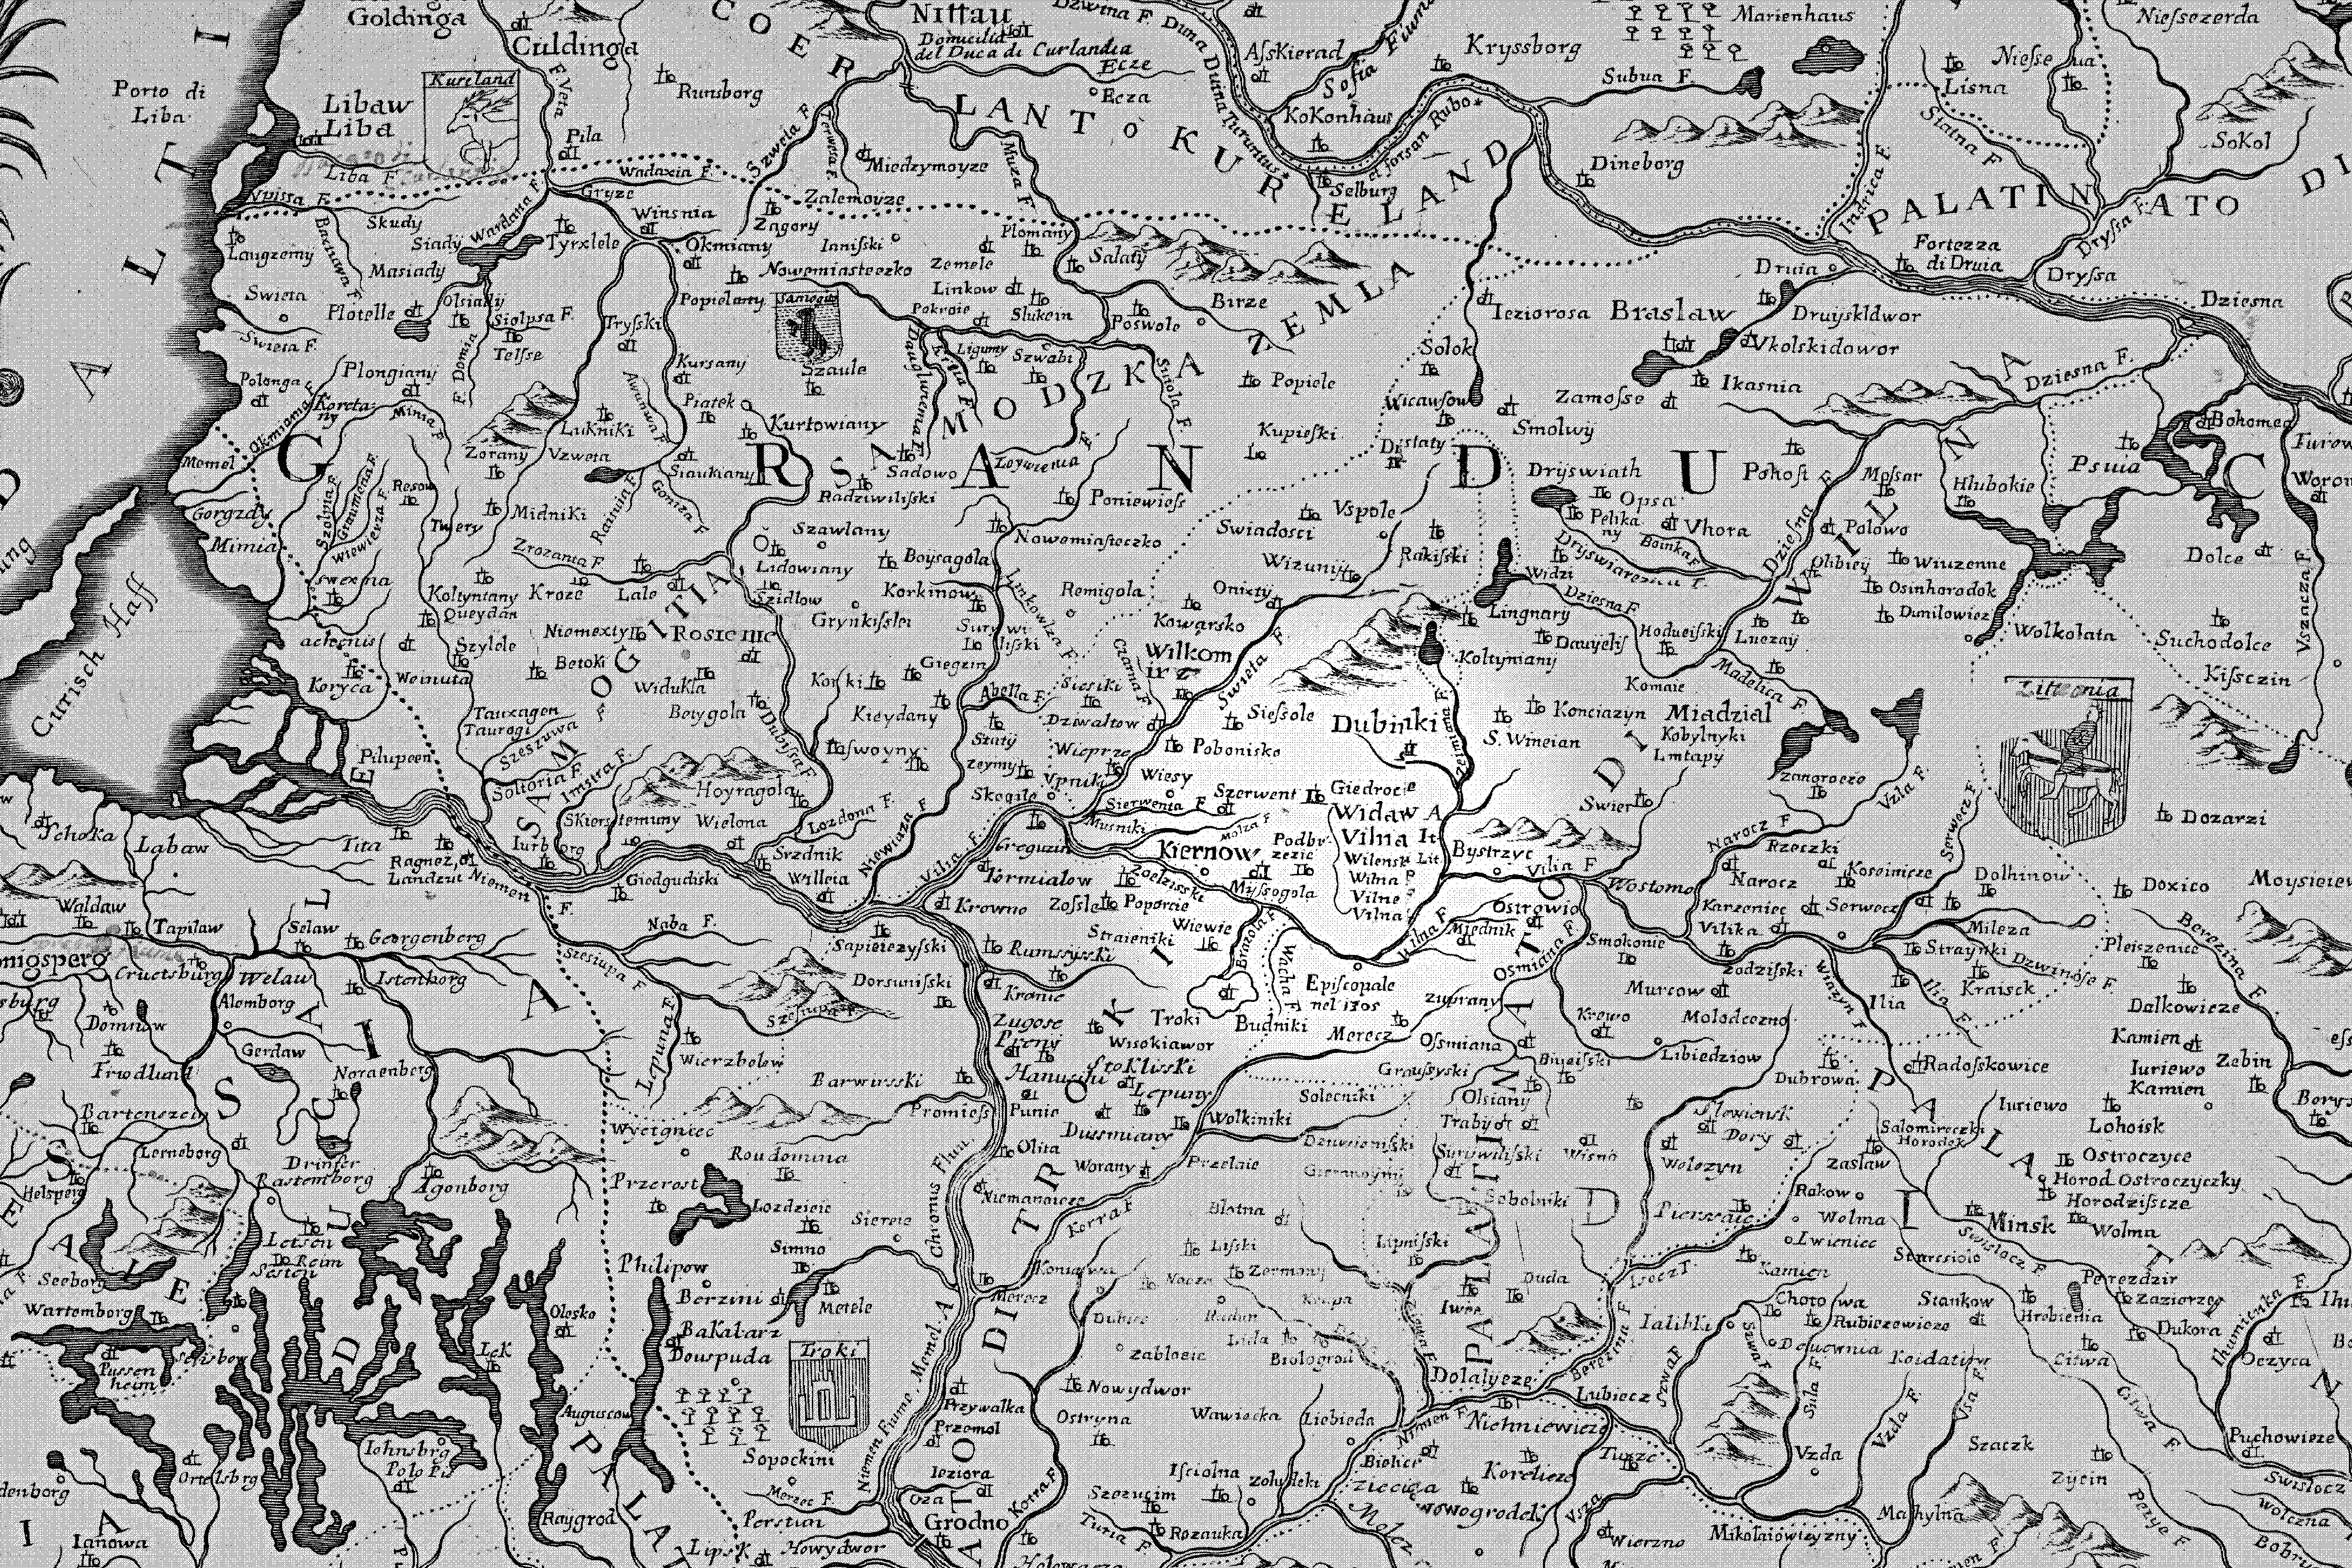
\includegraphics[width=10cm]{./ilustra-03.png} \footnotesize Detalhe de um mapa da Lituânia publicado em Veneza, Itália, em 1696.}
% \end{center}

\begin{figure}[!h]
    \centering
    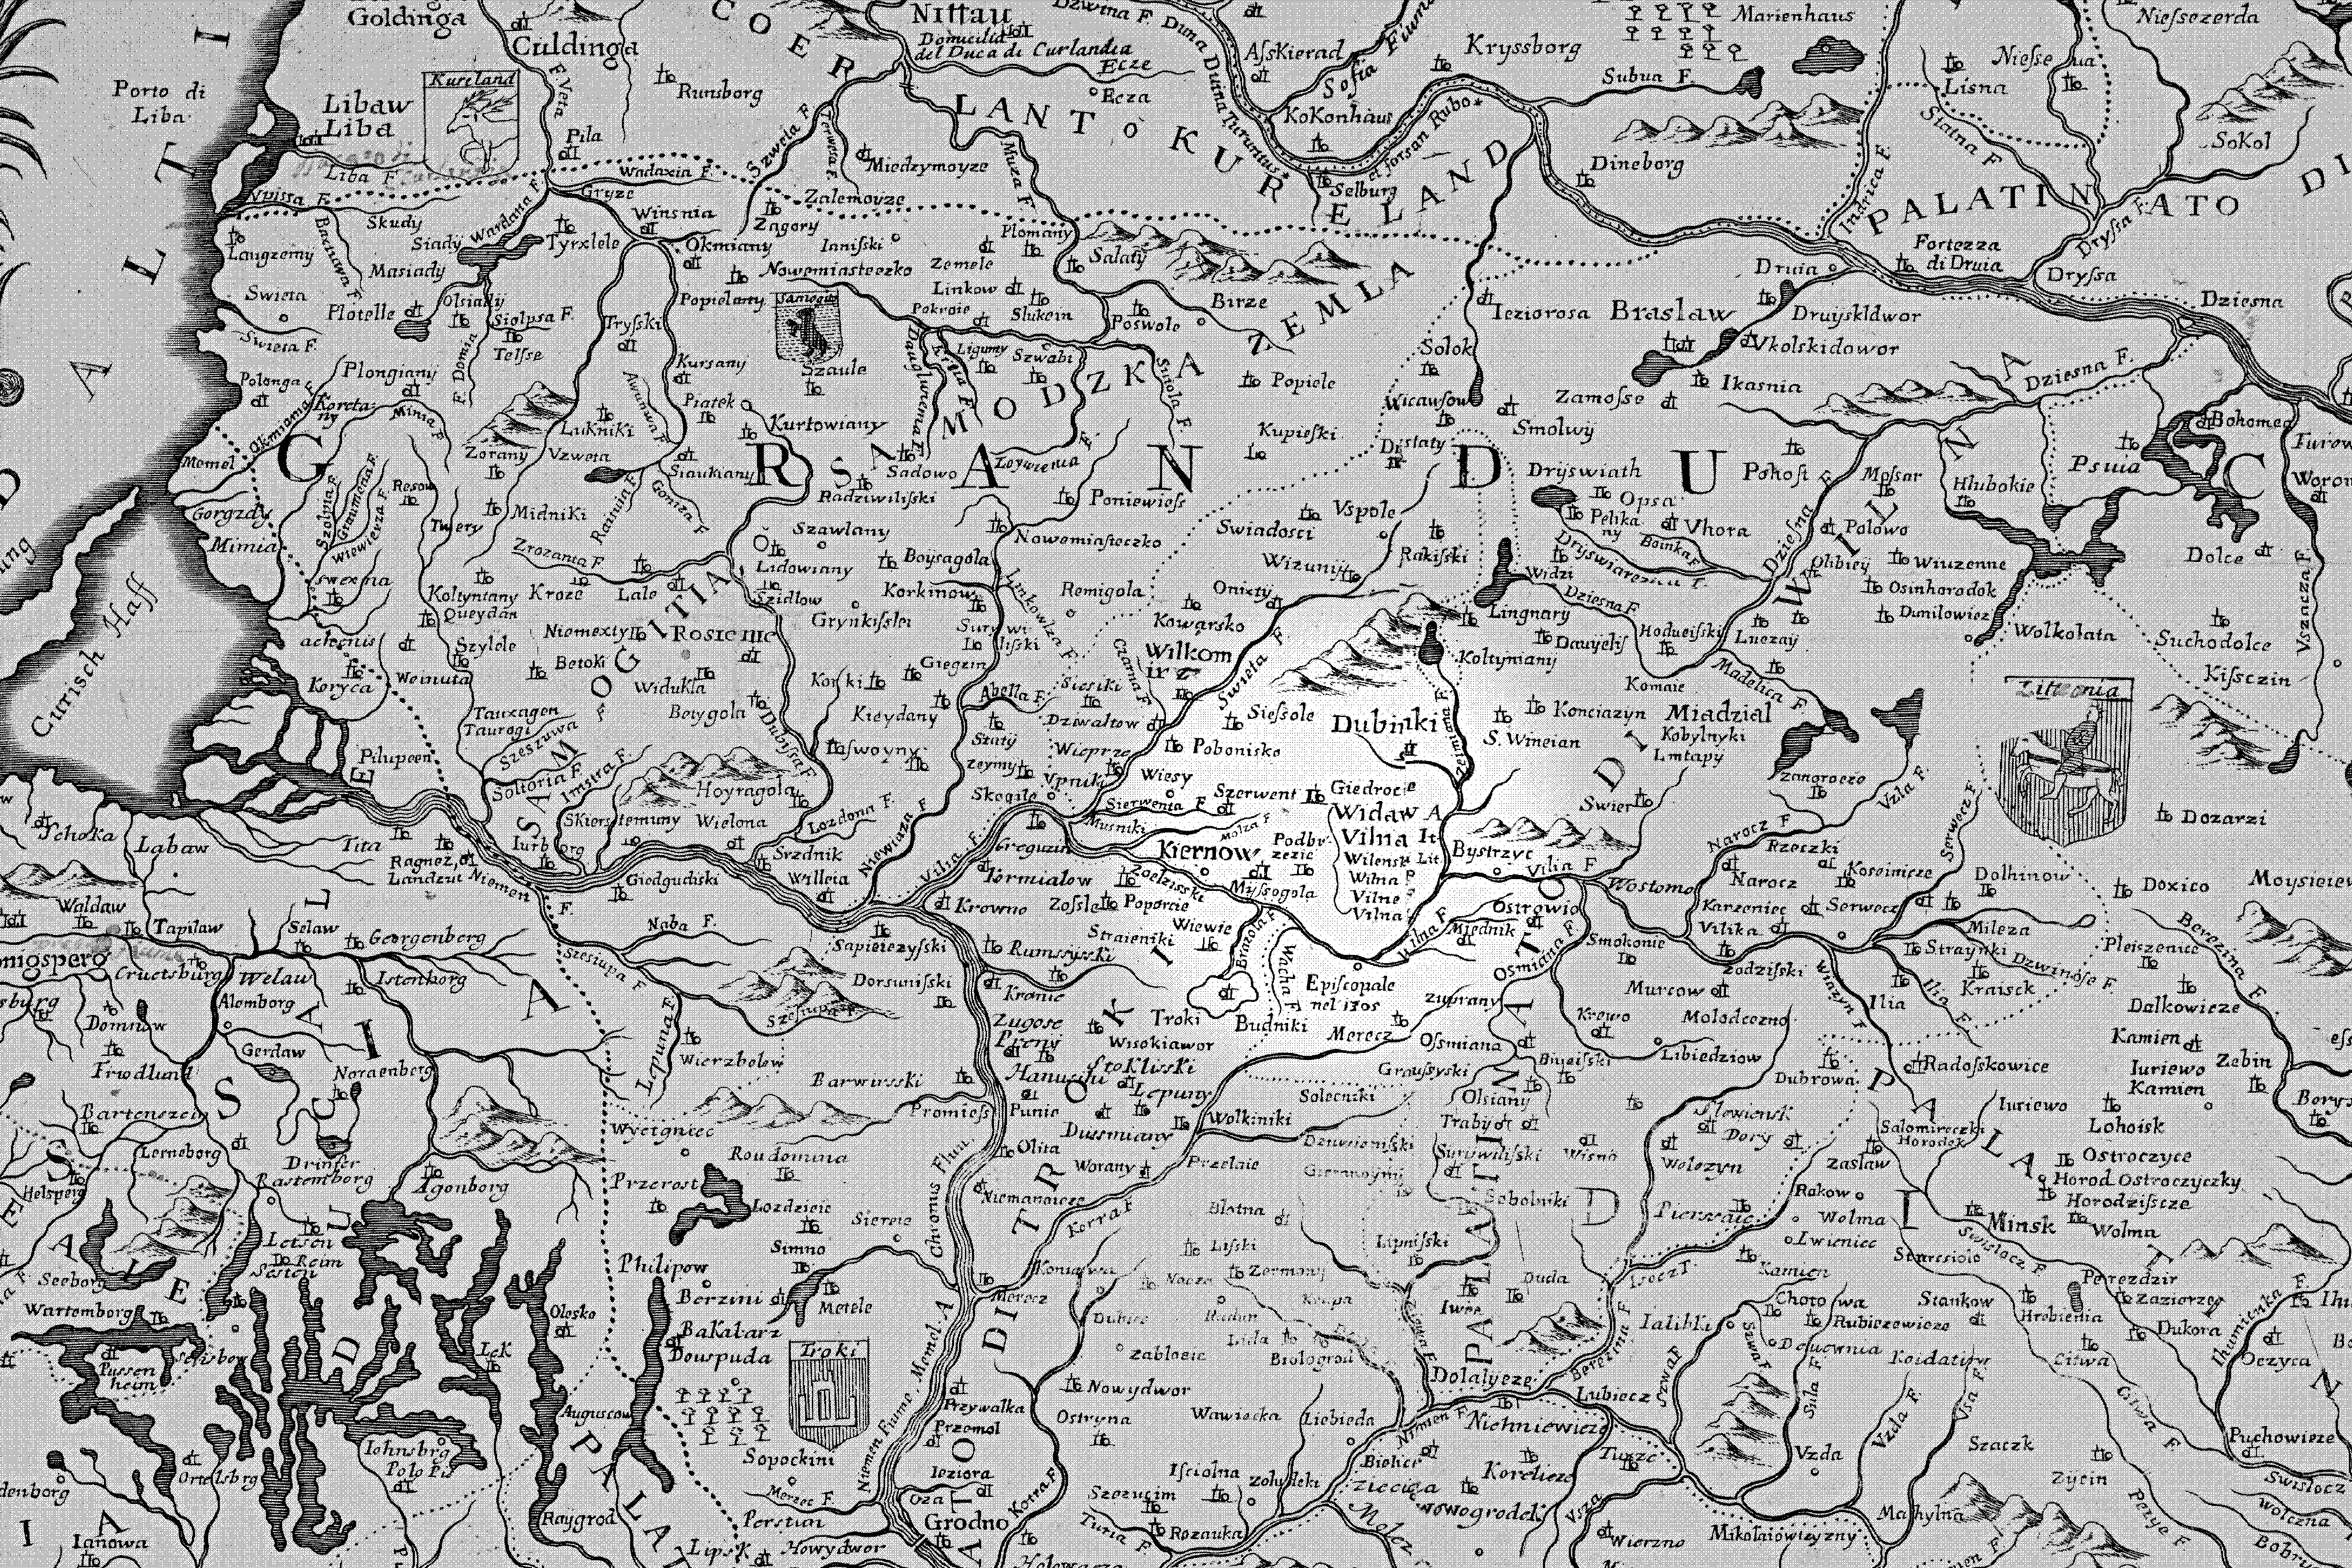
\includegraphics[width=\textwidth]{ilustra-03.png}
    \caption{Detalhe de um mapa da Lituânia publicado em 1696 em Veneza, Itália.}
\end{figure}

A Europa, na verdade, não é um continente, mas parte de uma entidade
geográfica muito mais vasta chamada Eurásia. O nome Europa tem origem
entre os gregos antigos, que a imbuíram do voluptuoso corpo da jovem
filha do rei de Tiro. A princesa Europa logo se tornou vítima dos ardis
dos deuses do Olimpo: acabou sendo seduzida e raptada por Zeus, que, com
o propósito de conquistá"-la, se metamorfoseou num deslumbrante touro
branco. Zeus cruzou o mar com uma Europa assustada montada sobre o seu
robusto dorso bovino, levando"-a, de sua terra natal na costa da Ásia
Menor, até Creta, onde, após um lúbrico instante de amor, ele a
transformou na rainha da ilha. Nascia, assim, com base numa lenda de
transgressão divina, a separação geográfica entre Ásia e Europa.
Enquanto o mito confere identidade à Europa, a história (ou, antes, uma
trama e uma leitura bem particulares dela) lhe concede características
geográficas específicas. Devido à falta de quaisquer fronteiras físicas
detectáveis, a delineação da Europa como continente separado surgiu
primeiramente como ideia de distinção geográfica. O mapa da Europa,
portanto, fala mais da ação da imaginação histórica do que de qualquer
outra força da natureza. Por conseguinte, a procura pelo centro da
Europa é, sobretudo, e, em primeiro lugar, uma jornada pela mentalidade
europeia.

A busca pelo centro começa sempre na demarcação das periferias, pois
nenhum ponto mediano pode ser encontrado antes que primeiro se
identifiquem e depois se meçam as margens. As beiradas seguram o centro,
dando"-lhe um sentido de gravidade, mantendo"-o vivo. Um centro sem
beiradas entra em colapso e se transforma num espaço contestado. Em
outras palavras, ele se transforma em fronteira. Encontrar o centro
cartográfico da Europa se depara com outro desafio, pois exige aferir os
parâmetros espaciais exatos de uma ideia. Destilar uma visão geográfica
numa série de números e conferir a ela uma expressão matemática faz com
que o projeto se torne uma interpretação cabalística do universo. Não
há, contudo, nenhuma fórmula secreta a se descobrir por trás de um
mapeamento científico da Europa. Suas extremidades periféricas são
determinadas pelos próprios geógrafos, que se valem da história e da
geopolítica como estrelas"-guias. O cálculo francês da Europa, que inclui
a Madeira e o arquipélago das Canárias --- tecnicamente parte da África
porém associados, do ponto de vista histórico e político, a estados
europeus --- não difere dessa lógica. Assim, indiretamente, a história,
passando pela geografia, localizou, perto de Vilna, o coração da Europa.
Esse posicionamento, entretanto, deve nos fazer lembrar de que a
história e a geografia jamais são escritas pelo mesmo povo. Por séculos,
Vilna viveu sob a sombra da Europa, e mesmo sua recém"-descoberta
importância continental só reafirma sua localização periférica dentro do
continente. A fronteira da União Europeia, recentemente traçada e
ratificada, dista cerca de trinta quilômetros a leste da capital
lituana, situando o centro do continente bem perto da Bielorússia, em
cuja fronteira se interrompe o atual projeto político de uma ``Europa
sem fronteiras''.

A relação centro"-periferia, contudo, jamais se refere tão somente ao
poder do centro e a submissão da periferia. As margens sangram na
direção do centro, subminando, assim, sem cessar, a sua influência, por
colocar em jogo suas próprias incertezas e inseguranças. O mesmo ocorre
com a centralidade marginalizada de Vilna: a cidade reúne a história da
Europa e a transmite por canais não"-cartografados. Nesse sentido, Vilna
representa mais um limiar do que um centro ou periferia. O limiar,
parafraseando Walter Benjamin, não é uma margem nem um ponto, mas uma
zona em que tempo e espaço se dilatam. Não é um lugar, mas uma condição,
``um fluido rompendo ou dividindo tendências extremistas'' que ``não
podem ser medidas nem localizadas.''\footnote{Renate Lachmann, \textit{Memory and Literature: Intertextuality in Russian Modernism}, trad. Roy Sellars e Anthony Wall. Minneapolis: University of Minnesota Press, 1997, p. 164.} Sentimentos sobre \textit{Wilno} (o nome polonês de Vilna) como local de limiar já foram expressos por Jan Bułhak,
célebre fotógrafo polonês do século \textsc{xx}, que falou de sua natureza
sinuosa, tentando capturá"-la em retratos hipnotizantes em preto e
branco. Bułhak colocou a cidade na paisagem fluida de uma alma humana,
fazendo dela um desafio aos parâmetros europeus, familiares e
inflexíveis, de tempo e espaço. \textit{Wilno}, nas palavras do fotógrafo, é uma
\textit{suspension of disbelief}:

\begin{quote}
A verdadeira \textit{Wilno} permanece calada e inacessível aos esnobes. Será que
vale a pena revelar seus verdadeiros tesouros para vândalos caçadores de
lembrancinhas e bestas ignorantes? A cidade fala com delicadeza sobre
coisas simples e nobres, e não se abre para qualquer um. Ela não grita
como um mascate nem faz alarde de seus próprios méritos --- ela
simplesmente conduz o viajante de mente aberta rumo a uma revelação.
Diversas pessoas vindas de terras longínquas conseguiram encontrar a
\textit{Wilno} autêntica e, para várias delas, o encontro com a cidade constituiu
uma grande experiência espiritual. Esses visitantes permanecem leais à
cidade até o fim da vida, louvando"-a de modo inteligente nas linguagens
da arte. Claro, houve também inúmeros visitantes indiferentes, que foram
embora com um sorriso zombeteiro. Eles só foram capazes de ver, porém, a
sua simplicidade, as suas deficiências e as suas imperfeições, e jamais
saberão que um encontro com \textit{Wilno} é na verdade um julgamento da alma, um
teste de percepção humana. Um tal teste é sedutor para alguns, mas, para
outros, os não"-iluminados, não passa de uma armadilha arriscada.

Eis então a nossa \textit{Wilno}: há quem diga que a cidade seja suja, pobre e
entediante; outros garantem que seja um lugar adorável, excepcional e
sublime. O que poderíamos dizer sobre ela hoje? De que lado devemos
começar a investigação da nossa \textit{Wilno}, profundamente mergulhada num vale
formado por dois rios, rodeada por colinas verdejantes e adornada por
graciosas torres de igreja no formato espiralado de álamos de uma antiga
casa senhorial?

Não nos apressemos para dentro da cidade, demoremo"-nos por um momento no
seu limiar. Wilno se espalha entre as colinas, permitindo ser observada
prazerosamente de longe. Gozemos portanto desse prazer de contemplar a
cidade à distância.\footnote{Jan Bułhak, \textit{Vilniaus peizažas: fotografo kelionės}. Vilna: Vaga, 2006, pp. 21--23.}
\end{quote}

\asterisc

Este livro fala de distância, suspensão e descoberta, fala do momento do
limiar --- uma zona não"-cartografada --- que separa Vilna de seus visitantes
estrangeiros. É uma narrativa da cidade do ponto de vista de um
estrangeiro, com sua história detalhada pela geografia de reflexões
íntimas, relatos oficiais, cartas particulares, relatórios
jornalísticos, observações militares e narrativas de viagem de seus
inúmeros visitantes. Este livro, portanto, não é só sobre Vilna, mas
também sobre a Europa. É um mapa de todo o continente, percorrido pelas
ruas de Vilna.

Vilna sempre ofereceu uma ligação crítica entre diversos componentes,
nações e interpretações da Europa. A cidade foi freqüentemente retratada
como ponte entre Oriente e Ocidente, mas, assim como todo lugar
estrategicamente ambíguo, ela também tem sido um local altamente
contestado. Por conseguinte, a cidade jamais possuiu uma única
identidade. 

O lugar fala da \textit{Vilne} judaica, da \textit{Wilno}
polonesa, da \textit{Vilna} russa e francesa, da \textit{Wilna} alemã, da
\textit{Vilno} bielorrussa e da \textit{Vilnius} lituana. Esses diversos
reinos topológicos comungam talvez do mesmo território, mas conduzem na
direção de experiências e memórias surpreendentemente distintas. No
início, o objetivo deste livro era confrontar, comparar e, se possível,
sincronizar as diferentes articulações da cidade. Como geógrafo
histórico e cultural, quis mapear a paisagem urbana encontrando fios
narrativos específicos que entrelaçam suas várias fronteiras
linguísticas, religiosas e ideológicas. Nesse intuito, li e percorri
toda uma gama de narrativas oficiais e pessoais. E, a cada nova excursão
linguística ou ideológica, eu era conduzido na direção de uma trajetória
geográfica diferente do lugar. Meu canteiro de pesquisa --- a cidade de
Vilna --- se dispersava diante dos meus próprios olhos e, ao invés de
chegar ao ponto em que se intersectam as representações da cidade,
via"-me sempre deixando a cidade através de um de seus diversos portões
narrativos.

Num determinado momento, em meio à minha investigação, fui capaz de
compreender que o que eu vinha identificando não eram interpretações
disparatadas de Vilna, mas representações centrífugas da Europa. A razão
de não poder encontrar o tema histórico central, comum a todas aquelas
narrativas urbanas, era muito simples: eu buscava a unidade da cidade em
mapas diferentes da Europa. Assim, ao invés de sair de Vilna mapeando
trajetórias separadas de narrativas locais dispersas, decidi entrar na
cidade a partir dos diferentes pontos culturais e ângulos linguísticos
da Europa. Como consequência, o epicentro da minha investigação se
deslocou da busca por um nexo narrativo de Vilna para questões
relacionadas à ideia sempre mutável de Europa.

Embora a alteração analítica modificasse o curso de minha pesquisa, ela
não mudava a intenção de minhas explorações. Vilna, com sua paisagem
cultural formada por inúmeras camadas, permanecia o ponto focal de meus
interesses, mas orientei minha pesquisa na direção do diálogo entre a
geografia da Europa e a história de Vilna, fazendo disso uma estória de
interação entre significados locais e suas interpretações estrangeiras.
Não obstante, a reversão do fluxo investigativo inevitavelmente
transformou o terreno expositivo da cidade: de um lugar nativo, familiar
e mundano, Vilna se converteu num local estrangeiro, estranho e até
mesmo exótico. Apesar disso, acredito que algumas características da
minha compreensão nativa da cidade sobreviveram a tal transposição,
simplesmente devido ao fato de o meu objetivo analítico inicial e o meu
conhecimento pessoal do lugar terem me posicionado, por assim dizer, no
lado aborígene do espelho representacional. Essa busca nativa pela
Europa em Vilna atirou uma nova luz sobre as implicações locais de
várias batalhas políticas, fricções ideológicas e colisões culturais de
proporções continentais. Ela também me conduziu até novas fronteiras
teóricas e narrativas da investigação geográfica, pois me permitiu
traçar e refazer as experiências dos viajantes de uma maneira mais
dinâmica e imaginativa. O livro se baseia em relatos escritos sobre
Vilna, que de maneira alguma desembocam num mapa definitivo do lugar. O
que ele gera, porém, não é menos real, na medida em que aviva a história
local com as vozes, experiências e fantasias dos viajantes que
utilizaram a cidade como pouso em suas andanças de auto"-conhecimento. Em
suma, minha narrativa de Vilna é uma estória de viagem, uma história da
cidade cartografada como passagem de um mundo familiar para um reino
desconhecido.

Vilna jamais foi uma cidade cobiçada pelos viajantes e, à diferença de
outras cidades mais celebradas da Europa, tais como Roma, Paris,
Londres, Berlim, Viena ou Moscou, ela jamais reuniu um cânone narrativo
e representacional que pudesse guiar os visitantes estrangeiros através
de sua história e geografia. A história de Vilna espelha a da Europa,
mas apenas como um eco alterado e distorcido de sua estória grandiosa.
Claro está que cada canto da Europa tem sua voz própria, capaz de
determinar o ritmo unificador ligeiramente desafinado do continente.
Nessa polifonia, porém, de variações reverberantes, Vilna interpreta uma
toada perfeitamente excêntrica. Embora a história da cidade esteja
repleta de mudanças dramáticas e com frequência trágicas, acontecimentos
e personalidades locais raramente participam do vocabulário histórico
comungado por toda a Europa. E, até hoje, Vilna se apresenta como um
forasteiro continental, um personagem pouco familiar --- um transgressor ---
no seio de um esmerado \textit{storyboard} da Europa.

Essa ausência de uma familiaridade europeia não significa que os
encontros de Vilna com forasteiros tenham sido poucos. Pelo contrário,
durante sua história secular, a cidade sofreu inúmeras invasões
estrangeiras, a maior parte delas em períodos de guerra e ocupações.
Devido ao caráter fronteiriço desses encontros, Vilna foi raramente
vista ou vivenciada como um destino em si mesmo --- e sim como um lugar de
passagem, um espaço que conduz a outros fins, em outras palavras, um
limiar. A natureza transitória e inadvertida dos visitantes de Vilna
deram contorno àquilo que os estrangeiros passaram a conhecer sobre o
local. Os estrangeiros, em Vilna, são mais como coletores (ou, pior,
forrageadores), que veem, imaginam, e frequentemente vivenciam o lugar
como se fosse a sobra de uma colheita histórica --- europeia --- muito mais
grandiosa. Embora tenha me utilizado de estrangeiros como narradores da
cidade, este livro constitui menos uma tentativa de modificar essa
noção, do que expor o outro lado dela. Enquanto as opiniões dos
estrangeiros tendem a marginalizar Vilna, suas narrativas, quase sempre
involuntariamente, acabam posicionando a ideia e a prática europeias no
centro da história local. Em outras palavras, tornei central tudo aquilo
que os estrangeiros viram como periférico.

A inversão da hierarquia representacional me permitiu facilitar a
separação entre estrangeiros e nativos, a qual, de certa maneira,
corresponde à transformação histórica de Vilna. História e geografia
transformaram a cidade num lugar de migrantes, em que as experiências de
estrangeiros e habitantes locais, recém"-chegados e residentes,
expatriados e nativos se fundem numa miríade de narrativas e memórias
entrelaçadas que podem facilmente transgredir diferentes ordens
temporais e espaciais. De certo modo, qualquer um pode ser um
estrangeiro em Vilna, não devido a sua origem estrangeira, mas porque a
cidade possui tantos nomes e tantas histórias que uma única identidade
humana mal pode abarcá"-los todos.

Diferentes vozes estrangeiras e línguas nativas tornam difícil localizar
Vilna num único mundo ortográfico. Ao longo do texto, tentei usar o nome
de Vilna conforme encontrado nas fontes originais; assim, o nome da
cidade alterna entre sua versão lituana contemporânea e versões mais
precisas do ponto de vista histórico, linguístico e pessoal, como por
exemplo \textit{Wilna}, \textit{Vilna}, \textit{Vilne} e \textit{Wilno}. O mesmo
é válido para todos os outros nomes locais de lugares e pessoas. Com
vistas a auxiliar o leitor a navegar com maior suavidade por esse
arquipélago de diferentes marcas ortográficas, um índice contendo todas
as versões dos topônimos está à disposição no fim do livro.

\chapter{A margem da Europa}

%\setlength{\epigraphwidth}{.45\textwidth}
\begin{epigraphs} 
\qitem{Talvez virmos de uma região que por um longo período foi considerada os
confins orientais de uma Cristandade centrada em Roma nos torna mais
sensíveis aos pontos de gravidade mutáveis, simbolizados pela própria
fluidez de termos tais como Ocidente e Oriente.}{\textsc{czesław miłosz}}
\end{epigraphs}

O aparecimento de Vilna na Europa constituiu uma anomalia espiritual ---
cidade pagã num oceano de cristandade. Uma epístola, recebida em 1323
pelo papa na cidade meridional de Avignon, anunciou o nascimento de
Vilna. Levada por um monge austero do porto báltico de Riga, a carta
chegou ao palácio papal de pedra cinzenta com os primeiros sopros
arrepiantes do mistral. A chegada do mistral geralmente coincidia com o
Advento e o início de um novo ciclo no calendário católico. A
correspondência, supostamente redigida por Gediminas, o auto"-intitulado
``rei dos lituanos e de muitos russos'', prometia também um novo começo.
Num texto elaborado num latim diplomático, o rei lituano solicitava ao
papa --- ``o mais excelso padre do trono romano'' --- que aceitasse sua
submissão real e recebesse a si e seus conacionais na comunhão cristã
dos santos. O pedido rejubilou o Papa João \versal{xxii}, que anos a fio havia
fracassadamente tentado convencer Gediminas a receber o batismo
católico. A carta, porém, não estava assinada, não estava datada, nem
continha marcas nítidas de sua origem geográfica ou de seu remetente.
Essa falta de cortesia epistolar fez com que ela parecesse pouco
convincente, se não mesmo falsa, de modo que o papa leu a mensagem com a
prudência de uma incerteza política.\footnote{Carta de Gediminas ao Papa João \versal{xxii} em \textsc{v}.\,Pašuta e \textsc{i}.\,Štal, \textit{Gedimino laiškai}. Vilna: Mintis, 1966, p. 22.}
Havia motivos de sobra para desconfiar de Gediminas. Um deles era o fato
de ele ser pagão --- o último governante pagão ainda existente na Europa.
Pior ainda, a sua propriedade --- a Lituânia --- era um estado apóstata. No
meio do século \textsc{xiii}, seu governante, Mindaugas, recebera o batismo do Papa
Alexandre \versal{iv}, para dois anos mais tarde renunciar à fé. Por mais de um
século, os lituanos haviam sido inimigos mortais dos católicos, atacando
seus castelos, pilhando suas cidades recém"-construídas, incendiando suas
igrejas, massacrando padres e escravizando neófitos nas fronteiras
bálticas da cristandade. Os papas repetidamente convocavam guerras
santas contra eles. A Ordem Teutônica, desalojada da Terra Santa em
consequência da perda de Jerusalém, liderou a Cruzada Nórdica.

A Ordem era uma instituição monástica, cujos membros faziam voto de
castidade como penitência por seus pecados. Os cavaleiros teutônicos,
assim como vieram a ser conhecidos, formaram uma irmandade de guerreiros
penitentes que levavam na mão a cruz com uma espada, garantindo assim a
redenção pessoal com o sangue dos infiéis, hereges e apóstatas. Depois
de viajar do Mediterrâneo até as costas do Báltico na virada do século
\textsc{xiii}, a Ordem Teutônica havia se transformado numa eficiente máquina
militar com a missão apostólica de disseminar e defender a fé católica
entre os gentios. Uma sucessão de papas os benzeram com absolvição,
garantindo sua devoção à Igreja Mãe, e diversos imperadores do Sacro
Império Romano Germânico lhes concederam vastos territórios, tornando a
Ordem um dos maiores domínios feudais da Europa. Como sinal de sua
privilegiada posição social e religiosa, a aristocracia europeia
multilíngue acumulou"-os de doações financeiras e de um crescente excesso
de filhos ociosos. Apesar do apoio cosmopolita, a Ordem Teutônica deveu
sua força numérica à populosa classe aristocrática da área germanófona;
daí o seu nome. Como resultado, seu zelo missionário foi matizado pelas
cores do expansionismo feudal, da repressão social e da transformação
cultural. Junto com a cruz, os cavaleiros levavam progresso alemão à
região báltica, construindo sólidos castelos, cidades comerciais,
mansões nobiliárquicas e paróquias católicas em troca de sua dominação.
Os monges"-guerreiros eram seguidos por colonos alemães leigos das
cidades hanseáticas, fazendo da missão religiosa um movimento
colonizador, que foi batizado, na época nacionalista e romântica do
século \textsc{xix}, como \textit{Drang nach Osten}, o impulso para o leste.

Os cavaleiros, investidos com o poder do apoio tripartite da igreja, do
imperador e da aristocracia, construíram um estado fortificado na
Livônia e na Prússia, territórios conquistados localizados nas
fronteiras setentrionais e ocidentais da Lituânia, isolando assim,
efetivamente, o país pagão da Europa latina. No decorrer de uma ou duas
gerações de acúmulo de riqueza e prestígio, a Ordem se tornou cada vez
mais independente de seus benfeitores. Os monges governavam as terras
bálticas conquistadas sem qualquer lealdade às autoridades imperiais ou
eclesiásticas. Encorajados pelo êxito político, heroísmo militar e
astúcia comercial, eles demonstraram pouco respeito às complexas
hierarquias da Europa latina. As maneiras arrogantes da Ordem não
passaram despercebidas. Enquanto o Papa João \versal{xxii} chamava os cavaleiros
com frequência de amados filhos da igreja católica, eles recebiam pouca
afeição do rei da França, tesoureiro do papado.

O Papa João \versal{xxii}, francês de origem modesta, foi eleito em 1316 para
servir aos interesses da coroa francesa, que havia levado o papa
anterior de Roma para Avignon, cidade localizada no sul da França.
Apesar da idade --- João \versal{xxii} contava quase setenta anos à época de sua
eleição --- o papa não demonstrava sinais de letargia. Na Itália, liderou
uma longa e brutal cruzada contra os estados locais que se opunham a um
papado dominado por franceses. Durante a guerra, ele excomungou Ludwig
da Bavária, incansável adversário do trono do Sacro Império Romano
Germânico e principal instigador da liga anti"-papal na Europa. O Papa
João \versal{xxii} se dedicou também a limpar a igreja de inúmeros desvios
dogmáticos. O édito que definiu o seu papado foi a excomunhão de um ramo
influente de irmãos franciscanos, conhecidos como espiritualistas,
devido à sua adesão a princípios de pobreza evangélica baseada na
convicção de que Jesus e os Apóstolos não detinham posses materiais. Num
gesto oposto, em julho de 1323, ele transformou Tomás de Aquino, o
\textit{Doctor Angelicus} do conhecimento teológico, em santo.

Logo após ler a primeira carta de Gediminas, o pontífice recebeu a
visita de uma delegação vinda de Riga, trazendo mais uma epístola do
governante lituano. Gediminas culpava a política agressiva dos
cavaleiros teutônicos pela teimosa rejeição da fé católica por parte dos
lituanos. Todavia, o papa não precisava duvidar da intenção de Gediminas
de receber o batismo. O Papa João \versal{xxii} foi ainda informado pelos
delegados que Gediminas havia alardeado sua futura conversão a todo o
resto da Europa. O rei havia despachado diversas outras cartas,
dirigidas a ``todos os cristãos, homens e mulheres, espalhados pelo
mundo'', em que anunciava a aguardada chegada dos representantes papais
à Lituânia. De maneira estratégica, os principais destinos dessa
importante difusão se restringiam às ``prestigiosas cidades de Lübeck,
Stralsund, Bremen, Magdeburgo e outras louváveis cidades entre Colônia e
Roma.'' Gediminas informou também as maiores casas monásticas católicas
--- as Ordens Franciscana e Dominicana --- de seu desejo de se tornar
cristão, convidando membros da irmandade a viajar até seu reino e
disseminar a palavra e as boas ações entre seus súditos. Conforme a
prática vigente aplicada a importantes notícias públicas, Gediminas
pediu aos destinatários anônimos de suas mensagens que duplicassem a
carta e que, depois que uma cópia fosse pregada na porta principal da
igreja mais próxima, a transmitissem pela rede postal da Europa medieval
para a próxima cidade ou mosteiro. Dessa maneira, declarou o autor da
mensagem, ``a glória de Deus'' poderia ser compartilhada por todos. As
intenções sagradas de Gediminas foram acentuadas pela data
cuidadosamente escolhida para o seu comunicado. O primeiro pacote de
cartas foi assinado em 25 de janeiro, dia que celebra a conversão do
Apóstolo Paulo, responsável pela disseminação da fé cristã entre os
gentios. A segunda remessa foi timbrada em 26 de maio, dia de
Corpus Christi, homenageando o sacramento da Eucaristia e o
milagre da transubstanciação do corpo de Cristo.\footnote{Carta de Gediminas à burguesia de Lübeck, ibid., pp. 28--35.}
Antes que as cartas chegassem à sua pretendida audiência cristã, a
cidade de Vilna era um lugar anônimo e desconhecido. Um assentamento
humano deve ter existido no local muito tempo antes de Gediminas chegar
ao poder em torno de 1315, mas foram suas palavras conciliatórias
dirigidas à Europa latina que propiciaram a existência do lugar no
registro histórico da Europa. Por conseguinte, a idade de Vilna é
contada a partir de 1323, fazendo"-a tão velha quanto a santificação de
Tomás de Aquino.

\asterisc

O nascimento de Vilna de que se tem registro se apoia num mito local. Em
geral, as lendas são muito mais antigas que documentos; no caso de
Vilna, porém, a distância temporal entre o mito e o arquivo é
insignificante. Na verdade, é possível que o mito da origem da cidade
tenha sido inventado em resposta à sua fundação documental. Isso poderia
explicar o fato de que a lenda e o registro tenham o mesmo protagonista:
Gediminas, confrontando o mesmo dilema geopolítico de como fazer a
Lituânia uma nação aceita e reconhecida no mundo. Tanto o mito como os
registros históricos --- as cartas --- procuram estabelecer uma ligação
entre o universo local e o universo estrangeiro por meio da construção
de Vilna como terreno em que duas esferas se encontram.

Vilna, reza a lenda, nasceu de um sonho. Enquanto caçava nos densos
bosques que viriam a circundar a futura cidade, Gediminas, exausto,
resolveu descansar. Durante o sono, ele teve a visão de um lobo de ferro
uivando com ferocidade. Estupefato diante de imagem tão incomum,
Gediminas pediu uma explicação ao sacerdote pagão. O oráculo interpretou
o sonho do rei como um desafio ao seu dever cívico. O sacerdote instruiu
o rei no sentido de erguer uma cidade no mesmo lugar em que tivera o
sonho, cidade que traria fama mundial para o seu nome e para a Lituânia.
Gediminas não perdeu tempo e de imediato metamorfoseou a sua visão em
pedra. Um castelo imponente foi construído na colina mais alta diante da
confluência de dois rios, em torno de cujos leitos tortuosos a cidade se
estabeleceu.

\textit{Vilnius} muito provavelmente tomou emprestado seu nome ao menor dos dois
rios, o \textit{Vilnia}, que conota um fluxo ondulado, meândrico e sinuoso
em lituano. O nome também aponta para a proximidade com o outro mundo.
Os vocábulos lituanos para defunto ou \textit{velionis}, fantasma ou \textit{vėlė}; 
e diabo ou \textit{velnias}, comungam da mesma raiz
etimológica de \textit{Vilnius}, que abrigou um dos mais sagrados locais da
Lituânia pagã. A palavra \textit{Vilnius} indica características excepcionais ou
mesmo mágicas do lugar. Denota uma ligação entre reinos do universo
distintos e opostos, que faz de Vilna um local pulsante --- mais como um
instante no tempo do que um lugar físico --- que serve de ponte entre os
vivos e os mortos.\footnote{Para maiores informações sobre os significados mitológicos de Vilna, ver Vladimir Toporov, ``Vilnius, Wilno, Vil'na: miestas ir mitas'' em \textit{Baltų mitologijos ir ritualo tyrimai}. Vilna: Aidai, 2000, pp. 35--98.}
A etimologia (nome), a lenda (narração) e a história (registro factual)
de Vilna revelam suas origens nativas. Diversas cidades erguidas nas
fronteiras bálticas da cristandade, tais como Riga, Tallinn e
Königsberg, foram fundadas no intuito de expandir e fortalecer a
hegemonia estrangeira sobre as terras conquistadas e os povos
aborígenes. Em corpo e espírito --- ou seja, na redação jurídica e no
funcionamento social --- elas eram cidades coloniais. Vilna foi diferente
--- autóctone, pagã e livre, ela foi capaz de fortalecer tradições locais.
O lugar se tornou capital da Lituânia em resposta às intrusões
estrangeiras. Portanto, se a espiritualidade pagã foi a madrinha de
Vilna, então o longo e estafante conflito militar contra o mundo
católico foi o seu padrinho. Gediminas elegeu Vilna como residência real
por estar profundamente localizada no interior da Lituânia, protegida
não só por deuses pagãos, por um exército eficiente e por um sistema de
vigilância bem situado, como também por vastas florestas, rios
tortuosos, terrenos pantanosos instáveis e um tempo caprichoso --- tudo
tornando o acesso estrangeiro à cidade numa tarefa extenuante.

%{[}figura 5{]}
%
%Gediminas constrói um castelo no mesmo lugar em que teve o sonho:
%representação romântica, do século 19, do mito fundador de Vilna.

Malgrado o isolamento geográfico e as qualidades defensivas do lugar,
Gediminas imaginou Vilna como um terreno europeu de convergência. Nas
cartas em que prometia sua conversão, ele convidou os católicos da
Europa --- comerciantes, cavaleiros, clérigos e artesãos --- a se
estabelecer na recém"-consagrada capital da Lituânia. Prometeu aos
recém"-chegados privilégios exclusivos de natureza religiosa, legal e
cultural, junto com um solene pedido de lealdade e respeito às tradições
pagãs locais. Assim, o único grupo explicitamente excluído de sua
generosa oferta foram os monges guerreiros da Ordem Teutônica.

No militante zelo de sua atividade missionária, os cavaleiros, claro,
eram os mais vociferantes opositores da conversão pacífica e diplomática
da Lituânia. Tendo escolhido o caminho da redenção por meio de um
evangelismo bélico, eles estavam determinados a manter o paganismo na
Lituânia. Os cavaleiros viam no estabelecimento, sem a sua participação,
de uma comunidade cristã em Vilna um desafio frontal à sua sobrevivência
política e pessoal. Sem a presença ameaçadora dos gentios lituanos, a
Ordem corria o risco de acabar violentamente, assim como ocorrera com os
Templários, cuja irmandade fora brutalmente esmagada por Clemente \versal{v}, o
papa precedente, que acatara as calamitosas acusações do rei francês.
Felizmente para a irmandade teutônica, o novo rei da França, o jovem e
grosseiro Charles \versal{iv}, estava de novo planejando libertar Jerusalém do
jugo muçulmano, demonstrando, por conseguinte, pouco interesse pelas
questões bálticas. O francês deixou o assunto da conversão lituana nas
mãos do papa, que ainda guardava no seu íntimo um resto de afeto pelo
zelo missionário dos cavaleiros.

A fim de acentuar sua necessidade mundana, a Ordem Teutônica dedicou a
Lituânia livre à Virgem Maria. O gesto devocional fez da hegemonia
política sobre o país uma questão espiritual. O imperador do Sacro
Império Romano Germânico sancionou a barganha celestial, mas o papa
discordou, pois não se via disposto a repartir as honras da conquista
espiritual com as exigências políticas dos cavaleiros. O Papa João \versal{xxii}
tencionava manter a soberania da Lituânia por tanto tempo quanto seus
governantes aceitassem o catolicismo. Da distante Avignon, ele mandou
duas cartas: uma para Gediminas, louvando sua decisão de abraçar o
catolicismo, e outra para os cavaleiros teutônicos, repreendendo"-os pela
insubordinação. O papa enervou os cavaleiros por insistir num acordo de
paz de seis anos entre a Lituânia pagã e as potências católicas vizinhas
com vistas a atingir o objetivo da conversão. Relutante, a Ordem
Teutônica admitiu a derrota diplomática.

Na primeira metade do século \textsc{xiv}, o estado da cristandade se encontrava
longe do ideal. Diferenças doutrinárias irreconciliáveis entre católicos
e ortodoxos mantinham os cristãos numa divisão permanente. Entre os
católicos, divisões teológicas e animosidades feudais não eram menos
danosas. O papado não passava de uma mercadoria religiosa a ser
negociada, comprada, usurpada e obtida à força, ou simplesmente
desposada. O Vigário de Cristo era mantido debaixo dos olhos vigilantes
e da bolsa controladora da coroa francesa no exílio dourado de Avignon.
Em questões políticas, o papa deve ter"-se sentido uma nulidade. De
maneira providencial, a conversão da Lituânia propiciou uma oportunidade
única para a restauração da autoridade espiritual e da posição social do
papa. A Lituânia se localizava na convergência de diversas órbitas
religiosas, militares e comerciais da Europa, numa região em que
interesses de diferentes potências políticas e autoridades religiosas se
sobrepunham. Enquanto pagãos, os governantes lituanos expandiram
profundamente seu controle político pelas províncias eslavas cristãs. No
oeste e ao norte, esse estado próspero era limitado por países
católicos; no leste e ao sul, ele se misturava às províncias ortodoxas
da Rússia; e em suas extremidades a sudeste, ele atravessava os domínios
tributários dos canatos mongol"-tártaros. O batismo latino teria
inevitavelmente feito da Lituânia um baluarte do catolicismo numa região
de lealdades religiosas instáveis, e poderia ter criado o ambiente
perfeito para uma interessante união entre adeptos dos ritos grego e
latino sob os auspícios do papado. O papa não tinha como imaginar que
seu caminho rumo a uma posteridade de beatitude, e mesmo de santidade,
poderia passar pela imersão batismal do remoto rei pagão da Lituânia.

%{[}figura 6{]}
%
%Lituanos pagãos adorando o fogo, o carvalho e a serpente do Paraíso, em
%\textit{La cosmographie universelle}, 1556.

Para uma missão tão crucial, o Papa João \versal{xxii} selecionou três
representantes: dois proeminentes teólogos franceses --- um bispo e um
abade, ambos membros da Ordem Beneditina --- e o arcebispo de Riga,
presumido padrinho espiritual de Gediminas, que havia sido também
enviado para assumir sua distante sede após anos de exílio devido ao
contínuo conflito entre a Ordem Teutônica e a hierarquia da igreja
católica local. Após uma árdua viagem por terra e mar, os representantes
chegaram a Riga, capital da Livônia, no início do outono de 1324.
Encontraram uma cidade em tumulto. Uma guerra de baixa intensidade
estava fervendo entre os cavaleiros teutônicos, que haviam tomado o
controle político e eclesiástico da Livônia, e a burguesia de Riga, que
tentava proteger os privilégios civis e os interesses comerciais da
crescente classe mercantil. O arcebispo tomou o partido dos
comerciantes, que, por sua vez, procuraram apoio militar dos lituanos
pagãos. Antes que um tratado de paz fosse assinado em Vilna, uma aliança
blasfema entre pagãos e burgueses católicos emergiu contra os irmãos
teutônicos. Diante da nova crise gerada por tal ímpia união, os
representantes mandaram um emissário até Vilna a fim de preparar o
terreno para a conversão cerimonial de Gediminas.

Na região báltica, a melhor época para se viajar por terra era no meio
do inverno, quando os pântanos, lagos e rios congelavam a valer. Mas tal
era a urgência do assunto, que os mensageiros apostólicos deixaram Riga
antes do início do inverno e chegaram a Vilna no começo de novembro, no
sábado seguinte ao dia de Todos os Santos. Foram os primeiros
estrangeiros de que se tem notícia a viajar à capital lituana e deixar
um registro escrito da visita. Nada se sabe sobre os traços pessoais ---
nomes ou origem --- desses primeiros visitantes, mas um relatório
detalhado de sua missão, escrita pelos próprios delegados, foi mais
tarde enviado ao papa.

Conforme o relatório, assim que chegaram a Vilna, os emissários papais
foram gentilmente cumprimentados por Gediminas, que lhes ofereceu em
pessoa uma abundante refeição e confortáveis alojamentos. Na manhã
seguinte, os mensageiros se juntaram a uma pequena comunidade de monges
católicos (estrangeiros) para participar de uma missa matutina,
agradecendo Deus por terem chegado sãos e salvos e orando pelo sucesso
da missão. Em seguida, foram ver Gediminas no salão de recepções do
castelo. Para seu desagrado, os diplomatas encontraram Gediminas rodeado
por numerosos conselheiros, representando todos os clãs e credos do
reino. Enquanto os pagãos dominavam a assembleia, havia também alguns
representantes russos ortodoxos e possivelmente um monge católico entre
os assessores reais. A multidão reunida saudou os delegados com
desconfiança e, sem qualquer gentil introdução ou cortesia diplomática,
Gediminas perguntou ao emissário"-chefe a razão da visita. O diplomata
respondeu resoluto: haviam chegado até Vilna, em nome do Santo Padre, a
fim de tratar do batismo de Gediminas. Demonstrando impaciência,
Gediminas perguntou se sabiam o que estava escrito nas cartas enviadas
ao papa. ``Sim'', disse um dos mensageiros, ``expressava seu desejo de
se tornar cristão.'' ``Bobagem,'' replicou Gediminas, ``jamais quis
dizer isso, mas se vocês entenderam dessa maneira, então deve ter sido
culpa do irmão Berthold. Foi ele quem escreveu a carta, e é ele que deve
assumir inteira responsabilidade pelo equívoco. E se alguma vez eu tenha
pensado em conversão,'' trovejou o governante lituano, ``que venha o
próprio demônio me batizar!''\footnote{Relatório dos enviados papais em Pašuta e Štal, op. cit., p. 127.}
Após repreensão tão ameaçadora, Gediminas se recompôs e confirmou o
conteúdo da carta, exceto sua aceitação do cristianismo. Explicou sua
recusa à fé católica invocando a ideia de tolerância e igualdade
religiosa. Na Lituânia, declarou orgulhoso o governante, todos os credos
eram aceitos: os poloneses, alemães e outros católicos veneram da
maneira latina; os russos seguem suas exclusivas tradições ortodoxas; e
``nós, pagãos, adoramos deus de acordo com nossos antigos rituais.'' No
final das contas, porém, sintetizou Gediminas, ``nós todos amamos um só
deus.''\footnote{Ibid., p. 128.} Os diplomatas papais o contrariaram e
defenderam a ideia de uma supremacia benevolente da fé católica. Mais
uma vez, sua posição dogmática enervou o rei pagão, que concluiu o
encontro com um discurso improvisado sobre o caráter duplicitário da fé
católica. ``Por que é que vocês sempre falam de amor cristão? Onde é que
vocês encontram tanta miséria, injustiça, violência, pecado e cobiça, a
não ser entre os cristãos? Em especial entre os cruzados, que se vestem
de monges piedosos mas só fazem disseminar o mal por toda
parte.''\footnote{Ibid., pp. 128--131.}

Os delegados, humilhados, passaram os dias restantes de sua fracassada
missão reclusos na clausura da minúscula comunidade católica de Vilna.
Suas contínuas preces pela alma perdida de Gediminas não surtiram bons
resultados. O governante pagão, alegando a chegada de uma importante
delegação tártara, recusou"-se a vê"-los de novo. Por outro lado, eles
receberam visitas de diversos conselheiros reais, que orientaram os
representantes católicos a encontrar o culpado entre os seus. Essa
enigmática observação dos pagãos desencadeou uma onda de acusações e
recriminações. Os dominicanos acusaram um monge franciscano --- escrivão
contratado por Gediminas --- por ter escrito palavras equivocadas na carta
enviada ao papa. Por sua vez, os franciscanos culparam os dominicanos de
atiçar Gediminas contra o papa ao sugerirem que devesse receber o
batismo das mãos do poderoso rei da Boêmia e Hungria ao invés de
recebê"-lo das mãos do próprio papa, fraco e remoto. Ambos os lados
apontaram o dedo para os cavaleiros teutônicos, acusando"-os de subornar
diversas autoridades pagãs com caros presentes para que se opusessem à
conversão de Gediminas. Finalmente, o velho Padre Henekin, tradutor de
Gediminas, resumiu tudo: ``Sei muito bem que o rei escreveu as cartas em
apreço com sinceridade e estava determinado a receber o batismo. Por que
ele mudou de ideia --- não tenho como saber mas, cá entre nós, estou
convencido de que deve ter sido o trabalho de uma semente diabólica
plantada pelo próprio Satanás.''\footnote{Ibid., p. 145.}

Ao tomar conhecimento de que Gediminas havia desistido da intenção do
batismo, o papa convocou imediatamente uma nova cruzada contra os
lituanos. A guerra santa, que concedia expiação completa de todos os
pecados a seus participantes, foi organizada para o ano de 1329,
primeiro ano após a expiração do tratado de paz de seis anos
anteriormente assinado. A imensa cruzada foi liderada pelo rei João da
Boêmia, que indiciava os pagãos como ``os inimigos pestilentos de
Cristo'' e exaltava os cavaleiros teutônicos por sua ``memorável
santidade de vida'' por se transformarem ``num muro inexpugnável para
defender a fé contra os lituanos e seus partisãos, quem quer ou o que
quer que sejam eles.''\footnote{Eric Christiansen, \textit{The Northern Crusades}. Londres: Penguin Books, 1997, p. 156.}
%{[}figura 7{]}
%
%Cavaleiro teutônico, em \textit{La cosmographie universelle}, 1556.

Via de regra, uma excursão militar rumo à Lituânia era assunto banal e
rotineiro. Conhecida pela Europa latina por seu nome alemão,
\textit{reysa}, ela se tornou parte crucial da cultural cavaleiresca
medieval. A \textit{reysa} era acima de tudo um evento social, um concurso
masculino de torneios cavaleirescos, caçadas festivas, banquetes,
rodadas de bebida e ostentações cerimoniais de riqueza e piedade. Entre
um e outro concurso, desde que o bom tempo permitisse, os cruzados
costumavam realizar incursões, que duravam semanas, pela imensidão das
terras pagãs. Não raro, uma determinada \textit{reysa} --- a cruzada
setentrional --- portava cores nacionais específicas, pois os cavaleiros
tinham a tendência de chegar em ondas, à semelhança dos turistas de hoje
em dia. Portanto, a Lituânia foi invadida por ``boêmios em 1323,
alsacianos em 1324, ingleses e valões em 1329, {[}e{]} austríacos e
franceses em 1336.''\footnote{Jonathan Riley"-Smith, \textit{The Crusades: A History}. New Haven: Yale University Press, 2005, p. 253.} Chaucer capturou o prisma inglês numa passagem de \textit{Os Contos de
Canterbury}, descrevendo as aventuras do cavaleiro: ``Esteve presente na
conquista de Alexandria; muitas vezes, na Prússia, coube"-lhe a cabeceira
da mesa, à frente de todas as nações; fez campanhas na Lituânia e na
Rússia, mais que qualquer outro cristão de sua categoria.''\footnote{James Charles Roy, \textit{The Vanished Kingdom: Travels through the History of Prussia}. Boulder: Westview Press, 1999, p. 69. [Conforme tradução feita por Paulo Vizioli de \textit{Os contos de Cantuária}. São Paulo: \versal{T.\,A.} Queiroz, 1988. \textsc{n.\,t.}]} Um contemporâneo francês referiu"-se à \textit{reysa} como \textit{belle guerre}, ``um grande evento''
com uma ``grande reunião de cavaleiros e escudeiros e nobres, tanto do
reino da França como alhures.''\footnote{Eric Christiansen, op. cit., p. 176.} Mas enquanto o desejo de redenção pessoal e ostentação social impelisse os cruzados europeus na direção da
Lituânia pagã, o \textit{modus operandi} da guerra santa era determinado
pelas forças da natureza.

Em média, havia duas expedições por ano --- a \textit{winter"-reysa} e a
\textit{sommer"-reysa} --- cada uma delas exigindo metas e táticas militares
específicas. O objetivo principal de toda \textit{reysa} era capturar uma
fortaleza pagã; o sucesso de cada expedição, contudo, dependia muito das
instáveis condições climáticas da temporada e, na maior parte das vezes,
os cruzados se contentavam com um grande saque de escravos, animais de
criação, suprimentos e mercadorias comerciais. Os lituanos respondiam à
altura, pilhando os territórios estabelecidos e colonizados pelos
cavaleiros teutônicos. Assim, apesar do ambiente de concurso e
espetáculo, os ataques dos cruzados não terminavam sem consequências
fatais. Um sem"-número de pessoas eram assassinadas, escravizadas ou
expulsas de seus lares, o que de fato transformava o imenso território
que protegia Vilna das incursões da Ordem numa vastidão despopulada. A
realeza também sofria com a guerra. O rei da Boêmia perdeu a visão
durante a \textit{reysa} e voltou das florestas lituanas com uma nova
alcunha --- João, o Cego. E Gediminas morreu numa batalha contra os
cruzados em 1341. Os descendentes de Gediminas deram seguimento à luta
contra os cavaleiros teutônicos pelo século \textsc{xv} adentro, mas a vitória
decisiva contra a Ordem ocorreu em 1410, ano em que seu exército foi
derrotado pela união das forças lituanas e polonesas, lideradas por seus
netos Vytautas e Jogaila. Naquela altura, Jogaila (Jogiełło em polonês)
era o rei da Polônia e seu primo, Vytautas, governava o vasto território
ampliado do Grão"-Ducado da Lituânia. Reunidos, ambos os países criaram
uma das maiores potências da Europa.

\asterisc

Quando a Lituânia surgiu pela primeira vez no mapa"-múndi, ela ainda
carregava o estigma do paganismo. Em 1375, Abraham Cresques, cartógrafo
judeu"-espanhol, junto com seu filho, recebeu, por parte do governo de
Aragão, para dar de presente ao jovem rei da França, a encomenda de
criar o mais detalhado mapa do universo. O Atlas Catalão, como passou a
ser conhecido, projetava a unidade entre aspectos cosmográficos e
náuticos do universo, cartografando o mundo até então desbravado pelo
prisma dos navegadores mediterrâneos. Como resultado, a maior parte da
fria e distante região do Mar Báltico foi insuficientemente delineada,
deixando bastante espaço à imaginação fantasmagórica da mente medieval.
De maneira lacônica, porém sugestiva, Cresques rotulou o lugar habitado
pelos lituanos como \textit{Litefanie paganis}, ou ``Lituânia pagã''.

A elite pagã lituana aceitou finalmente a fé católica em 1387, como uma
das condições inclusas no contrato de núpcias entre Jogaila, então com
quarenta anos de idade, e a rainha da Polônia, Jadwiga, de doze anos. Ao
casamento sucedeu o expurgo das ruínas pagãs da paisagem sagrada de
Vilna: a catedral católica foi construída sobre os destroços do templo
pagão. Como presente de casamento para a Lituânia, Jogaila concedeu a
Vilna privilégios com base no Direito de Magdeburgo. Entretanto, a
conversão não acabou com a tradição da \textit{reysa} empreendida todo ano
contra os lituanos. Os cavaleiros teutônicos sitiaram Vilna em 1383 mas,
devido a lutas intestinas entre os descendentes de Gediminas, os ataques
contra a cidade duraram por mais uma década. Ironicamente, uma das mais
exitosas investidas dos cavaleiros contra Vilna ao longo da secular
história de beligerância entre os cruzados e a Lituânia foi justamente
liderada por Vytautas (o governante mais reverenciado na história
lituana), que se opôs aos direitos patrimoniais de Jogaila sobre a
cidade.

A primeira pessoa a deixar uma descrição conhecida de Vilna foi um
cruzado malogrado chamado Guillebert de Lannoy, patrício de Flandres, de
origem aristocrática arquetípica e fidelidades cosmopolitas. Lannoy
havia nascido em 1386, o mesmo ano do casamento entre Jogaila e Jadwiga.
A guerra corria no seu sangue e, aos treze anos de idade, se tornou
cavaleiro errante. Após lutar na Inglaterra, Burgúndia e Espanha, ele
chegou à Prússia no inverno de 1413 para a \textit{reysa} contra os
``sarracenos do norte''. Chegou com atraso de alguns anos, pois, após a
derrota de 1410, a Ordem se encontrava em colapso. A \textit{reysa} foi
suspensa, deixando Lannoy sem nada cavaleiresco a fazer. Ávido por
aventura, o cavaleiro flamengo virou diplomata. Primeiro, foi para os
principados da Rússia setentrional, Novgorod e Pskov, de onde foi banido
por suspeita de espionagem. Em seguida, aportou na vizinha Lituânia,
onde, num forte contraste em relação à Rússia, ele foi calorosamente
recebido como amigo. Oito anos mais tarde, Lannoy (dessa vez na função
oficial de embaixador de Henrique \versal{v} da Inglaterra) passou pela Lituânia
em seu caminho rumo à Síria e ao Egito, na missão secreta de reavivar o
Reino de Jerusalém, estado fracassado dos primeiros cruzados.

Uma viagem da Inglaterra para o Egito passando pela Lituânia pareceria
improvável, mas, no início do século \textsc{xv}, o vasto território de
estabilidade do Grão"-Ducado da Lituânia servia de conexão entre a Europa
latina e o mundo islâmico como nenhuma outra potência no continente.
Contudo, encontrar Vilna e chegar até lá comportava vários desafios. Tão
logo chegou à fronteira com a Lituânia, Lannoy lembra"-se de ter
caminhado por ``uma paisagem extremamente despovoada, coberta por rios,
imensas florestas'' e lagos congelados, sem ver vivalma por dois dias e
duas noites. Os primeiros sinais de presença humana só apareceram perto
de Vilna, habitada, nas palavras do diplomata, por ``cristãos que haviam
sido forçados à fé pela Ordem Teutônica.'' Só depois de encontrar o
Grão"-Duque Vytautas em Vilna é que a viagem pela Lituânia se tornou mais
confortável para Lannoy, haja vista a que o governante lituano via ``uma
grande honra em garantir liberdade e conforto a todos os forasteiros que
passassem por seus domínios.'' Ademais, Vilna ainda estava por adquirir
o aspecto de uma cidade de pedra, fortificada, como as das potências
europeias. Seu enorme castelo de madeira, construído no topo de ``uma
colina arenosa e muito íngreme, reforçado com pedras, entulho e
tijolos'', dominava o assentamento. A cidade em si, espremida numa
``longa e estreita'' faixa de ``casas de madeira reunidas em desarmonia,
pontuadas por uma ou outra igreja de pedra'' constituía um espaço aberto
desprovido de muralhas ou portões de proteção. Habitantes locais falavam
``em sua própria língua'', formados sobretudo por ``homens com cabelos
desamarrados na altura dos ombros, e jovens mulheres vestidas de maneira
modesta, à maneira da Picardia.''\footnote{Ghillibert de Lannoy em Juozas Jurginis e Algirdas Šidlauskas, \textit{Kraštas ir žmonės}. Vilna: Mokslas, 1983, p. 49.}
%{[}figura 8{]}
%
%``Lituânia'', retrato imaginário do país, em \textit{Weltchronik}, 1493.

Lannoy ficou extremamente intrigado com Trakai, cidade às margens de um
lago, ``sete milhas'' a oeste de Vilna. Em 1391, a velha cidade de
Trakai foi destruída pelos cruzados. Vytautas, que ali havia nascido,
mandou construir um novo castelo ducal, melhor protegido, no meio do
lago. Brindada por privilégios e atenções monárquicas, a nova cidade se
transformou no centro cosmopolita da Lituânia, onde ``alemães, lituanos,
russos e diversos judeus, todos falando suas respectivas línguas, vivem
juntos.'' Entre os judeus e cristãos de todas as denominações, havia
vários tártaros vivendo em Trakai. ``Os tártaros'', pontuou Lannoy,
``são verdadeiros sarracenos, desprovidos de qualquer conhecimento dos
ensinamentos de Jesus Cristo.'' Entretanto, Vytautas abraçou a
diversidade local, que era, em parte, produto de sua própria política de
permitir a povos de credos diversos de se estabelecerem em Vilna ou
arredores. Duplamente batizado --- uma vez pelos cavaleiros teutônicos e
outra pelo primaz polonês ---, Vytautas foi extremamente prático em
relação a questões religiosas e culturais. Sem hesitar, Lannoy descreveu
Vytautas como ``um monarca muito poderoso, que conquistou doze ou treze
reinos'' e um príncipe abastado, ``possuindo não menos que dez mil
cavalos arreados.'' Num tom mais prudente, comentou sua lassidão quanto
aos assuntos espirituais, ao flagrá"-lo comendo com os ``sarracenos
infiéis'', com peixe e carne sendo servidos às sextas"-feiras. Como sinal
da educação pagã do governante, Lannoy sublinhou o apoio entusiasta de
Vytautas aos hussitas, hereges excomungados da Boêmia e inimigos jurados
do papado.\footnote{Ibid., pp. 49--50.}

\asterisc

Embora o catolicismo tenha se tornado a religião dos governantes
lituanos, a igreja de Roma não teve sucesso ao impor seu domínio sobre
Vilna. Na primeira metade do século \textsc{xv}, os direitos civis e religiosos
de seus habitantes católicos e ortodoxos foram igualados, transformando
a cidade num verdadeiro ponto de encontro das duas correntes do
cristianismo. Os judeus devem ter começado a se estabelecer em Vilna em
meados do século, pois a comunidade judaica já possuía seu próprio
cemitério na década de 1480. Em 1495, os judeus foram obrigados a deixar
a Lituânia por ordem do menos tolerante Grão"-Duque Alexandre, que,
seguindo o exemplo da realeza espanhola, esmerou"-se em provar suas
credenciais católicas expropriando as famílias judias. A proibição,
contudo, durou pouco: em 1501, permitiu"-se o retorno dos judeus, que
tiveram todas as suas propriedades devolvidas.

Alexandre tinha a ambição de fazer de Vilna um centro internacional de
comércio. Para isso, sancionou um decreto proibindo que comerciantes
estrangeiros viajando pela Lituânia evitassem Vilna, onde,
convenientemente, tinham permissão de estabelecer residência. Essa
estada obrigatória gerou crescimento urbano e prosperidade, mas trouxe
também uma nova doença. Em 1498, menos de quatro anos após ter sido
registrada pela primeira vez em Nápoles, uma epidemia de sífilis varreu
Vilna. Para melhor proteção e controle da cidade, Alexandre ordenou a
construção de uma muralha com nove portões. Foram necessárias duas
décadas para cercar a cidade com uma faixa de três quilômetros de uma
parede de tijolo com vários metros de altura. Na época em que ficou
pronto, o muro da cidade já era uma proteção demasiado fraca diante dos
avanços em matéria de armamento e novas estratégias militares. Mais uma
vez, o relativo isolamento geográfico ofereceu a melhor proteção que os
residentes locais poderiam desejar.

Quase dois séculos após os primeiros diplomatas estrangeiros chegarem à
Lituânia, outro emissário papal, Zaccharia Ferreri, bispo nominal de
Sebaste, a Sé Católica perdida na Terra Santa, realizou uma visita a
Vilna. Nascido em 1479 no norte da Itália e educado em Pádua, Ferreri
pertencia a uma geração de clérigos que abraçara o espírito das ideias
renascentistas. Em 1513, excomungado pelo pontífice por apoiar uma
abordagem reformista da igreja católica, ele fugiu para a França. Suas
funções foram restauradas no ano seguinte, com a eleição de Leão \versal{x},
descendente da família Médici, que cobriu Roma de inúmeros espetáculos
de riqueza aristocrática e imaginação artística.

%{[}figura 9{]}
%
%Ostra Brama (em polonês) ou Aušros Vartai (em lituano), 1924. O portão é
%a única estrutura remanescente da muralha defensiva da cidade e se
%tornou um dos símbolos mais famosos da Vilna moderna.

Em 1520, Ferreri foi designado pelo papa a convencer o rei Sigismundo
(irmão de Alexandre e subsequente Grão"-Duque da Lituânia) a participar
de uma nova cruzada contra o Império Otomano, cuja expansão havia
chegado até os limites meridionais da Lituânia. A fim de unir grupos
cristãos antagônicos contra os muçulmanos, Ferreri foi enviado no
intuito de obter uma paz duradoura entre a Polônia"-Lituânia e a Ordem
Teutônica. Tinha também a incumbência de chegar até Moscou, a fim de
``salvar'' o tzar das crenças cismáticas --- ortodoxas --- pedindo"-lhe
participação na cruzada. Ferreri fracassou em ambas as tarefas: o
tratado de paz entre a Ordem e a Polônia acabou sendo negociado pelo
imperador do Sacro Império Romano Germânico (velho adversário do papa),
e a viagem a Moscou foi obstruída pelo rei Sigismundo, que demonstrou
pouca confiança nas qualidades missionárias e habilidades diplomáticas
de Ferreri.

% \begin{center}
% \ifdef{\ilustra-04}{\IfFileExists{\ilustra-04}{includegraphics[width=10cm]{./ilustra-04.png}\ilustra-04{} São Paulo\quad2021}}{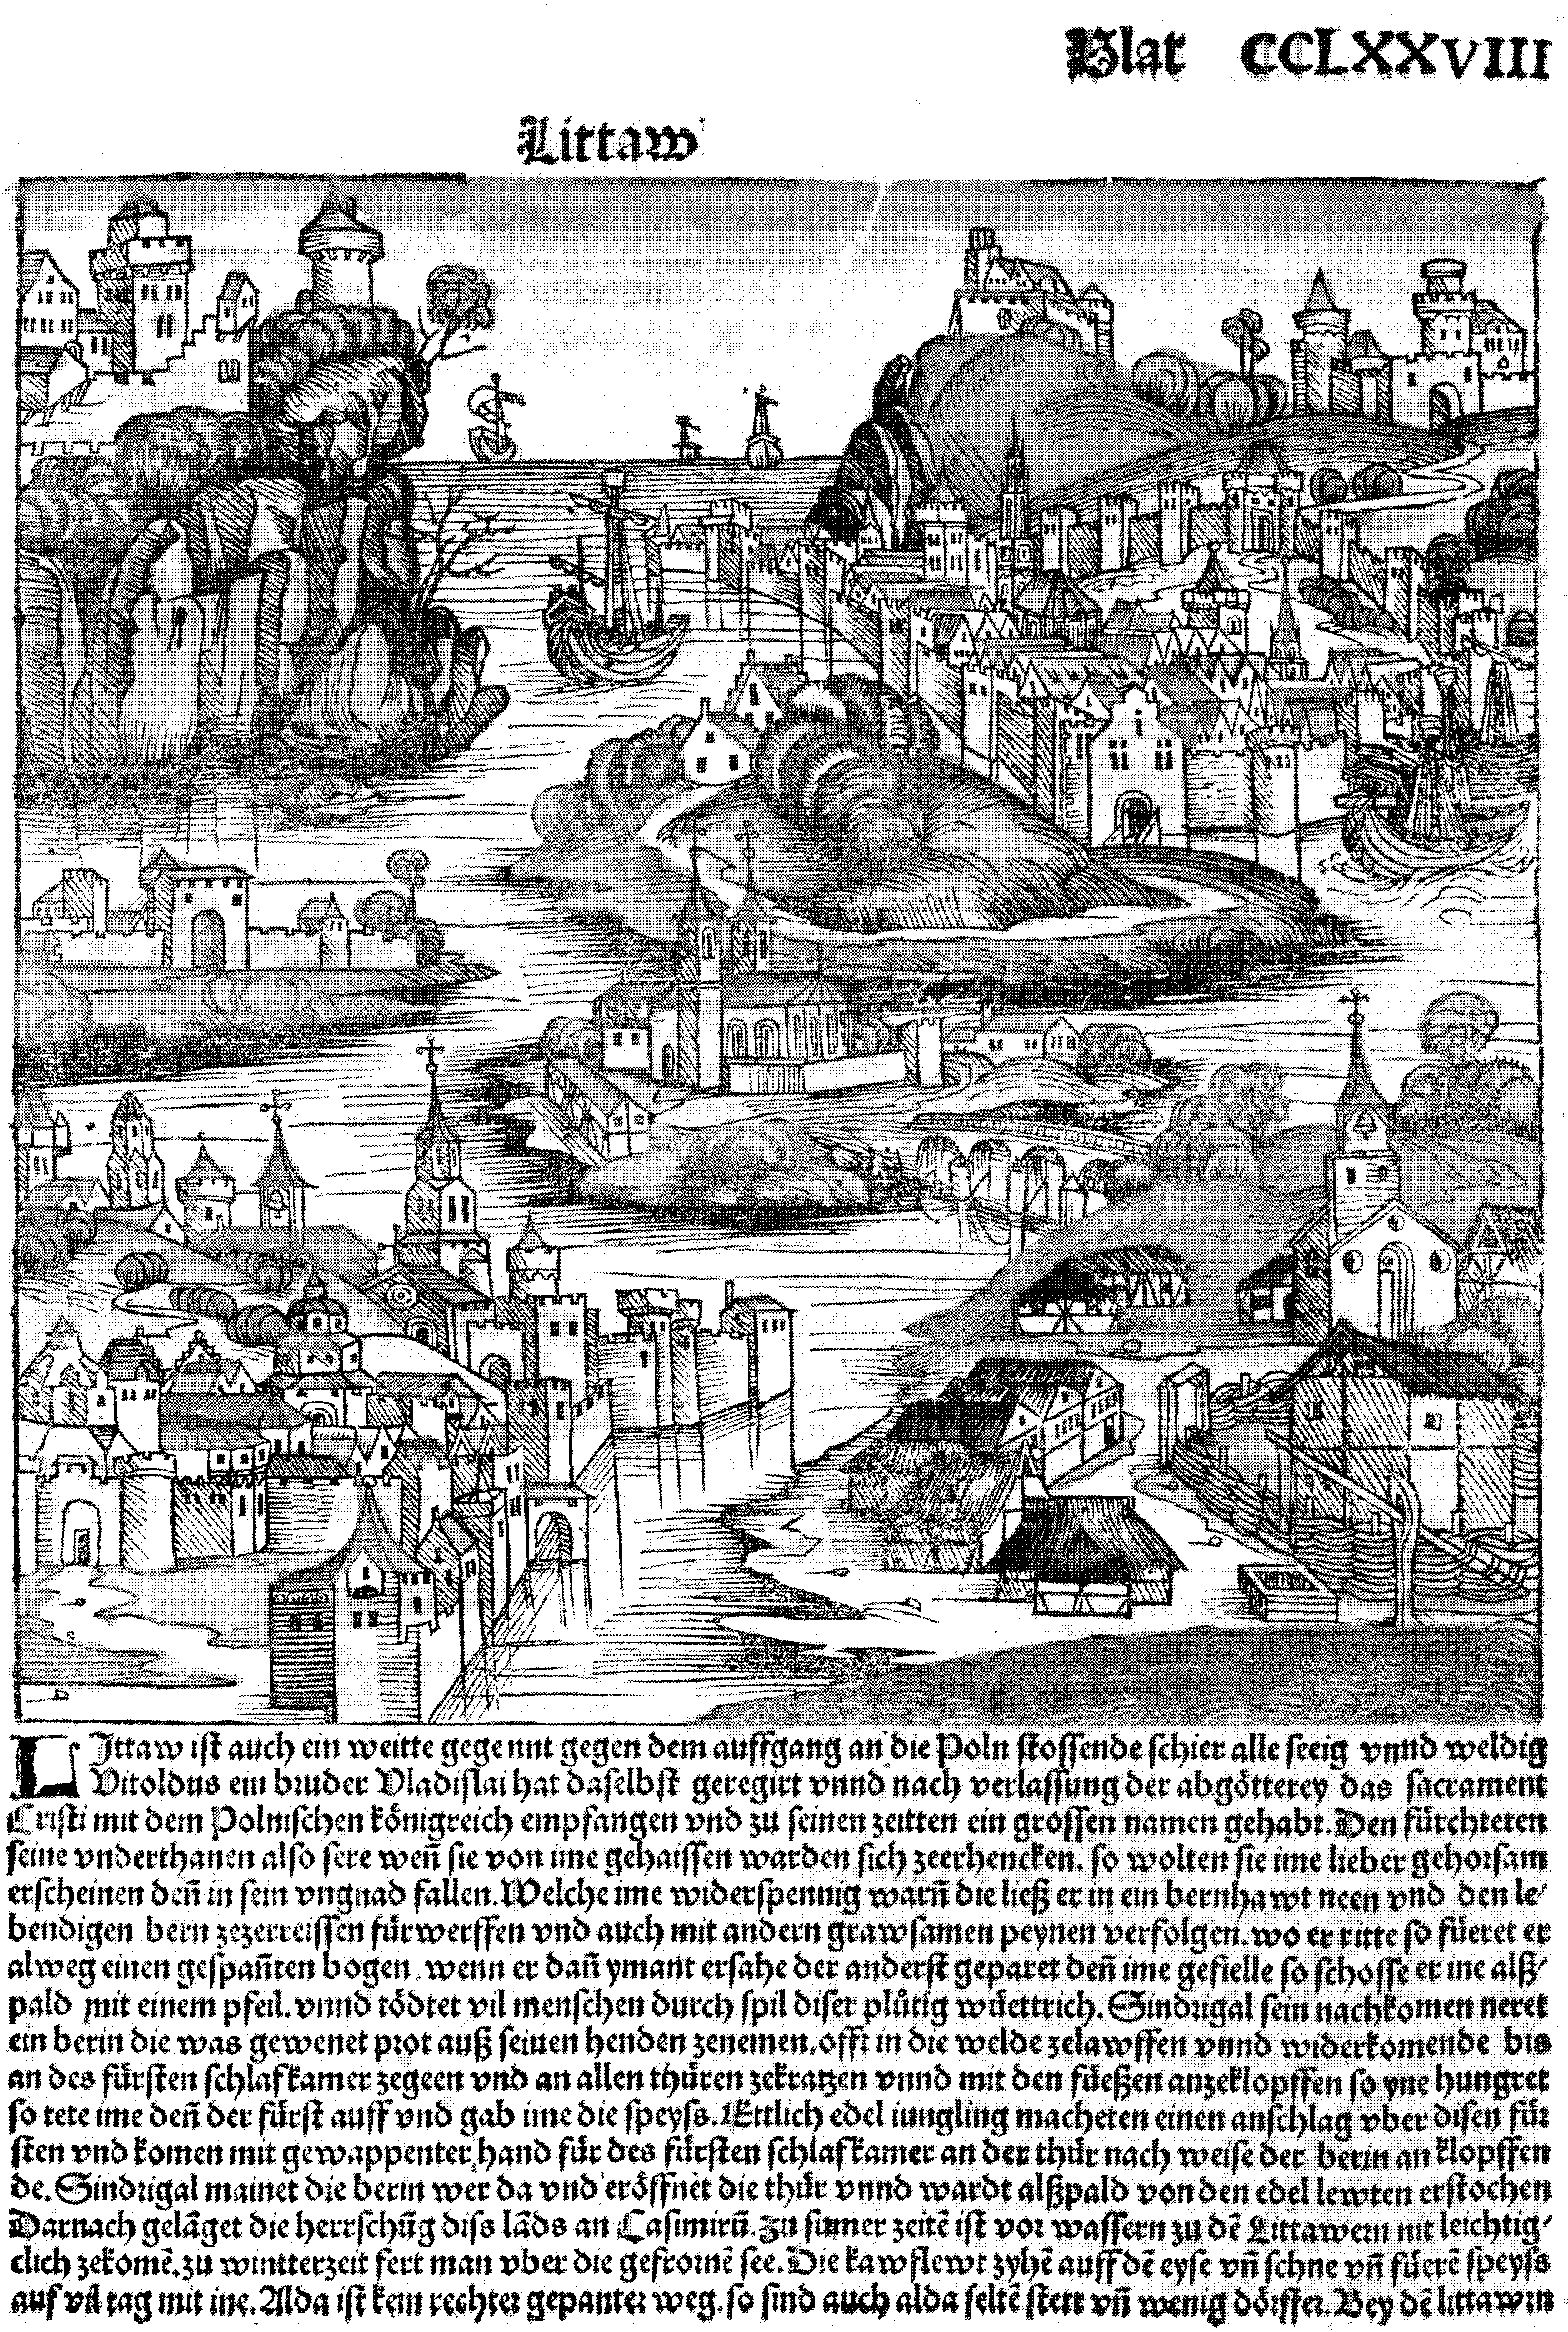
\includegraphics[width=10cm]{./ilustra-04.png} \footnotesize Lituânia (ou \textit{Littaw}), um retrato de um país em \textit{Crônica de Nuremberg}, 1493.}
% \end{center}

%Lithuania is mostly flat and lacks navigable waterways, and at the time, was sparsely populated with modest settlements almost entirely built out of wood. Hence, the image is a pictorial misconstruction of reality, a marker of Lithuania’s distance from the European centres of geographical explorations. Still, the accompanying description gives Lithuania a commanding role in the constitutive matters of Europe placing it alongside such countries as France, England, Spain and Portugal. 

\begin{figure}[!hp]
    \centering
    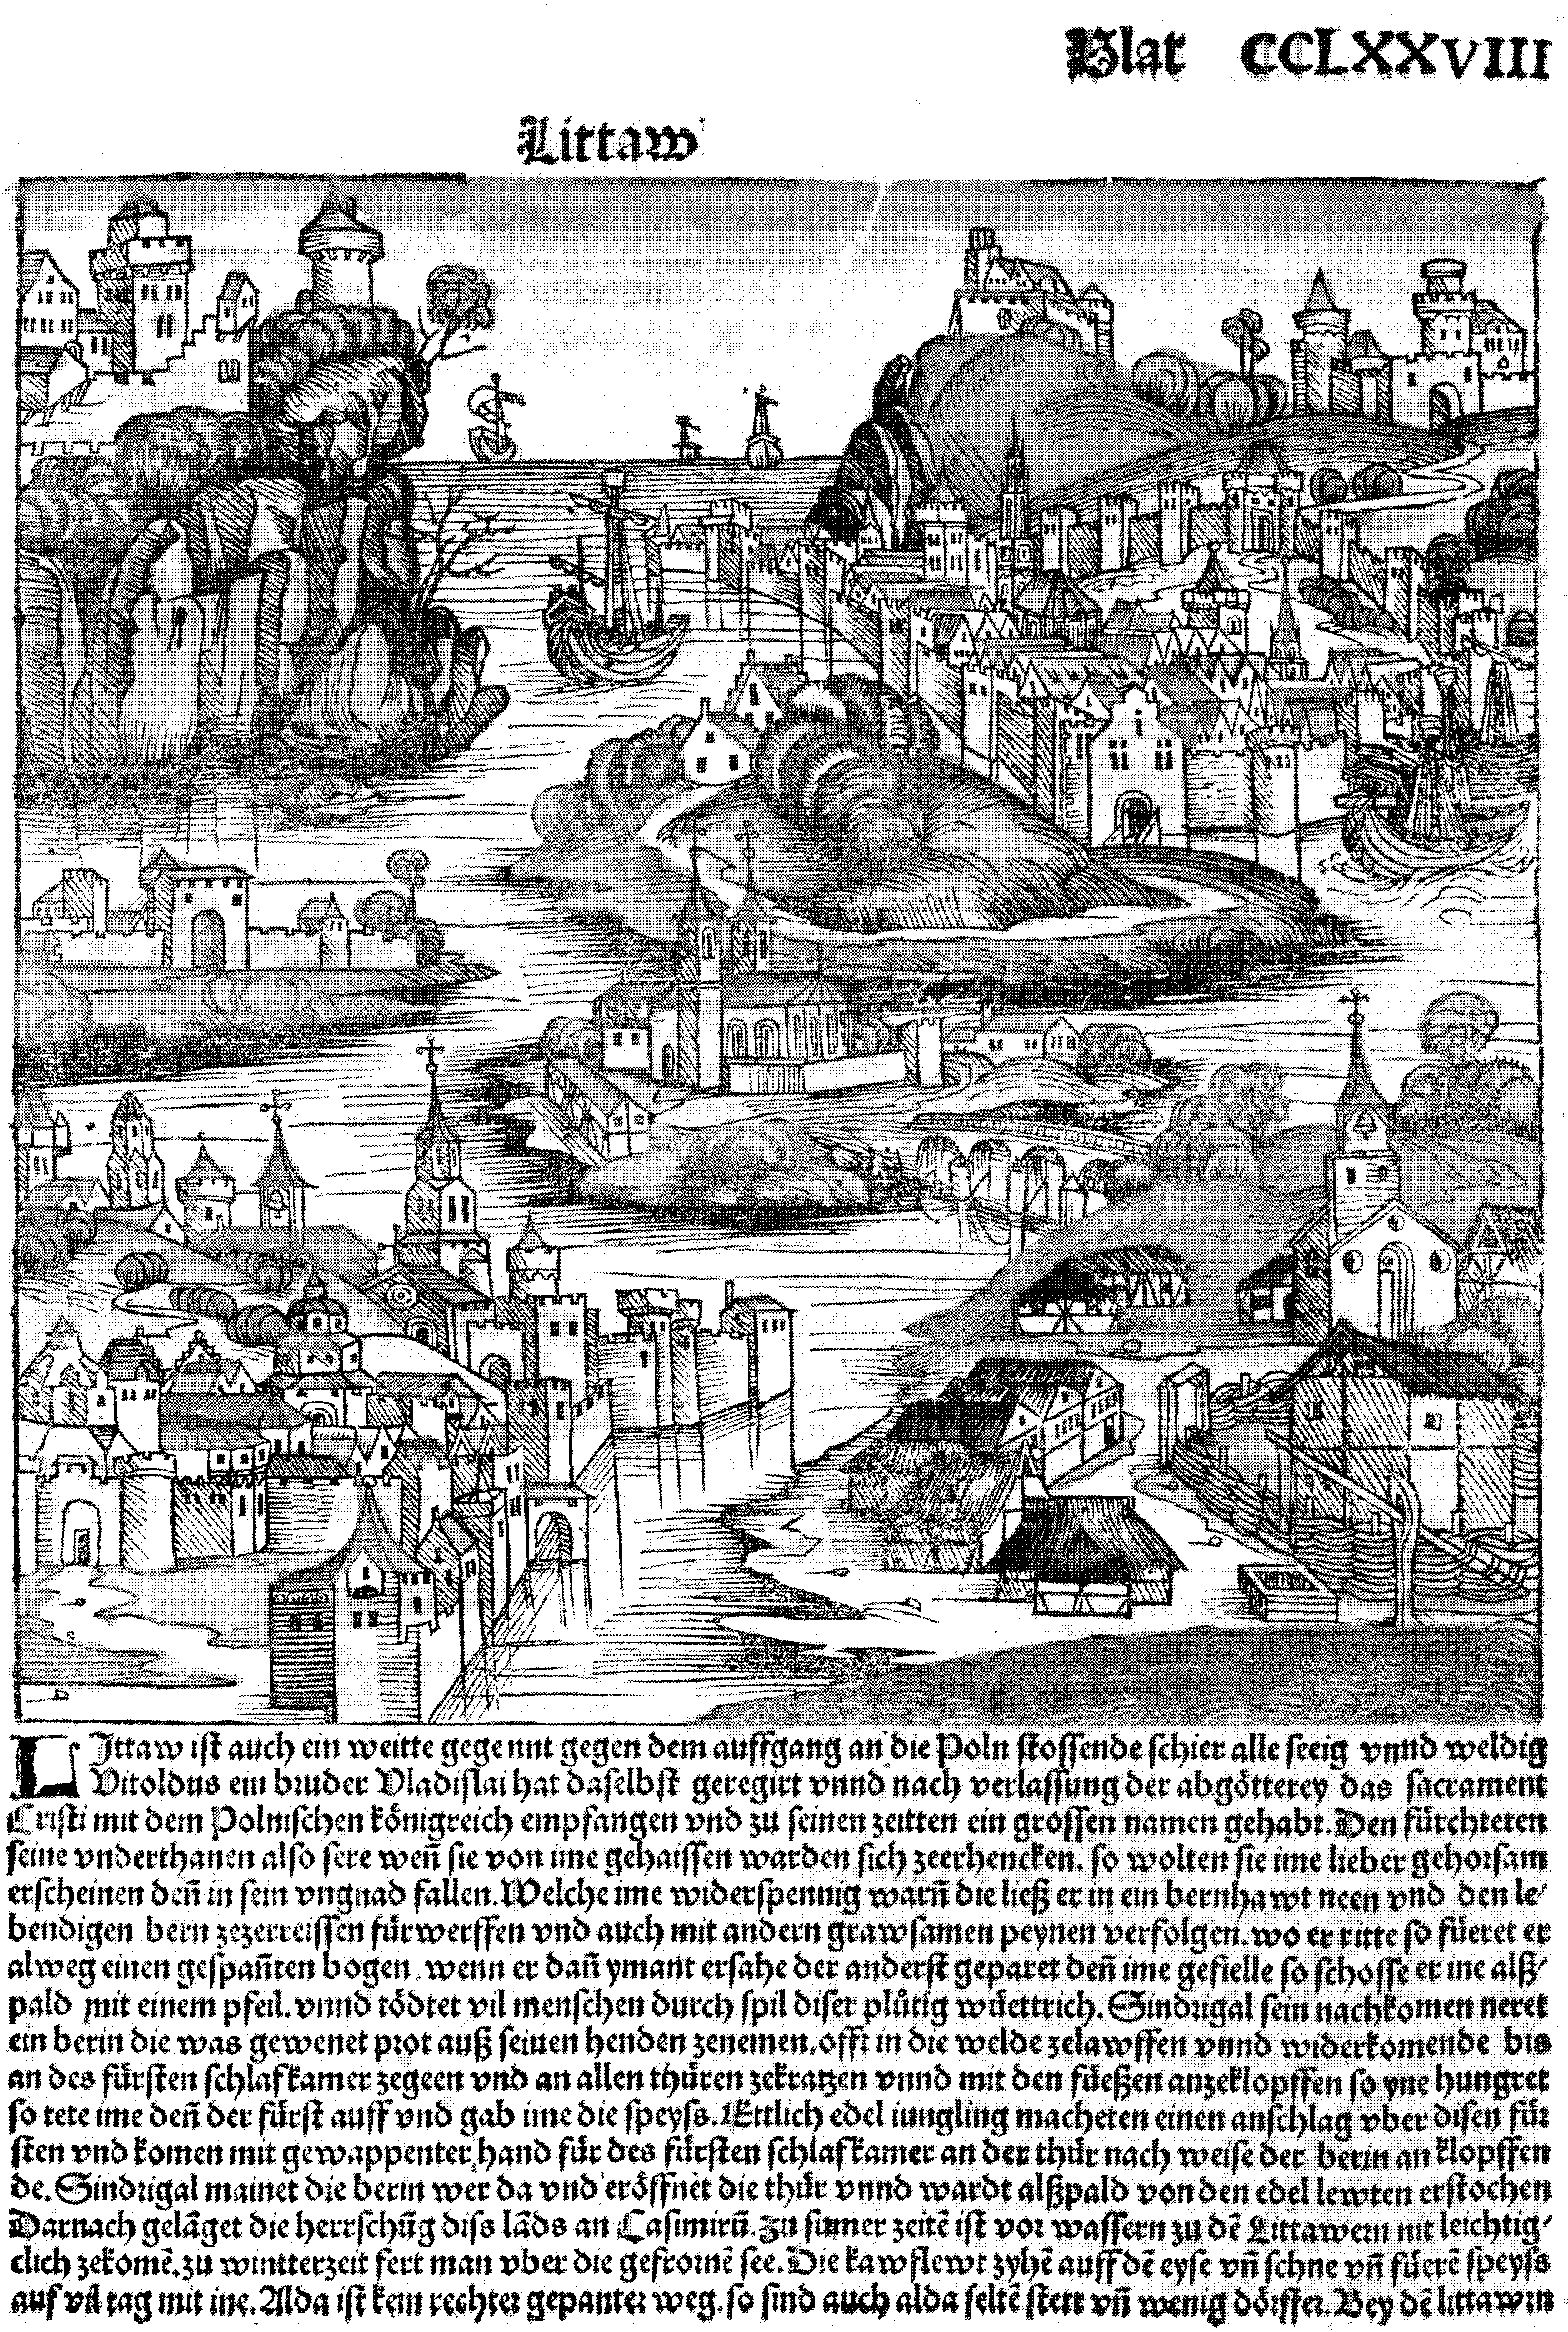
\includegraphics[width=\textwidth]{ilustra-04.png}
    \caption{Lituânia (ou \textit{Littaw}), retrato de um país em \textit{Crônica de Nurembergue}, 1493.}
\end{figure}


Ferreri, católico fervoroso, teve mais sucesso em convencer o rei
polonês a lutar contra a crescente onda de pensamento protestante. Na
Polônia, ele organizou um auto"-da"-fé público com os livros de Lutero (um
dos primeiros eventos dessa natureza na Europa) e incentivou a
ratificação de um édito banindo as publicações luteranas. Ofuscado pelo
êxito inicial, o núncio instigou uma campanha inflamada contra os fiéis
ortodoxos, que constituíam maioria da população lituana. Nessa guerra
teológica de duas frentes, Ferreri encontrou um cúmplice cuja estória de
vida o levou a Vilna. Durante algum tempo, a chancelaria papal em Roma
vinha recebendo solicitações das mais altas autoridades clericais e
seculares da Polônia"-Lituânia a fim de iniciar o processo de canonização
do Príncipe Casimiro, irmão mais velho de Alexandre e Sigismundo. O Papa
Leão \versal{x} levou o pedido a sério e instruiu Ferreri a coletar material e
dados testemunhais relativos aos feitos santos do falecido príncipe.

Casimiro era neto de Jogaila, quarta geração a partir de Gediminas.
Nasceu em 1458 como segundo filho do rei, e foi criado para governar.
Depois que o irmão mais velho assumiu o trono da Boêmia, Casimiro, então
com treze anos, foi enviado por seu pai à Hungria para reivindicar o
título real daquele país. A guerra rapidamente azedou: as tropas
mercenárias, sem soldo e desmoralizadas, desertaram, deixando em
desgraça o jovem e desamparado pretendente ao trono. Humilhado pelo
fracasso, Casimiro voltou transformado da guerra. Passou a rejeitar o
luxo e as facilidades da vida na corte, devotou sua energia juvenil ao
celibato e ascetismo, e concentrou sua atenção de príncipe à caridade e
ao trabalho evangélico. Apesar da perturbadora piedade e da saúde
precária do príncipe (que sofria de tuberculose), o pai de Casimiro o
escolheu como sucessor ao trono polonês. Com o estímulo paterno,
Casimiro se tornou um ativo governante da Polônia e, durante suas
costumeiras visitas à Lituânia, apelava a seu pai para fortalecer a
igreja católica na região por meio de restrições à liberdade religiosa
da população ortodoxa. Embora contrariasse os planos da família, o
príncipe se recusou a desposar a filha do imperador do Sacro Império
Romano Germânico. Corria o boato de que Casimiro, em sua beleza
angelical, passava as noites orando, rejeitando por completo o sexo e a
procriação, mesmo como obrigação familiar ou real. Quando os médicos,
com o consentimento dos pais, prescreveram"-lhe sexo com uma bela mulher
como o mais eficaz antídoto para sua condição de tuberculoso (e
presumidamente impotente), ele declarou preferir a morte e a celestial
vida no além aos prazeres fortificantes de ato tão pecaminoso. Foi
encontrado morto, em posição de prece, na gélida manhã de 4 de março de
1484, aos vinte e seis anos de idade, no umbral da entrada de uma igreja
numa cidade lituana. Seu corpo foi levado até Vilna e sepultado na
cripta real da catedral.

Gestos piedosos e uma vida em celibato não eram suficientes para fazer
de Casimiro um santo. Eram necessários milagres para uma canonização
exitosa, de maneira que Ferreri foi atrás deles em Vilna. Ao longo de
uma viagem de um mês desde a Polônia até Vilna (que, de acordo com
alguns de seus contemporâneos, se localizava bem perto do Polo Norte),
Ferreri foi se conscientizando cada vez mais da orientação celestial de
Casimiro. Durante toda a viagem, chuvas torrenciais caíram violentamente
sobre a terra, com tempestades e trovões que anunciavam o iminente fim
do mundo. O núncio, entretanto, não foi atingido por uma única gota. O
dilúvio diário só começava à noite ou tão logo os viajantes encontravam
refúgio. De fato, o mau tempo, nas palavras do núncio, facilitou a
viagem, pois ``durante o dia, as nuvens nos protegiam do sol escaldante.
E as chuvas noturnas nos pareciam uma bênção celestial, pois lavavam a
poeira (que torna aqui as viagens tão torturantes) das estradas de
terra, de maneira que ela era incapaz de molestar nossos olhos.
Surpresos por nossa boa sorte, compreendemos que tudo aquilo era
recompensa de Deus pelo nosso trabalho de pesquisa dos feitos do Bendito
Casimiro, cuja história de vida santa passou a habitar amorosamente os
nossos corações.''\footnote{Zacharias Ferrerius, Vita \textsc{s}.\,Casimiri, em Mintautas Čiurinskas, \textit{Ankstyvieji \textsc{šv}.\,Kazimiero gyvenimai}. Vilna: Aidai, 2004, p. 75.}
O drama atmosférico alcançou o ápice diante dos portões de Vilna, onde,
após ``viajar pela floresta primeva, desabitada e cheia de pântanos,'' o
núncio foi recebido por uma imensa multidão. Ao término da missa de ação
de graças e da ceia, Ferreri, ``hospitaleiramente acompanhado pelos
bispos de Vilna, Kiev e Kaffa, magistrados, clérigos e inúmeros fiéis
católicos e cismáticos (ortodoxos)'', estava pronto para entrar na
cidade. Mais uma vez, os céus assumiram uma coloração ameaçadora. Uma
tormenta ecoou à distância. Os patrícios, todos envergando ``sedas,
pedras preciosas e ouro'', e um incalculável número de plebeus fitaram
nervosos o céu. Fortuitamente, a tempestade eclodiu só depois da
procissão cerimonial, que terminou junto ao altar central da catedral.
Para Ferreri, aquilo havia sido sinal indubitável da imaculada santidade
de Casimiro.\footnote{Ibid., p. 79.}

Ferreri deve ter ouvido falar da visita de outro emissário papal,
Jacobus Piso da Transilvânia, que havia passado pela cidade seis anos
antes, em 1514. Piso tinha viajado a Vilna para celebrar a mais recente
vitória polono"-lituana sobre um exército russo em Orsha. Essa derrota de
Moscou não havia sido atribuída a quaisquer intervenções divinas: a
honra da vitória fora repartida entre o hetman\footnote{Título do segundo mais alto comandante militar, depois do monarca, usado do século \textsc{xv} ao \textsc{xviii} na Polônia e na Lituânia. [N.\,E.]} do exército lituano e o
rei da Polônia, irmão de Casimiro. Piso permanecera cinco dias em Vilna,
onde escreveu um poema de dezesseis versos, intitulado ``De Lithuania'',
publicado em 1533 em Viena, descrevendo cada dia de sua visita. No
primeiro dia, o viajante exausto, causticado pelo calor, foi revigorado
pelas águas refrescantes de Vilna. No dia seguinte, ele presta homenagem
ao hetman e, um dia mais tarde, a notícia da vitória é publicamente
confirmada. No quarto dia, confirma ``a glória do rei'' ao observar a
procissão de inimigos capturados. Finalmente, no quinto dia, ``chegou o
feliz momento'' em que o gracioso rei permite ao cansado diplomata
deixar a cidade. ``Que mais haveria a dizer?'' Piso conclui o poema,
respondendo a sua própria pergunta retórica: ``Adeus, terra dos
lituanos, e seja forte, pois não gostaria de morar aqui, mesmo que fosse
tratado como um deus.''\footnote{Jacobus Piso, ``De Lithuania'', em Eugenija Ulčinaitė, \textit{Gratulatio Vilne}. Vilna: Lietuvių literatūros ir tautosakos institutas, 2001, p. 27.}
A experiência de Ferreri em Vilna foi diferente. Ele foi tratado, se não
como um deus, ao menos como um reverenciado mensageiro do Santo Padre.
Permaneceu por seis meses na cidade, de setembro a fevereiro, e apreciou
sobremaneira o caráter social e cerimonial da visita. Ferreri aproveitou
vigorosamente de seu alto estatuto eclesiástico, convocando um sínodo e
protestando contra novas e velhas heresias: os ensinamentos de Lutero e
a pregação ortodoxa russa. O frio do inverno, contudo, ameaçou destruir
seu trabalho espiritual. Pois para os italianos, segundo Ferreri,
``acostumados ao clima romano, mesmo um frio ameno pode ser um perigo.''
Mas na ``Lituânia, que é um país ártico onde até animais silvestres
morrem congelados, e árvores e casas feitas de troncos racham de tanto
frio'', pode"-se facilmente contrair queimaduras de frio e morrer rápido.
Mas o Todo"-Poderoso mostrou sua misericórdia; aquele inverno foi o mais
brando de que se teve notícia. No Natal, os italianos puderam ficar do
lado de fora toda a noite e todo o dia, indo de igreja em igreja
enquanto ``pregavam contra as heresias dos russos,'' sem qualquer dano a
suas sensíveis disposições. E enquanto Ferreri agradecia a Casimiro pelo
tempo agradável, ``os lituanos eram unânimes quanto ao fato de que só
nós, italianos, podíamos ter trazido o calor de Roma'' para
Vilna.\footnote{Zacharias Ferrerius, op. cit., p. 81.}

Os habitantes locais foram eficazes em revelar as intervenções
miraculosas de Casimiro vividas por eles. Devotos surdos, cegos,
aleijados e doentes eram rotineiramente curados de suas condições no
local de sua sepultura. Uma menina ressuscitou da morte. De fato,
considerava"-se que o futuro de todo o país estivesse nas mãos do
príncipe defunto. Contaram a Ferreri que, um ano antes, um milagre,
``raramente conhecido no passado e jamais visto em nossa era,'' havia
salvado a Lituânia da aniquilação completa. Tropas da Moscóvia ---
contando sessenta mil soldados --- invadiram a Lituânia, que só conseguira
reunir uma força de dois mil voluntários. Toda esperança estava perdida.
Vilna ficou desprotegida, seus habitantes prontos para morrer ou viver
no cativeiro. Com lágrimas nos olhos, os soldados lituanos suplicaram a
Casimiro por proteção e perdão por não o venerarem como santo. Sua
coragem foi recuperada pela prece e, ``amparados pela fé'', atacaram
indômitos o inimigo. Os lituanos venceram a batalha sem perder um único
homem.\footnote{Ibid., p. 69.}

%{[}figura 10{]}
%
%São Casimiro, 1749. Esta imagem iconográfica do santo o retrata diante
%de três símbolos de Vilna: a Capela de Casimiro na catedral, a Colina do
%Castelo e a Colina das Três Cruzes.

Ferreri coletou meticulosamente diversos testemunhos sobre os milagres,
incluindo seus próprios relatos das ``abençoadas'' condições climáticas,
completando assim a primeira hagiografia de Casimiro enquanto ainda em
Vilna. O livro, \textit{Vita \textsc{s}.\,Casimiri}, publicado em 1521, descreve a
vida do santo sob um crivo humanista, entrelaçando o \textit{curriculum
vitae} miraculoso de Casimiro a descrições mais mundanas da família
real, da história nacional, de fatos geográficos e detalhes
etnográficos. Embora Vilna já houvesse dado ao mundo três mártires
santos, eles foram rejeitados como hereges pela igreja católica. Em
1347, três membros da corte ducal, que haviam se convertido à fé
bizantina ortodoxa, foram torturados e assassinados por uma multidão
pagã em Vilna. Trinta anos mais tarde, as relíquias foram levadas até
Hagia Sophia em Constantinopla, a igreja patriarcal do Império
Bizantino. A veneração dos três mártires sobreviveu à conquista otomana
de Constantinopla e foi fortalecida pelo Metropolita de Moscou, que, em
1549, adicionou"-os à lista universal dos santos ortodoxos russos. Essa
hagiologia ortodoxa fez de Vilna parte do mundo bizantino, e Ferreri
estava determinado a tornar esse fato irrelevante ao santificar Casimiro
como progenitura do universo latino.

No livro, o núncio procurou estabelecer uma conexão familiar entre Vilna
e Roma ao indicar uma similaridade ortográfica entre os nomes Lituânia e
Itália\footnote{\textit{Lituânia} e \textit{Itália}, respectivamente}. Na verdade,
ele amalgamou ambos os nomes em \textit{Litaliania}, um ilustre país
completamente imaginário, cujo ``antigo passado se baseia nas antigas
colônias estabelecidas pelos colaboradores do grande Pompeu.''\footnote{Ibid.,
  p. 51.} Apesar da afiliação genealógica, a Lituânia, ``país de frio
pungente, onde o verão é raro visitante'', era a antítese da Itália. Ao
invés de ser abrigada pelo Mediterrâneo e pelos Alpes, a Lituânia é
``rodeada por todos os lados por vastas planícies cobertas de florestas
e repletas de lagos e pântanos.'' Não há ``vinhedos ou pomares'', mas a
floresta é habitada por ``inúmeros animaizinhos apreciados pela pele
quente e luxuosa.''\footnote{Ibid., p. 75.} Ademais, ao misturar Itália
com Lituânia, Ferreri colocou Vilna no mapa renascentista do mundo da
antiguidade. Como a antiga Roma, a Vilna renascentista se encontra na
encruzilhada de diversos caminhos comerciais que transportam riqueza
``dos mares Alemão {[}do Norte{]}, Sarmácio {[}Báltico{]} e Pôntico
{[}Negro{]} e mesmo de algumas terras mais remotas --- Armênia, Cítia,
Trácia, Grécia e Mísia {[}Ásia Menor{]}.''\footnote{Ibid.}

Ferreri elogia Casimiro como a corporificação da antiga unidade entre a
Lituânia e a Itália, concluindo a hagiografia com uma celebração de
Vilna como cidade destinada a se tornar o luzeiro da solidariedade
cristã:

\begin{quote}
Rejubile"-se, gloriosa e bela Itália, por ter produzido as honrosas
nobrezas italianas e lituanas, que nos deram Casimiro. Rejubile"-se,
vasta e espaciosa Sarmácia, por ter conquistado o gelo, o frio e sua
própria nudez enquanto nutria essa belíssima e bem"-aventurada árvore da
vida, gerando o mais doce fruto de honra e virtude. Rejubile"-se, santa e
pia Igreja Mãe, por dar à luz Casimiro como filho legítimo de Cristo e
guerreiro da fé\ldots{} Sobretudo, rejubile"-se, Vilna --- cidade gloriosa,
onde os ossos brancos de Casimiro, seu amado corpo e santas relíquias
serão conservados para os pósteros como garantia de sua glória e
imortalidade. Partilhemos destas novas com cada igreja cristã e que o
nome de Deus seja louvado em todos os templos com música: aqui com
canções, acolá com hinos de órgão!''\footnote{Ibid., pp. 83--85.}
\end{quote}

A saudação laudativa a Casimiro veio um século mais cedo. O Vaticano não
encontrou falhas na vida santa de Casimiro, mas o Papa Leão \versal{x} morreu em
1521 e, logo após seu retorno da Lituânia, Ferreri também faleceu. O
saque de Roma por parte das tropas imperiais em 1527 e as arrebatadas
controvérsias religiosas na Europa deixaram por muito tempo em suspenso
a beatificação do piedoso príncipe sarmácio. De maneira que, enquanto a
doutrina protestante fervorosamente expurgava o Céu e a Terra da
veneração idólatra, a Vilna católica, por enquanto, ficara sem
padroeiro.

%{[}figura 11{]}
%
%``Sarmácia, província limiar da Europa'', em \textit{La cosmographie
%universelle}, 1572.

\chapter{Mapeando a Sarmácia}

%\setlength{\epigraphwidth}{.45\textwidth}
\begin{epigraphs} 
\qitem{Enquanto a moldura cartográfica em que os homens {[}renascentistas{]}
podiam pensar sobre si mesmos como europeus se definia cada vez melhor,
e quando as pessoas de um país passaram a saber mais sobre as pessoas de
outros países através de viagens e leituras crescentes, uma
contra"-tendência se fez presente: saber não necessariamente significava
gostar. A informação abria as mentes; mas também alimentava
preconceitos.}{\textsc{john hale}}
\end{epigraphs}

Um dos primeiros mapeamentos de Vilna de que se tem conhecimento foi
realizado em 1513 num mapa intitulado \textit{Tabula moderna Sarmatie
Europa}, publicado em Estrasburgo.\footnote{Aldona Bieliūnienė et all, \textit{Lithuania on the Map}. Vilna: Lietuvos nacionalinis muziejus, 1999, pp. 24--25.} Segundo a legenda cartográfica, o mapa era produto da revisão de um mapa anterior, feito por Nicolaus Cusanus
(1401--1464), cardeal e governador de Roma, que tentou introduzir o
antigo conhecimento geográfico no terreno político da Europa do século
\textsc{xv}. O Grão"-Ducado da Lituânia surge, pela primeira vez (até onde se tem
notícia), na versão de 1491 do mapa de Cusanus; sua capital, porém, é
indicada apenas por uma cidade anônima. Na versão de 1513, a demarcação
do território da Lituânia é borrifada por diversas cidades nomeadas e
bem indicadas. Ironicamente, dessa vez o cartógrafo tanto se
entusiasmara em popular a Lituânia com numerosas cidades e castelos, que
acabou registrando Vilna duas vezes no mesmo mapa. A primeira legenda
identifica corretamente a capital lituana como a cidade de \textit{Wilno},
situando"-a na confluência de dois rios anônimos. A segunda legenda marca
a cidade de maneira incorreta como \textit{Bilde}, localizando"-a ao sul da
Wilno original. O nome \textit{Bilde}, que não tem equivalente histórico
conhecido, parece ser corruptela do topônimo \textit{Wilde}, que foi usado
para identificar Vilna em diversas descrições da Lituânia, em alemão, ao
longo do século \textsc{xv}. O uso alemão de \textit{Wilde} para o nome de Vilna\footnote{Como em
\textit{die statt} Wilde\textit{, für die Wilde, zur} Wilde.} tem sua origem nas
antigas crônicas da Ordem Teutônica, mas continuou sendo empregado
esporadicamente em diversos registros e mapas até o século \textsc{xviii}.\footnote{A respeito das variações históricas do nome \textit{Vilnius}, ver Jonas Jurkštas, \textit{Vilniaus vietovardžiai}. Vilna: Mokslas, 1985. E também Aleksandras Vanagas, ``Miesto vardas Vilnius'' em \textit{Gimtasis žodis}, n. 11, novembro de 1993.}
Imprecisões geográficas não eram incomuns nas primeiras crônicas
europeias e, no ambiente fronteiriço da Lituânia, nomes vernaculares
estavam sujeitos a uma grande variedade de erros de pronúncia e
alterações linguísticas. Embora a afinidade ortográfica entre
\textit{Wilde} e \textit{Wilna} (ou \textit{Vilnius}) tenha provavelmente a ver com a
batalha ideológica e, neste caso, geo"-religiosa pelo controle da
Lituânia. A palavra alemã \textit{Wilde} tem conotações muito específicas:
\textit{der/\,die Wilde} significa selvagem. O vasto território coberto por
florestas que separava Vilna dos domínios dos cavaleiros teutônicos na
Prússia se mantinha despopulado devido aos incessantes ataques dos
cruzados e, em alemão, ele era simplesmente mencionado como \textit{die
Wildnis} --- o deserto. Isso tornou a ideia e a prática da \textit{reysa}
anual à Lituânia inseparável da experiência do país como última
fronteira do mundo conhecido.

Na Lituânia, a íntima relação entre o urbano e o selvagem --- cultura e
natureza --- atingiu um nível raramente encontrado na Europa Ocidental,
onde as cidades eram mais parte de um meio rural (e não florestal).
Mesmo após o fim dos ataques teutônicos, chegar até Vilna envolvia
inevitavelmente atravessar longas faixas desertas, onde perigos e
surpresas pululavam a cada canto. Eis a descrição de uma cosmografia do
fim do século \textsc{xv}:

\begin{quote}
\ldots{} a famosa floresta {[}que{]} cobre a Sarmácia nada {[}tem{]} de igual
em toda a Europa. A floresta se estende até Cracóvia {[}capital da
Polônia{]}, e é possível caminhar por ela até a Lituânia e a Cítia. Essa
enorme floresta abarca toda a região como braços esticados protegendo
grandes rebanhos de animais silvestres. Na parte setentrional da
floresta vivem ferozes bisões, bestas gigantescas que detestam a
presença humana; sua carne é bastante saborosa, a cor de sua pele se
assemelha ao limão; a cabeça é branca com chifres protuberantes; para
caçá"-los é necessário grande esforço.\footnote{Hartmann Schedel, ``Sarmatia'', capítulo de \textit{Liber chronicarum} impresso em Nurembergue por Anton Koberger em 1493, traduzido e editado por \textsc{b}.\,Deresiewicz. Londres: Oficyna Stanisław Gliwa, 1973, p. 86.} 
\end{quote}

Da perspectiva de qualquer aventureiro europeu, corajoso o suficiente
para adentrar nessa vastidão deserta do norte, Vilna deveria parecer uma
minúscula ilha urbana perdida no meio de um oceano de vegetação infinda.
Mas Vilna, com suas casas feitas só de madeira, não era apenas engolida
pela floresta; ela cresceu a partir dela. A cidade, à diferença de suas
primas europeias ocidentais, não existia em oposição à vastidão deserta,
mas se relacionava numa simbiose com ela.

Essa percepção foi sem dúvida incrementada pelas crenças e práticas
religiosas da população pagã local, que venerava fenômenos naturais tais
como o sol, a lua, o trovão, animais e sobretudo árvores e florestas. O
mais importante templo lituano pagão se localizava no coração histórico
de Vilna --- na confluência dos rios Neris e Vilnia --- e era protegido por
um arvoredo sagrado de carvalhos. O oxímoro de chamar uma cidade de
\textit{Wilde} posicionava"-a fora da Europa cristã urbana, onde a
fronteira entre os reinos natural e civil estavam mais claramente
definidos, quando não sempre marcados por uma muralha de pedra.
Portanto, não deveria nos surpreender tanto que Vilna tenha se tornado
europeia (ou seja, católica e latina) com a ajuda da lâmina de um
machado. O batismo da Lituânia em 1387 foi consagrado pela destruição
formal do arvoredo sagrado de carvalhos, que ficava no vale sacro aos
pés da colina do castelo. Na clareira que sobrou depois do expurgo
espiritual, a primeira catedral católica de Vilna --- uma construção em
pedra --- foi erguida.

Durante o Renascimento, o relativo isolamento geográfico de Vilna se
transformou em sua maior virtude do ponto de vista cultural. Localizada
nos limites de todos os ambientes espirituais da Europa --- católico,
protestante, bizantino ortodoxo, judaico, islâmico e mesmo pagão ---, a
cidade alimentava uma paisagem de tolerância religiosa e polinização
cultural cruzada. O pensamento humanista e a estética renascentista
chegaram a Vilna relativamente tarde. O estilo gótico alcançou seu
apogeu em Vilna só com a construção da elegante igreja de Santa Ana no
ano de 1500, quando o século da Renascença já estava despontando mais ao
sul. A primeira tipografia da cidade foi criada apenas em 1522, quase
setenta anos depois do primeiro livro impresso por Gutenberg em Mainz.
Mas o primeiro livro publicado em Vilna foi \textit{Um pequeno livro de
percurso}, uma coleção de hinos religiosos e um calendário da igreja
para os leigos da fé ortodoxa bizantina, ricamente impressa em cirílico
na língua eslava, antigo bielorrusso, pelo erudito humanista de educação
católica Francis Skaryna. Algumas décadas mais tarde, a tolerância
religiosa assumiu um caráter mais formal: em 1563, em meio a brutais
conflitos religiosos na Europa, uma lei garantindo liberdade religiosa
na Lituânia foi sancionada por uma assembleia de nobres em Vilna. No ano
seguinte, o grão"-duque editou um decreto proibindo as autoridades locais
de acusar os judeus de crime de assassinato ritual, a menos que se
baseassem no testemunho de três cristãos e três judeus. Tal equidade era
rara na Europa, onde a segregação religiosa era aplicada pela força
popular e frequentemente apoiada pela lei.

A corte ducal lituana, agora decisivamente instalada em Vilna, tornou"-se
ainda mais cosmopolita por meio de casamentos reais cristandade afora.
Diplomatas estrangeiros chegavam a Vilna não só para discutir questões
matrimoniais, como também para abordar questões de Guerra e paz. Em
1517, Sigismundo de Herberstein, um dos mais exitosos diplomatas do seu
tempo, passou pela cidade em seu trajeto rumo à Rússia a fim de negociar
uma trégua entre a Lituânia e Moscou, assinada finalmente em 1522.
Retornou à Lituânia em 1526 a fim de renovar o tratado. Herberstein
servia aos Habsburgos, a mais poderosa família governante da Europa, e
seu envolvimento pessoal no conflito russo"-lituano demonstra a crescente
importância geopolítica dos dois países (ainda periféricos) no contexto
do balanço de poder europeu. A Lituânia, país predominantemente ortodoxo
governado por uma família real católica, ocupava posição ímpar para
mediar os dois universos religiosos. Qualquer eventual aliança entre os
dois credos, e portanto a possibilidade de uma reunificação do mundo
cristão, teria que necessariamente passar pela Lituânia e sua capital,
Vilna.

Ao término da carreira diplomática, Herberstein publicou um livro,
\textit{Anotações sobre a Rússia}, que se transformou num tratado canônico
sobre a Rússia e países vizinhos. Dois capítulos tratavam da Lituânia:
um sobre geografia, história e natureza social do país; e o outro, nas
palavras do autor, se dedicava à pesquisa ``de seus animais selvagens.''
A descrição de Vilna feita por Herberstein deve ser lida à luz de sua
missão diplomática, que tentava estabelecer um terreno político, se não
cultural, comum entre Moscou e a Lituânia como o melhor garante de paz.

``Vilna,'' escreveu Herberstein, ``é rodeada por uma muralha, que
circunda vários templos e casas feitas de pedra. {[}\ldots{}{]} Ela
conta também com uma igreja paroquial e diversos mosteiros, entre eles o
Franciscano, construído a grandes custos e famoso pela estrita
disciplina. As igrejas russas ali são muito mais numerosas do que as que
foram erguidas para observar o ritual romano.''\footnote{Sigismund Herberstein, \textit{Notes upon Russia: being a translation of the earliest account of that country, entitled Rerum Moscoviticarum commentarii}, traduzido e editado por \textsc{r.\,h.} Major. Nova York: Burt Franklin, 1963, p. 87.} A poderosa milícia do grão"-duque ``enverga uma roupa comprida e porta arcos como os tártaros; mas têm também lança e
escudo, como os húngaros.''\footnote{Ibid., p. 86.} Do lado de fora da
cidade, ``as pessoas são miseráveis e terrivelmente oprimidas pela
servidão; pois quando qualquer homem que seja atendido por um grupo de
servos entra na casa de um lavrador, ele tem a liberdade de fazer,
impunemente, o que bem entender, levar ou consumir quaisquer víveres, e
mesmo surrar cruelmente o próprio lavrador.'' Ademais, a corrupção e a
servidão grassavam em todos os níveis sociais: ``os lavradores
absolutamente não têm qualquer acesso a seus senhores a não ser que
levem presentes e, caso sejam admitidos, serão encaminhados aos mordomos
e administradores, os quais, se não receberem presentes, não tomarão
providências, nem emitirão qualquer decisão favorável ao requerente. E
esse não é o caso só dos pobres, mas também dos nobres, sempre que
desejassem obter algum favor de seus superiores. Certa vez ouvi de um
jovial ministro de alta patente, próximo ao rei, de que a única palavra
na Lituânia é `ouro'.''\footnote{Ibid., p. 94.} Mais escandaloso ainda,
porém, era o que ocorria nas entranhas da floresta lituana, onde
``testemunham"-se por vezes coisas horrendas; pois nela habita um
considerável número de idólatras, que adoram, como uma espécie de deus
doméstico, uma espécie de réptil, que tem quatro pernas curtas como um
lagarto, e um corpo negro e inchado, que não ultrapassa três palmos de
comprimento.''\footnote{Ibid., p. 99.}

À época das diligências diplomáticas de Herberstein, o Grão"-Ducado da
Lituânia abarcava os territórios da atual Lituânia, Bielorússia, Ucrânia
e parte ocidental da Rússia. Ao norte, o Grão"-Ducado fazia fronteira com
novos bastiões do Luteranismo: a Suécia, a Prússia e a Livônia (atuais
Letônia e Estônia). A leste, os limites ducais chegavam tão longe quanto
os principados ortodoxos russos de Novgorod e Smolensk, bordejando o
estado de Moscou. Ao sul, ele criava uma imensa zona tampão com o mundo
otomano, com suas fronteiras voláteis com o Canato da Crimeia, governado
por muçulmanos, e com a Moldávia, dominada pela ortodoxia bizantina. O
país abrangia diversas divisões geográficas europeias: estendia"-se das
planícies repletas de bosques e pântanos da região do Mar Báltico até o
planalto de estepes virgens da costa setentrional do Mar Negro. Incluía
também a fértil área das encostas carpáticas da Volínia e Podólia, bem
como o território abundante em madeira da floresta russa.

Essas vastas terras eram habitadas por uma grande variedade de povos:
poloneses, lituanos, rutenos (ucranianos), bielorrussos, russos, judeus,
alemães, letões, armênios, tártaros e outros grupos minoritários. Seis
idiomas --- polonês, latim, bielorrusso antigo, hebraico, alemão e armênio ---
eram utilizados para propósitos jurídicos. A confissão religiosa era
igualmente diversa. Num nível básico, havia três grandes comunidades
cristãs no ducado: a católica, a greco"-ortodoxa e a protestante. Em
1596, adicionou"-se um quarto elemento --- a igreja greco"-católica, que
tentou resolver o cisma dogmático e litúrgico entre as igrejas grega e
latina. A maior parte dos judeus lituanos eram \textit{ashkenazi} (europeus
ocidentais) na origem, à exceção dos caraítas, que haviam sido trazidos
pelos grão"-duques nos séculos \textsc{xiv} e \textsc{xv} de sua Crimeia natal, às margens
do Mar Negro. Achava"-se que os caraítas descendessem dos cazares, povo
semi"-nômade que aceitara o judaísmo no século \textsc{ix}. Os judeus \textit{ashkenazi}
praticavam a forma rabínica do judaísmo, escreviam em hebraico e, na
maior parte das vezes, falavam iídiche vernacular; os caraítas seguiam a
versão babilônica da fé judaica, usavam o alfabeto árabe para as
escrituras hebraicas e falavam uma língua túrquica. Havia também
tártaros muçulmanos que, assim como os caraítas, vinham da Crimeia.

Era difícil para um estrangeiro compreender a vastidão e a
heterogeneidade culturais da Lituânia. Tudo ficava ainda mais confuso
graças à definição geográfica ambígua da Lituânia, que portava dois
significados espaciais: primeiro, como estado político do Grão"-Ducado da
Lituânia e, segundo, como antiga província pertencente ao patrimônio
original de Gediminas. Entre ambas as definições havia uma diferença de
proporções continentais. Em seu auge, na primeira metade do século \textsc{xvi}, o
Grão"-Ducado tinha basicamente o tamanho do Sacro Império Romano
Germânico e constituía o maior corpo político na Europa depois do estado
russo, que vinha se ampliando velozmente. Em contraste, a província (ou
país) da Lituânia, apenas parcialmente habitada por lituanos, cobria um
território muito menor que circundava Vilna. Para complicar as coisas, a
Lituânia (o Grão"-Ducado e a província) se aliava invariavelmente a seu
parceiro monárquico, a Polônia. Essa parceria política foi aprofundada
pela União de Lublin, que, em 1569, criou o estado combinado da
Polônia"-Lituânia ou, como ficou conhecido constitucionalmente, a
República das Duas Nações.

\asterisc

Nem a identidade ou nação polonesa nem a lituana era capaz de
corporificar com exatidão tal diversidade geográfica e cultural. O único
país que conseguia abranger essa união de diferenças era a ilusória
Sarmácia, cujas origens cartográficas podiam ser rastreadas nos
trabalhos históricos e geográficos dos antigos gregos e romanos.
Supõe"-se que o geógrafo Ptolomeu tenha situado a tribo bárbara dos
sarmácios em algum lugar das estepes entre os mares Azov e Cáspio. O
historiador Heródoto e outros comentadores deslocaram os semi"-nômades
sarmácios mais para o oeste, para a zona do Mar Negro e a bacia inferior
do rio Dnieper. Algum tempo depois, essa tribo de errantes eternos
deslocou"-se mais para o norte, para a região onde as vastas estepes e
planícies meridionais da Eurásia se encontram com as florestas e
pântanos setentrionais do litoral do Mar Báltico. Segundo o erudito
romano Tácito, aquela era uma área bravia próxima ao ``Mar Suábio''
(provavelmente o Mar Báltico), onde ``o nosso conhecimento do mundo
termina.''\footnote{Norman Davies, \textit{God's Playground: A History of Poland}, Vol. 1. Nova York: Columbia University Press, 1982, p. 45.} Pensadores e geógrafos renascentistas descobriram essa imperfeição no conhecimento espacial dos sábios antigos e a reproduziram
no mapa contemporâneo da Europa. O Mar Báltico se transformou em
\textit{Mare Sarmaticum} e as terras que se estendiam \textit{ad infinitum}
a sudeste daquele mar foram identificadas como Sarmácia, dividida em
duas áreas: \textit{Sarmácia europeia} e \textit{Sarmácia asiática}.

No início do Renascimento, a Sarmácia europeia foi descrita como ``uma
região extremamente vasta e deserta, selvagem e sem cultivo agrícola, de
clima rigoroso. Faz limite a leste com os moscovitas {[}Moscóvia{]} e o
rio Don; ao sul, com os dácios {[}Romênia{]} e panônios {[}húngaros{]};
a oeste, com boêmios, morávios, silésios e teutões; e ao norte com o Mar
Alemão {[}Báltico{]} e o porto de Gdansk.''\footnote{Schedel, op. cit., p. 85.} Essa vasta e confusa existência cartográfica da Sarmácia tornou"-se mais concreta com o surgimento do sarmacismo, ambiente
sócio"-cultural peculiar que encontrou terreno fértil entre a nobreza
polono"-lituana do século \textsc{xvi}.

O sarmacismo resultava de uma fusão de patriotismo regional com a
redescoberta dos textos clássicos romanos e gregos. Embora se baseasse
na geomitologia antiga, o sarmacismo ``era uma variação singular daquilo
que poderia se chamar auto"-definição nacional renascentista. No espírito
renascentista de um retorno às raízes, os povos da Europa procuravam ou
inventavam suas próprias origens míticas. O sarmacismo expressava para
os poloneses a ideia de que, assim como outras nações europeias, eles
também tinham origens nos povos abordados pelos autores da Antiguidade,
e seus ancestrais eram até mesmo mais velhos que os ancestrais de muitos
outros europeus.''\footnote{Thomas da Costa Kaufmann, \textit{Court, Cloister and City: The Art and Culture of Central Europe, 1450--1800}. Chicago: University of Chicago Press, 1995, p. 288.} Após a União de Lublin, o mito antiquado da Sarmácia facilmente englobou também a
Lituânia, tendo em vista que o perímetro cultural da identidade sarmácia ``foi gradualmente alterada a fim de incluir a nobreza não"-polonesa na
República. Todo nobre da República que defendesse as liberdades e
privilégios políticos de sua classe era considerado sarmácio. Com base
nesse mito ou ponto de vista, ergueu"-se uma doutrina que, no fim do
século \textsc{xvi}, constituía uma apologia ao \textit{status quo} político e
social.''

Por meio da invariável assimilação da classe alta
polono"-lituana, ``o sarmacismo se tornou, em sua essência, a
documentação `histórica' para a existência da nobreza e sua autoridade
política.''\footnote{Harry \textsc{e}.\,Dembkowski, \textit{The Union of Lublin: Polish Federalism in the Golden Age}. Boulder: East European Monographs, 1982, pp. 210--211.} A família real da linhagem de Jogaila era considerada a materialização da herança sarmácia: por exemplo, o
Grão"-Duque Alexandre (que residia em Vilna) era ``tido como o ornamento
da Sarmácia'' pois ``em toda a Sarmácia não há ninguém que se assemelhe
em coragem e mente tão sublime.''\footnote{Schedel, op. cit., p. 88.}

Uma das primeiras obras eruditas mais consistentes sobre a Sarmácia foi
escrita por Alexander Gwagnini (1538--1614), oficial italiano a serviço
do Grão"-Duque da Lituânia. Gwagnini se interessou pela história e
geografia da Lituânia e, em 1578, em Cracóvia, publicou um livro em
latim intitulado \textit{Sarmatiae Europeae Descriptio}. Em seguida, o
manuscrito foi republicado em várias edições diferentes e traduzido para
o polonês. Gwagnini igualou explicitamente a Sarmácia ao Grão"-Ducado da
Lituânia, que descreveu como um país ``muito expansivo'' com uma
``localização definida'' cobrindo ``vários ducados, estados e províncias
de nomes diferentes'' sob seu poder.\footnote{Alexander Gwagnini, conforme citado em Artūras Tereškinas, \textit{Imperfect Communities: Identity, Discourse and Nation in the Seventeenth"-Century Grand Duchy of Lithuania}. Vilna: Lietuvių literatūros ir tautosakos institutas, 2005, p. 237.}
Vilna, na época da União de Lublin, foi descrita como uma metrópole
caótica e agitada da fronteira sarmácia. A primeira visão panorâmica da
cidade, reproduzida na edição de 1576 de \textit{Civitates Orbis Terrarum}\footnote{Famoso atlas de cidades do mundo, criado pelo artista flamengo Franz Hogenberg e pelo cartógrafo Georg Braun, decano da catedral de Colônia.} 
dá a impressão de uma grande cidade construída quase exclusivamente de
madeira. A longa descrição da cidade resume o caráter exótico do lugar:

\begin{quote}
Vilna é uma cidade grande e densamente populada, centro do Grão"-Ducado
da Lituânia e da diocese. Chamada \textit{Wilenszki} pela população local,
e \textit{die Wilde} pelos alemães, ela toma o nome emprestado ao rio
local, que nasce na Lituânia e, depois de se unir ao rio Niemen, deságua
no \textit{Mare Prutenicum}, o mar Prússio. A cidade é circundada por uma
muralha de tijolo com diversos portões que nunca estão fechados.
[\ldots{}] A maior parte das casas é feita de madeira, pequenas e baixas,
desprovidas de dormitórios ou cozinhas, muitas vezes também sem
estábulos, embora vários residentes criem animais, construídas aqui e
ali de maneira caótica. Em algumas ruas, porém, como a Rua Alemã e a do
Castelo, alinham"-se belas casas de pedra, construídas por estrangeiros
vindos a negócio. Vilna tem dois palácios reais: um é grande e bonito,
com vários cômodos; o outro tem torres e se ergue sobre a colina. Embora
a Lituânia não tenha uma indústria mineira, há um arsenal de armas de
todo tipo na encosta da colina. As igrejas são em sua maioria feitas de
tijolo, mas há também algumas de madeira. Diferentes confissões têm suas
próprias casas de culto. Famoso por sua arquitetura de tijolo queimado,
o mosteiro Bernardino é o mais elegante. O Galpão Ruteno, onde se vendem
mercadorias vindas de Moscou, tais como as mais finas peles de lobo,
raposa branca, marta zibelina, arminho, leopardo e outros animais, é
fascinante também. Há inúmeros chafarizes nas ruas para uso dos
residentes, que estão todos conectados a uma fonte próxima ao Portão
Alemão.

Há diversos assentamentos extramuros, como em todas as cidades bem
concebidas, cada um com seu próprio nome. Um deles, engolfado pelo rio
Vilna, chama mais a atenção devido à sua pobreza. Como não há ruas,
casas minúsculas foram construídas sem qualquer sistema, como se
surgissem por mágica ou por acaso, norteadas apenas pela vontade de seus
bárbaros residentes. Quem quiser pode aparecer com algumas tábuas de
pinho e construir uma cabana primitiva. Longe do portão do palácio real,
o Rei Sigismund Augustus construiu em madeira um pavilhão de caça, onde
se abriga dos aborrecimentos e dissabores da vida urbana. O terreno do
pavilhão inclui um viveiro, num pequeno bosque cercado, destinado a
diversos animais caros e exóticos.

Os moradores de Vilna, em especial os que vivem nos casebres suburbanos,
não têm escola, são inativos, preguiçosos, indolentes, desprovidos de
qualquer conhecimento ou gosto pelas artes e ciências. São verdadeiros
escravos de seus senhores, sem qualquer desejo por liberdade.
Surpreendentemente, comprazem"-se em sua existência miserável e
demonstram amor e obediência apenas àqueles senhores que os repreendem e
açoitam inclementes. Enquanto isso, costumam fugir dos senhores que os
tratam bem.

A população não produz vinho, porém adora beber. Bebem hidromel e
cerveja, e especialmente apreciam vinho quente, cebola e alho. As casas
estão sempre repletas de fumaça, pois são construídas sem chaminé. Como
resultado, as pessoas ficam cegas. Em nenhum outro lugar do mundo há
tantos cegos como aqui. As casas são desprovidas de enfeites ou
utensílios caros. Casais, junto com os filhos, gado e animais vivem
juntos num casebre sujo. A esposa do chefe de família, que acabou de dar
à luz, está sentada por ali num banco duro e, três ou quatro dias após o
parto, retomará suas tarefas domésticas e o trabalho para fora. Em toda
a cidade, ninguém tem uma cama e, se isso não fosse suficiente, dormir
confortavelmente é considerado um pecado. Muitos ricos dormem em cima de
bancos, cobertos apenas por uma pele de urso. A vida dos aristocratas
não é muito melhor; a diferença é que eles se vestem com roupas mais
vistosas, bordadas a ouro e prata. Os burgueses abastados, também,
gostam de ver as esposas vestidas de maneira atraente, enquanto o
populacho enverga roupas simples do mesmo talhe e cor.

[\ldots{}] Os tártaros moram em sua maioria nos subúrbios. Tomam conta de
terrenos agrícolas ou trabalham como cocheiros e almocreves; durante o
inverno, ajudam comerciantes locais a transportar mercadoria pelo
interior. [\ldots{}] Em geral, é possível viajar para e desta cidade só no
inverno, uma vez que a Lituânia é completamente rodeada por pântanos e
florestas. As insuportáveis estradas que conduzem à cidade se tornam
praticáveis só depois que os lagos e os brejos se cobrem de gelo. Os
animais de carga locais são como seus proprietários: fortes e brutos.

[\ldots{}] Os citadinos seguem estranhos costumes religiosos. Participam
piedosamente de cada sermão, seguindo com fervor cada gesto do padre,
como por exemplo a apresentação do cálice ou a consagração dos
sacramentos, cheios de admiração. Rezam obcecadamente, batendo no
próprio peito e no próprio rosto. Os que copularam de maneira ilícita ou
se entregaram a perversões na noite anterior não entram na igreja, mas
permanecem arrependidos do lado de fora, fitando o padre avidamente
durante toda a missa. Esse costume é tão difundido, que é muito fácil
identificar os jovens transviados e as moças que pecam na cidade.
[\ldots{}] Quando a morte finalmente os libera de sua miserável
servidão\ldots{} eles são enterrados bem vestidos e com dinheiro para a
viagem de além"-túmulo. Os mortos levam também cartas de parentes ou
amigos mais próximos, endereçadas e escritas a São Pedro, de maneira que
ele --- como porteiro do Paraíso --- permita a entrada do falecido nos Céus.
Esses e outros costumes supersticiosos são tão prevalentes que até mesmo
os que ainda rejeitam a fé cristã {[}judeus e muçulmanos locais{]}
seguem"-nos sem objeção. Nunca se deve esquecer que, no passado, os
habitantes locais veneravam serpentes, o sol, o trovão e o fogo como
deuses.\footnote{Juozas Jurginis e Algirdas Šidlauskas, \textit{Kraštas ir žmonės}. Vilna: Mokslas, 1983, pp. 78--79.}
\end{quote}

No geral, os estrangeiros eram atencionados quanto a visitar Vilna.
``Essa grande cidade,'' adverte o guia, ``não dispõe de hospital nem de
asilo para pobres e doentes, onde pudessem se recuperar graças à
benevolência comunitária.'' E pior, ``os habitantes locais, intoxicados
pelo hidromel, pelo vinho quente ou pela cerveja forte, entram rápido em
discussões, rixas e brigas violentas, que acabam em ferimentos graves.
Matar um estrangeiro não é considerado pecado mortal, e o criminoso pode
escapar mediante o pagamento de uma multa de dezesseis táleres. Mas se
um lituano for assassinado e o assassino escapar, a família da vítima
deve embalsamar o corpo do falecido e mantê"-lo insepulto até o criminoso
ser capturado e julgado. Se a vítima for enterrada antes do julgamento,
o criminoso pode ser solto por falta de provas.''\footnote{Ibid., p. 79.}

Aqui e ali, os sarmácios são retratados em diversas cosmografias
mundiais como ``povo cruel e preguiçoso.''\footnote{Schedel, op. cit., p. 91.} Esse retrato aflitivo da região foi reforçado pelo padre, advogado e poeta espanhol Petrus Royzius\footnote{Pedro Ruiz de Moros, em espanhol.}, conhecido como Mauro,
co"-autor do Segundo Estatuto Lituano (1566), que viveu em Vilna por
vários anos. Ele foi o primeiro a registrar em verso um retrato sarmácio
sombrio da cidade:

\begin{verse}
Fome flagelante, moléstias mórbidas e roubos não menos perigosos\\
Subjugam o povo de Vilna em seus lares, igrejas e ruas.\\
Combinados, deixam cadáveres por toda parte.\\
Será possível superar tais males?\\
A fome pode se combater com comida abundante, doenças sérias, com
remédio.\\
Mas os ladrões ficam soltos, pois não há justiça nesta cidade.\footnote{Petri Royzzi Maurei, ``Facies Urbis Vilnae''. Em Eugenija Ulčinaitė, \textit{Gratulation Vilnae}. Vilna: Lietuvių literatūros ir tautosakos institutas, 2001, p. 86.}
\end{verse}

Os cidadãos de Vilna combatiam os danosos relatos estrangeiros (e
também, sem dúvida, a sombria realidade) com a ajuda dos Céus. Enquanto
o processo da santidade de Casimiro continuava à deriva, eles colocaram
São Cristóvão no brasão da cidade. Foi uma escolha sensata --- São
Cristóvão era o santo padroeiro dos viajantes e, lá pelo fim do século,
os relatos sobre a cidade passaram a ser mais positivos. No mapa"-múndi
de Mercator, Vilna é descrita como uma cidade frequentada por muitos
viajantes e habitada por gente hospitaleira: ``À exceção dos
funcionários do governo, todos os burgueses são estalajadeiros e vendem
cerveja, hidromel e vinho quente. Recebem gentilmente os estrangeiros em
suas casas, colocam"-nos sentados perto da lareira e oferecem"-nos uma
caneca de cada bebida. Só depois de o hóspede experimentar todas as
bebidas é que os anfitriões o deixam partir. Caso o hóspede peça para
beber mais, ou decida jantar com a família do anfitrião, cobra"-se dele
uma pequena quantia.''\footnote{Jurginis e Šidlauskas, op. cit., p. 82.}

Registros históricos são escassos no que toca à reação dos estrangeiros
a tão irresistível hospitalidade, pois muito poucos deles deixaram
qualquer espécie de impressão escrita. No contexto cultural da Sarmácia,
os viajantes costumavam comparar os lituanos aos poloneses, considerando
a sociedade lituana muito mais relaxada na disciplina social,
sofisticação cultural e moral sexual do que sua contraparte ocidental.
Nobres lituanos eram frequentemente retratados como beberrões impetuosos
que adoravam caçadas e banquetes intermináveis. Um viajante casual
registrou o ambiente sexual inusitadamente relaxado existente nos lares
da elite lituana. As esposas e filhas das famílias nobres lituanas eram
por vezes retratadas como predadores sexuais, interessadas em casos
amorosos tanto quanto seus maridos ou pais. Conforme certos relatos,
muitas mulheres solteiras mantinham uma atividade sexual patente com
múltiplos parceiros, e mesmo após o casamento, com o consentimento de
seus maridos, elas mantinham amantes. Os primeiros relatos impressos que
dão detalhes sobre a prática lituana do \textit{matrimoniae adiutores}
foram publicados em manuscritos poloneses e alemães do fim da Idade
Média e, séculos mais tarde, estórias picantes sobre as mulheres locais
brotaram em diversas cosmografias europeias. Uma versão inglesa de um
desses relatos foi reimpressa em 1611 num texto intitulado \textit{As maneiras, leis 
e costumes de todas as nações}\footnote{No original, \textit{The
manners, lawes and customs of all nations}.}, em que se contava que as
mulheres lituanas ``têm companheiros de quarto e amigos com a permissão
do marido, e aqueles chamados ajudantes ou promotores do matrimônio,
porém se um marido comete adultério, isso é considerado uma desgraça e
abominação: casamentos podem ser facilmente dissolvidos, com o
consentimento de ambas as partes, e pode"-se casar tanto quanto se
desejar.''\footnote{Boemus Joannes, \textit{The manners, lawes and customs of all nations with many other things\ldots{}} Londres: 1611, pp. 221--222.} A imagem da amazona para a mulher lituana servia ao perfil ideal da mulher sarmácia, retratado em 1516 em latim no poema ``Ode
sáfica'', publicado na cidade alemã de Augsburgo:

\begin{verse}
Há uma terra de vastas e amplas planícies\\
Que se estende pela imensidão do norte,\\
Onde com milhares de bois cultiva o solo\\
O destemido sarmácio.\\
\smallskip
[\ldots{}]\\
\smallskip
Aqui Vênus ensina às mais graciosas jovens\\
Como ser dignas do leito de Júpiter,\\
E como merecer segurar as douradas\\
Maçãs de Atlas.\footnote{Lawrence Korvin Novotarski, \textit{Sapphic Ode on Poland}, trad. Kenneth Mackenzie, em Schedel, op. cit., pp. 111--112.}
\end{verse}

Enquanto o mapeamento e conhecimento estrangeiros de Vilna avançavam em
paralelo com a diagramação dos contornos da Sarmácia, sua visibilidade
espacial era eclipsada pela descoberta cartográfica da Europa. O
entrelaçamento da história cartográfica da Sarmácia e da Europa revela
uma relação íntima entre geografia e mitologia. A metáfora e o nome da
Europa deve suas origens a um antigo mito grego, mas a ideia de Europa
como unidade geográfica situa suas origens na visualização da
cristandade no Renascimento. Com o tempo, nas palavras de John Hale, ``a
partir do mito e do mapa, da corografia, da história e do exame
topográfico, a Europa passou para a mente.''\footnote{John Hale, \textit{The Civilization of Europe in the Renaissance}. Nova York: Atheneum, 1994, p. 38.} Já no século \textsc{xvii}, a denominação mitológica da Europa se tornara inseparável de seu corpo geográfico: rodeada e
protegida por água por três lados, a Europa gradualmente se dissolvia no
vasto território da Ásia. A concepção cartográfica da Europa foi se
fortalecendo com o avanço das técnicas de mapeamento e as descobertas
coloniais do globo. No início do Iluminismo, a ideia de Europa como
continente distinto já estava implantada com força nas mentes da elite
educada do mundo ocidental. A Sarmácia seguia o caminho contrário:
nascida na mente de eruditos da Antiguidade, com o passar do tempo se
esvanecia no reino da fantasmagoria. Em meados do século \textsc{xviii}, a Sarmácia
recuou para o seu berço mitológico e abandonou o mapa da Europa.

Em geral, as primeiras gravuras da Europa não revelavam inclinações na
direção da parte ocidental do continente. Os mapas renascentistas,
desprovidos de ``indicações de fronteiras políticas\ldots{} não eram
imaginados para serem lidos pelo viés político. E a difusão equilibrada
de nomes de cidades não sugeria que o oeste {[}europeu{]} tivesse um
maior peso econômico do que o leste europeu. Essa aparência imparcial de
uniformidade {[}não{]} se devia ao \textit{horror vacui} dos cartógrafos,
mas a seus lugares de trabalho e às redes de correspondência\ldots{} que
irradiavam deles.'' A maior parte dos mapas era produzida no canto
noroeste da Europa, que mantinha intensas conexões comerciais,
religiosas e políticas com a região do Mar Báltico. Como resultado
dessas redes, nem ``cartógrafos nem comerciantes pensavam que a Europa
compreendesse um Mediterrâneo `avançado' e um Báltico `atrasado', ou um
Oeste Atlântico política e economicamente sofisticado e um Oriente
marginalmente relevante.''\footnote{Ibid., p. 20.}

Vilna, capital de uma das maiores entidades políticas da Europa, era
reconhecida na mesma medida como qualquer outro centro urbano importante
da Europa ocidental ou meridional. A visibilidade cartográfica da cidade
se acentuava também graças ao relativo vazio representacional de sua
província. Havia menos cidades na Lituânia do que em outras partes da
Europa e, à exceção das vastas florestas e pântanos, não havia outros
elementos topográficos notáveis --- montanhas, grandes rios ou lagos --- a
serem mapeados. Na verdade, os cartógrafos do início do Renascimento
costumavam exagerar os traços topográficos da Lituânia. A paisagem
ondulada e serpenteada dos arredores da cidade era retratada de maneira
similar às regiões montanhosas dos Cárpatos; áreas pantanosas das
planícies lituano"-bielorrussas apareciam frequentemente como lagos
imensos, do mesmo tamanho de mares não"-cartografados; e os ribeiros eram
ilustrados como gigantescos cursos d'água.

A presença ampliada de Vilna estava também diretamente ligada à
concepção política da Lituânia como fronteira geográfica da civilização
europeia. Na Europa Ocidental, o estado dinástico unido da
Polônia"-Lituânia se tornou amplamente reconhecido como ``uma fortaleza
estável, nem tanto contra os turcos ou os tártaros da Crimeia, mas
contra os outros `bárbaros' que ameaçam o Ocidente, os povos da Rússia,
das províncias moscovitas ao redor da capital até aos cossacos
semi"-independentes do sul.''\footnote{Ibid., p. 24.} Essa
recém"-adquirida localização da Lituânia como \textit{antermurale
christianitatis}, bastião da cristandade, não só estimulou a imaginação
geográfica da Europa Ocidental (que populava o país com fenômenos
naturais exóticos, povos estranhos e uma bizarra história local), como
também contribuiu para a propagação da arte da geografia. Uma obra"-prima
de precisão cartográfica foi criada em 1613, com a produção do mapa do
Grão"-Ducado da Lituânia, encomendado por Mykolas Radvila (Mikołaj
Radziwiłł em polonês), descendente cosmopolita de uma das mais ricas
famílias da nobreza lituana. Esse mapa detalhado retrata a imensa região
que se estende do litoral do Mar Báltico até a área central da Ucrânia.
Seu desenho elaborado casava a prática renascentista da execução
cartográfica de precisão com a exuberância espacial barroca. Ademais, a
narrativa geográfica apensa ao mapa descreve Vilna como uma ``grande e
famosa cidade'' com diversos ``edifícios públicos e particulares
esplêndidos\ldots{} e numerosas e extravagantes igrejas romano"-católicas
e russo"-ortodoxas.''\footnote{Jurginis e Šidlauskas, op. cit., p. 85.}

\asterisc

O barroco chegou a Vilna diretamente de Roma, trazendo a eminência de
Casimiro de volta de seu túmulo. O papa finalmente santificou a
veneração local de Casimiro com uma declaração de santidade em 1602.
Dois anos depois, os jesuítas inauguraram a pedra fundamental --- uma
rocha maciça trazida à cidade por uma procissão de setecentas pessoas ---
da igreja de São Casimiro em Vilna. Imitando a \textit{il Gesù} de Roma,
essa igreja foi um dos primeiros edifícios barrocos construídos fora da
Itália. No início, parecia que o espírito de São Casimiro agia com o
prometido sucesso, trazendo riqueza e glória à cidade. 

\begin{figure}[!hp]
    \centering
    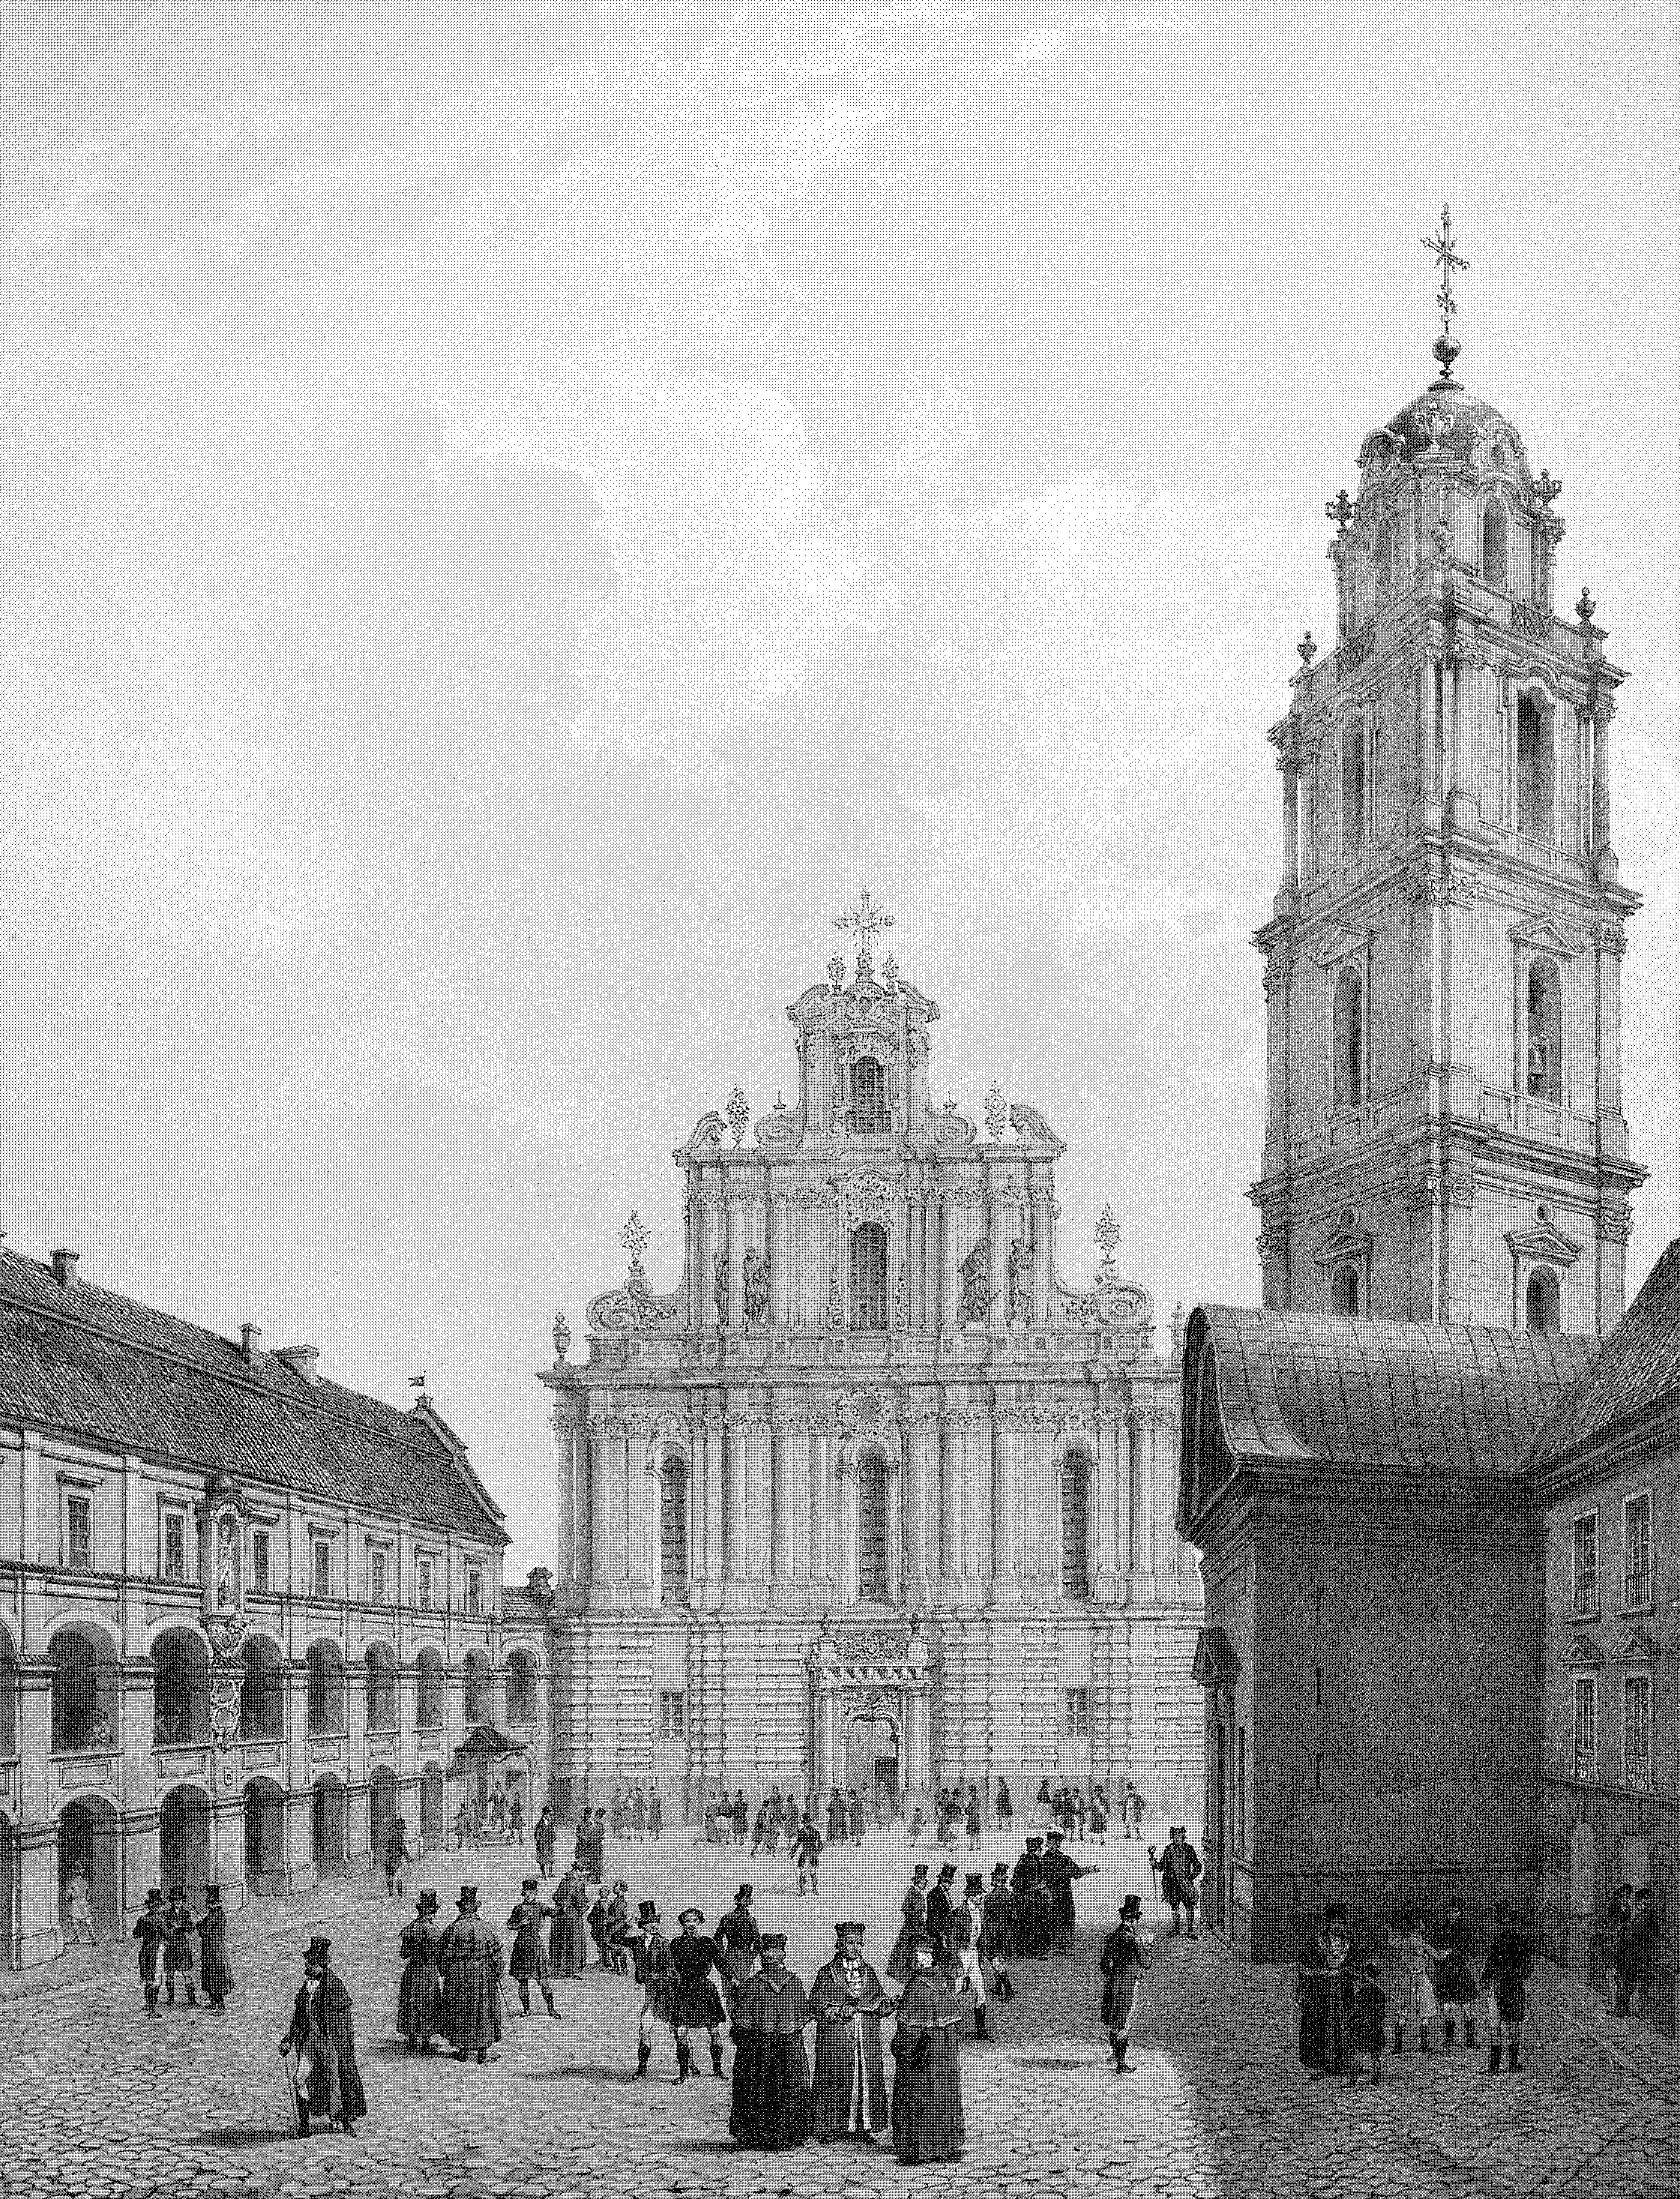
\includegraphics[width=\textwidth]{ilustra-05.png}
    \caption{Esplendor barroco da Universidade de Vilna, por volta de 1820.}
\end{figure}

Em 1610, o exército unido polono"-lituano ocupou Moscou e coroou o filho do rei
polonês como tzar. Com a ajuda dos jesuítas, São Casimiro se tornou
santo padroeiro da Lituânia, da Polônia e da Rússia. Dez anos depois,
como símbolo da vitória católica sobre a ortodoxia russa, seu dia de
festa, celebrado em 4 de março, dia de sua morte, foi estendido para
toda a igreja católica.

Embora a vitória polono"-lituana tenha durado pouco, o enorme botim
trazido de Moscou enriqueceu Vilna, favorecendo as ambições
arquitetônicas dos jesuítas. A consagração da colossal igreja de São
Casimiro em 1618, contudo, coincidiu com o início da Guerra dos Trinta
Anos, que deixou quase toda a Europa Central em ruínas. E, no momento em
que as relíquias de São Casimiro, guardadas num sarcófago de prata,
foram depositadas em 1636 na elegante capela barroca da catedral da
cidade, a Lituânia estava à beira da aniquilação. Na Polônia"-Lituânia, a
décadas de guerra se seguiu um desastroso período de discórdias internas
e externas, que ficou conhecido mais tarde como Dilúvio (1648--1667).
Forças moscovitas saquearam a Lituânia e, entre 1655 e 1661, ocuparam
Vilna, onde o tzar russo Alexei Mihailovich se auto"-declarou grão"-duque
da Lituânia. Enquanto o corpo de São Casimiro era salvo pelas forças
lituanas que batiam em retirada, o exército russo profanava as várias
igrejas católicas e greco"-católicas da cidade.

Apesar de tudo, em meio à ruína das guerras, o estilo barroco floresceu,
enriquecendo o sarmacismo com o teatralismo metafísico da época. Mais
especificamente, o apogeu alegórico do sarmacismo correspondeu à
libertação gloriosa de Viena do cerco turco por parte do exército
polono"-lituano, liderado pelo rei Jan Sobieski em 1683. Entretanto, para
a República, os despojos políticos da vitória duraram pouco. Um desfile
interminável de invasores estrangeiros, dos suecos aos cossacos
ucranianos, e dos otomanos aos moscovitas, marchou pelo país. As
fronteiras vulneráveis da República, porém, desempenharam um importante
papel na formação das peculiaridades da cultura sarmácia. E enquanto
diversas ``práticas locais proviessem da expressividade do barroco
pan"-europeu\ldots{} elas desenvolveram, na República Polono"-Lituana,
formas únicas em parte devido a seu extenso contato com as civilizações
russa e otomana.''\footnote{Daniel Stone, \textit{The Polish"-Lithuanian State, 1386--1795}. Seattle: University of Washington Press, 2001, pp. 211--213.}

Essa porosidade continental foi contrariada pelo isolacionismo local.
Diante da aniquilação política, o nativismo substituiu o cosmopolitismo
e, tendo ``perdido toda esperança de salvação, a sociedade polonesa se
voltou para si mesma e, enfeitiçada pelos ideais imaginários da `Velha
Sarmácia', começou a perder de vista as realidades
elementares.''\footnote{Davies, op. cit., p. 367.} Durante o assim
chamado Período Saxão (1697--1764), quando a República foi governada por
dois monarcas estrangeiros (os eleitores da Saxônia), o sarmacismo
adquiriu qualidades explícitas de introversão nostálgica e nativismo
sentimental. A \textit{szlachta}, ou nobreza polonesa, preencheu a Sarmácia
de memórias reais e ficcionalizadas do passado. Nesse sentido, a
Sarmácia era mais um palimpsesto do que um país, um reino imaginável e
legível --- um topos reconhecível --- formado por remendos de elementos
familiares de mitologia, genealogia, história e geografia. Era real por
ser decifrável. A realidade representacional da Sarmácia encontrava
apoio no teatralismo da imaginação barroca, que misturava livremente
épicas da Antiguidade, cenas bíblicas, locais exóticos, temas
fantásticos e eventos políticos da Europa contemporânea num drama que se
desdobrava no quotidiano.

Diversos rituais diários, cerimônias oficiais, gestos habituais,
diatribes oratórias e, claro, a língua, mantiveram a nação sarmácia da
nobreza polono"-lituana separada de outras nações circundantes. A
\textit{szlachta} polonesa vestia trajes especificamente sarmácios, seguia
práticas religiosas e sociais exclusivamente sarmácias, e sofria até
mesmo de uma estranha patologia médica, explicitamente identificada em
latim como \textit{plica polonica}, descrita uma vez por um médico suíço
do século \textsc{xviii} como ``um humor viscoso e acre penetrando pelos cabelos''
com os sintomas gerais de ``coceira, inchaço, erupções, úlceras, febre
intermitente, dor na cabeça, prostração, desânimo, reumatismo, gota e
por vezes até mesmo convulsões, paralisia e insânia.'' A doença, assim
como a filiação à nação da Sarmácia, era presumidamente hereditária,
mas, para o horror dos estrangeiros, também ``provou ser contagiosa
quando em estado virulento.''\footnote{Conforme citado em Larry Wolff, \textit{Inventing Eastern Europe: The Map of Civilization on the Mind of the Enlightenment}. Stanford: Stanford University Press, 1994, p. 30. Para maiores informações sobre o estilo sarmácio, ver Marija Matušakaitė, \textit{Apranga \versal{xvi}--\versal{xviii} a. Lietuvoje}. Vilna: Aidai, 2003, pp. 95--222; e também Gražina Marija Martinaitienė, ``At the crossings of western and eastern cultures: the contush sashes'' em \textit{Lietuvos Didžiosios Kunigaikštystės barokas: formos, įtakos kryptys}. Acta Academiae Artium Vilnensis 21 (2001), pp. 167--175.}
É difícil dizer como era a Vilna do período barroco sarmácio. A
composição das autoridades municipais revela um padrão de fragmentação
étnica, com poloneses compondo cerca de cinquenta por cento, trinta por
cento de rutenos, oito por cento de alemães, quatro por cento de
italianos e algumas pequenas minorias de origens lituana e húngara. A
população geral era ainda mais diversa, uma vez que os judeus, os
tártaros, os lituanos da classe baixa e os estrangeiros não podiam
participar do governo local. Membros de ordens religiosas ou de famílias
nobres também estavam excluídos da lista dos cidadãos urbanos. Mesmo
após a Contra"-Reforma liderada pelos jesuítas, a elite urbana permaneceu
dividida do ponto de vista religioso: os católicos dominavam a política
urbana, mas por pouco, pois constituíam cerca de sessenta por cento das
autoridades eleitas; em segundo lugar vinham os greco"-católicos --- cerca
de trinta por cento; e então protestantes e ortodoxos, cada um
compreendendo cerca de três por cento da elite. (Cabe recordar que,
depois de 1666, fiéis protestantes e ortodoxos foram proibidos de ocupar
cargos municipais, o que alterou sobremaneira o quadro demográfico da
classe governante da cidade.)\footnote{Aivas Ragauskas, \textit{Vilniaus miesto valdantysis elitas: \versal{xvii} a. antrojoje pusėje}. Vilna; Diemedžio leidykla, 2002, p. 448.}
Nos arredores imediatos da cidade, as diversificadas comunidades de
cristão, judeus, caraítas e muçulmanos viviam próximas umas das outras,
de modo que Vilna se transformou no ponto de encontro para todo um grupo
de idiomas: lituano, eslavo (polonês, ruteno, russo, antigo eslavônico
eclesiástico), latim, alemão, iídiche, hebraico e túrquico. Os
estrangeiros rapidamente encontravam seu equivalente bíblico naquela
infame Babilônia. Tal alusão trazia consigo um duplo significado, pois
implicava tanto num grande fascínio pela realidade local, como também
numa severa condenação da mesma. Aos olhos de vários estrangeiros e de
alguns habitantes locais, em especial os jesuítas, o multiculturalismo
da cidade era percebido mais como maldição do que como bênção.

O sarmacismo era privilégio social da nobreza, e a residência de campo
era seu principal domínio cultural. Vilna, apesar do estatuto político
diminuído, a riqueza reduzida, a população minguante e o crescente
provincialismo, ainda era, de longe, a maior cidade da região. Em 1645,
Vilna, sem considerar os subúrbios, contava cerca de 300 edifícios de
tijolo e 200 casas de madeira, e uma população de cerca de cinqüenta mil
pessoas.\footnote{Algimantas Miškinis e Vytautas Jurkštas, em \textit{Vilniaus architektūra}. Vilna: Mokslas, 1985, p. 9. Mais especificamente, os cidadãos possuíam 233 casas de tijolo e 163 casas de madeira, os nobres possuíam 53 e os judeus possuíam 49 casas (tijolo e madeira).} Entretanto, a nobreza local dominava a cidade, tanto cultural como politicamente. Em geral, a \textit{szlachta}, que
compunha cerca de dez por cento da população polono"-lituana, era um dos
grupos sociais mais privilegiados da Europa. Os nobres tinham o direito
de se reunir em assembleia para eleger o governante do país.
Determinavam também as questões relativas a impostos, política externa e
guerra, gozando inclusive do direito de se revoltar contra políticas
estatais impopulares. Com esse poder enorme nas mãos, a nobreza do país
tratava a cidade como seu próprio quintal. Na verdade, a nobreza local
possuía diversos edifícios na cidade e financiara a construção de belas
igrejas barrocas. A fachada sarmácia de Vilna era também matizada pela
determinação da camada superior da nobreza lituana em manter vivas as
associações alegóricas com Roma. Desde o Renascimento, as famílias mais
poderosas haviam identificado suas raízes genealógicas nas tribos
perdidas de antigos guerreiros romanos, visualizando a cidade como um
duplo sarmácio de Roma. Embora imperfeita, tal visão prolongou a
vitalidade artística do estilo barroco, que ali durou mais do que na
Europa Ocidental.

Paz e concórdia eram escassas na Vilna do século \textsc{xviii}, com ondas de
exércitos estrangeiros sempre trazendo destruição. Em 1702, o exército
sueco pilhou Vilna; em 1705, o exército russo, liderado por Pedro \textsc{i},
ocupou a cidade --- e foi logo seguido por forças saxãs. Em 1710, a peste
matou cerca de trinta e cinco mil habitantes (decerto mais da metade da
população) e, em 1720, uma rebelião violenta da classe baixa varreu a
cidade. Incêndios devastadores ocorriam regularmente: em 1715, 1737
(três quartos da cidade foram afetados por esse incêndio), 1741, 1748 e
1749. Do ponto de vista econômico e político, a cidade jamais conseguiu
se recuperar totalmente da sucessão de desastres sociais e naturais.
Apesar desses e outros acontecimentos catastróficos, ou talvez por causa
deles, esse período foi justamente o que marcou o esplendor barroco de
Vilna. Numa larga linha do tempo de evolução estética, o ano de 1750 é o
divisor de águas entre as sensibilidades barroca e neoclássica. Naquela
altura, o culto da racionalidade iluminista havia chegado a todas as
grandes capitais europeias, remodelando"-as: Paris, Londres, Viena,
Berlim, Nápoles e São Petersburgo. Na provinciana Vilna, contudo,
maneiras antiquadas ainda reinavam supremas e, na década de 1770, os
``arquitetos na Lituânia desenvolveram suas próprias formas originais,
que podem ser também vistas como extraordinária extensão das tradições
barrocas e rococó.''\footnote{Kaufmann, op. cit., p. 421.} Esse foi um
período em que amadureceu o assim chamado barroco de Vilna, e igrejas
ainda mais elaboradas foram encomendadas e construídas na cidade por
ricos magnatas lituanos, que alicerçavam suas fortunas em vastos
latifúndios. Como resultado da proliferação arquitetônica, no fim do
século \textsc{xviii}, numa cidade de menos de quarenta mil habitantes, havia trinta
e duas igrejas católicas com quinze mosteiros, cinco igrejas
greco"-católicas com três mosteiros, uma igreja ortodoxa russa, uma
luterana e uma calvinista.\footnote{\textsc{j}.\,Jurginis, \textsc{v}.\,Merkys e \textsc{a}.\,Tautavičius, \textit{Vilniaus miesto istorija: nuo seniausių laikų iki Spalio revoliucijos}. Vilna: Mintis, 1968, p. 190.}

O barroco de Vilna reverteu o relógio da evolução urbana europeia e, ao
invés de impulsionar a paisagem da cidade rumo ao sentido neoclássico de
ordem espacial, ele pareceu reordená"-la de volta para suas origens
medievais. Assim, não há em Vilna eixos retos, praças simétricas ou
vistas emolduradas de ruas --- características de cidades barrocas. Em
outras cidades, o espaço barroco se expande horizontalmente; em Vilna,
ele jorra verticalmente, como a fumaça de um fogo ritual que tenta
aplacar os céus ao invés de competir com eles. É claro que a
persistência local do barroco era também uma ilusão, pois Vilna, junto
com todo o resto da Polônia"-Lituânia, não estava imune às mudanças
intelectuais, estéticas e políticas do seu tempo. O esplêndido outono do
barroco de Vilna foi um gesto elegante e efêmero do desenvolvimento
estético atrasado da cidade, um gracioso adeus à sua fantástica era de
ouro.

A longevidade do barroco local não encantava os visitantes cujas ideias
sobre o mundo e a arte já estavam determinadas pelos métodos modernos da
observação científica e pelos valores iluministas do julgamento secular.
Quando o termo ``barroco'' foi introduzido pela primeira vez em meados
do século \textsc{xviii} na França, ele trazia consigo um significado extremamente
negativo, se não depreciativo. O \textit{Dictionare de l'Académie
française}, de 1740, definia barroco como algo ``irregular, estranho,
{[}e{]} desigual'' que implicava numa falta de separação entre as
esferas do real e do imaginário.\footnote{Rosario Villari, ``Introduction'' em \textit{Baroque Personae}. Chicago: University of Chicago Press, 1995, p. 2.} O pensamento racionalizado do período iluminista, por outro lado, ``possibilitava
separar aquilo que no barroco havia sido percebido como unidade: arte,
sociedade, moral, costumes, ou seja, a ideia barroca da conjunção entre
realidade e aparência. A mente iluminista penetrava nas aparências a fim
de revelar a ficção da sociedade barroca, exibindo assim as distinções
entre arte e luxo, gosto e moda, moral e estética, sujeito e
objeto.''\footnote{Remy \textsc{g}.\,Saisselin, \textit{The Enlightenment against Baroque: Economics and Aesthetics of the Eighteenth Century}. Berkeley: University of California Press, 1992, p. 6.} Enquanto a sociedade europeia fundada em ilusões teatrais e alusões metafísicas
dava lugar a uma sociedade construída sobre a ciência natural e o
escrutínio público, os alquímicos desejos sarmácios de transformar a
parca realidade numa rica fantasmagoria eram apreciados como
experimentos culturais e políticos de frivolidade e irresponsabilidade
social.

\chapter{As sombras do Iluminismo}

%\setlength{\epigraphwidth}{.45\textwidth}
\begin{epigraphs} 
\qitem{Onde hordas bárbaras da montanha cítia vagueiam,\\
Verdade, Misericórdia, Liberdade ainda encontrarão \qb{}seu lar\ldots{}\\
Oh, imagem ensanguentada no livro do Tempo,\\
A Sarmácia tombou, sem pranto, sem um só crime.}{``Polônia'', \textsc{thomas campbell}}
\end{epigraphs}

Quando o renomado viajante e naturalista Johann Georg Adam Forster se
estabeleceu na capital lituana em 1784, ele encontrou a cidade barroca
em declínio. ``Cem anos atrás,'' escreveu Forster a seu melhor amigo na
Alemanha, ``\textit{Wilna} tinha 80 mil habitantes. Hoje, se incluirmos seus 12
mil judeus --- ela tem apenas 20 mil.''\footnote{Georg Foster escreve para Samuel Thomas Sömmerring, 12--13 de dezembro de 1784, \textit{Georg Forsters Werke: Sämtliche Schriften, Tagebücher, Briefe (Briefe 1784 -- Juni 1787)}, vol. 14. Berlim: Akademie Verlag, 1978, p. 232. O fisiólogo e anatomista alemão Sömmerring (1755--1830) foi um dos amigos íntimos de Forster.} A observação estatística de Forster era mais do que o comentário casual de um cientista
desapaixonado. Era um lamento, uma avaliação angustiada da condição
humana. \textit{Wilna}, considerava Forster, era uma antítese do progresso
humano, um remanso provinciano nem mesmo digno do título de cidade,
muito menos de capital de um país europeu. Para Forster, \textit{Wilna} era no
máximo um lugar de exílio --- um purgatório da era científica do
Iluminismo --- em que almas europeias desprovidas de sorte e de intelecto
são mantidas na idade das trevas das superstições e do barbarismo. A
cidade não mais denotava a periferia inculta da Europa; ela era agora
uma fronteira bravia onde a civilização urbana retornava para o seu
estado selvagem.

A antipatia de Forster pela capital da Lituânia (país ainda grande,
embora castigado pela pobreza) se deveu ao prisma de sua educação
cosmopolita, vivência transformadora, incomum mesmo para sua idade, de
internacionalismo acadêmico e vasta experiência de viagem pela Europa.
Forster jamais participou de um \textit{grand tour} da Europa, evento
social que se tornara extremamente popular entre os jovens aristocratas
e intelectuais do século \textsc{xviii}; por outro lado, realizara a circunavegação
da Terra. Uma viagem ao redor do mundo levou Forster a \textit{Wilna}. Em 1772,
aos dezessete anos de idade, participou, junto com o pai, cientista
também ele, da segunda expedição do Capitão Cook ao Pacífico Sul, a
bordo do \textit{\textsc{h.\,m.\,s.} Resolution}. Num tempo em que a Europa mal podia
imaginar o lado mais distante do mundo, o jovem Forster pesquisou e
documentou os habitantes do Taiti, da Nova Zelândia e das desoladas
ilhas da Terra do Fogo, confraternizando com eles. Em seguida, Forster
publicou um livro, \textit{Uma viagem ao redor do mundo}, detalhando
descobertas científicas e impressões pessoais da viagem. O manuscrito em
dois volumes e 1200 páginas, concebido, nas palavras do jovem autor,
como ``uma história filosófica da viagem'', foi publicado em inglês e
alemão.\footnote{George Forster, \textit{A Voyage Round the World}, vol. 1. Honolulu: University of Hawai'I Press, 2000, p. 6.}
Forster era um cientista com alma de artista revolucionário, que,
segundo seus contemporâneos, ``demonstrava sua receptividade e educação
universal combinando a elegância francesa com formas populares de
apresentação, e a utilidade inglesa com a profundidade alemã de
percepção e espírito.''\footnote{Friedrich Schlegel, \textit{Kritische Schriften}, conforme citado no livro de Thomas \textsc{f}.\,Saine, \textit{Georg Forster}. Nova York: Twayne Publishers, 1972, p. 13.} O livro, habilmente ilustrado --- uma das responsabilidades de Forster durante a expedição era
a de desenhar as diversas descobertas --- transformou"-se em tema de
conversa nos salões iluministas da Europa. E enquanto acadêmicos mais
vigorosos levantavam objeções à subjetividade do autor, o tom do livro
se integrava perfeitamente ao espírito do Romantismo, que brotava em sua
busca de unidade entre racionalismo e imaginação. Algumas décadas mais
tarde, Alexander von Humboldt, geógrafo de primeira linha e esteta da
era moderna, agradeceu Forster por introduzir na ciência a ``força
descritiva do observador, o avivamento do elemento descritivo da
natureza, e a multiplicidade de visões.''\footnote{Alexander von Humboldt, \textit{Kosmos}, conforme citado em Forster, \textit{A Voyage Round the World}, vol. 1, op. cit., xl.}
O livro lançou a carreira profissional de Forster como cientista
``inato'', levando"-o a ser indicado como docente no Collegium Carolinum
na cidade de Kassel, no Hesse. O ambicioso naturalista ficou
profundamente insatisfeito com o diminuto encargo, ele que nutria a
esperança de alcançar o mesmo estatuto acadêmico do pai, que havia se
tornado professor na prestigiosa Universidade de Halle, sob o patrocínio
de um monarca iluminista, Frederico, o Grande, da Prússia. No outono de
1783, Forster recebeu um convite da Universidade de Vilna e, diante da
falta de perspectivas na Alemanha, decidiu se mudar para a Lituânia.

\textit{Wilna} se localiza a cerca de 1100 quilômetros a nordeste de Kassel. No
fim do século \textsc{xviii}, em boas condições meteorológicas, essa distância podia
ser facilmente coberta numa questão de poucas semanas. A viagem de
Forster a \textit{Wilna} durou quase seis meses. Ele quis conhecer mais das
terras alemãs a fim de aprofundar seus contatos profissionais e adquirir
conhecimentos acadêmico de valia. Durante a viagem, Forster explorou de
bom grado os prazeres sociais de sua fama literária. Na cidade mineira
de Freiberg, na Saxônia, o naturalista se encontrou com o príncipe
Stanislaw Poniatowski (filho), sobrinho do rei da Polônia e tesoureiro
do Grão"-Ducado, quem, nas palavras de Forster, ``retratou os lituanos da
maneira mais positiva.''\footnote{Forster escreve para Sömmerring, 2 de julho de 1784, \textit{Georg Forsters Werke 14}, op. cit., p. 114.} Embora o jovem Poniatowski reconhecesse os problemas sociais e
econômicos do país como resultantes de ``cabeças demais com opiniões
demais'', ele fez também observações alentadoras sobre a expansão ``do
Iluminismo\footnote{No original, \textit{Aufklärung}.} na Polônia.'' O príncipe preveniu
Forster sobre a lenta penetração das ideias progressistas na Lituânia,
porém descreveu \textit{Wilna} como ``o lugar mais agradável da Polônia, com uma
universidade de melhor reputação do que a Universidade de
Cracóvia.''\footnote{Ibid., pp. 113--114.}

%{[}figura 21{]}
%
%``Mapa de Willda ou Willna na Lituânia'', 1737.

Após o breve desvio pela Saxônia, Forster chegou a Viena, onde se
demorou por alguns meses gozando de banquetes, reuniões de salão e
saraus aristocráticos. A sociedade vienense saboreava as histórias
picantes de Forster sobre os hábitos e costumes (inclusive os sexuais)
das sociedades das ilhas do Pacífico. Forster, por sua vez, considerava
Viena um paraíso, amargurando"-se com a ideia de uma inevitável partida.
Quando o dia chegou, escreve Forster, ``todos os meus amigos e o
{[}príncipe{]} Kaunitz me insuflaram a esperança de poder retornar
depois de deixar a Polônia. Até o imperador me disse: `Acho que vou
vê"-lo em breve de novo em Viena, pois você não será capaz de suportar
ficar com os poloneses por muito tempo.'"\footnote{Forster, conforme citado em Saine, op. cit., p. 163.} O imperador demonstrou também certo ceticismo quanto à perspectiva de difusão do Iluminismo na
Lituânia: ele não acreditava haver uma universidade em \textit{Wilna}, nem a
perspectiva de ensinar ciências naturais a seus habitantes parecia lhe
fazer qualquer sentido. Antes de aprenderem qualquer coisa sobre
ciência, os poloneses, observou o imperador, precisam aprender o
alfabeto.

\asterisc

%{[}figura 22{]}
%
%O grande pátio da universidade em \textit{Wilna}, 1786.

No fim do século \textsc{xviii}, a Universidade de Vilna estava em transição. A
antiga Academia Jesuíta, criada em 1579 no intuito de apoiar a
Contra"-Reforma católica, constituía a fundação material e também, sob
muitos pontos"-de"-vista, intelectual da universidade. Após a dissolução,
a mando do papa, da Ordem dos Jesuítas em 1773, a academia passou a ser
administrada diretamente pelo estado lituano. Em 1781, ela se tornou a
escola suprema do Grão"-Ducado da Lituânia, supervisionada pela
recém"-criada Comissão de Ensino, que tentou criar o primeiro sistema
pedagógico integrado na Europa. Apesar do pensamento progressista,
recursos financeiros e vontade política para a implementação do projeto
eram limitados. A maior parte dos membros da universidade consistia em
seus antigos professores: ex"-padres e monges jesuítas secularizados;
ademais, o novo currículo pouco diferia do programa dogmático da velha
escola. A Comissão de Ensino, liderada pelo bispo de Płock, irmão do rei
da Polônia, procurou ativamente seduzir várias celebridades acadêmicas
europeias até \textit{Wilna}. A cadeira de ciências naturais da universidade foi
a princípio oferecida ao pai de Forster, que detinha uma reputação
acadêmica muito mais vasta. Quando Forster pai recusou a oferta, ele
habilmente propôs o filho. A Comissão concordou em empregar o jovem
Forster, estipulando que recebesse o título de doutor dentro de um ano
após chegar a \textit{Wilna}. Além de extenuantes responsabilidades docentes, ele
deveria também instituir um jardim botânico com flora lituana, criar um
programa agronômico e proceder à pesquisa sobre o eventual potencial
mineiro e industrial a partir de recursos naturais locais. O jovem
Forster, desgraçadamente, não tinha o treinamento necessário para
atender tais expectativas. Embora fosse doutor pela Universidade de
Halle, ele conhecia muito pouco do mundo natural da Lituânia, práticas
agrícolas contemporâneas ou métodos industriais de desenvolvimento
econômico.

Forster via em seu posto em \textit{Wilna} uma jogada profissional para resolver
problemas pessoais. Estava descontente com sua vida de solteiro em
Kassel, onde frivolamente havia se ligado à Franco"-maçonaria, caíra na
farra e se endividara bastante. A fim de tornar mais confortável e
produtiva sua existência na remota \textit{Wilna}, ele procurou uma esposa. Logo
antes de partir rumo à Lituânia, Forster pediu a mão de Therese Heyne,
filha do amigo e colega Christian Gottlob Heyne, professor de filologia
clássica na Universidade de Göttingen. Há pouca evidência de faíscas de
amor entre os noivos. Forster não era um homem muito vistoso e, para sua
idade, tinha uma saúde que deixava a desejar. Os três anos passados no
mar fizeram"-no perder quase todos os dentes devido ao escorbuto;
ademais, passou a sofrer de diversos problemas digestivos, infecções
recorrentes e reumatismo. Therese, dez anos mais jovem, bela e
excepcionalmente bem educada, teve por bem responder à gentileza,
reputação intelectual e potenciais perspectivas acadêmicas de Forster.
Uma vez acertado, o casamento foi adiado por um ano, até que Forster se
estabelecesse solidamente em \textit{Wilna}. Nesse ínterim, os dois se tornaram
íntimos correspondentes, trocando longas e detalhadas missivas (não de
amor, infelizmente) toda semana.

As primeiras impressões de Forster sobre o lugar foram capturadas em sua
correspondência confidencial com Therese, seus amigos mais próximos e
familiares. A República não era estranha a Forster, que nascera em 1754
no vilarejo de Nassenhuben, na região do delta do Vístula, onde os
idiomas polonês e alemão se entrelaçavam livremente. O cientista cresceu
num lar protestante de fala alemã, embora a família Forster tivesse
ancestrais que tinham chegado à Polônia na década de 1640, vindos da
Escócia e Inglaterra. Mas visto que a região de seu local de nascimento
permanecera em possessão polonesa até 1793, Forster, nominalmente, era
um súdito polonês. Sua reação, porém, à Polônia"-Lituânia era em geral a
de um perfeito estrangeiro. Via de regra, a atitude alemã com relação à
Polônia"-Lituânia era condescendente. O país era considerado um
anacronismo político sem qualquer valor para a cultura do Iluminismo.
Goethe, que realizou uma viagem de uma semana de Weimar até Cracóvia em
1790, laconicamente recapitulou essa visão alemã da Polônia: ``Nesses
oito dias vi muitas coisas notáveis, mesmo que em sua maioria tenham
sido apenas notavelmente negativas.''\footnote{Goethe, conforme citado em Wolff, op. cit., p. 333.}
Outros europeus deixaram impressões mais dramáticas sobre o país.
Forster viajou para \textit{Wilna} por uma estrada importante, via Varsóvia,
Białystok e Grodno, no meio do outono. Um ou dois meses mais tarde,
precisamente a mesma rota foi percorrida pelo conde Louis"-Phillipe de
Segur, enviado \textit{extraordinaire} de Luís \versal{xvi} à corte imperial russa
em São Petersburgo. Segur descreveu uma desagradável sensação de
deslocamento ao passar a fronteira da Prússia com a Polônia:

\begin{quote}
Atravessando a parte oriental das propriedades do rei da Prússia,
poder"-se"-ia dizer que se abandona um teatro em que reinam a natureza
adornada pelos esforços da arte e a perfeita civilização. Os olhos já se
entristecem com a poeira áspera, com a floresta vasta. Mas tão logo
adentramos na Polônia, tem"-se a impressão de deixar a Europa
completamente para trás, e um novo espetáculo impressiona a vista: um
imenso país quase todo coberto por abetos sempre verdes, mas sempre
tristes, interrompidos a longos intervalos por uma ou outra planície
cultivada, como ilhas espalhadas no oceano; habitantes pobres,
escravizados, vilarejos imundos; casebres pouco diferentes de cabanas
selvagens; tudo leva a crer termos voltado dez séculos, e estarmos em
meio a hordas de hunos, cítios, vênetos, eslavos e sarmácios.\footnote{Louis"-Phillipe de Ségur, \textit{Mémoires, souvenirs, et anecdotes, par le comte de Ségur}, vol. 1, conforme citado em Wolff, op. cit., p. 19.} \end{quote}

Segur tinha a mesma idade de Forster e, assim como ele, era também um
viajante experimentado (havia passado algum tempo na América do Norte).
Mas o conde era o rebento de uma das famílias mais ricas da França e, à
diferença do cientista, gozara até então de todos os confortos à
disposição para viajar. Atravessando a República de trenó durante o
inverno, malgrado a melancólica introdução, ele vivenciou a viagem como
uma experiência jovial através de ``um inconcebível amálgama de séculos
antigos e séculos modernos, de espírito monárquico e espírito
republicano, de orgulho feudal e igualdade, de pobreza e
riquezas.''\footnote{Ibid., pp. 19--20.} No entanto, a desventura o
alcançou em algum ponto entre Białystok e Riga, onde, por causa de uma
terrível tempestade de neve, ele foi forçado a deixar sua bagagem para
trás. O diplomata jamais haveria de recuperar seus pertences e, meses
mais tarde, em resposta a indagações oficiais, ele recebeu um estranho
relatório das autoridades locais, afirmando que tudo o que lhe pertencia
fora perdido num incêndio no meio da gélida Lituânia.

William Coxe (1747--1828), inglês experiente, em 1778 atravessou a
Lituânia rumo à Rússia durante um \textit{grand tour} da Europa, como
tutor e companheiro de viagem de um jovem aristocrata inglês. Coxe faz
menção à monotonia e à paisagem inalterável durante o trajeto,
semelhante a uma enfadonha travessia do mar: ``Jamais vi uma estrada tão
estéril de paisagens interessantes como aquela entre Cracóvia e
Varsóvia. Não há absolutamente nada, durante o trajeto inteiro, que seja
capaz de chamar a atenção, por um momento que seja, do mais curioso
viajante.''\footnote{William Coxe, \textit{Travels in Poland, Russia, Sweden and Denmark}. Londres: \textsc{j}.\,Nicholas, 1784, p. 148.} Se atravessar a Polônia, porém, era uma atividade insípida, caminhar pela Lituânia era
uma demorada aventura com final pitoresco: ``As estradas deste país,''
observa Coxe, ``estão descuidadas, muito poucas delas sendo superiores a
caminhos vicinais serpenteando pela floresta espessa sem o mínimo grau
de orientação artificial: elas são com frequência tão estreitas que mal
permitem a passagem de uma carruagem; são continuamente obstruídas por
troncos e raízes de árvores e, em alguns trechos, tão arenosas que oito
cavalos pequenos mal conseguem nos puxar.''\footnote{Ibid., p. 226.} Ao
penetrar nos bosques, diante dos olhos do viajante cansado se desabria
uma paisagem cada vez mais bizarra: ``as cidades e os vilarejos eram
compridos e espalhados; todas as casas, inclusive as igrejas, são de
madeira; multidões de mendigos rodeavam nossa carruagem sempre que
parávamos; os judeus se faziam presentes sem cessar.''\footnote{Ibid., p. 211.}
%{[}figura 23{]}
%
%Comerciantes judeus perto de \textit{Wilna}.

Na Lituânia, à diferença da maior parte da Europa e da Rússia, a
comunicação quotidiana dos viajantes com o universo local que
atravessavam era mediada pelos judeus, que administravam quase todas as
necessidades mercantis e de viagem do país. ``Se você pedir um
intérprete, eles trarão um judeu; se você chegar a uma estalagem, o dono
é judeu, se você precisar de um correio a cavalo, quem providencia é um
judeu e o mensageiro é um judeu; se você quiser fazer compras, o seu
agente é um judeu: e este é o único país da Europa em que os judeus
cultivam a terra: ao atravessar a Lituânia, não raro os vimos semeando,
colhendo, ceifando e realizando outros trabalhos agrícolas.''\footnote{Ibid., p. 226.} Os judeus não eram essenciais apenas para tornar a viagem mais confortável, mas sua ``aparência pouco familiar'' animava a mente
fatigada do viajante:

\begin{quote}
Vimo"-nos no meio de um imenso celeiro ou galpão, no fundo do qual
vislumbramos dois grandes pinheiros em chamas, com galhos e tudo, numa
lareira sem chaminé: ao seu redor, diversas pessoas, completamente
vestidas de preto e ostentando longas barbas, estavam ocupadas em
mexer um enorme caldeirão suspenso sobre o fogaréu. Se acreditássemos em
feitiçaria, ou em um pouco de superstição, facilmente teríamos tomado
aquele grupo por bruxos encarregados de algum ritual místico;
entretanto, após um exame mais minucioso, acabamos por neles reconhecer
nossos velhos amigos judeus, que preparavam o seu e o nosso
jantar.\footnote{Ibid., pp. 230--31.}
\end{quote}

Aliás, Coxe foi um dos poucos estrangeiros que tentaram identificar a
patogênese da \textit{plica polonica}, apontando três causas principais da
doença, a saber, a instável e insalubre ``natureza do ar polonês, a
deletéria água local e a flagrante desatenção à limpeza por parte dos
habitantes.''\footnote{Ibid., p. 234.}

Esse mesmo retrato deprimente e fantasmagórico da Lituânia foi
contestado por outros viajantes, que o consideraram um exagero
fantasioso da realidade. Numa resposta direta ao relato de Coxe,
Friedrich Schulz, escritor alemão obscuro, deixou uma descrição que
procura corrigir a anterior. ``Quem viaja rumo à Rússia, quem lembra ou
quem descobre a maçante monotonia das estradas de e para Berlim\ldots{}
vai me agradecer por isso. A estrada {[}que atravessa a Lituânia{]} não
é muito mais longa que a estrada que vai até Berlim, embora viajar aqui
seja muito mais barato e mais rápido, por uma paisagem rural mais
agradável, generosa e populada por gente cortês. Não acredite nos boatos
de perigos. Já percorri essa estrada três vezes, assim como vários de
meus conhecidos, e nenhum de nós jamais viu nada suspeito de dia nem de
noite.''\footnote{Friedrich Schulz em Jurginis e Šidlauskas, op. cit., p. 106.} O relato de Schulz não continha apenas fatos objetivos; ele, também, se baseou no próprio conhecimento artístico para capturar as
sensações e as cores do quotidiano. Certa vez, ficou numa hospedaria de
donos judeus até altas horas da madrugada na ``improvável companhia de
soldados russos, lituanos seminus, poloneses embriagados e uma enorme
família de israelitas. Várias figuras dessa estalagem poderiam constar
nas pinturas de Fielding ou Hogarth. Mas eles de tal maneira me
impressionaram, que jamais procurarei de novo por convívio
semelhante.''\footnote{Ibid., p. 97.}

Forster era um viajante mais melancólico. No início, deixou"-se
profundamente ofender pela pobreza e repressão em que viviam os
habitantes locais, e respondeu à sua miséria com humildade. ``Foi a
dilapidação, a imundície do ponto de vista moral e físico, a
semi"-selvageria e a semi"-civilização\footnote{No original, respectivamente \textit{Halbwildheit} e \textit{Halbkultur}.} das pessoas, a visão da terra arenosa por toda
parte coberta por bosques escuros, que ultrapassaram qualquer conceito
que eu pudesse ter. Chorei sozinho durante uma hora por toda aquela
gente atirada ao abismo --- e depois voltei aos poucos a mim
mesmo.''\footnote{Georg Forster escreve para Friedrich Heinrich Jacobi, 17 de dezembro de 1784, \textit{Georg Forsters Werke 14}, op. cit., pp. 248--249.} Mais tarde, as emoções haviam se modificado. ``Esse foi mais um momento de bobagem da minha parte,'' observou Forster para o amigo
Friedrich Heinrich Jacobi, filósofo sensualista alemão, ``mas agora que
me recobrei por completo posso reconhecer o ridículo do meu
comportamento.''\footnote{Ibid., p. 249.}

A cada dia de sua viagem, Forster se torna cada vez mais habituado à
Lituânia. Envia a Therese um relatório sociológico desde Grodno, onde,
durante a reunião do Sejm (parlamento), ``toda a nobreza polonesa e
lituana'' se reúne. ``Estou aos poucos começando a me habituar aos
costumes desta nação tão original\ldots{} já superei o choque inicial e
posso agora observar as coisas sem qualquer amargor\ldots{} {[}e{]}
apesar de algumas deficiências na Constituição liberal deste reino, é um
grande prazer notar que todo nobre polonês goza aqui de
liberdade.''\footnote{Georg Forster escreve para Therese Heyne, 12 de novembro de 1784, \textit{Georg Forsters Werke 14}, op. cit., p. 205.} Os habitantes locais, descreve Forster a seus outros destinatários,
adoram tudo o que seja francês e detestam tudo o que seja alemão. Isso
acaba gerando, segundo Forster, um efeito cultural negativo: ``Na
Polônia, chamar alguém de alemão --- é o pior dos insultos; como
resultado, a educação da alta nobreza foi totalmente entregue às mãos
dos barbeiros e \textit{modistes} franceses.''\footnote{Georg Forster escreve para Joachim Heinrich Campe, 9 de julho de 1786, ibid., p. 503.} E visto que ``a aristocracia polonesa segue o espírito francês, eles olham para tudo daquela maneira superficial e
enciclopédica.''\footnote{Forster escreve para Jacobi, 17 de dezembro de 1784, ibid., p. 249.}

Passados alguns dias, na estrada rumo a \textit{Wilna}, Forster participou de um
encontro singular. Numa das modestas estalagens, ele se juntou a um
divertido padre católico que bebia vodca com um velho mensageiro judeu.
Os camaradas divertiram o cientista com sua conversa estridente, em que
toda forma de autoridade era rejeitada. Os dois caluniavam todo o mundo:
desde o imperador do Sacro Império Romano Germânico e o rei polonês, até
o bispo de \textit{Wilna} e o abade local. Um ou dois dias depois, ainda de
ressaca, Forster chegou ao destino final, concluindo seu relato de
viagem sobre a Lituânia diante dos portões de \textit{Wilna}:

\begin{flushright}
\smallskip\hfill\textsc{18 de novembro de 1784}
\textit{Quinta"-feira, 5 horas da manhã}
\end{flushright}
\smallskip

\begin{quote}
Parto de uma
estalagem judaica paupérrima e chego às 9 da manhã a Gostki
ou Swetnik, a 4 milhas, numa outra estação de correio administrada por judeus, onde
troco de roupa e continuo o trajeto rumo a \textit{Wilna}, em 3 milhas, aonde chego
à uma hora da tarde. Uma milha antes de \textit{Wilna}, a paisagem ao longo do
rio Wilia se revela muito bonita: íngremes colinas de areia e penhascos
calcarosos coroados por uma esplêndida floresta verdejante. A
localização de \textit{Wilna} é surpreendentemente fabulosa; tão logo nos
aproximamos da cidade, a visão das colinas em derredor que descem até o
vale, onde toda essa grandiosa cidade, agraciada com tantas torres, se
localiza, é realmente impecável e magnífica. No interior da cidade ---
ruas estreitas e imundas e inúmeras ruínas --- entretanto, entre elas, é
possível encontrar um ou dois edifícios impressionantes. \textit{Finis
viaeque chartaeque}.\footnote{Georg Forster, \textit{Georg Forster Werke: Sämtliche Schriften, Tagebücher, Briefe}, vol. 12. Berlim: Akademie Verlag, 1978, p. 189.} 
\end{quote}

O naturalista transformou sua observação última --- fim da estrada e da
estória (frase satírica de Horácio, em que está implícita uma falta de
interesse em narrar) --- numa premonição. Ele imediatamente mandou um
aviso à sua noiva, concernente a suas perspectivas futuras na cidade.
Tinha pouco entusiasmo a transmitir:

%{[}figura 24{]}
%
%\textit{Wilna}: a muralha da cidade, 1785.

\begin{quote}
Em \textit{Wilna}, podemos ver como uma cidade outrora populosa entra em rápido
declínio: edifícios abandonados e montes de entulho estão por toda
parte. Aqui é possível encontrar gente desmoralizada, que se tornou
simplesmente indiferente a sua trágica condição; e, finalmente, podem"-se
testemunhar os resultados catastróficos do enxerto de uma nação
semi"-civilizada com vícios semi"-selvagens.''\footnote{Forster escreve para \textsc{t}.\,Heyne, 13 de dezembro de 1784, \textit{Georg Forsters Werke 14}, op. cit., p. 242.} Ele escasseou nos detalhes, observando que ``seria preciso um volume inteiro para descrever aquilo que, nas zonas
limítrofes alemãs, é tão engenhosamente chamado de \textit{polnische Wirtschaft} {[}economia polonesa{]}.\footnote{Forster escreve para \textsc{t}.\,Heyne, 24 de janeiro de 1785, ibid., p. 267.}
\end{quote}

\asterisc

Malgrado as origens alemãs, o jovem professor foi bem recebido pela
elite social da cidade. Gozou da hospitalidade local, embora nela
identificasse sinais de regressão cultural. ``A generosidade das
pessoas, aqui, como em todos os países sem cultura do mundo, é
impressionante; as pessoas socializam sem qualquer \textit{gêne}\footnote{Em português, ``embaraço''.} 
e até mesmo sua aparência é menos ordenada que em outros
lugares. A tolerância impera absoluta!''\footnote{Ibid., p. 269.} Logo o
pudico acadêmico se alarmou. ``Os poloneses se comportam de tal maneira
que não me deixam duvidar de minha presença sensual entre eles; ah, sim,
realmente experimento meu estar físico neste mundo lamentável, rodeado
por gente cruel, semi"-civilizada e semi"-selvagem deste país de florestas
desgrenhadas e tristes. [\ldots{}] Num tal país, sou obrigado a dizer adeus
a minhas ilusões\ldots{}''\footnote{Georg Forster escreve para Maria Wilhelmina von Thun, 24 de novembro de 1784, ibid., pp. 215--216.} Mais do que qualquer outra coisa, ele se irritou com a intimidade social (e
sexual) da elite de Vilna. Uma sensualidade cheia de flertes enlouqueceu
Forster, que se sentia impotente e perplexo diante dos costumes locais.
``Não há lugar em que as pessoas sejam mais sensuais que aqui. Ninguém
se interessa por outra coisa a não ser a descoberta de prazeres físicos.
O único prazer que posso ter aqui é corpóreo: se desejo socializar com
mulheres, preciso flertar sem parar; por vezes preciso até mesmo
acariciá"-las, pois todas elas querem ser estimuladas apenas de maneira
carnal. A sociedade sanciona completamente esse tipo de comportamento.
Aqui, é possível beijar em público o peito de uma donzela sem causar
escândalo!''\footnote{Forster escreve para Sömmerring, 3 de fevereiro de 1785, ibid., p. 271.} Forster se recusou a se acostumar aos hábitos locais e, logo após sua chegada, começou a ter fantasias de fuga.
``\textit{Wilna},'' declarou o desesperado naturalista a seu melhor amigo na
Alemanha, ``decerto não é um lugar em que possa permanecer para
sempre!''\footnote{Ibid., p. 273.} Num gesto impulsivo, ele decidiu
abandonar o cargo na universidade e fugir disfarçado para a mais exótica
e mais quente Constantinopla. A saúde debilitada e falta de dinheiro,
mais do que compromissos acadêmicos e a lógica profissional, curaram os
impulsos nômades de Forster.

Na verdade, \textit{Wilna} não era um lugar tão terrível, especialmente após a
chegada de Therese. Embora ``a cidade esteja num estado terrivelmente
deplorável,'' observou Forster, ``\textit{meo judicio}, ela ainda parece
muito melhor que Cracóvia e ultrapassa Grodno sobremaneira.''\footnote{Forster escreve para Sömmerring, 12 de dezembro de 1784, ibid., p. 232.} E, depois de passar as férias de verão na Alemanha, o professor confessou
que \textit{Wilna} era uma cidade muito mais grandiosa do que a maior parte das
cidades provinciais alemãs. Ele encarou o isolamento intelectual da
cidade como um desafio profissional. ``No final das contas'', escreveu
Forster a seu sogro em Göttingen, ``\textit{Wilna} é provavelmente o melhor lugar
do mundo para se ficar em paz, onde posso me dedicar meticulosa e
pacientemente ao estudo de temas interessantes; esse fato, por outro
lado, alivia minha terrível condição.''\footnote{Georg Forster escreve para Christian Gottlob Heyne, 10 de agosto de 1786, ibid., p. 521.} Numa carta enviada a Johann Gottfried Herder em Weimar, ele resumiu seu
papel em \textit{Wilna} como o de um missionário solitário do Iluminismo:
``Outrossim, o que consegui fazer aqui foi muito mais do que poderia ter
feito em qualquer outro lugar do mundo; vejo"-me como se estivesse
plantando uma semente de esperança.''\footnote{Georg Forster escreve para Johann Gottfried Herder, 21 de julho de 1786, ibid., p. 513.}

Não houve, contudo, nada a colher a partir das sementes de esperança de
Forster. Isso aconteceu, em parte, devido ao fato de Forster considerar
\textit{Wilna}, apesar de suas melhores intenções, indigna de seu talento:

\begin{quote}
Aqui, onde a ciência é coberta pelo silêncio da noite, onde conquistas
científicas não são recompensadas, nem mesmo com um simples prêmio
honorário, onde a maior parte das pessoas reconhecidas e celebradas são
só aquelas que possuem o maior número de servos ou que gastam as maiores
somas em jogos de azar --- aqui, um estrangeiro, devido à apatia de seus
compatriotas, aos poucos começa a se sentir abandonado pelo que há de
melhor na sociedade civilizada. [\ldots{}] A sociedade local é marcada
pela letargia, por adiamentos constantes e pela indiferença a tudo que
seja virtuoso; aqui, um viajante encontra tolerância e dissimulação de
delitos elementares, a persistência do habitual absurdo moralizador, a
falta de formas modernas de educação e, por vezes, um desprezo
implacável pelo estudo; ademais, o país é marcado por um patriotismo
insensato, uma estrutura governamental irracional e uma constituição
estatal doentia. Aqui, a opulência francesa se amalgama à bestialidade
sarmácia e, a fim de sobreviver e permanecer vigoroso e alerta do
ponto de vista mental, faz"-se necessário tornar"-se estático, inabalável
e fechar os olhos a todo esse absurdo. [\ldots{}] Em \textit{Wilna}, não há uma única
livraria e, em Varsóvia, existem apenas dois livreiros falidos, que só
comercializam romances indecentes.\footnote{Forster escreve para Campe, 9 de julho de 1786, ibid., pp. 502--503.} 
\end{quote}

Após a morte de Forster, Therese exprimiu uma visão mais equilibrada da
situação:

\begin{quote}
Eles não mantiveram sua palavra {[}em \textit{Wilna}{]} mas agora, depois de mais
de quarenta anos passados, acredito que, num certo sentido, Forster,
também, não manteve sua palavra, e surpreende"-me o fato de que Heyne
{[}o pai dela{]}, naquela altura, não lhe dera conselhos que eu não
poderia ter dado por falta de experiência e de entendimento. Forster
esperou que as promessas que lhe foram feitas fossem cumpridas para só
então poder realizar algo grandioso, ao passo que ele poderia ter
incrementado substancialmente sua posição caso houvesse realizado o
pouco que era possível com os meios diminutos à sua disposição, ao mesmo
tempo insistindo pelo cumprimento das promessas feitas.\footnote{Therese Forster, \textit{Johann Georg Forster's Briefwechsel}, conforme citado em Saine, op. cit., p. 43.} 
\end{quote}

%The retreat of the Grand Armeé through Vilna in 1812 (after the painting by J. Damel).
\begin{figure}[!h]
    \centering
    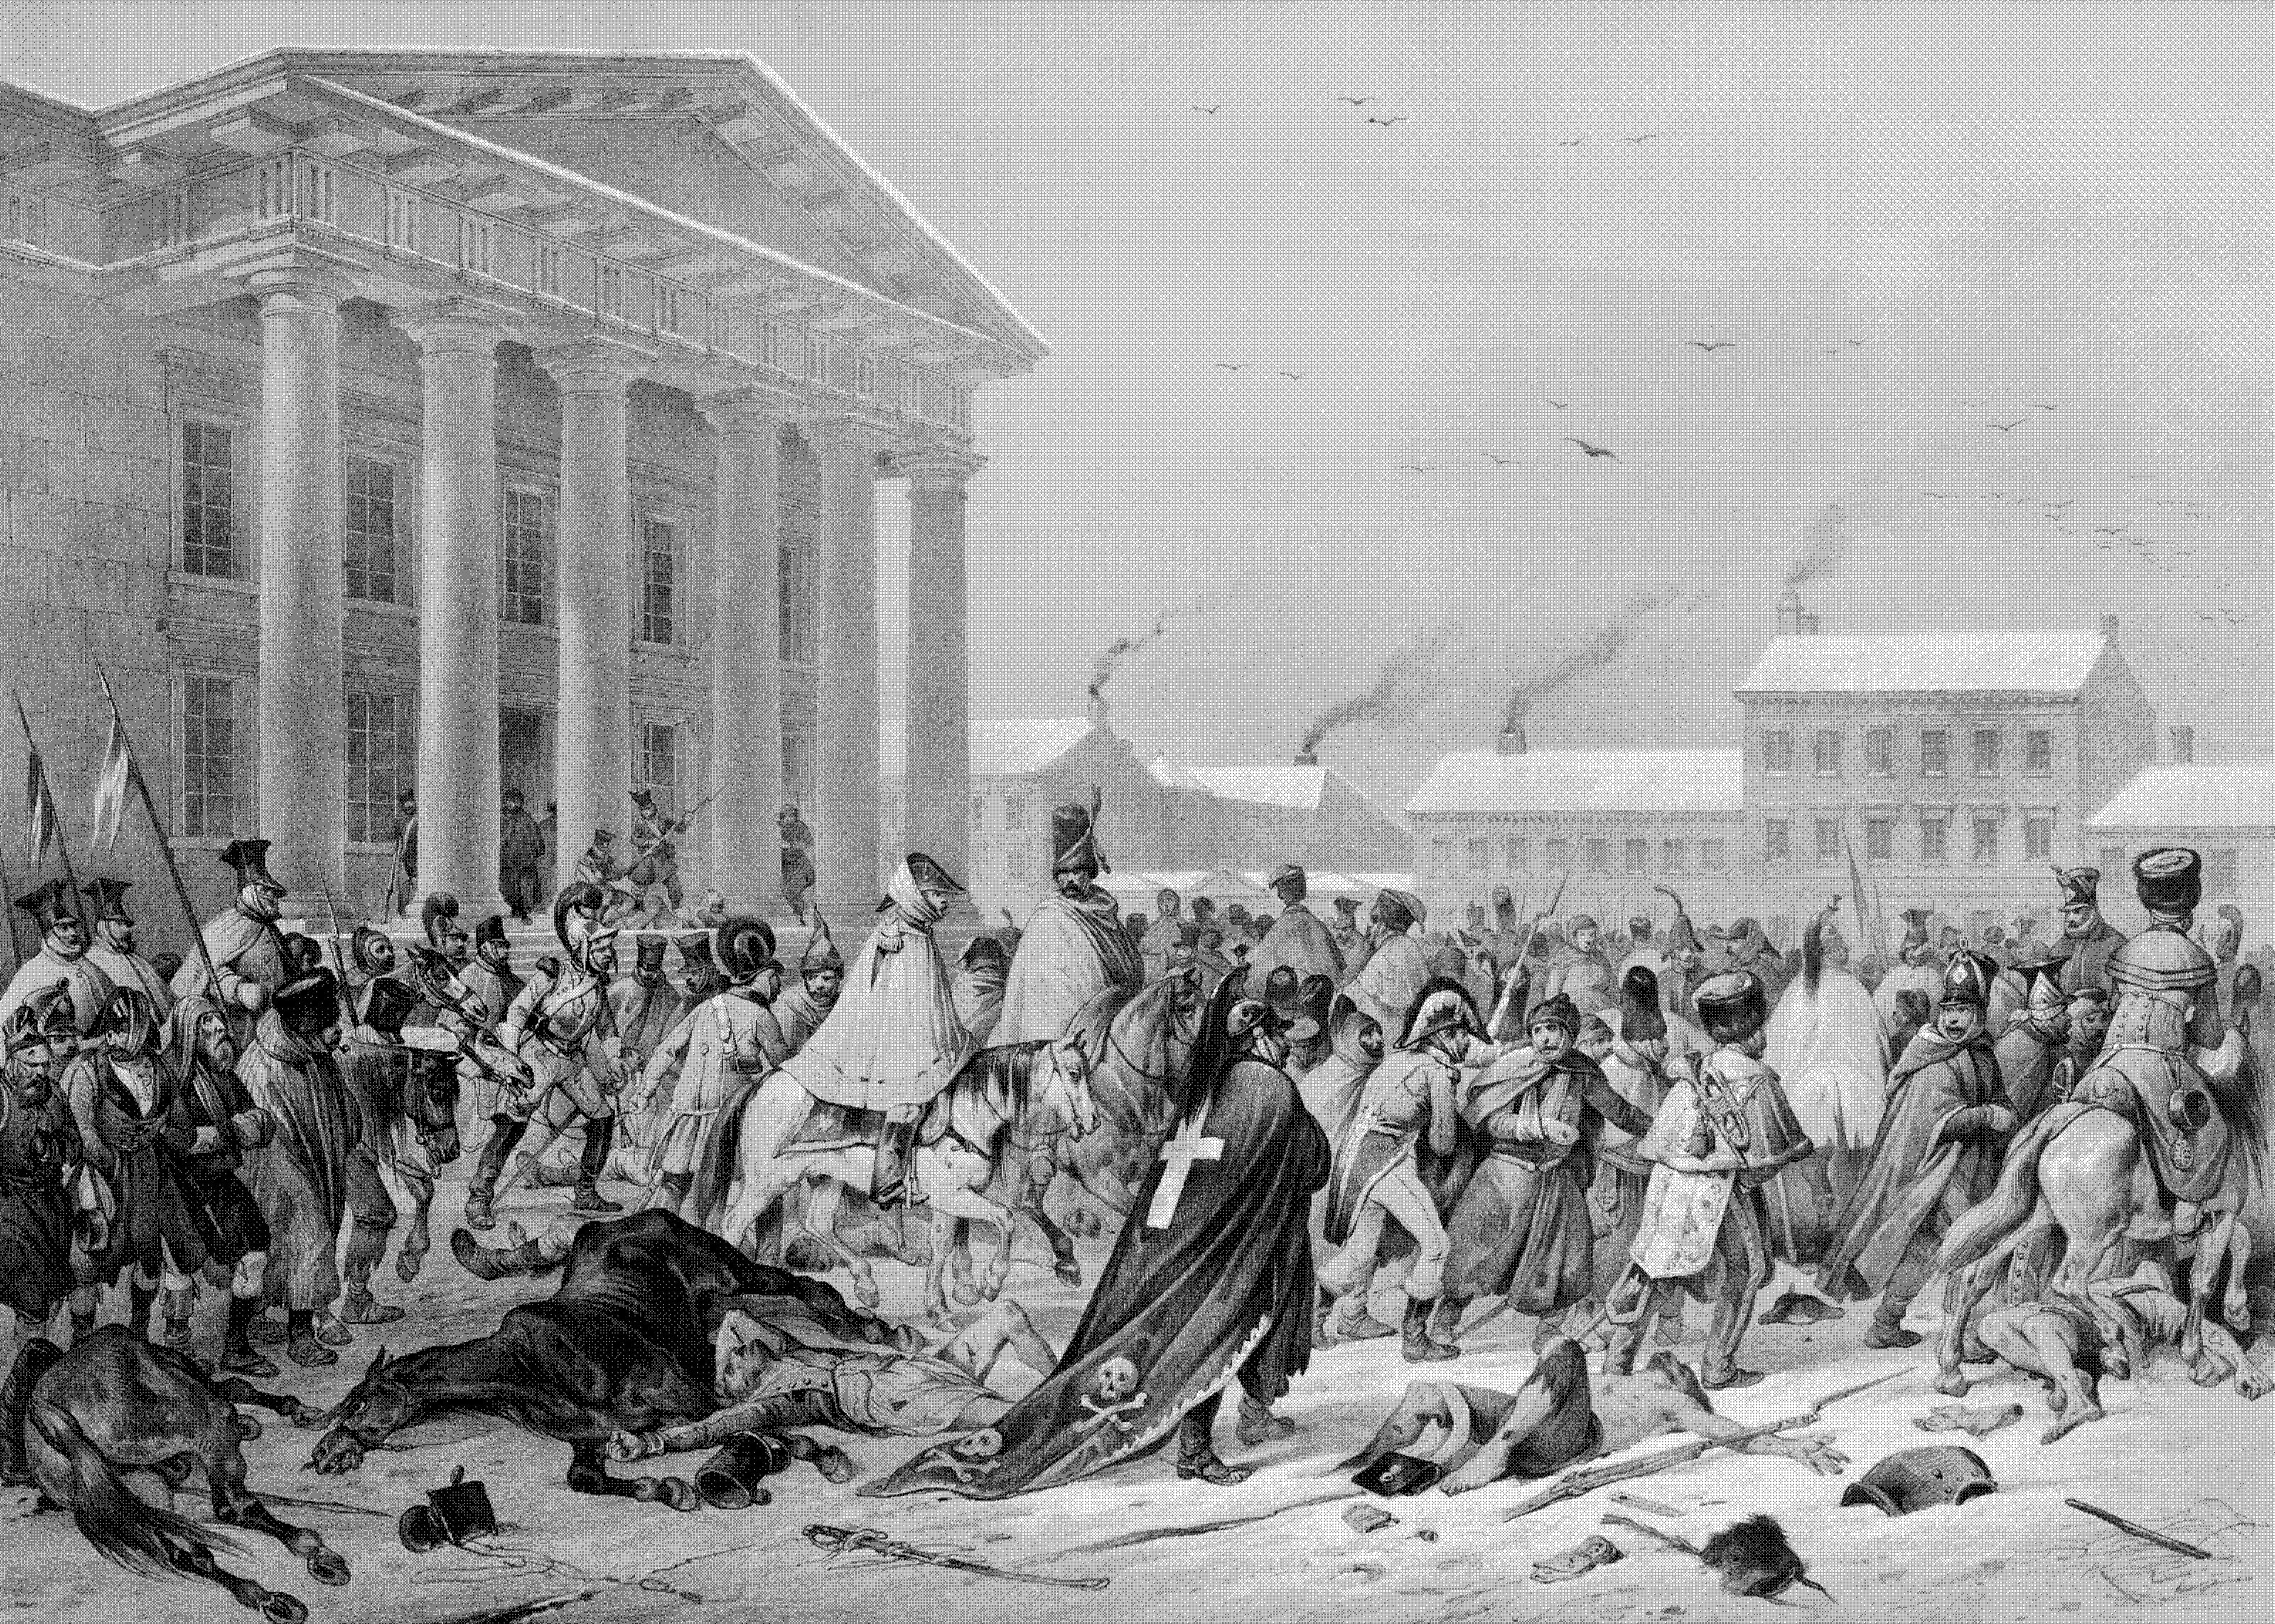
\includegraphics[width=\textwidth]{ilustra-06.png}
    \caption{Retrato de 1812 da Grande Armée em Vilna, a partir da pintura de J.\,Damel.}
\end{figure}

A incapacidade de Forster para aprender polonês (na variante local) fez
sua vida em \textit{Wilna} menos comunicativa. Embora se esperasse que desse
aulas em polonês, ele continuou suas instruções na universidade em
latim, que nem ele ou seus estudantes conheciam bem. Em pouco tempo, o
naturalista transformou sua frustração linguística num ódio por tudo o
que fosse polonês. Ele até mesmo decidiu evitar que a filha, nascida
logo após a chegada de Therese a \textit{Wilna}, ouvisse aquela língua. ``Espero
que minha filha não venha a precisar do conhecimento do idioma polonês,
embora devamos ficar aqui por sete anos. Mas mesmo que sua língua se
torne mais flexível, isso não compensaria o dano potencial que longas
conversas em polonês com diversos nativos ignorantes, padres locais e
outros idiotas infligiriam em sua mente.''\footnote{Forster escreve para Sömmerring, 8 de outubro de 1786, \textit{Georg Forsters Werke 14}, op. cit., p. 561.}

Forster demonstrou ainda menor interesse pelo lado (mais vasto) judaico
da cidade. Ele com frequência fundia negativamente os dois universos num
só, sobretudo em questões de comércio local, que descreveu como
``completamente dominado por cristãos com virtudes judaicas''\footnote{Georg Forster escreve para Johann Karl Phillip Spener, 17 de junho de 1787, ibid., p. 699.} que cobram preços \textit{unchristlich}, ou ``não"-cristãos'',\footnote{Forster escreve para \textsc{t}.\,Heyne, 16 de fevereiro de 1785, ibid., p. 282.} por serem ``mais gananciosos que os hebreus.''\footnote{Forster escreve para Sömmerring, 12--13 de dezembro de 1784, ibid., p. 236.} Contudo, uma das poucas pessoas que Forster chegou a respeitar em \textit{Wilna} foi um médico judeu com quem partilhou a
descoberta do filósofo judeu alemão Moses Mendelssohn.\footnote{O médico foi provavelmente Judah ben Mordechai ha"-Levi Hurwitz, embora Forster jamais mencione seu nome na correspondência.} O professor alemão participava de um pequeno salão filosófico organizado regularmente na
casa do médico. Costuma dizer que o ambiente iluminista se devia à
anfitriã, esposa do médico. Apesar de sentimentos cordiais, os Forsters
jamais se tornaram amigos próximos desse casal de judeus.

\asterisc

A Lituânia, em geral, constituía um estranho desafio representacional
para Forster, não por ser um ``país infeliz governado por uma tenaz
anarquia'', mas porque, em suas próprias palavras, ele era obrigado a se
utilizar de ``cores e metáforas completamente diferentes'' a fim de
capturá"-lo.\footnote{Georg Forster escreve para Petrus Camper, 7 de maio de 1787, \textit{Georg Forsters Werke 14}, op. cit., pp. 677--680.} Por conseguinte, Forster estava continuamente em busca de uma visão
descritiva perfeita que fosse capaz de transformar magicamente a caótica
cena lituana num quadro ordenado. Ao final, ele concluiu que a Lituânia
se encontrava presa entre dois polos contrastantes de desenvolvimento
cultural:

\begin{quote}
É possível identificar um farto material risível nessa mistura de
brutalidade sarmácia ou quase neozelandesa e de extremo refinamento
francês\ldots{} ou talvez não; pois damos risada apenas de pessoas cuja
única culpa é serem risíveis; não damos risadas daqueles que, por meio
das maneiras de governar, da pecuária (como a educação aqui deveria se
chamar), do exemplo, dos padres, do despotismo de vizinhos poderosos e
de um exército de vagabundos franceses e inúteis italianos, são mimados
desde a juventude, vendo"-se desprovidos de qualquer expectativa futura
de aperfeiçoamento. A verdadeira população, isto é, milhões de cabeças
de gado sob forma humana, aqui perfeitamente excluída de qualquer
privilégio da humanidade\ldots{} a população está, atualmente, de fato,
graças a uma longa e costumeira escravidão, mergulhada num tal grau de
bestialidade e insensibilidade, de uma preguiça indescritível e de uma
ignorância tão estúpida, que talvez um século não seja suficiente para
que galguem ao mesmo nível da gentalha de outras nações
europeias.\footnote{Georg Forster escreve para Georg Christoph Lichtenberg, 18 de junho de 1786, ibid., pp. 491--492 [Tradução para o inglês por Wolff, op. cit., p. 338].}
\end{quote}

Forster, auto"-intitulado especialista em raças humanas, não mostrava o
mínimo interesse pela localização cultural intermediária da Lituânia
como universo entre civilização e selvageria. Ao invés de observar em
derredor e encontrar algo novo ou interessante na natureza lituana
(assim como dele esperavam seus colegas), ele se ensimesmou,
concentrando"-se em seu próprio desenvolvimento. No jargão naturalista,
ele descreveu sua existência em \textit{Wilna} como a de uma larva pronta para
deixar o casulo e esticar as asas.\footnote{Forster escreve para Sömmerring, 3 de fevereiro de 1785, ibid., p. 271.} Numa terminologia mais clássica, ele lhe deu o nome de \textit{Ulubris
Sarmaticis}.\footnote{Forster escreve para Herder, 21 de julho de 1786, ibid., p. 512.} Na Antiguidade, Ulubris era uma cidade remota onde, alegadamente, o primeiro imperador romano Augusto (Otávio César) passou
a adolescência antes de ser adotado pelo tio"-avô Júlio César. Era um
lugar de exílio, mas também de antecipação, e Forster ansiava por um
indulto real que o resgatasse. Como sempre, sua esposa era mais
pragmática. ``Nosso clima é rigoroso'', escreveu Therese, ``o ambiente é
duro e infértil; a comida, em geral, é barata, mas ninguém tem preço
fixo. A nação é asselvajada e seus nativos não pertencem à humanidade.
Mas chega de falar deles; sinto pena deles, porém não vejo a hora de me
tornar uma leal súdita da Rússia, Áustria ou Prússia, assim que
recomeçar a próxima partilha deste país.''\footnote{Therese Forster escreve para Spener, 19 de fevereiro de 1786, ibid., p. 793.} Ambos os seus desejos se tornaram realidade.

No verão de 1787, o embaixador da Rússia abordou Forster com uma oferta.
O almirantado russo planejava uma expedição ao redor do mundo, incluindo
uma vasta investigação científica da costa do Oceano Pacífico na Ásia e
América do Norte. Forster foi recomendado à função de cientista"-chefe da
viagem, garantindo"-se"-lhe liberdade irrestrita de pesquisa e uma
recompensa financeira substancial. Ele se entusiasmou com a oportunidade
de ir ``para além do Japão e Kamchatka'', e avisou Herder de imediato
quanto à possível saída da Sarmácia: ``Caríssimo e amado amigo! [\ldots{}]
Você talvez tenha tomado conhecimento de que, graças ao \textit{Deux ex
machina}, fui libertado de meu \textit{pontus Wilna}\foonote{No original, \textit{Wilnaschen
Pontus}.} e, na qualidade de súdito russo, participarei de novo de uma
expedição aos mares do Sul.''\footnote{Forster escreve para Herder, 1 de setembro de 1787, \textit{Georg Forsters Werke 15}. Berlim: Akademie Verlag, 1981, p. 32.} Havia, contudo, um sério obstáculo aos planos de Forster --- o senado da universidade não queria
liberá"-lo do contrato de sete anos. A tzarina russa Catarina \versal{ii}
interferiu e, por intermédio do ex"-amante, o rei polonês Stanislaw
Poniatowski, ela comprou o contrato de Forster com a universidade.

Os Forsters saíram de \textit{Wilna} no fim do verão de 1787. O naturalista foi
para Londres, e sua esposa, para a casa dos pais na Alemanha. Enquanto
isso, eclodiu uma guerra entre a Turquia e a Rússia, de modo que a
expedição teve de ser adiada por tempo indeterminado. Em Londres,
Forster recebeu o pedido de reassumir a posição de docente na
universidade de \textit{Wilna}, mas, desligado das obrigações financeiras, ele se
recusou em voltar para o ``exílio''. Outrossim, ficou encantado em
saber"-se ainda necessário nas florestas periféricas da Sarmácia:

\begin{quote}
Minha felicidade aumenta a cada dia ao receber tantas cartas da Polônia.
Desde que a expedição ao redor do mundo foi cancelada, tenho recebido
pedidos para retornar a \textit{Wilna}. Sou desejado pela universidade local, que
me pede que apresente minhas condições contratuais. Devo admitir que
isso não só é prazeroso, como é também o momento do meu triunfo, a única
vitória capaz de satisfazer qualquer indivíduo honesto e determinado.
Antes, fui desprezado por ter partido; agora, estão ávidos por
recompensar minha diligência convidando"-me de volta da maneira mais
honrosa. Tal pedido dobra minha satisfação, pois não tenho necessidade
de retornar. Uma vez na vida \textit{Wilna} cai bem, mas nunca duas vezes.
Acredito ter cumprido meus deveres com responsabilidade, e todos se
satisfizeram comigo; mas não fiquei contente com a situação. Deveria
estar feliz pelo tempo que lá passei\ldots{} um homem solteiro talvez se
contentasse, mas um homem casado deve se preocupar com a felicidade da
esposa e a educação do filho. Ademais, rejubilo"-me em saber que minha
cátedra ainda está vaga e que a universidade não consegue encontrar
ninguém mais adequado que eu.\footnote{Georg Forster escreve para Johann Georg von Zimmermann, 4 de maio de 1788, \textit{Georg Forsters Werke 15}, op. cit., p. 151.} 
\end{quote}

%{[}figura 25{]}
%
%Panorama do jardim botânico da universidade. O jardim foi instituído
%pelo sucessor de Forster, o professor S.\,B. Jundzila, poucos anos depois
%de o naturalista alemão deixar a Lituânia.

Com o passar dos anos, sua esperança de que a expedição pelo Pacífico
fosse retomada diminuiu, e Forster canalizou suas aspirações para as
promessas da emancipação universal humana oferecida pela Revolução
Francesa. Chegou a Paris no auge da euforia revolucionária como delegado
junto à Assembleia Nacional, representando os territórios alemães
capturados pelos franceses. Num movimento, porém, em que os próprios
revolucionários de sangue francês podiam se tornar suspeitos, a origem
germânica mista de Forster empurrou"-o perigosamente para as margens da
revolução. Aos trinta e nove anos de idade, em 10 de janeiro de 1794,
Forster morreu de pneumonia em Paris, durante os piores meses do Terror.
Sua doença e morte prematura certamente o salvou da guilhotina. Mas
morreu na solidão. Abandonado pela esposa distante e pelo próprio pai,
ostracizado pela maior parte de seus compatriotas alemães e quase
totalmente esquecido pelos camaradas revolucionários franceses, Forster
faleceu desesperado em seu ``porto seguro de resignação.''\footnote{Forster conforme citado em Saine, op. cit., p. 147.} Até mesmo o humanista Goethe, que havia se tornado amigo de Forster alguns anos antes e que
muito apreciava sua mente crítica, expressou não mais que uma reservada
simpatia por ocasião de sua morte em Paris. ``O pobre Forster,
portanto,'' lamentou o célebre escritor, ``teve que pagar, no final das
contas, com a própria vida pelos seus erros, mesmo que tenha escapado de
uma morte violenta! Sinceramente tive pena dele.''\footnote{Goethe escreve para Sömmerring, 17 de fevereiro de 1794, conforme citado em Saine, op. cit., p. 155.}

A morte de Forster em Paris coincidiu com o desmembramento político da
Sarmácia. Em 1793, a Rússia e a Prússia procederam à segunda partilha da
Polônia"-Lituânia, provocada pela adoção da constituição liberal da
República em 1791. Em 1792, durante a invasão russa da Polônia"-Lituânia,
o exército tzarista ocupou a capital lituana. Em 24 de abril de 1794,
rebeldes locais liberaram Vilna e fundaram um comitê revolucionário
lituano. Tropas russas sitiaram a cidade até os rebeldes capitularem
quatro meses depois. A derrota da rebelião conduziu à partilha final da
República em 1795, que fez de Vilna uma cidade russa de província.

%{[}figura 26{]}
%
%Apagando a Sarmácia do mapa da Europa. A alegoria representa três
%governantes iluministas --- Catarina \versal{II} da Rússia (com o ministro do
%exterior Nikita Panin), José \versal{II} da Áustria e Frederico \versal{II} da Prússia ---
%procedendo à primeira partilha da Polônia"-Lituânia em 1772.

\chapter{A praga de Napoleão}

%\setlength{\epigraphwidth}{.45\textwidth}
\begin{epigraphs} 
\qitem{Em 1789, a fermentação se levanta em Paris; ela cresceu, transborda e se
exprime por meio do movimento dos povos do Ocidente para o Oriente.
Várias vezes, esse movimento se dirige para o Oriente, entra em choque
com um movimento contrário, do Oriente para o Ocidente; em 1812, ele
alcança seu limite máximo --- Moscou ---, e com uma simetria notável ocorre
um movimento contrário, do Oriente para o Ocidente, carregando consigo
os povos centrais, exatamente como ocorrera no primeiro movimento. O
movimento contrário alcança, no Ocidente, o ponto de partida do primeiro
movimento --- Paris --- e se aquieta.}{\textit{Guerra e paz}, \textsc{liev tolstói}\footnotemark}
\end{epigraphs}

\footnotetext{Conforme tradução feita por Rubens Figueiredo de \textit{Guerra e paz}, São Paulo: Cosac Naify, 2011. [\textsc{n.\,t.}]}

Em 11 de setembro de 1804, na véspera do dia do Santíssimo Nome de
Maria, um dos melhores médicos de Viena, 
Johann Peter Frank, deixou sua
casa rumo à cidade russa de Vilna. O doutor Frank estava acompanhado do
filho, Josef Frank (também médico), da nora --- uma 
elegante e talentosa cantora lírica italiana, chamada Christine Frank,
nascida Gerhardi --- das
duas filhas solteiras, Carolina e Lizete, e da governanta Frau Janisch.
Além deles, três pajens homens, uma camareira e um cozinheiro
engrossavam a grande família. O velho Frank transferiu ao filho as
responsabilidades da viagem pelas perigosas veredas de uma Europa em
guerra, e acabou se tornando a primeira vítima da estrada: depois de uma
noite fria ao relento, pegou um resfriado e teve que ficar de cama por
uma semana. No fim de setembro, a caravana finalmente chegou à Lituânia,
no posto de fronteira do rio Bug, onde as três grandes potências
europeias --- Rússia, Áustria e Prússia --- haviam estabelecido uma nova
fronteira após a divisão da Polônia"-Lituânia.

``Em Tiraspol,'' recordou Josef Frank, ``dissemos adeus ao reino
austríaco. Após atravessar o rio Bug, chegamos a Brest"-Litovsk; os
cossacos muito gentilmente nos abriram os portões do império russo.
Havia visto esses cossacos barbudos alguns anos antes, quando o exército
russo conduzido por Suvorov estacionou perto de Viena {[}em 1799{]}, e
sua estranha aparência não me surpreendera em nada. Percebera logo
também que esses cossacos não são tão cruéis como se pode imaginar. Na
verdade, eram mais razoáveis que a maioria dos oficiais de alfândega
russos.''\footnote{Jozefas Frankas (Josef Frank), \textit{Atsiminimai apie Vilnių}, trad. Genovaitė Dručkutė. Vilna: Mintis, 2001, p. 42.} O império russo também agradou aos viajantes pela efetiva demarcação das
estradas. ``Tão logo entramos na Rússia, ficamos muito surpresos com os
postes cuidadosamente pintados de verde que marcavam cada versta e
indicavam com precisão as distâncias entre a fronteira e as duas
capitais russas {[}São Petersburgo e Moscou{]}. Uma vez que sete verstas
correspondem aproximadamente a uma milha alemã, achamos estranho que o
maior império do mundo utilizasse as menores unidades de medida
geográfica.''\footnote{Ibid., p. 44.}

As indicações de fronteira e de direção, recém"-pintadas, eram sinais de
uma nova era. Ao concluírem as três partilhas (em 1772, 1793 e 1795) da
República Polono"-Lituana, os monarcas russo, austríaco e prussiano deram
início a um período de rearranjamento territorial jamais visto. O
desmembramento da República foi apresentado pelos regimes absolutistas
como um gesto benéfico e necessário do espírito iluminista: a ordem
imperial substituía a anarquia sarmácia. Um espírito juvenil expulsava
uma era de tradições. Como bem observou Frank, na Rússia governada pelo
jovem tzar Alexandre \versal{i}, que subira ao trono em 1801, ``as mudanças
aconteciam a toda hora. Jovens impérios, como a Rússia, distinguem"-se
totalmente das velhas monarquias. Experimentam"-se continuamente novos
métodos administrativos, tornando cada ano diferente do anterior. Uma
nova ordem substitui a antiga, conduzindo a sociedade local de um
sistema para outro. No império russo, onde tudo muda a cada minuto, a
única certeza é a própria instabilidade.''\footnote{Ibid., p. 46.} Nem
mesmo a forma tzarista de originalidade política, mudança cultural e
flexibilidade social, contudo, era capaz de competir com as ambições
continentais de Napoleão, que se nutria da ebulição incontrolável das
ruas parisienses, transformando"-a num eficiente instrumento de
governança inspirado por ideais revolucionários e lucros baseados na
guerra. A fantástica ascensão de Napoleão às alturas imperiais tornou
obsoleto qualquer mapa da Europa. Sob a pressão do exército francês e
dos revolucionários locais, velhos estados sucumbiram como nunca antes,
ao passo que novos estados, decorados com nomes da Antiguidade ou novos
rótulos (tais como Etrúria, Helvétia, Ilíria e Batávia, ou a República
Cisalpina e a Confederação do Reno), foram criados da noite para o dia
ao toque veloz da pena do conquistador. A Europa, junto com a família
Frank, estava em movimento, transformando seu velho estilo de vida rumo
a um novo início.

A família Frank, contudo, logo se deu conta de que viajar pelo terreno
de um império em transformação não era menos desafiador que perambular
pela caótica Sarmácia. A estrada recém"-cartografada era despopulada e
desprovida dos confortos mais elementares. ``Avançávamos tão rápido
quanto possível pelas estradas arenosas da Lituânia. A floresta sem fim
que atravessávamos tinha um quê de majestade. Mas os campos congelados
que se entreviam entre os bosques pareciam nos dizer que o inverno já
havia chegado. O vento setentrional, também, soprava como um lembrete
adiantado. Viajávamos noite e dia sem encontrar abrigo ou comida.
{[}\ldots{}{]} A fome azedou nossa gloriosa chegada a Vilna, que
adentramos em 4 de outubro de 1804, às dez e meia da manhã.''\footnote{Ibid., pp. 44--45.} Exatos dois meses depois, em Paris, Napoleão haveria de se coroar imperador.

Vilnius, ou como os russos e franceses a chamavam, Vilna, tornara"-se a
terceira maior cidade do império russo, depois de São Petersburgo e
Moscou. A população total do (antigo) Grão"-Ducado da Lituânia era de
cerca de quatro milhões e meio de habitantes; o recenseamento efetuado
em 1795 indica 17690 moradores de fé cristã morando na cidade. Entre
seus residentes, havia 2471 membros da nobreza, 568 padres católicos e
107 sacerdotes de outras confissões, 238 professores e acadêmicos e 860
artesãos organizados em 38 corporações de ofício. As autoridades russas
listaram ainda 32 igrejas católicas, 15 mosteiros, 5 igrejas
greco"-católicas com 3 mosteiros, uma igreja ortodoxa russa, uma igreja
luterana e uma igreja reformista (calvinista), além de 10 grandes
palácios.\footnote{Tomas Venclova, \textit{Vilnius: City Guide}. Vilna: \textsc{r}.\,Paknio leidykla, 2001, p. 37. O recenseamento de 1795 não fornece estatísticas sobre residentes de confissões não"-cristãs.} A população judaica local --- talvez a maior parte de seus habitantes --- fora
simplesmente deixada sem contar pelos burocratas tzaristas. Frank, em
suas memórias de Vilna, imbuiu o quadro estatístico da cidade com
detalhes mais vívidos:

\begin{quote}
Vilna tinha um aspecto caótico --- inúmeros palácios rodeados por
choupanas. Embora houvesse muitos edifícios feitos de tijolos, a maior
parte das casas eram de madeira. Abaixo da Colina do Castelo, a porção
da cidade que se estendia ao longo da confluência dos dois rios era
extremamente suja. O admirável prédio da prefeitura, em estilo italiano,
se erguia numa praça bela e ampla, repleta de barracas horrendas de
incontáveis comerciantes. As ruas que conduziam à majestosa catedral,
não pavimentadas e cheias de lixo, logo se transformavam num lamaçal
sempre que chovia. Porcos corriam por toda parte e, do lado de fora da
cidade, tudo o que se podia notar com os olhos e o nariz eram enormes
montes de estrume. Os subúrbios literalmente afundavam em areia e
sujeira, algo que nem mesmo a beleza natural da paisagem circundante era
capaz de ocultar.\footnote{Frank, op. cit., p. 49.}
\end{quote}

Apesar da aparência deplorável, a cidade detinha a aura de uma cosmópole
da Antiguidade. ``A capital lituana,'' continua Frank, ``tinha mais de
35 mil habitantes: entre eles, havia cerca de 22 mil católicos, 600
ortodoxos gregos, 500 luteranos, 100 reformados, 11 mil judeus e 60
muçulmanos. A aristocracia local, professores universitários e burgueses
eram católicos em sua maioria. Entre os ortodoxos gregos, havia
autoridades do governo, comerciantes e agricultores russos. Os luteranos
e calvinistas (alemães em sua maioria) estavam envolvidos em atividades
artísticas, de artesanato e comércio.'' Os judeus ``compunham uma
comunidade separada'' cuja história local ``perdia"-se no tempo.'' A
população judaica chegou à Polônia ocidental vindo da Alemanha, mas,
observa o médico, ``à parte oriental do país {[}Lituânia{]}, eles vieram
da região do Mar Cáspio. Outros especialistas incluem também os caraítas
como judeus, mesmo que não falem um idioma de influência alemã. Na
Lituânia, porém, os judeus de origem alemã\footnote{A referência feita diz respeito aos judeus \textit{ashkenazi}.} muito diferem
de seus compatriotas da Alemanha: em Vilna, eles se vestem como Don
Basílio em \textit{O barbeiro de Sevilha}. As mulheres judias se vestem
exclusivamente à moda oriental, mas seus trajes --- valiosos ou não ---
estão quase sempre imundos.''\footnote{Ibid.}

A família Frank se adaptou bem ao mundo imperial dessa metrópole de
província. Pai e filho se mudaram para Vilna a convite de Alexandre \versal{i}, a
fim de dirigir a Faculdade de Medicina da universidade local.
Rapidamente, o velho Frank foi chamado para São Petersburgo para se
tornar o médico particular da família do tzar, enquanto o filho ficou em
Vilna por quase duas décadas. (Durante sua longa e aventurosa vida, o
velho Frank teve o privilégio e o desafio de servir como conselheiro
médico para três famílias imperiais da Europa: Habsburgo, Romanov e
Bonaparte). Em 1803, a Universidade de Vilna foi reestruturada e
modernizada uma vez mais. Sob os auspícios do aristocrata polono"-lituano
Adam Jerzy Czartoryski (1770--1861), curador do Distrito Escolar Lituano,
amigo próximo e conselheiro"-chefe do tzar, a universidade foi
transformada numa academia europeia progressista. Durante as duas
décadas da direção de Czartoryski, ``que enfrentou a turbulência do
colapso de Napoleão e o período de ajustes pós"-napoleônico, \textit{Wilno}
empunhou a tocha da cultura polonesa, resgatando muitos dos ideais da
antiga Comissão Educacional e espalhando sementes para a mais brilhante
colheita intelectual do século.''\footnote{Norman Davies, \textit{Heart of Europe: the Past in Poland's Present}. Oxford: Oxford University Press, 2001, p. 173.} Apesar do caráter nacional polonês, a universidade recebeu o título de Universidade Imperial e se tornou uma
academia de ponta na Rússia. Os dois Frank, pai e filho, se gabavam de
ser suas brilhantes estrelas científicas.

%{[}figura 28{]}
%
%A Universidade Imperial de Vilna na primeira metade do século 19.

O jovem Frank nascera em 1771 e concluíra os estudos universitários em
Göttingen, embora houvesse passado a maior parte da juventude na Itália,
onde acabou conhecendo a esposa. No pequeno mundo da elite acadêmica
europeia, as trilhas profissionais das famílias Frank e Forster se
cruzaram com frequência. Embora a família Frank estivesse perfeitamente
a par da vida desafortunada, duas décadas antes, que Forster levara em
\textit{Wilna}, bem como de sua trágica morte em Paris, ela não comungava da
mesma posição melancólica para com a Lituânia, nem de seu zelo
revolucionário. Os membros da família Frank eram autênticos burgueses
vienenses: encaravam os prazeres da vida com gosto. Por intermédio da
esposa, o jovem Frank se ligou ao meio teatral e musical europeu e suas
casas, tanto a de Viena como a de Vilna, estavam sempre abertas aos
frequentadores dos mundos artístico e acadêmico.

%{[}figura 29{]}
%
%Cena de rua em Vilna.

A maior parte dos residentes de Vilna se opunham ao domínio tzarista, se
não de maneira aberta, pelo menos entre quatro paredes, de maneira que a
lealdade de Frank aos regimes imperiais russo e austríaco deveriam fazer
dele um estrangeiro mal quisto. A família Frank, entretanto, sediada em
sua confortável residência da Rua Grande, liderava os saraus da
cidade.\footnote{Ulteriormente, esse edifício do século \textsc{xvii} veio a ser conhecido como Casa Frank e, atualmente, abriga a Embaixada da França.} Isso se deveu, sem dúvida, à cordialidade, etiqueta profissional e
sensibilidade cultural do casal de anfitriões. Frank era um médico bom e
não preconceituoso, com reputação de ser um cuidadoso praticante da
medicina moderna. Embora talvez enervassem alguns colegas e farmacistas
locais, seus princípios de diagnóstico e métodos terapêuticos lhe
valeram imensa popularidade entre os pacientes da elite de Vilna,
obcecados que eram por novidade. O médico também fazia avanços
charmosos, benevolamente arrogantes e maliciosos no seio da sociedade, o
que o tornou objeto de toda espécie de fofoca, obsessões amorosas e
demandas sociais. Sua esposa, Christine, era também uma diva sedutora:
uma \textit{prima donna} de um coração de ouro, que não só tolerava as
indiscrições do marido, como também desenvolvia uma brilhante carreira
só sua. Na provinciana Vilna, ela era um tesouro musical ítalo"-vienense
de magnitude europeia. Poucos anos antes da chegada da família à
Lituânia, Franz Josef Haydn compusera sua obra"-prima em matéria de
oratório, \textit{A criação}, especialmente para a voz de Christine. Após
a primeira apresentação pública da composição em 1799 em Viena, a
crítica a descreveu como uma beleza graciosa dotada da mais fabulosa de
todas as vozes de soprano. Malgrado o sucesso lírico na capital
\textit{habsbúrgica}, ela acompanhou o marido para Vilna, onde os dois procuraram
se beneficiar do universo local com responsabilidades partilhadas:
Christine organizava e se apresentava em recitais para as atividades
beneficentes do médico. Essa generosa colaboração derrotou qualquer
ressentimento local --- a família Frank se tornando os queridinhos da
sociedade, e seu salão constituindo o coração unificador de uma cidade
fraturada dos pontos"-de"-vista cultural e político.

Para a família Frank, a vida em Vilna oferecia um certo grau de
conforto. ``Não faltava comida na cidade,'' recorda o médico,
``especialmente no inverno, quando as estradas congeladas garantiam o
transporte de mercadorias. As carnes bovina e suína e a vitela eram da
melhor qualidade e duas vezes mais baratas que em Viena. Havia também
abundância de muito boa carne de pássaro, em especial frangos
suculentos. O mercado local geralmente exuberava em carne de caça e
pescado. As pessoas mais modestas comem sobretudo batata, repolho e
beterraba, ao passo que nas casas mais ricas serve"-se aspargo, couve de
Bruxelas e alcachofra. O pão e a cerveja eram excelentes; o vinho,
contudo, era muito caro e tinha de ser trazido de Riga.''\footnote{Frank, op. cit., p. 49.} Numa Europa volátil em tempo de guerra, o acesso ao abastecimento de comida barata não era uma questão menor, em especial
durante os anos do bloqueio continental napoleônico.

Em Vilna, cidade predominantemente católica e barroca, a família Frank
se sentiu em casa. Frank, ao contrário de Forster, ansiava por se
integrar no universo local. Ele primeiro aprendeu polonês e, em seguida,
russo. A família adotou um bebê abandonado (corria o boato de que se
tratasse de um filho ilegítimo do médico). Ulteriormente, durante visita
ao velho Frank em Viena, o menino se tornou companheiro de brincadeira
de Napoleão \versal{ii}, filho do deposto Napoleão e neto de Francisco I,
imperador da Áustria. Mesmo depois desse encontro com a progenitura
imperial, Frank insistiu que seu único filho recebesse uma educação
local --- católica e polonesa. O médico liberal, porém, ficou ligeiramente
chocado com a informalidade dos costumes religiosos locais:

\begin{quote}
Em Vilna, encontramos mais monges e freiras que em Viena. Para além da
catedral e das igrejas de São Casimiro e São João (que pertenciam à
universidade), todas as outras igrejas tinham diversos mosteiros como
proprietários. Era impossível assistir às missas populares na igreja
dominicana, sobretudo aos domingos, quando as pessoas constantemente
entravam e saíam, perambulando sem cessar pelos corredores,
cumprimentando, se beijando e fofocando em voz alta com amigos e
conhecidos. Havia também igrejas gregas, luteranas e reformistas
{[}calvinistas{]}, uma sinagoga e uma mesquita. Em geral, os católicos
não festejavam o sábado, pois era um dia de feira em que os camponeses
vendiam seus produtos. Por outro lado, os judeus respeitavam com rigor o
seu sábado e outros feriados religiosos. Naqueles dias, não procediam ao
comércio, nem que se lhes oferecessem todos os tesouros do mundo. Os
tártaros muçulmanos respeitavam escrupulosamente a sexta"-feira, seu dia
sagrado. Fiquei muito impressionado com a concórdia, e mesmo a
camaradagem, existente entre os membros de diferentes confissões.
Durante o jantar oficial pelo aniversário do imperador {[}Alexandre
\versal{i}{]}, oferecido pelo governador"-geral russo em seu palácio, pude
encontrar o bispo católico, o arquimandrita grego, o pastor luterano e o
ministro calvinista sentados à mesma mesa. Todos conversando prazerosa e
amistosamente entre si.\footnote{Ibid., pp. 49--52.}
\end{quote}

Frank, porém, não era indiferente à mutável estratificação étnica e
social da população da cidade. Quando a família se estabeleceu na
Lituânia, Vilna ``estava repleta de lojas sofisticadas, cujos donos eram
em sua maioria alemães que mantinham um estilo de vida opulento e que
logo foram à bancarrota. Com o tempo, os patrões alemães não conseguiram
mais competir com os comerciantes judeus, que levavam uma vida frugal e
se satisfaziam com lucros pequenos, podendo cobrar preços muito mais
baixos pelas mesmas mercadorias.''\footnote{Ibid., p. 50.} Durante os
anos das guerras napoleônicas, quando o contrabando e o comércio
clandestino floresceram, a competição mais desafiadora ao comércio dos
judeus surgiu com a política protecionista do estado russo e seus
corruptos representantes locais. ``Não devemos esquecer,'' recorda
Frank, ``que as esposas dos funcionários públicos russos do alto escalão
pegavam tudo o que queriam das lojas dos judeus, sem ao menos pensar em
pagar pelos produtos requisitados. Os comerciantes não podiam se queixar
às autoridades, pois, se fossem pegos com mercadoria contrabandeada,
necessitariam de proteção daqueles mesmos funcionários
públicos.''\footnote{Ibid.}

Frank foi um dos primeiros não"-judeus da cidade a entrar no bairro
judaico com um sentido de dever profissional. Para o médico, os judeus
de Vilna ofereciam uma oportunidade única para testar algumas das mais
recentes teorias de etnografia médica. À entrada do bairro judaico, ele
se imaginou viajando por terras exóticas, ou mesmo orientais:

\begin{quote}
Tão logo cheguei a Vilna, os judeus começaram a me procurar, pois eles
costumam sempre visitar um médico estrangeiro recém"-chegado. A prática
médica, entre os judeus, era muito lucrativa, porém as recompensas
financeiras não eram capazes de superar os aborrecimentos do ofício. Eu
tinha, contudo, um objetivo mais altaneiro. Queria estudar os hábitos e
o estilo de vida daquela misteriosa nação. Os judeus locais não deveriam
ser confundidos com os judeus de outras partes da Europa, onde mais ou
menos se pareciam com a população cristã. Os judeus poloneses não têm
nada a ver com eles. Então disse a mim mesmo: se tantos médicos têm de
empreender longas viagens cruzando oceanos a fim de estudar enfermidades
em terras exóticas e longínquas, eu não deveria temer perigos menores ao
tratar os judeus de Vilna. Após tal resolução profissional, já estava
pronto para entrar nos quintais escangalhados e cheios de lixo, galgar
as escadas precárias na direção dos apartamentos surrados e sujos, e me
expor a piolhos e a uma atmosfera insalubre.

De início, mal podia compreender a língua, uma vez que eles temperam o
idioma alemão com diversos vocábulos poloneses e hebraicos. Por outro
lado, os judeus poloneses me entendiam perfeitamente, embora não
parassem de fazer perguntas. Eu me irritava rápido em ter que repetir as
mesmas coisas o tempo todo. Mas logo percebi que precisava explicar"-lhes
tudo em detalhe: como tomar remédios e como seguir uma determinada
dieta. Funcionou! E então comecei a utilizar esse método de explicação
para todos os meus pacientes {[}judeus e não"-judeus{]}.

Devo admitir que os judeus poloneses cuidam muito bem de seus pacientes,
a quem nada falta. Sem dúvida, os judeus precisam cuidar de si mesmos
pois levam vida lutando constantemente contra diversas enfermidades.
Segundo os doutores Friedlander e Tainer, que compuseram monografias
médicas sobre as enfermidades dos judeus poloneses, a débil constituição
dos judeus é resultado de seu estilo de vida. Desde a mais tenra idade,
os judeus são obrigados a estudar intensamente as assim chamadas
escrituras religiosas, que no fundo não passam de uma espécie de
maluquice rabínica. Casam"-se muito cedo, na idade em que as crianças do
norte {[}da Europa{]} ainda estão na puberdade. E devemos ainda recordar
sua dieta inadequada, que consiste sobretudo em arenque e cebola; suas
estridentes cerimônias religiosas em sinagogas abafadas e mal
ventiladas; e a prática, entre as mulheres, de se lavar com água fria
após a menstruação e a cópula. Ainda por cima, eles praticam um jejum
rigoroso, respeitado estritamente por quase todos os judeus, e vivem em
condições insalubres. Não devemos também esquecer o tráfico ilegal de
mercadorias, que torna a vida dos judeus tão estressante, causando"-lhes
muitas enfermidades cardíacas; sofrem, ademais, com o comportamento
cruel para com eles por parte dos outros habitantes locais, da polícia e
do exército. Não aborrecerei o leitor com uma longa lista adicional de
detalhes sobre seu estilo de vida nada saudável. Outrossim, cumpre dizer
que os membros dessa nação preservaram uma compleição peculiar, quase
oriental, que os torna mais resistentes a certas patologias médicas. O
progresso de doenças crônicas, por exemplo, é muito menos variável entre
os judeus do que entre pessoas de outras nações, que, em geral,
necessitam de maior atenção e cuidado médicos. Em geral, os judeus
poloneses exemplificam várias hipóteses médicas de Hipócrates, sobretudo
no que toca às observações sobre o progresso da crise. O tratamento
médico dos judeus poderia se tornar mais interessante do ponto de vista
científico e mais benéfico do ponto de vista profissional caso
permitissem a autópsia \textit{post"-mortem}. Entretanto, os judeus da
Antiguidade aceitavam de bom grado o embalsamamento de seus
mortos.\footnote{Ibid., pp. 65--68.}
\end{quote}

O professor não logrou produzir um trabalho substancial sobre as
``condições clínicas'' dos judeus, mas sua tentativa de registrar e
sistematizar as ``enfermidades judaicas'' foi uma das primeiras no
sentido de racializar o conhecimento médico. Em pelo menos uma ocasião,
o interesse de Frank pelos corpos dos judeus foi guiado por objetivos
mais tentadores:

\begin{quote}
Um de meus pacientes, o negociante Simpson, estava doente de reumatismo
e apresentava sintomas epilépticos. Ele não ligava para as superstições
judaicas e permitia que sua bela esposa se vestisse segundo a moda
francesa, embora tivesse"-lhe dito de cobrir o cabelo conforme a tradição
judaica. Ela tinha a própria carruagem e era livre para sair em visitas
sociais; podia até mesmo flertar um pouco com os homens. Esse tipo de
liberdade fez do negociante um pária no seio da comunidade judaica e,
por ocasião de sua morte, a \textit{Kahal}, autoridade judaica comunitária, se
posicionou contra o sepultamento do cadáver no cemitério judaico. Os
judeus mais pobres estavam ávidos por profanar seu corpo, e \textit{madame}
Simpson entrou em pânico; felizmente, tudo terminou apenas em lágrimas.
Ela costumava me respeitar sem questionar e, certa vez, descobriu a
cabeça na minha frente. Foi um gesto de extrema intimidade, que admirei
mais do que qualquer outro gesto de reconhecimento. Como são
inteligentes as mulheres orientais, disse para mim mesmo, ao só
aparecerem em público embrulhadas em xales da cabeça aos pés!\footnote{Ibid., pp. 110--111.} \end{quote}

Na mesma época da chegada de Frank a Vilna, as ideias europeias sobre o
Oriente adquiriam novas conotações. O Oriente se tornara o quintal
marcial, mercantil e estético da Europa: não deveria apenas ser
conquistado, mas desvelado, seduzido e exposto. Os impérios europeus se
fizeram no Oriente, e Napoleão estava ansioso por obter seu mais
precioso troféu, a Índia. Ele via dois obstáculos em seu trajeto rumo à
Índia --- a marinha britânica e o expansionismo russo. Incapaz de
sobrepujar o primeiro, ele se concentrou no último.

Em 1807, no auge do triunfo militar, Napoleão assinou o tratado de paz
de Tilsit com Alexandre, às margens do rio Niemen. O tratado de paz
fortalecia o Sistema Continental e criava o Grão"-Ducado de Varsóvia a
partir do que restara do reduzidíssimo reino da Prússia. Embora a paz
entre França e Rússia houvesse prevalecido por algum tempo, ambos se
preparavam para uma nova guerra. Como Vilna ficara fora do Grão"-Ducado,
o ressurgimento de um estado polono"-lituano estava na cabeça de todos.
Na primavera de 1812, Napoleão começou a reunir uma quantidade imensa de
tropas com vistas à invasão da Rússia. Encarava a iminente guerra como
``sua `guerra polonesa' e, ao cruzar a fronteira do Império Russo, a
\textit{Grande Armée} estaria de fato restaurando a fronteira histórica da
Polônia e Lituânia, anulada em 1795.''\footnote{Davies, op. cit., p. 142.}

Para a família Frank, o ano de 1812 trouxe também mudanças
significativas. Pressentindo desconfiança e hostilidade --- afinal, a
Áustria estava do lado de Napoleão --- a família saiu de Vilna em maio de
1812, logo antes do início da campanha militar. Durante o período de
guerra, a família Frank permaneceu em segurança em Viena. Mas um
infortúnio atingiu Christine Frank: ela perdeu a voz diante de toda a
família imperial austríaca durante uma apresentação da ópera \textit{Le
nozze di Figaro} de Mozart, regida por Salieri. Sua voz retornou, mas
sem a força e o brilho de outrora. Jamais voltou a se apresentar.

\asterisc

Para sua guerra polonesa, Napoleão levou consigo os mais atualizados e
detalhados mapas da Lituânia, mas, em todo caso, escolheu também alguns
mapas da Índia.\footnote{Em geral, o exército francês parece ter tido uma compreensão geográfica e um conhecimento cartográfico parcos sobre a Lituânia. Contudo, antes do início da campanha russa, Napoleão se familiarizou com o trabalho de \textsc{c}.\,Malte"-Brun, geógrafo francês que, em 1807, publicou um estudo geo"-histórico sobre a Polônia, intitulado \textit{Tableau de la Pologne ancienne et modern}, que incluía também a Lituânia.} O imperador demonstrava uma compreensão cartográfica muito limitada da Rússia e, quando um de seus generais, Narbonne, indagou"-o
sobre as estratégias de guerra, ele simplesmente deu uma resposta
retórica: ``Que o destino se cumpra, e que a Rússia seja esmagada sob o
meu ódio pela Inglaterra! Liderando quatrocentos mil homens\ldots{} com
um batalhão lituano de gente do mesmo sangue da população que
atravessaremos, não temo esse longo trajeto margeado por desertos.
Afinal de contas\ldots{} esse longo trajeto é o trajeto rumo à Índia.
Alexandre, o Grande, partiu para alcançar o Ganges de uma distância que
não era maior do que a de Moscou. [\ldots{}] Seria uma expedição
gigantesca, admito, mas possível no século \textsc{xix}. Num só golpe, a França
terá conquistado a independência do Ocidente e a liberdade dos
mares.''\footnote{Paul Britten Austin, \textit{1812: the March on Moscow}. Londres: Greenhill Books, 1993, p. 31.} Nesse esquema grandioso de dominação global, Vilna era vista como um portão
para o Oriente.

A fim de garantir ``a independência do Ocidente,'' os seiscentos mil
homens da \textit{Grande Armée} se reuniram na margem esquerda do rio
Niemen, um rio lituano que, depois do remapeamento imperial da Europa,
se tornara a fronteira com a Rússia. A \textit{Grande Armée} --- o maior
exército jamais reunido na história da Europa --- era realmente uma
babilônia de nações:

\begin{quote}
Da direita para a esquerda, ou de sul a norte, o exército se enfileirou
ao longo do Niemen. No canto direito, vindo da Galícia, o Príncipe
Schwartzenberg com trinta e quatro mil austríacos; à sua esquerda, vindo
de Varsóvia via Bialystok e Grodno, o rei da Vestfália à frente de
setenta e nove mil e duzentos vestfálios, saxões e poloneses; mais para
a esquerda, o Vice"-rei da Itália, que havia mobilizado seus setenta e
nove mil e trezentos bávaros, italianos e franceses perto de Marienpol;
em seguida, o Imperador com duzentos mil homens comandados por Murat, o
Príncipe de Eckmuehl e os Duques de Danzig, Ístria, Reggio e Elchingen.
Essas tropas tinham marchado desde Thorn, Marienwerder e Elbling; e no
dia 23 de junho todas elas foram reunidas num só corpo compacto perto de
Nogarisky, a cerca de uma légua depois de Kovno.

Tudo estava pronto. Desde Guadalquivir e o litoral da Calábria até as
margens do Vístula, seiscentos e setenta mil homens (dos quais
quatrocentos e oitenta mil já estavam presentes), seis companhias de
engenheiros, um comboio de assédio, milhares de carroças de provisões,
inúmeros rebanhos bovinos, mil, trezentos e setenta e duas peças de
canhão, milhares de peças de artilharia e carroças"-hospital foram
agrupados e estavam agora estacionados a pouca distância do rio
russo.\footnote{Phillipe"-Paul de Ségur, \textit{Napoleon's Russian Campaign}, trad. \textsc{j}.\,David Townsend. Londres: Michael Joseph, 1959, pp. 16--17.} \end{quote}

O Conde Phillipe"-Paul de Segur, que descreveu esse impressionante
encontro da Europa napoleônica, seguia os passos do pai, que havia
atravessado a Lituânia rumo a São Petersburgo em sua missão diplomática
em 1784. Na França imperial, a dinastia Segur se aproveitou ao máximo de
suas origens no \textit{ancien régime}. O velho Segur havia servido como
Grão"-mestre de Cerimônias durante a coroação de Napoleão, e seu filho
participou da expedição de 1812 como Intendente"-Geral. O jovem Segur
venerava Napoleão e, como a maioria dos militares, sentia"-se seduzido
pela orientação e força ambiciosa da campanha. ``Através da escuridão os
nossos olhares ávidos se esforçavam por enxergar aquela gloriosa terra
prometida. Imaginávamos escutar os gritos jubilosos dos lituanos à
aproximação de seus redentores. No olho de nossa mente, víamos o rio
alinhado com mãos suplicantes. Aqui nada tínhamos, lá, seríamos cobertos
por dádivas\ldots{} {[}e{]} seríamos cercados por amor e gratidão\ldots{} O
dia surgiria por pouco tempo, trazendo calor e ilusões. [\ldots{}] O dia
realmente surgiu! E nos revelou apenas trechos estéreis de areia e
sinistros bosques negros. E então nossos olhos desenganados se voltaram
para nós mesmos, e sentimos como o orgulho e a esperança cresciam de
novo dentro de nós à visão impressionante de nosso exército
reunido.''\footnote{Ibid., p. 18.}

O Barão Louis"-François Lejeune, futuro retratista dos campos de batalha
napoleônicos, testemunhou esse tipo de orgulho do alto da colina em que
Napoleão organizou seu ponto de observação. Nas palavras do artista,
tratou"-se do ``mais extraordinário, mais pomposo, mais inspirador
espetáculo que se pode imaginar --- dentre todos, aquele que,
intensificando a extensão de seu poder, tanto material como moral, é
mais capaz de inebriar o conquistador. [\ldots{}] As saudações de milhares
de trompetes e tambores --- os gritos entusiasmados de aclamação ao
imperador sempre que aparecesse --- tanta devoção e disciplina prestes a
mover essa multidão cuja imensidão se perdia no horizonte, onde as armas
cintilavam como estrelas incontáveis --- tudo isso exaltava a confiança de
todos no chefe que nos liderava.''\footnote{Louis"-François Lejeune, \textit{Mémoires du Général Lejeune}, conforme citado em Austin, \textit{1812: the March to Moscow}, op. cit., p. 44.} Participantes menos imaginativos ou privilegiados da campanha, como o Locotenente
Heinrich August Vossler de Württemberg (que manteve um diário dos
eventos), viam a coisa a partir de um outro viés. ``Em 22 e 23 de junho,
uma verdadeira enxurrada de tropas finalmente avançou pela imensa
planície até as margens do rio que fazia fronteira com a Rússia, e lá
aguardaram a ordem de atravessar. Nos últimos dias, o exército francês
já tinha deixado atrás de si um rastro de pilhagem e destruição enquanto
se movia por território aliado. Só Deus sabe o que fariam em solo
inimigo!''\footnote{\textsc{h.\,a.}\,Vossler, \textit{With Napoleon in Russia in 1812: the Diary of \textsc{lt.\,h.\,a.}\,Vossler, a Soldier of the Grand Army 1812--1813}, trad. Walter Wallich. Londres: Constable, 1998, p. 45.}

Os primeiros sentinelas atravessaram o rio sem luta. Conforme as
memórias de Segur, apenas ``um oficial cossaco comandando uma patrulha
noturna'' apareceu na outra margem. ``Estava sozinho, parecendo pensar
estar em pleno período de paz, perfeitamente insciente de que diante
dele estava toda uma Europa armada. Perguntou aos invasores quem eram.
`Franceses,' responderam"-lhe. `O que vocês querem?' ele ainda indagou.
`E por que vieram até a Rússia?' No que um dos sapadores respondeu com
franqueza, `Para lutar contra vocês! Para tomar Vilna e libertar a
Polônia!'"\footnote{Segur, op. cit., p. 17.} Após o toque de batalha
das primeiras tropas, Napoleão atravessou o rio duas vezes no mesmo dia:
primeiro, envergando as cores francesas e, depois, vestindo o elegante
uniforme de hussardo polonês.

O único inimigo que as tropas libertadoras encontraram no caminho para
Vilna foi mandado pelos céus. A cidade fronteiriça de Kovno já havia
sido parcialmente destruída pelas forças russas em retirada. As tropas
libertadoras de Napoleão pilharam o que restara. ``Fogueiras ainda
fumegavam na praça do mercado, a mobília havia sido posta para fora das
casas e as vidraças, estilhaçadas. No máximo, era visto ainda um ou
outro judeu. Bastava um olhar. Kovno era uma cidade totalmente
saqueada.''\footnote{Carl von Martens, \textit{Dänkwürdigkeiten aus dem Leben eines alten Offiziers}, conforme citado em Austin, \textit{1812: the March to Moscow}, p. 57.} Depois de uma tranquila manhã, o céu repentinamente escureceu e emboscou a \textit{Grande Armée} com raios e
trovões. ``O céu ameaçador,'' relembra Segur, ``nesta terra sem abrigo à
vista, esmoreceu nosso espírito. [\ldots{}] A tempestade foi tão grandiosa
quanto nosso desígnio. Por várias horas, as nuvens se tornavam mais
espessas e mais negras por cima de todo o exército. De uma ponta a
outra, ao longo de cinquenta léguas, as tropas se encontravam por toda
parte ameaçadas pelos relâmpagos e submersas no aguaceiro. Estradas e
campos estavam alagados. O insuportável calor subitamente se transformou
num frio desagradável.''\footnote{Segur, op. cit., pp. 19--20.}

Com o imprevisível tempo lituano como principal adversário, o exército
avançou penosamente. ``Resumindo,'' escreveu Vossler, ``nossa situação
era a seguinte: vimo"-nos obrigados a proceder a uma árdua campanha
constituída por frequentes marchas forçadas ao longo de estradas
abomináveis, sufocados em areia ou chafurdados na lama até o joelho, ou
beirando precipícios sob um céu que alternava o calor insuportável com o
despejar de uma chuva gelada.''\footnote{Vossler, op. cit., pp. 50--51.}
A divisão de Vossler, pelo menos, seguia a estrada para Vilna --- a Guarda
Imperial de elite, atolada na intempérie, tinha se desnorteado. Um dos
veteranos da Guarda, o Sargento Bourgogne, lembra estar ``perdido, e
{[}eu{]} não sabia para que lado ir. Corri para me abrigar na direção do
vilarejo onde o General estava alojado, mas só tinha os relâmpagos para
me guiar --- de repente, durante um dos clarões, achei ter divisado uma
estrada (era infelizmente um canal, dilatado pela chuva até o nível do
chão). Esperando encontrar terra firme sob os pés, mergulhei e
afundei.''\footnote{Bourgogne, \textit{Memoir of Sergeant Bourgogne}, Londres: Jonathan Cape, 1940 {[}1896{]}, p. 16.}

A todos convinha culpar o mau tempo e o terreno traiçoeiro pelo retardo
do avanço. Numa escala maior, porém, a caótica marcha rumo a Vilna era
um sintoma da ignorância geográfica francesa sobre a região. Os mapas
franceses da Lituânia eram seriamente falhos: desatualizados, com
escalas inadequadas, e topograficamente incompreensíveis. A transcrição
ortográfica francesa dos topônimos lituanos era tão defeituosa que
impossibilitava a comunicação básica com a população local. Os moradores
locais simplesmente não podiam dar orientações porque não compreendiam a
pronúncia estrangeira dos nomes de suas próprias aldeias, vilarejos ou
cidades. De nada servira o fato de que o exército russo em retirada
removera todos os marcos de milha das estradas: ninguém parecia saber a
distância até Vilna, ou que direção o exército devia tomar. No
quartel"-general imperial, o conde polonês Roman Soltyk imediatamente
percebeu que ``a noção geográfica do império moscovita tida no gabinete
de Napoleão era tão imperfeita quanto possível, e o mesmo se aplicava ao
conhecimento topográfico. Todo tempo Napoleão interrogava continuamente
o general polonês Soholnicki a respeito desse assunto. Ao me dispor a
retificar a ortografia dos topônimos, mandaram"-me escrevê"-los direto no
mapa, de maneira que Napoleão pudesse ter uma ideia melhor de sua
localização.''\footnote{Roman Soltyk, \textit{Napoleon en 1812. Mémoires Historiques et militaires sur la Campagne de Russie}, conforme citado em Austin, \textit{1812: the March to Moscow}, p. 98.} Para o resto do exército, o sol, ao invés de um mapa, é que se tornou o guia mais
confiável na jornada para o leste. ``A cada dia,'' escreveu o General
Compans para sua jovem noiva: ``Estou me conscientizando da inadequação
dos mapas que temos, de maneira que comprei uma bússola para me guiar.
Embora não esteja acostumado a esse instrumento, não me falta a
esperança de que ele me possibilitará encontrar São Petersburgo ou
Moscou.''\footnote{Conforme citado em Austin, \textit{1812: the March to Moscow}, p. 98.}

Nesse meio tempo, a administração tzarista e a população local em Vilna
vinham também se preparando para a guerra. O quartel"-general do exército
russo, liderado pelo imperador, se localizava em Vilna. Desde o início
de junho, Alexandre e, junto com ele, a corte imperial russa (excetuando
os aposentos das senhoras), havia se mudado para o antigo palácio do
bispado, o qual, naquela altura, servia como residência oficial do
governador"-geral da Lituânia. Enquanto os preparativos de guerra
incluíam treinamentos e inspeções militares, a maior parte deles era
constituída por paradas intermináveis, procissões, torneios,
fiscalizações, festas de salão, banquetes, espetáculos teatrais,
concertos musicais e bailes extravagantes. Embora, em geral, a nobreza
local, em especial a geração mais jovem, tendesse a apoiar Napoleão, os
nobres lituanos se uniram de bom grado à corte imperial russa. Todos na
cidade esperavam que o tzar concedesse autonomia à Lituânia, como
contramedida às promessas de Napoleão de restaurar a antiga República.

%{[}figura 31{]}
%
%Polônia e Lituânia, ao redor de 1770. A maioria dos mapas utilizados
%pela \textit{Grande Armée} durante a campanha de 1812 retratava Vilna como
%poderosa fortaleza, mesmo que os últimos vestígios da muralha defensiva
%da cidade já houvessem sido destruídos pela administração russa.

Napoleão esperava uma batalha por Vilna, mas Alexandre lhe negou esse
prazer. Tão logo soube das notícias sobre o início da campanha, ele
abandonou a cidade rapidamente. As tropas e os funcionários públicos
russos logo o seguiram. Uma Vilna evacuada se preparou para a chegada da
\textit{Grande Armée}. Em 28 de junho, os lanceiros poloneses entraram na
cidade e foram saudados por uma multidão de patriotas. ``Nossa
entrada,'' lembra um dos participantes, ``foi um triunfo. As ruas e os
espaços públicos estavam abarrotados de gente. Todas as janelas estavam
enfeitadas com mulheres arrebatadamente entusiasmadas. As fachadas de
diversos edifícios ostentavam tapetes valiosos.''\footnote{Soltyk, op. cit., p. 71.} Uma ``imensa bandeira branca e azul"-celeste, alegadamente as cores {[}da dinastia{]} dos Jagiello, antigos soberanos
da Lituânia,'' foi alçada sobre as ruínas do antigo castelo do qual se
via toda a cidade.\footnote{François Dumonceau, \textit{Mémoires du Général Comte François Dumonceau}, conforme citado em Austin, \textit{1812: the March to Moscow}, p. 74.} Segur ecoa o mesmo sentimento: as pessoas na rua ``se abraçavam e se cumprimentavam. Velhos
se vestiam de novo com o antigo uniforme, com as memórias de honra e
independência. Choravam de alegria à visão das flâmulas nacionais
seguidas por multidões.''\footnote{Segur, conforme citado em Austin, \textit{1812: the March to Moscow}, p. 71.} Napoleão, desapontado, não demonstrava interesse por aquela exibição pública de alegria. Para ele,
tomar cidades provinciais era uma questão de importância estratégica;
assim, em primeira instância, ele queria saber tudo sobre as
características militares e topográficas do local. Antes de entrar na
cidade, o imperador francês mandou um emissário apanhar o reitor da
universidade, Jan Śniadecki, que era um idoso professor de astronomia e
meteorologia. Śniadecki assegurou diplomaticamente o imperador da
lealdade da cidade (e da universidade) para com ele e não para com sua
nêmesis imperial, Alexandre. Em troca, o reitor foi declarado membro do
governo provisório da Lituânia. Após a entrevista, segundo o General
Caulaincourt (ex"-embaixador francês na Rússia), ``o Imperador passou por
Vilna sem se fazer perceber. A cidade parecia deserta. Não havia um
único rosto numa vidraça sequer, nenhum sinal de entusiasmo ou mesmo
curiosidade. Tudo era sombrio. Ao passar no meio da cidade, ele
inspecionou a ponte Vilia, destruída pelo fogo, as áreas suburbanas e as
lojas que o inimigo havia incendiado e que ainda queimavam. Ordenou
pressa no reparo das pontes e na realização de obras defensivas, após o
que ele retornou e foi para o palácio.''\footnote{Armand de Caulaincourt, \textit{Mémoires du Général de Caulaincourt, Duc de Vizence, Grand Ecuyer de l'Empereur}, conforme citado em Austin, \textit{1812: the March to Moscow}, p. 73.} Num gesto de coragem, Napoleão ocupou os mesmos aposentos no mesmo palácio em que só dois dias
antes havia morado Alexandre. Com a substituição de uma corte pela outra
numa velocidade fenomenal, o papel de Vilna também se modificou. Antes
da invasão, ela era a assim chamada capital marcial da Rússia; agora,
era a primeira cidade da Europa napoleônica.

O medo talvez houvesse tomado conta da cidade, mas nenhum francês, o
imperador incluso, deixou de perceber a diferença no trato dos moradores
locais para com os poloneses e os libertadores estrangeiros: poloneses e
lituanos eram saudados como parentes, ao passo que franceses e outros
europeus eram perfeitos estrangeiros. Mesmo quando Napoleão estabeleceu
o quartel"-general imperial no palácio do governador"-geral russo e sua
chegada foi tornada pública, não houve festa na cidade. ``O Imperador,''
observou Caulaincourt, ``impressionou"-se com isso. Ao entrar em seu
gabinete, comentou: `Os poloneses daqui não são como os de Varsóvia. São
mais frios que os poloneses {[}em Varsóvia{]} e muito mais
reticentes.'"\footnote{Ibid.}

Apesar do sucesso estratégico, Napoleão não estava satisfeito com os
resultados táticos da ocupação francesa da cidade. Napoleão queria
humilhar Alexandre e, ao mesmo tempo, erigir uma estrada para o Oriente.
O recuo russo o aborreceu enormemente, pois privou"-o de uma inauguração
épica para a campanha. Ao receber uma carta de Alexandre, propondo a
negociação de um tratado de paz sob a condição de uma retirada imediata
da \textit{Grande Armée} para o outro lado do Niemen, Napoleão, conforme
Caulaincourt, se enfureceu:

%{[}figura 32{]}
%
%Palácio do governador"-geral em Vilna, onde Alexandre \versal{I} e Napoleão
%permaneceram durante a guerra de 1812.

\begin{quote}
Alexandre está brincando comigo. [\ldots{}] Como pode imaginar que vim até
Vilna para negociar acordos? Vim para aniquilar o colosso bárbaro do
Norte, de uma vez por todas. Eles têm que ser empurrados de volta para o
gelo e a neve, para que pelo menos por um quarto de século não sejam
mais capazes de interferir na Europa civilizada. A espada foi
desembainhada. O Tzar está vendo que seu exército foi partido ao meio.
Quer chegar a um acordo. A aquisição da Finlândia o fez perder a cabeça.
Se precisa de vítimas, que derrote os persas; mas que não se meta nos
problemas da Europa. Minhas manobras desconcertaram os russos. Em menos
de um mês, eles vão se ajoelhar a meus pés.\footnote{Ibid., p. 77.}
\end{quote}

Enquanto esperavam o próximo movimento, os franceses e seus aliados
fizeram de Vilna o quintal político e social da Europa. Tão logo
Napoleão estabeleceu a corte expedicionária na cidade, os embaixadores
da Áustria, Prússia e dos Estados Unidos da América chegaram de Paris.
Mais uma vez, a cidade se consumiu numa atmosfera festiva, e a rápida
transição do domínio russo para o francês só fez acelerar a intensidade
das comemorações. O Duque Fezensac lembra chegar a uma cidade onde:
``reuniões, bailes e concertos se sucediam ininterruptamente. Presentes
a tais comemorações, mal podíamos reconhecer a capital de um país
devastado por dois exércitos inimigos, e cujos habitantes haviam sido
reduzidos à miséria e ao desespero; e se os próprios lituanos por vezes
parecessem se lembrar disso, era aceitável dizer que para os poloneses
nenhum sacrifício seria demasiado quando se tratasse do restabelecimento
do próprio país.''\footnote{M. de Fezensac, \textit{The Russian Campaign, 1812}, trad. Lee Kennett. Athens: University of Georgia Press, 1970, p. 10.} Uma vez mais, a nobreza local se juntou à crescente festa da velha e nova aristocracia europeia com a paixão de um caso de amor
reavivado. Durante os bailes noturnos, o Capitão Fantin des Odoards
recorda ter ``uma melhor oportunidade para julgar as mulheres de Vilna,
sobre cujo charme já havia formado opinião favorável durante os serviços
religiosos. Dessa vez, fui invadido por um tipo completamente diferente
de admiração ao vê"-las animadas pela dança, pelo prazer e pelo
patriotismo e percebi quão brancos e roliços eram os objetos que subiam
e desciam debaixo das cores nacionais durante os suaves abraços da
valsa.''\footnote{Louis"-Flarimond Fantin des Odoards, \textit{Journal du general Fantin des Odoards}, conforme citado em Austin, 1812: the March to Moscow, p. 101.}

A elite europeia ali reunida não podia dissimular o fato de que Vilna
fosse o ponto mais oriental conquistado pelos franceses. Em parte, já
pertencia à misteriosa cartografia do Oriente. À sua chegada na cidade,
o Capitão François Dumonceau, por exemplo, observou, perto do portão
Ostra Brama, ``uma espécie de claustro com uma capela. Seu campanário
era uma bola de listras multicoloridas, o primeiro estranho campanário
russo que víamos. Suas paredes estavam todas cobertas por longas
sentenças em russo que gostaríamos de ter decifrado.''\footnote{Dumonceau, \textit{Mémoires du Général Comte François Dumonceau}, conforme citado em Austin, \textit{1812: the March to Moscow}, p. 73.} Um cenário oriental de conto de fadas tomou conta inclusive do quartel"-general do
exército francês, localizado junto ao palácio, por onde passou o
Sargento Carabineiro Bertrand:

\begin{quote}
[\ldots{}] dois cidadãos e duas outras pessoas de turbante estavam
sentados à uma mesa bem iluminada, sobre a qual estava servido um
delicioso jantar. Pajens vestidos na libré do Imperador permaneciam à
disposição deles. Estupefato, não sabia se avançava ou se me retirava.
Mas sem saber ainda como bater em retirada, aproximo"-me, erguendo a mão
até meu quepe. ``O que você quer?'' diz um dos homens de turbante. ``Um
canto onde possa repousar. Mas vejo que este não é o lugar, desculpe.'' ---
``Se for só você'', replicou o homem de turbante, que reconheci como sendo
Roustam, o mameluco do Imperador, ``entre. Sua divisão esteve na guarda
avançada o dia todo. Você deve estar morto de cansaço.'' Surpreso com meu
golpe de sorte, enfiei com valentia meu garfo numa asa de frango, ao que
se seguiu um presunto gelado, que fiz descer com o melhor dos vinhos da
última safra. O segundo homem de turbante, o mameluco de Murat, mandou
servir uma garrafa quadrada embrulhada em palha, e bebemos pela saúde do
Imperador, de sua digna esposa, do Príncipe Imperial, e do Rei
Murat.\footnote{Vincent Bertrand, \textit{Mémoires du capitaine Vincent Bertrand}, conforme citado em Austin, \textit{1812: the March to Moscow}, p. 77.} 
\end{quote}

As escapadas noturnas pelas ruas e pelo labirinto social de Vilna tinham
um efeito pernicioso na disciplina. Milhares de soldados e oficiais
desapareciam e, ``por toda a cidade e no campo,'' segundo a Condessa
Tiesenhausen (nascida na Lituânia), ``ocorriam excessos extraordinários.
Igrejas eram pilhadas, cálices sagrados eram maculados; nem os
cemitérios eram respeitados, e mulheres eram violadas.''\footnote{Choiseul"-Gouffier, conforme citado em Adam Zamoyski, \textit{Moscow 1812: Napoleon's Fatal March}. Nova York: Harper Collins, 2004, p. 162.}

O saque poderia se explicar pela completa falta de provisões e abrigo
para o exército. Enquanto a elite europeia organizava festas na cidade,
cem mil soldados se viam obrigados a esperar no campo por novas ordens.
Dumonceau lembra"-se de seus homens trancados no jardim de um mosteiro
murado, onde:

\begin{quote}
Chovia aos cântaros, e essa chuva era acompanhada por um frio glacial
que sentíamos mais profundamente por causa do insuportável calor que de
imediato se seguia. Em pouco tempo, o chão do jardim, conturbado e
alagado, nada mais era que um enorme pântano de lama. Ficávamos em pé
dentro dele até os joelhos, sem uma esteira para deitar ou qualquer tipo
de abrigo, e sem lenha para acender uma fogueira. E então, coroando tudo
isso, veio um terrível furacão. Encontrando a mesma dificuldade em ficar
em pé ou deitado, agachamo"-nos para cochilar sobre nossos casacos por
cima da lama; e acordamos apenas para ver como a chuva continuava caindo
e o furacão aumentava com maior fúria. Telhas e chaminés despencavam
sobre nós. [\ldots{}] Armas e equipamentos jaziam sobre a lama. Nossas
débeis fogueiras se extinguiam. Nossos cavalos tremiam no mínimo tão
violentamente quanto nós mesmos. Vários deles sucumbiram durante a noite
ou morreram no dia seguinte, assolados pelo frio e miséria.\footnote{Dumonceau, op. cit., pp. 74--75.} 
\end{quote}

Vossler encontrou também pouca diversão em Vilna. ``Gostaria de ter
passado algum tempo em Vilna,'' lembrou o oficial alemão, ``mas, com as
minhas carroças, fazê"-lo não era oportuno nem seguro, e nem teria
servido a qualquer propósito prático, pois não era possível obter
qualquer tipo de provisão dos moradores apavorados, nem mesmo com muito
dinheiro.''\footnote{Vossler, op. cit., p. 2 e 53.}

Em geral, a coleta obrigatória de provisões afetava os judeus locais
mais do que qualquer outro grupo. Eugene Labaume, capitão dos
Engenheiros Geógrafos Reais, viveu o infortúnio de permanecer
estacionado em Troki, antiga capital da Lituânia. ``Este agradável local
contrastava surpreendentemente com a estrada que tínhamos acabado de
percorrer, e todos se admiraram com sua bela localização, e com o
encantador efeito produzido por um enorme convento no topo de uma
montanha, com vista para as cidades, [\ldots{}] Quem tivesse a mínima
ideia de pintura jamais se cansaria de admirar aquele formoso lugar. No
meio do lago, havia um antigo castelo em ruínas, cujas muralhas
escurecidas se refletiam de um lado sobre a superfície da água e, do
outro, pareciam tocar de ouro o horizonte.'' Todavia, o ideal pictórico
não passava de uma miragem:

\begin{quote}
Troki a princípio se fez passar por um lugar deslumbrante, porém a
ilusão terminou no momento em que entramos. Mal havíamos nos aproximado
das primeiras casas quando um grupo de judeus, acompanhados por
mulheres, crianças e velhos, se atiraram a nossos pés, implorando que os
livrasse da rapacidade dos soldados que haviam roubado e destruído tudo
de suas casas. Não podíamos lhes conceder nada além do nosso consolo. O
bairro em que nos aquartelamos não tinha lojas e os nossos soldados, já
há muito privados de suas rações, subsistiam agora apenas do saque. Isso
causou a maior das confusões. E essa fatal ausência de disciplina é a
mais perniciosa, por constituir sempre um sinal certo da iminente ruína
de um exército.\footnote{Eugene Labaume, \textit{The Campaign in Russia}. Londres: Samuel Leigh in the Strand, 1815, p. 34. Muito provavelmente, os judeus descritos por Labaume eram caraítas locais.} 
\end{quote}

Desde Vilna, a \textit{Grande Armée} se impulsionou sem meta para o leste,
saqueando e aterrorizando a população local. A captura de Vitebsk no
final de julho significou a conquista formal da Lituânia, embora ninguém
tivesse uma ideia clara da futura direção da campanha. Em retrospecto,
Segur via isso como um momento de encruzilhada: ``Com a libertação da
Lituânia, o objetivo do conflito havia sido atingido, embora parecesse
que a guerra mal havia começado. Apenas lugares haviam sido
conquistados, e não pessoas. O exército russo ainda estava intacto, e
seus dois flancos, antes separados pelo ardor do ataque inicial, haviam
acabado de se reunir. Estávamos na melhor época do ano. Era essa a
situação quando Napoleão decidiu estacionar às margens do Dnieper e Duna
--- decisão que considerou irrevocável. Ele era bem"-sucedido ao ocultar
suas intenções dos outros, uma vez que as ocultava de si
mesmo.''\footnote{Segur, op. cit., pp. 29--30.}

Incapaz de tomar uma decisão, Napoleão decidiu inicialmente passar o
inverno na Lituânia, e comandou a limpeza de Vitebsk. Essa operação
potencialmente ameaçava o estatuto de Vilna como epicentro social e
cultural da campanha. Napoleão ``ordenou à guarda demolir algumas casas
de pedra que estragavam a aparência da praça do palácio, e remover o
entulho. Começou a pensar nos prazeres invernais. Atores seriam trazidos
de Paris para Vitebsk e, como a cidade estava esvaziada de civis,
espectadores femininos chegariam até lá atraídos desde Varsóvia e
Vilna.''\footnote{Ibid., p. 30.} Felizmente, a sociedade de Vilna foi
poupada de tal desgraça social promovida pela inquietação de Napoleão. O
``tédio de seis longos meses de inverno às margens daqueles rios devem
ter"-lhe parecido o pior dos inimigos.''\footnote{Ibid., p. 205.} O
imperador finalmente tomou a decisão de continuar e, em 10 de agosto,
ordenou a travessia dos rios.

O moral das tropas estava muitíssimo mais baixo que antes de cruzarem o
rio Niemen menos de dois meses antes. A maioria dos soldados tinha medo
da Rússia. Em seu diário, Vossler expressou orgulho misturado a
angústia. ``Agora nossa marcha pelo território inimigo me preenche
realmente de nada além de pressentimentos sombrios. Éramos porém um
exército com a força de centenas de milhares de homens, camaradas de
armas na flor da idade, e muitos ainda se rejubilavam ao atravessar o
fatídico rio. A outra margem, distante, os aguardava com um silêncio
sinistro. O olhar só alcançava florestas espessas e ameaçadoras em toda
direção. Os poucos vilarejos estavam desertos. Nenhum sinal de vida
humana em lugar algum. O destino desse imenso exército ao qual pertencia
me oprimia profundamente.''\footnote{Vossler, op. cit., p. 52.}

O quadro sombrio da Rússia pintado por Vossler encontrou eco em Henri
Beyle, mais conhecido como o escritor francês Stendhal, que se juntou à
campanha na função de mensageiro imperial. ``A alegria que experimento
por estar aqui não é grande,'' anotou o escritor. ``Como um homem pode
mudar! Minha velha sede por novas paragens foi totalmente saciada.
[\ldots{}] Você acreditaria que, sem qualquer aborrecimento que me afeta
mais do que a qualquer outro, e sem qualquer tristeza pessoal, eu por
vezes me encontro a ponto de explodir em lágrimas? Neste oceano de
barbaridade não há um único som que encontre eco na minha alma! Tudo é
vulgar e sujo, fedorento física e moralmente.'' Stendhal se juntara à
campanha russa levando memórias recentes da Itália, onde, durante sua
função administrativa em Milão, se tornara um amante apaixonado da ópera
italiana. As melodias memoráveis de árias divinas afastavam"-no da cruel
realidade da guerra. Rodeado pela paisagem de matizes outonais das
latitudes setentrionais, ele cantava os prazeres meridionais: ``Sempre
que eu via Milão e a Itália {[}no mapa{]}, tudo ao meu redor me repelia
com sua brutalidade. [\ldots{}] Imagino que minha alma habite --- aquela
alma que compõe, trabalha, escuta Cimarosa e cai de amores por Angela
{[}uma cantora na ópera La Scala{]}, em meio a uma agradável atmosfera ---
imagino essas alturas como colinas deliciosas.'' À visão da fronteira
russa, contudo, o \textit{crescendo} da memória acaba numa súbita queda.
``Muito longe daquelas colinas, lá embaixo na planície, há brejos
fétidos --- e cá estou submerso, e nada no mundo exceto a visão de um mapa
é capaz de me fazer lembrar das minhas colinas.''\footnote{Stendhal, \textit{To the Happy Few: Selected Letters of Stendhal}. Nova York: Grove Press, 1952, p. 139.}

\asterisc

Em 14 de setembro, após a impiedosa batalha de Borodino (em 7 de
setembro), a \textit{Grande Armée} adentrou nos arredores abandonados e
fumegantes de Moscou. A captura da antiga capital russa restaurou o
espírito e a paixão do exército. ``Era um belo dia de verão,'' evoca o
Sargento Bourgogne, ``o sol se refletia em todas as cúpulas, ponteiras e
palácios dourados. Várias capitais que me foi dado ver --- tais como
Paris, Berlim, Varsóvia, Viena e Madri --- não me haviam deixado nenhuma
impressão fora do comum. Mas agora era diferente; para mim --- e, de fato,
para todos --- o efeito foi mágico. Diante daquela visão, todos os
problemas, perigos, cansaços e privações foram esquecidos, e o deleite
de entrar em Moscou absorveu toda a nossa mente. Agora era ocupar bons
aposentos para o inverno, e realizar conquistas de outra natureza --- tal
é o caráter do soldado francês: da guerra ao amor, e do amor à
guerra!''\footnote{Bourgogne, op. cit., p. 27.} A cidade em chamas só
aumentou a sensação de feitiço, e até mesmo Stendhal, malgrado o
desânimo, chegou a admirar a cena demoníaca a partir das alturas
intelectuais de sua miséria particular. ``Saímos da cidade, que se
encontrava iluminada pela mais sublime deflagração que o mundo já vira:
ela formava uma imensa pirâmide que, como a prece dos fiéis, tinha a
base na terra e o pico no céu. Por cima daquele ambiente em chamas e
fumaça, brilhava o luar. Era um espetáculo impressionante; a fim de
gozá"-lo, porém, era necessário estar sozinho, ou na companhia de gente
inteligente.''\footnote{Stendhal, op. cit., p. 144.}

Após o incêndio que tudo consumiu, Napoleão decidiu, em 18 de outubro,
deixar Moscou e se retirar para a Lituânia, a fim de se instalar mais
confortavelmente durante o inverno. Na manhã seguinte, um exército de
cento e dez mil soldados recebeu ordens de marchar na direção da cidade
russa de Kaluga. O Corpo Imperial do Sargento Bourgogne foi o primeiro a
partir rumo àquele destino desconhecido e indagando sobre suas futuras
conquistas:

\begin{quote}
Partimos durante a tarde, empacotando a bebida das nossas provisões na
carreta da {[}cantineira{]} Mãe Dubois, assim como nossa grande vasilha
de prata; já tinha quase escurecido quando conseguimos sair da cidade.
Encontramo"-nos em meio a uma grande quantidade de carretas e carroças
conduzidas por homens de todas as nacionalidades, alinhadas em três ou
quatro ao longo de uma légua. Ouvíamos ao nosso redor francês, alemão,
espanhol, italiano, português e outras línguas, pois havia também
camponeses moscovitas entre eles, e um grande número de judeus. Essa
multidão de pessoas, com diversos costumes e idiomas, donos de taberna
com esposas e crianças aos prantos, avançavam apressados em meio àquele
barulho, tumulto e desordem inauditos. Havia quem acabasse com a carreta
toda amassada, e por conseguinte urravam e praguejavam tanto que
enlouqueciam a todos. Esse era o comboio de toda a tropa e era bastante
complicado ultrapassá"-lo. Marchamos pela estrada de Kalonga {[}sic{]}
(estávamos agora na Ásia). [\ldots{}] A maior parte das carretas estava
aos pedaços, e muitas já nem podiam mais se mover, com as rodas atoladas
fundo na areia da estrada. Era possível ouvir gritos em francês,
palavrões em alemão, súplicas ao Todo"-poderoso em italiano, e à Virgem
Santa em espanhol e português. Depois de atravessar essa babilônia,
vimo"-nos obrigados a esperar pelo restante da coluna.\footnote{Bourgogne, op. cit., pp. 66--67.} 
\end{quote}

Vossler, que não havia estado com as tropas ocupantes em Moscou, tinha
muito pouca simpatia pelos heróis da conquista, desmoralizados porém
arrogantes. Ficou chocado com a aparente falta de disciplina e valores
morais:

\begin{quote}
Haviam todos estado em Moscou, onde passaram o tempo pilhando e de onde
trouxeram qualquer coisa que pudessem carregar. Ficamos surpresos com a
aparência deles. Muitos estavam sem armas, outros estavam armados de
acordo com a moda, mas tinham mosquetões imprestáveis ou sem munição.
Aqueles homens não eram mais soldados, mas saqueadores e seguidores de
acampamento, extremamente indisciplinados, por vezes mal vestidos,
carregando estranhas peças de equipamento mas, em geral, sobrecarregados
de fardos de lã, linho e seda de todas as cores e qualidades, com peles
masculinas e femininas, da zibelina à ovelha, chapéus e bonés de todos
os tamanhos e formatos, botas e sapatos da moda, utensílios de cozinha
de cobre, bronze e ferro, faqueiros de prata e lata, pratos e bandejas
de estanho, copos, taças, tesouras, agulhas, linhas, fio encerado, e
assim por diante; em suma, levando todo tipo de objeto de que qualquer
viajante bem equipado em tempos de paz, a cavalo ou a pé, fosse
gentil"-homem, artista, comerciante, artesão ou não importa o quê,
pudesse eventualmente precisar. [\ldots{}] Era esse o espetáculo
apresentado pelos primeiros membros do exército em retirada. Seu número
aumentava rápido a cada dia. Com esse grupo heterogêneo, que havia se
juntado a nosso destacamento para sua própria segurança e a maior
segurança de seu botim, avançávamos. Toda disciplina havia sido
arruinada.\footnote{Vossler, op. cit., p. 89.}
\end{quote}

No seio dessa horda de gente, qualquer distinção nacional, linguística e
religiosa parecia se desfazer, como se, na estrada para Vilna, a Europa
houvesse se liquefeito numa torrente humana anônima e gigantesca que
corria na direção de sua origem. Então, de súbito mas previsivelmente,
tudo mudou, e a pressa frenética se transformou num congelamento
tétrico. ``Até o dia 7 de novembro, o céu havia permanecido azul e
sereno, e o vento não soprava mais áspero que na Alemanha daquela época
do ano. No dia 8, porém, o inverno de repente se instalou. Uma ventania
penetrante, vindo do nordeste, trouxe uma nevasca e uma geada que se
tornaram tão severas que, no dia seguinte, o frio já havia se tornado
insuportável.''\footnote{Ibid., p. 73.} A friagem destruiu os últimos
vestígios de ordem marcial. ``Agora, as trouxas de roupa saqueada se
desembrulhavam e nossa coluna começou a se parecer com um baile de
máscaras.''\footnote{Ibid., p. 90.} Nessa altura, havia ainda oitocentos
quilômetros até Vilna, o mais próximo posto avançado garantido da
Europa.

Ao chegar aos limites históricos do Grão"-Ducado da Lituânia, no rio
Dnieper, Napoleão se perdeu de novo. Nas palavras de Segur, quando ``a
floresta lituana em que estava prestes a mergulhar tornou"-se"-lhe
irreconhecível, ele invocou o conselho de oficiais que a haviam
atravessado para se juntar a ele.'' O imperador foi aconselhado a ir até
Borisov, às margens do rio Berezina, onde o exército poderia atravessar
``os pântanos lituanos por cima de uma série de pontes de madeira'' a
fim de voltar em segurança para Vilna.\footnote{Segur, op. cit., pp. 205--206.} Três semanas depois, exauridas por doença, fome, frio e à contínua perseguição dos russos, as tropas desmoralizadas chegaram até o
rio. Os generais ``não prestavam atenção em ninguém além de si mesmos,
no intuito de salvar suas parcas posses ou suas próprias pessoas,
marchando desapercebidos em meio aos soldados, a quem não davam ordens e
de quem nem poderiam esperar mais nada, todos os laços entre eles tendo
sido rompidos e toda diferença de hierarquia obliterada pela miséria
comum.''\footnote{Ibid., p. 226.} Só um insano ainda cumpriria ordens.
Às margens do Berezina, Bourgogne encontrou um homem ``vestido em
\textit{uniforme completo}! Perguntei"-lhe para que aquilo, e ele apenas
deu risada. O coitado estava doente; aquela risada era a risada da
morte, ele acabou sucumbindo durante à noite.''\footnote{Bourgogne, op. cit., p. 201.}

A travessia do Berezina começou no dia 28 de novembro e deveria durar
dois dias. O rio ainda não estava congelado por completo e duas pontes
foram erguidas pelos engenheiros militares. As pontes construídas às
pressas desabavam toda hora sob o peso da multidão apressada e das
carroças abarrotadas. Num dado momento, uma bateria russa na margem
esquerda do rio abriu fogo. O caos e o pânico tomou conta do exército em
retirada, posto que o desastre ``havia atingido o ponto culminante. Uma
imensa quantidade de carroças, três pesadas peças de artilharia,
milhares de homens, algumas mulheres e crianças foram abandonados no
lado inimigo. [\ldots{}] Alguns se atiraram na água e tentaram nadar;
outros apostaram nos pedaços flutuantes de gelo. Outros ainda correram
direto para a ponte em chamas, que ruiu debaixo de seus pés. Queimados e
congelados ao mesmo tempo, morreram de duas formas opostas de tortura, e
seus corpos logo se amontoaram junto com o gelo, batendo contra as vigas
da ponte.''\footnote{Segur, op. cit., p. 243.}

Metade do exército em retirada pereceu durante a travessia,
transformando, aos olhos de Bourgogne, as divisões e batalhões
remanescentes que serviam sob os mais variados estandartes da Europa
napoleônica numa indiferenciada ``mixórdia de franceses, italianos,
espanhóis, portugueses, croatas, alemães, poloneses, romanos, italianos
e até mesmo prussianos.''\footnote{Bourgogne, op. cit., p. 203.} Os que
conseguiam atravessar o Berezina ``se abraçavam e se felicitavam como se
houvessem atravessado o Reno, que ficava porém a 400 léguas
dali.''\footnote{Ibid., p. 209.} Era uma transformação épica e, tal como
a travessia do Niemen ou a conquista de Moscou, era digna de um ``pintor
inteligente\ldots{} que pudesse ter feito um belo quadro! Ele teria
pintado \textit{une nature morte}. Árvores brancas curvadas sob o gelo,
neve e sincelo. Ao fundo, entre coníferas empoadas de branco, poderiam
ser vistos pérfidos basquires, aguardando perspicazes o momento
favorável para se lançarem sobre a presa. O próprio rio desempenharia o
papel principal e, caso necessário, poderia representar Aqueronte, o rio
de Hades, segundo a fábula. Os malditos, na margem esquerda. Os eleitos,
na direita.''\footnote{\textsc{c.\,f.\,m.}\,Le Roy, \textit{Souvenirs de Leroy, major d'infanterie, veteran des armies de la République et de l'Empire}, conforme citado em Austin, \textit{1812: the Great Retreat}. Londres: Greenhill Books, 1996, p. 312.}

Aos afortunados sobreviventes da travessia, inclusive inúmeros
desertores, Vilna se tornou um inacessível destino de esperança. Frio e
fome eram os maiores assassinos, embora chamas ardentes provassem ser
tão perigosas quanto as noites glaciais. Quem deixava aceso o fogo à
noite ``era normalmente encontrado morto na manhã seguinte. Seus
cadáveres, solidamente enregelados no chão, eram pilhados pelos próximos
que chegavam, e utilizados como assentos junto às fogueiras reacendidas
com os restos cortados de suas carretas. Outros, arrastando"-se na
direção do fogo, ansiando por calor, metiam seus membros direto nas
brasas e agonizavam, meio carbonizados e meio congelados, até a
morte.''\footnote{Vossler, op. cit., p. 92.} As ``estradas se
assemelhavam a campos de batalha de tantos corpos que havia, mas a neve
que caía incessante suavizava o horror dessa visão. Havíamos perdido
toda ideia de compaixão; ademais, já insensíveis ao nosso próprio
sofrimento, éramos ainda mais ao dos outros.''\footnote{Bourgogne, op.
  cit., p. 217.} Uma sensação de desilusão e indiferença se instalara
entre os sobreviventes. ``Todos, sem exceção, sofreram algum dano, ao
menos temporário, em suas faculdades mentais, que não raro se
manifestava numa espécie de torpor letárgico. As tropas passaram a
chamar isso de `Neurastenia de Moscou.'"\footnote{Vossler, op. cit., p. 93.} Segundo Segur: ``Sessenta mil homens cruzaram aquele rio {[}o Berezina{]}, e naquele meio tempo vinte mil recrutas haviam se juntado a
eles. Desses oitenta mil homens, no mínimo metade morreu --- e a maioria
nos últimos quatro dias, entre Molodeczno e Vilna!''\footnote{Segur, op. cit., p. 261.}
%{[}figura 33{]}
%
%Gráfico representando o colapso do exército napoleônico durante a
%campanha russa de 1812, concebido pelo engenheiro francês C.\,J. Minard
%em 1869. O gráfico mostra a dramática aniquilação da \textit{Grande Armée}
%em paralelo à direção geográfica da campanha e às temperaturas glaciais
%durante a retirada. Dos cerca de 400.000 soldados que passaram por Vilna
%e arredores no início da campanha, apenas 8.000 deixaram a cidade ao
%término da retirada.

O Sargento Bourgogne chegou aos arredores de Vilna no dia 9 de dezembro,
num estado de completo delírio. Na manhã seguinte, doente e exausto, ele
``juntou um pouco de coragem'' e, na companhia de outras figuras
fantasmáticas, caminhou até a cidade:

\begin{quote}
Aquele frio horrendo foi muito mais do que eu podia imaginar. Quase
desmaiava, e parecíamos caminhar numa atmosfera feita de gelo. [\ldots{}]
Mal podia respirar: sentia o nariz congelado; os lábios, colados; os
olhos, úmidos, ofuscados pela neve. [\ldots{}] Por todos os edifícios que
passamos havia gente desafortunada, incapaz de continuar, esperando
morrer.

Podíamos agora vislumbrar as ponteiras e os telhados de \textit{Wilna}. Tentei me
apressar para chegar lá entre os primeiros, mas os velhos
\textit{chasseurs} da Guarda me impediram. Haviam bloqueado a rua de tal
maneira que ninguém podia passar por eles sem marchar em ordem. Esses
veteranos, com gelo pendurado nos bigodes e barbas, se mantinham
marchando, controlando o próprio sofrimento a fim de preservar a ordem
nas fileiras; essa era, porém, uma ordem impossível de se manter. Já nos
subúrbios da cidade, o tumulto reinava. Diante da porta de uma casa, vi
um de meus velhos amigos, granadeiro, estendido morto. Haviam chegado
uma hora antes de nós.\footnote{Bourgogne, op. cit., pp. 220--21.}
\end{quote}

A maioria nem sabia onde estava. ``Às 14:30,'' lembra um dos
sobreviventes, de pés encharcados e congelados, ``chegamos a uma grande
cidade cheia de pobres diabos como nós. Disseram"-nos que era
Vilna.''\footnote{Jean"-Marc Bussy, \textit{Soldats Suisses au service de la France}, conforme citado em Austin, \textit{1812: the Great Retreat}, p. 365.}

\asterisc

Depois que Napoleão saiu de Moscou, a crença geral era a de que passaria
o inverno em Vilna. O imperador descreveu Vilna em poucas palavras para
a esposa Marie Louise como uma ``bela cidade de 40 mil almas'', capaz de
acomodar o ``imenso estoque de comida e outros suprimentos reunidos em
Danzig e Königsberg {[}que poderiam{]} ser trazidos de barca pelo
{[}rio{]} Vilia.''\footnote{Conforme citado em Austin, \textit{1812: the March to Moscow}, p. 76.} Toda a correspondência social, administrativa e política entre a França (e a Europa) e a \textit{Grande
Armée} passava pela cidade. O fluxo constante de correspondência
imperial, diretrizes secretas, instruções burocráticas e boletins
militares, além de numerosas inspeções diplomáticas, administrativas e
culturais, fizeram de Vilna o ponto de encontro da Europa napoleônica.
Stendhal, enviado de Paris até Vilna para entregar correspondência ao
imperador (inclusive uma carta da Imperatriz Marie Louise), descreveu a
viagem de um mensageiro numa carta a sua irmã. ``Meu trajeto até Vilna é
o seguinte: preciso viajar rápido, com um estafeta à frente, até
Königsberg. Mas, nessa altura, os doces efeitos da pilhagem começam a se
fazer sentir, duplicando"-se em Kovno: dizem que, na região dessa cidade,
é possível atravessar cinquenta léguas sem encontrar vivalma. [\ldots{}]
Nesses desertos devastados é muito difícil viajar, especialmente numa
pobre e mínima caleche vienense, esmagada sob milhares de pacotes; cada
pessoa teve a inspiração de me confiar um.''\footnote{Stendhal, op. cit., p. 136.}

Visitantes ocasionais vindos da França também chegavam à cidade. A jovem
esposa do marechal imperial, Duque Oudinot, chegou a Vilna em outubro a
fim de cuidar do marido ferido. Ficou impressionada com o esplendor
panorâmico: ``Nada se compara à visão que se tem de Vilna do alto das
colinas que a cercam\ldots{} Embora o Vilia abra caminho por campos que
parece incapaz de fertilizar, uma profusão de cúpulas e torres de igreja
se ergue radiante por cima de trinta e seis conventos.''\footnote{Marie Charlotte Oudinot, \textit{Récites de guerre et de Foyer}, conforme citado em Austin, \textit{1812: the March to Moscow}, p. 70.}

Já em novembro, o oficial polonês Bangowski anotou em seu diário que
``Vilna ostenta a mais lamentável das aparências. [\ldots{}] Ruas
atravancadas de gente ferida, morta e agonizante, devastadas pela
epidemia. Falta de espaço nas igrejas, nos hospitais. Falta de recursos
para remover as carcaças dos cavalos. E mais comboios chegando toda hora
de Moscou trazendo feridos! Cada um faz o que pode para sobreviver, sem
contar com a compaixão de ninguém.''\footnote{Bangowski, conforme citado em Austin, \textit{1812, the Great Retreat}, p. 367.} Apesar disso, Vilna organizou um espetáculo festivo no dia 2 de dezembro, para marcar
o oitavo aniversário da coroação de Napoleão. A comemoração incluía
``uma salva de 21 tiros às 8 da manhã; uma mesma salva durante a
execução do \textit{Te Deum} na catedral, e novamente às quatro da
tarde.''\footnote{Austin, \textit{1812: the Great Retreat}, p. 367.} À
noite, organizou"-se um baile no palácio do governador. ``Como de
costume,'' observou um conviva francês, ``ele começou com uma \textit{polonaise},
que não é nada mais que um passeio. [\ldots{}] É hábito entre os oficiais
ir aos bailes de bota com esporas e envergando calças de estrebaria. As
mulheres presentes falavam francês, assim como quase todas em
Vilna.''\footnote{Porphyre Jacquemont, conforme citado em Austin, \textit{1812: the Great Retreat}, p. 368.}

O desassossego finalmente começou a se instalar entre os moradores no
dia 6 de dezembro, quando descobriu"-se que Napoleão havia evadido de
Vilna para escapar até Paris. Havia ordenado a Murat e Berthier que
permanecessem ``na capital por toda uma semana, suficiente para
reagrupar o exército e insuflar"-lhe coragem e força o bastante para dar
continuidade à retirada em condições um pouco menos
deploráveis.''\footnote{Segur, op. cit., p. 253.} No mesmo dia, Stendhal
chegou a Vilna e teve sorte de encontrar abrigo na casa da família
Frank, que havia se transformado numa confortável pousada militar. De
lá, escreveu à irmã sobre suas provações. ``Encontro"-me bem de saúde,
minha querida. Pensei várias vezes em você durante a longa marcha desde
Moscou, que levou cinquenta dias. Perdi tudo, só estou com as roupas do
corpo. Muito melhor é o fato de ter emagrecido. Enfrentei muitas
dificuldades físicas, sem qualquer prazer espiritual, mas tudo acabou, e
estou pronto de novo para servir a Sua Majestade.''\footnote{Stendhal, op. cit., p. 152.} Os habitantes locais, contudo, não ansiavam mais por servir aos interesses do império. ``Já no primeiro dia'' de sua
chegada, testemunhou um oficial francês estacionado na cidade, ``as
lojas, as estalagens e cafeterias, incapazes de acomodar tal quantidade
de consumidores, fecharam {[}e{]} os moradores, temendo nossa avidez que
logo levaria à fome, puseram"-se a esconder suas provisões.''\footnote{Fezensac, op. cit., p. 109.} Dumonceau encontrou a localidade ``relativamente deserta; o silêncio reinava, as moradias estavam trancadas de cima a
baixo, como numa cidade sitiada.''\footnote{Dumonceau, conforme citado em Austin, \textit{1812: the Great Retreat}, p. 380.}

Os administradores militares franceses tentaram impor alguma espécie de
ordem e normalidade, o que gerou um massacre burocrático dos
sobreviventes. Aos olhos de Segur, ``por dez longas horas, com o
termômetro marcando dezesseis ou dezessete abaixo de zero {[}-27 ou -28
graus centígrados{]}, milhares de soldados que imaginavam finalmente
estar em segurança caíam mortos, congelados ou sufocados na multidão.
[\ldots{}] Esses administradores, cumpre dizer, não tinham consciência da
situação desesperadora das tropas; e por muitas horas eles deixaram
nossos desafortunados companheiros morrer de fome diante daquelas
montanhas de provisões, que o inimigo haveria de capturar na manhã
seguinte.''\footnote{Segur, op. cit., pp. 261--262.} A multidão de
soldados desesperados estava reunida do lado de fora da muralha da
cidade. ``Muitos fugitivos haviam chegado a Vilna já em 6 de dezembro,''
observou Vossler, ``e nos dois dias seguintes o afluxo foi tamanho que
bastaria mais um rio à frente e russos vindo atrás a fim de reproduzir,
nos portões da cidade, as mesmas cenas da travessia do Berezina. De
fato, elas foram de novo representadas no dia 9, quando os pontas de
lança russos chegaram aos portões ao mesmo tempo que a nossa retaguarda,
adentrando Vilna juntos, saqueando e matando a seu avanço.''\footnote{Vossler, op. cit., p. 84.} Segundo o testemunho de uma francesa que havia chegado a Vilna para cuidar do filho, as hordas ávidas concentradas
junto ao portão Ostra Brama avançavam ``como se mergulhassem, a multidão
parecia estar convicta de haver chegado à Terra Prometida. Foi lá que
morreram quase todos os franceses que tinham vindo de Moscou. Lutando
contra o frio e a fome, não puderam entrar na cidade.''\footnote{Louise Fussil, \textit{Souvenirs d'une Femme sur la retraite de Russie}, conforme citado em Austin, 1812: the Great Retreat, p. 377.} Dumonceau lembra ter galgado por cima daquela turba tocada pela morte:
``empurrando, atropelando, obstruído por todos os lados, horripilado por
ter de atravessar tudo aquilo e a cada passo correr o risco de ser
derrubado pelos tremores, pelos espasmos convulsivos das vítimas que
pisoteávamos.''\footnote{Dumonceau, conforme citado em Austin, \textit{1812: the Great Retreat}, p. 376.}

Do lado de dentro da cidade, o caos grassava. Numa questão de horas,
evoca o Barão Roch"-Gotard, ``Vilna se transformou num verdadeiro
labirinto, era simplesmente impossível se localizar.''\footnote{Roch"-Godart, \textit{Mémoirs du general"-baron Roch Godart, 1795--1812}, conforme citado em Austin, \textit{1812: the Great Retreat}, p. 367.} O Duque Fezensac se viu numa ``cidade rica e populosa'' invadida por uma
multidão de ``soldados mortos de fome, perambulando em
farrapos.''\footnote{Fezensac, op. cit., p. 108.} Alguns, como Vossler,
tiveram a sorte de encontrar seus camaradas de Württemberg reunidos ``no
café Lichtenstein'', onde gastaram todo o soldo adiantado, recebido dos
fundos de guerra de Württemberg, num banquete de vinho e comida
excelente que se estendeu por três dias.\footnote{Vossler, op. cit., p. 87.} Alguns poucos, conforme o relato de Segur, conseguiram sobreviver graças ``à compaixão dos lituanos e à avareza dos judeus'' que os
acolheram em suas casas. ``Foi então comovente testemunhar a emoção
daqueles pobres diabos que podiam de novo se ver dentro de uma casa
habitada. Um filão de pão levedado lhes parecia o mais delicioso dos
pratos; e que prazer indescritível experimentavam ao comê"-lo sentados a
uma mesa. [\ldots{}] Pareciam ter retornado do fim do mundo, tão
profundamente a violência e a sucessão inesgotável de dificuldades os
haviam alienado do estilo anterior de vida, tão tenebroso fora o abismo
do qual agora emergiam.''\footnote{Segur, op. cit., p. 262.} Mas a maior
parte dos soldados havia sido reduzida ``a uma espécie de gentalha, mais
como uma legião de condenados ou duendes hediondos do que soldados,''
movimentando"-se atrás de descanso.\footnote{Nicholas Louis Planat de la Faye, \textit{Vie de Planat de la Faye}, conforme citado em Austin, \textit{1812: the Great Retreat}, p. 380.} Os doentes, feridos e insanos se reuniam em torno das igrejas e mosteiros, doravante convertidos em
acampamentos e hospitais. Dolorosamente, não eram lugares de conforto.
Milhares ``eram recusados, não pelos que estivessem vivos, pois era a
morte que ali reinava suprema. Alguns dos pacientes desenganados ainda
respiravam: queixavam"-se de ter ficado, por muito, muito tempo, sem
leitos, mesmo sem colchão, e quase que totalmente desatendidos. Os
pátios, os corredores, e todas as enfermarias, abarrotadas com pilhas de
cadáveres, não passavam de criptas.''\footnote{Segur, op. cit., p. 262.}

À noite, chamas iluminavam o céu de inverno. ``Os homens,'' observou uma
das testemunhas locais, ``acendiam fogueiras nas ruas para se aquecer.
Mil homens podiam ser vistos espalhados entre as chamas e fazendo saltar
faíscas. O prédio da prefeitura ainda ostentava parte da decoração
festiva. Visto através das nuvens de fumaça que se alçavam ao céu, o
monograma de Napoleão parecia estar coberto por um véu.''\footnote{Choiseul"-Gouffier, conforme citado em Austin, \textit{1812: the Great Retreat}, p. 383.} Uma imensa fogueira feita no pátio do palácio do governador foi
alimentada com a carruagem do imperador assim como por barracas e camas
de acampamento. Os soldados amotinados atiraram também às chamas todos
os troféus que Napoleão trouxera de Moscou: ícones, crucifixos de ouro,
bandeiras e armas de coleção.

%{[}figura 34{]}
%
%Oficiais franceses salvos por um monge samaritano, em Vilna, das mãos de
%assaltantes locais.

O Sargento Bourgogne passou aquela noite memorável na companhia do amigo
Coronel Picart numa estalagem de proprietários judeus na periferia da
cidade. Ele perguntou a Picart ``como era possível ele se dar tão bem
com o judeu, pois {[}ele{]} observara que o tratavam como um membro da
família. Ele respondeu que se passara como filho de uma judia e que,
durante as duas semanas que haviam passado ali no mês de julho, ele os
acompanhara à sinagoga, de modo que, por causa disso, tinha sempre
aguardente para beber e nozes para mordiscar.'' Bourgogne não tinha como
reagir a não ser com gratidão pela gentileza que recebera dos anfitriões
judeus. ``Jamais esquecerei do curioso efeito que uma casa habitada teve
sobre mim. Parecia"-me que há anos não via uma. [\ldots{}] O judeu me
contou que os homens que haviam chegado primeiro pela manhã devoraram
tudo. Aconselhou"-nos de não sair de sua casa, e mesmo de pernoitar ali,
e que providenciaria tudo o que quiséssemos, impedindo, inclusive, que
outros entrassem. Aceitei o conselho e me sentei para descansar num
banquinho ao lado do fogão.''\footnote{Bourgogne, op. cit., p. 222.}

Outros soldados franceses, também, encontraram nos judeus um precioso
apoio em momentos de aflição. ``Quando ninguém era capaz de nos fornecer
pão ou açúcar, café, chá etc., eles nos traziam pão temperado. E ainda
por cima, eram capazes até de arranjar --- sabe Deus de onde --- meios de
transporte, cavalos e trenós quando era impossível encontrá"-los onde
fosse. Graças a eles, centenas de oficiais conseguiram escapar das
planícies geladas da Rússia. Mas `\textit{le monsieur} tinha que ter
dinheiro', muito dinheiro mesmo, pois eles eram uns ladrões de marca
maior.''\footnote{Em Austin, \textit{1812: the Great Retreat}, pp. 384--385.} Para Bourgogne, contudo, a encarnação judaica de Picart era uma piada: ``Embora minha risada não tivesse durado muito, explodi numa
gargalhada diante daquilo, até o sangue escorrer pelos lábios. Picart
insistia com suas estórias engraçadas, até de repente ouvirmos uma
rajada de artilharia e vermos nosso anfitrião se precipitando para
dentro. Parecia aturdido, impossibilitado de falar. Finalmente disse que
havia visto soldados bávaros, perseguidos por cossacos, entrando pelo
mesmo portão pelo qual tínhamos entrado.''\footnote{Bourgogne, op. cit., pp. 222--223.} Com uma sensação de humilhação, o sargento fugiu da cidade. ``Quando me vi do lado de fora da cidade, não pude deixar de
pensar no estado de nosso exército: cinco meses antes, havia entrado
orgulhoso e jubilante na capital lituana; agora partia como um bando
miserável de fugitivos.''\footnote{Ibid., p. 230.}

Enquanto os cossacos cercavam a cidade, a fuga era mais fácil de
insuflar do que de organizar. O Conde Segur detectou atos de traição nos
mais altos níveis do comando militar francês:

\begin{quote}
Em Vilna, assim como em Moscou, Napoleão não havia dado nenhuma ordem
oficial de retirada. Ele não queria anunciar nossa derrota, queria que
ficassem sabendo dela por ela mesma, a fim de tomar de surpresa nossos
aliados e seus monarcas, de maneira que pudéssemos nos aproveitar da
confusão e atravessar em segurança o território antes que eles se
dispusessem a se juntar aos russos para nos subjugar. É por isso que
todos em Vilna --- lituanos, estrangeiros, o próprio primeiro"-ministro ---
se enganaram. Não puderam acreditar na nossa derrota até vê"-la, e a fé
europeia quase supersticiosa na infalibilidade do gênio de Napoleão
deu"-lhe vantagem sobre os inimigos. Essa mesma confiança, porém,
acalentou seus amigos com uma falsa segurança pois, em Vilna, assim como
em Moscou, nenhum deles havia sido preparado para qualquer tipo de
ação.\footnote{Segur, op. cit., p. 265.}
\end{quote}

Murat, rei de Nápoles e comandante"-em"-chefe do exército, cortou pela
raiz qualquer conversa a respeito da defesa da cidade com uma única
frase: ``Não vou permitir que me segurem nesta merda.''\footnote{Jean Rapp, \textit{Mémoires écrits par lui"-même et publiés par sa famille}, conforme citado em Austin, \textit{1812: the Great Retreat}, p. 382.}

Muitos soldados não tinham o desejo de lutar, nem a capacidade de fugir
--- de maneira que ignoravam todas as ordens. Como a canção entoada por
uma sereia, Vilna enganava aquelas pobres almas:

\begin{quote}
Se tivéssemos podido ficar mais vinte e quatro horas em Vilna, muitas
vidas teriam sido salvas. Essa cidade mortífera nos custou vinte mil
homens, incluindo trezentos oficiais e sete generais. A maior parte
atingida pelo frio e não pelos russos, embora fossem os últimos que
colhessem os benefícios. Outros, aparentemente sãos do ponto de vista
físico, estavam com a resistência esgotada. Após terem tido a coragem de
ultrapassar tantas dificuldades, desanimaram diante do porto seguro, a
uma distância de apenas quatro dias de marcha. Finalmente haviam chegado
a uma cidade civilizada e, ao invés de se lançarem de novo no deserto,
eles optaram por permanecer e confiar na Fortuna. No caso deles, ela foi
cruel!\footnote{Segur, op. cit., p. 264.}
\end{quote}

%{[}figura 35{]}
%
%Retirada da \textit{Grande Armée} através de Vilna em 1812 (conforme
%pintura de J. Damel).

Os que conseguiram continuar não se deram melhor. As ruas estavam
repletas de ``milhares de cadáveres, completamente nus, muitos deles
ostentando marcas de punhais. Mas com certeza não foram os poloneses a
cometer tais crimes,'' considerou o Capitão François, pois ``eles nos
demonstravam um especial apego. Foram os cossacos de Platov que
assassinaram os doentes e os feridos e que os moradores locais,
horrorizados por aqueles bandidos, haviam expulsado de suas
casas.''\footnote{Charles François, \textit{Journal du Capitaine
  François}, conforme citado em Austin, \textit{1812: the Great Retreat},
  p. 393.}

Nos arredores ocidentais da cidade, na colina Ponary, a carnificina
continuava. Assim como a morte, os cossacos pareciam ser ubíquos.
Durante os tumultos, os soldados se puseram a devorar as últimas
relíquias do tesouro napoleônico. Sob o reino da loucura coletiva, ambos
os adversários se uniram numa aliança profana pilotada apenas pela
cobiça. Na visão de Segur, o império expirou nas encostas congeladas da
colina.

\begin{quote}
Em nossa marcha de conquista para o leste, esse outeiro arborizado teria
parecido aos nossos hussardos pouco mais que uma leve irregularidade do
relevo, do topo da qual podia"-se ver toda a planície de Vilna, e estimar
a força do inimigo. Na verdade, sua encosta íngreme porém curta mal
havia sido notada. Numa retirada normal, ela teria sido um excelente
posto de observação para verificar a posição do inimigo; numa fuga
caótica, porém, onde tudo o que poderia ser útil se transformava num
entrave, quando na pressa cega viramos tudo contra nós mesmos, essa
colina com seu desfiladeiro era um obstáculo insuperável, uma muralha de
gelo contra a qual se rompiam nossos maiores esforços. Ela nos despojou
de tudo --- mantimentos, tesouro, botim e homens feridos. Esse infortúnio
foi grave o suficiente para coroar nossa longa sucessão de desastres;
pois foi ali que irremediavelmente se perdeu o pouco que ainda nos
restava de dinheiro, honra, disciplina e vigor.

Quando, após quinze horas de luta inútil, os cocheiros e soldados da
escolta viram Murat e a coluna de fugitivos passando por eles rumo à
encosta da colina; quando viram o próprio Ney se afastando com seus três
mil homens remanescentes na direção de De Wrede e Loison; quando olharam
em derredor e viram a colina atrás deles numa balbúrdia de carroças e
canhões derrubados e espalhados, homens e cavalos no chão, morrendo uns
em cima dos outros --- então eles não pensaram em salvar mais nada, mas
apenas em pilhar a si mesmos, a fim de impedir a avidez do inimigo.

A explosão de uma carroça contendo botim trazido de Moscou foi o sinal.
Todos se arremessaram uns sobre as carroças dos outros, arrombando"-as e
capturando os objetos mais valiosos. Os soldados da retaguarda, que se
aproximaram do tumulto, largaram as armas e começaram também a
participar do saque. Dedicaram"-se a isso com uma tão furiosa avidez, que
não foram capazes de prestar atenção nos projéteis sibilantes e gritos
dos cossacos que corriam ao seu encalço. Dizem que os cossacos se
misturaram a eles sem se fazer notar. Por alguns instantes, europeus e
tártaros, amigos e inimigos, se uniram na cobiça comum do lucro.
Franceses e russos foram vistos lado a lado, a guerra deixada de lado,
saqueando a mesma carroça. Dez milhões de francos em ouro e prata
desapareceram num piscar de olhos!

Para além desses horrores, porém, gestos de nobre devoção também puderam
ser vistos. Houve, naquele dia, quem deixasse tudo para carregar os
feridos nas costas; outros, incapazes de demover da batalha os
companheiros semi"-congelados, morreram defendendo"-os da brutalidade dos
próprios camaradas de arma e dos golpes do inimigo.

[\ldots{}] A catástrofe de Ponari foi ainda mais vergonhosa na medida em
que teria sido facilmente prevista, e ainda mais facilmente evitada;
pois teria sido possível contornar a colina pelo outro lado.\footnote{Segur, op. cit., pp. 266--267.} 
\end{quote}

No topo da colina, Murat foi saudado por uma bateria de artilharia
recém"-chegada da Alemanha. O comandante da bateria solicitou suas
ordens, no que Murat respondeu"-lhe brusco: ``Major, nós estamos
f---didos. Monte o seu cavalo e dê no pé.''\footnote{Em Zamoyski, op. cit., p. 513.} A galope, o Duque Fezensac lançou um último olhar sobre Vilna. A fumaça que se elevava a cobria como um véu, mas sob seus
pés ele viu ``um estranho espetáculo'' de ``homens cobertos em ouro,
contudo morrendo de fome'' e ``espalhados pela neve da Rússia todos os
produtos de luxo de Paris.''\footnote{Fezensac, op. cit., p. 112.}

\asterisc

O primeiro sentinela russo chegou a Vilna vindo da mesma direção do
exército napoleônico em fuga. Os cossacos eram liderados pelo
extravagante poeta Denis Davidov, que não demonstrou compaixão alguma
pelos soldados inimigos que agonizavam:

\begin{quote}
De Novy Troki até o vilarejo de Ponari, a estrada estava livre e limpa.
Em Ponari, porém, onde a estrada se bifurca para Kovno, montes de homens
e cavalos mortos, um canteiro de carruagens, peças de artilharia e
caixotes, tudo distribuído de maneira que mal havia espaço para passar;
pilhas de soldados inimigos, quase mortos, estendiam"-se na neve ou
procuravam abrigo nas carruagens, à espera de uma agonia de gelo e fome.
Meu caminho se iluminava às labaredas de cabanas e casebres de madeira
cujos infelizes ocupantes eram queimados vivos. Meu trenó avançava aos
solavancos por sobre cabeças, pernas e braços de homens que haviam
morrido ou quase morrido congelados. Meu trajeto de Ponari até Vilna foi
acompanhado por um coro bizarro de gemidos e gritos de sofrimento
humano, que vez ou outra se dissolvia em algo que mais se assemelhava a
um exultante hino de libertação.\footnote{Denis Davidov, \textit{In the Service of the Tsar against Napoleon: the Memoirs of Denis Davidov, 1806--1814}, ed. e trad. Gregory Troubetzkoy. Londres: Greenhill Books, 1999, p. 156.} 
\end{quote}

Patriotismo à parte, outros oficiais do exército russo foram mais
ponderados. Durante algum tempo, o Barão Boris Uxkull, jovem oficial
báltico"-alemão da intendência, seguiu as pegadas das unidades dos
cossacos, até chegar a Vilna no dia 1 de dezembro (conforme o calendário
russo). Fora um pesadelo de viagem, marcada por perplexidade e
auto"-incriminação. ``Passamos por todos os fantasmas, todos os
cadáveres, sem qualquer sentimento ou arrepio, tão habituados que já
estávamos aos horrores daquela guerra devastadora. [\ldots{}] Por oito
dias olhamos para tudo aquilo, e por oito dias fui assediado pelo
terror; por oito dias fui incapaz de fechar os olhos; aquelas cenas
jamais se apagarão da minha memória. Como o homem se torna cruel no
momento em que perde a compaixão e a empatia! Os cossacos continuavam
pregando peças naqueles infelizes.''\footnote{Boris Uxkull, \textit{Arms and the Woman: the Intimate Journal of a Baltic Nobleman in the Napoleonic Wars}, trad. Joel Carmichael. Nova York: The Macmillan Company, 1966, p. 105.}

Para Davidov, a reconquista de Vilna faiscava com fulgores de glória
imperial: ``Apresentei"-me diante de Sua Serena Alteza no dia 1 de
dezembro. Que mudanças no quartel"-general! Pois, anteriormente, o pano
de fundo era uma cidade arruinada com uma cabana coberta de fuligem e
rodeada por sentinelas, ou uma guarita de madeira com banquetas
dobráveis. Agora, vi um pátio cheio de carruagens luxuosas e uma
multidão de autoridades polonesas em uniforme, generais capturados e
nossos próprios generais e oficiais andando por toda parte!''\footnote{Davidov, op. cit., p. 156.} Uxkull viu uma outra paisagem. ``Finalmente chegamos. Que felicidade! Que alegria! Nossa entrada, que deveria
supostamente representar um triunfo, mais se assemelhava a um baile de
máscaras. As roupas dos vários regimentos eram realmente burlescas, e o
Imperador, que chegara um dia antes e diante de quem desfilamos, não
pôde conter o riso.''\footnote{Uxkull, op. cit., p. 105.}

A revista imperial das tropas indicou uma pausa nas manobras de guerra.
Depois de perseguir os remanescentes do exército napoleônico até
expulsá"-los pela fronteira, as forças russas ganharam um mês de
moratória. O tzar ocupou os mesmos aposentos no palácio do governador
geral de Vilna, onde havia instalado sua corte antes da invasão no mês
de junho. Os comandantes russos e representantes de seus aliados o
seguiram e se instalaram na cidade com vistas a discutir as próximas
estratégias políticas. Com a ocupação de Vilna surgiu a esperança de
paz, e muitos militares russos chegaram à cidade com a sensação de volta
ao lar. Em Vilna, Uxkull se reuniu a seu irmão mais jovem e se instalou
na elegante e confortável residência de ``\textit{madame} de Zidlerova'', uma
jovem e ``encantadoramente bela'' viúva. No ambiente acolhedor e
aprazível do salão da viúva, que, após a morte do marido, ``não
abandonara os prazeres deste mundo,'' tudo ficava ``no esquecimento ---
perigo, fome, miséria, frio e febre.'' A corte entre o jovem oficial e a
viúva se deu descaradamente rápido. No terceiro dia de sua permanência
na casa, Uxkull disse"-lhe ser uma deusa que inflama os sentidos e a
imaginação. No dia seguinte, ela responde à adulação, chamando"-o de
``seu amor e seu amante.'' Os dias se passaram com ``risadas e piadas'',
anotou Uxkull em seu diário. ``Minha gentil anfitriã, seguindo o costume
dos compatriotas, às vezes se senta no meu colo e me acaricia
inescrupulosamente. Devo confessar"-lhe minha paixão, a fim de acelerar
minha vitória e sua derrota.'' Na escuridão e no frio de uma noite de
inverno, uma ``luz invisível me fez avançar, e finalmente pude tocar o
leito que continha tanto encanto e tanto tesouro. Dois braços roliços e
carnudos me receberam e me comprimiram contra um peito mais macio que a
seda persa, palpitando de prazer e ansiedade. Lábios queimando de amor
buscaram minha boca, que já devorava o mais secreto de seus encantos.
Deslizar para baixo das cobertas, apertar"-me contra seu corpo divino, e
desmaiar com luxúria por um instante.'' Como se espelhasse as artes
marciais, a vitória em questões amorosas trazia seus próprios riscos:
``As coisas continuarão como antes; mas temo que continuem com demasiada
rapidez e demasiada frequência para mim, e que acabem por me
enfraquecer, e que minha constituição talvez se arruine devido a toda
essa demasiada frequência e rapidez.''\footnote{Ibid., pp. 106--109.}

Enquanto o amor reinava em alguns lares, um frio de arrepiar cobria a
cidade. O General Robert Wilson, adido militar britânico na corte russa,
chegou a Vilna em 17 de dezembro e lá permaneceu durante o Natal e
Ano"-Novo. Seu diário retrata a desconcertante cena de morte e triunfo,
unidos na paisagem petrificada de uma mente entorpecida:

\begin{flushright}
\smallskip\hfill\textsc{17 de dezembro}
\textit{Wilna}
\end{flushright}
\smallskip
\begin{quote}
Cheguei a \textit{Wilna} justo quando o Marechal {[}Kutuzov{]} estava indo
jantar. Das planícies da miséria eu passei ao banquete. Após o jantar,
encontrei meus aposentos --- um magnífico palácio de verão, geladeira de
inverno porém; sem lareira, um único fogão, de modo que há dezoito graus
de gelo no quarto em que sou obrigado a ocupar e permanecer à noite.
Aqui soube do adoecimento do Lorde Tyrconnel na casa de um professor
inglês na Universidade de \textit{Wilna}. Fui vê"-lo imediatamente e soube que
esteve muito doente, mas se recuperava. [\ldots{}] Essa noite fui ao
teatro e quase congelei. Como se tratava de um evento oficial, fui
obrigado a permanecer até o fim, mas meus dentes rangiam e, quando me
ergui para ir embora, mal pude mover os membros. No lugar não havia uma
única senhora, o que só aumentou a miséria.
\end{quote}

\begin{flushright}
\smallskip\hfill\textsc{26 de dezembro}
\textit{Wilna}
\end{flushright}
\smallskip
\begin{quote}
No dia 20 morreu George, Duque de Tyrconnel, aos vinte e cinco anos de
idade. [\ldots{}] Lorde Tyrconnel tinha uma mente vigorosa, cinzelada com
tanta cordialidade, que seu emprego jamais alarmou o orgulho alheio.
[\ldots{}] No dia 22, o cadáver foi levado ao túmulo, escoltado por duas
companhias da Guarda Imperial, e sepultado com todas as honras
possíveis. Eu mesmo, claro, organizei as pompas fúnebres. O evento foi
solene, e a entoação da música foi irresistivelmente emocionante. A
mente humana se organiza de maneira estranha; uma miséria real raramente
conta com profunda simpatia, mas um pesar extravagante dissolve o hábito
e a filosofia. [\ldots{}] ``Que mundo estranho!'' é o que Adão teria dito
ao entrar nele; e é o que dirá também o último homem. [\ldots{}] Ontem foi
o aniversário do Imperador. Desfile, audiência privada com o Imperador,
imundície, e vinte graus de gelo, foram os incidentes da manhã. O
Marechal ofereceu depois um grandioso banquete oficial ao Imperador, por
ocasião de seu agraciamento com a Ordem de São Jorge no grau de primeira
classe.\footnote{Robert Wilson, \textit{General Wilson's Journal, 1812--1814}. Londres: William Kimber, 1964, pp. 92--94. O Duque de Tyrconnel era adido da embaixada britânica em São Petersburgo, mas integrou o exército russo na aventura de perseguir Napoleão.} 
\end{quote}

O inesperado degelo de Natal recordou Wilson do iminente perigo mortal
que rondava a cidade. Mais do que qualquer outra coisa, Vilna precisava
remover seus mortos. ``Doenças progrediram gravemente na cidade. Em
quinze dias, nove mil prisioneiros morreram e, só em dezoito horas,
setecentos. A mortalidade naturalmente se estendeu aos moradores. Os
médicos recomendaram que montes de palha fossem queimados diante das
casas, mas não se corrige uma atmosfera pestilenta com esse tipo de
paliativo; e, como se o destino houvesse decidido espalhar o contágio ao
máximo, houve um degelo nas últimas vinte e quatro horas.''\footnote{Ibid., p. 96.} As graciosas igrejas e mosteiros barrocos se transformaram em
fétidas criptas urbanas abarrotadas de carne humana em decomposição:

\begin{quote}
O hospital de São Basílio ostentava a mais horrenda e terrível das
visões: sete mil e quinhentos corpos estavam empilhados como porcos de
chumbo, uns sobre os outros, pelos corredores; carcaças se espalhavam
por toda parte; e todas as janelas estilhaçadas e paredes quebradas
estavam recheadas de pés, mãos, troncos e cabeças fechando as aberturas,
a fim de que aquele ar não chegasse aos que ainda estavam vivos. A
putrefação da carne descongelada, nos pontos em que a decomposição
estava em ação, emitia o mais cadavérico dos odores.\footnote{Ibid., p. 97.}
\end{quote}  

Os mortos aguardavam pacientemente o momento adequado para seu último
assalto letal à cidade: ``Na primavera, \textit{Wilna} deverá se transformar numa
completa fossa comum. Todas as carcaças que foram removidas das ruas e
hospitais foram deixadas a pouca distância da cidade, em grandes
ajuntamentos; e então as partes que os lobos não terão devorado durante
o inverno voltarão a lançar miasmas pestilentos sobre a cidade, a qual,
na posição em que se encontra, está sempre envolta em
vapores.''\footnote{Ibid., p. 96.}

Após viajar um mês inteiro passando pelo hórrido espetáculo da morte,
Aleksandr Chicherin, oficial russo de baixa patente e pintor amador,
saiu em busca de normalidade na Vilna reocupada. Ele estivera
estacionado na cidade alguns meses antes, e só tinha a intenção ``de
descansar um pouco da vida de marchas, ter um jantar decente, ir ao
teatro, passear nas avenidas e complementar o guarda"-roupa.''\footnote{Aleksandr Chicherin, \textit{Dnevnik Aleksandra Chicherina}. Moscou: Nauka, 1966, pp. 67--68.} Na verdade, tudo o que desejava era encontrar uma xícara de bom café e uma
fatia de bolo.

Chicherin se instalou numa casa próxima ao palácio, de modo que pôde
acompanhar os longos preparativos para a farra de três dias que
consistiria em bailes, festas, concertos e espetáculos teatrais para
marcar a chegada do imperador russo. Mas, devido a sua baixa patente,
ele acabou aproveitando só de longe das festividades. Assim, para ele,
Vilna não lhe pareceu mais que ``um vilarejo: não fui ao teatro; o baile
de ontem aconteceu sem mim; não fui aos desfiles militares nem aos
treinamentos e, em geral, não vou a nenhum encontro público. Sim, quase
esqueci: ontem fui admirar a iluminação, mas, como um filósofo
ponderado, serpenteei pelas ruas da cidade junto com a multidão,
tentando decifrar os incomuns criptogramas'' do lugar.\footnote{Ibid. P. 74.} Numa diferente abordagem mental, Uxkull, que, apesar das aventuras amorosas particulares, estava ávido por explorar a vida social
da cidade, considerou os espetáculos públicos muito menos esotéricos:
``Esta noite fui ao teatro; embora não pudesse compreender nada do que
se dizia, pude facilmente notar que o teatro não era grande coisa;
quanto à orquestra, foi terrível. Estava presente uma grande audiência,
apesar de a maioria da nobreza se encontrar recolhida em suas fazendas.
A quantidade de mulheres com a moral na bolsa e as virtudes no chapéu é
enorme, mas elas me repelem por eu estar fazendo a corte à minha
viúva.''\footnote{Uxkull, op. cit., p. 107.}

Embora Chicherin, não diferente de Uxkull, pensasse ter ``nascido para
morrer pela pátria,'' sua crença na guerra foi estremecida pela breve
permanência em Vilna.\footnote{Chicherin, op. cit., p. 93.} Em longas
caminhadas pela cidade, sua melancolia se transforma em angústia
existencial --- para a alma, a vitória poderia ser tão perigosa quanto a
derrota:

\begin{quote}
Tudo o que vejo ao meu redor me deprime. Estou sozinho no quarto, onde a
melancolia e desejos irrealizados me torturam, e não tenho com quem
conversar; levanto"-me, visto"-me e saio, na esperança de espantar minha
desesperança ao assistir ao movimento da vida nas ruas. Mas que estranha
massa de gente tenho encontrado em minhas andanças. Serão guardiões
sanitários de doenças epidêmicas? Será uma alma indigente em busca de
ajuda? Rápido, livre"-se dele, pois espalha doença. Está vendo esse pobre
diabo, mal conseguindo respirar junto à fogueira que supostamente
elimina o risco da epidemia? Saia correndo --- mas se você é tão piedoso
quanto pensa ser, deveria apunhalá"-lo com uma lâmina afiada, pois esse é
o único gesto de bondade que ele pode esperar de você.

\looseness=-1
Agora, por favor me acompanhe pelo burburinho da cidade e verá um tipo
diferente de espetáculo revoltante --- o caos deste mundo! Aqui todos
correm, esperam atrás de portas, reúnem"-se às janelas. Um general enceta
uma conversa com um burocrata e tenta agradá"-lo com fala mansa. Um
funcionário dispersa brutalmente um grupo de pessoas --- está apressado ---
sobre seus ombros pesa o destino da pátria.

É simplesmente impossível descrever que tipo de coisa se vê quando se
mora perto do quartel"-general imperial, e que tipo de melancolia todo
esse tumulto induz! Será possível que essa monstruosidade que esconde
uma adaga por baixo de uma máscara de amizade --- esse veneno que paira no
ar advindo de uma respiração corrupta e que impregna tudo com um
delicioso perfume de flores --- sempre dominará as pessoas e incitará
nelas desejos pecaminosos? Será possível que o amor pela pátria,
verdade, razão e justiça --- mesmo em uníssono --- jamais será capaz de
evitar que essa monstruosa excitação se espalhe pela cidade como uma
doença infecciosa?!\footnote{Ibid., p. 75.}
\end{quote}

\looseness=-1
Finalmente, para Chicherin, Vilna pareceu uma miragem, ``um lugar tão
prazeroso de longe e tão enfeitado de fantasias, mas onde era impossível
encontrar qualquer deleite.''\footnote{Ibid., p. 94.} Quando chegaram as
ordens de partir na véspera de Natal, portanto, ele se despediu irônico:
``adeus, Vilna, adeus para sempre.''\footnote{Ibid., p. 95.} Uxkull, que
deixou a cidade no dia de ano"-novo, foi menos rabugento. Seu caso com a
viúva terminou ao estilo de um \textit{gran finale} de ópera bufa. A fim
de pôr à prova o amor de sua \textit{belle}, Uxkull incentivou seu camarada e
companheiro de quarto a fazer a corte à \textit{madame} de Zidlerova. Ao ter a
viúva ``mordido a isca'', Uxkull compreendeu que seu amigo ``havia
triunfado. Será possível? Jamais acreditei que essa mulher fosse tão
fácil. [\ldots{}] mas estou me consolando. Quanto a isso, é melhor
acreditar apenas na metade do que as mulheres dizem. Adieu, Vilna
querida, cidade encantadora. Quando é que ainda vou vê"-la de
novo?''\footnote{Uxkull, op. cit., p. 111.}

\asterisc

\looseness=-1
O ``retorno triunfal a Vilna'' de Josef e Christine Frank teve que
esperar até o fim do verão de 1813.\footnote{Frank, op. cit., p. 415.}
Ao que parece, todos na cidade estavam impacientes por rever e
cumprimentar o casal, como se sua chegada de fato anunciasse o fim da
guerra. De maneira simbólica, os expatriados vienenses se mudaram para
sua casa avariada na Rua do Castelo no dia 12 de agosto, dia em que a
Áustria havia oficialmente declarado guerra a Napoleão.

Embora houvesse formado sua própria opinião sobre a ocupação napoleônica
de Vilna quase só por ouvir dizer, Frank se baseara na pintura de J.
Damel, artista pouco conhecido, para compor sua narração memorialista:

\begin{quote}
Ao meu retorno a Vilna, todos os moradores da cidade vieram me contar
sobre o mais indescritível dos espetáculos --- a retirada do exército
napoleônico pelas ruas de Vilna. Um jovem artista fez uma pintura desse
trágico baile de máscaras. Digo ``baile de máscaras'' por ser difícil
reconhecer os soldados como tais, debaixo de vestes grotescas e capas.
Um dos soldados, ao invés de capacete, ostenta um chapéu feminino de
veludo com um laço de cetim preto. [\ldots{}] O rosto de cada um se vê
marcado pela desesperança. O professor Groddek {[}professor alemão de
filologia clássica{]} detectou nesse inaudito colapso do exército
napoleônico algumas características peculiares do caráter nacional
francês e gaulês. Segundo ele, eles festejam a vitória com uma explosão
de júbilo vulgar, mas a derrota acaba completamente com eles. A angústia
pela perda os conduz à insânia. Outro acadêmico local, o professor
Cappelli, observou que, muito tempo atrás, seu compatriota Machiavelli
já havia feito comentário semelhante ao comparar os franceses vitoriosos
a leões e os derrotados, a lebres.\footnote{Ibid., pp. 416--417. A pintura, transposta para uma litografia, foi amplamente reproduzida em Vilna e no exterior por todo o século \textsc{xix}.} 
\end{quote}

Menos hipoteticamente, o médico contou ainda que, nos meses de inverno,

%{[}figura 37{]}
%
%Vista de Vilna desde as colinas circundantes, década de 1820.

\begin{quote}
havia mais de 40 mil cadáveres insepultos em Vilna e seus subúrbios. A
maior parte dos mortos ainda envergava alguma espécie de uniforme
militar; estavam solidamente congelados e ficaram no mesmo lugar e
posição do momento da morte. Vez ou outra, moleques zombeteiros os
rearranjavam de outra maneira. Claro que, uma vez com o aumento da
temperatura, aquela massa amontoada de cadáveres impunha um perigo
iminente de diversas doenças infecciosas. As autoridades ordenaram um
sepultamento em massa: os corpos foram levados da cidade e enterrados em
longas valas, que haviam sido previamente cavadas pelos franceses por
razões defensivas. \textit{Inciderunt itaque in fossam quam sibi ipsi
fecerunt}.\footnote{Ibid., p. 398.}
\end{quote}

% \begin{center}
% \ifdef{\ilustra-07}{\IfFileExists{\ilustra-07}{includegraphics[width=10cm]{./ilustra-07.png}\ilustra-07{} São Paulo\quad2021}}{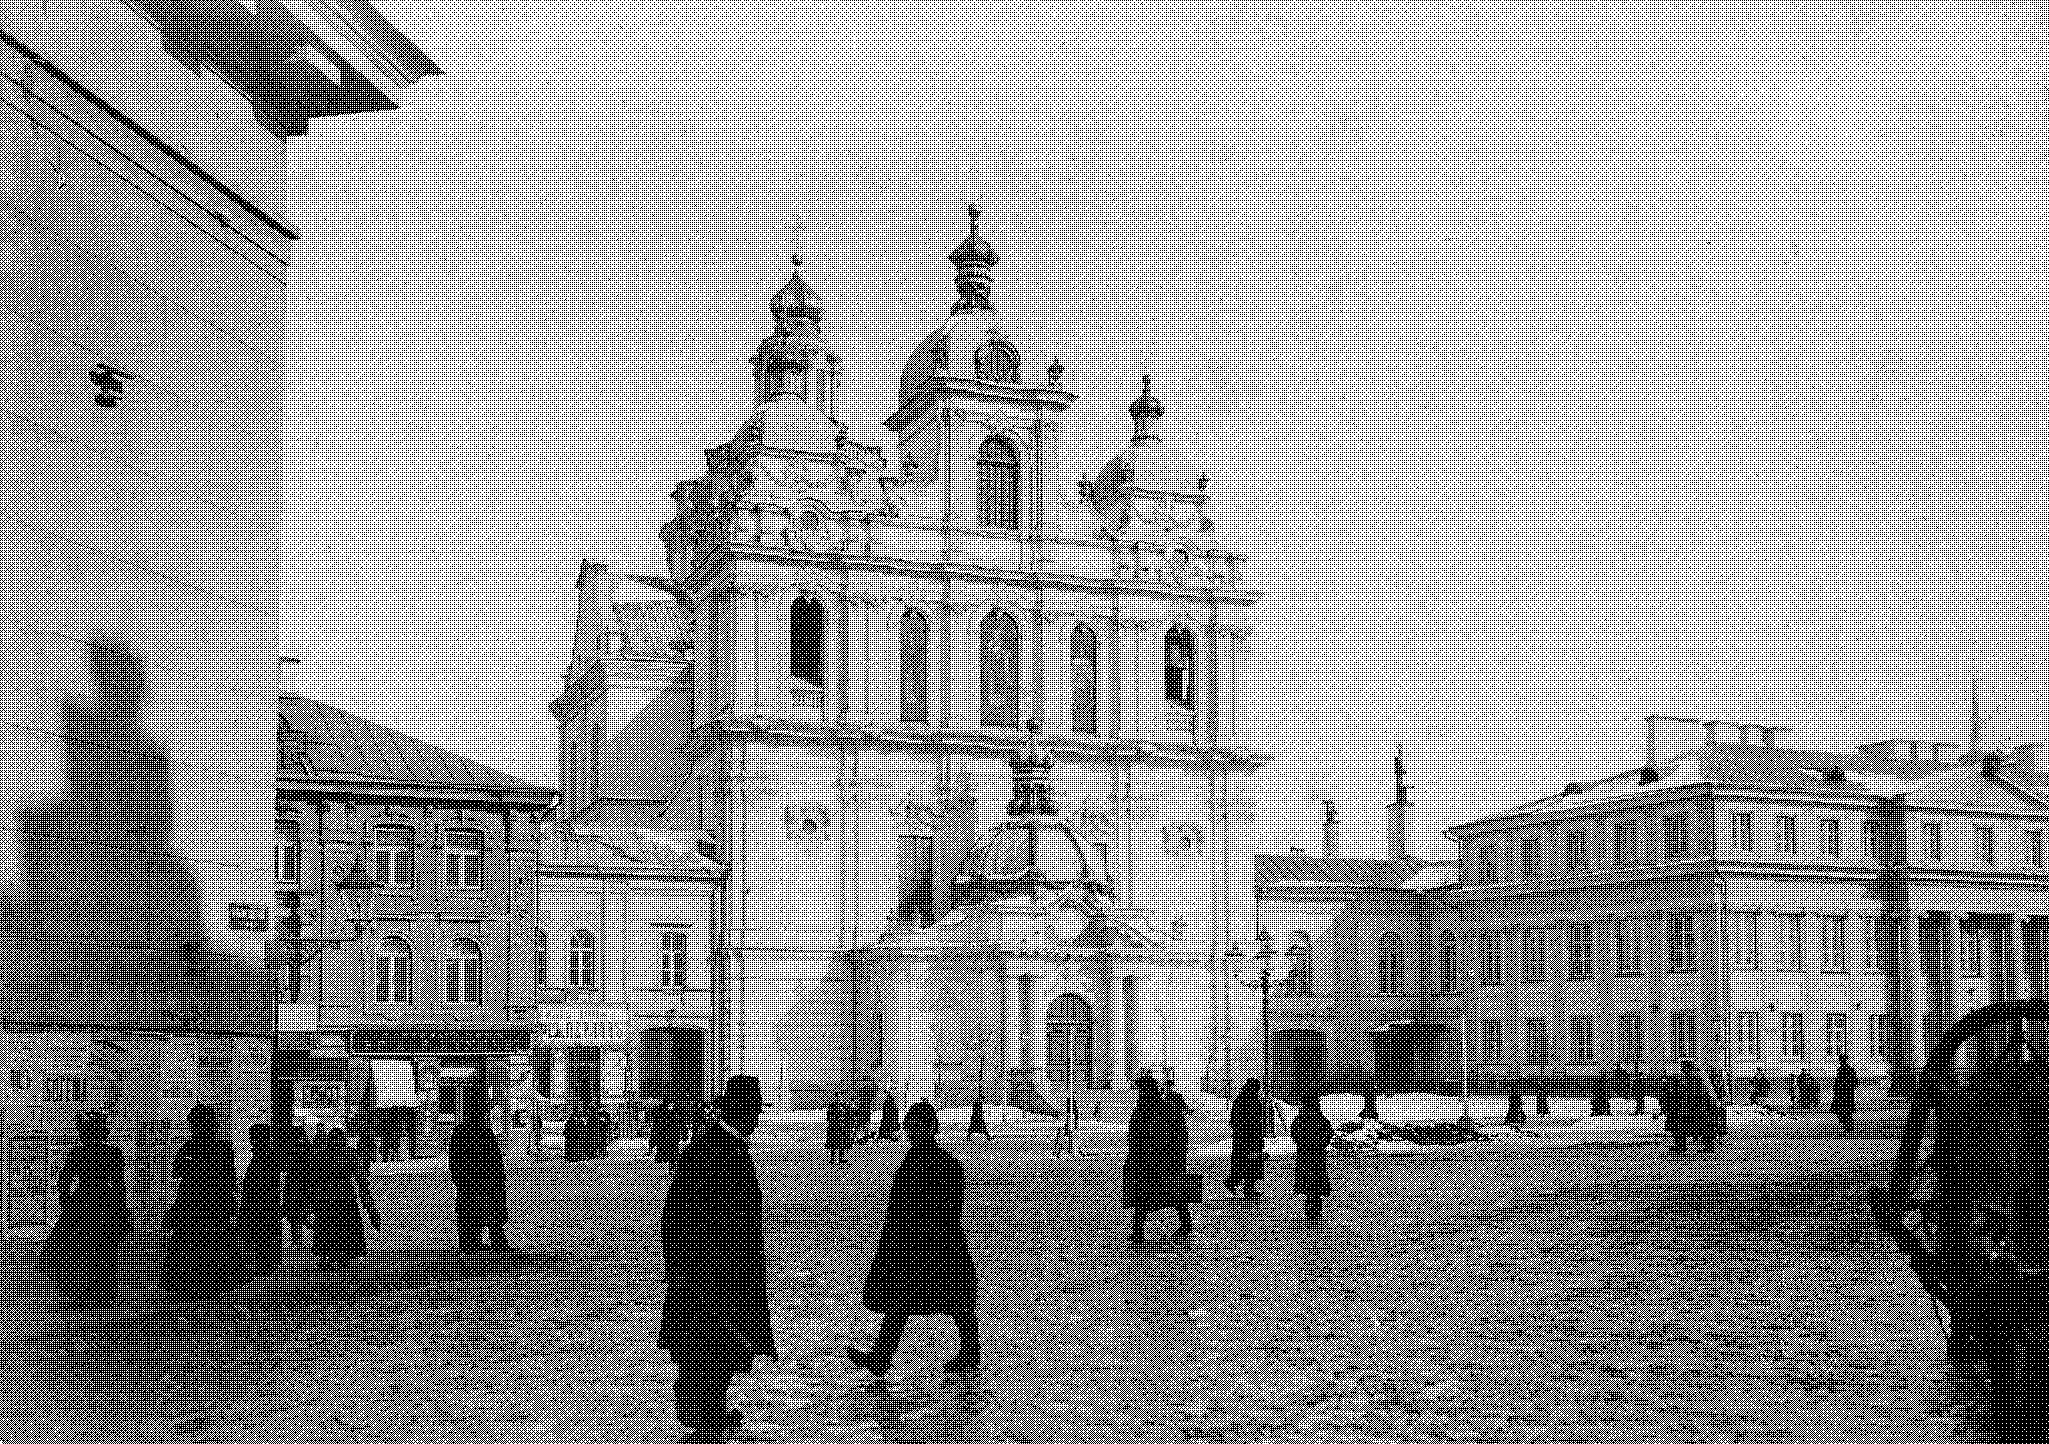
\includegraphics[width=10cm]{./ilustra-07.png} São Paulo\quad2021}
% \end{center}

\begin{figure}[!h]
    \centering
    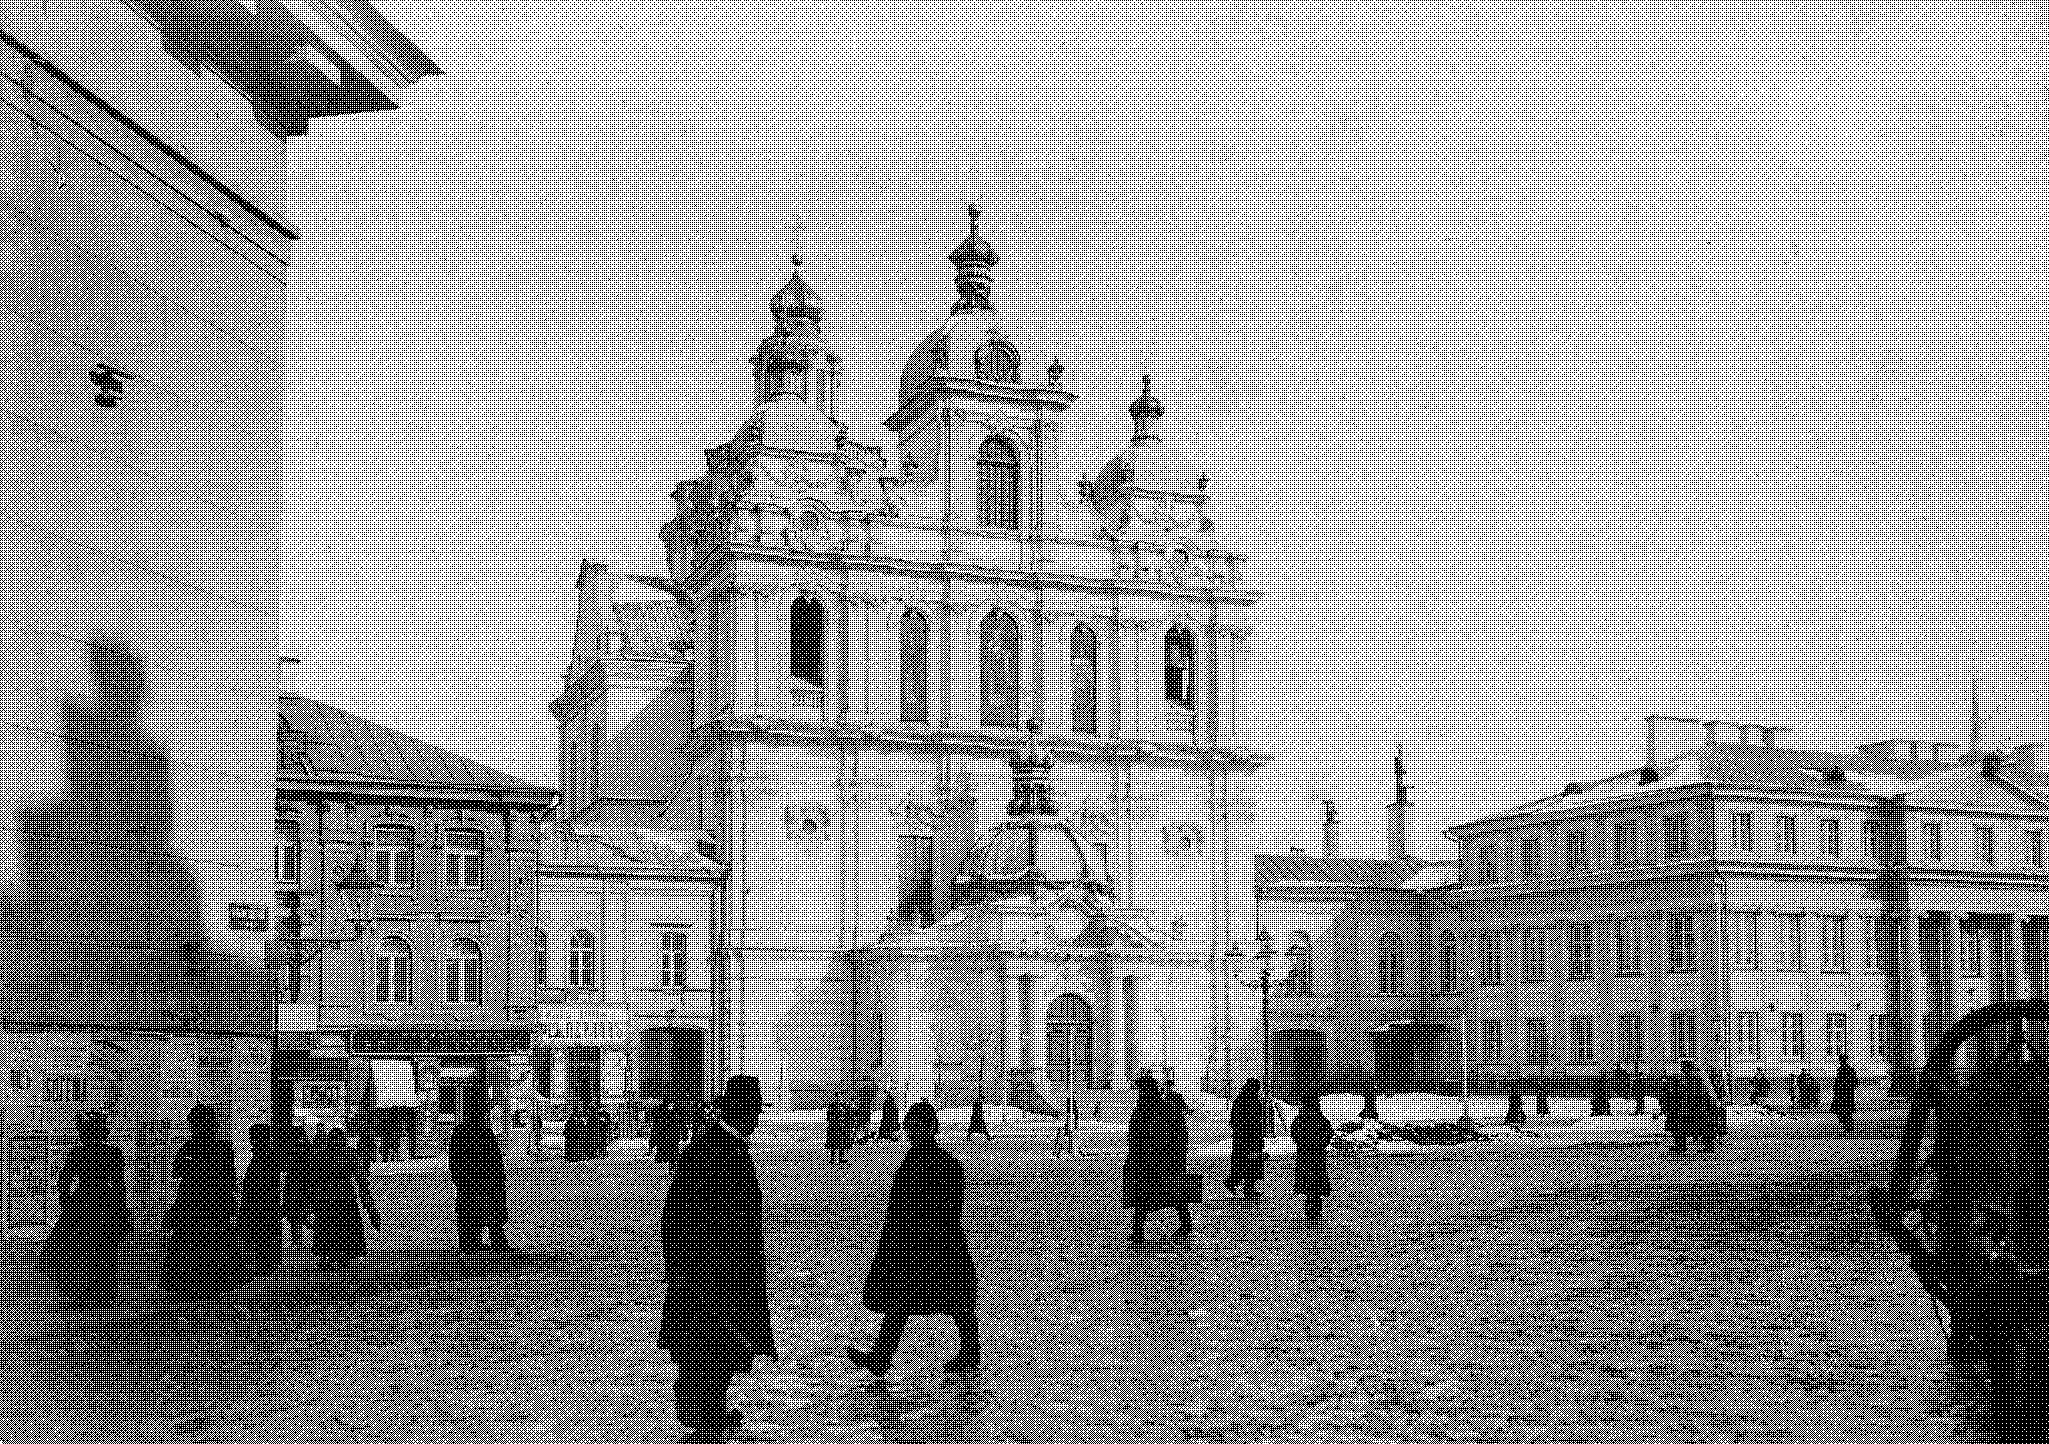
\includegraphics[width=\textwidth]{ilustra-07.png}
    \caption{A igreja católica de São Casimiro em Vilna foi interditada pelas autoridades tzaristas e, em 1840, readaptada para funcionar como a Catedral Ortodoxa Russa de São Nicolau. Fotografia tirada por volta de 1896.}
\end{figure}

O rápido sepultamento dos cadáveres foi supervisionado por colegas de
Frank, praticamente já no verão. Vilna parecia ter sido totalmente
limpa. Por sorte, não havia também sinais de epidemia. Segundo Frank,
isso teria sido motivado pela eficiência e habilidade das recém"-nomeadas
autoridades russas a cargo da prevenção de um surto. Mas foi útil também
o fato de a cidade estar apenas parcialmente habitada, pois muitos de
seus moradores retornaram muito lentamente. Apesar da guerra, havia
muita comida, e o tempo bom do verão prometia uma excelente colheita, de
modo que os preços dos produtos logo retornaram ao nível anterior à
guerra. Dentre todas as cidades da Lituânia visitadas pela família Frank
na viagem de volta para casa, Vilna parecia a que tinha menos sofrido.
De fato, o professor encontrou uma cidade em melhor estado do que antes
da guerra, graças ao novo governador russo, o enérgico General Korsakov,
que ``ordenou uma limpeza do estrume empilhado nos subúrbios, criou
novas avenidas, plantou árvores e repintou as casas manchadas e as
igrejas escoriadas.''\footnote{Ibid., p. 419.}

Na Vilna do pós"-guerra, a lealdade de Frank ao império russo o
comprometia aos olhos de muitos moradores. Embora uma anistia geral
houvesse sido concedida pelo tzar a todos os que serviram no exército
napoleônico ou no regime de ocupação, uma profunda desconfiança e
animosidade entre pró"-russos e pró"-franceses ainda dilacerava a cidade.
A universidade se tornou o epicentro da hostilidade: vários estudantes
haviam feito parte da \textit{Grande Armée} e, por conseguinte, morreram
durante a retirada. A vasta maioria do corpo docente também dera as
boas"-vindas a Napoleão como libertador da Lituânia. Apesar do apoio
sincero, a universidade não escapou ao saque. Durante a ocupação
francesa, seus prédios se transformaram em acampamentos e hospitais, e
praticamente todo o equipamento científico e inventário acadêmico foram
pilhados e destruídos. (Havia boatos a respeito de soldados famintos que
beberam e comeram todos os preparados anatômicos, mergulhados em álcool,
depositados na clínica da universidade.) As autoridades russas culparam
os membros colaboradores da faculdade pelo estrago. O velho reitor
Śniadecki foi obrigado a se exonerar, sugerindo"-se o leal Frank para
ocupar o cargo. Frank recusou a oferta, na esperança de preservar sua
neutralidade acadêmica e independência profissional.

Em meio a esse tumulto acadêmico, a família Frank, que recebeu uma
enxurrada de cartas implorando auxílio, procurava ajudar vários
refugiados e prisioneiros de guerra que permaneceram na cidade:

\begin{quote}
Nem todos sabiam que, durante a guerra, eu havia deixado Vilna. Meu pai
{[}em Viena{]} havia recebido inúmeras cartas de famílias francesas,
holandesas, alemãs e especialmente italianas implorando que eu mandasse
notícia de parentes por entre os prisioneiros de guerra na Rússia; em
caso de morte, pediram"-me que emitisse certidões de óbito, necessárias à
solução de questões de herança e outros problemas domésticos. Em Viena,
eu também havia recebido semelhantes pedidos. Com a ajuda de \textit{monsieur}
Horn {[}supervisor"-chefe dos prisioneiros de guerra na Lituânia{]}, fiz
o melhor que pude. Contudo, só fui capaz de obter informações de muito
poucos indivíduos. Em geral, as pessoas morriam sem ser contabilizadas
nos seguintes casos: muitos morreram congelados na estrada, queimados em
acampamentos militares ou afogados nos rios; alguns morreram de fome ao
lado de seus cavalos exaustos, por não terem tido energia de os
alimentar; e outros foram assassinados por camponeses russos e judeus
poloneses. `Você pode me dar informações daqueles que morreram nos
hospitais de Vilna,' perguntei a \textit{monsieur} Horn. ``Claro, mas só posso
fornecer informações daqueles que morreram após o restabelecimento da
ordem. Antes disso, não houve ocasião de registrar óbitos'' foi sua
resposta.\footnote{Ibid., p. 418.}
\end{quote}

Entre os sobreviventes da campanha, Frank encontrou o marido da irmã, o
Coronel Peternelli de Baden. Ademais, o professor encontrou também
colegas, conhecidos e mesmo antigos estudantes da Áustria, França,
Savoia, Tirol, Lombardia, Vestfália, Boêmia, Toscana e Nápoles. Sua
esposa também descobriu entre os refugiados um velho colega e amigo, o
famoso cantor lírico italiano Tarquini, que havia sido levado até Moscou
para divertir Napoleão.

A guerra também afetou enormemente a saúde da população local e, nesse
caso, Frank pôde ser decerto mais útil e eficiente. Ao chegar a Vilna,
pôs"-se imediatamente a investigar as trajetórias geográfica e social de
diversas enfermidades. Indicou a existência de uma correlação direta
entre o pico de transtornos cardiovasculares e o estresse causado pela
guerra. Pesquisou também uma condição psicológica hoje em dia conhecida
como transtorno de estresse pós"-traumático. Ao mesmo tempo, Frank
estimulou a pesquisa sobre a propagação da \textit{plica polonica}. Para
sua decepção, não encontrou nenhuma evidência da doença na Lituânia.
Após examinar alguns pacientes com sintomas atribuídos à \textit{plica
polonica}, ele chegou à conclusão de que a enfermidade, se é que
existisse, não era hereditária, contagiosa, ou causada pelo clima local.
Baseando"-se em observações científicas, ele determinou que a síndrome
era causada por nada mais que um remédio tradicional utilizado
equivocadamente no tratamento de diversos transtornos neurológicos. A
\textit{plica polonica} era uma moléstia causada pela má higiene a que
eram constrangidos, pela inércia médica da tradição, os pacientes
mentais. Ao que tudo indica, essa condição patológica, assim como a
própria Sarmácia, era mais invenção que realidade. Observadores
estrangeiros ignorantes, inclusive médicos, fizeram disso um mistério
cultural, transformando"-o numa sensação médica.

Frank acreditava também ser responsável por dissipar um pouco do
preconceito social local dirigido contra os sobreviventes da aniquilação
da \textit{Grande Armée}. Entre os centenas de refugiados civis da
retirada de Moscou que permaneceram em Vilna, havia uma certa Charlotte
Kops, nascida Devi, jovem intrigante, cuja origem nacional e estatuto
social foram encobertos por sua dramática estória de sobrevivência.
Conforme Frank, \textit{madame} Kops era uma inglesa elegante e bem educada que,
alguns anos antes de 1812, se casara com um comerciante polonês em
Moscou. Ninguém sabia por que \textit{madame} Kops chegara à Rússia, mas é
possível que lá houvesse inicialmente trabalhado como governanta.
Durante a ocupação francesa de Moscou, o comerciante foi nomeado
conselheiro municipal e o casal foi obrigado a fugir junto com a
\textit{Grande Armée}. Durante a retirada, \textit{madame} Kops alegou de maneira
ambígua ter protegido a si e a seu marido de morte certa. Os dois
chegaram sãos e salvos a Vilna mas, na colina Ponary, foram atacados
pelos cossacos e, no frio extremo, quase desnudos, viram"-se obrigados a
voltar à cidade. Apesar da colaboração do marido com os franceses, as
autoridades russas permitiram ao casal permanecer em Vilna, onde abriu
uma pequena forja. Charlotte Kops, devido a sua beleza e intrigante
estória de vida, foi de imediato percebida pelos espectadores da classe
alta e logo se tornou objeto de inúmeros boatos infames e aventuras
\textit{voyeuristas}. Era constantemente assediada por comentários de conotação
amorosa e sexual por parte dos homens, enquanto as mulheres da classe
alta lhe eram especialmente maldosas, pois, segundo Frank, repetidamente
``iam observá"-la em grupos ou utilizavam"-se de binóculos para analisar
seus traços. `Ela é muito bonita,' dizia uma. `Pena que suas maneiras
sejam tão inglesas,' respondia a outra.''\footnote{Ibid., p. 419.}

%{[}figura 38{]}
%
%A rua Ostrabrama, em Vilna, na primeira metade do século 19.

Intrigado e provavelmente seduzido por \textit{madame} Kops, Frank se tornou seu
padroeiro social e, possivelmente, amante. Ao invés, porém, de visitá"-la
em segredo na oficina, ele, num gesto dramático de afirmação pública,
era frequentemente visto na sua presença nos mais variados eventos. O
professor até mesmo a convidou até sua casa, onde a apresentou aos
membros da elite social de Vilna. Por um certo tempo, sua relação
ostensiva com \textit{madame} Kops escandalizou a cidade, mas talvez tenha sido
essa a reação que tentou provocar. Após seu retorno, Frank pareceu mais
assertivo em sua crítica à vida insular de Vilna. A ligação manifesta
com a Sra.\,Kops diferia em muito da relação anterior, mais discreta e
talvez mais afetuosa, com a Sra.\,Simpson, viúva do comerciante judeu.

Dez anos após ter retornado de Viena, Frank começou a contemplar deixar
Vilna. Embora se sentisse ligado à cidade e seus moradores, ele não
queria ter de escolher entre a lealdade ao regime tzarista e o
ressentimento local pelo mesmo. O compromisso de Frank para com Vilna
permaneceu vigoroso ao longo dos anos e, mesmo após a morte do filho
adotivo, Victor, em 1819, ele ainda nutria a esperança de adquirir uma
casa onde passar a vida de aposentado numa das áreas pitorescas da
cidade. Decidiu abandonar Vilna só no verão de 1823, quando a polícia
tzarista desvelou uma conspiração anti"-russa na universidade. O medo de
uma revolução ou revolta nacional (polono"-lituana) tomou conta da
administração imperial: o reitor da universidade foi detido e os
estudantes amotinados foram mandados para a prisão. Frank reconheceu
nessas prisões o fim da ``concórdia sarmácia''. Sabia que Vilna, sob o
domínio absolutista do império russo, haveria de se tornar um lugar
hostil e opressivo para se morar. Entretanto, ele evoca a decisão da
família de voltar a Viena como um dos mais dolorosos momentos de sua
vida:

\begin{quote}
Vou"-me lembrar sempre com carinho da gente de Vilna. O mais difícil foi
dizer adeus a meus pacientes, amigos e à cidade onde me encontrava tão
bem. Jamais me arrependi de ter passado os melhores anos da minha vida
neste país generoso. Certamente poderia ter obtido mais glória
profissional se tivesse lecionado num dos centros internacionais da
Europa, onde visitantes estrangeiros não são raros. Em Vilna, porém,
como em nenhum outro lugar da Europa, tive tantas oportunidades para
praticar meu conhecimento. Meu coração sangraria se os lituanos
pensassem que só vivi em Vilna por causa do dinheiro que eu poderia
gastar mais tarde alhures. Teria me aposentado com alegria na Lituânia, 
não tivesse eu experimentado ano passado uma tremenda angústia. Sabia
que, mais cedo ou mais tarde, uma tempestade varreria a
universidade.\footnote{Ibid., pp. 577--578.}
\end{quote}

%{[}figura 39{]}
%
%Mapa da ferrovia São Petersburgo --- Varsóvia, principal artéria de
%transporte entre a Rússia e a Europa Ocidental, 1863.

\chapter{A intriga russa}

%\setlength{\epigraphwidth}{.45\textwidth}
\begin{epigraphs} 
\qitem{Estou querendo ir à Europa, Aliócha, e partirei daqui; mas sei que vou
apenas visitar um cemitério, no entanto é o cemitério mais precioso,
mais precioso, é isso! Lá jazem os mortos, cada lousa sobre eles fala de
uma vida passada com ardor, de uma fé apaixonada em seus feitos, vou
cair por terra, beijar aquelas lousas e chorar sobre elas --- ao mesmo
tempo convencido de todo coração de que há muito tempo aquilo é um
cemitério e nada mais. E não vou chorar de desespero, mas pura e
simplesmente porque estarei feliz por minhas lágrimas derramadas. Vou
deleitar"-me com meu próprio enternecimento.}{\textit{Os irmãos Karamázov}, \textsc{fiódor dostoiévski}\footnotemark}
\end{epigraphs}

\footnotetext{Conforme tradução feita por Paulo Bezerra de \textit{Os irmãos Karamázov}, São Paulo: Editora 34, 2008, p. 318. [\textsc{n.\,t.}]}

As guerras napoleônicas transformaram a Europa em benefício da Rússia
tzarista. Depois que o exército russo chegou a Paris, varrendo o
continente atrás dos restos da \textit{Grande Armée}, o país adentrou em
cheio na era imperial. 
O Congresso de Viena, reunido em 1814 pelas
potências vitoriosas, selou o destino de Vilna --- a cidade, junto com
a maior parte do território do antigo Grão"-Ducado, haveria de ficar com a
Rússia. Embora a Rússia imperial houvesse absorvido a Lituânia nos
últimos anos do século \textsc{xviii}, foi só durante as sufocantes décadas do
governo de Nicolau \versal{i} (o inflexível irmão menor de Alexandre \versal{i}, que subiu
em 1825 ao poder pela repressão de um motim liberal militar) que o
regime imperial restritivo chegou a ser sentido em sua totalidade.
Inevitavelmente, a Guerra de 1812, batizada na Rússia como Grande Guerra
Patriótica, se transformou num ponto essencial de referência da
autoridade russa sobre Vilna. Estimulada pelos vizinhos europeus, a
família tzarista governou Vilna valendo"-se do direito divino
pré"-concebido, suposta prerrogativa de todo império. No entanto, aos
olhos da sociedade russa como um todo, poloneses e lituanos, com suas
lealdades oscilantes e teimosia paroquial, jamais seriam confiáveis. O
sonho da nobreza local de ressurreição de sua República fracassada era
considerado importante fonte de instabilidade na Europa. Nessa concepção
geopolítica, a Rússia era apoiada pela Prússia e Áustria; França e
Inglaterra, por outro lado, nutriam mais simpatia pela causa
polono"-lituana. Contudo, no mapa geopolítico mais amplo da Europa, o
controle russo sobre a Lituânia contribuiu para o equilíbrio de poder no
continente por quase um século. Para a Rússia, Vilna era o guardião da
fronteira imperial com a Europa Ocidental. A cidade era considerada lar
russo de direito, mesmo que corrompido pela desordem e espírito
insubmisso.

Meio século se passara entre a era das guerras napoleônicas e a
publicação de \textit{Guerra e paz}, de Liev Tolstói. O Conde Tolstói
(1828--1910), que passou mais de uma década escrevendo o romance, examina
aquele período histórico a partir da perspectiva da sociedade russa e,
entre muitas outras coisas, \textit{Guerra e paz} trata do lugar da Rússia
na Europa. Nesse retrato intimamente panorâmico da vida durante a
guerra, Vilna se torna ponto importante de transição geopolítica. É o
local onde a Mãe Rússia se transforma em império, permutando assim o
ideal heroico de auto"-sacrifício nacional pela arrogância de um
conquistador imperial. Para Tolstói, cruzar Vilna era como um rito de
honra: a leste da cidade ficava a Rússia --- terra familiar que oferece
conforto espiritual e respeito de si; a oeste --- a Europa --- território
estrangeiro que põe em dúvida o caráter nacional e incita ao
constrangimento.

Na primavera de 1861, Tolstói fez uma breve parada em Vilna em sua
viagem de trem de Berlim até São Petersburgo. O escritor de quarenta e
um anos atravessou a fronteira entre a Prússia e a Rússia em 12/24 de
abril (conforme os calendários juliano e gregoriano). Resumiu assim o
dia em seu diário: ``Fronteira. Mal se nota a sã e feliz Rússia.'' A
anotação feita em 13/25 de abril --- muito provavelmente o dia da visita a
Vilna --- é mais impenetrável. ``Noite com os judeus. Lehman, ambiente
alegre. Frio na carruagem, o vendedor tomou emprestado um pouco de
dinheiro\ldots{}''\footnote{Liev Tolstói, conforme citado em Birutė Masionienė, \textit{Levas Tolstojus ir Lietuva}. Vilna: Vaga, 1978, pp. 11--12.} Tolstói criou em seu romance uma imagem mais extensa e memorável de Vilna. No início, a cidade surge brevemente por ocasião da
chegada da \textit{Grande Armée} ao território russo. Um relato mais
minucioso, porém, desponta no fim do romance, com o retrato final de
Kutuzov, comandante russo vitorioso:

\begin{quote}
No dia 29 de novembro, Kutúzov entrou em Vilna --- sua boa Vilna, como ele
dizia. Duas vezes em seu tempo de serviço, Kutúzov fora governador de
Vilna. Na rica Vilna, que havia sobrevivido à guerra, além dos confortos
da vida dos quais ele estava privado havia tanto tempo, Kutúzov
encontrou velhos amigos e recordações. E ele, de repente pondo de lado
todas as preocupações militares e de governo, mergulhou numa vida
sossegada, rotineira, ao menos na medida em que as paixões que ardiam à
sua volta lhe davam repouso, como se tudo o que acontecia agora, e o que
tinha de acontecer no mundo histórico, não lhe dissesse o menor
respeito.

[\ldots{}] No dia seguinte houve um jantar na casa do marechal de campo e
também um baile que o soberano honrou com sua presença. A Ordem de São
Jorge de primeira classe tinha sido concedida a Kutúzov; o soberano lhe
conferia a mais alta distinção; mas a insatisfação do soberano com o
marechal de campo era conhecida de todos.

[\ldots{}] A insatisfação do soberano com Kutúzov aumentou em Vilna sobretudo
porque Kutúzov obviamente não queria ou não conseguia entender a
importância da campanha futura.

Quando, no dia seguinte pela manhã, o soberano disse para os oficiais
reunidos à sua volta: ``Os senhores salvaram não só a Rússia; salvaram a
Europa'', todos já haviam entendido que a guerra não havia terminado.

Só Kutúzov não queria entender aquilo e manifestava abertamente sua
opinião de que uma nova guerra não poderia melhorar a situação e
aumentar a glória da Rússia, mas poderia apenas piorar a situação e
rebaixar a glória suprema que, a seu ver, a Rússia então havia
alcançado. Tentou mostrar ao soberano a impossibilidade de convocar
tropas novas; falou da situação penosa da população, da possibilidade de
um fracasso etc.

[\ldots{}] A guerra de 1812, além de seu significado, caro ao coração do povo
russo, deveria ter outro significado --- europeu.

Após o movimento dos povos do Ocidente para o Oriente, deveria se seguir
outro, do Oriente para o Ocidente, e para aquela nova guerra era
necessário um ator novo, com características e opiniões diferentes de
Kutúzov e guiado por outras motivações.

Para o movimento dos povos do Oriente para o Ocidente e para a
restauração das fronteiras nacionais, Alexandre \versal{i} era tão necessário
quanto tinha sido Kutúzov para a salvação e a glória da Rússia.

Kutúzov não entendia o que significava a Europa, o equilíbrio, Napoleão.
Não conseguia compreender isso. Para o representante do povo russo,
depois que o inimigo fora aniquilado, a Rússia estava liberta e se
alçara à sua glória suprema; para um russo, enquanto russo, não tinha
sentido fazer ainda algo mais. Para o representante da guerra popular,
não restava outra coisa senão a morte. E ele morreu.\footnote{Conforme tradução feita por Rubens Figueiredo de \textit{Guerra e paz}, São Paulo: Cosac Naify, 2011. [\textsc{n.\,t.}]} 
\end{quote}

Enquanto Vilna, na obra ficcional de Tolstói, se apresenta como uma
reconfortante cidade russa, o jugo tzarista sobre ela e a Lituânia
inteira, na realidade, não foi nada sereno. Os cento e vinte anos de
dominação russa (1795--1915) foram pontuados por três guerras de
insurreição --- 1812, 1830--1831 e 1863--1864 --- e a revolução de 1905. Cada
um desses conflitos alterou a natureza política do regime imperial,
assim como a hierarquia sócio"-cultural local.

O período anterior à insurreição de 1830--31 foi marcado por uma relativa
tolerância para com as atividades culturais e religiosas polonesas e
também, até um certo limite, lituanas. No geral, muitos costumes e
instituições tradicionais da Lituânia, tais como o código legal, certos
privilégios provinciais da nobreza, e a preponderância da igreja
católica, foram mantidos. A perseguição e censura políticas em Vilna só
aumentaram depois da descoberta, em 1823, de uma conspiração
revolucionária na universidade entre os estudantes poloneses. Em geral,
a Universidade Imperial havia formado uma nova geração de
administradores e especialistas, tais como médicos, geógrafos e
geólogos, para todo o império russo. Contudo, em especial depois de
1812, a universidade se tornou o centro nervoso da resistência
intelectual polonesa contra a dominação tzarista na região. Seus mais
famosos estudantes foram os poetas românticos poloneses Adam Mickiewicz
e Juliusz Słowacki.

A universidade foi fechada em 1832 por decreto de Nicolau \versal{i} após a
supressão da insurreição polono"-lituana. No lugar, as autoridades
tzaristas abriram a Academia Médica, que também foi dissolvida em 1842,
e o Seminário Católico, que em 1844 foi transferido para São
Petersburgo. A maior parte dos recursos institucionais da universidade ---
professores, biblioteca e arquivos --- foi transferida para outras
academias russas. Essas e muitas outras repressões educacionais e
culturais diminuíram o estatuto intelectual de Vilna: após mais de dois
séculos e meio de vida universitária ativa, Vilna deixava de ser uma
importante cidade acadêmica.

Ambos os lados --- russos e poloneses --- viam a Lituânia como província
ocupada. Os russos procuravam suprimir a polonização cultural e
linguística da região, enquanto os poloneses resistiam à crescente
russificação. Após a escandalosa erradicação das organizações
patrióticas estudantis em Vilna, a administração russa impôs também um
novo currículo educacional às escolas primárias na Lituânia. A fim de
realinhar a região à visão de mundo do império, decidiu"-se pelo ensino
de história e geografia exclusivamente em língua russa, ao invés do
habitual polonês. A iniciativa pretendia contrabalançar a influência
cultural da igreja católica e da nobreza local de fala polonesa, mas
pouco fez para criar uma nova geração de súditos russos leais.

No núcleo da batalha cultural estavam as lealdades religiosas da
população. A administração e \textit{intelligentsia} russas com frequência
equiparavam o patriotismo polonês ao fanatismo conspiratório jesuíta,
criando uma imagem de conflito russo"-polonês como uma batalha entre o
racionalismo moderno e a irracionalidade medieval. Depois de 1831, o
regime tzarista deu início a uma ampla campanha anti"-católica: o
patrimônio da igreja foi expropriado e os mosteiros, fechados. Contudo,
a principal vítima da repressão religiosa tzarista na Lituânia foi a
igreja greco"-católica. Em 1839, a prática da fé greco"-católica foi
proibida e seus poucos milhões de seguidores foram forçados a integrar a
igreja ortodoxa russa. Em Vilna, essa assimilação religiosa forçada
pouco influenciou no enfrentamento da supremacia demográfica católica. A
fim de reduzir a visibilidade católica na cidade, as autoridades
tzaristas converteram diversas igrejas em templos ortodoxos. A igreja de
São Casimiro foi transformada na basílica de São Nicolau, sua fachada
romano"-barroca ganhando características distintivamente ortodoxas
russas.

%{[}figura 40{]}
%
%A igreja católica de São Casimiro em Vilna, no aspecto assumido após a
%insurreição polono"-lituana de 1863--1864 contra o domínio tzarista,
%quando foi transformada na catedral ortodoxa russa de São Nicolau.

A russificação e a subsequente modernização de Vilna afetou os judeus
locais de uma maneira diferente. Antes da anexação da Polônia"-Lituânia
no fim do século \textsc{xviii}, havia muito poucos judeus na Rússia. Na virada do
século \textsc{xx}, havia mais de quatro milhões e meio de judeus morando no
império russo, quase dois terços de todos os judeus da Europa. Com cerca
de setecentos mil judeus vivendo nas províncias lituanas, a região
detinha uma das maiores concentrações de população judaica (cerca de
quinze por cento do total) na Europa. A administração tzarista sempre
tratou essa numerosa população judaica com grande suspeita e,
imediatamente após a incorporação das terras anexadas, implantou
restrições à migração judaica para outras partes do império. A Zona de
Assentamento Judeu coincidia aproximadamente com o território histórico
da República Polono"-Lituana. Em várias ocasiões, as autoridades
tzaristas procuraram também eliminar a autonomia comunitária e as
distinções culturais dos judeus. Em 1844, \textit{Kahal}, o mais antigo órgão
de auto"-determinação da comunidade judaica, foi abolido. Escolas
russófonas para crianças judias foram instituídas por toda a Zona, e
dois seminários rabínicos estatais, um deles em Vilna, foram
estabelecidos. Em 1851, homens judeus foram proibidos de usar roupas
tradicionais e cachos laterais, \textit{peiot}, e mulheres judias foram
obrigadas a parar de raspar a cabeça. A maioria dessas iniciativas
punitivas jamais entrou em vigor, limitando a assimilação judaica. Por
outro lado, a grande concentração de judeus na Zona contribuiu para um
incomparável florescimento da vida judaica sob os aspectos cultural,
social e religioso. Por conseguinte, a Zona se tornou o centro do
judaísmo \textit{ashkenazi}, onde amadureceram importantes desdobramentos da
história judaica moderna --- hassidismo, sionismo e cultura iídiche.

%{[}figura 41{]}
%
%Entrada do pátio da Velha Sinagoga de Vilne, cerca de 1900.

Entre os judeus, \textit{Vilne} ficou conhecida como \textit{Yerushalaim
d'Lita}.\footnote{Em português, ``Jerusalém da Lituânia''.} Segundo a lenda, Napoleão foi o
primeiro a dar a \textit{Vilne} o nome de Jerusalém. Dizem que a força numérica e
a religiosidade da comunidade judaica local lembrou o imperador francês
da Jerusalém na Terra Santa, onde havia estado durante a fracassada
campanha egípcia de 1798--1799. Para a maior parte dos judeus,
entretanto, o título de \textit{Yerushalaim d'Lita} era menos associado a
Napoleão que à vigorosa cultura judaica que ali se desenvolveu. Em
primeiro lugar, \textit{Vilne} ganhou o título de Jerusalém do Norte devido à
renomada erudição de Eliyahu ben Shlomo Zalman (1720--1797), mais
conhecido como o Gaon de \textit{Vilne}, cuja vida e obra materializaram o ideal
da existência judaica no exílio. Na virada do século \textsc{xx}, \textit{Vilne} se
tornara o lugar onde, nas palavras de Benjamin Harshav, ocorreu a
revolução judaica moderna:

\begin{quote}
O apelido ``Jerusalém da Lituânia'' se baseou na solidez do ensino
judaico e da impressão de todo o Talmude babilônico em Vilna. Parece,
contudo, que foi o movimento secular, que em Vilna foi percebido como
herdeiro da tradição religiosa, que inventou e promoveu aquele nome. Em
1859, publicou"-se um livro em hebraico de autoria do \textit{maskil}\footnote{Escritor
iluminista, seguidor do movimento judaico da \textit{Haskalá}.} e erudito Rashi Fin (Samuel Joseph Fuenn), que descrevia a
história de Vilna e sua comunidade judaica. O livro se chamava \textit{Kiryá
ne'emaná}, ou ``Cidade piedosa'', e descrevia Vilna nos termos bíblicos em
geral utilizados para Jerusalém. Se já existisse o nome ``Jerusalém da
Lituânia'', Fin o teria usado. Mas é o oposto: foi a partir do nome do
livro que o apelido se originou. Os movimentos iídiche e secular de
Vilna, assim como a poesia moderna hebraica, adotaram o nome, orgulhosos
de dar seguimento à tradição do Gaon de Vilna.

[\ldots{}] À semelhança de Jena e Weimar, Cambridge e Oxford, Vilna era
uma cidade pequena, um centro cultural que servia a uma extensa
província. Os laços dentre Vilna e a rede de cidadezinhas eram muito
estreitos, as pessoas iam e vinham, a cidade servia como uma espécie de
`shopping center' e centro cultural para toda a região, e várias
pequenas cidades desempenhavam também importantes papéis: \textit{yeshivás}
famosas podiam ser encontradas em cidadezinhas tais como Volozhin, Mir,
Ponevezh; uma grande seita hassídica, Chabad, que surgiu na Lituânia
oriental, tinha sua capital em Lubavitch, uma cidade de 1667 judeus. De
fato, a maioria dos escritores e intelectuais de Vilna nasceram
alhures\ldots{} Por outro lado, inúmeros jovens de cidades menores se
mudaram para a capital a fim de estudar no Seminário Rabínico ou nas
Faculdades de Educação Hebraica ou Iídiche, para então retornar a suas
pequenas cidades ou emigrar para a Palestina ou para o Ocidente.

Portanto, quando uma cidade de meros 60 mil judeus percebeu ser um
importante centro de uma cultura que se espalhara pelo mundo, isso se
deveu a suas instituições culturais e aos milhões de judeus do Leste
europeu que a serviam e representavam.\footnote{Prefácio de Benjamin Harshav em Herman Kruk, \textit{The Last Days of the Jerusalem of Lithuania: Chronicles from the Vilna Ghetto and the Camps, 1939--1944}, trad. Barbara Harshav. New Haven: Yale University Press, 2002.} 
\end{quote}

Para a comunidade católica local, o nome de Jerusalém tinha um
significado diferente. Na década de 1660, em agradecimento pela
libertação da Lituânia da ocupação russa, o bispo católico local criou
uma trilha da Via Dolorosa numa encosta suave e cheia de árvores do rio
Neris, ao norte da cidade. A réplica barroca do Calvário se tornou um
importante local de peregrinação na Lituânia, e deixou sua marca na
toponímia local: um riacho próximo foi renomeado Cédron e o vilarejo
vizinho ganhou o nome de Jerusalém, nome utilizado até os dias de hoje.

Os russos, que jamais foram mais que um quinto da população local,
sentiam"-se ameaçados pela forte presença católica e judaica naquele
lugar. Durante todo o período do governo imperial, a população de Vilna
se manteve em constante fluxo. Enquanto muitas pessoas se mudavam para a
cidade vindo das províncias adjacentes, um grande número a deixava rumo
a centros metropolitanos mais prósperos ao redor do mundo. A população
russa, que consistia sobretudo em oficiais militares e administrativos
com as respectivas famílias, era ainda mais instável. Mais efêmeros
ainda eram os governadores russos de Vilna: nos cento e vinte anos de
administração tzarista, eles totalizaram quase trinta.

Mas nem todos os russos, nem todos os residentes ortodoxos da cidade
eram colonos. Os laços culturais e religiosos entre Vilna e Bizâncio
(ou, nesse caso, Moscóvia) existiam desde os primórdios históricos da
cidade. Várias esposas de grão"-duques lituanos católicos e pagãos, por
exemplo, vinham de famílias de príncipes russos. E os primeiros mártires
cristãos locais eram de fé ortodoxa bizantina. Essa conexão próxima e
quase sempre íntima entre Vilna e a cristandade oriental fez da
colonização imperial russa um processo mais imaginativo, porém não menos
brutal. No fundo, muitos russos se sentiam na cidade como seu lar de
direito, mesmo que a vivenciassem só como um lugar de passagem.

Com a crescente repressão política e o fechamento da universidade, o
estatuto de Vilna no império russo, como uma das maiores e uma das mais
vibrantes cidades do ponto de vista intelectual, foi aos poucos
esmorecendo. Depois de 1812, imperadores e dignitários russos raramente
visitaram a cidade. Perto do fim do governo tzarista, Vilna era uma
cidade provinciana de tamanho médio, com pouca riqueza financeira ou
potencial industrial. O que salvou a cidade da ruína econômica e
esquecimento foi a ferrovia. O primeiro trem chegou de Dvinsk
(Daugavpils em letão, ou Dunaburg em alemão) vindo da direção da capital
imperial de São Petersburgo em 4 de setembro de 1860. No ano seguinte, a
inauguração de uma linha férrea até a fronteira russo"-prussiana passou a
conectar a cidade a Königsberg e Berlim.\footnote{J. Jurginis, \textsc{v}.\,Merkys e \textsc{a}.\,Tautavičius, op. cit., pp. 275--276.} Finalmente, com a conclusão da linha São Petersburgo --- Varsóvia em 1862, Vilna foi
definitivamente pregada ao mapa do império como importante eixo de
transporte.

\asterisc

Ao viajar de Berlim a São Petersburgo na última década do século \textsc{xix}, o
etnógrafo dinamarquês Age Meyer Benedictsen (1866--1927) descreveu o
trajeto pela Lituânia numa série de instantâneos aleatórios:

%{[}figura 42{]}
%
%Mapa de Vilna, 1882.

\begin{quote}
Muita gente passou pela Lituânia sem conhecê"-la ou sem se importar com
ela. As grandes linhas férreas que conectam as capitais da Rússia e
Alemanha atravessam justamente o território de Gediminas, atravessam
justamente a terra em que ainda moram camponeses lituanos. Sentados em
vagões confortáveis, homens e mulheres contemplam com indiferença a
paisagem de certo modo monótona com seus vastos acres de milharais
ondulantes, com seus meândricos bosques de bétulas e bordos, carvalhos e
abetos. Passamos com velocidade diante de casarões baixos de madeira, e
o trem para em estações com nomes peculiares, Schillen, Pilkallen,
Gumbinnen, Eydtkuhnen, nomes que se querem alemães mas que soam tão
estrangeiros; mas são só esses nomes que interferem com a ideia de
estarmos viajando pela Alemanha. Tudo no trem é alemão, os passageiros,
os guardas, os avisos impressos; as estações ferroviárias se parecem com
as da Rheinland e Hannover, com o mesmo ``Vorstand'' de quepe vermelho,
a mesma afetação de ombros das garçonetes, os mesmos garçons nos mesmos
salões de estilo \textit{altdeutsch}. Ao chegarmos à fronteira, vemos pela
última vez a bandeira preta, branca e vermelha, o capacete pontudo e a
organização alemã --- atravessamos a linha e estamos na Rússia. Devemos
apresentar os passaportes, e vemos cartazes naquelas letras angulares
que nos incomodam por não entendê"-las. Policiais em azul escuro e galões
vermelhos caminham pela plataforma deserta. Então chegam os oficiais da
alfândega, vagões são trocados, vacas russas são embarcadas e ouvimos a
língua russa, assim como era de se esperar em chegando à Rússia --- e o
trem continua a todo vapor. De novo estações que para um neófito
poderiam ter nomes russos, mas que aos próprios russos soam
estrangeiros: Gielgudiski, Vilkoviski, Pilviski e assim por diante. Nos
vagões, ouve"-se russo, alemão e talvez também polonês. Policiais e
soldados de blusas pretas com bonés redondos, sinos, botas de cano longo
e capas cinza jogadas à vontade por sobre os ombros podem ser vistos em
cada estação, e também um tipo muito peculiar, novo para nós,
ocidentais, o célebre judeu polonês, com sua figura desagregada vestindo
roupas surradas, de mãos dobradas e barba despenteada, uma massa de
feiura que, à primeira vista, parece tudo explicar --- seu caráter, sua
maneira de viver e sua existência de pária. Passaram"-se metade de um dia
e metade de uma noite em que ou dormimos ou contemplamos preguiçosamente
a paisagem plana, escutando o estrondo das rodas pelas pontes sobre os
rios, ou chacoalhando entre os pinheirais. Teria sido possível observar,
com certo interesse, um grupo de cossacos pernaltas com quepes achatados
e pescoços grossos, que haviam saído montados em seus cavalinhos feios
junto à ferrovia, eles tanto se parecem com aquilo que se escreve sobre
eles, que é impossível não achar um pouco engraçado. Teria sido possível
também observar carruagens de madeira desajeitadas, atreladas a três
cavalos gordos que vigorosamente pisam no chão e bufam em resposta às
palavras do cocheiro; haviam vindo do casarão vizinho a fim de encontrar
o escudeiro na volta de sua viagem ao Exterior. Aqui e ali, abóbadas em
forma de cebola, douradas ou verdes, passam rapidamente e chega"-se enfim
a uma cidade grande, Dunaburg, após atravessar toda a Lituânia sem se
tornar, diga"-se de passagem, mais sábio por causa disso.\footnote{Age Meyer Benedictsen, \textit{Lithuania, The Awakening of a Nation -- a Study of the Past and Present of the Lithuanian People}. Copenhagen: Egmont \textsc{h}.\,Petersens, 1924, pp. 139--141.} 
\end{quote}

Enquanto tornava a Lituânia mais misteriosa, a ferrovia também trazia
muitos visitantes ocasionais até Vilna. Nos estágios iniciais da viagem,
todos os passageiros indo da ou para a Rússia eram obrigados a
desembarcar e baldear em Vilna. A parada obrigatória marcava o nome da
cidade no itinerário de todos. Mas chegar de trem escondia a visão que
se costumava ter ao se aproximar da cidade: o túnel ferroviário mais
comprido do império, inaugurado em 1860 pelo Tzar Alexandre \versal{ii}, cortava
a colina Paneriai, também conhecida como Ponary. Durante séculos, quem quer que chegasse à
cidade podia se maravilhar com sua posição panorâmica, mas o túnel
escuro de parapeito íngreme --- maravilha da engenharia do século \textsc{xix} --- não
dava tempo nem permitia a sua visão. Após alguns minutos de escuridão, o
trem chegava a uma estação ferroviária ordinária, construída na
periferia da cidade. Era um prelúdio miserável para Vilna.

A partir de meados do século \textsc{xix}, tornou"-se possível e estava na moda,
para os intelectuais russos, viajar à Europa. Uma viagem de lazer para o
Exterior era uma questão sazonal: ela em geral coincidia com o início do
verão nos famosos spas da Europa Ocidental ou com as férias de inverno
na costa do Mediterrâneo. Muitos daqueles que viajavam, como Tolstói,
escreviam anotações ou diários, em que Vilna marcava o início ou o
término da aventura europeia. Nesse contexto, a cidade se tornara um
portão de acesso, na experiência tanto do real como das narrativas.

O dramaturgo russo Aleksandr Ostrovsky (1823--1886) visitou Vilna na
primavera de 1862. As peças de Ostrovsky revelavam as degradantes
condições sociais do sistema capitalista russo emergente, não raro a
partir da perspectiva da difícil situação das mulheres. Nicolau \versal{i} em
pessoa mandou censurar sua obra e o colocar sob vigilância policial mas,
durante os anos liberais de Alexandre \versal{ii}, foi"-lhe permitida mais
liberdade criativa e pessoal. O realismo social de suas peças era do
agrado do público: sua obra era tão popular que até mesmo o guia de
língua inglesa Murray recomendava àqueles que visitassem Moscou e
``talvez não compreendam os diálogos'' que fossem assistir a suas peças
a fim de ``estudar o comportamento e os costumes do país assim como se
apresentam no palco.''\footnote{\textit{Handbook for Travellers in Russia, Poland and Finland}. Londres: John Murray, 1867, p. 173.}

Antes da viagem à Europa, o dramaturgo, que contava então 39 anos, se
propôs a escrever um diário. Em contraste com Tolstói (que só foi capaz
de voltar para casa pela recém"-inaugurada ferrovia), Ostrovsky saiu da
Rússia de trem. A primeira anotação foi redigida em Vilna:

\begin{flushright}
\smallskip\hfill\textsc{2 de abril}
\end{flushright}
\smallskip
\begin{quote}
Deixamos Petersburgo em 2 de abril (segunda"-feira) às 3 da tarde.
[\ldots{}] Decidimos ficar em Vilna e visitar as atrações locais.
\end{quote}

\begin{flushright}
\smallskip\hfill\textsc{3 de abril}
\end{flushright}
\smallskip
\begin{quote}
Ao meio"-dia e meia chegamos em Vilna. O tempo está esplêndido, nenhum
sinal de neve; em Moscou, um tempo assim só temos no fim de abril.
Ficamos no hotel Jmurkevich, atrás do portão Ostra Brama. À primeira
vista, a cidade surpreende com sua originalidade. Ela é toda construída
de pedra, com ruas estreitas e inacreditavelmente limpas, casas altas
cobertas de telhas e igrejas majestosas para onde quer que se olhe.
Almoçamos no Yodke; é uma pequena taverna --- apenas duas salas --- em que
trabalham um jovem rapaz, a filha do dono e o próprio dono, que é ator e
está sempre com um copo de vinho Madeira na mão. Após o almoço, fomos
visitar a cidade. Por sobre ela vela uma serra com inúmeros picos
cônicos; em cima de um deles há uma torre. Essas colinas e a cidade
apresentam uma visão invulgar e incrivelmente bela. Alugamos um coche
para subir a serra; passamos em frente à igreja de São João, à casa do
governador, à Catedral (entramos), e chegamos às margens do rio Viliya,
que estava inundado; perto da caserna, deixamos o coche e começamos a
subir a encosta íngreme da colina. Queríamos muito ver a cidade de cima
e, lá pelas quatro da tarde, bem dispostos, chegamos de certa forma ao
topo da montanha: ao que parece, o lugar era protegido por militares
que, brutais, nos deram ordem de descer imediatamente. Em nossa
caminhada para baixo, um amável estudante do ginásio local havia reunido
as primeiras flores da primavera (anêmonas). Ele as ofereceu a nós. As
flores aqui já florescem, enquanto a grama fresca começa a brotar.
Voltamos ao nosso coche e decidimos visitar a igreja de São Pedro e São
Paulo. À esquerda, temos o rio Viliya e, à direita, colinas cobertas por
pinheiros: lugar perfeito para se divertir no verão. A igreja do lado de
fora não é nada especial, mas por dentro é esplêndida --- todas as paredes
e abóbadas são completamente revestidas. É raro encontrar um espetáculo
de tanta opulência.
\end{quote}

\begin{flushright}
\smallskip\hfill\textsc{4 de abril}
\end{flushright}
\smallskip
\begin{quote}
O tempo está frio e nublado: caminhamos pela cidade, fomos à igreja dos
Bernardinos (a mais significativa da cidade, do ponto de vista
arquitetônico). Ademais, fomos à igreja de São João, edifício imenso e
magnífico e cheio de gente. Em frente à igreja, uma bela moça polonesa
faz as vezes de superintendente eclesiástico. Batendo os delicados
dedinhos no prato, ela tenta chamar a atenção do público. Em geral, há
muitas moças polonesas bonitas em Vilna e, às vezes, até mesmo algumas
belas mulheres judias também podem ser vistas. Aqui, pela primeira vez,
pude testemunhar a paixão da fé católica: homens e mulheres de joelhos,
com o livro de orações na mão, completamente absorvidos pela prece; e a
fé pode ser vista não só nas igrejas como também nas ruas, sobretudo em
frente ao Ostra Brama. Esse lugar é um templo local --- em cima do portão
há uma capela contendo um ícone milagroso da Mãe de Deus, de origem
grega {[}ortodoxa{]}. (Em princípio, pertenceu aos ortodoxos, mais
tarde, porém, de alguma maneira, os poloneses o obtiveram.) Na igreja
dos Bernardinos vimos um homem prostrado, estirado como uma cruz por
cima do chão gelado de pedra. Todas as igrejas permanecem abertas ao
longo de todo o dia, e estão cheias de gente rezando, sobretudo
mulheres, que, durante a atual Semana Santa, adquirem um aspecto
extremamente solene. Por outro lado, os judeus comemoram o Pessach
elegantemente vestidos e limpos (à diferença dos dias normais), e
passeiam na companhia das esposas demasiadamente vestidas e crianças. A
maior parte das mulheres judias enfeitam os chapéus da maneira
tradicional; encontramos várias judias, todas vestidas com blusas
simples de cor cinza e portando, por cima das perucas, véus (pretos)
rendados enfeitados com laços e flores coloridos. Tomamos o café da
manhã de novo no Yodke, onde pude degustar um ótimo peixe local.
Francamente, os servidores poloneses são ótimos, meticulosos mas sem
serem demasiado servis; o mesmo poder"-se"-ia dizer dos cocheiros locais.
\end{quote}

\begin{flushright}
\smallskip\hfill\textsc{5 de abril}
\end{flushright}
\smallskip
\begin{quote}
Acordei --- neve! Fizemos as malas e fomos à estação ferroviária;
esperamos uma eternidade pelo trem; a propósito, atrasos são bastante
comuns entre os franceses, e a crítica e o desprezo que lhes são
dirigidos são bem merecidos. Eles são, em geral, rudes e, sobretudo,
malandros e charlatães. [\ldots{}] Frio e neve. Em Verjblovo --- um
bufê"-restaurante em estilo europeu.

Prússia. Eydtkuhnen. Ordem e precisão\ldots{} nosso trem estava
atrasado e perdemos o trem para Berlim.\footnote{Aleksandr Ostrovsky, \textit{Polnoje sobranije t. 10}. Moscou: Isskustvo, 1978, pp. 379--381.} 
\end{quote}

A visita de Ostrovsky a Vilna ocorreu no contexto de dois importantes
acontecimentos: a abolição da servidão no império russo e a segunda
insurreição polono"-lituana contra o domínio tzarista. Em Vilna, segundo
relatos oficiais, ``os protestos haviam começado já em 1861 com hinos
revolucionários cantados dentro de igrejas e espaços públicos ao ar
livre --- em frente à mãe de Deus do Ostra Brama. No dia 6 de agosto, uma
grande procissão, formada por uma imensa multidão cantando e empunhando
cartazes revolucionários, bandeiras e símbolos nacionais da Polônia e
Lituânia, partiu na direção da periferia da cidade, para o bairro
Pohulianka, a fim de se juntar a uma outra procissão que, segundo os
boatos, se dirigia a Vilna vindo da direção de Kovno.'' A administração
local mandou os cossacos confinar a cidade. Nessa altura, ``os
protestatários, liderados por jovens moças fanáticas, tentaram passar
pelas fileiras de soldados que guardavam a cidade.'' As senhoritas
amotinadas ``transformaram suas sombrinhas em armas perigosas, apontando
as extremidades pontudas para o rosto dos soldados. Os cossacos perderam
a paciência, empunharam os rifles e dispersaram a multidão.'' Houve
algumas vítimas: um nobre e um artesão ``foram feridos, mas se
restabeleceram de pronto.'' As autoridades tzaristas acusaram ``os
jornais poloneses de fora'' de disseminar mentiras sobre ``uma grande
batalha na cidade, com várias pessoas mortas ou afogadas no rio.'' O
bispo católico de Vilna se envolveu ao ``declarar uma vigília de três
semanas pelas vítimas da batalha.''\footnote{``Pamiati grafa Mikhaila Nikolaevicha Muravieva'' em \textit{Russkaja literature v Litve \textsc{xiv}--\textsc{xx} v.}. Vilna: Lietuvos Rašytojų Sąjungos Leidykla, 1998, pp. 218--219.} A fim de evitar acontecimentos similares, o governo tzarista declarou lei marcial na cidade. Contudo,
os militares fracassaram em acalmar a população rebelde, e quando
Ostrovsky (com a esposa e um amigo da família) chegou a Vilna na
primavera de 1862 durante a Semana Santa católica e o Pessach judaico, a
Lituânia estava à beira da explosão. Dali a poucos meses, as cercanias
de Vilna se transformariam num teatro de guerra, com forças imperiais
lutando contra unidades armadas de insurgentes locais.

Mais uma vez, Vilna tornou ao mapa imperial como lugar decisivo de
batalha geopolítica. Dessa vez, entretanto, a luta era entre o caráter
polonês e o caráter russo do local. A aniquilação do ``bando de
insurgentes'' na primavera de 1863 perto da antiga capital lituana,
conforme o \textit{Severnaya Pchela},\footenote{Em português, \textit{Abelha do Norte}.} jornal
político liberal e literário de São Petersburgo, ``extinguiu a esperança
entre os habitantes de Vilna'' pela restauração da soberania nacional
polonesa. ``À visão do retorno jubilante e vitorioso das nossas tropas
{[}russas{]} a Vilna, os poloneses demonstraram ostensivamente a sua
tristeza'' e se vestiram de preto.\footnote{``Polskij Vopros'' em \textit{Severnaya Pchela}, 5 de maio de 1863, p. 3.}

Na mesma edição do \textit{Severnaya Pchela}, outro artigo descrevia a
vida quotidiana em Vilna. A insurreição e a questão do pertencimento
nacional da cidade se ausentava visivelmente desse retrato destinado a
seus visitantes. A falta de elementos do conforto moderno, tais como
iluminação urbana, calçadas pavimentadas e largas avenidas, foi
identificada como o maior risco aos visitantes metropolitanos; e tendo
em vista que todos os trens chegavam à cidade durante a noite, Vilna,
embora situada numa das mais belas paisagens naturais da Europa, dava a
impressão de ser um lugar escuro, hostil e potencialmente perigoso.
Outro aborrecimento local observado pelo repórter era o peculiar
programa da vida comercial da cidade, o qual, para o grande choque dos
leitores russos, seguia o calendário religioso da fé judaica, sendo os
domingos e os feriados cristãos os dias de compra mais movimentados do
mês. Comerciantes judeus eram também acusados de fazer de Vilna uma
cidade obscenamente cara, malgrado a visível pobreza de seus numerosos
habitantes. No geral, concluía o periódico, Vilna necessitava
desesperadamente de uma mão forte que a conduzisse da Idade Média à
Modernidade.

Um aspecto da vida em Vilna, porém, foi apreciado como exemplo notável
de uma sociedade cívica modelo. ``Só de olhar para a vida nas ruas de
Vilna,'' observou o repórter, ``pode"-se facilmente notar que aqui as
mulheres são respeitadas da maneira mais admirável. Diferente de São
Petersburgo, uma jovem em Vilna pode caminhar sozinha livremente à noite
pelas ruas movimentadas sem se expor a comentários obscenos insultuosos
de vagabundos lascivos. Em geral, o Don Juan, caso mesmo exista aqui, é
raro entre os jovens de Vilna. Isso deve ser visto não só como elogio
aos homens locais que demonstram grande respeito pelas mulheres, mas
também como tributo às mulheres locais, capazes que são de merecer tanta
reverência.'' As raízes sociais desse galanteio eram também fáceis de
identificar, pois ``a educação das mulheres nas regiões ocidentais do
império avança com rapidez e, mais importante ainda, aqui o encontro não
é limitado, como no passado, ao flerte superficial, mas demonstra
algumas direções práticas.'' Em Vilna ``as jovens deixaram de ser
bonecas de salão'' e ``muitas delas revelam uma visão prática e muito
sadia da vida.''\footnote{A. Sas., ``Poezdka v Vilno'' em Severnaya Pchela, 5 de maio de 1863, p. 1.}

O interesse dos meios de comunicação russos por Vilna proclamava
dramáticas mudanças políticas e culturais na Lituânia. Em maio de 1863,
o governo imperial enviou a Vilna o recém"-nomeado governador"-geral
Mikhail Muraviev no intuito de esmagar a rebelião e fazer da Lituânia
parte leal e inseparável da Rússia. Muraviev, nascido em 1796, era
familiar com o radicalismo político. Na juventude, foi ativo nos
círculos liberais da Rússia. (Seu irmão foi um dos Dezembristas, grupo
de oficiais russos que fracassadamente tentaram derrubar Nicolau \versal{i} em
1825.) Apesar da família e dos laços sociais comprometedores, Muraviev
se tornou um servidor confiável da autocracia russa.

Enquanto o exército russo perseguia os rebeldes, Muraviev levou a luta
para as ruas de Vilna. Apenas duas semanas após sua nomeação, o novo
governador passou uma lei proibindo as mulheres de vestir preto ou
qualquer joia com atributos macabros ou funerários: cruzes, caveiras,
correntes, laços pretos etc. Segundo a ordem, todo funcionário público
cujo parente de sexo feminino se vestisse de preto em público poderia
perder imediatamente o emprego. Lei similar proibiu o uso da cor preta
na pintura ou na decoração de qualquer edifício na cidade --- público ou
particular. Os funerais, também, só eram permitidos com autorizações
especiais. Em suma, todos os sinais de luto, junto com símbolos
patrióticos poloneses ou lituanos, foram simplesmente banidos da cidade.
Além disso, Muraviev trouxe consigo o espectro da perseguição para
dentro da cidade ao ordenar o enforcamento público dos líderes da
rebelião. Ficou conhecido como Muraviev, o Carrasco.

Em seguida, Muraviev realizou um ataque contra a língua. O uso público
do polonês na cidade foi proibido e o alfabeto latino da língua lituana
foi banido e substituído pelo cirílico. Ademais, os direitos da nobreza
falante do polonês foram rigorosamente restritos, e a maioria dos
mosteiros e igrejas católicas foi fechada. O nome histórico da Lituânia
foi também eliminado da utilização pública. Foi substituído por uma
denominação espacial mais abstrata, a \textit{Severo"-zapadnyi krai}
(região noroeste).

A repressão fez a cidade parecer mais trágica do que russa e, em 1867,
três anos após a revolta, viajantes britânicos rumo a São Petersburgo
foram alertados pelo guia de viagem sobre as características litigiosas
e melancólicas do lugar:

\begin{quote}
As medidas repressivas do Gal.\,Mouravieff {[}M.\,N.\,Muraviev{]} em 1863 e
1864 foram estipuladas em \textit{Wilna}. Aqui, os líderes da frustrada
insurreição nas províncias foram encarcerados, julgados, enforcados e
fuzilados. Estima"-se entre 50 mil e 100 mil o número de pessoas
transferidas das províncias do noroeste por meio de deportação para
áreas distantes do império. As vicissitudes políticas a que estas
províncias estiveram sujeitas e a natureza mista de sua população
proporcionam fonte fértil e desastrosa de desacordos entre russos e
poloneses.

%{[}figura 44{]}
%
%Vilna, antigo portão de passagem para o Império Russo, 1872.

\textit{Wilna}, 441 milhas de S.\,Petersburgo. População de 58.000. Principal cidade do antigo
ducado independente da Lituânia\ldots{} situa"-se num vale aos pés de
inúmeras colinas que se elevam sobremaneira a sudeste e oeste. O rio
Viliya acaba na extremidade norte do vale e, serpenteando por ravinas
profundas e intrincadas, coberto pela folhagem dos abetos, bétulas e
tílias, cria um panorama extremamente pitoresco e sorridente, pouco
perto das severas ações punitivas que tornaram \textit{Wilna} tão famosa.
[\ldots{}] As igrejas mais que valem uma visita. Elas possuem considerável
mérito arquitetônico e, entre seus monumentos, figuram alguns de várias
famílias cujos nomes soam familiares aos conhecedores da história
polonesa.\footnote{\textit{Handbook for Travellers in Russia, Poland and Finland}, pp. 51--52.} 
\end{quote}

No mesmo ano, o escritor russo Fiódor Dostoiévski (1821--1881) passou
pela cidade em seu trajeto rumo à Alemanha. Dostoiévski concebeu a
viagem como uma fuga. No fim do outono de 1866, após um mês de namoro, o
escritor, então com 46 anos, pediu a mão de Anna Grigoryevna Snitkina,
sua estenógrafa de 21 anos de idade. Naquela altura, Dostoiévski,
segundo Anna Grigoryevna, ```encontrava"-se numa encruzilhada, e três
caminhos se abriam diante dele.' Poderia ir para o Oriente ---
Constantinopla e Jerusalém --- e ficar lá, `talvez para sempre'; poderia
ir para o estrangeiro jogar roleta, e `se imolar no jogo que ele
considerava tão absolutamente cativante'; ou poderia `se casar de novo e
buscar conforto e felicidade na vida familiar.'"\footnote{Joseph Frank, \textit{Dostoevsky: the Miraculous Years, 1865--1871}. Princeton: Princeton University Press, 1995, p. 161.} Anna Grigoryevna aceitou alegremente esposar Dostoiévski e salvá"-lo das más ações. O casamento
foi celebrado no inverno de 1867 em São Petersburgo, em meio à
grandiosidade da Catedral Izmailovsky.

A vida feliz dos recém"-casados durou pouco. Na época, Dostoiévski
sustentava sua família estendida, que incluía um filho adotivo já grande
e uma cunhada cheia de filhos. Além de suas próprias dívidas, que eram
enormes, ele herdou imensas obrigações financeiras do falecido irmão.
Dinheiro era um problema constante e fonte de tensão --- brigas diárias,
acusações, mentiras, intimidações e exigências afligiam a família. A
presença de Anna Grigoryevna, ``ademais, era percebida como a de um
intruso que ameaçava minar as expectativas daqueles que estavam
acostumados a viver às custas da renda, absolutamente insegura e
inconstante, de Dostoiévski.''\footnote{Ibid., p. 184.} Como resultado,
o escritor era capaz apenas de escrever e ler durante a noite e, como a
jovem esposa logo haveria de perceber, era simplesmente impossível para
os recém"-casados passar um instante sozinhos.

A tensão aumentou e, poucos dias após o casamento, Anna Grigoryevna
descobriu que Dostoiévski sofria de uma forma severa de epilepsia. A
descoberta foi evocada pela noiva como tendo ocorrido numa noite
horrenda. Enquanto conversava com ela, Fiódor Mikhailovich se tornou
``extremamente entusiasmado'' e então ``sobreveio um grito horrível,
inumano, ou mais precisamente um uivo --- e ele começou a cair para a
frente.''\footnote{Anna Dostoevskaya, conforme citado em Frank, ibid., p. 185.} Poucas semanas mais tarde, a família de Dostoiévski acusou Anna Grigoryevna de provocar a crise com sua presença. Sua posição na
família tinha ``se tornado crescentemente onerosa e frustrante; e foi
muito por causa de sua insatisfação bem como de sua determinação em
salvar o casamento a todo custo --- mesmo com certo sacrifício pessoal
financeiro --- que o casal decidiu viajar para o estrangeiro na primavera
de 1867.''\footnote{Ibid., p. 184.} A viagem foi também encorajada pela
mãe sueca de Anna, cuja ``visão de vida'', segundo a filha, ``era mais
ocidental e mais sofisticada; e ela temia que os bons hábitos
assimilados pela minha educação desaparecessem graças ao estilo de vida
russo, impregnado de hospitalidade desordenada.''\footnote{Ibid., p. 189.}

Era a primeira viagem de Anna Grigoryevna ao estrangeiro, e ela estava
emocionada. Mas Dostoiévski já havia estado no estrangeiro algumas
vezes. A última vez que estivera na Europa fora em 1864, após a morte da
primeira esposa. Perdeu todo o dinheiro jogando nos cassinos, e
detestou. Dessa vez, Dostoiévski estava empenhado em realizar uma viagem
mais agradável e, com isso em mente, o casal se despediu da miséria de
São Petersburgo. Num dia de primavera, foram ``acompanhados até a
estação ferroviária pelos parentes de Anna Grigoryevna bem como por
Emilya Feodorovna {[}a cunhada{]}, sua filha Katya, e Milyukov, velho
amigo de Dostoiévski (Milyukov tinha vindo se despedir dele na Fortaleza
de Pedro e Paulo antes da partida para a Sibéria, e o cumprimentou na
ferroviária por ocasião de sua volta). Pasha, num ataque de irritação,
não estava presente; ele se recusou a acompanhar o grupo para desejar
boa sorte e boa viagem a seu padrasto e sua nova esposa.''\footnote{Joseph Frank, ibid., p. 191.} O casal planejava ir primeiro a Berlim e depois a Dresden, onde tencionavam permanecer por vários meses. Como de
costume, a viagem rumo à Alemanha exigia um pernoite em Vilna.

Antes de partir, ``Anna Grigoryevna prometeu à mãe manter um diário de
viagem, e comprou um caderno na estação logo antes do embarque a fim de
cumprir com a obrigação. Esse diário, que manteve até cerca de um ano
após o nascimento do primeiro filho, oferece um relato mais amplo e
detalhado dos acontecimentos quotidianos da vida de Dostoiévski em
comparação àquilo de que dispomos sobre qualquer outro período de sua
existência.''\footnote{Ibid.} Em geral, o diário detalha as
``circunstâncias imediatas e um tanto penosas em que viviam, o problema
de se ajustar ao humor continuamente instável de Dostoiévski, e as
dificuldades de se viver num ambiente estrangeiro em que não conheciam
ninguém, vendo"-se constantemente obrigados a procurar companhia entre si
mesmos.''\footnote{Ibid.} Anna Grigoryevna inaugura o relato diário de
vida com Dostoiévski em Vilna:

\begin{quote}
Às duas da tarde de 15 de abril chegamos a Vilna. Rapidamente, o lacaio
do Han, o hotel na rua Bolshaya {[}Grande{]}, nos apanhou e nos levou ao
hotel. No portão do hotel, fomos interpelados por um conhecido de Fiódor
Mikhailovich, o Senhor Barsov. Ele nos contou que mora em Vilna, que
virá nos apanhar às seis para nos mostrar a cidade. No hotel tivemos que
subir muitos degraus, pois nos mostraram um quarto após o outro --- mas
todos eram terrivelmente sujos. Fedya quis ir embora até que finalmente
encontramos um quarto bom em que pudemos nos instalar sossegadamente
para passar a noite. Os funcionários do hotel eram muito estranhos --- não
importa quanto tempo tocássemos a campainha para chamá"-los, nunca
respondiam. Havia ainda algo de misterioso neles: dois deles só tinham o
olho direito, o que fez Fedya pensar que, nesta cidade, funcionários
caolhos não seriam incomuns, pois deveriam ser provavelmente mais
baratos.

Almoçamos e saímos para visitar a cidade. Parece bem grande apesar das
ruas estreitas, com calçadas de madeira e telhados de telhas vermelhas.
Hoje é Sábado de Aleluia e, por isso, as ruas estão muito movimentadas.
Em especial, há muitos judeus\footnote{No texto original em inglês, ao longo de todo o relato da esposa de Dostoiévski, utiliza"-se o termo pejorativo para judeu, \textit{yid}. [\textsc{n.\,t.}]} acompanhados das esposas, todas cobertas sob xales amarelos e vermelhos e cachecóis rendados. Os
cocheiros aqui são muito baratos. Ficamos cansados de passear a pé e
tomamos um coche; ele nos mostrou toda a cidade sem cobrar quase nada.
Todos estão numa disposição de feriado; as ruas estão cheias de gente
carregando docinhos e bolos de Páscoa. As igrejas católicas estão
lotadas de paroquianos. Fomos rezar na igreja russa de São Nicolau
Milagreiro na Rua Bolshaya. Em seguida, passamos rapidamente pela igreja
católica da Rua Ivanovo. Depois vimos uma cruz na colina e o rio Viliya.
É um rio bastante veloz, mas estreito; é muito bonita a visão que se tem
das margens do rio para as montanhas ao longe, a cruz e o cemitério.
Deve ser muito agradável aqui durante o verão, quando tudo floresce.
Visitamos a capela {[}Nevsky{]} na praça Georgevsky, recentemente
construída para comemorar a pacificação dos poloneses; gostei muito, é
uma capela tão bonita, simples e elegante. Às sete da noite voltamos
para o hotel, tomamos um pouco de chá e fomos dormir. Todo o pessoal do
hotel foi para a igreja mas, antes que saíssem, um dos funcionários nos
instruiu como nos trancar por dentro. Fiódor Mikhailovich achou que
aquilo era um esquema perfeito para nos roubarem enquanto todos estavam
fora. Ele se pôs a bloquear as portas com mesas e nossas malas. De
madrugada, às quinze para as duas, Fedya teve uma crise, muito forte;
durou quinze minutos. [\ldots{}] {[}Na manhã seguinte{]}, quando estávamos
prontos para partir, um judeu veio até nosso quarto e pediu que
comprássemos algo dele. Tínhamos esquecido de trazer sabonete, então
comprei um pedaço de sabonete de ovo a 15 copeques. Um amigo dele nos
ofereceu uma espécie de ícone polonês, que, de acordo com suas palavras,
lhe custara 15 rublos, mas que estaria disposto a nos vender por muito
menos; contudo, recusamo"-nos a comprá"-lo. Em pouco tempo, todo o quarto
estava repleto de judeus querendo nos ajudar; todos diziam adeus e se
precipitavam para carregar nossa bagagem e, no fim, todos eles, claro,
pediram uma gorjeta. Já estávamos sentados em nosso coche que já
começara a se pôr em movimento quando de repente fomos assediados por
mais um judeu; queria nos vender duas piteiras de âmbar --- dissemos"-lhe
que sumisse dali. Na estação, tivemos que esperar por muito tempo.
Compramos passagens para o trem direto para Berlim e pagamos 26 rublos e
35 copeques cada. Éramos os únicos passageiros no vagão de segunda
classe, de maneira que pudemos dormir. [\ldots{}] Em torno das oito da
manhã chegamos a Verjblovo, onde tomamos nossa última refeição em
território russo. [\ldots{}] Quando voltamos a nossas poltronas, um
oficial, provavelmente alemão, apareceu em nosso vagão e perguntou muito
rudemente: ``Nome?'' Fedya se enervou, perguntou se era alemão e se
quisera dizer: ``Qual é o seu nome?'' Após o incidente, recebemos de
volta nossos passaportes e continuamos rumo a Eydtkuhnen. As duas
estações (Verjblovo e Eydtkuhnen) são separadas por um riacho, que
separa a Rússia do território prussiano.\footnote{Anna Dostoevskaya, \textit{Dnevnik 1867 goda}. Moscou: Nauka, 1993, pp. 4--6.} \end{quote}

O encontro difícil de Dostoiévski com Vilna é um reflexo da sua própria
versão da xenofobia oficial russa. Um pequeno círculo de intelectuais
liberais russos era simpático aos objetivos políticos dos insurgentes
polono"-lituanos, mas Dostoiévski não fazia parte desse grupo. Embora
fosse um contestador político convicto, o escritor se colocava
firmemente do lado da autocracia. Ele apoiou as medidas repressivas da
administração imperial e não derramou qualquer lágrima pelo mortos,
exilados e despossuídos da Lituânia. Era, segundo ele, a única maneira
de purificar a região da influência insidiosa do catolicismo polonês. O
ambiente católico festivo e o caráter judaico da cidade só fez inflamar
seu chovinismo. Para Dostoiévski, ```judeu' e `usurário' eram sinônimos,
fato consagrado que não exigia comprovação.''\footnote{David Goldstein, \textit{Dostoevsky and the Jews}. Austin: University of Texas Press, 1981, p. 57.} E, numa típica maneira anti"-semita, o casal Dostoiévski via os judeus como não"-entidades locais: ``{[}o judeu{]} perdeu até
mesmo o direito ao nome; ele é o \textit{yid} --- o \textit{zhid}, \textit{zhidok},
\textit{zhidishka}, \textit{zhidyonok}.''\footnote{Ibid., p. 56.} Por outro
lado, os poloneses católicos demonstraram ser mais segredosos e, assim,
inimigos mais perigosos do espírito russo. A tradicional animosidade
entre a \textit{intelligentsia} russa e a polonesa já existia pelo menos
desde o século \textsc{xviii}, mas se tornou particularmente visível durante e após
a insurreição polono"-lituana. Dostoiévski vivia obcecado pela ideia de
uma conspiração polonesa para aniquilar o império russo e a igreja
ortodoxa russa. Estava especialmente traumatizado com o recente atentado
à vida de Alexandre \versal{ii}, que paradoxalmente nada teve a ver com a
insurreição polono"-lituana.

No dia 4 de abril de 1866, o imperador russo foi alvejado em São
Petersburgo por um estudante chamado Dimitry Karakozov. O imperador saiu
ileso, mas Karakozov foi de imediato ``arrastado até Alexandre \versal{ii}, que
tomou"-lhe pessoalmente a pistola e perguntou se era polonês. Parecia
inconcebível ao tzar que um atentado à sua vida pudesse ser feito por
alguém que não fosse estrangeiro; Karakozov, contudo, que vinha de uma
família de pequenos proprietários arruinados e que havia sido expulso da
universidade (como Raskolnikov) por não conseguir pagar a mensalidade,
respondeu: `Russo puro.'"\footnote{Joseph Frank, op. cit., p. 47.} Em
seguida, ``o Conde N.\,M. Muraviev, que havia suprimido a rebelião
polonesa em 1863 com sanguinolenta ferocidade\ldots{} foi nomeado chefe
da comissão de investigação dos bastidores da tentativa de assassinato e
recebeu virtualmente poderes ditatoriais.''\footnote{Ibid., p. 48.}
Dostoiévski, voluntariamente ou por medo --- como ex"-convicto político,
ainda se encontrava sob vigilância policial --- aplaudiu a censura
ditatorial instituída por Muraviev. O escritor ainda elogiou a política
editorial do jornal eslavófilo e arquiconservador \textit{Moskovskii
Vedomosti} (\textit{Gazeta Moscovita}), que insistia no fato de que ``a
tentativa de assassinato só podia ter"-se originado de uma conspiração
polonesa,'' embora Karakozov fosse comprovadamente russo e não tivesse
conexão alguma com a Polônia ou os poloneses.\footnote{Ibid., p. 50.}

A desilusão pública de Dostoiévski com relação à conspiração polonesa se
misturou a uma ansiedade pessoal a respeito das origens de sua própria
família. Dostoiévski nasceu em Moscou, no seio de uma família russa, de
nobres arruinados: o pai era médico e a mãe vinha de uma família de
abastados comerciantes moscovitas. Entretanto, as raízes da família
Dostoiévski se encontravam na antiga República Polono"-Lituana.\footnote{Para mais informações sobre as origens lituanas da família Dostoiévski, vide Birutė Masionienė, ``F. Dostojevskio kilmės klausimu'' em \textit{Literatūrinių ryšių pėdsakais}. Vilna: Vaga, 1982, pp. 7--35.} O avô do escritor era um arcipreste greco"-católico na Podólia (atual
Ucrânia ocidental) sob dominação polonesa e a família alegava descender
da nobreza lituana do século \textsc{xvii}. A casa patriarcal da família ficava em
Dostoievo, a nordeste de Pinsk (atual Bielorrússia meridional); essa
região testemunhou uma ``contínua contenda entre nacionalidades e credos
conflitantes (ortodoxia russa e catolicismo polonês), e ramos da família
Dostoiévski lutaram em ambos os lados.''\footnote{Joseph Frank, \textit{Dostoevsky: the Seeds of Revolt, 1821--1849}. Princeton University Press, 1976, p. 8.} Os Dostoiévskis ortodoxos haviam pertencido à classe nobre pobre e desvalorizada (a nobreza ortodoxa
tinha menos direitos civis que os católicos na Lituânia), e ``afundaram
na classe inferior do clero não"-monástico.''\footnote{Ibid.} A aceitação
do sacerdócio greco"-católico por parte do bisavô de Dostoiévski foi um
compromisso ideológico que pretendia preservar para a família certos
privilégios sociais (nobres). ``O fascínio horrorizado que Dostoiévski
nutria pelos jesuítas, que considerava capaz de qualquer vilania a fim
de obter poder sobre a alma dos homens, talvez tenha sido estimulado por
alguma observação a respeito da fé de seus ancestrais.''\footnote{Ibid.}
Assim que a região foi incorporada ao império tzarista, os
greco"-católicos foram socialmente marginalizados, e a família
Dostoiévski perdeu o estatuto de nobreza. Mais tarde, o pai de
Dostoiévski abraçou a ortodoxia russa e readquiriu o estatuto de nobre
por meio do serviço militar. Os filhos do médico, entretanto, ``se
consideravam pertencentes mais à antiga nobreza aristocrática do que ao
novo serviço criado por Pedro, o Grande --- a classe à qual, de fato, seu
pai tinha acabado de aderir. Seu verdadeiro lugar na sociedade, porém,
estava em flagrante contradição com essa lisonjeira
auto"-imagem.''\footnote{Ibid., p. 9.}

Em suma, por parte de pai, Dostoiévski pertencia ao ramo da
\textit{szlachta} lituana que fora privado de direitos, e cujos membros de
certo modo traíram as tradições locais (e, assim, perderam suas
residências) em favor de privilégios imperiais de uma identidade russa
recém"-adquirida. Vilna sempre se posicionou defensivamente contra tais
transgressões culturais e políticas, lembrando todos, inclusive os
russos, da natureza resistente das tradições locais. Caso a reação
alterada, até mesmo paranoica, de Dostoiévski com relação às
peculiaridades religiosas e nacionais de Vilna seja evidência de uma
identidade ``esquizofrênica'', isso é questão a ser debatida. Uma coisa
é certa: a barricada de móveis junto à porta do quarto de hotel foi o
gesto de uma pessoa que se sente ameaçada e insegura.

Dostoiévski tinha a esperança de permanecer incógnito em Vilna --- não por
temer ser reconhecido como um escritor russo famoso, mas por estar
fugindo dos credores em São Petersburgo. Barsov, literato local menor e
mal conhecido por Dostoiévski, dera risada de seu segredo. Assim que foi
cumprimentado na entrada do hotel, tornou"-se óbvio para Dostoiévski que
a viagem para o estrangeiro era de conhecimento público. (Mais tarde,
Dostoiévski, irritado, evitou deliberadamente encontrar"-se com Barsov na
hora programada.) Talvez a angústia que assumira a forma de xenofobia
houvesse sido agravada por uma razão mais imediata. Dostoiévski estava
fugindo, mas foi apanhado devido à própria fama.

\asterisc

\looseness=-1
É conhecida a afirmação de Dostoiévski segundo a qual, na Ásia, os
russos eram europeus, mas, na Europa, asiáticos. Em Vilna, o regime
tzarista assumira um papel mais nuançado: ele se dedicou ao desafio de
modernizar a cidade, transformando"-a num local de herança russa.
Publicações oficiais sobre a cidade esforçavam"-se da melhor maneira
possível por rearranjar o passado da cidade à luz da história russa.
Vilna foi declarada cidade russa de direito, pois, ``desde tempos
imemoriais, as tribos lituanas viviam em estreita proximidade com as
tribos russas vizinhas e, desde a época de sua fundação, Vilna sempre
foi uma cidade semi"-russa. O nome da cidade é provavelmente também de
origem russa. É evidente que o nome vem do riacho chamado Vilna --- hoje
conhecido como \textit{Vileyka} --- que corre na direção do rio
\textit{Viliya}, antigamente conhecido como \textit{Veliya}. Já no século
\textsc{xiv}, um cronista alemão (Vygand de Magdeburgo), que descreveu a expedição
dos cavaleiros alemães à Samogítia e Lituânia, mencionou Vilna como
sendo cidade russa (\textit{Civitas Ruthenica}).''\footnote{F. Dobryanski, \textit{Staraja i Novaja Vilna}. Vilna: Typografia A.\,G. Syrkina, 1904, pp. 10--11.}
Do ponto de vista russo, Muraviev merecia crédito por ter feito o solo
de Vilna ansiar pela alma russa. Em 1898, autoridades locais inauguraram
uma estátua dedicada a Muraviev com um discurso de gratidão:

\begin{quote}
Após a supressão da rebelião, Muraviev permaneceu no cargo, mas, dessa
vez, seu objetivo se tornou a transformação total da vida interna e
doméstica da região. Uma espessa camada de persistência polonesa, como
um profundo e pesado manto de neve, cobria o querido, familiar e
ancestral solo russo da região. Essa cobertura estrangeira foi varrida e
a terra foi finalmente limpa; o fogo da rebeldia foi também extinto.
Contudo, havia ainda a questão premente de possibilitar o florescimento
dos brotos, ainda débeis, da vida, língua, educação, moral e tradição
russas, bem como da igreja ortodoxa, que havia enfim se enraizado no
solo russo maternal. Sob os cuidados da administração, essas
características russas, como a natureza no início da primavera,
rebentaram instantaneamente, cresceram fortes, floresceram e, mais
tarde, amadureceram por completo. Finalmente, com abundância colossal,
elas cobriram toda essa preciosa terra russa ancestral. Naquele tempo,
era extremamente importante utilizar cada recurso para que cada
indivíduo russo, dono de sua própria terra, pudesse assumir de direito o
trono patriarcal. [\ldots{}] Graças a Muraviev, a vida russa local ganhou
seu sopro de vida e vigor. Hoje, a língua russa é ouvida por toda parte
e a burocracia russa é aparente em todos os cantos da região; a vida
espiritual russa é fascinante; igrejas ortodoxas cintilantes deleitam a
todos. Foi assim que nasceu uma resoluta esperança por um brilhante
futuro russo.\footnote{``Pamiati grafa Mikhaila Nikolaevicha Muravieva''em Lavrinec, op. cit., pp. 221--224.} 
\end{quote}

Logo depois, mais dois monumentos foram erguidos no intuito de reforçar
o espírito russo de Vilna: um busto simples do poeta Aleksandr Pushkin e
uma escultura colossal da Imperatriz Catarina \versal{ii}. E, no espírito de um
``brilhante futuro russo,'' Vilna ganhou tardiamente uma cara moderna:

\begin{quote}
Desde 1903, Vilna vem sendo iluminada por energia elétrica gerada na
usina local construída perto da ponte {[}Verde{]} na margem direita do
rio Vilya, em frente ao centro da cidade. A usina fornece energia para
instituições públicas e residências particulares. Sob supervisão direta
do antigo governador, general V.\,V. von Wahl, que hoje cumpre funções no
Conselho de Estado Imperial, implementou"-se finalmente um sistema
correto de numeração das casas. Esse sistema se baseia no modelo de São
Petersburgo. Ademais, questões relacionadas ao desenvolvimento de um
sistema de esgoto, rede elétrica etc. vêm sendo discutidas na cidade.

Em termos de elegância e qualidade dos edifícios modernos, a melhor rua
é a Avenida Georgievskij, recentemente construída, e que conduz direto
ao recém"-incorporado subúrbio de datchas de Zverinec, que foi rebatizado
Aleksandria. [\ldots{}] Nos velhos tempos, aquela vasta propriedade
pertencera à família Witgenstein, cujo último membro a viver no Império
Russo foi a duquesa Hohenlohe, esposa do chanceler alemão de então. Hoje
em dia, Zverinec, antigo campo de caça dos duques locais {[}lituanos{]},
pertence a um particular, V.\,V. Martinson, que fracionou o enorme
terreno com a construção de ruas num traçado moderno. Blocos
residenciais têm sido rapidamente construídos na propriedade loteada.
Contudo, dois templos ortodoxos russos --- a Igreja da Mãe de Deus e a
Igreja de Sta.\,Catarina erguidas próximas à antiga mansão do
governador"-geral --- também foram construídos. Hoje, Vilna ainda é uma
curiosidade histórica, apesar do fato de que durante seus 600 anos de
existência, muitos dos monumentos históricos tenham sido devastados por
guerras, incêndios e agitações sociais. Mas, a cada ano que passa, a
velha Vilna tem sido suplantada pela moderna Vilna emergente.\footnote{A. A. Vinogradov, \textit{Putevoditel pe gorodu Vilna i evo okrestnosiam}. Vilna: Tipografia Shtaba Vilenskavo Voenava Okruga, 1908, p. 41.} 
\end{quote}

%{[}figura 46{]}
%
%Banhistas às margens do Rio Viliya diante da Praça da Catedral, perto do
%lugar da primeira usina elétrica de Vilna, cerca de 1900. Apesar da
%modernização da infraestrutura da cidade, a Vilna provinciana conservou
%um estilo de vida despreocupado, quase rural.

Benedictsen, que visitou Vilna na virada do século \textsc{xx}, situou as
divisões culturais da cidade naquele contexto moderno de jugo imperial:

\begin{quote}
Este país e estes povos são agora regidos pelos russos, não exatamente
pelo povo russo, longe disso, de fato, mas pelas autoridades do Governo
Russo com seus ajudantes, a polícia, os militares e os cossacos. Nem
seria de se esperar que os poucos milhares de nobres poloneses pudessem
aqui reinar para sempre, mas eles foram os pioneiros, e quando os
poderosos perderam sua força, os que ainda resistiam foram fuzilados um
a um, e o novo poder, que era mais brutal, tomou as rédeas.

Vilna ilustra até hoje, de maneira formidável, a divisão em quatro do
país. No velho castelo onde, antigamente, o Grão"-Duque da Lituânia
reinava, a administração central russa, o Governador"-Geral de todo o
território lituano, estabeleceu agora a sua dominação. Em todos os
desgraciosos edifícios de reboco amarelo, nas casernas, na sede dos
correios, nas delegacias de polícia e nas escolas da cidade brilha a
águia preta e dourada de asas abertas: o brasão moscovita. Policiais e
militares russos patrulham as ruas, cada placa e cada cartaz está
escrito em russo, cada rua tem um nome russo, tudo o que era polonês foi
cuidadosamente arrancado. Mas quem olhar para além do uniforme da classe
alta, notará sem dificuldade que nem todos são russos.

Houve um período em que foi proibido, simplesmente proibido, falar
polonês em Vilna; agora é permitido, exceto nas reuniões, e de fato
fala"-se muito polonês. Todos esses homens sérios e verticais e mulheres
de olhos brilhantes são poloneses; elas têm aquele \textit{wzdiek} (charme e
graça) que não pertence às mulheres russas. O polonês é a língua das
salas de desenho da cidade, acima do sofá pode ser visto um retrato do
rei dos poetas poloneses, Adam Mickiewicz, na prateleira podem"-se
encontrar todos os grandes nomes da literatura polonesa e, em mármore ou
gesso, Kosciuszko olha para baixo a partir do lugar que lhe coube. Em
quase todo lar podem"-se encontrar os mesmos sentimentos e esperança.

Ela foi o bastião do espírito polonês no Oriente e, agora, está
rebaixada ao nível do chão, mas os poloneses ainda se aferram ao lugar,
na esperança de uma restauração dos tempos idos.

E a sacralíssima imagem da própria Mãe de Deus brilha desde seu lugar
excelso no `portão pontudo' {[}Ostra Brama{]} em Vilna. Essa imagem
miraculosa é o orgulho e o conforto de Vilna e toda a sua população
romano"-católica. Cercada por um halo de velas de cera acesas, essa
imagem primorosa zela, a partir da opulenta moldura, pelos inúmeros
devotos lá embaixo. Sempre que alguém passa pela rua estreita que
termina no `portão pontudo' sobre o qual foi erguida a capela da imagem,
veem"-se aleijados e mendigos de joelhos orando e fazendo o sinal da
cruz, e todos devem descobrir a cabeça ao passar por esse lugar sagrado.

Mas a gente agitada de Vilna, que lota as ruas fazendo comércio, que se
apressa azafamada são os judeus, pois Vilna, mais do que tudo, é a
cidade dos judeus. Já desde o início é possível encontrá"-los na estação
ferroviária, como atendentes de hotéis pequenos e imundos, como
vigaristas prontos para atacar; eles trabalham como cocheiros, e quase
todos os garotos de rua parecem ser judeus. Aqui é possível ver o
autêntico judeu polonês, desde o menino de expressão meio esperta e meio
descarada, a menina com um nariz grande demais, olhos cintilantes e boca
desafiadora, até o empregado curvo, cuja aparência só parece indicar uma
única coisa: \textit{Geschäft machen}!\footnote{Fazer negócios, em alemão. [\textsc{n.\,t.}]}
independente de ser porteiro, cocheiro ou mascate; e termina no velho
bonito e venerável do qual nenhum outro povo no mundo pode se gabar além
dos judeus, o velho patriarca de harmoniosos cabelos e barbas brancas,
olhar sério e amável e passo sossegado. É estranho que esses mascates
frenéticos terminem assim. É um repúdio vivo ao horrendo veredito
pronunciado pelos inimigos dos judeus, conforme o qual as almas dos
judeus foram transformadas em mãos gananciosas.

O quarto povo de Vilna, os próprios lituanos, não são apenas encontrados
como camponeses afobados, como aquele sentado quieto debaixo do capote
de lã, e raramente lá mesmo, pois os camponeses bielorrussos avançaram até
Vilna, há muito expulsando os lituanos de sua própria terra. Tudo o que
é lituano em Vilna é como se fosse uma marca d'água num selo postal
alegremente colorido. O nome da cidade é lituano, os bairros periféricos
ainda têm nomes lituanos, Antokoln e Boksta, ``Na montanha'' e ``A
torre''. As ruínas da fortaleza de Gediminas e o Templo do Fogo
erguem"-se altaneiros por sobre os telhados da cidade, desolados e
negligenciados, símbolo da condição de seu povo.\footnote{Benedictsen, op. cit., pp. 174--177.} 
\end{quote}

\looseness=-1
Em 1904, o regime tzarista liberalizou as leis relacionadas ao idioma na
região, e a revolução de 1905 levou para as ruas reivindicações
políticas das nacionalidades sufocadas. Vilna se tornou uma cidade
abertamente poliglota de identidades contestadas, com uma população
crescente de mais de 200 mil habitantes. Antes de 1905, a cidade tinha
15 publicações periódicas, todas em russo; em 1911, já havia 69
periódicos, dentre eles 35 poloneses, 20 lituanos, 7 russos, 5 judaicos
e 2 bielorrussos.\footnote{Venclova, op. cit., p. 53.}

Para parte dos russos, a súbita eclosão da polifonia local ofereceu a
oportunidade de vivenciar e lembrar a cidade como lar das
multiplicidades libertadoras, onde era possível gozar das contradições
imperiais de uma identidade cosmopolita. O seminal filósofo e crítico
literário russo Mikhail Bakhtin (1895--1975) nasceu em Orel, mas passou a
infância e início da adolescência em Vilna, ali morando entre 1904 e
1910. A família de Bakhtin pertencia à camada superior privilegiada dos
administradores públicos russos. (Após deixar Vilna, a família se mudou
para Odessa, no litoral do Mar Negro.) O pai foi diretor da sucursal
local do Banco Imperial Russo. Como resultado, Bakhtin comungou das
vantagens e inconveniências da minoria russa ressentida porém
dominante, e há poucos indícios de ele ter"-se envolvido diretamente com
as culturas ou ambientes linguísticos subalternos da cidade.

Bakhtin não deixou qualquer relato de sua vida em Vilna. Contudo, de
acordo com as evocações do irmão Nikolai, a cidade deixou em Bakhtin uma
marca determinante na sua maneira de compreender o mundo. E alguns dos
biógrafos de Bakhtin sugerem uma conexão direta da sua formulação
literária do diálogo linguístico e da polifonia narrativa com a
adolescência passada na Vilna imperial.

\begin{quote}
A Vilna da juventude de Bakhtin foi portanto um exemplo realizado de
\textit{heteroglossia}, fenômeno que viria se tornar o fundamento de suas
teorias. A \textit{heteroglossia}, ou a mistura de diferentes grupos, culturas e
classes linguísticos, foi para Bakhtin a condição ideal, garantindo uma
revolução línguística e intelectual perpétua que se protege contra a
hegemonia de qualquer ``língua da verdade'' ou ``língua oficial'' numa
determinada sociedade, contra a ossificação e a estagnação do
pensamento. De fato, em um de seus ensaios da década de 1930, ``Sobre a
pré"-história do discurso romanesco'', que defende a ideia de que o
pluralismo linguístico da Grécia helênica tenha estimulado o
desenvolvimento do romance grego, Bakhtin descreve Samósata, cidade de
Luciano, em termos que igualmente se aplicam a Vilna como ele a
conheceu. Os habitantes de Samósata eram sírios que falavam aramaico,
enquanto a elite educada falava e escrevia em grego. Mas Samósata era
governada pelos romanos, que tinham uma legião ali estacionada, e
portanto o latim era a língua oficial. E visto que a cidade se situava
numa rota comercial, muitas outras línguas também eram ouvidas
ali.\footnote{Katerina Clark e Michael Holquist, \textit{Mikhail Bakhtin}. Cambridge: Harvard University Press, 1984, p. 22.} 
\end{quote}

\looseness=-1
Os irmãos Bakhtin frequentaram o Primeiro Ginásio de Vilna, que ocupava
os prédios barrocos da antiga universidade, perto do palácio do
governador russo. Na escola, o irmão mais velho se tornou líder dos
alunos não"-conformistas que, em suas próprias palavras, estavam ``num
estado contínuo de tensão intelectual, sabendo que tinham milhares de
livros por ler e uma infinidade de coisas por aprender, mas acreditando
que, após absorver séculos de pensamento humano, desenvolveriam a
própria corrente e se tornariam por sua vez criadores.'' Liam de tudo,
de Marx a Nietzsche, veneravam Leonardo da Vinci e Wagner, e emulavam
Baudelaire. ``Um antigo membro do grupo de \textit{Vilnius} evocou que `de vez em
quando eles passavam a noite divertindo"-se e bebendo, ou fumando haxixe
na esperança de induzir visões, mas com maior frequência costumavam
caminhar pelas ruas de Vilna até o raiar do dia, recitando poemas e
filosofando.'\footnote{Ibid., p. 25.}

\asterisc

A decadência provinciana da vida de Vilna acompanhava o espírito
revolucionário da época, que foi melhor capturado e difundido pelo
movimento cultural russo amplamente conhecido como Simbolismo. O
principal advogado do Simbolismo russo, que fundia o caráter nacional
com o cosmopolita, era o jornal \textit{Mir Iskusstva} (``O Mundo da
Arte''), publicado entre 1898 e 1905 em São Petersburgo. Sergei
Diaghilev, o gênio por detrás das sensacionais temporadas dos
\textit{Ballets Russes} na Paris da década de 1910, dirigia o jornal. Um
dos mais próximos aliados artísticos de Diaghilev era o pintor Mstislav
Dobuzhinsky (1875--1957), que tinha fortes laços biográficos com Vilna.

Os pais de Dobuzhinsky não formavam um casal convencional: a mãe era uma
cantora de ópera que, depois de se separar do marido, deixou o filho a
seus cuidados. Do lado paterno, Dobuzhinsky vinha de uma família da
velha nobreza lituana. Entretanto, o avô e o pai eram oficiais de alta
patente no exército tzarista. Apesar disso, nenhum deles se envergonhava
das raízes não"-russas. (Na casa em São Petersburgo, o avô de Dobuzhinsky
exibia com orgulho retratos de heróis nacionais poloneses.) A família de
Dobuzhinsky levou a típica vida nômade dos funcionários públicos
imperiais, mudando"-se de uma cidade para outra e de uma região do
império para outra, indo atrás dos diversos cargos militares do pai. Num
dado momento, o pai foi mandado para Vilna, onde se aposentou.

Na Páscoa de 1884, aos nove anos de idade, Dobuzhinsky foi a Vilna pela
primeira vez visitar o tio. A cidade o deixou com uma impressão
duradoura:

\begin{quote}\looseness=-1
A primavera, com o céu de um azul suave, já estava em Vilna. Depois da
São Petersburgo geométrica e austera, encontrei de repente vias
estreitas e tortuosas com casas multicoloridas de telhados inclinados
cobertos de telhas vermelhas, rodeados por torres de igreja e ponteiras.
Tudo ao meu redor era festivo, totalmente aquecido pelo sol, e o
reverberava com uma notável e comemorativa ressonância de Páscoa. Aqui,
pela primeira vez, ouvi o som dos sinos católicos. Não se tratava de um
zumbido ou de um eco infindável da incomensurável piedade ortodoxa que
vim a conhecer durante minhas visitas a Novgorod. Aqui, o som dos sinos
chegavam de maneira triunfal e digna, em ondas.\footnote{\textls[-25]{Mstislav Dobujinsky, \textit{Vospominaniya}, vol. 1. Nova York: Put' Zhizni, 1976, p.\,72.}} 
\end{quote}


Quatro\,anos\,depois,\,Dobuzhinsky\,se\,mudou\,com\,o\,pai\,de\,S. Petersburgo %São
para Vilna, onde se graduou no ginásio russo local. Em 1895, deixou
Vilna para estudar Direito na capital imperial.\looseness=-1

Em Vilna, a família Dobuzhinsky ostentava as marcas da identidade
nacional helicoidal. Eram colonistas russos com características de
lealdade local lituana. Em suas memórias, Dobuzhinsky descreve como o
caráter russo havia sido impresso na cidade. ``Nosso bairro suburbano
era chamado \textit{Peski} e estava em pleno desenvolvimento. A maioria
das ruas já haviam sido traçadas, mas não havia casas, só cercas,
pintadas de branco, amarelo ou um estranho rosa --- as cores mais
populares em Vilna. Nos cruzamentos das ruas vazias, placas já haviam
sido instaladas com nomes {[}russos{]} de lugares: ruas Tombov,
Yaroslavl, Voronezh e Kostroma. Esses nomes geográficos tinham o intuito
de imprimir a Rússia na cidade e já então esse processo de intensa
russificação me incomodou tremendamente.''\footnote{Ibid., p. 150.} A
Rússia em si permanecia um mistério para Dobuzhinsky: ``depois de
crescer na `europeia' São Petersburgo e na Vilna barroca e católica,
passei a ver as cidades russas com olhos de estrangeiro.''\footnote{Ibid., p. 169.}

O pai de Dobuzhinsky sonhava fazer do filho um homem europeu. O filho
queria se tornar pintor. Os dois sonhos se tornaram realidade quando, em
1899, Dobuzhinsky, após uma insatisfatória carreira burocrática em São
Petersburgo, foi estudar pintura na Munique \textit{fin de siècle}. Lá ele
travou contato com Jawlensky e Kandinsky, os grandes sacerdotes da arte
decadente. Nos anos que se seguiram, Dobuzhinsky viveu e estudou em
outros centros sociais da arte moderna: Berlim, Dresden, Paris e Veneza.
Ele porém considerou sua precoce exposição a Vilna tão informativa, do
ponto de vista estético, quanto o conhecimento que obteve naquelas
outras cidades:

\begin{quote}
As igrejas mais elegantes de Vilna foram construídas no século \textsc{xviii}, e foi
lá que apreendi o espírito daquela época. Ademais, Vilna acumulava toda
uma gama de camadas arquitetônicas, desde o Gótico, um Barroco
requintado e Classicismo (o palácio do governador, onde Napoleão se
hospedou). Havia também uma encantadora igreja de Santa Ana, do Gótico
tardio, feita de tijolos --- no inverno, rodeada por neve, essa igrejinha
parecia uma decoração de teatro perfeita. Diz"-se que Napoleão, ao vê"-la,
ficou muito amargurado por não poder levar consigo esse brinquedinho
gótico para Paris. Depois da querida São Petersburgo, meu gosto e minha
visão continuaram a se desenvolver organicamente, rodeados pelas
verdadeiras obras"-primas de Vilna. Aqui eu me sintonizei com a
importância das proporções arquitetônicas, a elegância das superfícies
planas interrompidas por um cartucho ou escudo decorativo (por exemplo,
a Catedral ou a Igreja de São João), a beleza do rocaille --- e, acima de
tudo, comecei a sentir a poesia da arquitetura.\footnote{Ibid., p. 152.}
\end{quote}

%{[}figura 47{]}
%
%Rua em Vilna; cartão"-postal a partir de um desenho de M. Dobuzhinsky,
%ca. 1914.

Por conseguinte, quando o artista iniciante foi para a Europa Ocidental
pela primeira vez em seus anos de estudo --- nesse caso, Dresden --- ele
``se sentiu completamente rodeado pela decoração familiar da Vilna de
sua própria origem, com o mesmo Rococó e os mesmos edifícios de fachadas
lisas do século \textsc{xviii} em torno da Praça do Mercado Antigo.''\footnote{Ibid., p. 213.} Anos mais tarde, partindo de Munique rumo à Rússia, Dobuzhinsky pousou brevemente em Vilna. A reação do artista com a cidade
foi a mesma --- puro encantamento: ``como sempre, minha querida cidade me
deliciou. E toda vez, após cada viagem ao estrangeiro --- em geral rumo a
São Petersburgo --- eu fazia uma costumeira escala em Vilna, que, com seu
Barroco singular, jamais perdeu qualquer teste de
comparação.''\footnote{Ibid., p. 256.} Era também, para ele, um local
para pintar:

\begin{quote}
No verão de 1903 [\ldots{}] retornei à minha querida Vilna com minha
esposa e filha pequena, Verochka. Realizei ali algumas pinturas novas
com técnica mista de aquarela e design gráfico. Eram novas porque me
tornara muito mais atrevido na minha técnica: comecei a afiar meu ponto
de vista e a fortalecer o senso de composição.

Em Vilna, pela primeira vez, deixando de lado 2 ou 3 pinturas dos meus
anos estudantis, comecei a desenhar a giz --- um pátio, completamente
cheio de caixas e um campanário barroco protuberante; uma parede vazia e
comprida na Igreja de Pedro e Paulo com uma árvore em frente, e outros
pequenos motivos arquitetônicos. Tentava também desenhar florestas, mas
quase sempre fracassando.

\looseness=-1
Nos anos seguintes, pintei quase só em Vilna, para onde retornava com
frequência vindo de São Petersburgo. Então eu não tinha vergonha de
pintar ostensivamente na rua. Pintar Vilna era uma prática doméstica,
aconchegante, uma vez que ninguém ali me incomodava, a não ser pelo
ocasional cheiro de esgoto do pitoresco gueto da cidade --- meu canto
favorito --- com suas alamedas estreitas e tortuosas, passagens em arcos e
casinhas coloridas. Quando terminava as sessões de pintura, velhas
mulheres judias, comerciantes, que costumavam ficar sentadas com suas
cestas perto do \textit{rinshtok} {[}sarjeta{]}, me diziam: ``Volte sempre
para nos ver.'' Certa vez, senti alguém atrás de mim apontando o dedo
para minha pintura: ``As proporções estão erradas,'' repreendeu"-me um
estudante da escola de arte. Agradeci"-o pelas sugestões. Noutra ocasião,
enquanto pintava um terreno baldio pitoresco, ouvi uma voz: ``É o
terceiro que pinta este lugar --- deve ser um canto de sorte.'' Virei"-me e
vi um policial que passou dando"-me as honras.\footnote{Ibid., pp. 289--290.} 
\end{quote}

Para Dobuzhinsky, assim como no caso de Bakhtin, essa relação íntima e
estetizada com Vilna foi determinante para a sua perspectiva
cosmopolita. Para a maior parte dos russos, porém, a cidade ainda
provocava sentimentos estritamente nacionalistas. Em 1870, o poeta
religioso e conservador Feodor Tyutchev (1803--1873) --- oráculo temporão
do Simbolismo russo --- proclamou a cidade como sendo o santo graal do
espírito russo: ``Por sobre a antiga Vilna russa / Brilham cruzes da
pátria / E sons ortodoxos dos sinos de cobre / Ressoam nos
céus.''\footnote{Feodor Tyutchev, ``Nad Russkoj Vilnoj starodavnej'' em Lavrinec, op. cit., p. 330.} Em Vilna, contudo, depois da revolução pós"-1905, quando outras nacionalidades --- poloneses, lituanos, judeus e
bielorrussos --- começaram a reivindicar a cidade como sua, essas visões
atávicas e xenofóbicas procuravam se fortalecer. Em 1912, o centenário
do fracassado ataque de Napoleão à Rússia foi marcado por uma série de
eventos comemorativos e educacionais, inclusive excursões patrióticas à
colina onde a \textit{Grande Armée} entrou em colapso.\footnote{O centésimo aniversário da Guerra de 1812 induziu a publicação de diversos livros, incluindo memórias russas sobre o papel de Vilna durante a guerra. Por exemplo, ver C.\,F. Dobryanski, \textit{K istorii otechestvenoi voiny. Sostoyania Vilny v 1812 g.}, livro 3. Vilna: 1912; e O.\,A. Kudrinskii, \textit{Vilna v 1812 godu}. Vilna: 1912.} No ano seguinte, um novo templo ortodoxo russo foi consagrado em homenagem aos três séculos do governo da dinastia
Romanov. Concebido no tradicional estilo bizantino"-moscovita e erguido
no mais elevado ponto possível na área moderna da cidade, sua intenção
era a de imperar silenciosamente por sobre as cúpulas católicas barrocas
da cidade velha.

Um ano mais tarde, começada uma nova guerra, Vilna foi honrada pela
visita de Nicolau \versal{ii}, último imperador da Rússia, em revista obrigatória
à linha de frente. Bernard Pares (1867--1949), observador britânico
oficial junto ao exército russo no campo de batalha, acompanhou a
comitiva militar do imperador até Vilna. Pares chegou à cidade no dia 8
de outubro de 1914 --- seis semanas após o início da campanha militar --- e
se surpreendeu com uma cidade que exibia sinais extremos de lealdade à
monarquia russa:

\begin{quote}
A visita do Imperador a Vilna foi um grande sucesso. Ele cavalgou sem
medidas de proteção pela cidade. As ruas estavam apinhadas de gente, a
recepção foi das mais cordiais. [\ldots{}] Não há muitos russos além de
altas autoridades. No início da guerra, a proximidade do inimigo era
sentida com muita ansiedade. Agora reina uma atmosfera de trabalho e
confiança. O Grand Hotel e diversos edifícios públicos foram convertidos
em hospitais, onde o idioma polonês é bastante empregado. O Imperador
visitou todos os hospitais mais importantes, e conversou com vários
feridos, distribuindo tantas medalhas que elas logo acabaram. Recebeu
representantes da comunidade judaica e agradeceu a atitude simpática dos
judeus nesse momento tão solene para a Rússia. A sensação geral pode ser
descrita como uma nova página da história. Entre os poloneses, sejam
instruídos ou não, o entusiasmo é generalizado. Isso é ainda mais
surpreendente na medida em que sob hipótese alguma Vilna pode ser
considerada polonesa do ponto de vista político.\footnote{Bernard Pares, \textit{Day by Day with Russian Army, 1914--1915}. Londres: Constable \& Company, 1915, p. 17.} 
\end{quote}

A descrição de Pares de uma Vilna patriótica foi talvez uma fantasia da
propaganda de guerra britânica, que retratava a Rússia como aliado
confiável na guerra contra a Alemanha. Exatamente no mesmo dia, o
americano Stanley Washburn, correspondente militar para o \textit{The
Times} em Londres, que tinha muita familiaridade com a Rússia, também
passou por Vilna a caminho do fronte. Suas impressões sobre a cidade
foram menos entusiasmadas. ``Chegamos a Vilna na manhã seguinte {[}8 de
outubro{]}. Já havia passado por ali uma meia dúzia de vezes, mas jamais
me detivera. Essa cidade é uma das maiores cidades judaicas da Rússia e
é muito antiga. Como não havia nada de interesse, contentei"-me em
passear por uma ou duas horas e então voltei para o trem.''\footnote{Stanley Washburn, \textit{On the Russian Front in the World War \versal{i}: Memoirs of an American War Correspondent}. Nova York: Robert Speller and Sons, 1982,\,p.\,41.} %Nova York

Durante o inverno de 1914, centenas de milhares de tropas russas
inundaram a cidade no ziguezague da linha de frente que avançava
profundamente no território alemão. Entre os soldados havia um repórter
de guerra, Valery Bryusov (1873--1924), que alcançou a fama literária
como um dos mais audaciosos advogados da arte decadente e do estilo de
vida boêmio russos. A poesia de Bryusov escandalizava o público com
imagens literárias de sexualidade e sadismo patentes. Na juventude,
contudo, o poeta foi um grande admirador de Tyutchev, cujos versos
sentimentais e patrióticos haviam sido redescobertos pela nova geração
de simbolistas russos. O exército russo se coroava de vitórias, mas,
vivenciando a Vilna em tempo de guerra, Bryusov (que tinha plena
consciência do chovinismo de Tyutchev) engendrou um tom mais sinistro ao
retratar a presença russa na cidade. A guerra desperta um reconhecimento
do caráter estrangeiro do domínio imperial:

%{[}figura 48{]}
%
%Capela de São Casimiro em Vilna; cartão postal a partir de uma
%fotografia de J. Bułhak

\begin{verse}
Mais amiúde as ruas de Vilna\\
Se revestem de luto.\\
A colheita da guerra é farta\\
As criptas abertas assomam vastas.\\[10pt]
Mais que amiúde, em geral num canto\\
Das igrejas escurecidas,\\
Senta"-se desamparada em absorta tragédia\\
Uma mãe, irmã ou filha.\\[10pt]
A guerra, como um trovão celeste,\\
Estremece o mundo temível\ldots{}\\
Mas sonhos ainda embalam a criança miraculosa,\\
O padroeiro de Vilna --- Casimiro.\\[10pt]
O sonho calado, o mesmo de sempre,\\
Como um sonho de eras idas,\\
Eleva o templo de Santa Ana,\\
Com a suprema beleza das paredes.\\[10pt]
E o mar de lamentos locais,\\
Pleno de compaixão e infortúnios,\\
Ruge no bairro judaico\\
Sob os urros das vitórias russas.\footnote{Valery Bryusov, \textit{Sem' tsvetov radugi: stikhi 1912--1915}. Moscou: Izdatelstvo K.\,F. Nekrasova, 1916, p. 116.}
\end{verse}

Ao longo de um ano, as vitórias russas na Prússia Oriental se
transformaram em derrotas, e tão logo o exército alemão cruzou a
fronteira do império, Vilna se transformou em cidade da linha de frente.
No verão de 1915, com o exército russo perdendo batalhas contra a
Alemanha nas províncias da Polônia, o governo russo de repente encontrou
um trunfo propagandístico na causa polonesa (e lituana). O Grão"-Duque
Nicolau, comandante supremo das forças russas e primo do tzar Nicolau
\versal{ii}, emitiu uma proclamação prometendo a restauração do estado polonês em
aliança com a Rússia ao término da guerra. Contudo, os poloneses, tantas
vezes traídos pelas potências imperiais da Europa, não tendiam a confiar
na autocracia russa. Apesar de tudo, o namoro tzarista com os poloneses
exonerava o regime russo aos olhos dos principais aliados militares,
França e Grã"-Bretanha, ávidos por se contrapor ao objetivo geopolítico
alemão e austríaco de absorver todas as terras polonesas em sua esfera
de controle.

% \begin{center}
% \ifdef{\ilustra-08}{\IfFileExists{\ilustra-08}{includegraphics[width=10cm]{./ilustra-08.png}\ilustra-08{} São Paulo\quad2021}}{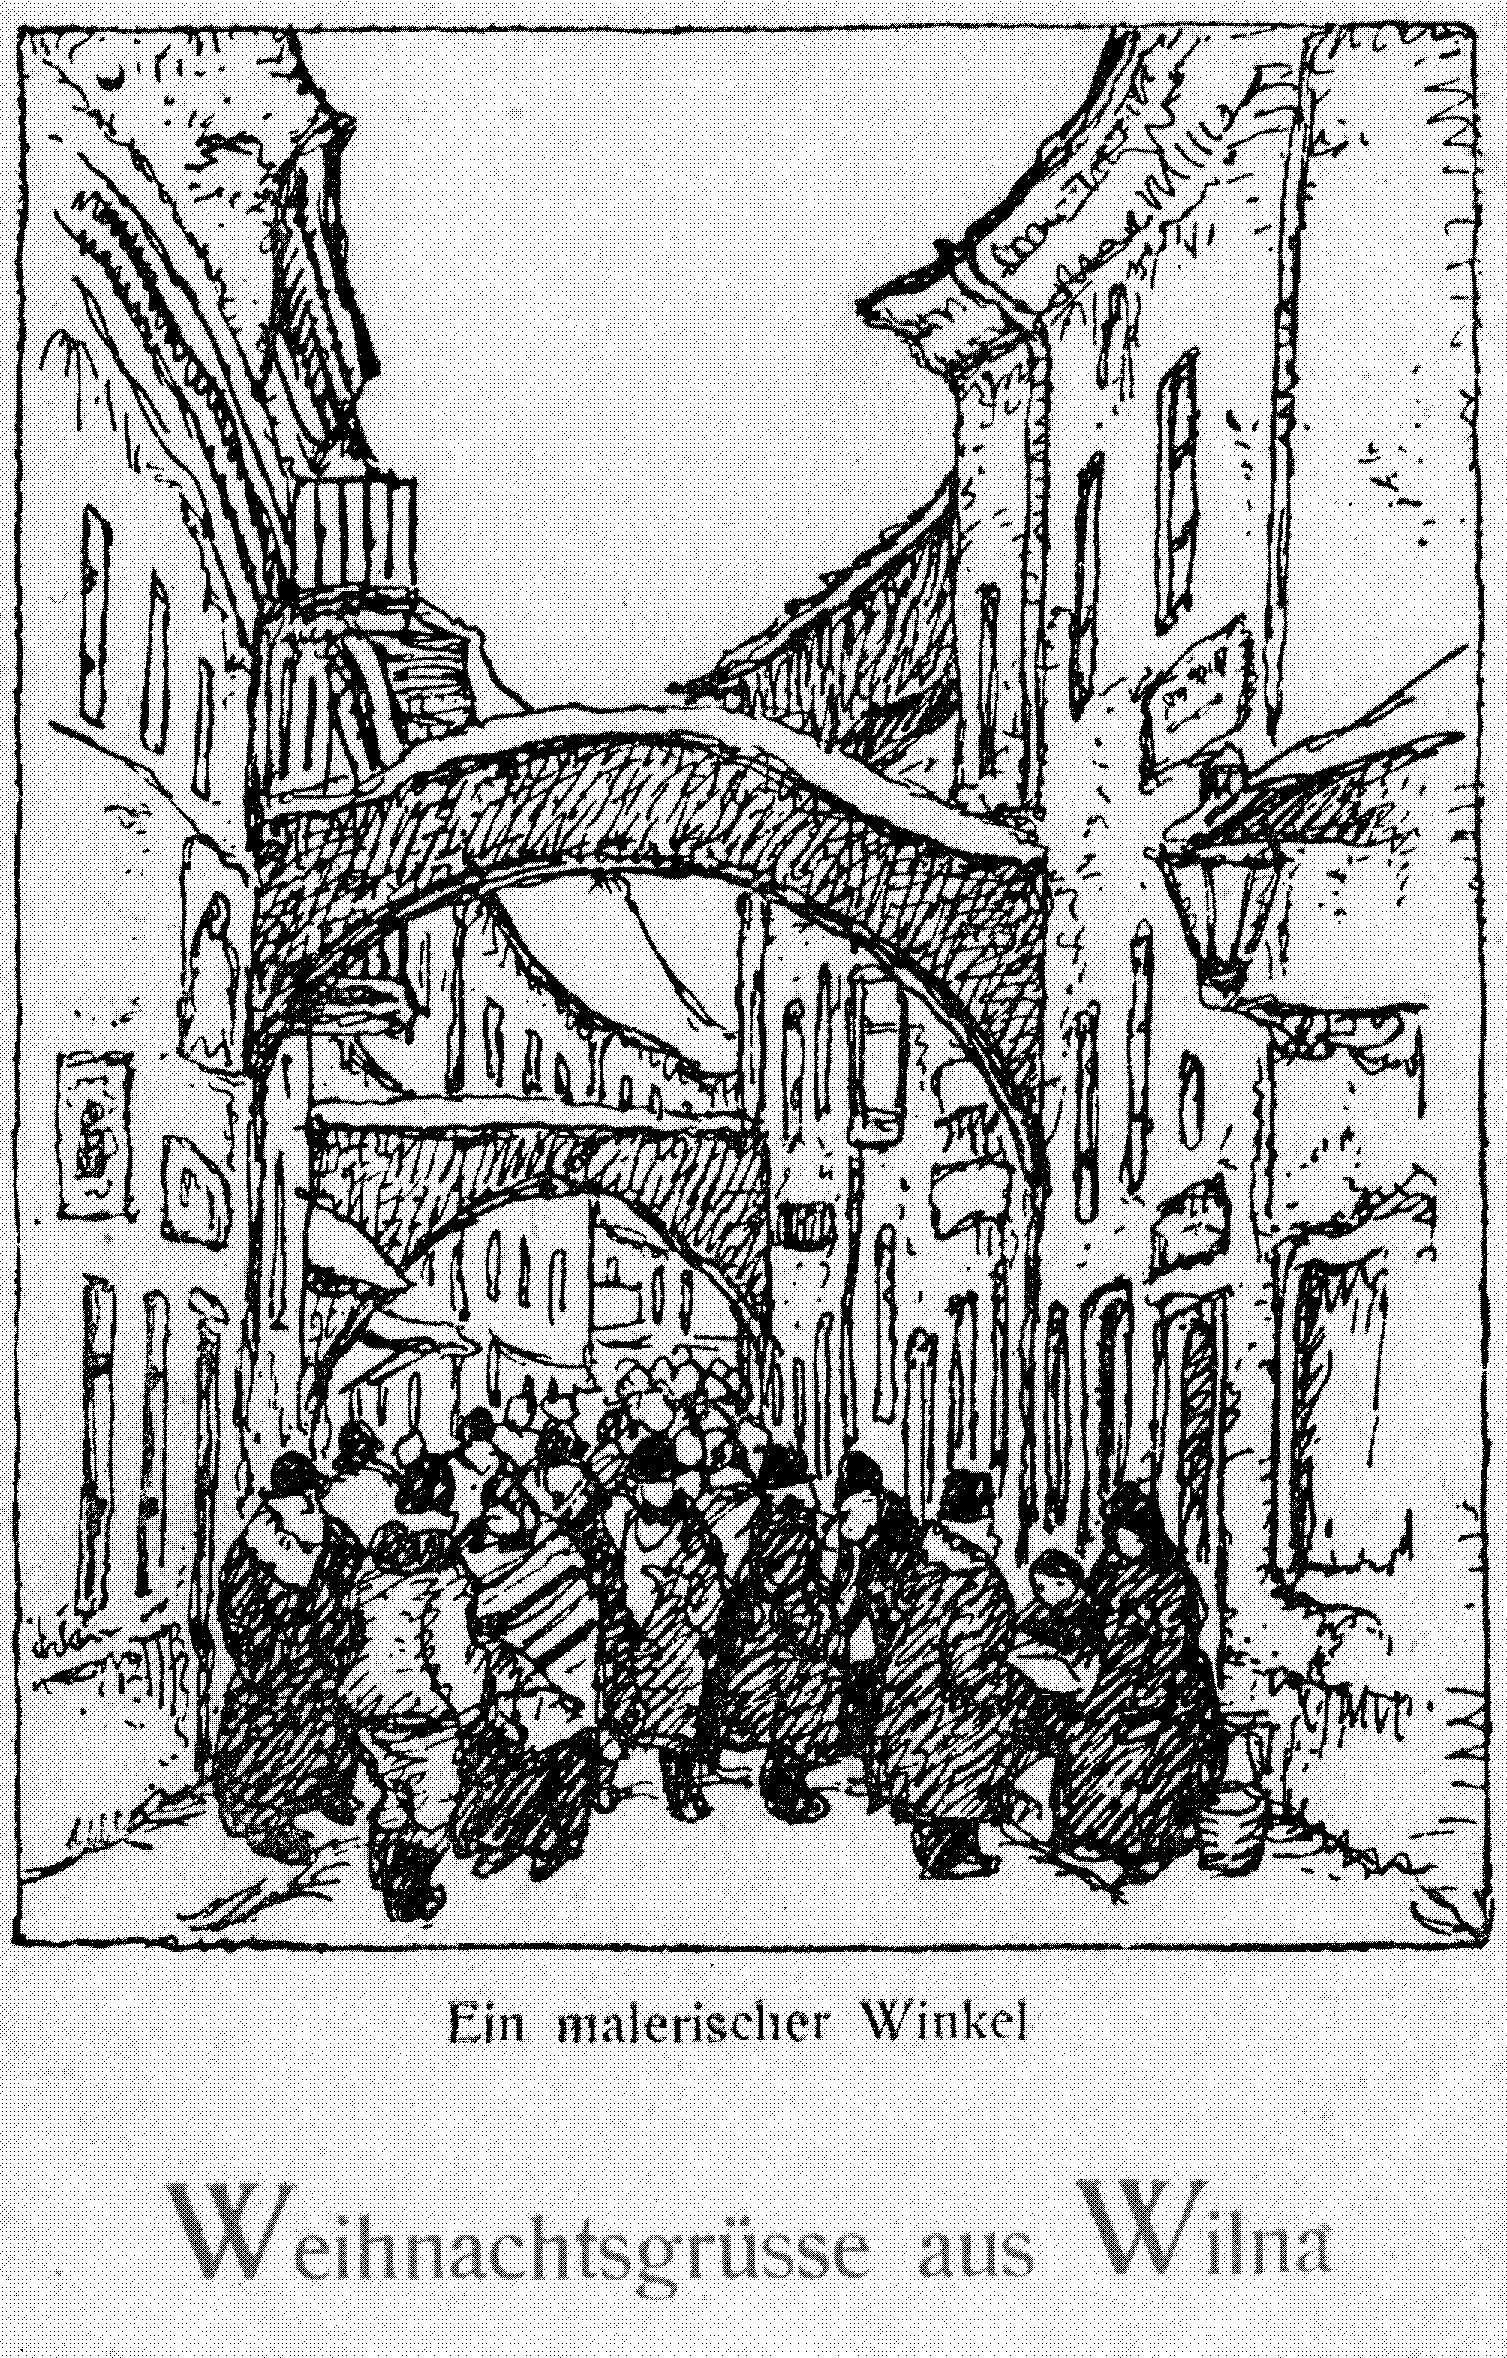
\includegraphics[width=10cm]{./ilustra-08.png} São Paulo\quad2021}
% \end{center}

\begin{figure}[!hp]
    \centering
    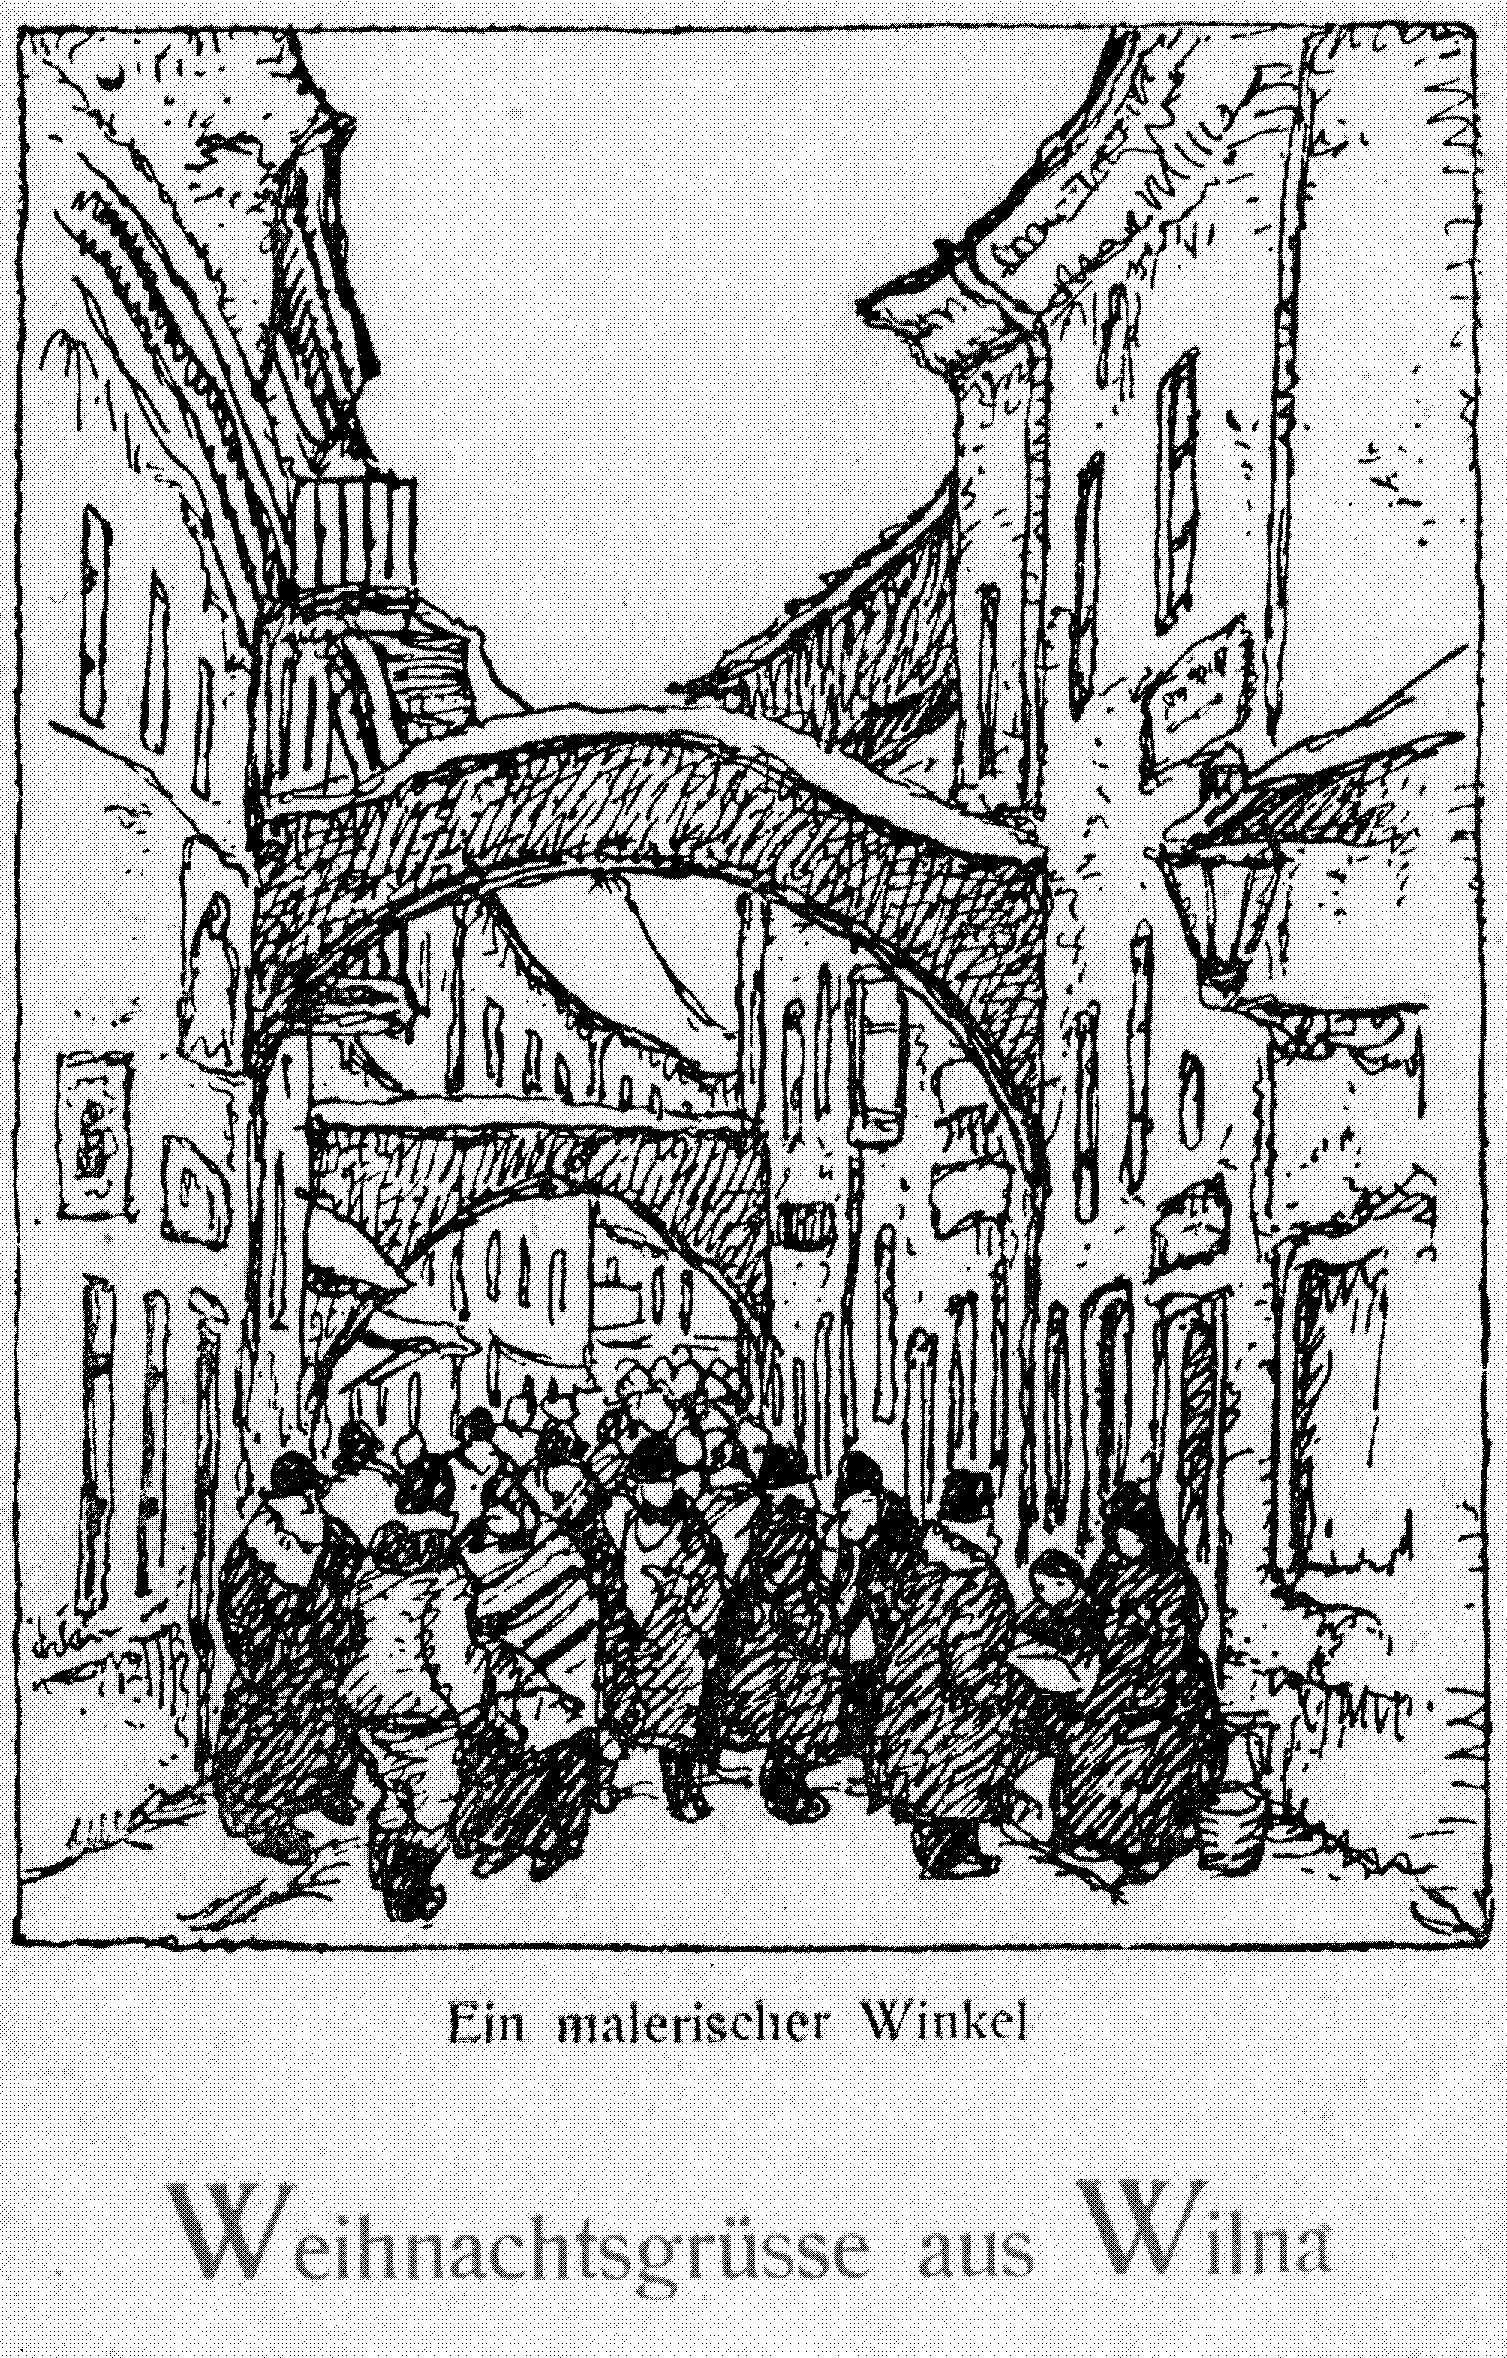
\includegraphics[width=\textwidth]{ilustra-08.png}
    \caption{Cartão postal que diz ``Recanto pitoresco: saudações de Natal de Wilna''.}
\end{figure}

Stephen Graham (1884--1975), outro jornalista britânico e, em suas
próprias palavras, grande admirador dos russos, passou o verão de 1915
em Vilna. Ficou enfeitiçado pela afeição e o respeito que teria
testemunhado entre duas nações rivais (poloneses e russos) e religiões
oponentes (católica e ortodoxa) no meio da frenética rotina diária em
tempo de guerra:

\begin{quote}
Estou na bela cidade antiga de Vilna, uma cidade de poloneses
bem"-educados, lar de várias dentre as antigas famílias nobres da
Polônia. Ela está agora atropelada por oficiais e soldados russos. Ao
longo da rua principal passa uma incessante procissão de tropas e,
olhando para baixo, pode"-se avistar um mar de pontas de baioneta
ondulando como junco ao vento. Quando se está deitado à noite na cama,
ouve"-se o estrépito dos passos dos soldados. Basta olhar pela janela
para assistir, por vinte minutos inteiros, à passagem de carroças e
canhões, ou pavoneando"-se por cima do pedregulho e da lama os cossacos
do Don, do Volga, da região dos Sete Rios. Nos dias da explosão
revolucionária, os poloneses mordiam os lábios de ódio à visão dos
soldados russos, praguejavam a cada respiração, arremessavam"-se com suas
pistolas e atiravam, lançavam bombas. Hoje eles sorriem, lágrimas
escorrem por suas faces; eles até mesmo dão vivas. Ninguém imaginaria
ver o dia em que os poloneses aplaudiriam as tropas russas marchando
pelas ruas de suas próprias cidades!

Os russos estão perdoados. Agora eles vêm para libertar os eslavos e
não, como antes, para os pisotear. Entre num restaurante e peça sua
comida em russo, você será coberto de sorrisos e tratado com reverência.
Ser russo é ser um \textit{amigo}. Os russos também, com toda aquela
atrapalhação de sentimentos de que só os povos eslavos são capazes,
demonstram bastante afeição pelos poloneses. Diz"-se que, desde a
proclamação do Grão"-Duque Nicolau, tem havido uma grande demanda por
gramáticas e dicionários poloneses por parte de russos que desejam
aprender o polonês. Eu, por exemplo, ao ler a proclamação, {[}e{]}
decidi na hora aprender um pouco de polonês, pois compreendi que a
Polônia de repente começava a contar.

Um espetáculo muito emocionante pode ser visto atualmente todo dia junto
ao Portão Sagrado de Vilna {[}Ostra Brama{]}. Por cima do portão, há uma
capela de portas escancaradas exibindo uma imagem da Virgem, ricamente
dourada e coberta de flores. De um lado, uma fileira de tubos plúmbeos
de órgão e, do outro, um padre. A música emana pela atmosfera junto com
o incenso e o som da reza. Lá embaixo, na ruela lamacenta, ajoelham"-se
homens e mulheres pobres segurando seus livros de orações. São
poloneses. Mas pelo portão passam incessantemente, todo dia e toda
noite, tropas russas rumo ao fronte. E quem se aproxima, cada soldado,
seja oficial ou não, ergue o chapéu e atravessa de cabeça descoberta
toda aquela multidão em prece. Isso é belo. Que a Rússia se comporte
sempre assim na presença da Mãe da Polônia.\footnote{Stephen Graham, \textit{Russia and the World}. Nova York: The Macmillan Company, 1915, pp. 145--147.} 
\end{quote}

%{[}figura 49{]}
%
%A Vilna russa, ca. 1900.

Essa miragem de harmonia nacional não incluía os judeus,
responsabilizados por todos os males da Rússia e também da Polônia. A
visão mais triste que se podia ter de Vilna, observou Graham, eram ``os
grupos de judeus pobres e sem teto'' que haviam sido forçados a fugir de
seus lares devido ao avanço da linha de frente, e ora afluíam ``para a
cidade segurando nas mãos tudo o que lhes restara.''\footnote{Ibid., p. 90.} A derrota do exército russo reativou o anti"-semitismo populista. ``Todos os russos pareciam reconhecer um judeu à primeira vista pelo
rosto e maneira de se mexer, tão intenso é o desprezo por sua figura.
Acho eu,'' afirmou o jornalista britânico, ``que isso se deva à oposição
fundamental do caráter judaico àquilo que o eslavo considera mais
precioso, {[}como o{]} descuido leviano, o desprezo para com posses
materiais, o amor ao vizinho, o misticismo.'' Malgrado portanto sua
trágica condição e seu estatuto marginal, os judeus, declarou Graham,
``com o talento que têm para o comércio, a simpatia pelo ocidentalismo e
o desdém pelo orientalismo, põem em perigo o ideal russo.''\footnote{Ibid., pp. 160--161.}

Graham via no sonho sionista de uma nação política a solução para a
alienação judaica. ``A dificuldade dos judeus é a de que aos poloneses
foi prometido algo enquanto poloneses, ao passo que aos judeus nada foi
prometido.'' A longo prazo, ``uma das possibilidades da guerra é a queda
do Império Turco e a libertação da Síria do jugo maometano.'' Diante de
tal resultado, refletiu o jornalista, ``a Palestina será desocupada, ou
pelo menos passível de um novo governo. Parece"-me que algo deveria ser
feito com vistas ao estabelecimento dos judeus na Palestina.'' Esse
esquema geopolítico radical poderia ser garantido pela recém"-reformulada
ordem mundial imperial do pós"-guerra, e ``tão logo um governo
{[}judaico{]} se forme, seria possível dar aos judeus a opção de
renunciar a seus diversos documentos nacionais europeus para se tornar
súditos judeus.'' Os judeus ``receberiam a proteção financeira e moral
do próprio governo. Se quiserem, poderiam tempestivamente instituir uma
democracia na Palestina; poderiam ter seu próprio exército e marinha
caso necessário. Isso seria uma enorme bênção para o mundo.'' Por seu
lado, o estado judaico salvaria o império tzarista, de alma russa e
ortodoxa, da humilhação nacional, pois ``o motivo principal que faz o
camponês russo considerar maldito o judeu é o fato de que ele não tem
sua própria terra. Por exemplo, quando os russos batiam em retirada para
a Polônia, perguntei a razão a um soldado raso. Sua resposta foi --- `Os
judeus nos traem\ldots{} eles nos perseguem e nos vendem a todo
canto.'"\footnote{Ibid., pp. 167--168.}

Geopolítica à parte, o fato de as forças alemãs se aproximarem de Vilna
imbuiu a mente de Graham com poderes mefistofélicos de uma criatividade
macabra. Embora aturdido pelas perspectivas futuras de um mundo
destroçado pela guerra, Graham compreendeu o significado histórico do
momento ao mencionar a cidade com o nome alemão. A conversão textual de
Vilna para \textit{Wilna} sinalizou o fim iminente da dominação russa:

\begin{quote}
Quantos dias passei em \textit{Wilna} chapinhando pela chuva! Encontrei"-me muito
mais próximo da guerra do que nunca antes. A guerra se tornava mais
íntima, criava e liberava um fluxo musical de pensamentos e impressões,
de modo que, sempre que caminhava, eu era como Abt Vogler ao órgão. O
tropel de milhares de passos rumo ao conflito e à morte, a música de
batalha, a paixão pela guerra e a dança da orgia, as cores e as
flâmulas, os emblemas e os símbolos, as vitórias e as terríveis
matanças, as conquistas de reinos, a humilhação de velhos deuses, e a
ereção de novos estados misturam"-se à alma numa música grandiosa,
apaixonada e apavorante.\footnote{Ibid., p. 110.}
\end{quote}

O lírico Bryusov também teve seu quinhão de emoções exacerbadas em
Vilna, mas de um ponto de vista diferente. O simbolista russo via a
inevitável onda de violência com os olhos de uma alma errante, cuja
decadente indiferença não fosse talvez mais do que uma máscara que
cobrisse uma aflição patriótica pela potencial perda de Vilna. Sob a
marcha trovejante do campo de batalha cada vez mais próximo, o poeta
vagueava pelas ruas da ``antiga Vilna russa'' com um sentimento
nostálgico de não haver volta:

\begin{verse}
De novo estou só --- um vagabundo sem teto,\\
Respirar contudo é tão fácil.\\
Onde agora, espírito meu inquieto,\\
Quais os próximos passos?\footnote{Bryusov, ``Em Vilna'', op.\,cit., p. 115.}
\end{verse}

\chapter{A intromissão alemã}

%\setlength{\epigraphwidth}{.45\textwidth}
\begin{epigraphs} 
\qitem{A guerra, apesar de sua destruição, ou, na verdade, devido a seu
penetrante horror, havia se transformado em força evocativa, estímulo
não para uma mudança social mas para a imaginação e a introspecção
pessoais, uma avenida que se abria para um novo e vital reino de
atividade.}{\textsc{modris eksteins}}
\end{epigraphs}

O primeiro sentinela alemão chegou às cercanias de Vilna em 10 Tishri
5676, de acordo com o calendário judaico; era o dia 4 de setembro de
1915, conforme a tradição (russa) juliana, e 17 de setembro no
calendário gregoriano (europeu ocidental). A data marcava um dos mais
sagrados dias judaicos, o Iom Kipur. No Dia do Perdão, que marca o fim
dos Dias de Arrependimento e o início do novo ano, perdoam"-se os pecados
humanos e se reafirma a aliança com Deus. Não se trata de uma festa
alegre, mas de um rito sóbrio de jejum e auto"-negação, que começa com
visitas ao cemitério e termina com a oração do \textit{N'iloh}. A palavra
hebraica \textit{N'iloh} significa fechamento, e se refere originalmente
ao fechamento dos portões do Templo. Mais tarde, após a destruição do
Templo, ela se imbuiu de um significado mais celestial, indicando o
fechamento do acesso ao Céu. É um momento de passagem do ano que sela o
destino humano.\footnote{Hayyim Schauss, \textit{The Jewish Festivals: History and Observance}. Nova York: Schocken Books, 1975, p. 154.}

Na véspera do Iom Kipur, as cidades judaicas do Leste europeu mergulham
no silêncio, como se todas as coisas mundanas se adiassem diante da
espera de um recomeço. Joseph Roth, escritor de credenciais vienenses,
comparou a cena do ritual do Iom Kipur à de um funeral judaico.
``Súbito, as ruazinhas escurecem porque de todas as janelas jorra a luz
das velas e as lojas são fechadas com urgência e uma precipitação
receosa --- e de maneira tão indescritivelmente hermética que se pode
imaginar que só voltarão a ser abertas no dia do Juízo Final.
{[}\ldots{}{]} Agora se acendem as luzes para todos os mortos; outras
são acesas para todos os vivos. Os mortos são deste mundo; os vivos, um
passo do além. Começa a grande oração. {[}\ldots{}{]} Das milhares de
janelas irrompe o grito de oração, interrompido por melodias calmas e
suaves do além, um canto ouvido do céu.''\footnote{Joseph Roth, \textit{The Wandering Jews}, trad. Michael Hofmann. Nova York: W.\,W. Norton, 2001, pp. 40--43. [Utilizou"-se a tradução de Marcus Tulius Franco Morais de \textit{Judeus em exílio}. São Paulo: Mundaréu, 2017, pp. 55--56. \textsc{n.\,t.}]}

Em 1915, o silêncio e as luzes palpitantes do Iom Kipur foram extintos
pelo caos da fuga russa e a iminente chegada dos alemães. O chefe da
equipe do distrito militar de Vilna era Paul von Rennenkampf, general
russo de origens aristocráticas báltico"-alemãs, que tinha, junto com as
forças alemãs e de outros países, liderado as tropas tzaristas na
supressão da Rebelião dos Boxers na China na virada do século \textsc{xx}. Nos
primeiros dias de guerra, o protestante Rennenkampf costumava rezar na
única igreja luterana de Vilna pela saúde do tzar e a vitória das armas
russas. Dessa vez, porém, a única esperança do alto comando tzarista era
retardar o inevitável: o Décimo Exército Russo, que se arrastava para
defender a Lituânia, não era páreo para o seu primo militar melhor
equipado, o Décimo Exército Alemão, que se projetou na direção de Vilna
no verão de 1915.

O desespero russo se tornava evidente nas ordens militares
contraprodutivas que tentavam fazer a cidade sumir do horizonte dos
alemães que avançavam. Em agosto, Vilna imergiu na escuridão e numa
letargia forçada: a iluminação pública foi eliminada e um apagão total
foi imposto às janelas de todas as casas viradas para o oeste. As
autoridades russas proibiram também todas as reuniões sociais e
atividades culturais, fixando severas restrições à circulação de civis
nas ruas. As medidas se revelariam inúteis; tão logo os alemães
atravessaram a linha de frente, mal protegida, a confusão, regida pelo
pânico, se instaurou.

\begin{quote}
Após a queda de Kowno {[}no fim de agosto{]}, \textit{Wilna} se preparou para a
evacuação. Havia muito as ruas já estavam lotadas de charretes de
refugiados que escapavam para o leste. Agora partia a administração
governamental, autoridades e funcionários se aglomeravam na estação
ferroviária, estalando de tantos pacotes e bagagem. Levavam consigo
estátuas e monumentos, símbolos do domínio tzarista. Paroquianos
circundavam as igrejas para evitar que levassem os sinos. A cidade foi
interditada, os serviços de correio e telefone foram cortados. À
aproximação dos alemães, logo ouviram"-se tiros de canhão vindo de três
lados. Zeppelins flutuavam por sobre a cidade, atirando bombas sobre as
ruas escuras. Os russos em retirada estavam decididos em deixar para
trás o menos possível aos alemães que avançavam. Ao cair da noite, as
margens da cidade eram incendiadas, pois o fogo `evacuava' o que a
ferrovia não conseguia. O governo procurava mobilizar todos os
reservistas locais, de maneira que a mão de obra não caísse nas mãos do
inimigo. Rapidamente, todas as medidas previamente planejadas se
diluíram em pânico. Equipes de incêndio punham fogo nas casas, fazendas
e casarões, saqueando, pilhando e empurrando as pessoas à força para o
leste. No dia 9 de setembro de 1915, o chefe do exército ordenou que
todos os homens entre 18 e 45 anos se retirassem junto com as tropas.
Quem fosse capturado pela polícia era enviado a centros de arrecadação
para ser transferido para longe. A intensificação do bombardeamento dos
Zeppelins, que danificaram a estação ferroviária e atiravam explosivos a
esmo, era o anúncio do fim. Os últimos regimentos russos e os cossacos
deixaram a passo de marcha uma cidade que parecia morta. No intervalo
onírico antes da chegada dos soldados alemães, a vida começou lentamente
a se refazer, com a organização, por parte dos habitantes locais, de
comitês cívicos, polícia e jornais. O último adeus das forças tzaristas
foi o som de explosões, causado por pontes mandadas aos ares.\footnote{Vejas Liulevicius, \textit{War Land on the Eastern Front: Culture, National Identity and German Occupation}. Cambridge: Cambridge University Press, 2001, p. 19.} 
\end{quote}

%{[}figura 51{]}
%
%``Captura de \textit{Wilna}, cidade russa sede de governo, agosto de 1915.''
%Nesse cartão postal comemorativo, tanto a data da conquista alemã da
%cidade bem como a perspectiva do desenho estão incorretas: \textit{Wilna} foi
%tomada pelos alemães em setembro e o leito do rio, na verdade, corre na
%direção contrária à que está retratada.

Nas primeiras horas do dia 19 de setembro, enquanto os últimos soldados
russos fugiam da cidade, cento e vinte anos de domínio tzarista chegavam
ao fim. Por um breve momento, residentes locais assumiram o poder, até o
exército alemão chegar e exigir os despojos.

O alto comando alemão, assim como Napoleão em 1812, viam na tomada de
\textit{Wilna} uma vitória estratégica. Ela abria, segundo o general Erich von
Ludendorff, a possibilidade de se terminar a guerra com ``uma derrota
decisiva dos exércitos russos.''\footnote{Erich Ludendorff, \textit{My War Memories}, vol. 1. Londres: Hutchinson \& Co., 1919, p. 175.} Apesar das grandes esperanças de Berlim, o avanço alemão na Frente Oriental não
trazia nenhuma perspectiva de paz. No fim de 1915, a frente teuto"-russa
se estabeleceu ao longo das margens norte e oriental da Lituânia,
tornando \textit{Wilna} uma localidade de fronteira.

A partir dos territórios ocupados da região \textit{Severo"-zapadnyi}
(Noroeste) do império russo, os alemães criaram o território
\textit{Ober"-Ost} (Leste Superior). Dentro de seus confins, o fracassado
estratega militar Ludendorff --- àquela altura nomeado chefe do comando no
Oriente --- se concentrou no grandioso ``trabalho alemão para a
civilização.'' ``A monotonia da guerra de trincheira,'' escreveu o
general, ``foi aliviada sobremaneira pelo emprego dos homens na
indústria. Simpatizei com esse sentimento, e fiquei contente em
encontrar um novo campo em que pudesse servir à Pátria. Uma atividade
muito estimulante me coube, e absorveu toda a minha atenção. Sentimos
que trabalhávamos pelo futuro da Alemanha, mesmo em terra
estrangeira.''\footnote{Ibid., p. 243.}

Na Lituânia, Ludendorff vislumbrava o futuro da \textit{Vaterland} à luz
heroica das tribulações nacionais alemãs. Nessa perspectiva, a visão de
Kowno, onde estabeleceu o quartel"-general militar da região
\textit{Ober"-Ost}, se transformava num panorama histórico das obras da
civilização alemã:

\begin{quote}
Na margem mais distante do Niemen, ergue"-se a torre de um velho castelo
alemão dos Cavaleiros Teutônicos, símbolo da civilização alemã no
Oriente e, não longe dele, há um memorial dos planos franceses para a
conquista do mundo --- aquela colina em que Napoleão esteve em 1812,
enquanto observava seu grande exército cruzando o rio.

Minha mente foi invadida por memórias históricas irresistíveis; ordenei
que se retomasse, no território ocupado, aquele trabalho civilizatório a
que os alemães haviam se dedicado naquelas terras por tantos séculos.
Sua população, formada como é por um misto de raças, jamais realizaria
nada por vontade própria e, abandonada a si mesma, sucumbiria à
dominação polonesa. [\ldots{}] Um futuro brilhante de prosperidade
garantida parecia se abrir à nossa Pátria.\footnote{Ibid., pp. 210--212.}
\end{quote}

Unir a futura prosperidade da Alemanha à história do território
conquistado era mais exitoso que fazê"-lo servir às necessidades
presentes do império. Apesar da proximidade histórica e geográfica, a
\textit{Ober"-Ost}, aos olhos dos oficiais alemães, era \textit{terra
incognita}:

\begin{quote}
O país se encontrava devastado devido à guerra, e só onde estabelecemos
zonas de ocupação por algum tempo é que havia algo que se parecesse com
ordem. [\ldots{}] A população, exceto a de origem alemã, se manteve à
distância de nós. Os distritos alemães, em especial os bálticos, deram
as boas vindas a nossas tropas. Os letões eram oportunistas, e
aguardavam o desenrolar dos acontecimentos. Os lituanos acreditavam que
chegara o momento da libertação e, quando os bons tempos que haviam
imaginado não se materializaram, devido às cruéis exigências da guerra,
eles se tornaram de novo desconfiados e se voltaram contra nós. Os
poloneses eram hostis, pois temiam, com certa razão, a instauração de
uma política pró"-lituana da nossa parte. Os rutenos brancos não tinham
importância, pois os poloneses os haviam espoliado de sua nacionalidade
e lhes dado nada em troca. No outono de 1915, pensei que seria bom ter
uma ideia da distribuição dessa raça. Em princípio, eram literalmente
impossíveis de ser encontrados. Depois, descobrimos que eram um povo
amplamente disperso, aparentemente de origem polonesa, mas de um nível
tão baixo de civilização que seria necessário muito tempo para que
pudéssemos fazer algo por eles. Os judeus não sabiam que comportamento
adotar, mas não nos criavam problemas, e éramos pelo menos capazes de
conversar com eles, o que era quase impossível com os poloneses,
lituanos e letões. As dificuldades linguísticas pesaram muito a nosso
desfavor e não podem ser subestimadas. Devido à escassez de obras alemãs
de referência sobre o assunto, sabíamos muito pouco sobre o país e o
povo, e nos encontramos num mundo estranho. Numa região tão grande
quanto a Prússia Oriental e Ocidental, a Pomerânia e Posen todas juntas,
víamo"-nos diante de uma tarefa espantosa. Tínhamos que construir e
organizar tudo do zero.\footnote{Ibid., pp. 221--222.}
\end{quote}

%{[}figura 52{]}
%
%\textit{Wilna}: panorama a partir da Colina do Castelo.

Como no passado, a reorganização dos territórios conquistados começava
com o saque, o que, nas palavras de Ludendorff, ``foi realizado da
maneira mais ordenada possível, embora um pouco de confusão tenha sido
inevitável.''\footnote{Ibid., p. 211.} A confusão, entretanto, não
deveria ser imputada à inadequação ou ineficiência da ordem alemã, mas
às ``lamentáveis condições impostas pelas exigências da guerra.''
Contudo, ``para o indivíduo que sofre, não interessa \textit{como} perde
sua propriedade. Ele nada entende das necessidades da guerra e,
portanto, está sempre pronto a falar dos bárbaros métodos militares do
inimigo.''\footnote{Ibid., pp. 211--212.}

Enquanto Kowno alimentava sonhos de glória, \textit{Wilna} os desafiava, na
medida em que ``dificuldades extraordinárias ainda precisavam ser
superadas.''\footnote{Ludendorff, \textit{My War Memories}, vol. 2. Londres: Hutchinson \& Co., 1919, p. 154.} Tais dificuldades surgiam nem tanto da inabilidade alemã em controlar as exigências da guerra,
como da intrincada localização geográfica da cidade. Entre Kowno e
\textit{Wilna}, observou o escritor Alfred Brust (1896--1934), que chegou à
Lituânia integrando as fileiras do exército de ocupação, ``a dogmática
divisão de Ocidente e Oriente perde o sentido, pois tudo --- religiões,
línguas, culturas, povos, histórias e estilos arquitetônicos --- aqui se
entrelaça.''\footnote{Alfred Brust, \textit{Die verlorene Erde}, conforme citado em Dietmar Albrecht, \textit{Wege nach Sarmatien -- Zehn Kapitel Preussenland: Orte, Texte, Zeichen}. Munique: Martin Meidenbauer, 2006, p. 174.} Kowno, notou Richard Dehmel, censor da imprensa alemã nos territórios do \textit{Ober"-Ost}, ``pouco difere das cidades
provincianas da Prússia Oriental\ldots{} e o panorama da cidade me faz
lembrar de Veneza com suas lagunas ao invés de Moscou ou Petersburgo. A
verdadeira Rússia só começa em \textit{Wilna}, a cidade de uma centena de igrejas
e um milhar de bordéis. Mesmo ali, porém, predominam os espíritos
lituano e polonês.''\footnote{Richard Dehmel, \textit{Zwischen Volk und Menschheit: Kriegstagebuch}, conforme citado em Albrecht, op. cit., p. 173.}

Segundo as estatísticas russas, Vilna tinha quase 200 mil habitantes
logo antes da guerra, aproximadamente 40\% dos quais eram judeus, mais
de 30\% poloneses, cerca de 20\% russos, enquanto o resto consistia em
pequenas minorias de lituanos, bielorrussos, alemães e tártaros. A
situação demográfica se modificou dramaticamente assim que começou, na
primavera de 1915, a contra"-ofensiva alemã. Embora a maioria dos russos
houvesse evacuado a cidade, ela foi inundada por milhares de refugiados
do interior da Lituânia. Muitos desses refugiados eram judeus forçados a
abandonar suas casas sob ordens da administração russa, por serem
potencialmente ``simpáticos ao inimigo.''

A ocupação alemã de Vilna foi inicialmente anunciada em três línguas:
alemão, russo e polonês. O General Pfeil, comandante do exército de
ocupação, alardeou o fim da tirania tzarista: ``As forças militares
alemãs impeliram o exército russo para fora do território da cidade
polonesa de \textit{Wilna}. Várias divisões do exército alemão entraram na
notável e lendária cidade de \textit{Wilna}. A cidade foi sempre uma pérola dos
domínios poloneses\ldots{} e a Alemanha é amiga desses
domínios.''\footnote{Petras Čepėnas, \textit{Naujųjų laikų Lietuvos istorija}. Vilna: Mokslo ir enciklopedijų leidykla, 1992, p. 27.} No dia seguinte, Pfeil recebeu a visita de representantes das comunidades lituana e judaica, que fizeram objeções ao fato de os
alemães terem situado a cidade nos domínios poloneses. \textit{Wilna}, explicaram
os delegados, era uma cidade poliglota, capital da Lituânia, com uma
população judaica predominante. Em seguida, o general institucionalizou
um multilinguismo semi"-oficial. Como a língua alemã substituiu o russo
como \textit{lingua franca} oficial, a nova administração reconheceu
também o uso público de línguas adicionais: polonês, iídiche, lituano e
bielorrusso.

A fim de esclarecer a difusão nacional e as perspectivas futuras do
lugar, os alemães iniciaram a dominação com um recenseamento. Contaram
um total de 140.840 habitantes, divididos em diversos grupos
linguísticos baseando"-se no princípio da língua materna, com o polonês
(50\%) e o iídiche (44\%) afirmando"-se com as maiores quotas. Juntos,
falantes de lituano, russo e bielorrusso contavam menos de 10\% da
população, com os russos sofrendo a maior queda nos números. Havia
também cerca de mil alemães (menos de 1\%) entre a população civil. A
afiliação religiosa da cidade espelhava sua segregação étnica, com mais
da metade da população sendo católica e 43\% pertencendo à fé mosaica.
Ademais, havia minúsculas minorias greco"-ortodoxas e
protestantes.\footnote{Wiktor Sukiennicki, \textit{East Central Europe during World War \versal{i}: from Foreign Domination to National Independence, vol. 2}. Nova York: Columbia University Press, 1984, p. 161.}

As estatísticas revelaram uma paisagem demográfica não muito bem
recebida em Berlim. Entre os povos da região ocupada, os alemães
favoreceram claramente os lituanos, que consideravam ser menos ativos do
ponto de vista político e cultural e, portanto, mais complacentes com o
poder alemão. Enquanto a administração imperial tencionava estabelecer
um principado lituano avassalado, Ludendorff se preocupava com o fato de
que ``qualquer príncipe em Vilna acolheria a nobreza polonesa em sua
corte, os oficiais do exército seriam poloneses, assim como também a
maioria das autoridades civis.'' Como resultado, só ``os alemães
prussianos seriam capazes de manter a Lituânia para os lituanos, e
providenciar oficiais militares e autoridades civis, que os lituanos
seriam incapazes de prover em números suficientes. Estados capazes de
existência independente não são produzidos por palavras de ordem
políticas, nem pequenas nações conseguem assim se manter vivas. Não me
contentava de maneira alguma, portanto, com soluções vagas, que pareciam
ser tão perigosas para o futuro da Alemanha.''\footnote{Ludendorff, op. cit., \textit{My War Memories}, vol. 2, pp. 153--155.}

Essa intensa preocupação com o futuro político da cidade não trouxe
alívio para seus habitantes. A administração alemã colocou a Lituânia
sob ordens de requisição de alimentos e instituiu exigências de trabalho
pesado aos residentes urbanos. Com a redução do abastecimento de comida,
ondas de epidemias varreram a cidade. A fim de evitar a disseminação de
doenças, os militares rotineiramente proibiam a realização de feiras e
determinavam a desinfecção das lojas. Procissões funerárias foram também
proscritas e ``todos foram forçados a se vacinar contra cólera, sarampo
etc., proibidos de mudar de casa, e as prostitutas foram registradas e
examinadas.''\footnote{Petras Klimas, \textit{Iš mano atsiminimų}. Vilna: Lietuvos enciklopedijų redakcija, 1990, p. 45.} Contudo, tais medidas fracassaram em salvar a cidade:

\begin{quote}
Os russos haviam deixado um legado de cólera, que fora erradicado em
novembro de 1915; mas a privação física daqueles dezesseis meses gerou
uma epidemia de tifo, que grassou desde o início de 1917 ao longo de
nove meses, acompanhada parcialmente por um surto de disenteria. No
verão daquele ano, era raro uma casa em Vilna não ostentar um sinal
vermelho avisando ao público de que a contaminação chegara ali. Casos
urgentes costumavam ter de esperar dois ou três dias até que a
ambulância pudesse transferi"-los para o hospital de isolamento, e em
geral ela chegava tarde demais. As pessoas tinham que fazer fila para
obter caixões. Os carros fúnebres eram incapazes de fazer frente à
demanda, de maneira que os caixões eram enfileirados no pavimento, à
espera das carroças sobre as quais eram depois empilhados. Vilna se
transformou numa cidade dos mortos, e os que ainda por ela perambulavam
se sentiam como meros fantasmas.\footnote{Israel Cohen, \textit{Vilna}. Filadélfia: The Jewish Publication Society of America, 1992, p. 366.} 
\end{quote}

A administração alemã teve mais sucesso em salubrizar as ruínas
topográficas e cartográficas russas da cidade. A maioria dos nomes de
ruas foram traduzidos do russo para o alemão; mas, estranhamente, a
Praça Muraviev passou a ser chamada \textit{Napoleon Platz}. A igreja
ortodoxa russa de São Nicolau (antiga igreja católica de São Casimiro)
foi convertida num templo protestante a fim de abrigar as necessidades
espirituais do Décimo Exército Alemão. O tzar Nicolau \versal{ii} havia orado ali
por bênçãos celestes durante os primeiros dias da guerra --- o Kaiser
Wilhem \versal{ii} fez o mesmo ao passar em revista a Frente Russa no verão de
1916.

\asterisc

Apesar da proximidade com a linha de frente, a população multinacional e
o futuro incerto, os alemães rapidamente arrogaram a cidade para si. À
pluralidade linguística da imprensa local, o comando militar alemão
adicionou o próprio jornal, o \textit{Wilnaer Zeitung}. Seu primeiro
número foi publicado em 20 de janeiro de 1916, com uma manchete sobre a
capitulação de Montenegro. Entretanto, o artigo principal levava
simplesmente o título de \textit{Das deutsche Wilna}, ``A Vilna alemã''.

O \textit{Wilnaer Zeitung} foi um produto da ocupação, publicado pelo
Décimo Exército para um público"-alvo de soldados alemães estacionados na
cidade ou ao redor dela. Em suas páginas, notícias militares se
misturavam tranquilamente a estórias mundanas do mundo civil, e críticas
de peças locais do teatro alemão, iídiche, polonês e lituano tomavam
tanto espaço quanto os relatórios dos avanços estratégicos do exército
alemão. Toda semana, o jornal publicava o horário dos trens da estação
ferroviária de \textit{Wilna} --- indicador do seu papel como importante eixo de
transporte, conectando a \textit{Vaterland} alemã à Frente Oriental. Em
março de 1916, a publicação iniciou uma série de artigos ao gênero do
folhetim --- vinhetas do quotidiano da vida urbana --- sob o título
\textit{Wanderstunden in Wilna}, ``Passeios por \textit{Wilna}''. ``Essas vinhetas,''
explicou o editor, ``são dirigidas aos soldados alemães de licença, que
têm o desejo de explorar melhor a cidade''. Eram publicadas uma vez por
semana e, inicialmente, assumiram a forma de breves orientações
turísticas, indicando atrações locais aos soldados erráticos: a
catedral, as igrejas, o bairro judaico, ou os mais interessantes
distritos periféricos da cidade. Em poucas semanas, o tom e o formato de
tais artigos anônimos se modificaram --- transformando"-se, de notas de
jornal instrutivas e descritivas, em exemplos de escrita literária.

O \textit{Wilnaer Zeitung} era co"-editado por Paul Otto Heinrich Fechter,
crítico cultural e literário, que, em 1914, escreveu um dos primeiros
livros sobre o Expressionismo como corrente artística. Fechter nasceu em
1880 na cidade de Elbing, perto de onde também era Forster, na Prússia
Ocidental, numa família de negociantes de madeira com estreitas conexões
comerciais com a Lituânia. Como tantas outras pessoas talentosas de seu
tempo, ele se sentiu atraído por Berlim, a irrequieta capital do Império
Alemão, onde estudou arquitetura, matemática e física. Aos 26 anos de
idade, doutorou"-se em filosofia com uma tese sobre a dialética. Uma
profissão acadêmica, porém, não se enquadrava nas intenções de Fechter,
de modo que passou a se dedicar ao jornalismo criativo, tornando"-se um
editor de folhetim, primeiro em Dresden e depois em Berlim. Fechter
escreveu imensamente sobre teatro e literatura modernos e, no papel de
um dos primeiro defensores do Expressionismo, foi totalmente absorvido
pela experiência espetacular e frenética da vida de uma
metrópole.\footnote{Paul Fechter morreu em 1958 em Berlim Ocidental.}

Durante a guerra, Fechter evitou o serviço militar ativo, sem porém
deixar de compreender de perto as técnicas modernas de guerra. (O irmão
mais novo, Hans Fechter, foi um dos primeiros pilotos de submarino da
flotilha imperial alemã.) Designado ao cargo de escritor de folhetim no
\textit{Wilnaer Zeitung}, Fechter procurou utilizar sua verve criativa
tanto quanto possível. As exigências propagandísticas e a severa censura
do jornal militar ofereciam pouco espaço de manobra: seu conhecimento da
arte expressionista, do teatro moderno e da literatura de alto nível
acabava ficando guardado para si. A imaginação de Fechter, contudo,
encontrou um minúsculo nicho literário nas narrativas dos
\textit{Wanderstunden in Wilna}, onde foi capaz de combinar a sensibilidade
artística de um \textit{flâneur} metropolitano com a questão restritiva
dos assuntos militares. As vinhetas urbanas foram reunidas num guia e
publicadas sob o mesmo título pelo jornal, como sendo de autoria de Paul
Monty, pseudônimo de inspiração inglesa utilizado por Fechter. O livro
ganhou três edições consecutivas --- a última em 1918, ao término da
ocupação alemã --- e foi oficialmente aprovado pelo comando militar dos
territórios do \textit{Ober"-Ost}.

Monty/Fechter inicia sua jornada por \textit{Wilna} como uma fuga às
responsabilidades militares, o que, ironicamente, abre a possibilidade
de uma conquista mais ampla:

%{[}figura 53{]}
%
%Soldado alemão flâneur em \textit{Wilna}, 1916.

\begin{quote}
Neste mundo, o direito de conquistar cidades estrangeiras é um
privilégio reservado apenas aos poucos governantes e líderes militares
corajosos, embora todo viajante possa exitosamente dominar cidades
desconhecidas caso se aperfeiçoe na arte de andar sem destino. Se o
viajante for um estrategista inteligente, ele decerto consultará vários
mapas e crônicas antes de se aventurar numa cidade estrangeira. Se o
viajante for um artista --- e andar sem destino é a forma mais livre da
arte --- ele abordará a cidade a partir de uma perspectiva completamente
diferente. Sem qualquer hesitação, o andarilho urbano permitirá que o ar
fresco o guie pelas ruas desconhecidas da cidade remota. Essa maneira de
viajar tem o poder de destruir todo tipo de fortificação. Felizmente
para o viajante, nossa velha e boa \textit{Wilna} é abençoada por uma brisa
perpétua, criando condições perfeitas para um passeio sem fim por suas
ruas e praças.\footnote{Paul Monty, \textit{Wanderstunden in Wilna}. Vilna: Verlag der Wilnaer Zeitung, 1918, p. 76.} 
\end{quote}

Essa vivência de \textit{Wilna} testemunha uma história não"-realizada de
modernidade e juventude, atributos externos do soldado alemão. ``A
história da cidade,'' anuncia o guia, ``não tem como ser resumida por
crônicas nem livros. A idade do lugar se reflete da maneira mais
evidente pelo modo como ele mesmo se expressa. As funções modernas da
cidade se definem por suas provações históricas e energia contemporânea.
Se o rosto de uma pessoa reflete sua vida e destino, então o caráter de
uma cidade se torna visível no traçado geral do lugar.'' ``O mapa de
\textit{Wilna},'' prossegue o autor do guia, ``se parece com o rosto de um velho
longevo que jamais verdadeiramente experimentou os mais importantes e
cruciais momentos da vida.''\footnote{Ibid., p. 9.} Segundo o autor, a
cartografia em processo de envelhecimento revelava um padrão de
regressão histórica:

\begin{quote}
\textit{Wilna}, assim como muitas outras cidades antigas, passou por vários
incêndios devastadores. Tanto tempos difíceis como a falta de líderes
habilidosos sempre comprometeram a total recuperação da cidade. Foi
assim que o rosto velho e enrugado da cidade amadureceu: como não havia
um plano geral, cada casa foi construída sem considerar os outros
edifícios. Assim, uma linha reta se tornava curva e, com o tempo, e
devido ao terreno colinoso, essas curvas se transformaram numa teia.
Comparando com \textit{Wilna}, a trama intrincada e entrelaçada das ruas antigas
de Roma parece coerente e racional.\footnote{Ibid., p. 10.}
\end{quote}

Esse esqueleto urbano retorcido, continua Monty, ``com ruas tortuosas e
enlaçadas, não apresenta uma hierarquia de logradouros claramente
demarcada,'' não tendo, portanto, ``um coração que regule a vida
quotidiana.'' Em suma, ``o mapa da cidade implora por uma incisão,'' uma
cirurgia cartográfica radical que faça penetrar a energia da Europa
moderna pelas artérias urbanas entupidas de uma \textit{Wilna} envelhecida.

A regeneração da cidade deveria começar pela eliminação das ruelas
estreitas e cheias de meandros da cidade velha e o alargamento das
principais vias públicas. Novas avenidas deveriam ser traçadas e praças
urbanas em coma precisavam ser reavivadas; os rios rebeldes deveriam ser
demarcados e a natureza que tudo engolia tinha de ser domesticada. O
mais importante era que a cidade generosamente abraçasse a estação
ferroviária --- elo essencial da máquina de guerra alemã. Para esse
propósito, ``as velhas ruas curvas têm de ser endireitadas e alargadas
de maneira que o centro da cidade tenha acesso direto à estação de trem.
Esse corte nítido criará um eixo urbano principal que harmonizará de
imediato o mapa funcional da cidade.'' Em um tom satírico, Monty opina
que o lendário realizador da modernidade urbana ``Barão Haussmann,
criador dos bulevares parisienses, encontraria bastante inspiração para
trabalhar.'' Mas até que esse momento mágico da transformação moderna
chegue, aqueles que visitarem \textit{Wilna} ``terão de tolerar a lógica quase
inexistente do traçado das ruas, pois navegar por esse incompreensível
labirinto urbano só é possível aceitando"-se sua coerência
anacrônica.''\footnote{Ibid., pp. 10--12.}

Como o próprio Monty admitiu, ao seguir essa lógica, o viajante
inevitavelmente se encontrará vagueando sem rumo por um labirinto de
lugares impossíveis de identificar. ``Em muitas cidades, podemos nos
orientar lembrando"-nos de nomes de ruas e observando a relação
geográfica dentre elas. Não é assim que funciona em \textit{Wilna}, onde quem a
visita é obrigado a cruzar a mesma rua diversas vezes até conseguir
distingui"-la das outras.''\footnote{Ibid., p. 17.} Ademais, embora a
cidade possua muitas ``praças grandes e pequenas, encantadoras durante a
primavera, não há uma praça principal que possa unificar a vida da
cidade. Todas as praças, assim como as ruas curvas da cidade, brotaram
espontaneamente, sem qualquer função pública clara em mente.'' Não há
nada em \textit{Wilna}, por exemplo, que pudesse se comparar à ``Marktplatz de
Hildesheim, ao Altmarkt de Dresden ou à Piazza de Florença.'' A imensa
praça da catedral de \textit{Wilna} é ``uma aparente protuberância sem delineio,
limitada por um lado pela cidade mas, por outro, solta no mato.'' Não é
``nem mesmo uma praça, e sim um parque revolto, um túnel verde que se
projeta até a Colina do Castelo e funde a cidade aos jardins privados
que a cercam.''\footnote{Ibid., p. 13.} A intromissão da natureza
restringe todas as atividades modernas; como resultado, ``o progressivo
ritmo urbano contemporâneo ainda precisa invadir as praças de \textit{Wilna}, até
agora governadas pela letargia penetrante do passado.''\footnote{Ibid., p. 15.}

Monty chama a atenção para a diferença entre aquilo que encontra um
observador que simplesmente passa pela cidade e o que se revela a quem
adentra no quebra"-cabeças. ``Qualquer pessoa que olhar do alto para a
cidade, a partir das colinas que a rodeiam ou de edifícios mais altos,
como o majestoso quartel perto da estação ferroviária,'' afirma o guia,
``poderá notar que \textit{Wilna} é uma cidade grande. Muitos viajantes, que por
aqui se demoram por apenas algumas horas em seu trajeto rumo a destinos
mais importantes, testemunham apenas o espetáculo nada atraente de uma
pobre cidade provinciana, de ruas mal pavimentadas. Essa primeira
impressão, que é soturna, extingue qualquer desejo por descobrir a
cidade. Mas só imergindo em seu território meândrico é que se torna
possível explorar a intrincada vida multicolorida da cidade.''\footnote{Ibid., p. 16.} Por conseguinte, Monty convida os viajantes a se tornarem \textit{flâneurs}, utilizando seu texto como diagrama para encontros
urbanos potencialmente intrigantes. Em outras palavras, na ausência de
um bom mapa ou de um traçado topográfico moderno, é só por meio de uma
perambulação a esmo que \textit{Wilna} é capaz de se enquadrar no espírito
progressivo da vida moderna.

O público"-alvo do autor e, portanto, as pessoas que potencialmente
realizariam o ``trabalho de campo'' dos itinerários urbanos sugeridos,
eram os soldados da linha de frente estacionados em \textit{Wilna} e arredores. O
guia não contém informações turísticas práticas, como por exemplo
detalhes específicos relativos a hospedagem, alimentação e transporte,
pois os soldados não necessitavam de tal conhecimento. Suas acomodações
e comida eram providas pelo exército. Havia algumas outras publicações
em alemão, publicadas pela mesma gráfica do Décimo Exército, que se
concentravam especificamente na paisagem arquitetônica e histórica da
cidade, sublinhando sua afiliação à cultura teutônica.\footnote{Vide, por exemplo, Paul Weber, \textit{Wilna: eine vergessene Kunstsstätte}. Vilna: Verlag der Zeitung der 10. Armee, 1917.} Por outro lado, Monty procurava familiarizar os leitores com \textit{Wilna} através de uma série de
excursões aleatórias e expressionistas, instigando um maior nível de
liberdade pessoal e imaginação.

%{[}figura 54{]}
%
%Mapa de \textit{Wilna} e arredores, com destaque às artérias principais cortando
%a cidade, 1917.

Com a guerra se tornando mais brutal e se movendo para além das
imediações do mundo civilizado, pacífico e familiar, o soldado alemão,
nas palavras do historiador Eksteins, passou a perder gradualmente sua
afiliação ao ambiente cultural de sua terra natal e a se transformar num
personagem ambíguo. ``Como agente tanto da destruição como da
regeneração, da morte e do renascimento, o soldado tendia a se ver como
personalidade `fronteiriça', paladino da mudança e de uma nova vida. Ele
encarnava um viajante que, para cumprir ordens, havia zarpado para os
limites da existência, e lá na periferia ele `viveu' de uma maneira
única, nas margens de uma terra de ninguém, no limite das categorias
normais.''\footnote{Modris Eksteins, \textit{Rites of Spring: The Great War and the Birth of the Modern Age}. Nova York: Anchor Books, 1990, p. 211.} Na frente oriental, essa ``personalidade fronteiriça'' do soldado foi fortalecida pelo simples fato de ser o conquistador de uma
terra estranha e desconhecida. O soldado não só havia viajado para os
extremos da existência humana, como também para os confins do mundo
alemão. Ali, nos territórios ocupados, ele tinha a obrigação de ser
pioneiro, um portador da \textit{Kultur} alemã. Carecendo de um espaço
racionalmente ordenado e uma existência metropolitana, \textit{Wilna}, nas
palavras de Monty, só ``fala às nossas emoções,''\footnote{Monty, op. cit., p. 81.} o que, ironicamente, faz da cidade o local perfeito para testar os limites da \textit{Vaterland} e da \textit{Kultur} alemãs.

Monty revela tanto um autêntico interesse pelo lugar, como um
conhecimento detalhado do mesmo; presume"-se que tenha passado tempo
razoável na cidade, tornando"-se de todo habituado à sua ``anacrônica
lógica espacial.'' E talvez sua consciência, ou melhor, seu respeito
pessoal pelas complexidades culturais, religiosas e históricas do local
tenha feito de Monty um partidário apaixonado da cidade. Ao longo da
narrativa guiada sobre \textit{Wilna}, Monty com frequência se refere à cidade
como ``nossa cidade.'' O pronome possessivo pode ser simultaneamente
interpretado como indicação de familiaridade e como sinal de dominação.
O Décimo Exército era uma força combatente, e sua longa linha defensiva
de trincheiras se estendia pela parte setentrional da frente russo"-alemã
que havia congelado a algumas centenas de quilômetros a leste da cidade,
no fim do outono de 1915. À diferença, entretanto, dos exércitos
combatentes alemães na Frente Ocidental, o Décimo Exército era também um
exército de ocupação, com responsabilidades administrativas integrais.
Como Ludendorff aventou, os soldados do Décimo Exército, em especial os
oficiais de alta patente, tinham um dever patriótico duplo: combater o
inimigo e colonizar, ou seja, germanizar a região ocupada. Assim, de
certo modo, Monty, através de seu guia pouco ortodoxo, tenta aclimatar
os soldados alemães à ideia e à prática da dominação colonial. Seus
passeios por \textit{Wilna} unem as responsabilidades militares dos soldados
combatentes na linha de frente aos prazeres sutis do vaguear pela
cidade. Monty ensina aos soldados errantes como se infiltrar nos espaços
desconhecidos da cidade sem perder o forte sentido da identidade alemã.

\asterisc

A iniciação à cidade começa na estação de trem, lugar intensamente
regulado por chegadas e partidas cíclicas porém anônimas. Aqui, no ponto
em que, nas palavras de Monty, ``Guerra e paz chegam juntas,'' nem a
cidade e nem aqueles ``que chegam do estrangeiro'' precisam adquirir uma
identidade marcada por um sinal reconhecível de seu
pertencimento.\footnote{Ibid., p. 28.} A estação ferroviária é um local
fluido, ``um saguão de espera gigantesco onde cada indivíduo é um
viajante liberto de sua relação dependente com a pátria e o
lar.''\footnote{Ibid., p. 27.} O soldado alemão, contudo, não é um
viajante livre, posto que sua mobilidade é determinada e restrita pelas
inconstantes trajetórias da guerra. ``O viajante em tempos de guerra não
é um indivíduo,'' relembra o autor do guia, ``mas um objeto, uma
mercadoria viva, forçado a abandonar todos os laços domésticos com a
vida quotidiana.''\footnote{Ibid.} É a linha de frente, mais que a vida
urbana, que regula a rotina da estação ferroviária:

%{[}figura 55{]}
%
%Saguão de espera da estação ferroviária de \textit{Wilna}, 1916.

\begin{quote}
A estação de trem de \textit{Wilna} é como qualquer outra estação de trem em
tempos de guerra --- tudo aqui serve às necessidades da guerra. Não há a
mínima indicação de confusão ou desordem: trens militares e civis chegam
e partem na hora. E os trens se movimentam em ambas as direções: rumo ao
ocidente, na direção de casa, e rumo ao oriente, na direção de novos
campos de batalha. A estação ferroviária não pertence totalmente à
cidade, pois se conforma às regras e regulamentos da colossal máquina de
guerra que governa o mundo inteiro.\footnote{Ibid., p. 28.}
\end{quote}

Aos olhos do soldado efêmero e subordinado, o ritmo preciso da estação
ainda consegue camuflar a proximidade imediata da guerra. O saguão de
espera, os horários dos trens, as bilheterias, as salas de entrega de
bagagem e tudo o mais que torna uma viagem de trem possível, oferecem
conforto tanto aos passageiros militares como aos civis. Na estação,
homens e mulheres de todas as idades compartilham do mesmo gesto de ir e
vir, ao passo que oficiais e soldados alemães parecem se misturar
livremente com camponeses locais e empregados civis. A estação é uma
terra de ninguém, mas, em contraste com a linha de frente, ela
aparentemente pertence a todos. Concluindo, conforme a visão de Monty,
nessa intersecção espacial de Guerra e paz, ``destinos individuais se
entrelaçam,'' mas só por um breve momento, para imediatamente se
desemaranhar.\footnote{Ibid.}

No início, o impacto da cidade sobre o destino e a destinação do
viajante é mínimo, e é só ``do lado de fora da estação, onde a cidade
realmente começa,'' que o soldado se deixa totalmente envolver por sua
afabilidade. ``Na estação ferroviária,'' observa Monty, ``o viajante é
um sem"-teto; fora dela, ele se vê imediatamente confrontado com o
anúncio de sua nova residência. A cidade rapidamente o apanha e o leva
embora. A partir de agora, o viajante não precisa procurar mais nada ---
ele só precisa seguir. E até que o saguão de espera da estação leve o
soldado de volta para a guerra, a cidade controla por completo o seu
destino.''\footnote{Ibid.}

Do lado de fora da estação de trem, \textit{Wilna} se abre como uma cidade sem
nome e sem rosto, lugar desprovido de conexões claras com a Alemanha ou
de associações diretas para o soldado. Mas a cada novo encontro o
soldado acrescenta uma nova característica à face anônima da cidade.
Gradualmente, \textit{Wilna} começa a se parecer com um lar.

Monty chega à desconhecida \textit{Wilna} com um mapa de divisão continental na
mente. Por toda parte encontra sinais que o querem expulsar da Europa.
Tradições locais, hábitos e detalhes arquitetônicos peculiares são logo
identificados numa geografia que antecipa a expansão russa, os espaços
asiáticos e as bandas orientais. E mesmo as marcas nativas de
modernidade ostentam um quê de distintivamente não"-ocidental. A
recém"-concebida Lukischkiplatz na Georgsstrasse, que fazia as vezes de
bulevar, é um ``típico terreno baldio russo, sem qualquer relação clara
com os edifícios circundantes.'' E à Georgsplatz, situada no meio da
área moderna de compras da cidade, ``faltam coerência arquitetônica e um
sentido europeu de ordem espacial.''\footnote{Ibid., p. 14.}

É só sob um exame minucioso que a cidade consegue revelar afinidades com
o país natal. A igreja gótica de Santa Ana, por exemplo, deleita o
visitante alemão com sua ``energia arquitetônica que só poderia ser
encontrada nas catedrais da Alemanha meridional.''\footnote{Ibid., p. 40.} Os panoramas pitorescos do alto da Colina do Castelo evocam as palavras líricas do desconhecido porém presumivelmente reconhecido
``famoso poeta alemão.''\footnote{Ibid., p. 27.} E as ruas curvas e
estreitas, cobertas de paralelepípedos, da cidade velha de \textit{Wilna}
recordam aventuras de juventude em ``pequenas cidades universitárias''
da Alemanha que poderiam ser resumidas num tom estudantil
familiar.\footnote{Ibid., p. 87.} Através dessas referências espaciais e
biográficas pertencentes sobretudo à classe média alemã, a espacialidade
incompreensível de \textit{Wilna} é abordada com sentimentos de fraternidade e
galanteio, até ser finalmente domesticada. Esses fragmentos desvendados
de um território familiar garantem aos soldados alemães deslocados uma
proximidade geográfica com a terra natal, apesar de que, nessas
circunstâncias, a cidade ocupada se apresente como lembrete imperfeito
da idílica vida alemã. Assim, Monty considera que \textit{Wilna} se localiza
``entre a terra natal e a terra estrangeira'' (``\textit{zwischen Heimat
und Fremde}'').\footnote{Ibid., p. 79.}

%{[}figura 56{]}
%
%Exposição dos Ateliês de Trabalho de \textit{Wilna}, 1916. Como o cartaz
%demonstra, as autoridades alemãs em \textit{Wilna} reconheciam o uso público de
%cinco línguas --- alemão, lituano, belarusso, polonês e iídiche.

Para o soldado da linha de frente, a descoberta da condição
intermediária de \textit{Wilna} é, acima de tudo, uma experiência de aprendizado:

\begin{quote}
Quando um soldado volta da zona de guerra para a cidade, sua relação com
o mundo e as pessoas passa por imensas mudanças. Se o soldado voltasse
diretamente da linha de frente, onde levara uma vida primitiva de
existência no mato, uma rápida aclimatação à vida urbana é impossível.
No fronte, os pés do soldado se acostumam a um terreno lamacento e
pantanoso mas, na cidade, ele se vê diante do pavimento sólido da rua. O
soldado precisa reaprender o ritmo de caminhar sem pressa, adotando
vários movimentos característicos. Nessas circunstâncias, uma prática
ordinária, que é o caminhar, se transforma num gesto extraordinário.

Mas se o destino trouxer essa criatura da linha de frente até \textit{Wilna}, ele
precisará aprender algo mais: deverá dominar a navegação por passagens
estreitas. As ruas principais de \textit{Wilna} são como as ruas de qualquer
parte da Europa: as pessoas passeiam por largas calçadas que separam
nitidamente a rua dos edifícios. Na Alemanha, chamamos essa parte da rua
de Bürgersteig, posto que já quase esquecemos seu outro nome
{[}francês{]}, Trottoir, que, entre o populacho, ficou conhecido como
Trittoir. Mas como descrever, em alemão, ou em qualquer outro idioma
estrangeiro, as incivilizadas calçadas de nossa cidade? Que termo seria
capaz de explicar essa prancha estreita ao longo da sarjeta, que
continuamente range e se move sob nossos pés: ela de repente sobe e
depois some completamente na lama. Claro, raro acontece que essa
gangorra pertença toda a uma só pessoa --- todos os pedestres desejam
utilizá"-la. Portanto, desenvolve"-se uma dança fascinante com novos
movimentos a toda hora: primeiro, saltamos sobre ela, depois, subimos,
nos retorcemos e pulamos de novo, tentando manter o equilíbrio. Não é
uma caminhada, é uma dança de quadrilha.\footnote{Ibid., pp. 82--84.}
\end{quote}


Dominar as ruas é essencial para se chegar ao coração da cidade, pois em
\textit{Wilna} ``há algumas vias e sendas secretas que são conhecidas apenas
pelos residentes locais. Essas passagens íntimas conectam inúmeras casas
e quintais, porém não podem ser encontradas nos mapas. Seu espírito
romântico é uma anomalia em nossa sociedade governada pela abrangência
da viagem de trem, mas a nossa ideia moderna de passagens comerciais se
originou desses lugares intimamente ancestrais.''\footnote{Ibid., p. 20.}
As alamedas de \textit{Wilna} são como arcadas comerciais modernas, onde a ação
jamais cessa.

%{[}figura 57{]}
%
%\textit{Wilna}: cena em tempos de guerra num mercado de pulgas movimentado.

\begin{quote}
Toda cidade da Europa tem algumas passagens secretas, que são em geral
lugares muito sossegados e desertos. Mas não em \textit{Wilna}! Aqui, até os dias
de hoje, as misteriosas galerias de \textit{Wilna} fervem de vida. Ademais, o
aspecto mais intrigante de \textit{Wilna} não é que essas passagem estejam sempre
cheias de vida, e sim o fato de que cada habitante da cidade as conheça
intimamente. Toda a vida comercial da cidade se organiza ao longo dessas
vias públicas particulares. É possível comprar qualquer coisa: móveis,
salsichas, calçados, camas de ferro, peles etc. Em \textit{Wilna}, essas alamedas
são tão importantes para o bem"-estar geral da cidade como os grandes
bulevares numa metrópole moderna. Nessas vias secretas, a vida ainda
está para se tornar história.\footnote{Ibid., pp. 22--23.}
\end{quote}

Através das vielas estreitas da cidade velha, Monty conduz
inevitavelmente os seus leitores até o bairro judaico, onde a história é
mais vívida. Ao contrário dos antigos dominadores imperiais da Lituânia
--- os russos --- os alemães ficaram fascinados pela vida judaica da cidade.
A afinidade linguística entre os idiomas alemão e iídiche tornava mais
fácil a confraternização. (O \textit{Wilnaer Zeitung} imprimia inclusive o
alfabeto hebraico, de modo que os soldados alemães pudessem ler as
placas das lojas em iídiche.) Aos alemães, porém, os judeus seguiam
sendo uma nação misteriosa --- um assombro cultural de proporções
bíblicas. ``No coração da grande cidade de \textit{Wilna},'' anuncia Monty, ``há
uma ilha oceânica onde o povo de Israel leva uma vida isolada. No
passado, os portões do gueto mantinham os judeus reunidos, mas hoje as
tradições e a fé os mantêm separados do resto da população.'' Uma viagem
por esse atol urbano contava com alguns riscos físicos, tendo em vista
que ``independente das condições meteorológicas, o céu sobre o bairro
judaico está sempre escuro. Um ocidental que acidentalmente aporte na
costa dessa ilha é assaltado de imediato pelo mar de sujeira e pobreza.
Sua audição se ofenderá por uma dissonância perpétua; e o olfato --- bem,
o olfato será impiedosamente atacado por todo tipo de odores
nauseabundos. Para o europeu errante, um passeio pela vizinhança judaica
é um desafio extremo, pois só os residentes locais são capazes de
suportar aquela atmosfera de um ranço sufocante.''\footnote{Ibid., p. 59.}

Nesse ambiente urbano inacessível, desagradável, ameaçador e ofensivo
aos sentidos, mas ao mesmo tempo misterioso e quimérico, o
soldado"-esteta alemão se transmuta de súbito num etnógrafo colonial cuja
paciência é em breve recompensada pelo espetáculo febril de um bazar
oriental:

\begin{quote}
No inverno, os habitantes ficam enfiados dentro de suas casas, ao abrigo
do frio e do vento. Num dia quente de verão, porém, a rua tortuosa e
apertada de calçadas estreitas e pavimento impraticável se transforma
num palco. Essa cenografia local é familiar a quem quer que tenha
viajado para o Oriente. Contudo, ao contrário de Tânger ou Argel, onde a
massa agitada de gente é dispersada por um sistema de ruas
interconectadas, aqui a rua converte as pessoas numa multidão. Nessa
rua, em que a vida doméstica flui ao ar livre de todos os cantos, a vida
particular reclusa de um único indivíduo se desfaz num episódio
comunitário. Inúmeros negócios começam nessas infinitas passagens,
pátios e corredores de edifícios: cada canto, alcova ou fenda na parede
estoura de atividade. O Gueto inteiro é uma gigantesca praça de mercado,
e o comércio, ao qual essa nação é predisposta desde tempos imemoriais,
regula cada gesto dos habitantes. A maioria das lojas, contudo, parecem
cavernas sem luz ou ar fresco. [\ldots{}] Ao sairmos do Bairro Judaico,
duas imagens memoráveis persistem: a abundância das cestas de compras e
de crianças.\footnote{Ibid., pp. 59--60.}
\end{quote}

A avaliação etnográfica feita por Monty da vivacidade comercial do
bairro judaico desmoraliza a política oficial alemã que procurava
regularizar toda transação mercantil. A comida era racionada e a maior
parte da população urbana estava quase morrendo de fome; de acordo com
numerosos decretos administrativos, porém, quase todos os negócios
comerciais, em especial os que envolviam a venda de produtos agrícolas,
estavam proibidos. Monty testemunhou, descreveu ou imaginou a
ilegalidade ou semi"-ilegalidade da vida comercial da cidade, que servia
às necessidades básicas de seus moradores pobres e famintos. Em geral,
não se tratava de um comércio de larga escala, posto que se fundava no
fluxo imprevisível de bens agrícolas contrabandeados do interior da
Lituânia. Até as autoridades militares alemãs tiveram de admitir que o
``espetáculo'' da vida comercial judaica local em tempo de guerra tinha
pouco a ver com as tradicionais normas e práticas mercantis dos judeus
``orientais''. Na verdade, o pobre bairro judaico de \textit{Wilna} pouco servia
aos desejos etnográficos da oficialidade alemã. ``Certa vez,'' relembra
Hirsch Abramowicz, um dos habitantes da cidade durante a Grande Guerra,
``os alemães conceberam uma maneira um tanto original de explorar a
paixão por peixe entre a população de Vilna. Fez"-se circular em iídiche,
em cada vizinhança judaica, cartazes com a notícia de que, sexta"-feira,
seria vendido peixe no mercado por dez centavos a libra, em quantidade
ilimitada. Na sexta"-feira, as pessoas invadiram o mercado aos milhares,
mas não havia peixe à venda. Os alemães precisavam filmar uma seqüência
de filme da população judaica de Vilna, e essa foi a única maneira
encontrada, naqueles dias, para reunir uma grande multidão.''\footnote{Hirsz Abramowicz, \textit{Profiles of a Lost World, Memoirs of East European Jewish Life before World War \versal{ii}}. Detroit: Wayne University Press, 1999, p. 193.}

Não obstante, na \textit{Wilna} de Monty, a vida agitada do bairro judaico
``continua fervendo ali o tempo todo, até que, de repente, todas as
cestas de compras, balanças e crianças desaparecem. A hora do \textit{shabat} faz
todas as grutas comerciais fecharem e o habitual estrépito da rua
rapidamente silencia. O drama da vida quotidiana finalmente
termina.''\footnote{Monty, op. cit., p. 62.} Mas até mesmo esse gesto
religioso do ciclo semanal judaico foi dramaticamente alterado pela
ocupação alemã. Os regulamentos administrativos alemães não só
modificaram significantemente os espaços e hábitos comerciais dos
habitantes da cidade, como também forçaram a ruptura da tradicional
sacralidade da hora do \textit{shabat}. Periodicamente, por todos os territórios
ocupados, ``as lojas dos judeus eram obrigadas a permanecer abertas e em
funcionamento por várias horas aos sábados. Isso acabou com o temor
provinciano de profanar o \textit{shabat}. Os alemães não tinham qualquer
consideração por tais sentimentos religiosos e com frequência forçavam
os judeus a limpar as ruas, consertar o pavimento, e assim por diante,
durante o \textit{shabat}.''\footnote{Abramowicz, op. cit., p. 202.} Apesar das
maneiras impostas no sentido de modernizar as tradições judaicas, ou
talvez por causa delas, Monty continuou desbravando o bairro judaico em
busca das sendas secretas dos judeus religiosos e devotos.

Tão logo termina o primeiro ato, comercial, do drama quotidiano do
bairro judaico, começa o segundo ato, o do espetáculo religioso. No
intuito de testemunhar esse ato, o soldado"-etnógrafo deve romper as
barreiras físicas e sociais que o separam dos moradores do distrito
judaico. Ele precisa se tornar um dos participantes do evento
comunitário e, mais do que simplesmente respeitar e registrar os hábitos
religiosos judaicos, deve reencenar esse episódio cíclico de antigas
tradições. Por conseguinte, na noite de \textit{shabat}, Monty convida o soldado
a se juntar à enigmática cerimônia da ``antiga tribo judaica.'' Mas,
primeiro, o herói moderno precisa encontrar o coração espiritual da vida
religiosa judaica de \textit{Wilna}: a Grande Sinagoga, que costuma permanecer
inacessível a invasores estrangeiros.

%{[}figura 58{]}
%
%``Votos de feliz Natal de \textit{Wilna}: recanto pitoresco,'' 1916.

\begin{quote}
Todos os edifícios {[}cristãos{]} religiosos importantes de \textit{Wilna} são
claramente visíveis e fáceis de localizar; entretanto, a célebre Grande
Sinagoga se esconde do olhar do viajante. É simplesmente impossível
encontrá"-la, pois está oculta atrás de casas ordinárias e
desinteressantes do Bairro Judaico. O viajante é capaz de passar por
essa Casa de Deus uma centena de vezes sem mesmo suspeitar de sua
existência. Uma única abertura, um daqueles misteriosos portões de
\textit{Wilna}, revela sua localização não sinalizada: o portão do edifício
marcado como Deutsche Strasse {[}Rua Alemã{]} 12 é o mágico ponto de
entrada para o universo ilusório da Grande Sinagoga.

A melhor hora para adentrar nesse mundo misterioso é ao redor das seis
da tarde de uma sexta"-feira. A poucos passos dali, a agitada e
barulhenta Deutsche Strasse ostenta lojas cheias de vitrines modernas,
mas, tão logo o viajante cruza a soleira do portão, ele é imediatamente
transportado no tempo para a história antiga. A trilha estreita e
tortuosa o cumprimenta com o ar abafado do gueto: as paredes dos
edifícios estão enfeitadas com irreconhecíveis letras hebraicas.
Multidões imensas de homens judeus devotos se apressam em torno do
viajante, mas nenhum edifício próximo indica a presença sagrada da Casa
de Deus que causasse tanta comoção. Será possível que essa casa
insignificante diante dele, que engole essa procissão de gente, fosse o
destino final de sua investigação? O viajante, sem saber ao certo para
onde será levado, é obrigado a seguir o fluxo de devotos. Tem que ter
paciência e seguir os passos daqueles que acabaram de desaparecer para
dentro do edifício. Uma escadaria escura leva para baixo e, então,
inesperadamente, torna"-se claro o que permanecia oculto por detrás da
trilha estreita. Finalmente, encontra"-se o Grande Templo! O edifício,
como um símbolo do tempo em que a religião forçava seus seguidores a
inclinar as cabeças, está profundamente submerso no chão. Os séculos
escureceram as paredes, mas a sinagoga conseguiu preservar um incrível
senso de reverência e devoção. Perto da sinagoga há uma casa de banho e
uma biblioteca, o que faz de todo esse complexo o eixo do universo
judaico. Um devoto pode passar a vida inteira sem precisar sair do pátio
da Grande Sinagoga. Sua vida, mantida por hábitos e tradições que ali
chegaram vindo de países e séculos distantes, segue a apenas poucos
passos do tumulto da guerra da \textit{Wilna} contemporânea.\footnote{Monty, op. cit., pp. 62--67.} 
\end{quote}

Ao término da expedição urbana ao epicentro religioso da judiaria de
\textit{Wilna}, Monty chega à percepção de que os dois mundos --- a cidade e a
``ilha judaica'' --- não só levam vidas separadas, como também se orientam
por coordenadas temporais e geográficas distintas. Assim, para o
viajante moderno, torna"-se extremamente difícil contextualizar esse
compacto mundo judaico, que parece eclodir com a mesma fé e misticismo
religiosos da Antiguidade. Os judeus que encontrou --- jovens e velhos que
foram ao pátio da sinagoga por razões religiosas e sociais ---
simplesmente o ignoram, e o \textit{flâneur} casual deixa o bairro judaico
com uma sensação desconcertante de estar deslocado, como se houvesse
sido expulso de \textit{Wilna} por alguma força cultural que se recusa a
reconhecer sua presença.

Ele tenta a sorte artística e etnográfica num recanto remoto de \textit{Wilna}, o
antigo cemitério judaico do outro lado do rio. Via de regra, Monty não
tenta situar o mundo judaico existente dentro dos mundos europeu ou
alemão, porém, diante dos mortos judeus no ato final de seu ``drama
judaico,'' ele se sente obrigado a inserir ao menos o passado judaico na
cronologia cultural alemã. A ida ao cemitério judaico começa na
travessia do rio: vindo do centro da cidade, chega"-se ao cemitério com
um passeio de barco. Nessa velha e relativamente remota necrópole, uma
vez rodeado por túmulos ``estranhos, estrangeiros e indecifráveis'', o
viajante procura circunscrever o universo judaico com as marcas
biográficas de alemães célebres. ``É óbvio que nenhum defunto cruzou os
portões do cemitério há muitas décadas,'' observa o guia. ``Tudo aqui
leva a marca da decadência, do abandono e de um passado prescrito. As
primeiras sepulturas surgiram na época em que Martinho Lutero era ainda
criança --- os últimos enterros tiveram lugar aqui no tempo da morte de
Goethe.''\footnote{Ibid., pp. 68--71.}

%{[}figura 59{]}
%
%Dia festivo na Velha Sinagoga de \textit{Wilna}, 1916.

Após visitar o universo local judaico, Monty se afasta da cidade velha
rumo a um dos subúrbios mais exóticos de \textit{Wilna}: Lukischki (Lukiškės).
Nessa zona semi"-rural da cidade, caracterizada por um ``espaço urbano
tipicamente russo,'' a Lukischkiplatz, coroamento inacabado de uma
avenida moderna, a Georgstrasse, a imponente estrutura de uma prisão
tzarista e o rio Wilja, o herói moderno encontra mais um lugar
impenetrável da cidade, o assim chamado bairro turco. ``Cabe esclarecer
desde o início,'' adverte Monty, ``que o assim chamado Bairro Turco não
significa que haja toda uma vizinhança em \textit{Wilna} habitada por nossos
fiéis aliados, os otomanos. O nome foi dado a um distrito da cidade
ocupado pelos seguidores da fé muçulmana.''\footnote{Ibid., p. 73.} Mas,
tendo em vista a associação com o Islã, o pequeno bairro se transformou
em marca oriental no solo setentrional de \textit{Wilna}. ``Cruzamos a
Lukischkiplatz, uma vasta extensão urbana,'' continua o guia, ``e
adentramos no contrastante mundo de um labirinto urbano
oriental.''\footnote{Ibid., p. 74.}

Uma investigação minuciosa desse labirinto oriental revela a existência
de um espetáculo local menos misterioso mas não menos exótico.
Surpreendentemente, só a recém"-construída porém despretensiosa mesquita
e o velho cemitério muçulmano sobraram como resíduos do antigo
``labirinto oriental.'' O assim chamado recanto turco nada mais é que um
pitoresco vilarejo a poucos quarteirões de distância do centro da
cidade: ``Se pavimentos de pedra e casas de tijolo são indicativos de um
centro urbano, então sabemos que, aqui, nos encontramos numa verdadeira
aldeia, cercados exclusivamente por casas de madeira, cercas compridas,
e fachadas cobertas por decorações fantasticamente esculpidas em
madeira.'' Ao contrário da zona judaica, que perceptivelmente existe
para além do perímetro da guerra, essa vizinhança, que vem abrigando os
tártaros muçulmanos desde o século \textsc{xv}, foi totalmente reestruturada pelo
espectro da guerra. A curiosidade de Monty pela população muçulmana da
cidade se deve à consciência geopolítica do papel do Império Otomano
como aliado chave da Alemanha no conflito em curso. Ele explora o
vilarejo em busca de garantias visíveis dessa aliança. Infelizmente, é
recebido por uma silenciosa indiferença. As necessidades da guerra
condicionam no entanto todo o seu olhar e, ironicamente, as casas de
madeira com graciosos detalhes esculpidos não estimulam apreciação
estética, mas provocam uma resposta estritamente utilitária. ``Em tempos
de guerra,'' conclui Monty, ``não se pode deixar de pensar que todas
essas construções de madeira seriam extremamente úteis se transformadas
em lenha. Mas parece que os moradores locais protegeriam com fervor cada
detalhe esculpido de suas casas.''\footnote{Ibid.}

Finalmente, o enclave rural não fornece a desejada experiência oriental,
de modo que Monty se retira na direção de um local mais promissor e
enigmático, o pequeno cemitério muçulmano situado junto ao bairro. Ali,
ele tece um breve e empático comentário sobre o triste destino histórico
dos soldados tártaros deslocados, trazidos desde sua Crimeia original
séculos antes:

\begin{quote}
Uma estranha sensação nos invade ao contemplar as fileiras de sepulturas
estrangeiras ofuscadas pela cúpula altiva da igreja cristã da prisão ao
lado. Alta por cima dos túmulos se eleva uma cruz cintilante, símbolo
imperial que domina sobre o crescente órfão da mesquita. Os ancestrais
dos habitantes locais foram prisioneiros de guerra cujo sonho de
instituir um cemitério constitui o último vestígio da fé islâmica.
Tristeza e pesar pairam sobre a mesquita e por todo o distrito
turco.\footnote{Ibid., pp. 75--76.}
\end{quote}

%{[}figura 60{]}
%
%A mesquita de madeira de \textit{Wilna}, 1916.

Confrontado com os mortos historicamente distantes, Monty deixa essa
``melancólica vizinhança'' e conclui o passeio pela cidade com as
seguintes notas: ``Do outro lado do rio'' e ``Por cima dos telhados'' se
relacionam literalmente às alegrias e perigos de se perder pelas
atrações da cidade estrangeira. No final, suas perambulações poéticas e
geograficamente imprecisas pela cidade produzem um efeito contraditório.
Enquanto cumpriam a função de familiarizar os soldados alemães com os
traços mais exclusivos e secretos da cidade, elas também restabeleciam
uma distância emocional entre o conquistador"-artista e os moradores do
lugar. Aparentemente, o ``novo lar'' não só é populado por gente
desconhecida, como também é assombrado por diversas memórias
fantasmagóricas de casa.

% \begin{center}
% \ifdef{\ilustra-09}{\IfFileExists{\ilustra-09}{includegraphics[width=10cm]{./ilustra-09.png}\ilustra-09{} São Paulo\quad2021}}{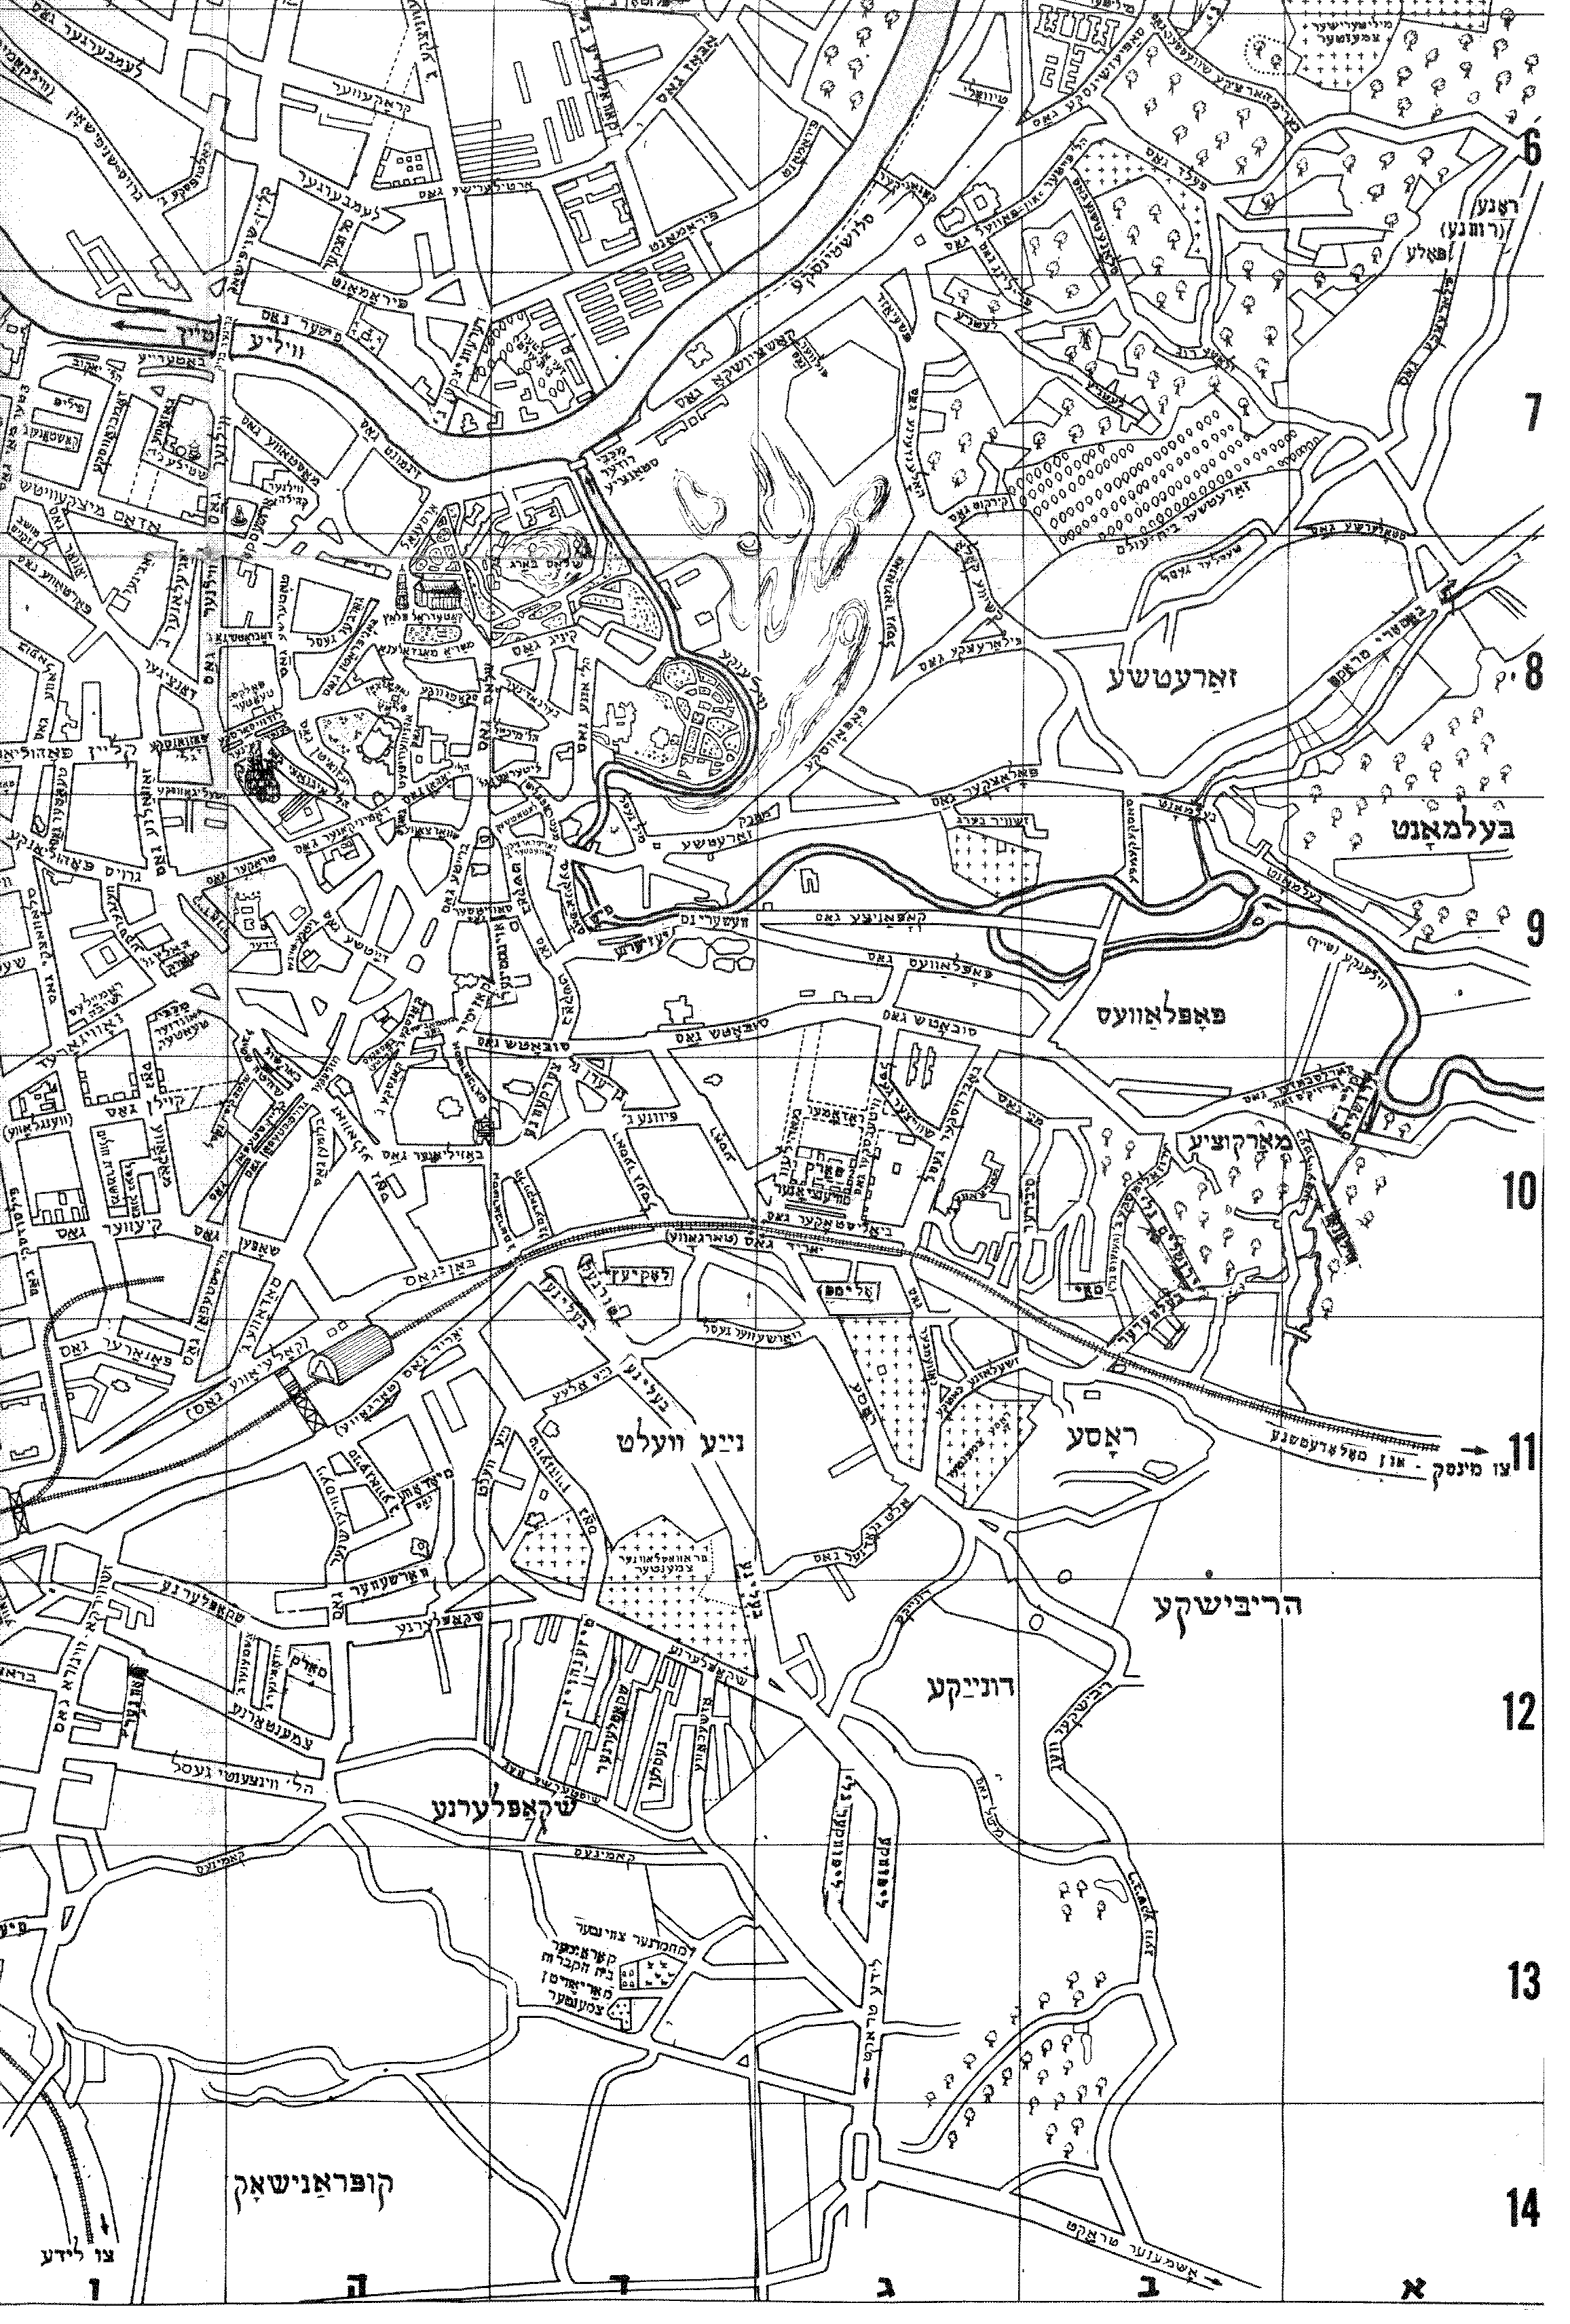
\includegraphics[width=10cm]{./ilustra-09.png} São Paulo\quad2021}
% \end{center}

\begin{figure}[!hp]
    \centering
    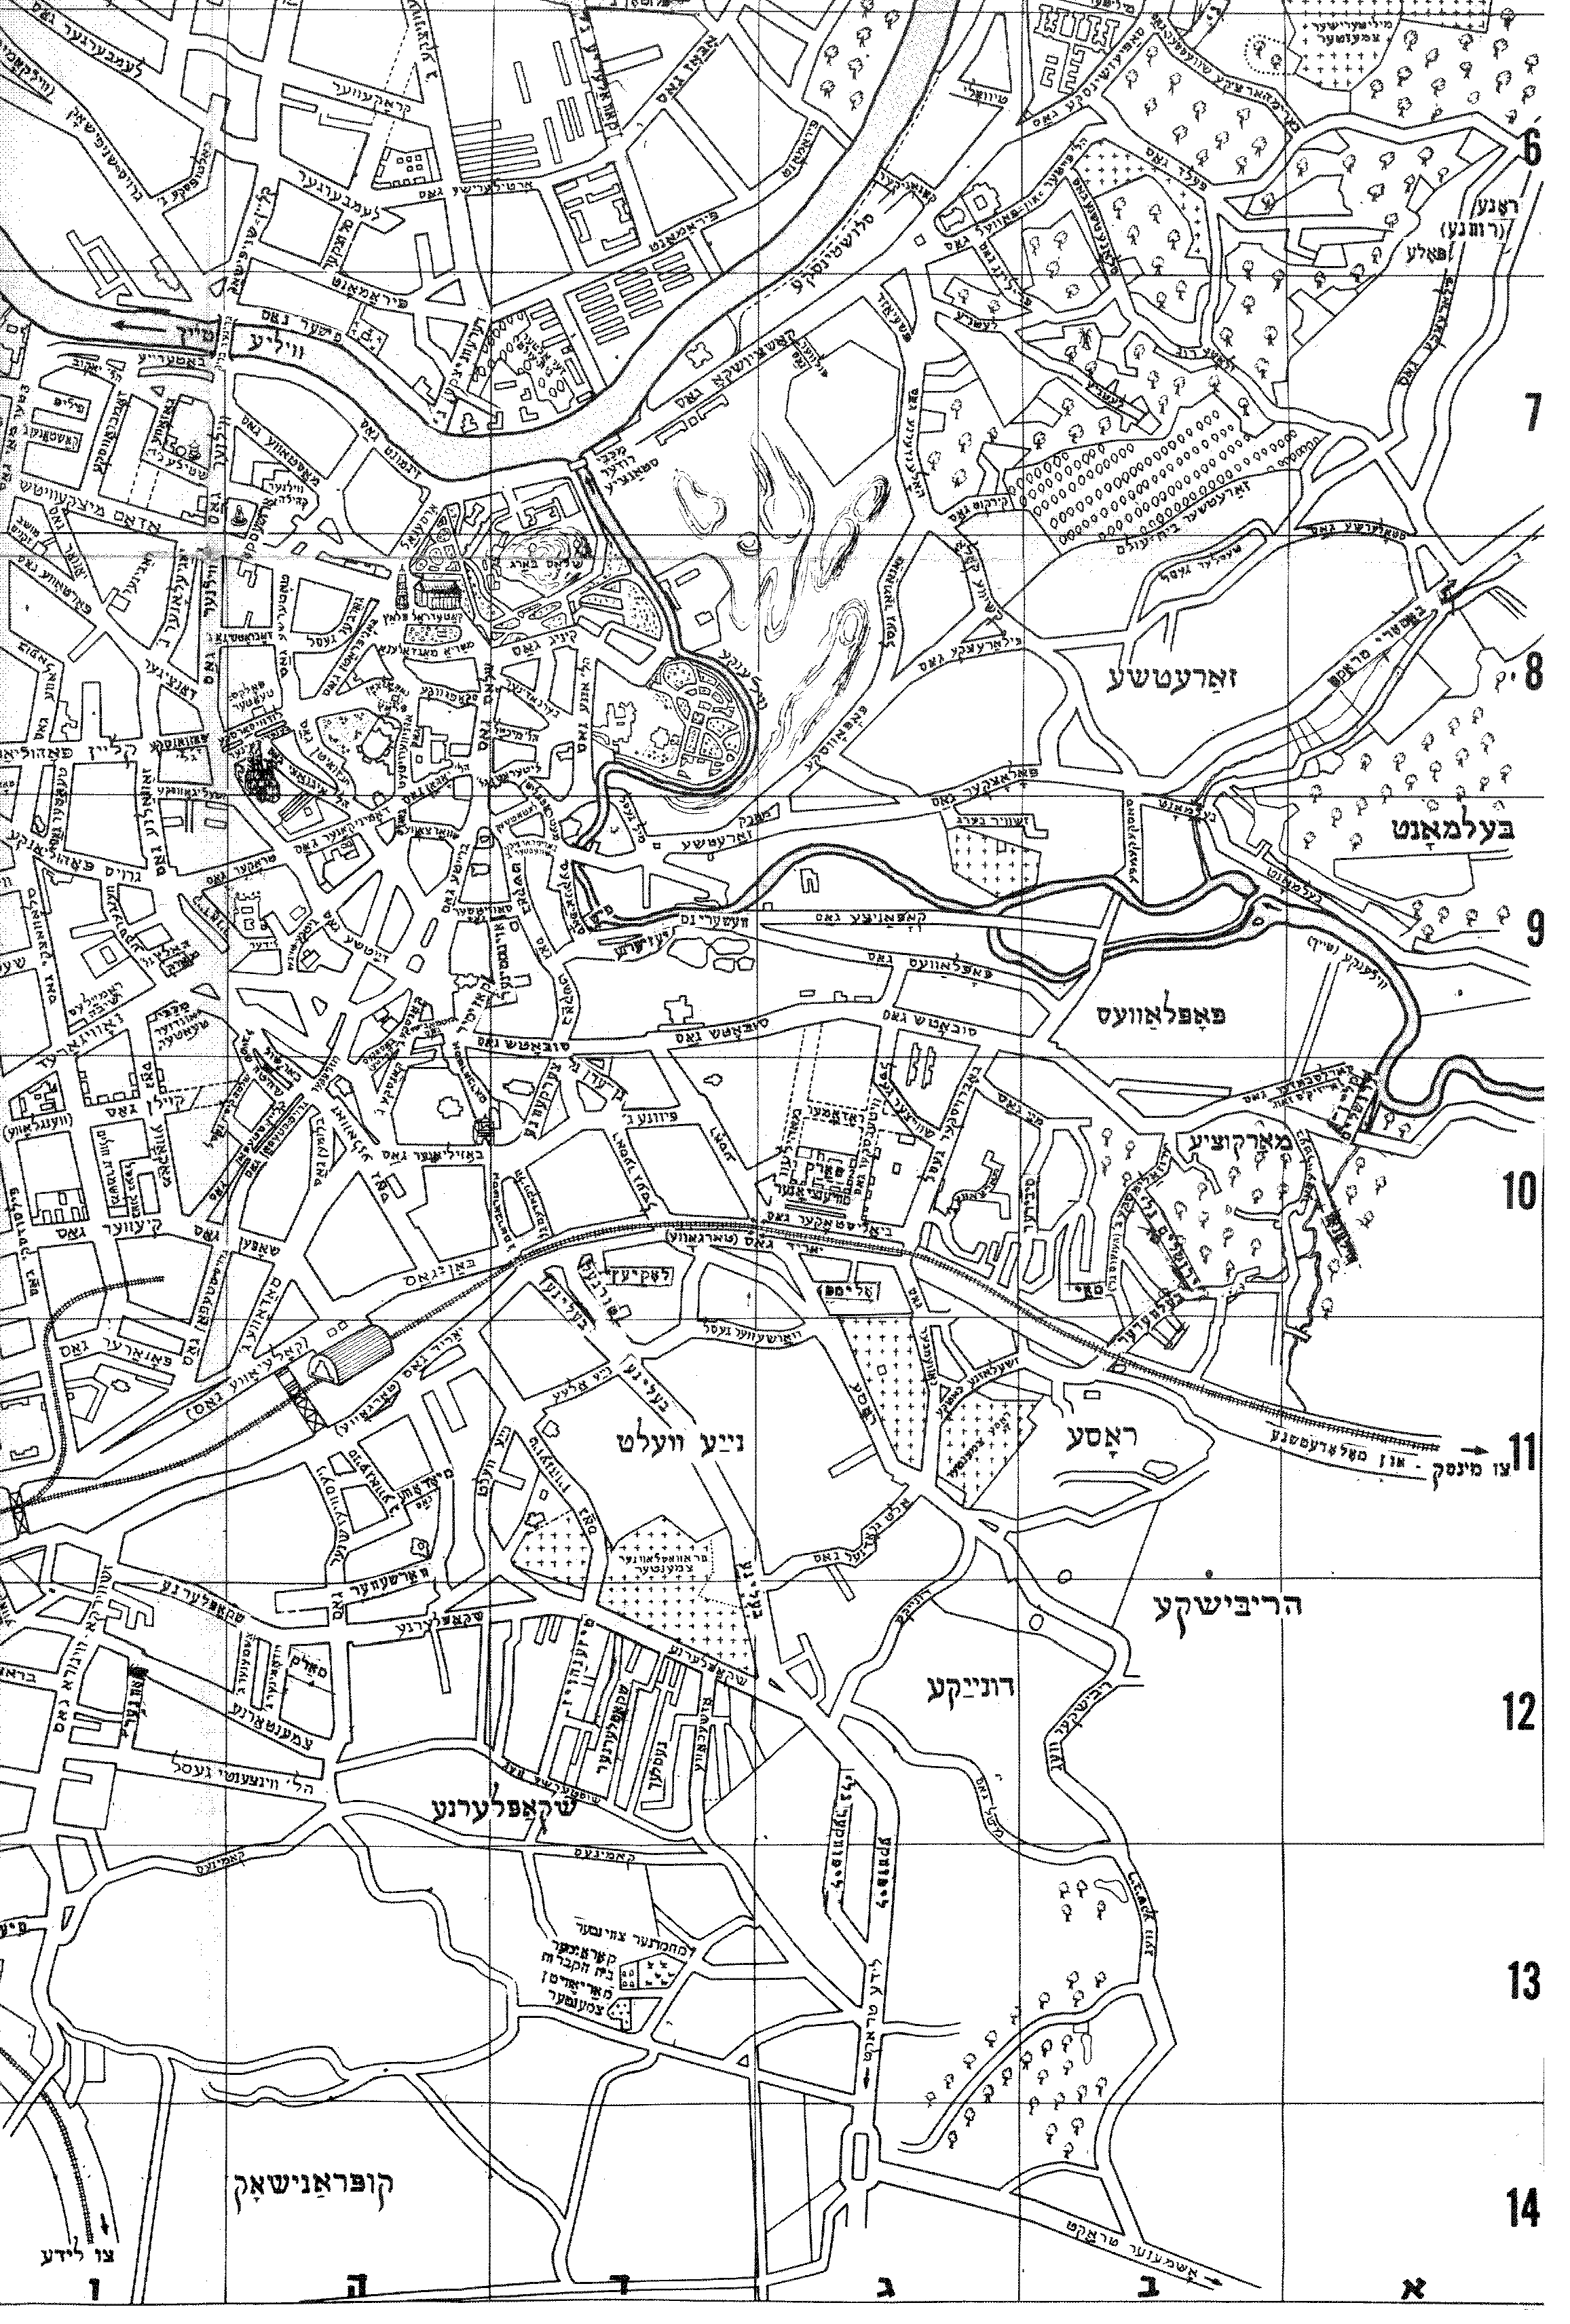
\includegraphics[width=\textwidth]{ilustra-09.png}
    \caption{Mapa de Vilna em iídiche, por volta de 1940.}
\end{figure}

Inicialmente, os passeios de Monty envolviam uma pura atividade física ---
divagações livres pela cidade, desprovidas do peso de memórias pessoais
ou de conhecimentos pré"-existentes sobre o lugar. Simultaneamente, o
intuito era o de desvelar os mistérios da cidade. Ao contrário da
conquista militar, que normalmente é um ato coletivo que implica em
certo grau de planejamento, perambular é supostamente um ato individual
de conquista de uma dimensão espacial. Eksteins, contudo, nos lembra de
que, durante meados da Grande Guerra, a ``guerra se tornou cada vez mais
uma questão de força interpretativa individual,'' e o itinerário ao
redor de \textit{Wilna} proposto por Monty parece se adequar a essa
ideia.\footnote{Eksteins, op. cit., p. 212.} A cada nova viagem, nova
aventura e nova formação, a relação entre o soldado e a cidade se torna
menos anônima, e o limite entre os dois, menos nítido e preciso. O
protagonista das excursões por \textit{Wilna} acaba por considerar
progressivamente mais difícil separar a cidade ocupada de sua anônima
cidade natal alemã, melancolicamente evocada. O corpóreo e o irreal se
fundem em um caráter surreal sedutor e perigosamente hipnótico, e o
soldado viajante começa a vivenciar nervosamente a cidade, ao invés de
apenas contemplá"-la. A proximidade imediata da cidade e a exposição
prolongada a ela provocam uma eclosão emocional que conduz a uma
perigosa perfuração no mundo interior do soldado.

Numa das passagens mais autobiográficas do guia, Monty mapeia uma breve
viagem por sua sala de estar. ``Não posso identificar o itinerário desta
viagem,'' declara o escritor, ``pois o trajeto é muito curto e, ademais,
não se presta ao uso público. Preciso apenas me levantar da minha mesa e
me aproximar da janela do meu quarto, e posso ver todas as atrações de
\textit{Wilna}. Toda a cidade se situa num vale que se estende entre nossa
pequena colina particular e a Colina do Castelo. Minha janela emoldura e
simultaneamente reflete esse espaço infindo de proporções russas. Daqui,
meu olhar pode facilmente deslizar pelos telhados, frontões e torres da
cidade.''\footnote{Monty, op. cit., pp. 78--79.} Mas ao invés de examinar
as maravilhas panorâmicas dessa ``vastidão russa'', Monty se concentra
nas cenas íntimas que populam os pátios e apartamentos da cidade
exposta. Devagar, mas sempre, sua evasão \textit{voyeurista} gera uma dolorosa
auto"-descoberta. Tão logo se conquistam os quadros privados da cidade, o
autor"-viajante se vê rodeado pelo espectro brilhante do lar. Não se
trata da aparição gloriosa e extática da \textit{Vaterland} encontrada
pelo Marechal Ludendorff em Kowno, mas uma visão perturbadora e
desnorteante, um delírio que só pode levar à crise pessoal. Ao se tornar
mais familiar, a cidade inflama as emoções. O \textit{voyeur} triunfante se torna
fugitivo, vítima de sua própria curiosidade, que inesperadamente se
transforma em atração fatal. Sob um exame minucioso, \textit{Wilna} se converte
em sereia, e seus efeitos hipnotizantes sobre o soldado podem ser
comparados ao estágio final da febre tifoide --- doença que ceifou tantas
vidas no fim da Grande Guerra --- descrito por Thomas Mann como
``debilitação [\ldots{}] em sua pior forma,'' quando ``ninguém é capaz de
dizer se a mente do paciente mergulhou no vazio da noite ou se ela se
tornou estranha a seu próprio corpo e saiu para passear por sonhos
remotos, profundos e silenciosos, desprovida de sinais visíveis ou sons
audíveis. O corpo jaz em apatia total. Esse é o momento da
crise.''\footnote{Thomas Mann, \textit{Buddenbrooks: the Decline of a Family}, trad. John \textsc{e}.\,Woods. Nova York: Knopf, 1993, p. 643.} A fuga --- dose de realidade --- é a única solução para essa relação doentia entre
cidade e soldado:

\begin{quote}
Uma sensação incomum toma conta do soldado que fita do alto a cidade.
Após passar meses embrenhado na floresta, as luzes e sombras da cidade
mexem com suas memórias. Como se acometido por uma alucinação, o soldado
vê as ruas e as praças de sua cidade natal. A guerra gerou um fenômeno,
algo que se revolve entre a pátria e a terra estrangeira.

Após sobreviver a todas as estações do ano no mato --- depois de um ano na
linha de frente --- ganhamos um desejo incontrolável pela cidade. Queremos
ver ao menos casas não"-danificadas, de telhados intactos e vidraças
inteiras. Sentamo"-nos junto à janela e olhamos para essa cidade --- cujo
nome jamais quisemos saber --- e sentimos como seu ritmo rege nossa vida.
O mistério da cidade se desdobra: desconhecida mas tão querida,
estrangeira mas tão íntima, a cidade se despe diante do nosso olhar.
Estranha mas familiar, essa cidade lá embaixo fala com os nossos
sentimentos. Seu corpo de pedra se torna menos enigmático; mas sua alma,
sua voz interior, iluminada pela luz brilhante do meio"-dia, permanece em
silêncio. É só depois do escurecer que ela lentamente começa a se
aproximar. No escuro, quando o brilho das velas do \textit{shabat} nos atinge a
partir de janelas descobertas, e quando numa quente noite de verão um
suave murmúrio dos lares de seus habitantes (que, devido à guerra, estão
proibidos de sair às ruas) começa a pairar, nossos sentimentos,
seduzidos por tais segredos, se acalmam. Seria contudo muito melhor se
nossas emoções pudessem permanecer intactas, de modo a podermos
abandonar todos esses murmúrios e sussurros e voltar ilesos para a
escuridão da noite.\footnote{Monty, op. cit., pp. 79--82.}
\end{quote}

Tal ligação sentimental e torturadamente estrangeira por \textit{Wilna} --- uma
raridade na época --- teria de ser contrastada com a relação mais prosaica
entre a cidade e seus ocupantes alemães, os quais, em algumas ocasiões,
se comportaram de maneira intensa dos pontos de vista físico e
emocional, assim como as oníricas invasões urbanas sugeridas por Monty.
\textit{Wilna}, como qualquer outra cidade do fronte, tinha casas de tolerância
e, para muitos soldados alemães, seus breves encontros continham óbvios
aspectos sexuais. Nesse caso, a relação entre os dois ``parceiros'' era
mantida em memórias particulares e pessoais, posto que o exército alemão
e a censura social não permitiam que a discussão de tais assuntos
chegasse ao público na \textit{Vaterland}. É difícil avaliar a extensão
dessas relações socialmente assimétricas, mas parte da interação entre
as mulheres do lugar e os soldados alemães se baseou mais numa
co"-dependência uniforme quanto aos aspectos social e material. Por
exemplo, Lucien Finance, um alsaciano que servia o exército alemão em
\textit{Wilna}, se casou com uma local. Suas reminiscências da cidade
(registradas em 1995!) indicam um grau razoável de reciprocidade entre
as moradoras polonesas e os soldados alemães. Os comandantes militares
alemães, aliás, não tinham confiança nos latinizados ``homens da
Alsácia"-Lorena\ldots{} portanto eles eram, em geral, enviados para o
Leste.''\footnote{Ludendorff, \textit{My War Memories}, vol. 1, op. cit., p. 137.} Assim, vários alsacianos ``não"-confiáveis'' ficaram estacionados em \textit{Wilna} e arredores, e talvez só esse fator baste, como
Finance sugeriu, para explicar o maior grau de sociabilidade dos
soldados alemães para com a população local. No final das contas, os
alsacianos, assim como a maioria dos habitantes da cidade, possuíam uma
identidade de fronteira: a maior parte deles era bilíngue e sua lealdade
nacional dependia sempre da sorte imperial e dinástica de forças
europeias contrárias.

%{[}figura 61{]}
%
%\textit{Wilna} no quarto ano da Grande Guerra, 1917.

Enquanto realizava uma viagem particular por Berlim e Königsberg,
Finance, oriundo da pequena cidade alsaciana de Seleste, foi
involuntariamente levado para \textit{Wilna}. Ali vivenciou sua primeira batalha
feroz, durante a qual, conforme evocou décadas mais tarde, ele
``provavelmente cometera coisas terríveis.'' ``Alguém tinha de morrer,''
narra Finance, ``e eram eles {[}os russos{]} ou eu.'' Após a ``defesa
heroica'' da Ponte Verde de \textit{Wilna}, o comandante de Finance quis
indicá"-lo para a Cruz de Ferro. Mas ele ligava menos para a vaidade
militar do que para a sobrevivência pessoal: ``Disse"-lhe que não
precisava da Cruz de Ferro. Ao invés disso, pedi"-lhe que me ajudasse a
me manter longe do fronte. O comandante prometeu empregar"-me em seu
escritório, pois, conforme explicou, `um homem tão corajoso merece o
nosso respeito!' Por conseguinte, o capitão me colocou no setor de
contabilidade do quartel"-general militar.''\footnote{Jean"-Noel Grandhomme, ``Vilnius 1915--1918 m. seno kareivio iš Elzaso prisiminimai'' em \textit{Metai}, julho de 2000, p. 130.} Devido ao fato de sua coragem ter sido notada, desde o primeiro dia da ocupação alemã
de \textit{Wilna} até a retirada final das tropas alemãs em novembro de 1918,
Lucien Finance morou na cidade.

Ele logo se apaixonou por Maria, uma polonesa que trabalhava no banco
local e, ao término da estada em \textit{Wilna}, eles se casaram. (Depois da
guerra, Maria se mudou com ele para a França.) De modo que, nas
recordações de Finance, \textit{Wilna} emerge como um lugar onde acontecimentos
antes ordinários da vida familiar, mesmo que incomuns, se entrelaçam com
a vivência quotidiana da linha de frente: batalhas, ferimentos, mortes
súbitas, doença, fome, saque, disciplina, subordinação hierárquica,
deserção e assim por diante. Portanto, em suas memórias distantes,
detalhes pessoais triviais e experiências íntimas da cidade prevalecem
sobre experiências panorâmicas ou heroicas do lugar. Em resumo, para
Lucien Finance, como talvez para vários outros soldados alemães, \textit{Wilna}
não exprimia nenhum significado diretamente ideológico ou claramente
geopolítico. Era simplesmente, como relatou, um local familiar do
``outro lado da Europa'', para onde foi levado pelas imprevisíveis
forças da guerra imperialista.\footnote{Ibid., p. 136.}

%{[}figura 62{]}
%
%Mapa alemão da Polônia e Lituânia, delineando as fronteiras instáveis
%dos novos estados, ca. 1923.

\chapter{Nação ausente}

%\setlength{\epigraphwidth}{.45\textwidth}
\begin{epigraphs} 
\qitem{Não é de todo fácil que um estrangeiro consiga compreender o conflito
ocorrido pouco tempo atrás entre a Polônia e a Lituânia no que toca à
bela cidade de \textit{Wilno}. Se for afeito aos livros de história, ele
recordará que \textit{Wilno} já foi a capital do Grão"-Ducado da Lituânia e que,
em tempos passados, os grão"-duques da Lituânia eram ao mesmo tempo reis
da Polônia. [\ldots{}] Em poucas palavras, parece pairar um mistério nessa
tal cidade de \textit{Wilno}, onde ora todos são lituanos, ora ninguém.}{``Algumas aparências desconcertantes'' em \textit{A estória de Wilno}}
\end{epigraphs}

Na parte oriental da Europa, a paz chegou devagar. A assinatura do
armistício no Fronte Ocidental, em novembro de 1918, que exigia a
retirada alemã de todos os territórios ocupados, só fez alimentar a
condição fronteiriça de Vilna. No vasto território deixado pelas forças
alemãs --- do Báltico ao Mar Negro --- uma série de estados nascentes
tentavam plasmar sua existência política a partir dos despojos da Europa
imperial. A Rússia, agora radicalmente transformada pela dupla revolução
de 1917 em um estado soviético e flagelado por conflitos civis, terror e
fome, estava ávida porém incapaz por restabelecer sua dominação
pré"-guerra na região. A Alemanha imperial, agora República de Weimar, se
encontrava também politicamente fraca, militarmente contraída e
demasiado esvaziada do ponto de vista social para fazer alguma notável
diferença no rearranjo geopolítico da região, e as potências vencedoras
--- Grã"-Bretanha, França e \versal{eua} --- estavam demasiado distantes, divididas e
descompromissadas para resolver problemas locais de fragmentação
nacional e ideológica. Basicamente, o pragmatismo político se tornara a
regra do engajamento: o inimigo do inimigo era um amigo, independente da
coloração nacional, fundação ideológica ou perspectivas futuras de
aliança. No entanto, quase todos os governos, apoiados por potências
ocidentais, estavam lutando contra o avanço do exército vermelho, mas a
guerra entre os novos estados e no interior deles era tão viciosa quanto
aquela que se baseava no combate global entre comunismo e capitalismo.
No fim, com a solidificação de vários povos em estados, teorias de
internacionalismo e luta de classe foram substituídas pelo conceito de
auto"-determinação nacional. A Europa moderna estava se tornando um
continente de estados"-nações --- uma colcha de retalhos de diversos países
aglutinados por animosidades externas e desconfianças internas. Em
grande parte, essa nova Europa recobria a mesma área geográfica da há
muito esquecida região da Sarmácia, parte do continente marcada por
fluidez espacial e contradições históricas.

Impérios se erguiam como negócios de famílias reais; repúblicas, pelo
menos teoricamente, eram questões de assembleias populares. Enquanto o
futuro da nação"-estado na Europa era discutido pelos vencedores, massas
de gente deslocada pela guerra e subsequentes revoluções, fatigadas por
anos de privações e doenças (1918 foi o ano da pandemia de gripe que
ceifou milhões de vidas), tentavam encontrar um lar. Para inúmeros
europeus, a mobilidade geográfica não era questão de opção. A busca de
um lar e, em muitos casos, da família perdida, era uma tarefa árdua e
sem fim à vista. Para algumas pessoas, as mudanças constantes feitas na
cartografia política da Europa produziram um deslocamento diferente: com
o surgimento de novos estados, era fácil ir parar num país estrangeiro
sem nem mesmo mudar de casa.

Naqueles anos de tumulto geográfico, portanto, o lar era muito mais do
que pudesse indicar um mero endereço residencial (o qual, aliás, poderia
mudar da noite para o dia graças à obsessão ideológica de algum novo
regime em renomear ruas e lugares). Múltiplos deslocamentos acenderam o
desejo de viver uma identidade independente de guerras e convulsões
sociais. O lar se transformou num lugar enraizado dentro das pessoas,
num sentimento de solidariedade comunitária e companheirismo social. A
ideia de nação e novas formas de estado oferecia uma espécie de
conforto. A nação"-estado era uma resposta aos problemas herdados do
velho mundo, embora não servisse a todos de maneira equitativa ou
idêntica. Numa viagem coletiva de auto"-descobrimento, a Nova Europa
exigia a renúncia de parte significante do passado de cada um,
descartando a memória pessoal e a experiência particular como atributos
de uma era passada.

Algumas nações, como a Polônia, emergiram do turbulento processo de
criação de um estado moderno como vencedores machucados, instituindo
réplicas reduzidas da antiga ordem imperial com um território vasto e
diversificado, e uma população heterogênea e multicultural. Outras, como
a Lituânia, menos exitosas em atingir objetivos nacionais, ficaram com
orgulho ferido, redução territorial, insignificância política e
marginalização cultural. Nesse ambiente de oportunidades desiguais,
Vilna tentou fracassadamente encontrar um nicho como local de
alavancagem, um lugar onde a vida da nação não precisasse se aliar de
novo à prática do estado. Essa ideia de originalidade de Vilna no
contexto do novo mapa da Europa foi uma ilusão intelectual, defendida
por um grupo de ativistas locais que buscavam respostas aos dilemas
modernos do caduco reino do Grão"-Ducado da Lituânia. Suas explorações
filosóficas jamais se materializaram, pois, de acordo com um dos
defensores dessa ideia, o caos na cidade do pós"-guerra, acentuado por
mais uma onda de refugiados e por pressões militares externas e
ideológicas, era tão imenso que não havia aptidão social ou política
capaz de mudar alguma coisa.\footnote{Mykolas Römeris, \textit{Dienoraštis}, trad. Vaiva Grigaitienė. Vilna: Versus Aureus, 2007, p. 183.} Em essência, os princípios políticos em vigor da ocupação militar nunca abandonaram a cidade, pois mesmo depois da
partida das últimas tropas alemãs nos primeiros dias de 1919, Vilna foi
tratada por todos os lados em conflito --- os governos polonês, lituano e
soviético --- como território conquistado.

A questão nacional de Vilna, ou seja, o problema de sua pertinência
política, ameaçava o santuário diplomático da Conferência de Paz de
Paris, convocada em 1919 pelas partes vencedoras com vistas a
cartografar o futuro da Europa do pós"-guerra. A questão, contudo, era
complexa demais e, ao mesmo tempo, mundana demais para que os líderes
das grandes potências fizessem dela uma lição diplomática de
reconciliação nacional. Os lituanos reivindicaram \textit{Vilnius} como capital
histórica de direito da Lituânia independente; os poloneses rejeitaram
tal reivindicação com base nas afinidades culturais e linguísticas de
\textit{Wilno} com a Polônia. O regime soviético, em isolamento diplomático,
externou a opinião segundo a qual Vilna, embora houvesse feito parte da
Rússia, seria naturalmente compartilhada pelos bolcheviques com os povos
oprimidos (sobretudo camponeses) de origens lituana e bielorrussa. Ninguém
perguntou nem quis escutar o que \textit{Vilne} significava para os judeus.

Mas a disputa diplomática pela cidade ficou no ar, em parte porque
nenhuma das partes realmente controlava a região. Num breve período de
dois anos (1918--1920), a cidade vivenciou uma enxurrada de exércitos
ocupantes, desde o exército vermelho até legionários poloneses e
voluntários lituanos. Os habitantes locais se acostumaram à vida no
campo de batalha, e os que eram corajosos o bastante para se aventurar
fora de casa assistiam a um verdadeiro espetáculo de lutas entre as
diferentes facções beligerantes na segurança de uma colina distante. A
violência era casual mas previsível --- os bolcheviques visavam os
representantes da ``burguesia nacional''; os poloneses visavam sobretudo
comunistas e judeus, trazendo o espectro do \textit{pogrom} a cada nova ocupação.
Desprovidos de qualquer vantagem militar efetiva, as autoridades
lituanas tentavam impor a supremacia linguística governando a cidade em
lituano, idioma desconhecido à vasta maioria dos residentes.

Em 1920, a cidade se tornou capital de um principado militar renegado,
estranhamente chamado de Lituânia Central, presidido por uma legião de
oficiais poloneses insubordinados. Finalmente, em 1922, depois de um
plebiscito duvidoso (por ter sido boicotado por muitos não"-poloneses),
\textit{Wilno} foi incorporada à República da Polônia como centro de uma
província polonesa recém"-criada. Mas a questão do estatuto nacional da
cidade persistia devido à exigência lituana de devolvê"-la a seu país. De
fato, apesar de ser uma cidade provincial na Polônia, \textit{Vilnius} fora a
capital constitucional da Lituânia. Esse conceito legal manteve ambos os
países em permanente estado de guerra: a fronteira --- na verdade, a linha
do cessar"-fogo --- entre a Polônia e a Lituânia jamais foi ratificada, e
não se permitiu que nenhuma rede postal ou de transporte cruzasse essa
fronteira. A adoção polonesa da cidade nunca foi abrangente e, mesmo
duas décadas depois do fim da Grande Guerra, a contestação do seu
estatuto foi observada em \textit{The National Geographic Magazine}. Em
1938, a revista difundiu uma foto com os dizeres: ``\textit{Wilno}, filha adotiva
da fronteira polonesa.''

%{[}figura 63{]}
%
%\textit{Wilno}: Avenida São Jorge, ca. 1920.

\asterisc

O escritor alemão Alfred Döblin detestava viajar. Seu descontentamento
em sair de casa mesmo que por uma breve viagem era, sem dúvida,
acentuado pela experiência do isolamento nas trincheiras da guerra no
Fronte Ocidental; mas também considerava viajar uma intenção frívola,
adequada apenas ao burguês preguiçoso ou ao tolo entediado. Ele se
interessava, contudo, pela vida urbana, em especial por sua expressão
moderna e metropolitana. Berlim, ou, mais exatamente, o agitado bairro
da classe trabalhadora que circundava a caótica praça Alexanderplatz,
era o centro de seu universo. Ele vivia num bairro com a esposa e três
filhos, trabalhava como médico no escritório de saúde público local e,
graças à sua imaginação literária --- e seu mais célebre romance,
\textit{Berlin Alexanderplatz} --- ele tornou a praça sinônimo do
\textit{Zeitgeist} modernista. A exploração urbana, com todos os
acontecimentos imprevisíveis e trivialidades de melodrama, foi
transformada em código representacional de toda experiência
metropolitana, mas Döblin também fez dela uma forma de artesanato
político, uma crítica social à era moderna, desprovida de qualquer
nostalgia, sentimentalismo ou banalidade ideológica.

A vida da cidade corre no sangue das palavras de Döblin, delineando
padrões modernos de migração urbana. O escritor era um autêntico
berlinense e tinha a cidade como lar, embora, como vários dos habitantes
da época, não fosse um nativo. Ele nasceu em 1878 na cidade de Stettin,
no Mar Báltico, onde o pai, Max Döblin, tinha um pequeno negócio. Aos
quarenta anos, o pai abandonou a família e fugiu com a amante para
Hamburgo. Alguns anos depois, teria sido visto nos Estados Unidos.
Enquanto isso, a mãe de Döblin, pobre e abandonada, mudara"-se para
Berlim junto com os cinco filhos. Esse gesto, conforme as palavras do
escritor, determinou toda a sua ``maneira de ser.'' A mudança abrupta do
relativo conforto da provinciana Stettin para a pobreza abissal da
metropolitana Berlim o fez compreender que havia se tornado membro
permanente da ``nação que era pobre.'' Anos mais tarde, Döblin ingressou
nas fileiras da classe profissional, embora jamais tenha deixado de ser
leal aos pobres do mundo.\footnote{Alfred Döblin, \textit{Destiny's Journey}, trad. Edgar Passler. Nova York: Paragon House, 1992, p. 105.}

O escritor cresceu como alemão, mesmo que, assim como recorda em sua
autobiografia pós"-Segunda Guerra, ``tenham"-lhe contado em casa, em
Stettin, que {[}seus{]} pais tinha origem judaica.'' Os avós ainda
falavam iídiche --- mas os pais já falavam alemão, com alguma inflexão
polonesa. Döblin percebia um pouco dessa confusão cultural no pai que os
deixara, e que ele simultaneamente ``amaldiçoava em voz alta e admirava
em silêncio.''\footnote{Heinz Graben, ``Introduction'', em Alfred Döblin, \textit{Journey to Poland}, trad. Joachim Neugroschel. Nova York: Paragon House, 1991, xv.} Max Döblin era uma pessoa sem terra natal. Era, nas palavras do filho, etnologicamente ``vítima do reassentamento.
Todos os seus valores foram reavaliados e desvalorizados.''\footnote{Döblin, conforme citado em Graben, op. cit., \textsc{xv}.} Döblin ansiava por reverter esse nomadismo cultural tentando se reconciliar com o mundo perdido dos
ancestrais: ``Só na minha geração a memória, inclusive a memória alegre
de nossa origem, e o antigo respeito, foi profunda e gradualmente
revivificada.'' E se arrogou um sucesso: ``Eu --- sobrevivi ao grande
reassentamento.''\footnote{Ibid.}

Isso foi um salto substancial, pois, na infância de Döblin, a religião e
a etnia da família passaram quase despercebidas. Os pais assimilados
celebravam apenas duas festas judaicas --- o Ano Novo e o Iom Kipur --- e
aquilo ``era quase a única coisa relativa ao judaísmo que pude observar
em nossa família.'' Na escola, também, ``a instrução judaica era
duvidosa e antes voluntária. [\ldots{}] Quanto ao ensinamento, o
verdadeiro ensinamento religioso --- eu o lia e escutava. Foi, e
permaneceu, superficial para mim. Não me afetou emocionalmente. Não me
senti conectado a ele.''\footnote{Döblin, \textit{Destiny's Journey}, op. cit., pp. 105--106.}

Durante a Grande Guerra, Döblin serviu como médico no exército alemão,
ajudando a aliviar as tragédias humanas que se desdobravam nos hospitais
de campo sobrecarregados do Fronte Ocidental. Voltou das trincheiras
como pacifista convicto, anti"-nacionalista e crítico implacável dos
novos regimes políticos da Europa. Escreveu também um romance biográfico
sobre Wallenstein, um dos mais cruéis e pérfidos generais da Guerra dos
Trinta Anos. O romancista começou a se interessar mais pela política
judaica só depois, quando, na ``primeira metade da década de 1920, algo
semelhante a \textit{pogroms} passou a ocorrer em Berlim, na parte oriental da
cidade, na rua Gollnow e redondezas.'' Ao se tornar membro de um grupo
de discussão que investigava questões de anti"-semitismo, ele foi
convidado por proeminentes intelectuais sionistas alemães a participar
de uma viagem à Palestina. A proposta teve um efeito atípico sobre
Döblin: ``Para ser exato, não concordei em ir para a Palestina, mas
senti que queria descobrir mais sobre os judeus. Percebi que não os
conhecia. Não podia chamar de judeus meus conhecidos que se diziam
judeus. Eles não eram judeus na crença nem na língua, eles talvez fossem
o vestígio de um povo extinto que há muito tempo havia se assimilado ao
ambiente. Então perguntei a mim mesmo e às outras pessoas: onde estão os
judeus? A resposta foi: na Polônia.''\footnote{Ibid., p. 110.}

O escritor"-médico partiu para a Polônia no outono de 1924, representando
o \textit{Die Neue Rundschau}, revista que publicava a maioria de seus
trabalhos literários. Döblin foi incumbido de escrever uma série de
relatos sobre os mais diversos aspectos sociais, culturais e políticos
da nação"-estado polonesa moderna, que seguia sendo um corpo territorial
e nacional estranho aos olhos da maior parte dos alemães. O itinerário
da viagem de três semanas, paga pela revista, foi definido pelos
interesses pessoais e sensibilidades criativas de Döblin. Ele sabia
muito pouco sobre a Polônia, e não ardia de vontade de ler tomos de
livros acadêmicos, que suspeitava fossem tendenciosos, entediantes e
desatualizados. Em suas explorações narrativas por Berlim, ele se baseou
na técnica representacional daquilo que chamou de imaginação factual
(\textit{Tatsachenphantasie}), criando uma forma expressionista de
realidade fundada no princípio da montagem. Ele explorou e narrou a
Polônia de maneira similar. Dois anos após a viagem, Döblin publicou um
livro de título simples --- \textit{Reise in Polen} (\textit{Viagem pela
Polônia}). O livro se opunha ao crescente fluxo de publicações
anti"-polonesas e anti"-judaicas --- e ainda tinha a rara qualidade da
análise introspectiva.

Ao longo do século \textsc{xix}, os judeus europeus ocidentais assimilados não
raro olhavam para seus irmãos europeus orientais com um misto de
ressentimento e fascínio. O etnógrafo Age Meyer Benedictsen, cujo pai
fora um rico judeu dinamarquês, visitou a Lituânia na última década do
século. Ele pertencia à geração dos pais de Döblin --- ``as vítimas do
reassentamento.'' A descrição detalhada dos judeus lituanos revela um
contraditório senso de superioridade e vergonha, misturado a compaixão e
assombro, que os judeus ocidentais em geral exprimiam diante da massa de
judeus não"-assimilados do Leste europeu:

\begin{quote}
Os judeus estão presentes na Lituânia desde os primeiros registros
confiáveis, mas nenhum deles quis ou foi capaz de se assimilar aos
habitantes nativos do país. Sua presença numerosa, seus preconceitos,
seu fanatismo religioso e sua antiga legislação exclusivista tenderam a
consolidar sua posição como um elemento completamente estrangeiro no
país. Os séculos de convívio antes os distanciaram da raça nativa do que
os aproximaram dela, eles não falam a língua do país entre si, mas usam
o próprio dialeto hebraico"-alemão, não se vestem como o resto das
pessoas; embora tenham sido proibidos de usar suas roupas peculiares,
eles conseguem se vestir de maneira a se diferenciar das outras pessoas.
Não têm amigos nem inimigos, nem interesses comuns com as pessoas. A
política dos judeus tem sido sobretudo oportunista, e isso por
necessidade; jamais se dispuseram a fazer amigos verdadeiros por medo de
fazer inimigos. Eles cuidadosamente escolheram o bairro em que pudessem
contar com a maior proteção durante o tempo em que ali morassem, e
jamais ousaram confiar na ideia de estar em segurança; eles
provavelmente não teriam interesse em viver ali caso sentissem que
estivessem morando no próprio país. A Lituânia é o lugar em que os
judeus tiveram a mais simples e a mais sincera crença no Messias. Em
nenhum outro lugar eles estiveram mais preparados para receber o
Redentor do que nesse recanto fora de mão, onde as circunstâncias lhes
permitiram preservar todas as memórias, tradições e hábitos na inteireza
de sua obscuridade mística. Até o dia de hoje, os judeus lituanos, com a
mesma convicção de séculos atrás, repetem: `Ele virá seguramente e Ele
virá logo.'

Deve"-se olhar para o judeu lituano à luz dessa crença inabalável, ou em
todo caso atendo"-se às propensões hereditárias que baseiam essa crença,
a fim de tentar compreendê"-lo, pois só assim pode"-se perdoar todo o seu
estilo de vida; algo grandioso pode até ser identificado nesse povo que,
de outra maneira, involuntariamente passa uma impressão desfavorável.

Os judeus lituanos se sentem estrangeiros, meio indigentes em meio a um
povo que os evita, toda a sua existência é um desafio contínuo para
manter uma posição equilibrada da maneira mais fácil, para ganhar o pão
necessário, lutando à sua própria maneira astuciosa no intuito de obter
o máximo possível de poder, e pela concepção judaica eles não se
preocupam muito se esse poder fará bem ou mal ao país em que vivem.
Humilde e desgraçado como o judeu em geral parece ser, o orgulho da raça
ainda o habita. Por menos que se importe com a rudeza e o desdém dos
infiéis, ele só comete uma traição se for obrigado, e seu orgulho mental
não sofre com isso. [\ldots{}] Sujo, mesquinho e ganancioso de um ponto de
vista superficial, o judeu ainda possui o ouro da alma, capaz de
cintilar no momento oportuno, e quem se aproximar dele sem preconceitos
tolos poderá notar o que há de bom nele, e então as melhores qualidades
humanas, simpatia e gentileza se tornam aparentes.

Essa situação discrepante é a causa da posição falsa em que os judeus se
lamentam na Lituânia, e há muitos dentre eles que perderam o objetivo de
vista, absorvidos pelos meios de atingi"-lo.\footnote{Benedictsen, op. cit., pp. 212--214.} 
\end{quote}

Na virada do século \textsc{xx}, um número crescente de intelectuais judeus
alemães começaram a buscar suas raízes culturais ancestrais nas inúmeras
\textit{shtetlakh} da Europa Oriental. Essas descobertas etnográficas,
literárias e por vezes genealógicas eram promovidas por uma revista
influente com nome sugestivo, \textit{Ost und West}. A revista introduziu
o tema da reconciliação entre os dois ramos do judaísmo \textit{ashkenazi}: os
europeus ocidentais emancipados --- os \textit{Westjuden} --- e os europeus
orientais mais tradicionais --- os \textit{Ostjuden}. Sua política editorial
``falava repetidamente de uma identidade judaica `harmoniosa', uma
identidade que se equilibrasse entre a tradição e a modernidade, entre o
Leste e o Oeste.''\footnote{David Brenner, \textit{Marketing Identities: the Invention of Jewish Ethnicity in ``Ost und West''}. Detroit: Wayne State University Press, 1998, p. 34.} Os contatos sociais entre as duas comunidades aumentaram no período de entreguerras, quando o
exército alemão passou a controlar um vasto território russo habitado
pelos \textit{Ostjuden}. A guerra e a revista, cujo último número foi
publicado um ano antes da viagem de Döblin à Polônia, possibilitou aos
``judeus entre vinte e quarenta anos romper com o aspecto assimilativo
dos pais enquanto se distanciavam do lado negativo da
\textit{Ostjudentum}.''\footnote{Ibid., p. 83.}

A reação inicial de Döblin diante do arquétipo do ``judeu polonês'' foi
marcado por um exagerado sentimento de descrença. Em Varsóvia, no
primeiro dia da viagem, ele se viu às voltas com a própria incapacidade
perceptiva de situar a identidade judaica no contexto mutante do terreno
urbano da Europa moderna:

\begin{quote}
Estou em pé numa parada de bonde, examinando o utilíssimo diagrama do
sistema de transporte, que indica as linhas e rotas. De repente, um
homem solitário com uma barba cobrindo"-lhe o rosto se destaca da
multidão e vem na minha direção: envergando um sobretudo preto em
frangalhos, boné preto na cabeça e botas de cano alto nos pés. E logo
atrás dele, falando alto numa língua que reconheço como alemão, outro,
também de sobretudo preto, um homem enorme, com um rosto largo e
vermelho, penugem ruiva cobrindo"-lhe as faces e os lábios. [\ldots{}]
Sinto um golpe na cabeça. Desaparecem na turba. As pessoas não prestam
atenção neles. São judeus. Estou atordoado, não, apavorado.\footnote{Döblin, \textit{Journey to Poland}, op. cit., p. 7.} 
\end{quote}

Poucas horas depois da primeira visão de um judeu, a angústia
etnográfica de Döblin se metamorfoseou em fascínio cultural, e ele logo
aprendeu a observar os judeus poloneses no contexto do próprio universo.
Ele os seguia por toda parte, até que, em Cracóvia --- ao término da
viagem --- considerou a arrogância cultural e práticas sociais dos judeus
ocidentais assimilados como sendo insuportáveis e indefensáveis. ``Sei o
que os cavalheiros iluminados, os Iluminadores Judeus, dirão. Dão risada
dos membros `tolos e atrasados' de sua própria nação, têm vergonha
deles. [\ldots{}] Não sou Iluminador nem membro dessas massas nacionais,
um transeunte europeu ocidental --- vejo esses `Iluminados' como africanos
que se gabam das bolinhas de gude que receberam dos marinheiros, das
algemas sujas em seus braços dependurados, das cartolas amassadas novas
em folha sobre suas cabeças. Como é pobre, como é esfarrapado, como é
devastado pela indignidade e pela falta de alma esse Mundo Ocidental que
lhes oferece as algemas; como é que eles poderiam saber.''\footnote{Ibid., p. 191.} Contudo, típico de sua maneira solitária de ver o mundo, e sem desafiar as próprias lealdades culturais, Döblin se isolou de ambos
os tipos de identidade judaica. Escolheu o papel de observador
independente, testemunha imparcial dos dois mundos.

\asterisc

No papel, a viagem de Döblin à Polônia foi uma investigação
sócio"-política e jornalística da Polônia independente a cargo da
imprensa alemã de esquerda. O escritor tinha fortes conexões pessoais
com diversas correntes do movimento socialista, mas jamais se tornou um
ideólogo rígido ou funcionário do partido. Suas visões políticas foram
influenciadas pelo pensamento anarquista russo e ele era muito crítico
para com a função política restritiva e as práticas sociais coercitivas
do estado. Fazia também objeções à ideia de nação"-estado moderna, e foi
à Polônia para ver que ``o engano do significado único do estado e o
reconhecimento de seu poder persistem.''\footnote{Ibid., p. 240.}

A Polônia não mudou a visão negativa que Döblin tinha do estado moderno
ou da política nacionalista, embora jamais tenha se virado contra a
auto"-determinação nacional. A nação"-estado europeia, julgava Döblin,
tornou"-se automaticamente uma estrutura opressiva pois seu caráter
nacional era incapaz de abranger a heterogeneidade e diversidade locais.
A Polônia rediviva estava longe de ser um país monolítico do ponto de
vista linguístico e territorial. As estatísticas do estado, conforme
Döblin notou, não conseguiam dissimular seu caráter pós"-imperial e
multinacional: ``Estou com o Almanaque Polonês oficial de 1924; não vou
me permitir intimidar pelas estatísticas. De acordo com o recenseamento
de 1921, a Polônia atual tem uma superfície de quatrocentos mil
quilômetros quadrados, habitada por vinte e sete milhões de pessoas.
Dessas, onze milhões vieram do antigo Congresso da Polônia; oito, da
Áustria; quatro, da Prússia. Faltam quatro milhões: elas ocupam o
`território oriental', formado pelos distritos de Grodno, \textit{Wilno}, Minsk e
Volínia.''\footnote{Ibid., p. 9.} Cerca de dois terços da população eram
poloneses, quatorze por cento ucranianos, quase dez por cento eram
judeus, mais de cinco por cento eram bielorrussos, cerca de dois e meio
por cento eram alemães, e menos de meio por cento era lituano. Döblin
quis explorar o estado polonês recém"-reconstituído pelo prisma de sua
sociedade polimorfa. Logo se viu perplexo diante da tarefa. ``Em breve
vou jogar a toalha,'' anunciou o escritor, ``pois não falo a língua, ou
melhor, as línguas do país: polonês, ucraniano, bielorrusso, iídiche e
lituano.''\footnote{Ibid., p. 31.}

%{[}figura 64{]}
%
%\textit{Wilno} lê em várias línguas.

Desestimulado pela própria insuficiência linguística, o escritor se
tornou atento leitor da paisagem. O nascimento da nação"-estado polonesa
se deu sob o signo da guerra e, ao longo da viagem, ele repetidamente se
viu diante de diversas marcas topográficas do conflito pregresso:
ruínas, cidades despopuladas, desfiles de veteranos, cemitérios
militares etc. Mas sua investigação foi também conduzida pelo espectro
de guerras futuras: o ódio encontrado entre vários grupos étnicos na
Polônia, a desconfiança política dos países vizinhos, a manipulação
ideológica das massas, o isolacionismo cultural e, acima de tudo, a
veneração internacional pelo militarismo. No meio da viagem, ele cunhou
seu lema político: ``Os estados de hoje são os túmulos das
nações.''\footnote{Ibid., p. 151.}

Aflito com as descobertas sociais, Döblin --- naquela altura ateu
auto"-declarado --- buscou os universos religiosos da Polônia
multicultural. Ficou hipnotizado por cada local sagrado e visão
espiritual: espetáculos católicos exuberantes, cerimônias ortodoxas
russas misteriosas, e adoração hassídica intimista. Nesse caleidoscópio
de pluralidade espiritual frequentemente antagonista, Döblin cartografou
a direção da viagem: ``Será um mundo morto ou um mundo novo? Não sei
qual está morto. O velho não está morto. Sinto"-me íntima e violentamente
atraído por ele. E sei que minha bússola é confiável. Ela nunca aponta
para algo que seja estético, ela sempre aponta para coisas vivas e
urgentes.''\footnote{Ibid., p. 187.} Devagar mas sempre, a viagem
assumiu a forma de uma peregrinação pessoal.

Döblin deixa a agitada Varsóvia no início dos oito dias do festival de
Sucot, a Festa dos Tabernáculos. Essa antiga (e, para o escritor,
desconhecida) festa judaica transfere as tradições nômades de um povo do
deserto para a topografia movimentada da cidade moderna. A vívida fusão
de Leste e Oeste, velho e novo, secular e espiritual o diverte --- e
revela a compatibilidade dos dois mundos:

\begin{quote}
A Festa dos Tabernáculos está acontecendo logo ali na esquina. Tábuas já
estão sendo levadas para os pátios das ruas dos judeus, placas simples,
brutas, a serem marteladas e desbastadas na forma desejada. Uma porta é
inserida; o teto é coberto por plantas. Em cada pátio crescem cabanas
uma a uma. Cada família tem uma mesa com bancos, que eles colocam para
dentro. Em vários desses pátios, eles puxam um fio do sistema elétrico
até o teto do tabernáculo, para iluminar o interior. [\ldots{}] Agora vão
festejar uma festa da natureza nos pátios escuros da metrópole, ao lado
de latas de lixo, em terraços na altura dos telhados. Parece"-se com um
gesto de indestrutibilidade das massas: apesar de tudo!\footnote{Ibid., pp. 70--71.} 
\end{quote}

Após uma viagem noturna num vagão dormitório compartilhado, Döblin chega
às pitorescas cercanias de \textit{Wilno}. Ele não tem nenhum conhecimento prévio
da cidade e, emudecido pela incapacidade de conversar em qualquer um dos
idiomas locais, é incapaz de obter informações claras sobre ela dos seus
companheiros de viagem. Mas a paisagem em movimento põe a cidade no
mapa. Da proximidade incômoda do trem sonolento, \textit{Wilno} inesperadamente
surge como um lugar sedutor:

\begin{quote}
No início do amanhecer, comecei a olhar pela janela do trem. Fui
interrompido apenas uma vez, quando meu companheiro brutamontes que
dormia acima de mim colocou para fora da cama suas pernas gordas
envoltas em meias compridas de lã cheias de furos e, gemendo, calçou as
botas enlameadas bem diante da minha cara. Às sete da manhã, a paisagem
muda. Torna"-se colinosa, ondulante. Até então, ela se esticava
homogênea, como uma estepe, às vezes com um prado ou uma fazenda. Agora
se torna ondulante, colinosa. Bosques, abetos e florestas caducas são
recorrentes. Um edifício parecido com um castelo passa rápido do lado
esquerdo, uma ruína. As entradas e saídas dos túneis são vigiadas por
sentinelas com rifles; o país se encontra em estado de inquietação. Os
jornais relatam ataques dos bolcheviques e quadrilhas anônimas;
pressinto de repente que sejam mais que ataques perpetrados por
quadrilhas, e sim verdadeiras movimentações de guerra. Arrastamo"-nos
vagarosamente por uma ponte alta e estreita. Como é maravilhosamente
vívida a paisagem. As colinas se transformam em montanhas. O vermelho e
o amarelo das árvores que fenecem; entre elas, o verde escuro esfumaçado
dos abetos altivos. Fileiras compridas de vagões ferroviários nos
trilhos, agitação dentro do trem. Do lado de fora, casinhas, indivíduos,
grupos, nas ruas. Estação de \textit{Wilno}.\footnote{Ibid., p. 84.}
\end{quote}

Ainda com as memórias frescas da frenética vida das ruas da
metropolitana Varsóvia, Döblin sai para passear. Ao redor da estação
ferroviária sonolenta e provinciana, \textit{Wilno} parece trivial. As ruas sem
direção parecem levar a lugar nenhum até que, após dobrar umas poucas
esquinas, Döblin, à deriva, encontra por acaso um portão muito antigo:

\begin{quote}
Na manhã gelada, passeio ao longo da avenida. Margeada por casas baixas,
a maior parte delas velha e miserável. Então, do lado esquerdo, uma rua
leva a uma avenida, uma rua meio estreita desprovida de uma verdadeira
calçada. Continuo procurando a via principal, imaginando que haja uma.
Então o arco de um portão de entrada, alto e considerável, avulta por
cima da rua; enquanto ouço cantarem, passo pela velha estrutura,
examinando"-a. Uma multidão está agachada do lado direito: camponeses,
gente da cidade, homens e mulheres, no chão, ajoelhados, curvando a
cabeça até embaixo. Mas não são eles que cantam, o canto vem de outro
lugar, de cima. E, ao me virar, vejo lá em cima uma capela em cima do
arco. E lá, aberta para o lado da rua, um altar, com várias velas acesas
e um emaranhado de coisas que não consigo distinguir. As pessoas que
passam pela rua seguram os chapéus ou bonés na mão. Também tirei o
chapéu por debaixo do arco. Uma efígie milagrosa da mãe de Deus está lá.
A Madonna parece viva. Assoma por cima de uma tremenda meia"-lua, que se
assemelha a um enorme chifre curvo de animal. É visível do peito para
cima. Suas roupas sacerdotais são ricamente adornadas. A cabeça coroada
se inclina para a direita. As mãos cruzadas sobre o peito. O pescoço
estreito emerge das vestes e mantos esplêndidos e coloridíssimos. Então
surge uma face estreita e comprida, os olhos abertos como frestas, os
lábios fechados. Raios dourados afiados contornam toda a cabeça. Está
orando, ou em transe, ou está ouvindo suave e melancólica, ou absorvida
em sua tristeza, tentando transcendê"-la: não consigo definir sua
expressão. A imagem parece insinuante, tocada. Os fiéis aqui tendem a
fundir sua dor com a da criatura celestial para então se retirar mais
sossegados. É uma grande realização artística que uma tal imagem pudesse
ter sido feita e que uma imagem pintada possa servir de
exemplo.\footnote{Ibid., pp. 84--85.}
\end{quote}

Enquanto o encontro de Döblin com a Ostra Brama foi acidental, sua
iniciação à fé católica foi um longo processo, que culminou em 1941 com
a conversão ao catolicismo. Naquela altura, Döblin estava exilado na
Califórnia com a família; a conversão significou uma ruptura, não só com
a afiliação comunista e ateísta do escritor, como também com sua herança
judaica. Döblin menciona o caminho tortuoso mas resoluto rumo ao
catolicismo como uma sequência de revelações não relacionadas entre si:
``Há dois tipos de encontro pelos quais devemos ser gratos. Um é o
encontro com pessoas que realizam nossos desejos e respondem nossas
perguntas. O outro é o encontro com pessoas, ou livros, ou
acontecimentos ou imagens, que provocam em nós desejos e incitam em nós
perguntas.''\footnote{Döblin, \textit{Destiny's Journey}, op. cit., p. 109.} Os efeitos perceptivos de tais encontros são invisíveis, ou seja, ocorrem de maneira impremeditada e insondável, assim como alguém
volta ``para a própria casa do seu próprio jeito: desapercebido,
simples.''\footnote{Ibid., p. 322.}

%{[}figura 65{]}
%
%O portão Ostra Brama; fotografia de J. Bułhak.

O papel de \textit{Wilno} na conversão de Döblin só pode ser especulativo. Mas
talvez seja possível traçar um paralelo entre seu encontro com a cidade
e o de outro famoso converso católico, o proeminente escritor inglês
Gilbert Keith Chesterton (1874--1936). Chesterton foi ostensivamente
batizado em público em 1922, e visitou \textit{Wilno} com a esposa em 1927,
durante um suntuoso e bem planejado passeio pela Polônia. A conversão
aproximara Chesterton dos ambientes político e cultural das
recém"-surgidas nações"-estado católicas. Portanto, ao contrário de
Döblin, Chesterton foi oficialmente convidado a visitar a Polônia como
campeão proeminente dos interesses poloneses. O casal Chesterton recebeu
boas"-vindas grandiosas: na estação ferroviária de Varsóvia, foram
cumprimentados por um grande grupo de autoridades polonesas, inclusive
vários oficiais de cavalaria que representavam o Marechal Piłsudski.

Durante a viagem, Chesterton expressou seu entusiasmo irrestrito pela
Polônia. No livro de ouro do \versal{pen} Club polonês, deixou uma nota
lisonjeira: ``Se a Polônia não houvesse renascido, todas as nações
cristãs teriam morrido.''\footnote{Gilbert Keith Chesterton, conforme citado em Michael Ffinch, \textit{G.\,K. Chesterton}. Londres: Weidenfeld and Nicholson, 1986, p. 312.} Elogiou também Piłsudski, que descreveu como sendo ``muito simpático para com a Lituânia; embora lituanos e
poloneses estivessem brigando naquela altura. Nutria grande entusiasmo
por \textit{Wilno}; e mais tarde encontrei, na fronteira, um monumento histórico
em que poloneses e lituanos são vistos em paz --- mesmo quando estão em
guerra.''\footnote{Gilbert Keith Chesterton, \textit{Autobiography}. Londres: Hutchinson and Company, 1936, p. 317.} Döblin, ao contrário, descrevera Piłsudski como um personagem muito mais ambíguo: ``um
revolucionário ao estilo de Mazzini\ldots{} anti"-clerical\ldots{}
esquerdista radical\ldots{} {[}que{]} resolutamente organizou o exército
à sua própria maneira\ldots{} homem fascinante e profundamente
apaixonado, um completo anti"-parlamentar.''\footnote{Döblin, \textit{Journey to Poland}, op. cit., p. 33.}

Chesterton se deixou claramente seduzir por \textit{Wilno}, barroca ``cidade da
concórdia'' na região \textit{Kresy} (fronteiriça) da Polônia. Alguns anos
após a viagem, numa estória autobiográfica, ele transformou a cidade no
ponto alto da excursão polonesa. Como era de se esperar, o escritor não
observou ou preferiu ignorar todos os sinais de animosidade nacional. Na
sua memória, \textit{Wilno} permaneceu como localidade lúdica e inocente:

\begin{quote}
Estava guiando na companhia de uma senhora polonesa, muito espirituosa e
conhecedora de todo o caráter da Europa, e também da Inglaterra (segundo
o bárbaro hábito dos eslavos); e só percebi uma mudança no seu tom, como
uma espécie de frieza, quando paramos diante uma passagem sob um arco
que dava acesso a uma rua lateral, e ela disse: ``Não podemos passar de
carro por aqui.'' Surpreendi"-me, pois a passagem era larga e a rua,
aparentemente livre. Enquanto caminhávamos por sob o arco, ela me disse,
no mesmo tom desbotado: ``Tire o chapéu aqui.'' E então pude ver a rua
toda. Estava tomada por uma multidão imensa, todos virados para mim; e
todos ajoelhados no chão. Era como se alguém estivesse chegando atrás de
mim; ou como se algum estranho pássaro girasse por cima da minha cabeça.
Olhei para trás e vi, no meio do arco, grandes janelas abertas, que
revelavam um câmara cheia de cores e dourados; havia uma imagem por
detrás; mas partes da imagem se moviam como num teatro de bonecos,
atiçando estranhas memórias duplas como o sonho da ponte no teatro de
bonecos da minha infância; e então percebi que, a partir daqueles grupos
em movimento, brilhava e ressoava a ancestral magnificência da
Missa.\footnote{Chesterton, \textit{Autobiography}, op. cit., pp. 317--318.}
\end{quote}

Enfeitiçado pela magia do lugar e pela agradável companhia, a
curiosidade de Chesterton (ou sua memória) não se aventurou para além do
portão. Döblin, por outro lado, demonstra interesse maior pela vida
quotidiana da cidade. Desorientado mas não menos encantado, ele penetra
mais fundo na cidade, até tropeçar em mais um dos mistérios locais:

\begin{quote}
A rua se chama Ostra"-brama. Ela se estende quase silenciosa, os
adoradores mal emitem sons. Na esquina, uma equipe está enterrando canos
de esgoto no chão. Subo lentamente a rua com suas casinhas e seu
lamentável pavimento. São dez da manhã. Mas as lojas ainda estão
fechadas. Umas poucas abertas. E então olho para os nomes nas placas e
percebo que são as lojas dos judeus que não abrem. A Festa dos
Tabernáculos ainda está acontecendo.

A rua se alarga como uma praça. Do outro lado, uma velha caixa de pedra:
é o antigo teatro, com carruagens defronte. Ao passar por um cinema,
percebo que os cartazes estão em duas línguas: polonês e iídiche. As
placas de diversas lojas estão também no alfabeto hebraico, em iídiche.
Encontrei isso com frequência em Varsóvia, no bairro Nalewki; mas, aqui,
está espalhado pela cidade. Parece haver aqui uma população judaica
muito grande ou muito corajosa. Não vejo contudo nenhum judeu, e essa é
a segunda coisa. Alguns judeus devem estar andando por aí, mesmo sendo
feriado para eles. E agora noto que na verdade os vejo mas não os
percebo. Estão em pé ao meu lado do lado de fora do cinema, caminhando
de bonés brancos, jovens rapazes e moças; os mais velhos cruzam devagar
a praça esburacada, conversando na própria língua. Nenhum deles usa um
cafetã! Não vejo ninguém de ``capote'' preto. Todos se vestem com roupas
europeias --- mas sem falar polonês. É um tipo de judeu diferente dos de
Varsóvia.\footnote{Döblin, \textit{Journey to Poland}, op. cit., p. 86.}
\end{quote}

Döblin se confronta, mais uma vez, com a própria incapacidade de situar
os judeus no ambiente em que vivem. Só dessa vez, sua inaptidão é ainda
mais embaraçosa. Se em Varsóvia ele ficara superestimulado pela
imaginação excessiva, em \textit{Wilno} a falta dela o cega. Rapidamente, Döblin
compreende que, a fim de enxergar o universo judaico de \textit{Vilne}/\,\textit{Wilno} em
sua plenitude, é necessário adentrar no terreno não"-cartografado da
cultura iídiche.

\asterisc

Haim Sloves (1905--1988), escritor e dramaturgo iídiche, descreve a
paisagem cultural do iídiche --- a Iidichelândia --- como um território
permanentemente marcado pela fluidez geográfica: ``Existe um país que
não figura em mapa nenhum do mundo, um país estranho e desconhecido de
uma imensidão quase irreal, cujas fronteiras sempre inconstantes
atravessam continentes e oceanos. Trata"-se da terra do iídiche. Quantas
pessoas reivindicam para si essa língua, de Nova York a Moscou, de
Buenos Aires a Varsóvia, de Jerusalém a Paris, de Melbourne a
Johannesburgo? Milhões.''\footnote{Haim Sloves, conforme citado em Henri Minczeles, ``A journey into the heart of Yiddishland'' em \textit{Yiddishland}. Corte Madera, California: Gingko Press, 1999, p. 7.} Devido a sua natureza plural, a Iidichelândia não tinha um centro. Contudo, observadores
judeus contemporâneos ``costumavam ver Vilna como exemplar da comunidade
judaica do Leste europeu, lugar em que as ricas tradições do passado
poderiam servir como base para uma nova cultura inovadora. Assim como
disse em 1930 um palestrante durante a conferência da \versal{yivo} {[}Instituto
Científico Iídiche{]}: `para nós, Vilna não é simplesmente uma cidade, é
uma ideia.'"\footnote{Cecile \textsc{e}.\,Kuznitz, ``On the Jewish Street: Yiddish culture and the urban landscape of interwar Vilna'' em \textit{Yiddish Language and Culture: Then and Now}. Creighton: Creighton University Press, 1998, p. 66.}

O estatuto de \textit{Vilne} como eixo cultural ideal para a Iidichelândia se
fundamentava na localização geopolítica e linguisticamente indefinida da
cidade no contexto do mapa europeu fragmentado das nações"-estado. Posto
que nem uma única força nacional, linguística, religiosa ou ideológica
era capaz de governar incontestavelmente a cidade, os judeus falantes de
iídiche puderam plasmar sua própria cartografia urbana, que sobreviveu à
maior parte dos regimes reinantes:

\begin{quote}
De fato, se Vilna tinha uma geografia especificamente judaica, ela fora
em grande parte criada pelo uso de um determinado idioma. Enquanto o
nome da cidade oficialmente mudava de Vilna para \textit{Wilno} e depois para
Vilnius, os judeus a chamavam sempre de \textit{Yerushalayim d'lite}
{[}Jerusalém da Lituânia{]}, nome que jamais constou de nenhum mapa
oficial. Ademais, os habitantes judeus empregavam a língua iídiche para
pleitear sua reivindicação por determinadas partes da cidade, tanto
formal como informalmente. Assim como os judeus tinham o próprio nome
para Vilna, determinadas áreas da cidade, em particular aquelas
localizadas no bairro judaico, tinham denominações distintivamente
iídiches. A maior parte dos edifícios se organizavam em torno de pátios
{[}\textit{hoyfn}{]} que eram chamados de acordo com o nome de seus
proprietários; por exemplo, o pátio da rua Yidishe número 7 era
conhecido como Hoyfn Reb Shaul Shiske, e o da rua Yatkever número 8,
como Hoyfn Urel"-Feygl. Algumas ruas tinham também seus próprios nomes em
iídiche, como a rua São Nicolau, conhecida pelos residentes judeus como
Gitkes"-toybes zavulek {[}Alameda do Gitke"-Toybe{]}. Visto que a
designação dos logradouros mudava frequentemente devido à sucessão de
regimes --- russo, alemão, lituano, polonês --- que chegavam ao poder, os
nomes judaicos das ruas eram por vezes mais velhos e mais conhecidos do
que suas contrapartidas oficiais.\footnote{Ibid., p. 67.}
\end{quote}

Entretanto, poucos visitantes não"-judeus, ou mesmo habitantes locais,
tinham interesse pela topografia judaica da cidade. Em Varsóvia, um
``político polonês nacionalista, muito inteligente e muito pragmático''
preveniu Döblin quanto aos ``enérgicos, astutos e odiosos \textit{litvaks}'', 
judeus lituanos, que identificava como sendo a principal causa do
anti"-semitismo polonês.\footnote{Döblin, \textit{Journey to Poland}, op. cit., p. 37.} Muitos daqueles que passaram por \textit{Wilno} ficavam com uma sensação palpável de intolerância racial e religiosa. Em 1938, por
exemplo, Robert McBride, católico americano, foi ciceroneado pela cidade
por um padre polonês ultra"-nacionalista, que era também capelão militar.
Seu itinerário e, por conseguinte, suas impressões da cidade traem um
desprezo por tudo que fosse judaico:

\begin{quote}
Em cada cidade polonesa, exceto as do extremo oeste, o gueto é parte
integrante da comunidade. Em \textit{Wilno}, ele é mais proporcionadamente uma
entidade do que em qualquer outra cidade importante. Aqui, quarenta por
cento da população é judaica e, aqui, como em qualquer outro lugar, eles
preferem a reclusão e o caráter racial exclusivo do gueto à vida fora
dele. Nos atuais tempos modernos, nenhuma tentativa foi feita contra a
segregação; os judeus preferem viver amontoados em seus próprios
bairros, assim como vestem suas próprias roupas ortodoxas pretas e
mantêm as faces barbudas. Seu caráter racial e ortodoxia são
cuidadosamente guardados, e eles não gozam de nenhuma relação social com
os vizinhos poloneses. Aparentemente inassimiláveis, caso mantenham os
costumes atuais, eles permanecerão uma raça à parte e serão vistos pelos
poloneses como elemento estrangeiro na comunidade. Por que desejam
continuar segregados nas ruas estreitas e fedorentas de seus guetos é
difícil compreender. Decerto são influenciados por considerações
econômicas, de conveniência e de hábito que têm origem na época em que
se viram obrigados a viver separados dos vizinhos cristãos. A população
hebraica de \textit{Wilno} se dedica a todas as atividades comerciais --- lojistas,
mascates nos mercados, carroceiros e não duvido também que lavem as
roupas uns dos outros.\footnote{Robert Medill McBride, \textit{Towns and People of Modern Poland}. Nova York: McBride and Company, 1938, pp. 137--138.} 
\end{quote}

%{[}figura 66{]}
%
%Mapa de Vilne em iídiche, ca. 1940.

Döblin, claro, é diferente. Após a perplexidade inicial, ele
corajosamente adentra no labirinto agitado do velho e miserável bairro
judaico. Ele explica sua vitalidade sobrecarregada como sinal de
dinamismo:

\begin{quote}
Encontro a Avenida Alemã e a Rua Judaica. Aqui, compreendo a língua.
Loja após loja, incontáveis pessoas. Judeus transportando, arrastando,
parados em grupos. Um raro cafetã, traje europeu em geral provinciano.
Vielas muito estreitas, vendedores ambulantes por todos os pátios. As
lojas estão abertas, não raro sem vitrines, fileiras de lojas de carne e
aves lado a lado. Arcos abrangem algumas ruas. Eles marcam os limites do
antigo gueto. Essa é a energia da vida, aqui e na colina do castelo, no
rio, onde os soldados treinam.\footnote{Döblin, \textit{Journey to Poland}, op. cit., p. 98.} 
\end{quote}

A aclimatação rápida do escritor à vida urbana judaica se dá junto com
uma descoberta mais descontraída da cidade. Ele a considera difícil de
compreender, em parte por causa da identidade nacional e política
não"-resolvida. Ele rejeita a cartografia como marca obstrutiva do estado
mas, sem encontrar respostas sensatas no próprio local, ele se inquieta:

\begin{quote}
Tenho comigo um mapa de \textit{Wilno} da época russa e outro mais recente. Quase
todas as ruas e praças foram renomeadas. Em Varsóvia, essa mudança de
nomes me deliciou, me exultou; estranho: aqui, fico indiferente a isso.
Como se houvesse sido infligida de cima. A mudança não surgiu de dentro,
como em Varsóvia. A via principal do centro costumava se chamar
Bolshaya, e a do noroeste, Georgievsky Prospekt; agora a Bolshaya se
chama Wielka e Zamkowa, e a Georgievsky Prospekt foi rebatizada como
Adam Mickiewicz. E ainda há as avenidas Slowacki, Pilsudski, Sigmund e
Kosciuszko.

Uma mulher bem"-educada cochicha ao meu ouvido: o polonês é polido,
sentimental e falso; o russo tem uma natureza livre, é honesto e
sedutor. Oh, ela me entende mal. Sou amigo do povo polonês. Os poloneses
tiveram má sorte séculos a fio, foram forçados a ocultar os sentimentos,
não puderam ser abertos --- justamente sob o jugo dos russos honestos e
sedutores. A opressão nos torna fracos e desonestos. E a Polônia não
está livre como a Rússia, não é imensa como a Rússia; está encurralada a
oeste e a leste, entre norte e sul. Isso gera qualquer coisa exceto
gente simples. Uma ponte: será terra ou água? Sinto"-me angustiado.

O território de \textit{Wilno} é uma questão incendiária. Os lituanos reivindicam
\textit{Wilno} como capital. Os poloneses a ocuparam. A fronteira polono"-lituana
está fechada. Um permanente estado de guerra persiste entre os dois
jovens estados.\footnote{Ibid., pp. 89--90.}
\end{quote}

Como qualquer outro turista, Döblin sobe as escarpas da Colina do
Castelo para obter uma melhor visão e, possivelmente, uma compreensão
mais precisa do lugar. Naquela época, as maravilhas dos quadros
panorâmicos já haviam se tornado clichê. As forças ocupantes alemãs, no
entanto, foram as primeiras a fazer disso uma lição sobre os prazeres da
amnésia histórica, sem porém tirar qualquer conclusão indesejável.
Monty, em seus passeios por \textit{Wilna}, descreveu a colina como o pilar
mitológico da cidade. ``A partir destas alturas, Gedimyn {[}Gediminas{]}
governou seus vastos domínios e, de acordo com a lenda, seu túmulo está
localizado em algum lugar próximo às ruínas do castelo. Neste ponto
elevado, a história da cidade começa; mas hoje,'' acrescenta Monty,
imperioso, ``não há necessidade de relembrar seu passado.'' Ao invés da
memória, o espectador deveria seguir o instinto estético e gozar ``da
mais bela visão em toda a Lituânia'' com o olhar de uma mente aliviada,
``deslizando pelos telhados, campos e colinas cobertos de neve na
direção de um horizonte aparentemente sem fim.'' A própria magia do
lugar dita as regras do compromisso, pois ``as colinas escuras e
distantes emolduram com perfeição a cidade com suas inúmeras cúpulas e
ponteiras, criando um notável senso de ritmo e movimento nesse ângulo do
lugar.''\footnote{Monty, op. cit., p. 23.}

%{[}figura 67{]}
%
%Cena de rua no bairro judaico de Vilne.

Apesar da localização ideal e cenário idílico (ou justamente por causa
disso), o panorama não consegue hipnotizar Döblin, que olha para baixo e
imediatamente escreve a história da imagem. Junto com a narração
histórica vem a observação pessoal, que transforma em farsa a cena de
perfeição:

\begin{quote}
Mas a colina do castelo lá se ergue, com o que há de mais velho na velha
\textit{Wilno}, avultando outonal, num arroubo de folhagens marrom e amareladas.
Viveu ali uma vez um grandioso príncipe lituano, Gedymin, que mandou
construir o castelo lá em cima. Lá embaixo, uma chama ardia no templo
pagão. O homem que a bela e delicada Jadwiga da Polônia deveria esposar,
o primeiro Jagiello polono"-lituano, se tornou cristão --- segundo termos
contratuais, creio --- e destruiu o templo. Ele o substituiu pela Catedral
de \textsc{s}.\,Estanislau, para se vingar do Cristianismo. Quando um cristão vê o
horrendo edifício, ele retorna ao paganismo. Nada de bom geram tais
casamentos arranjados. A igreja se parece com um templo grego ou um
teatro municipal polonês. Antiguidade do Vístula. O casamento foi
dissolvido por morte, a Polônia e a Lituânia estão de novo separadas, a
catedral não pôde ser anulada. Diz"-se que abriga o sarcófago de prata de
S. Kazimierz, pesando duas mil e quinhentas libras; oito estátuas de
prata de reis poloneses estão ali, mas é tudo perfumaria\ldots{} Um
campanário se ergue solitário, junto a esse templo grego ou teatro
municipal. Passo por ali ao meio"-dia, um ribombo vem de cima. Um homem
lá em cima toca um trompete nas quatro direções da rosa dos ventos.
Ouço: é um soldado, e esse é um costume polonês nas guarnições. Os
russos levaram embora do parque, aos pés da colina do castelo, o
monumento ao seu Púshkin. Deveriam estar interessados no metal. O
quartel"-general alemão ficou alojado ali depois da retirada de
Rennenkampf; música alemã era entoada no parque da cidade durante as
tardes. Fileiras de bancos estão alinhadas como no parque de um
balneário.\footnote{Döblin, \textit{Journey to Poland}, op. cit., p. 94.}
\end{quote}

%{[}figura 68{]}
%
%Vista panorâmica de \textit{Wilna} desde a Colina do Castelo, 1917.

Assombrado por estilhaços de memórias da guerra, Döblin perde logo o
interesse pelos numerosos monumentos arquitetônicos de \textit{Wilno}:
``Mostram"-me uma série de igrejas; sigo obediente, porém fecho cauteloso
olhos e ouvidos quando entro. Numa delas, vejo o rosto bochechudo de um
camponês polonês talhado na pedra de um pilar. Em outra, contam"-me que
Napoleão se pôs diante dela e disse que queria levá"-la para Paris. Não
suporto essas malditas obras de arte antiga.''\footnote{Ibid., p. 97.}
De tanto tédio, Döblin começa uma brincadeira ao acaso. Assume a
responsabilidade narrativa de um guia que agarra e molda a história do
lugar:


\begin{quote}
Na colina. Alvenaria de tijolos vermelhos; reza a lenda que um túnel
parte daqui até Troki, o vilarejo vizinho. A caserna vermelha embaixo,
arbustos amarelos pela encosta, a superfície negra e brilhante do rio: o
Wilja. Massas de casinhas de telhado vermelho lá embaixo, vagões em
movimento, som de marteladas. Atrás de mim, de lado, erguem"-se ---
bastante estranhas --- três altas cruzes brancas, uma do lado da outra:
poloneses, ouço dizer, mortos pelo General Muraviev em 1863. Durante a
ocupação, os poloneses, que nada esquecem, logo se puseram a erguer
essas cruzes. Um canhão: os russos costumavam dispará"-lo às doze horas
como sinal do meio"-dia. Tantos velhos hábitos: doutorados na igreja,
toques de trompete, disparos de canhão. Os relógios entraram em
circulação recentemente, mas com que lentidão as autoridades chegam a
perceber tais coisas. Deleito"-me longamente nas águas brilhantes do
Wilja; atrás dele, a grinalda da floresta.

Depois de olhar para baixo para aquilo que é conhecido como Praça do
Castelo, com uma velha igrejinha por perto, o castelo propriamente dito,
desço de novo, incapaz de me decidir por entrar. Afinal de contas,
aquilo tudo é apenas para a velha geração de turistas, e eu pertenço à
nova. Meu acompanhante adoraria vê"-lo; ele é de \textit{Wilno}; então decidi lhe
mostrar o castelo.

`O governador"-geral russo morou aqui?'

`Sim.'

`Eu sabia; era óbvio. Depois, os alemães o transformaram numa bagunça de
oficiais ou num hospital de campanha --- o comando geral era aqui, não
era?'

`Um hospital.'

`A placa de mármore com inscrições douradas diz que Napoleão ficou aqui
durante a retirada da Rússia. Precisou sair da cidade disfarçado na
noite de 24 de novembro de 1812.'

Uma cigana passa pela entrada, segurando uma criança pela mão. Os
ciganos têm um acampamento fora da cidade; um monte deles vindos da
Rússia. Meu acompanhante diz que estão fugindo dos bolcheviques.

`Não estão fugindo dos bolcheviques, meu filho. Quando gente pobre chega
ao poder, eles só atacam os ricos. Os ciganos estão sempre fugindo, ou
melhor, eles não fogem, eles perambulam.'

Fico impressionado com o verbo \textit{perambular} pronunciado por meu
acompanhante. Então entramos no pátio do castelo. É quase uma da tarde.
Podemos caminhar sossegados. Napoleão fugiu, os russos partiram, os
alemães se foram. Agora nós estamos ali. Meu acompanhante e eu
refletimos se devemos hastear uma bandeira, fazer uma proclamação em
polonês e iídiche, explicando que viemos como amigos e que os moradores
devem acolher a nós e a nossas tropas de todas as maneiras. Mas ele quer
primeiro perguntar ao zelador, e não me oponho. O zelador nos notou, e
ficou tão perplexo que na hora saiu para almoçar. Meu acompanhante o
alcança. Eles falam --- o que é que eles falam? Russo. Admiram Napoleão e
falam russo ou polonês. Eu não o admiro e falo francês. Quando me dirijo
ao porteiro em francês, ele responde que não sabe iídiche. Cabisbaixo,
ponho"-me a caminhar, subo uns degraus. Um saguão de espera surge na
minha frente; seu tapete se desintegrou ao longo dos séculos.
Continuamos por um salão de baile; uma mobília rococó esfrangalhada
lacrimeja por Napoleão. Alguns cômodos são caiados de branco e exibem
aquelas típicas lareiras de placas de cerâmica. Elas se perguntam, e a
mim também, o que estarão fazendo dentro de um castelo. Muraviev, o
terrível, morava num quarto muito sinistro. Não tem janelas, não tem uma
única janela. Um mero cubículo. Muraviev tinha tanto medo, que jamais
dormia num quarto com janela. E agora percebi um cheiro que me tira do
sério, um cheiro que jamais encontrei num castelo. Mas não me arrependo
de ter vindo; é um castelo incomum. Muraviev deve estar aqui; sinto o
cheiro de sua presença, pode"-se sentir o seu cheiro aqui. O zelador
responde a tudo com calma: Primeiro, ele não sabe iídiche; segundo,
Muraviev não está aqui. O cheiro que sinto vem do sistema de esgoto, que
não funciona. Ele conta que não funciona desde o tempo de Napoleão e,
desde então, tem"-se feito sentir com um cheiro cada vez mais intenso.
Essa condição é preservada, pois se trata de um castelo, monumento e
cheiro históricos. Fico aliviado, o terrível Muraviev não está aqui. O
zelador me mostra um vestígio autêntico dos russos: uma escada em
caracol acessível de várias escadarias. Passagem secreta que o grande
tirano usava para fugas de emergência.\footnote{Ibid., pp. 95--96.}
\end{quote}

Tão logo o passeio de Döblin passa pelas ruínas da Grande Guerra, sua
imaginação histórica alça voo num reino de reflexão íntima. À visão da
violência recente, sua compreensão retrospectiva se materializa em
emoção introspectiva, com a cidade como pano de fundo de uma vergonha
pessoal:


\begin{quote}
Ouço coisas agradáveis sobre a ocupação alemã. Os alemães, contam"-me,
deixaram três cemitérios: um para civis, um para oficiais e outro para
soldados rasos. O Bom Deus Alemão realiza julgamentos de acordo com as
leis civis e militares. Então, no Bosque Zakret, vejo os túmulos em
longas, longas fileiras: cruzes simples de madeira, assim como as
estranhas cruzes greco"-ortodoxas dos russos, com a barra horizontal
inclinada. O silêncio é profundo. Debaixo da terra jazem incontáveis
mortos que abandonaram este mundo em meio ao rugido de canhões, em meio
a gemidos no hospital. Pobres criaturas; nenhum deles poderia ter
abandonado esta vida terrível sem se queixar. Sinto"-me atormentado e
embaraçado enquanto caminho ao longo das fileiras. Sinto que preciso
pedir perdão. Porque eles jazem e eu vivo. Não quero perguntar, não devo
perguntar como estão. Gostaria disso: eles se sentem tão bem, tão
confortáveis e aconchegados como a verde relva comprida que se ergue de
suas sepulturas.\footnote{Ibid., pp. 97--98.}
\end{quote}

\begin{figure}[!h]
    \centering
    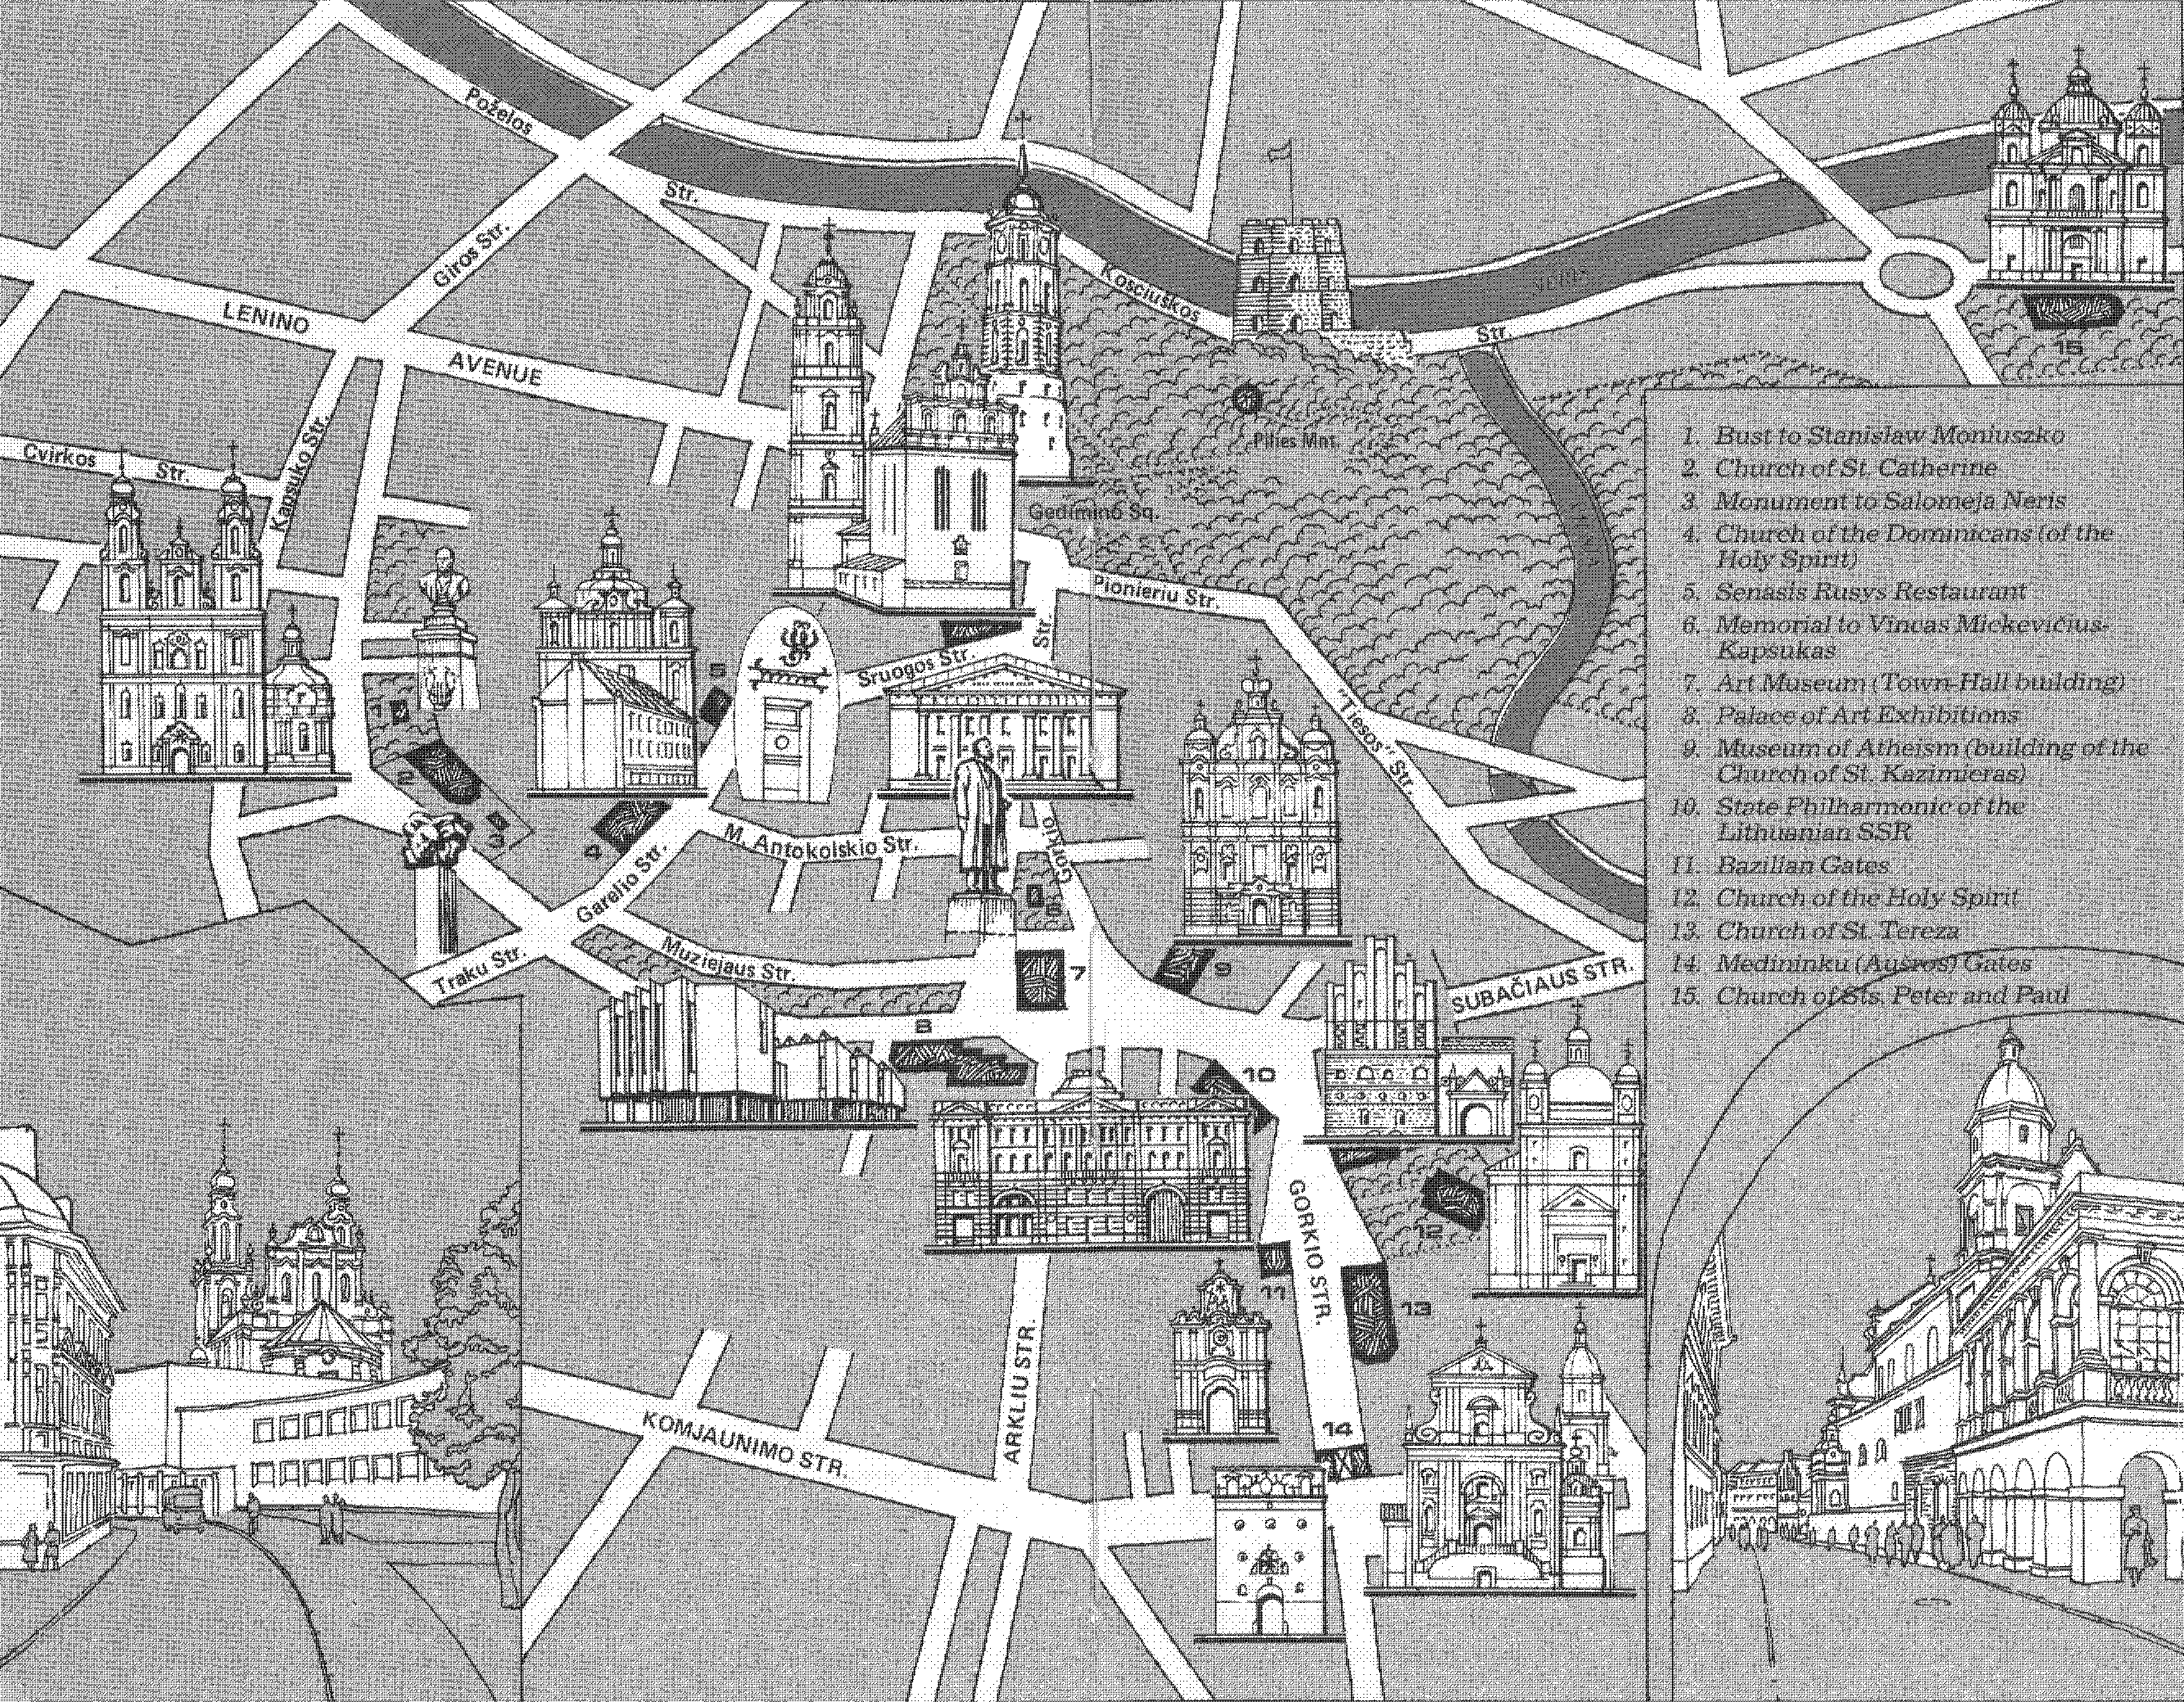
\includegraphics[width=\textwidth]{ilustra-10.png}
%    \captionsetup{format=plain,labelsep=newline,justification=centering}
    \caption{Mapa com plano turístico da Vilna soviética, de 1981. Apesar da ideologia marxista-leninista do regime soviético, as igrejas definiam a paisagem urbana e eram a visão mais proeminente da cidade. Durante os anos do regime, a Igreja de São Casimiro (indicada no mapa como número 9), foi transformada no Museu do Ateísmo.}
\end{figure}

Engajamentos sociais e curiosidade política trouxeram Döblin de volta ao
presente. Quer explorar a mecânica da ideologia governante do dia:
``Consigo ver as forças que se alteram e afrouxam. Na Europa Oriental, a
emancipação das massas ocorre num contexto nacionalista --- na verdade, a
maior ênfase recai sobre o nacionalismo.''\footnote{Ibid., p. 103.} Nota
que ``os milhões de judeus estão desenvolvendo um novo senso de nação
europeia livre, livrando"-se do antigo peso da sujeição e do desdém. Eles
querem se tornar minoria nacional ou então tomar emprestado o velho lar
asiático da sua religião.''\footnote{Ibid., p. 109.} Dotado de tal
reflexão, o escritor mergulha no \textit{Zeitgeist} da \textit{Vilne} judaica.


O escritor visita a organização sionista e o Bund, vai a escolas de
hebraico e iídiche e, em seguida, identifica o dilema judaico essencial
da era moderna: ``não é só Baal"-Shem \textit{versus} o estado, mas também
Oriente \textit{versus} Ocidente. A primeira fratura da nação judaica:
Gaon, Baal"-Shem \textit{versus} política secular. A segunda fratura entre
os judeus emancipados: apoiadores do estado burguês \textit{versus}
socialistas. Os socialistas --- universais, humanistas, internacionais ---
mantêm melhor a velha corrente do Gaon, a grandiosa ideia
supranacional.'' Ele também descobre similaridades ideológicas entre os
promotores do iídiche e os defensores do hebraico: ``Ambos são modernos,
nacionalistas, ocidentais.'' Nutre grande desconfiança pelos grupos
sionistas, mas sente"-se imediatamente à vontade com o Bund, proponentes
da língua iídiche.\footnote{Ibid.}

\asterisc

Döblin ficou evidentemente impressionado com a diversidade cultural e
vitalidade política do universo judaico da cidade. Viu no Gaon de \textit{Vilne}
um modelo da judiaria moderna --- racional e diligente, mas com um
compromisso inabalável para com a vida espiritual. Temia porém que a
ideia de um estado judaico pudesse funcionar contra os princípios dos
ensinamentos do Gaon. O nacionalismo, em sua opinião, poderia obliterar
a espiritualidade dos judeus:

\begin{quote}
Não posso deixar de pensar ao sair: Que nação impressionante são os
judeus. Não conhecia essa nação: achava que aquilo que eu tinha visto na
Alemanha, achava que os judeus fossem pessoas trabalhadoras, lojistas,
que labutam em prol da família e aos poucos ficam gordos demais,
intelectuais ágeis, incontáveis pessoas sofisticadas, infelizes e
inseguras. Agora percebo que se trata de exemplos isolados, degenerados,
distantes do núcleo da nação que aqui vive e se mantém. E que núcleo
extraordinário é este, que produz indivíduos como o rico e transbordante
Baal"-Shem, a chama mística do Gaon de \textit{Wilno}. Que acontecimentos
ocorreram nestas áreas orientais aparentemente incultas. Como tudo flui
em torno do espiritual!

[\ldots{}] E se o fluxo da história se invertesse e Sion fosse realmente
concedida aos judeus? E isso está se tornando uma questão urgente. As
velhas condições artificiais não se podem mais manter, seu rigor é
debilitante. A era moderna e as necessidades econômicas estão conduzindo
os judeus para fora de sua reclusão. O movimento inverso está em curso.
A tragédia do cumprimento está em curso. O templo que encontrarão caso
busquem não será mais o Templo. Os religiosos, os espiritualizados sabem
disso. Eles dizem: Só o Messias pode nos conceder o Templo. Os judeus
mais genuínos deixaram de esperar pelo `estado' faz tempo. Só é possível
se preservar no campo espiritual; é por isso que é necessário permanecer
no espiritual. A política não tem como trazer o mundo celestial, a
política não produz nada além de política. A era `moderna' não apresenta
quaisquer problemas aos judeus.

Contudo, as circunstâncias externas atuais, políticas e econômicas, e a
situação difícil das massas, são fatos. O velho organismo mobilizará uma
forte resistência a toda mudança. `Estado' e `Parlamento' assomam no
horizonte --- contra o Gaon e o Baal"-Shem.\footnote{Ibid., pp. 102--103.}
\end{quote}

Durante o quarto e último dia da visita, Döblin foi levado ao velho
cemitério judaico, localizado bem do outro lado do rio, em frente à
Colina do Castelo. ``O cemitério judaico,'' escreve Israel Cohen em sua
história de \textit{Vilne}, de 1943, ``no linguajar tradicional dos judeus
ortodoxos, é \textit{Bet `Olam}, `Casa da Eternidade,' termo que
combinaria o amor pelo eufemismo com a fé na imortalidade. Vilna tem
duas dessas `casas,' situadas numa distância considerável uma da outra.
O velho cemitério, do outro lado do Rio Vilia\ldots{} se estende por uma
grande área, parecendo"-se em sua maior parte com um campo abandonado,
tomado por ervas daninhas; pois o número de lápides é comparativamente
pequeno.''\footnote{Cohen, op. cit., p. 415.} Esses cemitérios tinham
uma função importante --- narravam e guardavam o passado judaico local.
``A maioria dos judeus de Vilna,'' relembra Lucy Dawidowicz, residente
judia americana da cidade, ``sabia de sua própria história nem tanto a
partir da leitura de livros, mas da visita aos dois cemitérios judaicos,
onde a história estava literalmente sepultada. [\ldots{}] Segundo a
tradição, os judeus usavam {[}o velho cemitério{]} como terreno de
sepultamento desde 1487, mas os primeiros registros históricos datam de
1592. Em 1830, as autoridades russas fecharam o cemitério por falta de
espaço.''\footnote{Lucy Dawidowicz, \textit{From That Place and Time: A Memoir, 1939--1947}. Nova York: W.\,W. Norton \& Company, 1989, pp. 48--49.}

As necrópoles seduzem Döblin: ele foi ao cemitério judaico de Varsóvia
no Dia do Perdão. Estava tomado por uma massa irrequieta de mulheres
lamentando e homens rezando. Döblin ficou horrorizado: ``Calafrios sobem
e descem pela minha espinha ao ver e ouvir essas coisas. [\ldots{}]
Trata"-se de algo primordial, atávico. Terá isso algo a ver com o
judaísmo? [\ldots{}] São resquícios de uma religião diferente, animista,
um culto aos mortos.''\footnote{Döblin, \textit{Journey to Poland}, op. cit., p. 66.} A visita ao velho cemitério de \textit{Wilno} lhe fornece um testemunho contrastante da vida judaica.

Döblin vai à velha necrópole com dois jovens guias, ativistas do
movimento juvenil iídiche. O portão do cemitério está trancado e, como
três adolescentes levados, eles o arrombam. O escritor de meia"-idade se
diverte copiosamente: ``é algo terrível a dizer --- rimos, rimos sem parar
ao entrar no cemitério, deixando às pressas o portão atrás de
nós.''\footnote{Ibid., p. 111.} O lugar abandonado o hipnotiza com sua
devoção ordinária, sua proximidade mundana de Deus e sua melancólica
solidão. Pela primeira vez --- de fato, a única ao longo do relato
impressionista da Polônia --- Döblin deixa inacabados seus pensamentos.
Abandona o fluxo narrativo diante do túmulo do Gaon, como se esperasse
por um pensamento estimulante depois do ciclo interminável de
reassentamentos e exílios caóticos:

%{[}figura 69{]}
%
%O velho cemitério judaico em Vilne.
\begin{quote}
Aqui, encontramos um imenso gramado com várias árvores e, irregulares,
aqui e ali, solitárias ou em grupos, lousas baixas de pedra. Folhas
secas por toda parte, até mesmo amontoadas em algumas reentrâncias. Uma
garoa fina cai. As tábuas de pedra ostentam inscrições compridas,
escritos angulosos em hebraico, em vermelho e amarelo. Leões são
retratados com frequência nas lousas. Estilhaços, fragmentos de pedra
jazem em derredor. Terrível o descuido do cemitério. Pedaços de tijolo,
pedrinhas sobre diversos túmulos. Palha por debaixo das pedrinhas, e
também bilhetes escritos em hebraico. Representam a passagem de judeus
devotos que por ali rezaram. Pois eles viajam de longe para rezar junto
aos túmulos de homens célebres, homens sagrados. Um sentimento profundo
e obscuro os conduz até ali. De alguma maneira --- eles acham, eles sentem
--- o homem sagrado ainda está junto a seu túmulo, a seu corpo, e eles
podem se aproximar dele assim como seus ancestrais faziam no tempo em
que ainda vivia. O morto está amarrado a seu túmulo, sua alma
desaparecida, amarrada a seu cadáver, e sua alma pode ser evocada por
intermédio da oração. E o devoto, o rebe, os santos estão mais próximos
de Deus e conseguem obter mais dEle do que um homem comum, talvez como
se agissem como Deus. Como está tudo dilapidado por aqui. Ouço gritos,
ordens, soldados cantando e, de repente, um mugido. Subo numa pequena
elevação, sobre a qual placas de pedra se espalham, aos pedaços. Lá de
cima, avisto uma vaca pastando mais abaixo. Pastando por cima dos
túmulos. Seu rastro está por toda parte.

[\ldots{}] Os judeus de \textit{Wilno}, a meu ver, são orgulhosos, mas só em parte
e de uma maneira muito oriental. A grama cresce alta e selvagem. Nos
montículos, tropeça"-se sempre em lápides despedaçadas. Elas em geral
exibem belos leões de caudas rodopiantes, antigo símbolo de força. A
tumba do Gaon de \textit{Wilno}. Uma casa baixa de pedra, rodeada por uma cerca
de barras de ferro, está trancada. Contém seu túmulo e os túmulos de
seus parentes e amigos próximos. Jaz ali junto com toda essa gente, que
em vida ele nem conheceu tão bem. Quando a esposa morreu, ele disse ``Eu
tinha que passar fome com frequência, mas o fiz pela Torá e por Deus.
Mas você passou fome por mim, um ser humano.'' Pilhas inteiras de
bilhetinhos cobrem sua lápide e o chão em derredor. Estão dependurados
também do lado de fora, na grade de ferro, amarrados às barras com fios
de palha e relva\ldots{}\footnote{Ibid., pp. 111--113.}
\end{quote}

A \textit{Wilno} de Döblin é uma colagem de impressões irregulares, pensamentos
justapostos e contradições descritivas. Mas esse estilo literário
reflete o espírito narrativo moderno e expressionista. Deve"-se ler o
retrato que faz da cidade não como imagem inequívoca, mas como marca
cartográfica. Um mapa jamais é uma representação completa ou confiável
de um lugar: ele é a projeção de uma imaginação factual, que só faz
sentido se lermos, compreendermos e seguirmos a respectiva legenda
cartográfica.

A admiração do escritor pelos judeus de \textit{Vilne} perdurou por toda a vida.
Depois do Holocausto, ele situou o encontro com aquele mundo
desaparecido entre suas mais queridas experiências: ``Estive na Polônia.
Escrevi um livro sobre isso. Fui lá e, pela primeira vez na vida, vi
judeus. Fiquei profundamente comovido à visão deles. Jamais esqueci o
que vi nos guetos de Varsóvia, de \textit{Wilna} e Cracóvia\ldots{}'' Contudo,
Döblin considerou ter fracassado na tentativa de desfazer a lacuna entre
ele e os ideais deles. No fim, a seu ver, o custo de ter sobrevivido ao
grande reassentamento foi outra forma de alienação. Ele resumiu seu
breve flerte com a modernidade iídiche de \textit{Wilno} com uma afirmação
derrotista: ``Minhas palavras nada significaram. Nada senti. Foi mais
uma bandeira que não pude empunhar.''\footnote{Döblin, \textit{Destiny's Journey}, op. cit., pp. 110--111.}

%{[}figura 70{]}
%Distâncias a partir de Vilna
%Países vizinhos
%Kaliningrado 318km
%Minsk 215km
%Riga 300km
%Varsóvia 450km
%Outras grandes cidades
%Berlim 1035km
%Londres 1751km
%Moscou 875km
%Nova York 6929km
%Paris 1690km
%Vilna no centro da Europa.

\chapter[Redemoinho europeu \medskip]{Redemoinho europeu}

%\setlength{\epigraphwidth}{.45\textwidth}
\begin{epigraphs} 
\qitem{E mais uma vez percebo que é mais fácil um ser humano mudar do que uma
cidade. O ser humano é capaz de se transformar. A cidade desmorona.}{\textsc{alfred döblin}}
\end{epigraphs}

Enquanto escrevia este livro, a localização exata do centro geográfico
da Europa se moveu mais uma vez. De acordo com as novas conclusões
científicas obtidas (de novo) pelo Instituto Geográfico Nacional
Francês, o centro continental se situa agora a 54 graus e 50 minutos de
latitude, e 25 graus e 18 minutos de longitude. Esse novo cálculo se
baseia na exclusão de algumas protuberâncias políticas da Europa, tais
como as ilhas dos Açores, as ilhas Canárias e Madeira que, em termos de
base geotectônica, pertencem à África, e algumas das ilhas gregas do
lado asiático do Mar Egeu. Esses pequenos ajustes cartográficos
estreitaram os tênues limites da Europa e também situaram o epicentro
continental para mais perto de \textit{Vilnius}, a apenas seis quilômetros ao
norte da Cidade Velha. Apesar do deslocamento, o significado
comemorativo do antigo centro permanece o mesmo. O monumento erguido
para marcar a entrada da Lituânia na União Europeia ainda adorna o
centro anterior, mesmo se sua mensagem simbólica tenha se engendrado
baseando"-se num erro de cálculo científico de breve duração.

A \textit{Vilnius} do século \textsc{xx} muito se assemelha ao centro geográfico da
Europa: sempre inconstante, recalculada, remapeada e todavia jamais
capaz de alcançar um significado fixo ou localização estável. A era
moderna trouxe a \textit{Vilnius} não só guerras, ocupações estrangeiras,
revoluções, ideologias conflitantes, massacres, despovoamento,
depressões econômicas e ciclos irregulares de modernização; ela criou
também as condições propícias para conversões e más interpretações da
memória. A \textit{Vilnius} moderna se ergue sobre uma pretensão histórica, uma
ideia deliberadamente construída de que o passado não tem testemunhas
permanentes, apenas ruínas que podem se desmanchar, ser refeitas e de
novo dispersas. A \textit{Vilnius} contemporânea é uma cidade sem descanso --- não
em termos de seu presente, ou mesmo de seu futuro, mas de seu próprio
passado. É um lugar repleto de ruínas, como uma velha necrópole em que
os mortos antigos competem por espaço e memória com os que chegaram há
menos tempo. Por puro acaso, o novo centro da Europa caiu num alqueive
recentemente revitalizado para servir às crescentes necessidades locais
do mercado de pompas fúnebres. Um casarão abandonado, transformado num
dinâmico ateliê de produção de lápides tumulares, obscurece o coração da
Europa.

Os habitantes de \textit{Vilnius} respeitam os \textit{próprios} mortos. É um
costume profundamente arraigado, que se origina de uma variedade de
tradições religiosas e culturais. Uma morte que não produz um túmulo bem
demarcado é considerada um destino deplorável e mesmo cruel. As práticas
modernas da cremação, funerais sem sepultura, aluguel de jazigo,
transposição de restos mortais e necrópoles despersonalizadas, tradições
populares em quase toda a Europa e América do Norte, são simplesmente
vistas como bárbaras pelos locais. Os cemitérios de \textit{Vilnius} ainda são
planejados e conservados como locais eternos, alocados perpetuamente aos
mortos e seus parentes vivos. Como resultado, os cemitérios, sempre em
expansão, invadem boa parte dos espaços verdes da cidade, fazendo dela
um dos lugares mais necrológicos da Europa.

Durante o século \textsc{xx}, a necrópole de \textit{Vilnius} ganhou grande proeminência
junto aos moradores da cidade e também seus visitantes. As ruínas podem
não falar, elas no entanto moem pergaminhos incompletos e inacabados de
história de maneira profunda no terreno dos acontecimentos. Na ausência
de uma narrativa histórica coerente e uma localização geográfica
estável, os mortos se transformam nos indicadores mais evidentes da
identidade da cidade. Em 1938, um visitante americano foi guiado por um
dos mais antigos cemitérios católicos da cidade na primeira manhã de sua
visita:

\begin{quote}
Sem termos tomado o café da manhã, fomos catapultados para ver a tumba
conjunta de Pilsudski e sua mãe e em seguida a missa matutina na Ostra
Brama, um dos mais célebres templos da Polônia. Ficava apenas a cinco
minutos de carro da estação até o assim chamado cemitério Rossa, em cujo
canto fica a tumba, à qual se tem acesso por uma generosa escadaria. Uma
laje de mármore negro polido instalada na plataforma de concreto marca o
memorial de mãe e filho, impressionante em sua extrema simplicidade. Uma
falange de cruzes brancas --- duzentas delas --- margeiam o túmulo de ambos
os lados, epitáfios silenciosos dos heróis que tombaram por \textit{Wilno}
defendendo o país. Cada um em pé de cada lado do memorial, dois soldados
do exército polonês vigiam perpetuamente os mortos. Tão imóveis eram
eles em seu uniforme cáqui e tanto se pareciam com estátuas de bronze
que só depois de algum tempo percebemos que eram soldados vivos da
República. [\ldots{}] Passeamos pelo cemitério analisando os túmulos,
antigos e recentes, dos falecidos habitantes de \textit{Wilno}. Apesar das áreas
lotadas de seus acres, o cemitério possui vários elementos de beleza
natural; ele ocupa a encosta de uma colina e suas características
naturais foram todas conservadas. Colinas e vales em miniatura
recobertos por árvores e arbustos, falésias e penhascos diminutos
brilhando de flores silvestres e plantas alpinas dão sua contribuição
para o charme desse campo"-santo singular. Não somos especialistas em
cemitérios e talvez o costume ali seguido não seja exclusivamente
polonês, mas de certo modo nos surpreendeu o realismo empregado pelos
parentes dos mortos: uma fotografia do falecido, emoldurada e protegida
das intempéries, está afixada em muitas das pedras tumulares.\footnote{Robert Medill McBride, op. cit., pp. 113--117.} 
\end{quote}

Na cripta da catedral, mostraram aos turistas americanos o
recém"-descoberto corpo de Sigismund Augustus, rei da Polônia e
grão"-duque da Lituânia do século \textsc{xvi}, e de sua amada esposa, Barbara
Radziwiłłowa (Radvilaite). Em seguida, foram levados a um espetáculo
ainda mais mórbido, escondido nas passagens subterrâneas da cidade
velha:

\begin{quote}
Ouvíramos falar de uma notável coleção de múmias na cripta da Igreja do
Espírito Santo, parte de um mosteiro dominicano fundado em 1597. Mas
estávamos mal preparados para a visão macabra por ocasião da nossa
chegada à igreja. Na cripta sombria, acessada por uma escadaria de pedra
no pátio do velho mosteiro, ficamos frente a frente com uma multidão de
corpos mumificados e esqueletos de santos e pecadores que haviam deixado
esta vida centenas de anos atrás. Os corpos haviam antes repousado
ordenadamente em seus ataúdes na catacumba da igreja. Mas agora se
alinhavam numa complexa desordem na escuridão das abóbadas subterrâneas.
Tal falta de respeito à santidade dos mortos é uma acusação feita às
desumanidade dos russos; pois muito antes da Grande Guerra, numa das
esporádicas eclosões de atividade revolucionária polonesa, prisioneiros
políticos eram presos em tal número que sobrecarregaram a ocupação
máxima dos presídios da cidade. A cripta dominicana, grande, espaçosa,
profunda e adequadamente escura, encantou os senhores moscovitas mais
como alojamento para os vivos do que lugar de descanso para os mortos.
Os ataúdes foram removidos e enfileirados no chão de terra do rudimentar
porão abobadado. Contudo, a madeira dos ataúdes já estava debilitada
pelos anos e incapaz de suportar o processo de remoção. Como resultado,
muitos deles se abriram e expuseram seus ocupantes, que se encontravam
em surpreendente estado de preservação. É claro que se produziu espaço
no porão e, quando foi necessário acomodar mais gente, a cripta
continuou expelindo seus silenciosos habitantes. As autoridades russas
estavam obviamente demasiado indiferentes ao bem"-estar dos defuntos para
construir prateleiras nas paredes a fim de arranjar o fluxo de ataúdes.
Após escolherem um nicho profundo sob os arcos, eles removeram os corpos
dos caixões e, sem qualquer cerimônia, empilharam"-nos naquela fenda
escura. Lá estão eles agora, literalmente às centenas, em sua maior
parte simples esqueletos, jazendo caóticos num gigantesco amontoado; os
da parte superior assumiram posições fantásticas, com as cabeças,
braços, pernas, mãos e pés se projetando em todos os ângulos num arranjo
macabro.

Os corpos que obtiveram a gentil permissão de permanecer em seus caixões
se encontram bem mumificados e vários podem ter a idade, sexo e posição
identificados. Observamos uma mulher pertencente à nobreza, reconhecível
pelos fragmentos de roupa e joias; outro de uma senhora idosa; um
cavalheiro enfeitado com tufos de cabelo e resquícios de um bigode, mas
desvestido; e ainda outra mulher, dona de um anel de ouro que havia sido
roubado da mão sem vida e mais tarde devolvido pelo gatuno de
consciência pesada. Sobre algumas mesas estavam roupas centenárias de
padres e freiras, pois este edifício gozou de uma longa história de
centro eclesiástico; botas dos pés dos soldados de Napoleão, que
morreram na retirada de Moscou; e objetos vários encontrados no entulho
da cripta.\footnote{Ibid., pp. 130--132.}
\end{quote}

%{[}figura 71{]}
%
%Rua Zamkowa (do Castelo) em \textit{Wilno}, ca. 1930.

Em meados do século \textsc{xx}, \textit{Wilno} chegou a ser vista como materialização de
uma Europa anacrônica em que um passado remoto e esquecido havia
persistido até a era moderna. A primeira impressão de Lucy Dawidowicz
sobre a cidade foi a de um lugar romântico, matizado por um exotismo
histórico. ``Ainda mais atraentes para o turista americano afeito à
história foram as ruínas medievais de Vilna, visíveis por toda parte nas
ruas e colinas. Foi uma cidade cuja história se perde na noite dos
tempos. Para mim, Vilna era a quintessência do Velho Mundo, um lugar
lendário com um passado lendário.''\footnote{Lucy Dawidowicz, op. cit., pp. 28--29.} O caráter de palimpsesto não era ao gosto de todos. Em julho de 1940, Ann Louise Strong, jovem ativista do sindicato
trabalhista britânico, passou brevemente pela cidade em viagem rumo a
Moscou. Ela resumiu o enquadramento peculiar de sua localização
geográfica; ``Quem quer que solucione o problema de Vilna é capaz de
solucionar o problema da Europa. Vilna é um misto insolúvel de ódios
nacionais {[}e{]} um exemplo mundial --- há vários deles na Europa --- da
insolubilidade do problema dos ódios nacionais sob o domínio
capitalista.''\footnote{Anne Louise Strong, \textit{Lithuania's New Way}. Londres: Lawrence \& Wishart, 1940, p. 31.} Ao mesmo tempo, ela foi cinicamente informada por um diplomata americano de que a ``única coisa
a se fazer com Vilna é pegá"-la, levá"-la para longe, espremer as pessoas
cada uma para sua respectiva nação e depois colocar a cidade num
museu.''\footnote{Ibid.}

A troca de rótulos chegou primeiro. A cidade mergulhou na Segunda Grande
Guerra em 1 de setembro de 1939, como \textit{Wilno}, cidade polonesa; emergiu
dela em 1945 como \textit{Vilnius}, capital da República Soviética da Lituânia.
Seguiram"-se mudanças de nomes de lugares, posto que a predominância
cultural e demográfica das línguas polonesa e iídiche foi substituída
pela supremacia ideológica e administrativa das línguas russa e lituana.
A transformação foi pontuada por ocupações de diferentes colorações
nacionais e ideológicas. De acordo com os protocolos secretos do Pacto
Nazi"-Soviético de 1939, a cidade, junto com a parte oriental da Polônia,
foi ocupada pela União Soviética, que, por razões estratégicas,
devolveu"-a à Lituânia. Por meio ano, \textit{Vilnius}, repentinamente capital
legal porém ainda não administrativa da neutra Lituânia, permaneceu num
limbo geopolítico surrealista. Isolada do resto da Europa pela guerra
abrangente, a cidade se tornou abrigo precário de milhares de refugiados
judeus e poloneses que corriam das ocupações nazista e soviética da
Polônia. Herman Kruk, médico judeu de Varsóvia, estava entre aqueles que
conseguiram escapar dos bombardeios nazistas e que chegaram à cidade
cruzando a zona controlada pelos soviéticos:

\begin{quote}
As centenas e milhares de pessoas que chegaram a Vilna estavam
amontoadas, apavoradas, famintas e exaustas. Curvadas --- devido ao hábito
de se inclinar ao som de cada bomba explodindo. Apavoradas devido a tudo
aquilo que ocorre ao redor delas com tanta rapidez, tanto terror e
tragédia. [\ldots{}] O mar transbordou e inundou Vilna. Um lugar para se
deitar é um sonho. Um naco de pão é uma raridade. Uma camisa --- quem
pensa em camisas? [\ldots{}] Sabão é um luxo. Comida quente, uma quimera.
Qualquer quarto que se pareça normal nos faz estremecer: um quarto!? As
pessoas ainda têm quartos? [\ldots{}] Ainda há pessoas dormindo em camas?
[\ldots{}] Ainda há pessoas dormindo? Todo refugiado estremecia ao ver que
a vida normal em algum lugar ainda segue seu ritmo e que nem tudo está
destruído e esmagado. [\ldots{}] Eles então se arrastavam pelas ruas de
Vilna, refugiados vindos de toda a Polônia. Trabalhadores de Varsóvia,
alunos de \textit{yeshivá} de Lublin, comerciantes de Katowice, engenheiros,
médicos --- rastejando pelas vielas medievais de Vilna, à procura de
abrigo. Em busca de uma porta aberta, de um pouco de água para se lavar,
uma tábua onde se deitar. Por cima de tudo isso, as sirenes de alarme.
Cada um reagia a seu modo e cada um queria ajudar de alguma maneira,
mas\ldots{} Vilna estava ocupada com seus próprios problemas, sua
própria angústia e sofrimento. Vilna tinha acabado de se livrar do
pesadelo da guerra, do bombardeamento alemão, das noites escuras e dias
mortais. Amputada do resto do mundo, Vilna estava com fome e ninguém
naquela época se importava com os refugiados.\footnote{Herman Kruk, \textit{The Last Days of the Jerusalem of Lithuania: Chronicles from the Vilna Ghetto and the Camps 1939--1944}, trad. Barbara Harshav. New Haven: Yale University Press, 2002, pp. 28--29.}
\end{quote}

O controle lituano sobre \textit{Vilnius} durou pouco. Em 15 de junho de 1940, um
dia depois da entrada do exército alemão em Paris, a Lituânia foi
ocupada pelas tropas soviéticas. Em dois meses, a Lituânia Soviética
junto com sua capital, \textit{Vilnius}, se tornou estado membro da \versal{urss}, mas o
exército alemão tomou a cidade numa \textit{Blitzkrieg} em 24 de junho de
1941, três dias após o início da invasão nazista da União Soviética.
Yitskhok Rudashevski, menino judeu de 14 anos com ligações com o partido
comunista, observou que ``à noite, um lituano armado anda pelas ruas
tristes e vazias da cidade velha. [\ldots{}] Ao alvorecer, passa uma
motocicleta. Um capacete cinza de aba quadrada, óculos, sobretudo e
rifle. Infelizmente, o primeiro soldado do exército usurpador alemão que
fui capaz de ver. O capacete cintila gélido e maligno. Um pouco mais
tarde desço até a rua {[}onde{]} me encontro com um camarada. E
caminhamos como estranhos pelas ruas largas. O exército alemão está
marchando. Permanecemos ambos em pé, de cabeça curvada. Uma miragem
soturna de tanques, motocicletas, armamento.'' Em 8 de julho, ``foi
publicado o decreto pelo qual a população judaica de Vilna deve usar
distintivos na frente e atrás --- um círculo amarelo com a letra J dentro.
O dia está nascendo. Olho pela janela e vejo diante de mim os primeiros
judeus de Vilna com distintivos. Foi doloroso ver como as pessoas os
fitavam. [\ldots{}] Fiquei com vergonha de estar entre eles na rua, não
porque se notaria que sou judeu, mas por eu ter vergonha daquilo que
{[}eles estavam{]} fazendo conosco.'' Dois meses depois, ``um nascer do
dia belo e ensolarado. As ruas foram fechadas pelos lituanos. Há
turbulência nas ruas. Trabalhadores judeus têm permissão de entrar. Está
sendo criado um gueto para os judeus de Vilna.'' No tumulto, Rudashevski
foi empurrado para dentro do portão do gueto: ``Sinto como se tivesse
sido roubado, como se roubassem minha liberdade, minha casa e as ruas
familiares de Vilna que tanto amei. [\ldots{}] Ouço a respiração ofegante
de gente com quem fui subitamente amontoado, gente que, como eu, foi
subitamente arrancada de casa.'' No primeiro dia no gueto, oficiais
alemães vieram fotografar ``as ruas tortuosas, as pessoas assustadas.
Deliciam"-se na Idade Média que eles mesmos transportaram para o século
\textsc{xx}!!!!''\footnote{Yitskhok Rudashevski em Laurel Holliday ed., \textit{Children in the Holocaust and World War \versal{ii}: Their Secret Diaries}. Nova York: Pocket Books, 1995, pp. 140--147.}

O gueto, escreve Kruk, estabelecido na parte antiga da cidade, ``zumbe
como uma colmeia. Uma área planejada para 3 ou 4 mil pessoas é agora
ocupada por dezenas de milhares. Cabeças sobre cabeças. Um em cima do
outro. Menos de um metro por pessoa, pior do que num cemitério.'' A
densidade claustrofóbica dos edifícios superlotados eclode para fora.
``Cada pátio é uma rua. Cada rua é uma cidade. Um formigueiro
fervilhante: empurrões, perseguições, atropelos --- dor extrema.'' Apesar
da fome, das enfermidades e das recorrentes \textit{Aktions} de matança
alemãs, a população do gueto jamais diminui. Os mortos e assassinados
são substituídos por recém"-chegados de outras comunidades judaicas.
Enquanto em 1943 apenas um punhado de judeus locais permanecia no gueto,
``havia uma mescla de gente expulsa das cidades vizinhas, ou fugitivos
de massacres, de praças de execução, de remoções, de buracos e
esconderijos. Haviam passado por horror e aflição, haviam sido
purificados pela dor, haviam retornado do inferno. São selvagens e
atrevidos. Embora a morte nada seja para eles, o suicídio não está nos
seus cálculos.'' Para eles, \textit{Vilne} ``é o refúgio derradeiro. Um lugar de
desafios, de não deixar passar.''\footnote{Kruk, op. cit., pp. 656--657.}
Apesar do horror diário, uma sensação surrealista de normalidade torna a
vida mais fácil. ``Às vezes fico ocupado por horas,'' anota Rudashevski
em seu diário. ``É difícil concluir algo na escola e no clube, e ao
mesmo tempo ainda se dedicar à cozinha e à faxina. Na escola estamos
agora estudando Vilna em geografia.''\footnote{Rudashevski, op. cit., p. 181.}

A vasta maioria dos judeus de \textit{Vilne} foi assassinada pelos alemães e
colaboradores lituanos em Ponary (Paneriai), a colina verdejante do
outro lado da cidade, onde o exército napoleônico encontrou o próprio
fim em 1812. O gueto foi liquidado em 23 de setembro de 1943, e a maior
parte dos onze mil habitantes que ainda restavam foi enviada para campos
de concentração na Estônia, onde poucos sobreviveram ao trabalho forçado
e à fome. Dos sessenta mil judeus locais, não mais que três mil viram o
fim da guerra. No verão de 1944, logo após os ocupantes nazistas terem
sido rechaçados pelo exército soviético, quando o escritor iídiche Chaim
Grade (1910--1982) voltou do exílio forçado na Ásia Central para o bairro
de infância em \textit{Vilne}, ele instantaneamente se sentiu estrangeiro. \textit{Vilne}
não existia mais: a cidade judaica não era nem mesmo um museu ou um
cemitério, mas um fantasma, uma memória inquieta desprovida de um abrigo
que pudesse chamar de lar, um espírito sem corpo. ``Desde o meu retorno
a Vilna,'' escreve Grade, ``perambulei pelas sete vielas que no passado
formaram o Gueto. As ruelas estreitas me enredavam e aprisionavam, como
passagens subterrâneas, como cavernas repletas de túmulos antigos.
Órfãs, elas lançaram um feitiço sobre mim; seu vazio ronda meu cérebro,
elas aderiram a mim como sete correntes de pedra. Não tenho, contudo,
nenhum desejo de me livrar delas. Quero que se embrenhem cada vez mais
fundo no meu corpo, na minha carne. Sinto a rigidez gélida e sombria de
portões aferrolhados e de portas que rangem sob minha pele. Meus olhos
são vidraças estilhaçadas, e alguém dentro de mim grita em voz alta:
`Que seja! Quero me tornar uma ruína!'"\footnote{Chaim Grade, \textit{My Mother's Sabbath Days}, trad. Channa Kleinerman Goldstein e Inna Hecker Grade. Nova York: Alfred A. Knopf, 1986, p. 335.}

Enquanto \textit{Vilne} soterrava na carne dos sobreviventes que levavam suas
memórias para todos os cantos do mundo, \textit{Vilnius} foi rapidamente populada
por novos residentes. Alguns vieram de outras cidades lituanas e do
interior desmoralizado e assolado pela violência (a resistência lituana
contra a ocupação soviética continuou por anos após o fim da Segunda
Grande Guerra, e deportações maciças da população local cessaram apenas
com a morte de Stálin em 1953). Outros chegaram de mais longe, sobretudo
da Rússia. A sovietização e a \textit{lituanização} dos topônimos locais ajudaram
na aclimatação dos recém"-chegados. Mas enquanto a antiga predominância
das línguas polonesa e iídiche foi substituída pela autoridade
administrativa do russo e lituano, os novos habitantes da cidade jamais
se sentiram à vontade em casa. O poeta lituano Tomas Venclova lembra"-se
de chegar quando criança a \textit{Vilnius}, depois da guerra. ``Era uma cidade
completamente estranha'' para quase todos os lituanos, e a ``vida em
Vilnius no início foi um árduo enraizamento num solo novo. Em geral, foi
caótico.''\footnote{Tomas Venclova em Czesław Miłosz, \textit{Beginning with My Streets}, trad. Madeline \textsc{g}.\,Levine. Nova York: Farrar Straus Giroux, 1991, p. 40.}

%{[}figura 72{]}
%
%Ruínas de \textit{Vilnius} do pós"-guerra, com as igrejas barrocas ilesas, ca.
%1947.

A metamorfose histórica encobre o colapso humano da cidade: na década
durante e após a guerra (1939--1949), por meio de assassinato,
deportação, exílio, repatriação e emigração, \textit{Vilnius} perdeu quase
noventa por cento da população. Com a comunidade judaica aniquilada e
muitos dos habitantes poloneses forçados a abandonar a cidade para a
recém"-reconfigurada Polônia, a \textit{Vilnius} lituano"-soviética se transformou
num lugar inócuo, não muito diferente de um museu, mas sem reconhecer
seu passado recente. Com o tempo, e livre do terror stalinista, uma nova
cidade surgiu. Ainda multinacional, apesar da dramática mudança na
composição étnica, \textit{Vilnius} cresceu como o coração em coma da nação
lituana reprimida e, logo antes do colapso da União Soviética, a
população falante de lituano, pela primeira vez na história moderna,
atingiu maioria demográfica.

Um dos trágicos paradoxos do período da Segunda Grande Guerra foi o fato
de que \textit{Vilnius} não só perdeu a maior parte de seus habitantes, como
também perdeu quase todas as suas memórias e narrativas. Décadas a fio
houve mais nativos da cidade, ou seja, pessoas que nasceram e viveram em
Vilnius antes da guerra, que viviam fora dela do que nela própria. A
Vilnius soviética foi em grande parte uma cidade de imigrantes, cujos
laços familiares com a cidade eram débeis e cujo conhecimento pessoal do
lugar era superficial. Sem dúvida, muitos dos novos residentes,
sobretudo lituanos e russos mas também alguns poloneses e judeus, amaram
a cidade e se sentiram orgulhosos de seu passado, mas, sob o restritivo
regime soviético, sua memória da cidade jamais pôde cruzar totalmente as
fronteiras políticas do mundo dividido. O deslocamento resultou numa
mudança de identidades locais: uma geração de residentes imigrantes de
Vilnius sabia muito pouco de seu passado recente, ao passo que os velhos
habitantes e descendentes, removidos do lugar, não raro se sentiam ainda
parte da cidade. De certo modo, a linha que separa nativos e
estrangeiros foi invertida: um nativo virou um estrangeiro --- um
recém"-chegado se tornou um habitante local. Essa inversão demográfica
alterou a personalidade da cidade, fazendo da \textit{Vilnius} contemporânea, nas
palavras de um poeta lituano, um lugar andrógino, em transformação
constante, mas estéril ao mesmo tempo:

\begin{verse}
A cidade\\
muda de sexo\\
após a ruptura\\
e toda vez escapa\\
da arapuca\\
de calma contínua\\
\smallskip
{[}\ldots{}{]}\\
\smallskip
quantos poetas beijaram\\
o cabresto barroco de seda\\
tendo porém aprendido\\
uma só coisa ---\\
ir embora.\footnote{Romas Daugirdas, ``The Iron Dog, to Vilnius'', trad. Antanas Danielius, em \textit{Vilnius: Lithuanian Literature, Culture, History}, verão de 1997, p. 67.} 
\end{verse}

A maioria dos antigos habitantes poloneses da cidade foram reassentados
nas ``terras recuperadas'' da Polônia ocidental e setentrional, antigas
províncias orientais da Prússia. A Universidade Stefan Batory de \textit{Wilno},
com sua faculdade polonesa, foi transplantada para a cidade de Torun,
mas a vasta maioria dos repatriados foram instalados em Wrocław e
Gdańsk, onde as tradições folclóricas de \textit{Wilno} se entrelaçaram ao tecido
cultural da nova Polônia. A nostalgia de antigos habitantes de \textit{Wilno} foi
capturada pelo escritor alemão Günter Grass no romance \textit{Maus
presságios}, descrevendo um caso de amor entre dois expatriados: um
viúvo alemão com raízes em Danzig e uma viúva polonesa vinda de uma
família de \textit{Wilno}. Eles se encontram pela primeira vez no dia 2 de
novembro, no ano do colapso do bloco soviético, enquanto cada um
visitava túmulos de parentes no cemitério de Gdańsk. ``Eles se chamavam
de Herr Reschke e Frau Piątkowska. Descontraídos após uma troca de
olhares, de repente notaram que, por toda parte em torno deles, outras
pessoas que comemoravam o Dia de Todos os Santos prestavam homenagem a
seus mortos com flores e lamparinas. E só então a viúva fez a observação
que o viúvo viria a anotar \textit{verbatim} em seu diário: `Naturalmente,
mamãe e papai prefeririam jazer no cemitério de \textit{Wilno} a estar aqui, onde
tudo é e foi estranho.'"\footnote{Günter Grass, \textit{The Call of the Toad}, trad. Ralph Manheim. Nova York: Harcourt Brace \& Company, 1992, p. 17.} O espírito polonês (e lituano) da cidade foi também captado por inúmeras paróquias de imigrantes católicos ao redor do mundo, que
levam o nome de Ostra Brama ou Aušros Vartai, e São Casimiro.

Apesar de ter sido extremamente melancólica, a memória de \textit{Vilne} no
pós"-guerra contribuiu para o fortalecimento do espírito da resistência
nacional, continuidade cultural, tradicionalismo religioso e
transformação social dos judeus. \textit{Vilne} tem sido mantida viva nas
estórias e lembranças de famílias judaicas com raízes ancestrais na
Lituânia. Em Israel, \textit{Vilne} tem sido principalmente evocada pelos feitos
épicos dos guerrilheiros do gueto e a perseverança espiritual
transmitida pela tradição das \textit{yeshivás}. Nos Estados Unidos, \textit{Vilne} é tida
em grande conta como centro intelectual e cultural da diáspora judaica,
por intermédio de instituições acadêmicas e comunitárias tais como a
\versal{yivo}, fundada em 1925 em \textit{Vilne} mas transferida para Nova York durante os
anos da guerra, e a histórica \textit{Vilna Shul}, ``Sinagoga Vilna'', hoje restaurada em Boston. 
Na França, as tradições judaicas políticas e
intelectuais da cidade foram utilizadas por acadêmicos e ativistas
franceses da década de 1960, tais como o eminente filósofo Emmanuel
Levinas (1906--1995), que as resumiu com o lema \textit{le droit à la
différence}, ``o direito à diferença''. O termo, que desafia o ideal de
uma única cultura francesa centralizada, ecoa a sofisticação social do
ambiente iídiche da \textit{Wilno} do entreguerras, a mesma que hipnotizou
Döblin com sua habilidade de integrar a pluralidade cultural local aos
princípios universais da modernidade. Judith Friedlander, teórica
americana, capturou o espírito do clima intelectual mutante da França
num livro, \textit{Vilna on the Seine}. Na Paris pós"-1968, escreve
Friedlander, ``a Vilna judaica parece estar por toda parte: no cinema e
no teatro; nos livros e jornais; e na maneira com que os jovens
recentemente escolheram de voltar ao judaísmo, de fazer uma \textit{teshuvá}.
Inspirada pela verdade simbólica, e não histórica, Vilna (às margens do
Sena) ultrapassa os muros da Jerusalém da Lituânia. Ela reúne as antigas
comunidades judaicas que no passado viveram ao longo dos rios Neris e
Neman e do outro lado das densas florestas da Lituânia\ldots{}
abrangendo uma área conhecida como `Lite' em iídiche,'' que, depois da
guerra, foi seccionada do resto da Europa pela Cortina de
Ferro.\footnote{Judith Friedlander, \textit{Vilna on the Seine: Jewish Intellectuals in France since 1968}. New Haven: Yale University Press, 1990, pp. 5--6.}

Por trás do muro ideológico e político da separação gerada pela Guerra
Fria, os fantasmas de tempos passados foram exorcizados pelo espírito do
progresso socialista. A \textit{Vilnius} soviética, agora mimada como ``vida e
coração da Lituânia,'' foi declarada ``cidade de contrastes, mas não o
tipo de contraste que se encontra nas cidades do oeste capitalista --- não
o contraste entre o luxo da aristocracia e a pobreza dos bairros
operários; a cidade de \textit{Vilnius} é única numa rara combinação de
arquitetura moderna e monumentos de um respeitável passado.'' A paisagem
urbana de \textit{Vilnius}, conforme o alarde da propaganda soviética, ``é tão
incomum que, à primeira vista, temos a impressão de estarmos num teatro
e de que tudo aquilo é uma cenografia realizada por um artista
apaixonado pelo passado.''\footnote{G. Metelsky, \textit{Lithuania: Land of the Niemen}. Moscou: Foreign Languages Publishing House, 1959, p. 33.} Não muito diferente de sua contrapartida capitalista, a modernidade soviética se baseava no desenvolvimento de valores e padrões
universais com vistas para o futuro, mas com uma leve nuance de estética
local, nacional. Assim, a \textit{Vilnius} soviética foi planejada como ``a
capital do amanhã'', onde ``elementos da arquitetura nacional lituana se
misturam organicamente à arquitetura socialista dos novos edifícios.''
Uma cidade tão inovadora ``não tinha pares nem predecessores'' e
``qualquer um que não tenha estado em \textit{Vilnius} pelos últimos três ou
quatro anos não reconhecerá diversos cantos dessa cidade antiga e ao
mesmo tempo jovial. Em poucos anos, o panorama a partir do alto da
Colina do Castelo será novo e ainda mais belo. Mas não importa que
mudanças possam sobrevir, \textit{Vilnius} representará sempre um monumento aos
muitos séculos de história lituana, orgulho e glória de seu
povo.''\footnote{Ibid., pp. 75--76.} A sensação caseira de uma \textit{Vilnius}
lituana, porém, foi erguida sobre um vácuo de memória, uma condição
cartográfica espectral, que, nas palavras de Judita Vaičiūnaitė
(1937--2001), poetisa lituana, ajudou os recém"-chegados a domesticar o
lugar. No poema ``Rua do Museu'' (designação do pós"-guerra à Rua Alemã
da cidade velha de \textit{Vilnius}, que foi parcialmente remodelada segundo o
estilo soviético de mostruário), ela revela o amnésico caráter ordinário
da identidade recém"-encontrada da cidade:

\begin{verse}
Na mesa --- pratos brancos, pão e maçãs amarelas\\
E verão --- pela janela aberta do quinto andar.\\
Trovão e chuva se aquietaram.\\
\quad E o sol se esboça\\
Redondo\ldots{}\\
E uma mulher chega à praça --- de cabelos claros e \qb{}alta.\\
Pingos de água nos telhados piscam para ela.\\
Fotografias das férias estão prontas.\\
Essas ruas barulhentas e exaustivas foram feitas \qb{}com mãos ardentes ---\\
E a janela,\\
\quad chamando pombos das torres\\
\quad \quad e pardais,\\
Os que atiram farelo aos pássaros,\\
Erguendo"-se como uma altiva melodia\\
\quad por sobre incêndios do gueto,\\
\quad \quad réqüiens e cinzas\ldots{}\footnote{Judita Vaičiūnaitė, ``Museum Street'', trad. Jonas Zdanys em \textit{Contemporary East European Poetry: An Anthology}. Oxford: Oxford University Press, 1993, p. 85.} 
\end{verse}

No processo de modernização e expansão espacial, a cidade
limitou a própria história a temas lituanos e soviéticos. Em ambos os
casos, várias ruínas locais foram censuradas e destruídas a fim de
sanear a superfície topográfica da cidade. Com frequência, os mortos
locais de origens ideológicas ou nacionais suspeitas, que não eram
bem"-vindos, eram substituídos por relíquias de heroicos personagens
soviéticos. Imediatamente após o fim da Segunda Grande Guerra, os
cemitérios militares alemães, que continham os mortos de ambas as
grandes guerras, foram os primeiros. Em seguida, foi a vez de eliminar
os antigos cemitérios protestantes, onde vários expatriados europeus
(sobretudo alemães), incluindo numerosos professores universitários,
haviam sido enterrados. Os corpos e túmulos de diversos colegas
profissionais de Georg Forster e Josef Frank foram profanados por ordens
da administração soviética lituana, e uma imensa parte do passado
biográfico da universidade foi obliterado. O pequeno cemitério muçulmano
perto do principal presídio da cidade, melancolicamente visitado por
Paul Monty durante a Grande Guerra, também foi demolido. Com a
destruição do cemitério e a mesquita adjacente, os últimos vestígios do
bairro histórico tártaro foram eliminados da paisagem urbana. Ademais,
as autoridades cívicas soviéticas diminuíram rigorosamente a
visibilidade de diversas personagens históricas polonesas e lituanas, de
cunho religioso e nacional, removendo seus corpos para lugares menos
proeminentes. O sarcófago de prata contendo as relíquias de São
Casimiro, por exemplo, foi transferido da catedral para a Igreja de São
Pedro e São Paulo. Outro golpe devastador para a topografia histórica da
cidade veio com a impiedosa destruição dos dois cemitérios judaicos --- os
quais, depois da aniquilação da população judaica local, perpetrada
pelos nazistas, e da repressão soviética sobre uma comunidade judaica
extremamente diminuída, eram a lembrança mais evidente da história e
geografia seculares da \textit{Vilne} judaica. Os monumentos cívicos e
ideológicos da nova \textit{Vilnius} foram não raro construídos por cima da área
desses cemitérios destruídos. De fato, diversas lápides dos cemitérios
judaicos e protestantes foram utilizadas pelas autoridades locais em
vários canteiros de obras como material de construção. Algumas lousas
judaicas chegaram a servir como degraus de uma escadaria que leva ao
topo de uma colina que oferece uma visão panorâmica da topografia e
horizonte alterados da \textit{Vilnius} do pós"-guerra.

%{[}figura 73{]}
%
%Mapa turístico da \textit{Vilnius} soviética, 1981. Durante os anos soviéticos, a
%Igreja de São Casimiro, indicada no mapa sob número 9, foi transformada
%no Museu do Ateísmo.

Em geral, a \textit{Vilnius} soviética foi uma cidade isolada e enjaulada do
ponto de vista ideológico e político. Embora não contasse com rodovias,
linhas férreas ou conexões aéreas diretas com a Europa Ocidental, a
cidade sempre surgia, no mundo fantasioso da propaganda soviética, se
não como centro do continente, mas ao menos como vibrante eixo de viagem
internacional. De maneira típica, um livro de viagem soviético da década
de 1950 faz de \textit{Vilnius} um portão de entrada espetacular para o fabuloso
universo soviético, cujo aeroporto mal pode acolher aviões afluindo de
Paris, Praga, Moscou, Varsóvia, Berlim etc. No saguão do aeroporto,
``carregadores se agitam levando malas com etiquetas de hotéis de vários
países, as pessoas falam chinês, inglês, polonês, alemão. [\ldots{}] Para
muita gente chegando do estrangeiro, \textit{Vilnius} é o portão aéreo da União
Soviética e o primeiro contato com o país do socialismo se faz pelo
edifício do aeroporto internacional.''\footnote{Metelsky, op. cit., p. 36.} Moscou entretanto, nunca se interessou muito por \textit{Vilnius}, encarando tanto seu recente passado polono"-judaico quanto seu
florescente futuro lituano como um desafio ideológico para o presente
soviético. Assim, apesar da beleza arquitetônica e significado
histórico, \textit{Vilnius} raramente constou dos itinerários oficialmente
aprovados pela \textit{Intourist}, especialmente concebidos para turistas
estrangeiros. Ademais, viagens independentes pela União Soviética, em
especial em zonas fronteiriças como a Lituânia, eram tão temidas e
controladas pelas autoridades que até mesmo antigos residentes de
Vilnius que haviam deixado o país só podiam visitar os parentes que
ainda viviam na cidade participando de um pacote turístico de grupo.
Estrangeiros em \textit{Vilnius} eram raridades, facilmente identificados pelas
roupas ou pelo comportamento social irreprimido, e quase sempre evitados
pelos habitantes, que temiam a \versal{kgb}. Debaixo do olho vigilante das
autoridades soviéticas, uma confraternização livre ou informal com
estrangeiros podia facilmente se transformar num problema ideológico e
social. Para além de reuniões familiares esporádicas, apenas membros da
elite cultural, altas autoridades do partido comunista, dissidentes e
prostitutas tinham permissão de se relacionar periodicamente com
estrangeiros em trânsito.

Alguns visitantes, como Simone de Beauvoir e Jean"-Paul Sartre, que passaram
pela Lituânia em 1965, portavam uma aura de independência filosófica (se
não também ideológica). Infelizmente foi um único acontecimento, e a
visita, monitorada pelo partido, surtiu um impacto duradouro nas mentes
daqueles que tiveram a permissão de conhecer o casal intelectual. Quem
recebia permissão das autoridades soviéticas para permanecer por
períodos mais longos devia ser mais ou menos simpático ao regime
socialista, porém mesmo assim suas atividades na cidade eram circundadas
pela censura oficial e a vigilância ideológica. Um desses visitantes foi
Phillipe Bonosky, nascido em 1916, de pais lituanos, numa cidade
siderúrgica da Pensilvânia, e que mais tarde se tornou auto"-declarado
escritor proletário americano. Bonosky, correspondente em Moscou para o
\textit{The Daily Worker}, jornal publicado pelo partido comunista dos
\versal{eua}, visitou \textit{Vilnius} em meados da década de 1960. Reuniu suas impressões
da cidade em 1967 num livro intitulado \textit{Beyond the Border of Myth:
from \textit{Vilnius} to Hanoi}.\footnote{Em tradução, \textit{Para além da fronteira do mito: de Vilna a Hanói}. [\textsc{n.\,t.}]} Bonosky decerto se posicionava de maneira amistosa se não totalmente favorável ao regime socialista da administração
soviética. Seu encontro com a \textit{Vilnius} pós"-stalinista, contudo, gerou uma
reverberação pessoal impressionante, raramente detectável em relatos
controlados pela propaganda. No auge da Guerra Fria, Bonosky foi um dos
primeiros visitantes estrangeiros e admitir abertamente a força ilusória
de tal encontro:

\begin{quote}
Há uma \textit{Vilnius}: a \textit{Vilnius} visível aos olhos, aos ouvidos, ao nariz, aos
outros sentidos. Essa é uma \textit{Vilnius} que, o mundo inteiro concorda, é uma
das mais graciosas cidades da Europa. Sofreu demais, como cidade, e seu
sofrimento esteve tão entrelaçado ao sofrimento humano que a
consideramos meio humana, como se tivesse sentimentos, como se
persistisse humanamente.

Há uma outra \textit{Vilnius} dentro de cada um, e que cada um constrói para si.
Essa \textit{Vilnius} faz parte da autobiografia de cada um.

Vim a \textit{Vilnius} pela primeira vez como se ali já houvesse estado muitas
vezes, como um amante que a tivesse perdido. Era"-me tão familiar quanto
um sonho.\footnote{Phillipe Bonosky, \textit{Beyond the Borders of Myth: from \textit{Vilnius} to Hanoi}. Nova York: Praxis Press, 1967, p. 79.} \end{quote}

Enquanto o contato com a cidade se aprofundava, \textit{Vilnius}, de uma imagem
hipnotizante, se metamorfoseava numa horrenda visão. Para Bonosky, tal
conversão trazia o reconhecimento da universalidade da cidade, de
Vilnius como representação tanto da velha como da nova Europa:

\begin{quote}
A velha \textit{Vilnius} é um museu vivo, embora leve uma vida dupla. Os nazistas
a destruíram quase em totalidade. De suas fundações literalmente em
ruínas, porém, os lituanos reconstruíram a cidade assim como era, na
medida do possível. Só o fogo atômico poderia derreter agora essas
pedras.

É por isso que é possível olhar para essa velha \textit{Vilnius} sem uma sensação
demasiado envolvente de nostalgia. Pois, aqui, nenhuma pessoa sensível
pode esquecer a dor. Muita gente teria o direito de estar caminhando,
neste exato momento, sobre essas pedras, mas jaz em túmulos silentes e
desconhecidos.

Você também passeia com os fantasmas por aqui --- pela estrada que vai a
Panerai, onde dezenas de milhares de pessoas caminharam antes de você.
Esse caminho leva a um barranco que os pássaros não sobrevoam --- ali até
os mortos estão completamente reduzidos a pó.

Então deixe para lá! Ao invés disso, venha visitar a velha e formosa
Vilnius, esquecendo tudo aquilo, você espera. E de repente --- estamos
frente a frente com o Gueto!

Essas pedras sobre as quais você pisa agora se esquivam dos seus pés.
Nenhuma `arte', com toda a sua timidez, pode silenciá"-las. Não há tempo
suficiente que passe para fazer crescer uma crosta de esquecimento sobre
elas. Pois ontem mesmo sangue vivo escorria por elas, e isso não deve
ser esquecido, não só porque os mortos devem ser sempre lembrados, mas
as razões pela tragédia devem ser ainda mais lembradas. [\ldots{}] Isso é
então um pouco de \textit{Vilnius}, não tudo, e não a \textit{Vilnius} de todos, e muito
pouco da parte nova, mas a cidade que a história conhece, e que se
revela ao visitante. Este escritor vem e se conecta àquilo que persistiu
aqui com sofrimento, pois isso é universal.\footnote{Ibid., pp. 84--89.}
\end{quote}

Apesar do apelo universal, a maioria dos escritores, estrangeiros ou
não, prestaram pouca atenção à \textit{Vilnius} soviética. Quem morava no
ocidente, à exceção de seus antigos moradores, não tiveram a
oportunidade nem o desejo de explorar uma cidade desconhecida,
imprecisamente situada nas margens culturais e políticas do império
soviético. Os habitantes locais careciam de curiosidade sobre o passado
ou tinham medo de se aventurar por uma história desconcertante, temendo
involuntariamente chamar a atenção da censura ideológica do regime.
Escritores e artistas lituanos da época devem ter levado uma vida
urbana, mas, vindo de um ambiente rural, eles se preocuparam mais com a
representação das maciças mudanças sociais e culturais do pós"-guerra que
consumiam o interior lituano. A \textit{intelligentsia} russa da era
soviética também não demonstrava interesse particular pela cidade
provinciana desprovida de uma população russa ou memória cultural
relevantes. Os poetas, por outro lado, eram muito menos restringidos, se
não em sua habilidade de falar livremente, ao menos em sua aspiração por
ver, captar e contextualizar as diferenças na imaginação ideologicamente
monótona da realidade soviética.

Durante as últimas duas décadas de repressão soviética, \textit{Vilnius} encarnou
uma oportunidade imperfeita e arriscada de fuga intelectual. Ao
contrário de muitas cidades soviéticas, \textit{Vilnius} reteve as ruínas
estilhaçadas de seu passado, não só nas pedras, como também no espírito.
Muitos novos residentes da cidade sentiam uma certa afinidade religiosa
para com os templos locais e, apesar da inflexível repressão religiosa,
as cúpulas e ponteiras das igrejas barrocas ainda dominavam o horizonte
da \textit{Vilnius} soviética. (Embora as autoridades soviéticas houvessem
destruído os restos da Grande Sinagoga e atribuído vários outros
edifícios religiosos a diferentes funções sociais, apenas uma ou duas
igrejas foram demolidas no período do pós"-guerra.) A estética moderna de
Vilnius, especialmente no tocante à arquitetura, teatro, jazz, design e
moda, sofreu um pouco mais de influência ocidental do que em outros
lugares da União Soviética. As tênues diferenças culturais de \textit{Vilnius},
talvez invisíveis ao olhar estrangeiro, eram rapidamente notadas por
visitantes vindos de outras partes da União Soviética. Para Joseph
Brodsky (1940--1996), poeta russo de Leningrado, agraciado com o prêmio
Nobel, um encontro afável com a nova \textit{Vilnius} estimulou um desvio poético
para o reino biográfico das possibilidades históricas. Brodsky, cuja
família se originava de judeus lituanos, visitou \textit{Vilnius} após um período
de internação num \textit{gulag} por ``parasitismo social.'' Perseguido e
expropriado, levou uma vida nômade até ser expulso da União Soviética em
1972. A partir do seu estado de perambulação, ele foi capaz de
reimaginar a vida judaica na velha \textit{Vilnius} como capítulo inicial da
alienação humana moderna. No poema ``Liejyklos'' (nome lituano para a
Rua da Fundição), do ciclo poético \textit{Divertimento lituano}, de 1971,
Brodsky faz ecoar as palavras de Döblin, descrevendo o custo pessoal do
reassentamento, forçado ou voluntário, de seus ancestrais:

%{[}figura 74{]}
%
%Domingo de Ramos em \textit{Vilnius}, com a Aušros Vartai ao fundo, 1967;
%fotografia de A. Kunčius.
\begin{verse}
Ter nascido um século atrás\\
e por cima dos lençóis, tomando ar,\\
por uma janela ver um jardim crescer\\
e as cruzes de Catarina, cúpulas gêmeas se alçando;\\
envergonhar-se pela Mãe, soluçar\\
quando os lornhões brandidos examinam\\
e empurram uma carroça repleta de lixo\\
pelas alamedas amarelas do gueto,\\
suspirar, enfiado na cama da cabeça aos pés,\\
por moças polonesas, por exemplo;\\
e ficar por perto para enfrentar o inimigo\\
e cair pisoteado em algum lugar da Polônia ---\\
pela Fé, pelo Tzar, pela Pátria, ou não,\\
em seguida, moldar os cachos dos judeus em \qb{}costeletas\\
e afora pelo Novo Mundo como um tiro,\\
vomitando em ondas enquanto vibra o motor.\footnote{Joseph Brodsky, \textit{A Part of Speech}. Nova York: Farrar, Straus, Giroux, 1980, pp. 37--38.}
%p. 237
\end{verse}

Na época das mudanças revolucionárias na Europa Oriental no fim da
década de 1980, a população de \textit{Vilnius} já tinha aumentado para quase
seiscentos mil habitantes. Mas o subsequente expurgo das marcas do
socialismo deixou a cidade nua, e as praças desocupadas, esvaziadas de
seus habituais moradores (estátuas de Lênin e outros heróis
soviéticos), evidenciaram a falta de uma visão espacial coerente. Anatol
Lieven, correspondente em Moscou para o \textit{The Times} de Londres,
apontou que os moradores locais desdenhavam da beleza histórica da
própria cidade, ou mesmo de seu futuro potencial econômico:

\begin{quote}
Ao contrário dos estonianos em Tallinn e dos letões em Riga, os lituanos
na velha \textit{Vilnius} em geral ignoram a história e as lendas relacionadas às
ruas em que vivem. [\ldots{}] Em torno dos restos do Gueto se estendem as
ruas da cidade velha, labirinto encantador de pátios e casas antigas,
pobres e simples na sua maior parte, mas pintadas com leves tons
graciosos de amarelo, azul e verde claro. Um visitante inglês comparou
uma das casas a uma pintura de De Chirico. Entre elas se incluem, mais
enfeitados, os palácios da antiga nobreza, com atlantes e cariátides
ladeando os portões. A arquitetura elegante presente em quase toda a
cidade não é só mero ponto forte para o turismo, mas pode fornecer belos
escritórios de negócios.\footnote{Anatol Lieven, \textit{The Baltic Revolution: Estonia, Latvia, Lithuania and the Path to Independence}. New Haven: Yale University Press, 1993, p. 12.} \end{quote}

Quando \textit{Vilnius} finalmente se tornou a capital da Lituânia independente,
em 1991, sua topografia contestada do ponto de vista ideológico e desafiada do ponto de vista nacionalista se transformou de novo num campo de batalha simbólico para a
definição geográfica e histórica da Europa. ``A Lituânia livre e
democrática,'' declara o escritor lituano"-americano Venclova, ``se vê
diante da tarefa de criar uma nova identidade para \textit{Vilnius}, sem que se
rejeite um único traço histórico e cultural da cidade. Ao integrar o
passado e todo o seu potencial cultural, \textit{Vilnius} se tornará uma capital
europeia digna de seus fundadores e melhores cidadãos.''\footnote{Venclova, \textit{Vilnius}, op. cit., p. 9.}
\asterisc

A Europa, no entanto, aplica significados diferentes para povos
diferentes e, antes que \textit{Vilnius} pudesse se transformar na capital
dinâmica de uma nação"-estado europeia renascida, ela teria que se haver
com seu antigo estatuto de cemitério da Europa. Os primeiros a visitar
Vilna após o colapso da União Soviética foram seus nativos exilados (ou
descendentes deles). Procuravam pela \textit{Vilne} judaica, conhecida porém
desaparecida, ou pela \textit{Wilno} polonesa, mas só puderam encontrar a \textit{Vilnius}
lituana. Houve pouca melancolia ou nostalgia nessas visitas, pois ambas
as emoções exigem uma sensação de mágoa ou de consolação. E a \textit{Vilnius}
lituana não podia fornecer nem uma, nem outra. A cidade não reconheceu
os visitantes desenraizados como seus próprios habitantes. A perda da
língua, cultura, religião, nomes de lugares e, sobretudo, de pessoas,
deixou sua marca: \textit{Vilnius} era estrangeira para si mesma e para a Europa.
Desprovida de memória, ou melhor, amnésica, a cidade parecia ser um
lugar rude e vazio.

Rose Zwi, que cresceu na África do Sul, partiu em 1993 da Austrália para
a Lituânia em busca das raízes da família. Como de costume, ela
descreveu a ideia de visitar o país como uma volta ao lar: ``Meu desejo
de visitar \textit{der heim} há anos jazia adormecido. A terra de meus
ancestrais tinha se tornado um deserto de túmulos, separado pelo ferro
de uma cortina. Com a independência lituana em 1991, contudo, tornou"-se
possível ir para `casa.'"\footnote{Rose Zwi, \textit{Last Walk in Naryshkin Park}. Melbourne: Spinifex, 1997, p. 61.} Encontrou parentes morando em \textit{Vilnius}, num apartamento situado num edifício típico
da cidade velha, com ``um arco de pedra'' na entrada ``que leva a um
pátio coberto de paralelepípedos, invadido por gatos sarnentos. O cheiro
da urina de gato nos seguiu pelos degraus de madeira até uma entrada
pequena e escura, onde se mistura a um cheiro úmido e familiar. [\ldots{}]
A porta da frente, mal reconhecível à luz fraca, se abre para um outro
mundo. Entramos diretamente numa cozinha minúscula e imaculadamente
limpa, com duas portas. A da esquerda leva para um pequeno dormitório; a
da direita nos encaminha para a sala de estar, que é espaçosa e tem pé
direito alto.''\footnote{Ibid., p. 125.}

A comunicação entre Zwi e os membros de sangue e por aliança da família
em \textit{Vilnius} foi calorosa porém atribulada. O costumeiro iídiche, língua
nativa de \textit{Vilne}, não funcionava mais como elo confiável de comunicação:
Zwi se sentia mais à vontade em inglês, e os parentes, em russo e
lituano. Fora do ambiente íntimo familiar, a cidade, com sua grande
população de lituanos imigrados, parecia ameaçadora:

\begin{quote}
Vilnius é bonita. \textit{Vilnius}, não Vilna, que não existe mais.
[\ldots{}] Ernest mostra a torre de televisão à distância, rodeada por
blocos de edifícios modernos, onde uma batalha breve e feroz havia
eclodido entre patriotas lituanos e o exército soviético há apenas
dezoito meses. O fervor de Ernest não me comove; o termo ``patriotas
lituanos'' soa arrepiante. A beleza de \textit{Vilnius} é de repente turvada por
uma garoa gelada e ventos cortantes que nos fazem esquecer a torre.

[\ldots{}] Por insistência de Ernest, sou levada para ver as barricadas
que haviam sido construídas contra as forças soviéticas do lado de fora
do prédio do Parlamento, e ao local em que cruzes haviam sido erguidas
em memória dos mortos na resistência.

Dessa vez, não tenho disposição para o patriotismo lituano, nem para o
fervor religioso que o acompanha. Não simpatizo com os lituanos de olhar
severo pelas ruas e fazendo fila nas igrejas. Teria reagido com mais
simpatia a seus ancestrais pagãos que veneravam carvalhos.

Perturba"-me tal reação; costumava me gabar de minha tolerância. Uma
história turbulenta demais jaz entre nós, talvez, para que eu possa
ficar indiferente.\footnote{Ibid., pp. 142--145.}
\end{quote}

Um compatriota de Zwi, o escritor Dan Jacobson, visitou \textit{Vilnius}
acompanhado do filho pela mesma razão --- buscar as raízes familiares no
universo das pequenas cidades, dramaticamente transformadas, do interior
lituano. \textit{Vilnius} era um ponto de parada inevitável nessa busca. Dela, a
maioria dos judeus, incluindo os ancestrais de Jacobson, deixaram a
Lituânia para escapar da morte quase certa nas mãos dos paraquedistas
\versal{ss} e seus auxiliares lituanos. Embora fizesse parte integral da memória
familiar, a Lituânia e \textit{Vilnius} eram lugares remotos. ``Jamais estive num
país sobre o qual sabia tão pouco,'' observou o filho de
Jacobson.\footnote{Dan Jacobson, \textit{Heshel's Kingdom}. Londres: Penguin Books, 1998, p. 114.}

Uma \textit{Vilnius} desconhecida cumprimentou os dois Jacobson com um vazio
despojado; a estrada do aeroporto até a cidade passava pelo cemitério
Rasos, prefigurando um sentido de perda:

\begin{quote}
Um carro. Outro carro. Finalmente, um casal caminhando. Outro casal
esperando no ponto de ônibus. A imensa bola vermelha do sol se ergue
orgulhosa das copas serrilhadas das árvores no horizonte. Surgem alguns
prédios de apartamentos. Mas parecem desabitados. Só quando a estrada
passa no meio de um cemitério repleto de árvores, numa topografia
elaborada e reduzida de colinas, ravinas e outeiros rochosos é que
avistamos algo parecido com uma multidão. É constituída totalmente por
figuras de pedra e bronze: anjos, imagens em tamanho natural de Jesus
carregando a cruz ou já crucificado nela, muitas Marias cabisbaixas ou
de braços abertos. Há também algumas esculturas de pessoas falecidas, de
sobrecasaca. A mais alta está momentaneamente iluminada por raios
fortuitos do sol. Depois, algumas outras vias se encontram e se separam
--- e ei"-nos, às margens da Cidade Velha de \textit{Vilnius}.

[\ldots{}] Quase o mesmo, pareceu"-me, poderia ter sido dito de \textit{Vilnius} como
um todo. Em nosso primeiro passeio, a cidade parecia habitada por cerca
de quatorze pessoas. Passamos por ruelas estreitas, de paralelepípedo, e
por praças de inclinação irregular. Postes iluminados eram quase tão
raros quanto as pessoas. [\ldots{}] Em meio à escuridão e ao despovoamento
geral, havia grandes vitrines que poderiam ser usadas para exibir
cadeiras ou objetos de vidro que aspirassem a elegância e alta
modernidade: rumo a um acabamento categoricamente finlandês. Mas a maior
parte das lojas contava com vitrines sujas e miseráveis, herança maligna
do comunismo, como se nada houvesse mudado, ou mesmo pudesse mudar,
desde o fim da velha ordem.\footnote{Ibid., pp. 111--113.}
\end{quote}

Perambulando por essa cidade aparentemente abandonada de meio milhão de
habitantes sem o menor conhecimento ou bússola de memória, Jacobson
chegou a uma surpreendente conclusão emocional: ``Um pensamento estranho
me ocorreu de súbito. Não é de admirar que a cidade pareça vazia! Um
quarto --- não, eventualmente um terço --- das pessoas que aqui viveram foi
eliminado. Por toda parte ao nosso redor está o espaço que ocuparam.
Estávamos no meio de um vazio que a ausência delas criara; o silêncio da
cidade era o das palavras que elas e seus filhos não"-nascidos jamais
haveriam de dizer.''\footnote{Ibid., p. 115.}

Outros visitantes demonstraram menos ignorância com relação à situação
atual ou à história da cidade, mas o encontro foi também definido pela
presença dos mortos. Anne Applebaum, jornalista americana, visitou
Vilnius no período da revolucionária desintegração da União Soviética.
Turistas estrangeiros eram ainda uma raridade desconhecida em \textit{Vilnius}, e
Applebaum, apesar das convulsões políticas fermentando ao seu redor, foi
capaz de desfrutar de um momento de solidão evocativa num encontro com o
presente perdido da cidade:

\begin{quote}
Fui sozinha ao cemitério polonês. Uma lousa imensa, de mármore preto
inscrito com as palavras ``Mãe de Pilsudski, e o Coração de Seu Filho'',
jazia no gramado do lado de fora do portão principal.

``E que bom que ele não viveu para ver o dia em que seu coração haveria
de ser enterrado num país estrangeiro.''

Uma polonesa de meia"-idade, com um top de seda de bolinhas e calça de
seda azul boca"-de"-sino, estava em pé diante do imenso túmulo. De barriga
exposta. Os pés estavam espremidos em sandálias minúsculas, enfeitadas
com strass, os dedos à vista. As unhas dos dedos da mão cintilavam de
esmalte dourado, os pulsos chacoalhavam braceletes de ouro, e brincos de
ouro pendiam das orelhas. Usava um batom brilhante e grandes óculos
escuros americanos, redondos. Curiosamente, era muito bonita.

Seu companheiro, um primo caipira passado dos trinta anos com uma
camiseta amarela empoeirada, a escutava com uma atenção baça.

``Eles deviam ter levado para Cracóvia depois da guerra, e enterrado
junto com o resto do corpo dele. Está entendendo, Henryk, o corpo de
Pilsudski está enterrado em Cracóvia junto com os reis poloneses, você
precisa lembrar que ele é quase como um rei. O coração dele está
enterrado aqui, em \textit{Wilno}, na \textit{Wilno} polonesa, e a mãe dele está enterrada
aqui, também. Olhe, ah, olhe como as flores estão feias agora.''

[\ldots{}] Desde a guerra, ela só havia estado em \textit{Wilno} umas poucas vezes:
era capaz de contar as visitas nos dedos de uma mão. Era difícil para
ex"-residentes realizar uma tal viagem, e nem todos quiseram tentar;
afinal, ela explicou, ``não sobrou muito da velha \textit{Wilno}, sobrou?'' Entre
soviéticos e lituanos (e ela não soube dizer quem foi pior), eles
conseguiram destruir a cidade.

[\ldots{}] ``O que é que a vovó e o vovô pensariam agora se pudessem ver
\textit{Wilno}, a linda \textit{Wilno} agora? Como é que eles fariam com as placas das
ruas, todas em lituano?''\footnote{Anne Applebaum, \textit{Between East and West: Across the Borderlands of Europe}. Nova York: Pantheon Books, 1994, pp. 63--65.}
\end{quote}

%{[}figura 75{]}
%
%As igrejas Bernardina e Santa Ana em \textit{Vilnius}; fotografia de J. Bułhak.

Stan Persky, escritor canadense com credenciais de uma longa estada
europeia, viajou de Berlim para \textit{Vilnius}, pois, como disse, ``meu pai
contou ter nascido ali. Exatamente quando nasceu, e quando, ainda bebê,
ele partiu de \textit{Vilnius} para Chicago, e a ordem e as datas de nascimento
dos três irmãos e quatro irmãs, tudo isso foi motivo de disputa infinda
e brincalhona sempre que o lado da família dele se reunia.''\footnote{Stan Persky, \textit{Then We Take Berlin: Stories from the Other Side of Europe.} Toronto: Alfred Knopf, 1995, p. 350.} Persky não tinha parentes na cidade, mas adentrou na vida sonolenta da cidade com a
curiosidade de um homem gay procurando por companhia e, talvez, alguma
aventura corpórea. Havia lido quase tudo que existia naquela altura em
inglês sobre a cidade: memórias de antigos moradores judeus, ensaios
escritos por célebres escritores poloneses ali nascidos e a ficção de
autores lituanos atuais. Seu contato com a cidade crescia a cada dia e,
gradualmente, ela passou a ser populada tanto por fantasmas do passado
como por gente viva. Prestou a devida homenagem ao único bar gay
semi"-legal na cidade, visitou museus e se encontrou com líderes
políticos emergentes da Lituânia. Inevitavelmente, a trilha da memória o
levou à floresta Paneriai, onde a maior parte dos judeus da cidade,
junto com muitas outras vítimas da ocupação alemã, foi assassinada:

\begin{quote}
A pequena cabana que abrigava um museu estava fechada para reforma, e um
punhado de operários foram as únicas pessoas que vimos. Na floresta,
sendas meândricas conduziam a dois ou três monumentos discretos. Atrás
de um deles, havia uma enorme quantidade de pinheiros queimados, e um
ônibus enferrujado abandonado. Caminhei pelos restos carbonizados das
árvores. Mas o que acontecera naqueles bosques ocorrera muito antes do
incêndio. De certo modo, não havia nada a ser visto ali. Só havia a
floresta silenciosa, iluminada pelo sol.\footnote{Ibid., p. 380.}
\end{quote}

Após a Paneriai quieta e despojada, Persky e seu guia lituano foram
ouvir as palavras de um sobrevivente:

\begin{quote}
``Como era \textit{Vilnius} em 1945?'' Perguntei a Grigory Kanowitsch. Era um
romancista judeu em seus sessenta e poucos anos. Os pais haviam
conseguido escapar da Lituânia e foram para o Cazaquistão, na União
Soviética. Kanowitsch voltou para \textit{Vilnius} no fim da Segunda Grande
Guerra, aos 16 anos de idade.

``Está nos romances de Kafka,'' respondeu, sentado num sofá à nossa
frente, na grande sala de estar do apartamento em que morava com a
esposa. Estava vestido com uma camisa de manga curta, com uma gravata
levemente torta. ``Todos, não só judeus --- soldados, lituanos, poloneses
--- pareciam desenraizados, voando entre o céu e a terra. É por isso que
me lembrei de Kafka.''

``Quando voltou, você tinha ideia da verdadeira extensão do
Holocausto?''

``Isso berrava. Isso berrava,'' ele disse, e repetiu a frase uma
terceira vez. ``De cada janela, de cada porão, de cada buraco.''

[\ldots{}] Após irmos embora da casa do romancista\ldots{} De pé para a
traseira do bonde, apanhando um reflexo casual do sol na água do rio,
experimentei um instante em que senti tanto o conforto de estar vivo ---
só para ver o pó do bordo e das flores de tília preenchendo as
rachaduras entre os tijolos pretos --- como a melancolia de nossas perdas.
Nada traz de volta os nossos mortos.\footnote{Ibid., pp. 381--382.}
\end{quote}

O encontro diurno de Persky com a cidade se metamorfoseou numa visão
alegórica, uma imagem de pesadelo da Europa moderna, ou do mundo inteiro
--- emudecido, fragmentado, e no entanto violentamente inquieto,
levando"-nos para um destino futuro ignoto sob o signo da aniquilação.
Não foi um sonho, mas uma versão contemporânea de uma dança macabra
barroca, na qual vida e morte se abraçam no círculo abrangente do
esquecimento. Como uma fuga desse ciclo amaldiçoado da história, Persky
conclui seu diário de viagem literário pelas recém"-demarcadas (velhas)
fronteiras da Europa propondo uma tarefa impossível. Em \textit{Vilnius}, ele
convoca uma conversa entre mortos e vivos, situando a cidade, assim, no
mapa transmundano de um destino humano compartilhado. Essa união
conversacional entre o mundo dos que partiram e o dos que aqui estão
contém a promessa de dissipar a névoa da história, que poderia criar um
novo tipo de geografia dominada não pelas diferenças, mas pelas
semelhanças. Nesse mapa escatológico, tudo se torna local e cada um é
nativo do lugar:

\begin{quote}
Durante a noite, lembrei"-me do que havia imaginado aquela tarde na
floresta Paneriai. Alguns dos mortos estavam sentados em cadeiras,
outros estavam em pé por entre os troncos carbonizados, com xícaras de
café e pires nas mãos, envergando suas roupas de defunto --- paletós e
calças escuras, camisas brancas com colarinhos levemente puídos, chapéus
pretos na cabeça; as mulheres tinham vestidos simples e negros como os
que vi minha avó usar, uma ou duas delas alisando distraidamente a
roupa. As crianças mortas estavam longe, entre as árvores.

Não eram todos judeus, embora os judeus predominassem. Entre eles havia
combatentes contemporâneos de localidades na Iugoslávia, Armênia,
Afeganistão e outros lugares, cujos nomes incomuns havíamos esquecido
tão logo o noticiário noturno pronunciou os nomes incomuns de novas
cidades sitiadas. Talvez tenha até imaginado um velho búlgaro sem visão.

Eles nos fitavam, com estranheza mas com paciência, do outro lado de um
pedaço de tempo. Não falavam entre si, nem nós, os vivos. Mas senti que
tanto os vivos como os mortos, separados pelo pedaço de tempo, queriam
falar uns com os outros. Pareceu"-me que havia tudo a ser dito.\footnote{Ibid., p. 384.} 
\end{quote}

O mapa escatológico do outro mundo, de certo modo, é uma reflexão de uma
geografia desejável porém inacessível. Nesse contexto, cadáveres e seus
locais de descanso --- ruínas do corpóreo --- se transformam frequentemente
em símbolos flexíveis de circulação metafísica; tornam"-se indicadores
ideais da específica ordem ideológica e geopolítica do lugar. Em seu
estudo sobre as ``vidas políticas'' dos mortos no pós"-socialismo, a
antropóloga Katherine Vendery aponta para a elasticidade
representacional e a profundidade social das ruínas. A presença, ou,
nesse caso, a ausência de cadáveres é parte essencial de uma narrativa
comunitária do lugar:

\begin{quote}
Resquícios são concretos, porém mutáveis; eles não têm um único
significado mas estão abertos a diversas leituras. [\ldots{}] Os mortos chegam
com um currículo --- diversos currículos possíveis, a depender do aspecto
de sua vida que se considera. Eles se prestam à analogia com o currículo
de \textit{outras pessoas}. Ou seja, eles incentivam uma identificação com
sua estória de vida, a partir de vários pontos possíveis de vantagem.
Sua complexidade torna bastante fácil discernir diferentes definições de
ênfase, extrair diferentes estórias, e assim reescrever a história.
Mortos possuem outra grande vantagem como símbolos: não falam muito por
conta deles (embora já o tenham feito). Palavras podem ser colocadas em
suas bocas --- em geral palavras ambíguas --- ou suas próprias palavras
podem sofrer de ambiguidade ao serem citadas fora de contexto. É
portanto mais fácil reescrever a história com mortos do que com outros
tipos de símbolos que sejam mudos.

Entretanto, por possuírem um único nome e um único corpo, eles produzem
a ilusão de terem \textit{só um} significado. Essa ilusão é fortalecida
por sua materialidade, o que implica no fato de terem um único
significado que é solidamente ``fundamentado'', embora de fato não
tenham esse único significado. Diversas pessoas podem evocar cadáveres
como símbolos, pensando que os cadáveres possam significar a mesma coisa
para todos os presentes, enquanto que de fato eles podem significar
coisas diferentes para cada um. O que se compartilha é o
\textit{reconhecimento} por parte de todos de que aquele morto é
importante de uma maneira ou de outra.\footnote{Katherine Verdery, \textit{The Political Lives of Dead Bodies: Reburial and Postsocialist change}. Nova York: Columbia University Press, 1999, pp. 28--29. O itálico é da citação original.} 
\end{quote}

Tradicionalmente, os mortos de \textit{Vilnius} têm sido participantes essenciais
na reconfiguração da localização da cidade no contexto europeu. A
turbulenta e contestada história regional tem fornecido um fluxo
constante de mortos multivocais com currículos contrastantes e lealdades
\textit{post"-mortem} antagônicas. Assim, a meu ver, os cemitérios e os
espaços memoriais de \textit{Vilnius} são limiares onde, no sentido bakhtiniano
da palavra, vários nós narrativos da Europa se amarram e se desamarram
simultaneamente. Adentrar nesses espaços em metamorfose, tanto do ponto
de vista físico como alegórico, é o mesmo que testemunhar as mutáveis
possibilidades representacionais locais da Europa.

No processo de transformar a \textit{Vilnius} pós"-soviética numa capital
europeia, os mortos locais se tornaram participantes essenciais do drama
geo"-narrativo. Uma associação alemã de voluntários restaurou os
cemitérios militares destruídos de \textit{Vilnius} numa maneira inclusiva do
ponto de vista geográfico e ideológico: os túmulos dos soldados alemães
foram recuperados junto com os dos soldados russos. Na verdade, os
cemitérios militares restaurados, alemão e russo, da Grande Guerra,
perderam a autenticidade histórica ao ganhar algumas lápides simbólicas
comemorando soldados alemães de origem judaica e soldados russos de fé
muçulmana. Hoje em dia, em meio à espessa floresta de cruzes
protestantes e católicas, pode"-se observar uma faixa de cruzes ortodoxas
intercaladas por pedras tumulares ostentando a estrela de Davi ou o
crescente islâmico. (O cemitério alemão original continha apenas
símbolos comemorativos cristãos e nacionalistas seculares.) No entanto,
outros cemitérios destruídos não foram restaurados, o que aprofunda a
fissura da memória na topografia comemorativa da \textit{Vilnius} moderna.

Ademais, os cemitérios militares poloneses existentes --- incluindo aquele
que contém o cenotáfio do coração de Piłsudski --- estão num limbo
nacional comemorativo. Embora esses monumentos em geral sejam bem
frequentados e cuidados por diversas associações polonesas locais e de
fora, quase sempre apoiadas pelo governo da Polônia, raramente são
incluídos na lista de monumentos de história lituana oficialmente
protegidos. Assim, as necrópoles polonesas tornam"-se antes memoriais
particulares ao invés de nacionais, o que as exclui radicalmente da
versão lituana dominante da história da cidade. De maneira similar, os
túmulos dos soldados do exército vermelho e funcionários soviéticos são
raramente mencionados nos mapas turísticos pós"-socialistas de \textit{Vilnius}.
Apesar dessa ausência na narrativa oficial, esses e outros cemitérios
``estrangeiros'' geralmente dividem o mesmo espaço com túmulos de vários
mortos honrados pelo estado lituano. Essa mistura memorial --- a
intimidade dos espaços comungados por mortos ideologicamente validados
ou invalidados --- produz uma topografia ondulante da história local, com
altos picos de lembrança alternando com vales profundos de amnésia; e
entre os dois extremos --- vastos planaltos de uma memória banal,
delineada por fileiras de mortos locais das mais diversas convicções.
Caminhar por um cemitério contemporâneo em \textit{Vilnius} (Rasos ou Antakalnis,
por exemplo) é como escutar uma composição atonal em que a dissonância
musical se rompe em harmonias diferentes, cada uma com seu próprio ritmo
e refrão, mas cada uma originada do mesmo acorde básico. Em tal obra
musical ou memorial, atinge"-se a unidade não por concórdia mas por
dissonância, o que mantém a melodia ou a memória num constante estado de
desafio. Nesse sentido, os cemitérios de \textit{Vilnius} são lugares de
anti"-memória que desafiam todas as versões da história local. Incapazes
de se adequar ao perímetro memorial do solo de \textit{Vilnius}, os mortos locais
apelam ao mapa da Europa.

O fardo histórico da Europa em \textit{Vilnius} aumentou dramaticamente com a
exumação inesperada de alguns milhares de restos humanos num vasto
canteiro de obras de um projeto imobiliário comercial e residencial no
outono de 2001. De início, a descoberta causou sensação apenas no
círculo local, não só por causa do grande número de corpos, mas
sobretudo devido à sua misteriosa origem e sinistra localização. A vala
comum estava no terreno de uma antiga base militar soviética; portanto,
compreensivelmente, seu paradeiro despertou memórias ligadas a inúmeros
crimes impetrados pelo regime stalinista. Afinal de contas, sete anos
antes, a poucas centenas de metros dali, centenas de corpos de vítimas
da \versal{nkvd} (\versal{kgb}) haviam sido recuperados do parque da antiga fazenda
Tuskulėnai (Tusculanum). Essa área recém"-descoberta poderia bem ser uma
extensão daquela. Suspeitou"-se também que os restos pudessem pertencer a
soldados poloneses assassinados no início da Segunda Grande Guerra e
enterrados em massa às pressas. Rapidamente, contudo, com a ajuda de
detectores de metal, trabalhadores e antropólogos encontraram objetos
mais mundanos e facilmente identificáveis, como moedas e botões,
espalhados entre os ossos. Muitos artefatos metálicos evidenciaram
inscrições em francês e retratos indiscutíveis de Napoleão. De imediato,
tornou"-se óbvio que os restos humanos pertenciam aos soldados da
\textit{Grande Armée}, mortos em 1812 em Vilna.

Embora a factualidade histórica de dez mil soldados franceses enterrados
em Vilna jamais tenha sido contestada, não se sabia onde, posto que as
autoridades russas parecem tê"-los sepultado deliberadamente em lugares
sem indicação (e logo esquecidos). Até mesmo Frank, por exemplo, que
voltou à cidade no verão de 1813, não foi capaz de encontrar traços das
enormes valas comuns que deveriam conter milhares de restos humanos.
Portanto, os restos recentemente descobertos forneceram a primeira prova
arqueológica do trágico papel que Vilna desempenhou na história
napoleônica da Europa. Tão logo se estabeleceu a identidade ``nacional''
dos corpos, as autoridades municipais entraram em contato com a
Embaixada da França em \textit{Vilnius}. O governo francês rapidamente reagiu à
notícia através do envio de uma equipe de antropólogos e assumindo
responsabilidade administrativa imediata pelas relíquias militares.

Associar, todavia, do ponto de vista nacional, os milhares de corpos com
a França contemporânea e histórica se tornou uma questão de debate
genealógico internacional, pois a vasta maioria dos soldados, oficiais e
acompanhantes que formavam a \textit{Grande Armée} não era de origem
francesa. Na verdade, soldados de pelo menos vinte nações europeias
contemporâneas participaram da fatídica marcha para Moscou, de modo que,
além de franceses, havia alemães (bávaros, prussianos, vestfálios,
saxões), holandeses, flamengos, italianos, espanhóis, portugueses,
austríacos, poloneses, lituanos, suíços, croatas, húngaros etc. Ademais,
conforme a limitada evidência arqueológica, a maioria dos três mil
corpos até agora recuperados em \textit{Vilnius} foram identificados como
pertencentes às unidades militares não"-francesas da \textit{Grande Armée}.

Posto que a vala comum de \textit{Vilnius} é a maior do tempo das guerras
napoleônicas a ser descoberta e examinada, ela produz um enorme valor
científico e capital político. Do ponto de vista científico, a
composição étnica diversificada dos restos constitui um verdadeiro
tesouro antropológico, pois fornece um corte transversal da população
masculina europeia (apenas algumas mulheres foram encontradas entre os
mortos), unida pelo mortífero inverno de 1812--1813: ``Agora, amontoados
entre guindastes de construção e pilhas de tijolos de concreto, uma
equipe de arqueólogos e anatomistas garimpam uma vala comum de soldados
de Napoleão, reconstituindo os últimos dias do exército --- e
compreendendo o que significou ser homem na Europa de cerca de dois
séculos atrás.''\footnote{Michael Wines, ``Baltic soil yields evidence of a bitter end to Napoleon's Army'' em \textit{New York Times}, 4 de setembro de 2002, p. A5.}

A revelação dos restos criou também uma oportunidade à imprensa do mundo
todo de focalizar a Lituânia, país raramente presente nas manchetes
internacionais. O prefeito de \textit{Vilnius} convidou jornalistas dos maiores
conglomerados de notícias, nacionais e estrangeiros, para testemunhar a
descoberta. Por conseguinte, duas redes de televisão --- \versal{bbc} e Discovery
Channel --- se envolveram diretamente na exploração antropológica do
sítio. Nas valas comuns de \textit{Vilnius}, a \versal{bbc} encontrou muito material para
a série ``Meet the Ancestors,'' e a Discovery Channel coletou imagens
para o documentário ``Moments in Time.'' Além da exposição midiática e
dos direitos exclusivos de gravação, ambas as companhias forneceram
financiamento adicional para a futura exploração do sítio. A prevista
descoberta científica, incentivada pela mídia, de outras valas comuns
foi anunciada pela administração local como uma descoberta da cidade,
mais do que atrasada, por parte dos estrangeiros. ``Isso nos coloca no
mapa,'' declarou o prefeito de \textit{Vilnius}, pois ``confirma a importância do
papel da cidade na luta pelo destino histórico da Europa.''\footnote{Conforme citado em \textsc{m}.\,Tarm, ``The Napoleon graves'' em \textit{City Paper: The Baltic States}, novembro de 2002, p. 11.}

Contudo, essas organizações europeias --- internacionais --- camuflam, de
acordo com sua conveniência, a contestada e ambígua localização de
Vilnius tanto na Europa ``unida'' como no moderno estado lituano. Os
mortos de \textit{Vilnius} em geral são historicamente controversos e
geograficamente problemáticos, pois, para se falar de modo metafórico e
literal, eles segmentam, segregam e dividem a cidade conforme os
diferentes destinos e identidades nacionais. As relíquias das vítimas da
\versal{nkvd} encontradas na fazenda de Tuskulėnai apresentaram um típico
desafio. Segundo os registros da \versal{nkvd}, todas as vítimas foram
assassinadas entre 1944 e 1947, e muitas delas eram membros do movimento
de resistência lituano. Outrossim, em meio aos restos havia também
oficiais militares alemães acusados de participar de crimes contra
civis; alguns colaboradores nazistas locais, perseguidos por
participação no genocídio dos judeus; numerosos desertores do exército
soviético, que cometeram sérias ofensas criminais; e civis locais
acusados de homicídio.\footnote{Para mais informações, ver Severinas Vaitiekus, \textit{Tuskulėnai: egzekucijų aukos ir budeliai}. Vilna: Lietuvos gyventojų genocido ir rezistencijos tyrimo centras, 2002, pp. 106--134.} Considerando uma tal variedade de ofensas criminais e personalidades, nenhum memorial é capaz de englobar a conduta e a
memória contraditórias dos indivíduos executados. A ideia de um memorial
dedicado a todas as vítimas da \versal{nkvd} tem recebido forte oposição da
comunidade judaica local, que desaprova uma comemoração que inclua
carrascos nazistas. Esses despojos, assim como muitos outros corpos
locais, levantam questões históricas e morais altamente sensíveis:
mereceriam todos os restos um mesmo tratamento comemorativo? Deveriam
eles ser sepultados de novo juntos, ou separados de acordo com o
comportamento documentado em vida? Visto que os corpos, extremamente
decompostos, não exibem indicadores claros de identificação, seria
possível identificá"-los corretamente? (Até agora, apenas cerca de
cinqüenta corpos foram identificados.)

Ao contrário dos mortos locais, os restos ``estrangeiros'' da
\textit{Grande Armée}, talvez de maneira tranquilizante, mapeiam a marcha
histórica rumo à unidade da Europa. De fato, torna"-se claro desde o
início que a área organizada \textit{post"-mortem} para essa reunião
internacional de europeus mudos e distantes poderia se tornar uma das
maiores atrações turísticas de \textit{Vilnius}. Logo após a descoberta, a
secretaria de turismo de \textit{Vilnius} começou a planejar os assim"-chamados
``Passeios Napoleônicos'' pelo país. ``Vilnius,'' declarou com orgulho
uma manchete no \textit{Lietuvos rytas}, jornal de alcance nacional,
``será também celebrada pelos mortos do exército de
Napoleão.''\footnote{``Vilnių garsins ir Napoleono palaikai'' em \textit{Lietuvos rytas}, seção Sostinė, 13 de setembro de 2002, p. 1.} Devido ao fato de que cerca de oitenta por cento dos soldados que
serviram o exército não eram franceses, seu perfil coletivo, de modo
bizarro, se adéqua às características internacionais do alargamento da
União Europeia. Por conseguinte, as autoridades francesas e lituanas
insistiram na ideia de que, embora os restos encontrados em solo lituano
façam ``parte da memória coletiva francesa,'' eles passem a pertencer à
herança transnacional da Europa.\footnote{``Rasti palaikai -- daugelio tautų paveldas'' em \textit{Lietuvos rytas}, 30 de março de 2002, p. 7.}

% \begin{center}
% \ifdef{\ilustra-11}{\IfFileExists{\ilustra-11}{includegraphics[width=11cm]{./ilustra-11.png}\ilustra-11{} São Paulo\quad2021}}{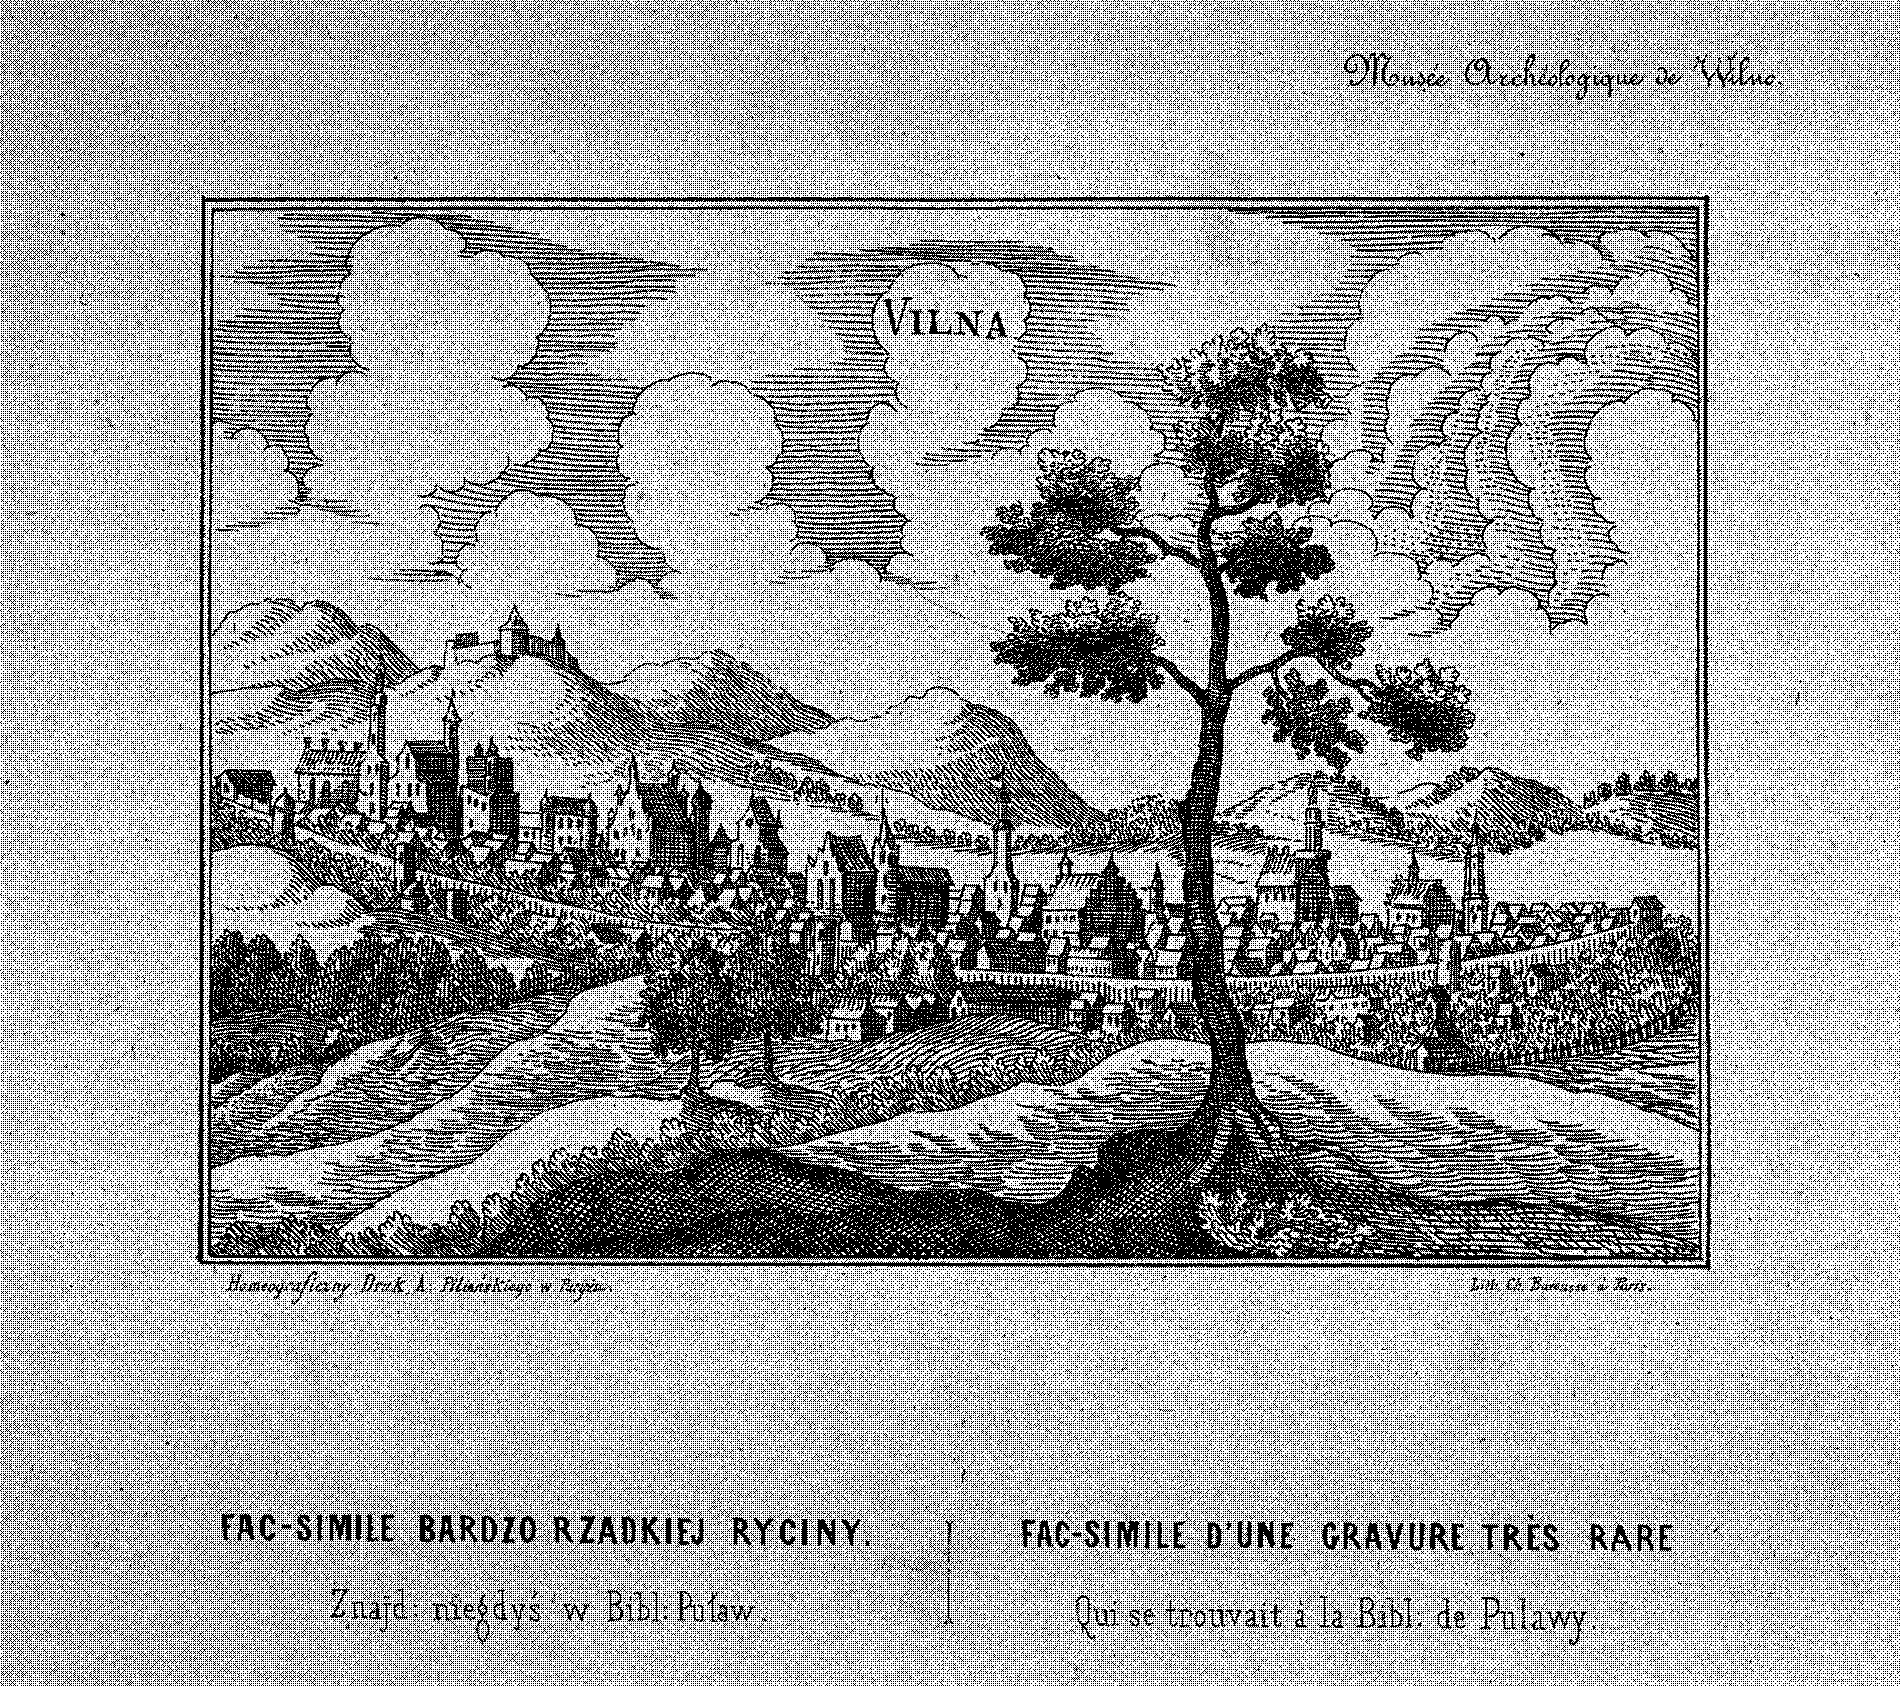
\includegraphics[width=10cm]{./ilustra-11.png} São Paulo\quad2021}
% \end{center}

\begin{figure}[!h]
    \centering
    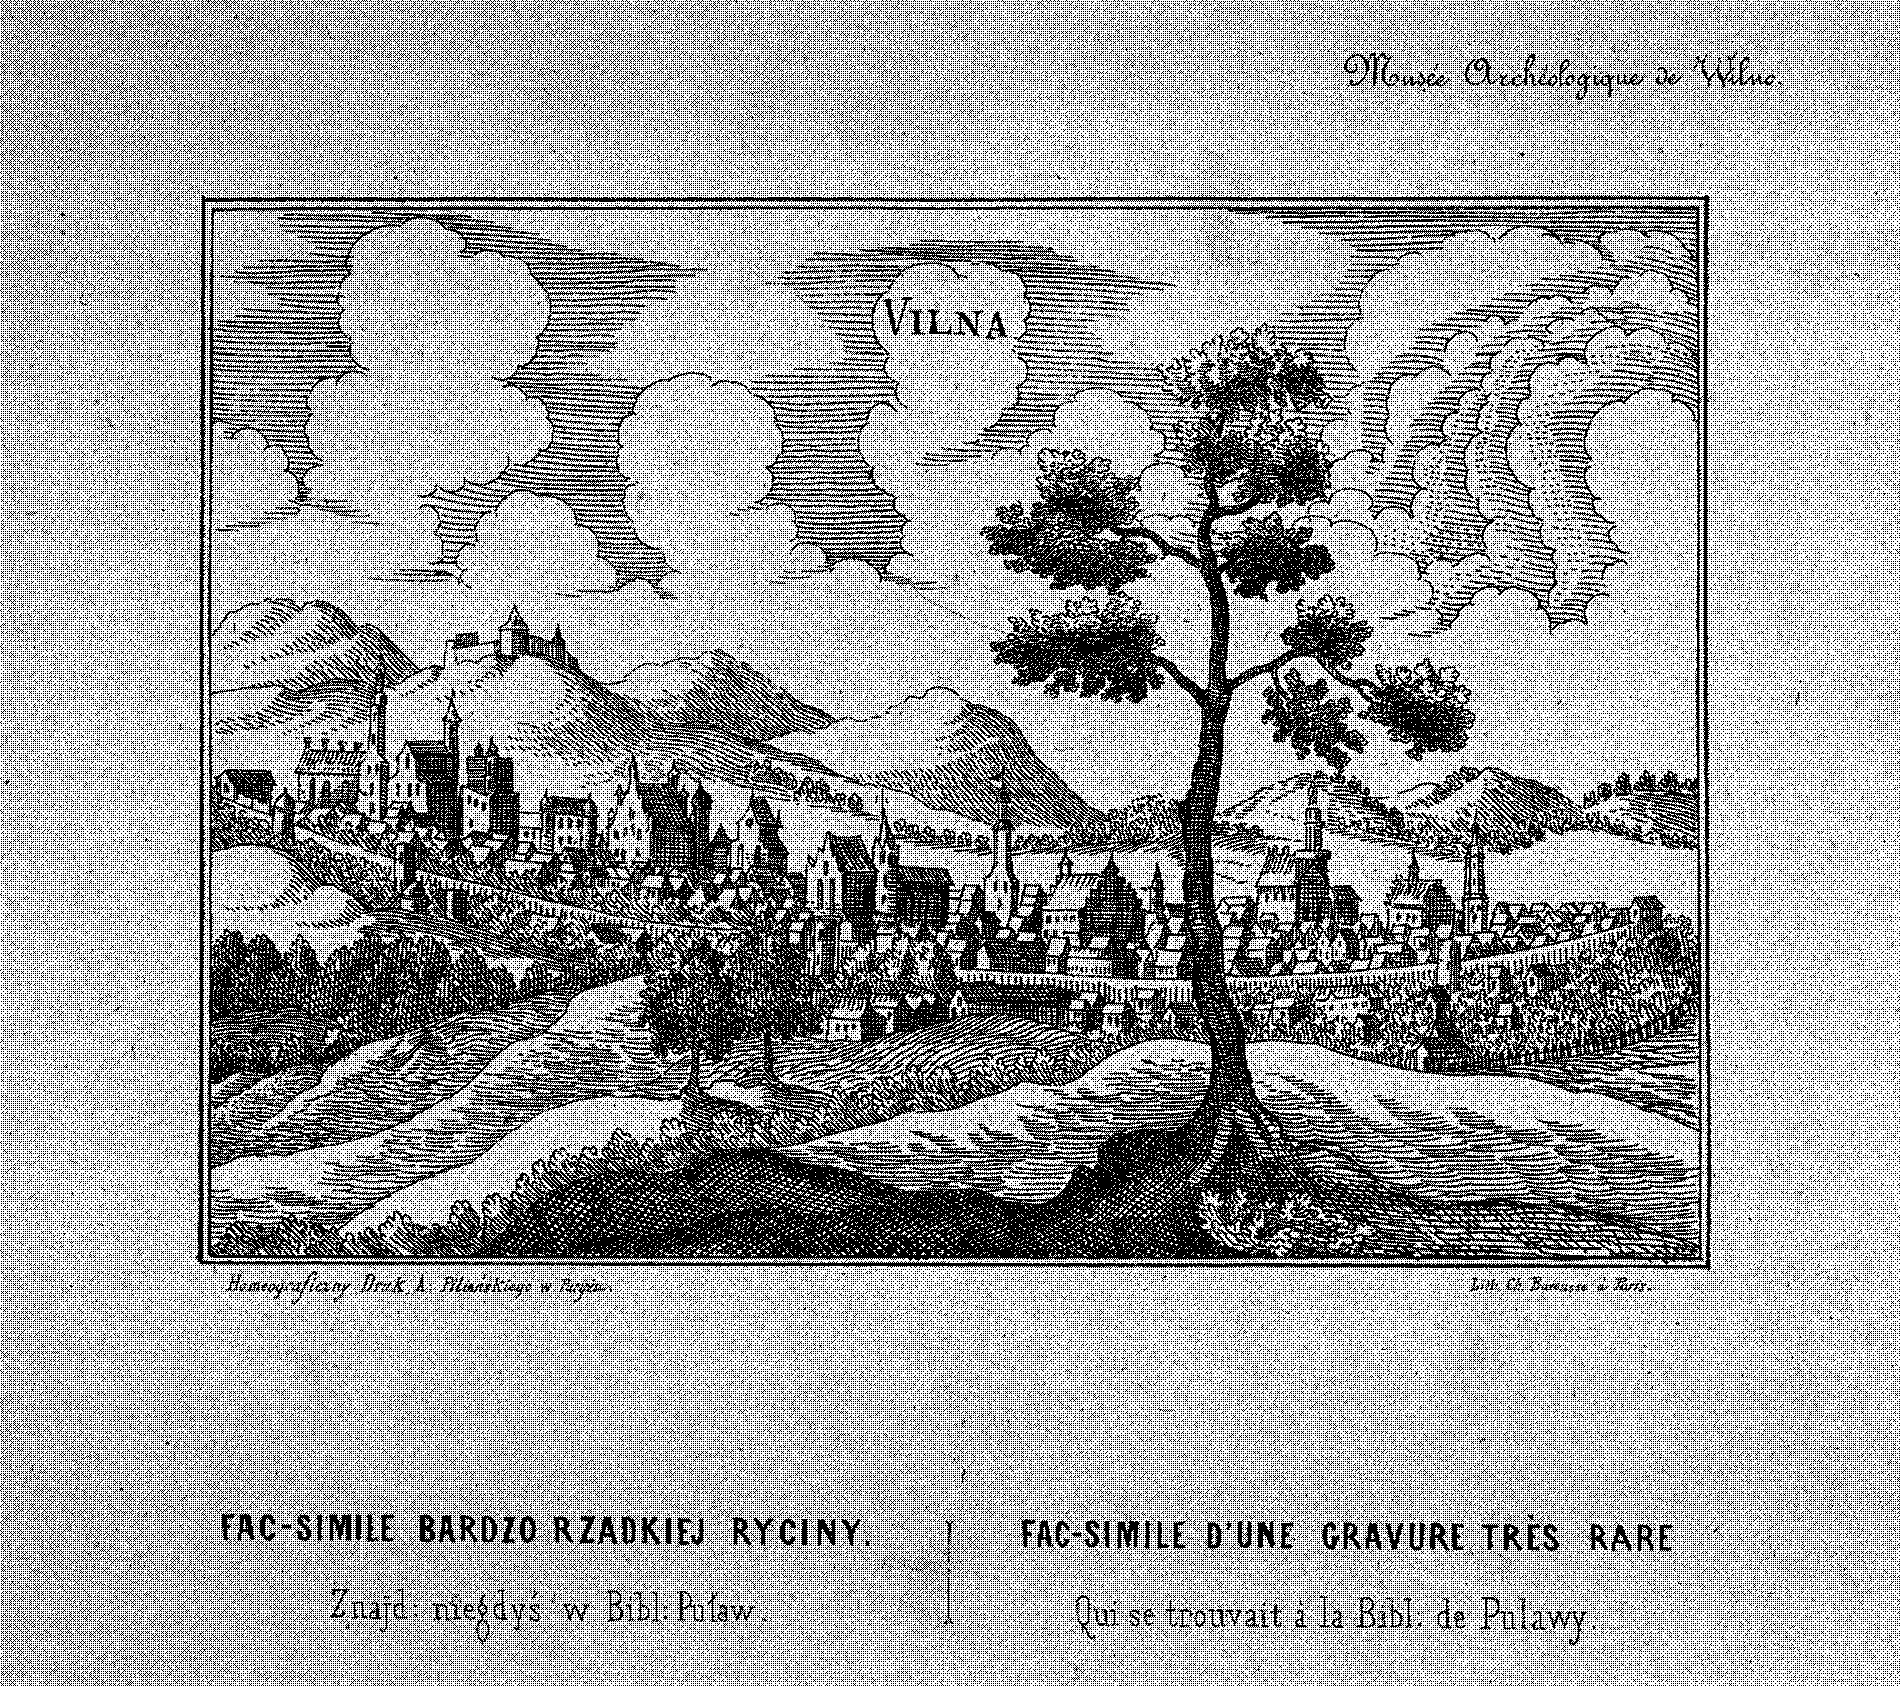
\includegraphics[width=\textwidth]{ilustra-11.png}
    \caption{Vilna e suas árvores de carvalho. Reimpressão do século \textsc {xix} de imagem do século \textsc {xvii}, de artista desconhecido.}
\end{figure}

Apesar do fato de ``pertencerem'' à Europa, os restos estão sob custódia
conjunta franco"-lituana. Descartou"-se a possibilidade de levar os restos
multinacionais para a França e, tendo em vista que a lei francesa não
permite a cremação de soldados franceses, foi decidido sepultá"-los de
novo na Lituânia. Após análise científica minuciosa, o sepultamento
cerimonial dos restos ocorreu em 1 de junho de 2003. Eles agora
descansam no mais variado, do ponto de vista ideológico e nacional,
cemitério de \textit{Vilnius}. Oportunamente, esse grande cemitério, conhecido
como Cemitério dos Soldados, abriga os restos de soldados de diversas
guerras e nacionalidades. Mas, ao lado de tropas alemãs, russas,
polonesas e soviéticas, e agora também napoleônicas, há também túmulos
de autoridades do partido comunista lituano, membros da elite cultural e
acadêmica, e vítimas do ataque de 1991 do exército soviético em \textit{Vilnius}.
O governo francês pagou cerca de sessenta mil euros pelo memorial e,
embora a cerimônia fúnebre tenha sido orquestrada pelo município de
Vilnius, ela seguiu em detalhe as instruções oficiais francesas
concernentes a procedimentos de sepultamento para soldados franceses
tombados. Muitas autoridades de estado lituanas, membros do corpo
diplomático de quase todos os países europeus e representantes da
Sociedade Napoleônica da França participaram da cerimônia. Sacerdotes
benzeram o solo e, em sua alocução, Jean Bernard Harth, embaixador
francês na Lituânia, traçou um paralelo entre 1812 e 2003, referindo"-se
ao apoio de noventa por cento dos lituanos num recenseamento, realizado
três semanas antes, pela adesão à \versal{ue}. Os participantes da cerimônia
fúnebre foram cuidadosamente recordados das falácias da guerra e dos
perigos de uma integração forçada da Europa: ``Napoleão estava em busca
de uma Europa unida,'' observou o embaixador, ``mas seu intuito
fracassou ao tentar unir um continente à força. [\ldots{}] Hoje, vemos
este sonho de uma Europa unida se realizando porque é feito de maneira
pacífica.''\footnote{Conforme citado em Ian Traynor, ``Frozen victims of 1812 get final burial'' em \textit{The Guardian}, 2 de junho de 2003, \textit{www.guardian.co.uk,} acessado em 2 de junho de 2003.}

No entanto, esse sombrio ritual comemorativo ricocheteou de volta para a
cidade como um espetáculo que celebrava a guerra como componente
importante da consolidação política europeia. O sepultamento dos restos
se tornou parte integrante da celebração oficial denominada ``Vilnius
1812'', que tinha a intenção de familiarizar os cidadãos da Lituânia com
a história da breve ocupação francesa na cidade. O evento, que durou
três dias, tencionava também celebrar \textit{Vilnius} como pivô geopolítico que
havia alterado a história lituana e europeia. O principal organizador e
patrocinador da celebração foi o Ministério da Defesa lituano, e o auge
da festa urbana foi a reconstituição cênica de uma batalha entre as
forças ``francesas'' e ``russas'' na margem direita do rio Neris (na
mesma área em que se encontra o novo edifício da prefeitura e um centro
moderno de negócios e diversões próximo à Praça da Europa). Desde 1812,
não houve nenhuma batalha entre os dois exércitos em \textit{Vilnius} ou em seus
arredores, de modo que a representação da batalha foi não só um drama de
mentira, mas uma farsa histórica. Ademais, antes do festival, o Ministro
da Defesa lituano bravamente declarou que ``a marcha do exército de
Napoleão pela Lituânia trouxe um vento de liberdade e a possibilidade de
libertação. Além disso, ofereceu à Lituânia a oportunidade de se
aproximar da Europa.''\footnote{Linas Linkevičius, citado a partir da conferência de imprensa ``Vilnius 1812'' no Ministério da Defesa lituano, 22 de maio de 2003.}

Num gesto contrário, alguns mortos locais se recusaram a levar \textit{Vilnius}
para a Europa sem uma mancha de vergonha. Um novo projeto imobiliário
comercial transformou a vizinhança do cemitério judaico erradicado --- um
dos mais antigos cemitérios da Europa, que abrigava a tumba do Gaon de
\textit{Vilne} --- em zona imobiliária de luxo. A necrópole, localizada do outro
lado do rio a partir da Colina do Castelo, foi desativada pelas
autoridades soviéticas décadas atrás, e não há claro indício de que
todas as relíquias tenham sido removidas. Mas mesmo que nenhum corpo
ainda habite o lugar, ele é mesmo assim testemunho da presença judaica
na cidade com sua memória nua e profanada de aniquilação. Por razões
óbvias, diversos grupos judaicos despertaram a conscientização global
quanto ao projeto e, em resposta, o Congresso dos Estados Unidos ameaçou
a Lituânia de censura política. O governo lituano convocou geólogos
(especialistas em fenômenos naturais) a fim de estabelecer a localização
exata do cemitério, visto que as autoridades municipais consideraram
inadequado e enganoso o trabalho dos arqueólogos (cientistas sociais)
lituanos. A história da cidade se tornou questão de processos
geofísicos, como se a memória e perda humanas fizessem parte do universo
natural, topográfico. Esse ``retorno à natureza'' científico ecoa os
primeiros registros culturais da cidade como lugar perdido num fim de
mundo europeu. A verdade, claro, é menos alegórica: no ímpeto de obter
lucros imobiliários, a cidade transformou os judeus em estrangeiros
locais, nômades mortos sem um lugar que pudessem chamar de lar.

A interação geo"-narrativa de \textit{Vilnius} entre ``estrangeiros locais'' e
``nativos estrangeiros'' foi admiravelmente capturada por Johannes
Bobrowski (1917--1965), poeta alemão cuja relação com a terra mitológica
da Sarmácia se formou graças a um sentido profundo de reparação
histórica e pessoal. Em 1961, publicou seu primeiro ciclo de poemas,
intitulado \textit{Sarmatische Zeit} (\textit{Tempo Sarmácio}), dedicado a
seus encontros, ao longo de toda a vida, com a Sarmácia. Em poucas
palavras, o ciclo poético captura as vastas experiências geográficas e
emocionais do poeta como soldado da \textit{Wehrmacht} no Fronte Oriental
e como prisioneiro de guerra na União Soviética. Bobrowski, porém,
segundo ele mesmo, via seus versos como reparação meditativa e mediadora
dos encontros históricos dos alemães com os vizinhos orientais: ``Isso
se tornou um tema, mais ou menos assim: os alemães e o Leste europeu ---
pois cresci perto do rio Memel, onde poloneses, lituanos, russos e
alemães viveram juntos, e em meio a eles todos, os judeus --- uma longa
história de culpa e desgraça, pela qual meu povo deve ser culpado, desde
os primórdios da Ordem dos Cavaleiros Teutônicos. Algo que não poderá
ser desfeito e nem, talvez, redimido, mas digno de esperança e sincero
empenho em poemas em alemão.''\footnote{Johannes Bobrowski conforme citado em Michael Hamburger, ``Introduction'' em Johannes Bobrowski, \textit{Shadow Lands: Selected Poems}, trad. Ruth e Matthew Mead. Nova York: New Directions Books, 1984, p. 16.}

Para Bobrowski, a história e a geografia local europeias se fundem na
Sarmácia, criando um espaço narrativo que destranca um limiar, um
terreno ampliado de imagens, experiências, nomes de lugares, línguas,
memórias, estórias, biografias, rostos, vozes e traços naturais. É um
tempo"-espaço de descobertas e evocações, mas também de perdas e mudanças
irreversíveis. Ele se põe portanto a desenhar o mapa da Sarmácia com um
poema que começa com uma característica toponímica da cidade e termina
com uma profecia:

%{[}figura 76{]}
%
%Vilna conforme um artista desconhecido do século 17.
\begin{verse}
Vilna, você\\
carvalho ---\\
minha bétula,\\
Novgorod ---\\
certa vez no bosque o grito\\
das minhas primaveras se alçou, o passo\\
dos meus dias ressoou sobre o rio.\\[10pt]
Ó, o brilho\\
cintilante, a constelação estiva,\\
doado; junto ao fogo\\
se agacha o contador de estórias,\\
os que escutaram a noite toda, os jovens,\\
foram embora.\\[10pt]
Sozinho ele cantará:\\
Pela estepe\\
viajam lobos, o caçador\\
achou uma pedra amarela,\\
Incendiou"-se ao luar. ---\\[10pt]
O que é sagrado nada,\\
um peixe,\\
pelos vales antigos, os vales\\
ainda arborizados, as palavras\\
do pai ainda ressoam:\\
Bem"-vindos os estrangeiros!\\
Você será um estrangeiro. Em breve.\footnote{Ibid., ``Chamado'', p.\,23.}
\end{verse}

\chapter{Agradecimentos}

Foi a paisagem urbana de Vilna que guiou o meu trabalho. Contudo, assumo
toda a responsabilidade por qualquer imprecisão no mapa que confeccionei
de sua história. Sou grato àqueles que leram e comentaram as diferentes
versões do manuscrito: Derek Gregory, Modris Eksteins, Thomas Salumets,
Gerry Pratt e Robert North. Pelo auxílio oferecido em suas áreas de
especialidade, gostaria de agradecer Elizabeth Novickas, Aida Novickas,
Dalia Šimavičiūtė, Ernesta Bražėnaitė, Austėja Pečiūra, Fayette Hickox,
Cecile Kuznitz, Antanas Sileika, Violeta Kelertas, Antanas Kubilas,
Juozas Statkevičius, Inga Vidugirytė-Pakerienė, Jurgis Pakerys, Judita e
Eugenijus Čuplinskas, Kristina Sabaliauskaitė, Mindaugas Kvietkauskas,
Alma Lapinskienė, Péter Inkei, Irena Veisaitė, Leonidas Donskis, Laima
Vincė, Darius Ross, Dovilė Kėdikaitė, Jadvyga Dragūnas, e Aida,
Kęstutis, Jonas e Mona Ivinskis. O apoio de minha família foi essencial
para me ajudar a concluir o manuscrito, e pude contar também com a
competente contribuição das equipes da Biblioteca da Universidade de
Vilna, do Museu Lituano de Arte, do Museu Nacional da Lituânia, da
Biblioteca da Academia Lituana de Ciências e do Instituto de Literatura
e Folclore Lituanos. A pesquisa para este livro foi parcialmente
financiada por bolsas de doutorado e pós"-doutorado do Conselho Canadense
de Pesquisas em Ciência Social e Humanidades.


\chapter{Obras citadas}

\begin{bibliohedra}
 \tit{abramowicz}, Hirsz. \textit{Profiles of a Lost World, Memoirs of East
  European Jewish Life before World War \versal{ii}}, trad. Eva Zeitlin Dobkin. Detroit: Wayne University
  Press, 1999.

  \tit{albrecht}, Dietmar. \textit{Wege nach Sarmatien -- Zehn Kapitel
  Preussenland: Orte, Texte, Zeichen}. Munique: Martin Meidenbauer,
  2006.

  \tit{applebaum}, Anne. \textit{Between East and West: Across the Borderlands
  of Europe}. Nova York: Pantheon Books, 1994.

  \tit{austin}, Paul Britten. \textit{1812: the March on Moscow}. Londres:
  Greenhill Books, 1993.

  \titidem. \textit{1812: the Great Retreat}. Londres:
  Greenhill Books, 1996.

  \tit{benedictsen}, Age Meyer. \textit{Lithuania, ``The Awakening of a Nation''
  -- a Study of the Past and Present of the Lithuanian People}.
  Copenhagen: Egmont \textsc{h}.\,Petersens, 1924.

  \tit{bieliūnienė}, Aldona. \textit{Lithuania on the Map}. Vilna:
  Lietuvos nacionalinis muziejus, 1999.

  \tit{bobrowski}, Johannes. \textit{Shadow Lands: Selected Poems.} Trad. Ruth e
  Matthew Mead. Nova York: New Directions Books, 1984.

  \tit{bonosky}, Phillipe. \textit{Beyond the Borders of Myth: from Vilnius to
  Hanoi}. Nova York: Praxis Press, 1967.

  \tit{bourgogne}. \textit{Memoir of Sergeant Bourgogne}, Londres: Jonathan Cape,
  1940 {[}1896{]}.

  \tit{brenner}, David. \textit{Marketing Identities: the Invention of Jewish
  Ethnicity in `Ost und West'}. Detroit: Wayne State University Press,
  1998.

  \tit{brodsky}, Joseph. \textit{A Part of Speech}. Nova York: Farrar, Straus,
  Giroux, 1980.

  \tit{bryusov}, Valery. \textit{Sem' tsvetov radugi: stikhi 1912--1915}. Moscou:
  Izdatelstvo K.\,F. Nekrasova, 1916.

  \tit{bułhak}, Jan. \textit{Vilniaus peizažas: fotografo kelionės}. Vilna:
  Vaga, 2006.

  \tit{campbell}, Thomas. ``Poland'' em \textit{English Romantic Writers}. Nova York: Harcourt, Brace, Janovich, 1967.

  \tit{čepėnas}, Petras. \textit{Naujųjų laikų Lietuvos istorija, t. \versal{ii}}.
  Vilna: Mokslo ir enciklopedijų leidykla, 1992.

  \tit{chesterton}, Gilbert Keith. \textit{Autobiography}. Londres: Hutchinson
  and Company, 1936.

  \tit{chicherin}, Aleksandr. \textit{Dnevnik Aleksandra Chicherina.} Ed.\,S.\,G.
  Engel, M.\,I. Perper, L.\,G. Beskrovny. Moscou: Nauka, 1966.

  \tit{christiansen}, Eric. \textit{The Northern Crusades.} Londres: Penguin
  Books, 1997.

  \tit{čiurinskas}, Mintautas. \textit{Ankstyvieji Šv. Kazimiero
  ``gyvenimai''}. Vilna: Aidai, 2004.

  \tit{clark}, Katerina e Holquist, Michael. \textit{Mikhail Bakhtin}.
  Cambridge: Harvard University Press, 1984.

  \tit{cohen}, Israel. \textit{Vilna}. Filadélfia: The Jewish Publication
  Society of America, 1992.

  \tit{coxe}, William. \textit{Travels in Poland, Russia, Sweden and Denmark}.
  Londres: \textsc{j}.\,Nicholas, 1784.

  \tit{daugirdas}, Romas. ``The Iron Dog, to Vilnius'', trad. Antanas
  Danielius em \textit{Vilna: Lithuanian Literature, Culture, History},
  verão de 1997.

  \tit{davidov}, Denis. \textit{In the Service of the Tsar against Napoleon: the
  Memoirs of Denis Davidov, 1806--1814.}, trad. Gregory Troubetzkoy.
  Londres: Greenhill Books, 1999.

  \tit{davies}, Norman. \textit{God's Playground: A History of Poland}, vol. 1.
  Nova York: Columbia University Press, 1982.

  \titidem. \textit{Heart of Europe: the Past in Poland's Present}.
  Oxford: Oxford University Press, 2001.

  \tit{dawidowicz}, Lucy. \textit{From That Place and Time: A Memoir,
  1939--1947}. Nova York: W.\,W. Norton \& Company, 1989.

  \tit{dembkowski}, Harry \textsc{e}. \textit{The Union of Lublin: Polish Federalism in
  the Golden Age}. Boulder: East European Monographs, 1982.

  \tit{döblin}, Alfred. \textit{Destiny's Journey}, trad. Edgar Passler. Nova
  York: Paragon House, 1992.

  \titidem. \textit{Journey to Poland}, trad. Joachim Neugroschel.
  Nova York: Paragon House, 1991.

  \tit{dobryanski}, C.\,F. \textit{K istorii otechestvenoi voiny. Sostoyania
  Vilny v 1812 g. -- Zapiski Sev.-zapadnovo otdeleniia imperatorskovo
  russkovo geografichestkovo o"-va}, livro 3. Vilna: 1912.

  \titidem. \textit{Staraja i Novaja Vilna}. Vilna: Typografia A.\,G.
  Syrkina, 1904.

  \tit{dobujinsky}, Mstislav. \textit{Vospominaniya, vol. 1}. Nova York: Put'
  Zhizni, 1976.

  \tit{dostoevskaya}, Anna. \textit{Dnevnik 1867 goda}.
  Moscou: Nauka, 1993.

  \tit{dostoiévski}, Fiódor. \textit{The Brothers Karamazov}. Trad. David
  Magarshack. Londres: Penguin Books, 1982.

  \tit{eksteins}, Modris. \textit{Rites of Spring: The Great War and the Birth
  of the Modern Age}. Nova York: Anchor Books, 1990.

  \tit{fezensac}, \textsc{m}.\,\textit{The Russian Campaign, 1812}, trad. Lee Kennett.
  Athens: University of Georgia Press, 1970.

  \tit{ffinch}, Michael. \textit{G.\,K. Chesterton}. Londres: Weidenfeld and
  Nicholson, 1986.

  \tit{forster}, Georg. \textit{Georg Forster Werke: Sämtliche Schriften,
  Tagebücher, Briefe}, vol. 12. Berlim: Akademie
  Verlag, 1978.

  \titidem. \textit{Georg Forsters Werke 15}.
  Berlim: Akademie Verlag, 1981.

  \titidem. \textit{Georg Forsters Werke: Sämtliche Schriften,
  Tagebücher, Briefe (Briefe 1784 -- Juni 1787)}, vol. 14. Berlim: Akademie Verlag, 1978.

  \titidem. \textit{A Voyage Round the World}, vol. 1. Honolulu:
  University of Hawai'I Press, 2000.

  \tit{frank}, Joseph. \textit{Dostoevsky: the Seeds of Revolt, 1821--1849}.
  Princeton University Press, 1976.

  \titidem. \textit{Dostoevsky: the Miraculous Years, 1865--1871}.
  Princeton: Princeton University Press, 1995.

  \tit{frankas}, Josefas (Josef Frank). \textit{Atsiminimai apie Vilnių}, trad.
  Genovaitė Dručkutė. Vilna: Mintis, 2001.

  \tit{friedlander}, Judith. \textit{Vilna on the Seine: Jewish Intellectuals in
  France since 1968}. New Haven: Yale University Press, 1990.

  \tit{goldstein}, David. \textit{Dostoevsky and the Jews}. Austin: University
  of Texas Press, 1981.

  \tit{graben}, Heinz. ``Introduction'' em Alfred Döblin, \textit{Journey to
  Poland}, trad. Joachim Neugroschel. Nova York: Paragon House, 1991.

  \tit{grade}, Chaim. \textit{My Mother's Sabbath Days}, trad. Channa Kleinerman
  Goldstein e Inna Hecker Grade. Nova York: Alfred A. Knopf, 1986.

  \tit{graham}, Stephen. \textit{Russia and the World}. Nova York: The Macmillan
  Company, 1915.

  \tit{grandhomme}, Jean"-Noel. ``Vilnius 1915--1918 m. seno kareivio iš Elzaso
  prisiminimai'' em \textit{Metai}, julho de 2000.

  \tit{grass}, Günter. \textit{The Call of the Toad}, trad. Ralph Manheim. Nova
  York: Harcourt Brace \& Company, 1992

  \tit{hale}, John. \textit{The Civilization of Europe in the Renaissance}. Nova
  York: Atheneum, 1994.

  \tit{Handbook for Travellers in Russia, Poland and Finland}. Londres:
  John Murray, 1867.

  \tit{harshav}, Benjamin. ``Preface'' em Herman Kruk, \textit{The Last Days of
  the Jerusalem of Lithuania: Chronicles from the Vilna Ghetto and the
  Camps, 1939--1944}. New
  Haven: Yale University Press, 2002.

  \tit{herberstein}, Sigismund. \textit{Notes upon Russia: being a translation
  of the earliest account of that country, entitled Rerum Moscoviticarum
  commentarii}, trad. R.\,H. Major. Nova York: Burt
  Franklin, 1963.

  \tit{jacobson}, Dan. \textit{Heshel's Kingdom}. Londres: Penguin Books, 1998.

  \tit{jankevičienė}, Algė, ed., \textit{Vilniaus architektūra}. Vilna:
  Mokslas, 1985.

  \tit{joannes}, Boemus. \textit{The manners, lawes and customs of all nations
  with many other things\ldots{}} Londres: 1611.

  \tit{jurginis}, \textsc{j}., Merkys, \textsc{v}. e Tautavičius, \textsc{a}. \textit{Vilniaus miesto
  istorija: nuo seniausių laikų iki Spalio revoliucijos}. Vilna:
  Mintis, 1968.

  \titidem e \textsc{šidlauskas}, Algirdas, ed., \textit{Kraštas ir
  žmonės}. Vilna: Mokslas, 1983.

  \tit{jurkštas}, Jonas. \textit{Vilniaus vietovardžiai}. Vilna: Mokslas,
  1985.

  \tit{kaufmann}, Thomas da Costa. \textit{Court, Cloister and City: The Art and
  Culture of Central Europe, 1450--1800}. Chicago: University of Chicago
  Press, 1995.

  \tit{klimas}, Petras. \textit{Iš mano atsiminimų}. Vilna: Lietuvos
  enciklopedijų redakcija, 1990.

  \tit{kruk}, Hermann. \textit{The Last Days of the Jerusalem of Lithuania:
  Chronicles from the Vilna Ghetto and the Camps 1939--1944}, ed.
  Benjamin Harshav, trad. Barbara Harshav. New Haven: Yale University
  Press, 2002.

  \tit{kudrinskii}, O.\,A. \textit{Vilna v 1812 godu}. Vilna: 1912.

  \tit{kuznitz}, Cecile \textsc{e}. ``On the Jewish Street: Yiddish culture and the
  urban landscape of interwar Vilna'' em \textit{Yiddish Language and
  Culture: Then and Now}. Creighton: Creighton University Press, 1998.

  \tit{labaume}, Eugene. \textit{The Campaign in Russia}. Londres: Samuel Leigh
  in the Strand, 1815.

  \tit{lachmann}, Renate. \textit{Memory and Literature: Intertextuality in
  Russian Modernism}, trad. Roy Sellars e Anthony Wall. Minneapolis:
  University of Minnesota Press, 1997.

  \tit{lavrinec}, Pavel. Ed. \textit{Russkaja literature v Litve \versal{xiv}--\versal{xx} v}.
  Vilna: Lietuvos Rašytojų Sąjungos Leidykla, 1998

  \tit{lieven}, Anatol. \textit{The Baltic Revolution: Estonia, Latvia,
  Lithuania and the Path to Independence}. New Haven: Yale University
  Press, 1993.

  \tit{liulevicius}, Vejas. \textit{War Land on the Eastern Front: Culture,
  National Identity and German Occupation}. Cambridge: Cambridge
  University Press, 2001.

  \tit{ludendorff}, Erich. \textit{My War Memories}, vol. 1--2. Londres:
  Hutchinson \& Co., 1919.

  \tit{mann}, Thomas. \textit{Buddenbrooks: the Decline of a Family}, trad. John
  \textsc{e}. Woods. Nova York: Knopf, 1993.

  \tit{martinaitienė}, Gražina Marija. ``At the crossings of western and
  eastern cultures: the contush sashes'' em \textit{Lietuvos Didžiosios
  Kunigaikštystės barokas: formos, įtakos kryptys.} Acta Academiae
  Artium Vilnensis 21, 2001.

  \tit{masionienė}, Birutė. ``F. Dostojevskio kilmės klausimu'' em
  \textit{Literatūrinių ryšių pėdsakais}. Vilna: Vaga, 1982.

  \titidem. \textit{Levas Tolstojus ir Lietuva}. Vilna: Vaga,
  1978.

  \tit{matušakaitė}, Marija. \textit{Apranga \versal{xvi}--\versal{xviii} a. Lietuvoje}. Vilna:
  Aidai, 2003.

  \tit{mcbride}, Robert Medill. \textit{Towns and People of Modern Poland}. Nova
  York: McBride and Company, 1938.

  \tit{metelsky}, \textsc{g}. \textit{Lithuania: Land of the Niemen}. Moscou: Foreign
  Languages Publishing House, 1959.

  \tit{miłosz}, Czesław. \textit{Beginning with My Streets}, trad. Madeline G.
  Levine. Nova York: Farrar Straus Giroux, 1991.

  \tit{minczeles}, Henri. ``A journey into the heart of Yiddishland'' em
  \textit{Yiddishland}, ed. Gerrard Silvain e Henri Minczeles. Corte
  Madera, California: Gingko Press, 1999.

  \tit{monty}, Paul. \textit{Wanderstunden in Wilna}. Vilna: Verlag der Wilnaer
  Zeitung, 1918.

  \tit{ostrovsky}, Aleksandr. \textit{Polnoje sobranije t. 10}. Moscou: Isskustvo, 1978.

  \tit{pares}, Bernard. \textit{Day by Day with Russian Army, 1914--1915}.
  Londres: Constable \& Company, 1915.

  \tit{pašuta} \textsc{v}. e \textsc{i}.\,Štal, ed., \textit{Gedimino laiškai.} Vilna: Mintis,
  1966.

  \tit{persky}, Stan. \textit{Then We Take Berlin: Stories from the Other Side
  of Europe}. Toronto: Alfred Knopf, 1995.

  \tit{``polskij Vopros''} em \textit{Severnaya Pchela}, 5 de maio de 1863.

  \tit{ragauskas}, Aivas. \textit{Vilniaus miesto valdantysis elitas: \versal{xvii} a.
  antrojoje pusėje}. Vilna: Diemedžio leidykla, 2002.

  \tit{``Rasti palaikai -- daugelio tautų paveldas''} em \textit{Lietuvos rytas},
  30 de março de 2002.

  \tit{riley"-smith}, Jonathan. \textit{The Crusades: A History}. New Haven: Yale
  University Press, 2005.

  \tit{römeris}, Mykolas. \textit{Dienoraštis}, trad. Vaiva Grigaitienė.
  Vilna: Versus Aureus, 2007.

  \tit{roth}, Joseph. \textit{The Wandering Jews}, trad. Michael Hofmann. Nova
  York: W.\,W. Norton, 2001.

  \tit{roy}, James Charles. \textit{The Vanished Kingdom: Travels through the
  History of Prussia}. Boulder: Westview Press, 1999.

  \tit{rudashevski}, Yitskhok em \textit{Children in the Holocaust and World
  War \versal{ii}: Their Secret Diaries}. Nova York: Pocket
  Books, 1995.

  \tit{saine}, Thomas \textsc{f}. \textit{Georg Forster}. Nova York: Twayne Publishers,
  1972.

  \tit{saisselin}, Remy \textsc{g}. \textit{The Enlightenment against Baroque: Economics
  and Aesthetics of the Eighteenth Century}. Berkeley: University of
  California Press, 1992.

  \tit{sas}, A. ``Poezdka v Vilno'' em \textit{Severnaya Pchela}, 5 de maio de
  1863.

  \tit{schauss}, Hayyim. \textit{The Jewish Festivals: History and Observance}.
  Nova York: Schocken Books, 1975.

  \tit{schedel}, Hartmann. \textit{Sarmatia}, e o capítulo sarmácio de
  \textit{Liber chronicarum} impresso em Nurembergue por Anton Koberger em
  1493, traduzido e editado por \textsc{b}.\,Deresiewicz, Londres: Oficyna
  Stanisław Gliwa, 1973.

  \tit{segur}, Phillipe"-Paul. \textit{Napoleon's Russian Campaign}. Trad. J.
  David Townsend. Londres: Michael Joseph, 1959.

  \tit{stendhal}. \textit{To the Happy Few: Selected Letters of Stendhal}. Nova
  York: Grove Press, 1952.

  \tit{stone}, Daniel. \textit{The Polish"-Lithuanian State, 1386--1795}. Seattle:
  University of Washington Press, 2001.

  \tit{strong}, Anne Louise. \textit{Lithuania's New Way}. Londres: Lawrence \&
  Wishart, 1940.

  \tit{The Story of Wilno}. The Polish Research Centre. Londres:
  Lawrence \& Wishart, 1940.

  \tit{sukiennicki}, Wiktor. \textit{East Central Europe during World War \versal{i}:
  from Foreign Domination to National Independence, vol. 2}. Nova York:
  Columbia University Press, 1984.

  \tit{tarm}, \textsc{m}. ``The Napoleon graves'' em \textit{City Paper: The Baltic
  States}, novembro de 2002.

  \tit{tereškinas}, Artūras. \textit{Imperfect Communities: Identity, Discourse
  and Nation in the Seventeenth"-Century Grand Duchy of Lithuania}.
  Vilna: Lietuvių literatūros ir tautosakos institutas, 2005.

  \tit{tolstói}, Liev. \textit{War and Peace}. Trad. Constance Garnett. Nova York:
  The Modern Library, 2002.

  \tit{toporov}, Vladimir. Baltų mitologijos ir ritualo tyrimai. Vilna:
  Aidai, 2000.

  \tit{traynor}, Ian. ``Frozen victims of 1812 get final burial'' em \textit{The
  Guardian}, 2 de junho de 2003, \textit{www.guardian.co.uk,} acessado em
  2 de junho de 2003.

  \tit{ulčinaitė}, Eugenija, ed., \textit{Gratulatio Vilne}. Vilna: Lietuvių
  literatūros ir tautosakos institutas, 2001.

  \tit{uxkull}, Boris. \textit{Arms and the Woman: the Intimate Journal of a
  Baltic Nobleman in the Napoleonic Wars}, trad. Joel Carmichael. New
  York: The Macmillan Company, 1966.

  \tit{vaičiūnaitė}, Judita. ``Museum Street'', trad. Jonas Zdanys em
  \textit{Contemporary East European Poetry: An Anthology}. Oxford: Oxford University Press, 1993.

  \tit{vaitiekus}, Severinas. \textit{Tuskulėnai: egzekucijų aukos ir budeliai}.
  Vilna: Lietuvos gyventojų genocido ir rezistencijos tyrimo centras,
  2002.


\tit{vanagas}, Aleksandras. ``Miesto vardas Vilnius'' em \textit{Gimtasis
žodis}, n. 11 (59), novembro, 1993.

\tit{venclova}, Tomas. ``Dialogue about Wilno with Thomas Venclova'' em
Czesław Miłosz, \textit{Beginning with My Streets}, trad. Madeline G.
Levine. Nova York: Farrar Straus Giroux, 1991.

\titidem. \textit{Vilnius: City Guide}. Vilna: \textsc{r}.\,Paknio
leidykla, 2001.

\tit{verdery}, Katherine. \textit{The Political Lives of Dead Bodies: Reburial
and Postsocialist change}. Nova York: Columbia University Press, 1999.

\tit{villari}, Rosario. ``Introduction'' em \textit{Baroque Personae}, ed.
Rosario Villari. Chicago: University of Chicago Press, 1995.

\tit{``Vilnių garsins ir Napoleono palaikai''} em \textit{Lietuvos rytas}, seção
Sostinė, 13 de setembro de 2002.

\tit{vinogradov}, A.\,A. \textit{Putevoditel pe gorodu Vilna i evo okrestnosiam}.
Vilna: Tipografia Shtaba Vilenskavo Voenava Okruga, 1908.

\tit{vossler}, \textsc{h.\,a}. \textit{With Napoleon in Russia in 1812: the Diary of \textsc{lt.\,h.\,a.}\,Vossler, a Soldier of the Grand Army 1812--1813}, trad. Walter
Wallich. Londres: Constable, 1998.

\tit{washburn}, Stanley. \textit{On the Russian Front in the World War \versal{i}:
Memoirs of an American War Correspondent}. Nova York: Robert Speller and
Sons, 1982.

\tit{weber}, Paul, \textit{Wilna: eine vergessene Kunstsstätte}. Vilna: Verlag
der Zeitung der 10. Armee, 1917.

\tit{wilson}, Robert, \textit{General Wilson's Journal, 1812--1814}. Londres: William Kimber, 1964.

\tit{wines}, Michael, ``Baltic soil yields evidence of a bitter end to
Napoleon's Army'' em \textit{New York Times}, 4 de setembro de 2002.

\tit{wolff}, Larry, \textit{Inventing Eastern Europe: The Map of Civilization on
the Mind of the Enlightenment}. Stanford: Stanford University Press,
1994.

\tit{zamoyski}, Adam, \textit{Moscow 1812: Napoleon's Fatal March}. Nova York:
Harper Collins, 2004. \EP[1]

\tit{zwi}, Rose. \textit{Last Walk in Naryshkin Park}. Melbourne:
Spinifex, 1997.
\end{bibliohedra}


%\chapter{Índice remissivo}

%\textbf{Segunda orelha}
%
%Napoleão, Dostoiévski, Stendhal, Tolstói, Döblin, Forster, Bakhtin e
%Brodsky: essas vozes --- entre muitas outras igualmente sedutoras, porém
%menos conhecidas --- revelam a essência da Europa em suas narrativas do
%encontro com a cidade limiar de Vilna. Laimonas Briedis teceu as cartas,
%diários, observações e reflexões de estrangeiros a respeito dessa cidade
%que funciona como portão de entrada para o coração da Europa numa
%estória intimista e atraente. O autor divide com o leitor uma profunda
%compreensão das identidades lituana, polonesa, russa e alemã do lugar,
%assim como sua situação central na cultura judaica europeia. Ricamente
%ilustrado e resultado de pesquisa cuidadosa, este livro é um verdadeiro
%salão de espelhos, que fornece uma visão brilhante de Vilna e uma
%excepcional janela para a Europa.
%
%Laimonas Briedis é natural de Vilna. Doutorou"-se em geografia humana na
%Universidade de British Columbia e concluiu sua pesquisa de
%pós"-doutorado no Departamento de História da Universidade de Toronto.
%Mora em Vilna e em Vancouver, Canadá.
%
%\textbf{Contracapa}
%
%``Livro maravilhoso --- a melhor coisa que já foi publicada sobre Vilna nos
%últimos anos.'' Anatol Lieven, autor de \textit{The Baltic Revolution:
%Estonia, Latvia and Lithuania and the Path to Independence}
%
%``Para uma visita completa a Vilna, tanto visitantes como seus próprios
%habitantes deveriam ter um exemplar deste livro e sair para descobrir a
%história rica, interessante e multicultural da cidade.'' \textit{The
%Baltic Times}
%
%``Contribuição original para a nossa compreensão de uma cidade tão
%complexa\ldots{} fornece esplêndida coleção de provas do passado
%histórico bem como comentários estimulantes sobre acontecimentos mais
%recentes.'' Alan Palmer, autor de \textit{Northern Shores: a History of
%the Baltic Sea and its People}
%
%``Bela fórmula\ldots{} combinando a história da Europa com a geografia
%de Vilna.'' \textit{Radio France Internationale}
%
%``\ldots{} leitura deliciosa\ldots{} os \textit{connaisseurs} da boa
%literatura\ldots{} talvez não consigam parar antes de chegar à última
%página deste fascinante relato histórico.'' Victor H. Winston,
%\textit{European Geography and Economics}
%
%``Finalmente, um livro que não tenta impor uma imagem politicamente
%correta, ultranacionalista e retrospectiva de ``Vilnius'' e seus longos
%séculos como Vilna,  e Wilno\ldots{} deliciosamente escrito, com a
%precisão de um acadêmico e o coração de um contador de estórias.'' Dovid
%Katz, autor de \textit{Words on Fire: the Unfinished Story of Yiddish}
%
%``\ldots{} no livro sutil e evocativo de Briedis\ldots{} Civilizações
%desaparecidas e impérios perdidos deixam uma cidade assombrada pelo
%horror e impregnada de beleza.'' \textit{The Economist}
%
%``Um presente perfeito de Vilna.'' Simon Seabag Montefiore, autor de
%\textit{Jerusalem, the Biography} e \textit{Young Stalin}
}
%\part[{{\def\break{}\titulo}}]{\titulo}
} % fim do AtBeginDocument

% Finais -------------------------------------------------------
\AtEndDocument{%
  %\publicidade

\pagebreak\ifodd\thepage\paginabranca\fi

\ifdef{\imagemficha}{\IfFileExists{\imagemficha}{\includegraphics[width=.7\textwidth]{\imagemficha}\par}}{}

\mbox{}\vfill\small\thispagestyle{empty}
\begin{center}
\begin{minipage}{.8\textwidth}
\centering\tiny\noindent{}Adverte-se aos curiosos que se imprimiu este livro \ifdef{\grafica}{na gráfica \grafica}{em nossas oficinas}, 
em \today \ifdef{\papelmiolo}{em papel \papelmiolo}, em tipologia Formular e \tipopadrao{}, com diversos sofwares livres, 
entre eles, Lua\LaTeX, git \& ruby. \ifdef{\RevisionInfo{}}{\par(v.\,\RevisionInfo)}{}\par \begin{center}\normalsize\adforn{64}\end{center}
\end{minipage}
\end{center}
}

